\documentclass[a4paper]{book}
\usepackage{a4wide}
\usepackage{makeidx}
\usepackage{fancyhdr}
\usepackage{graphicx}
\usepackage{multicol}
\usepackage{float}
\usepackage{textcomp}
\usepackage{alltt}
\usepackage{times}
\usepackage{ifpdf}
\ifpdf
\usepackage[pdftex,
            pagebackref=true,
            colorlinks=true,
            linkcolor=blue,
            unicode
           ]{hyperref}
\else
\usepackage[ps2pdf,
            pagebackref=true,
            colorlinks=true,
            linkcolor=blue,
            unicode
           ]{hyperref}
\usepackage{pspicture}
\fi
\usepackage[utf8]{inputenc}
\usepackage{doxygen}
\makeindex
\setcounter{tocdepth}{3}
\renewcommand{\footrulewidth}{0.4pt}
\begin{document}
\begin{titlepage}
\vspace*{7cm}
\begin{center}
{\Large Hydrax \\[1ex]\large 0.5.1 }\\
\vspace*{1cm}
{\large Generated by Doxygen 1.5.8}\\
\vspace*{0.5cm}
{\small Tue Sep 1 14:19:26 2009}\\
\end{center}
\end{titlepage}
\clearemptydoublepage
\pagenumbering{roman}
\tableofcontents
\clearemptydoublepage
\pagenumbering{arabic}
\chapter{Todo List}
\label{todo}
\hypertarget{todo}{}
\label{todo__todo000001}
\hypertarget{todo__todo000001}{}
 \begin{description}
\item[Member \hyperlink{class_hydrax_1_1_hydrax_c584e30a6cbfb5d8884afb182c29d36a}{Hydrax::Hydrax::update}(const Ogre::Real \&timeSinceLastFrame) ]Add listener interface \end{description}

\chapter{Namespace Index}
\section{Namespace List}
Here is a list of all namespaces with brief descriptions:\begin{CompactList}
\item\contentsline{section}{\hyperlink{namespace_hydrax}{Hydrax} }{\pageref{namespace_hydrax}}{}
\item\contentsline{section}{\hyperlink{namespace_hydrax_1_1_module}{Hydrax::Module} }{\pageref{namespace_hydrax_1_1_module}}{}
\item\contentsline{section}{\hyperlink{namespace_hydrax_1_1_noise}{Hydrax::Noise} }{\pageref{namespace_hydrax_1_1_noise}}{}
\end{CompactList}

\chapter{Class Index}
\section{Class Hierarchy}
This inheritance list is sorted roughly, but not completely, alphabetically:\begin{CompactList}
\item \contentsline{section}{Hydrax::CfgFileManager}{\pageref{class_hydrax_1_1_cfg_file_manager}}{}
\item \contentsline{section}{Hydrax::Decal}{\pageref{class_hydrax_1_1_decal}}{}
\item \contentsline{section}{Hydrax::DecalsManager}{\pageref{class_hydrax_1_1_decals_manager}}{}
\item \contentsline{section}{Hydrax::Noise::FFT::FFT::Options}{\pageref{struct_hydrax_1_1_noise_1_1_f_f_t_1_1_options}}{}
\item \contentsline{section}{Hydrax::GodRaysManager}{\pageref{class_hydrax_1_1_god_rays_manager}}{}
\item \contentsline{section}{Hydrax::GPUNormalMapManager}{\pageref{class_hydrax_1_1_g_p_u_normal_map_manager}}{}
\item \contentsline{section}{Hydrax::Hydrax}{\pageref{class_hydrax_1_1_hydrax}}{}
\item \contentsline{section}{Hydrax::Image}{\pageref{class_hydrax_1_1_image}}{}
\item \contentsline{section}{Hydrax::Image::Image::Pixel}{\pageref{struct_hydrax_1_1_image_1_1_pixel}}{}
\item \contentsline{section}{Hydrax::MaterialManager}{\pageref{class_hydrax_1_1_material_manager}}{}
\item \contentsline{section}{Hydrax::MaterialManager::MaterialManager::Options}{\pageref{struct_hydrax_1_1_material_manager_1_1_options}}{}
\item \contentsline{section}{Hydrax::MaterialManager::MaterialManager::UnderwaterCompositorListener}{\pageref{class_hydrax_1_1_material_manager_1_1_underwater_compositor_listener}}{}
\item \contentsline{section}{Hydrax::Math}{\pageref{class_hydrax_1_1_math}}{}
\item \contentsline{section}{Hydrax::Mesh}{\pageref{class_hydrax_1_1_mesh}}{}
\item \contentsline{section}{Hydrax::Mesh::Mesh::Options}{\pageref{struct_hydrax_1_1_mesh_1_1_options}}{}
\item \contentsline{section}{Hydrax::Mesh::Mesh::POS\_\-NORM\_\-UV\_\-VERTEX}{\pageref{struct_hydrax_1_1_mesh_1_1_p_o_s___n_o_r_m___u_v___v_e_r_t_e_x}}{}
\item \contentsline{section}{Hydrax::Mesh::Mesh::POS\_\-NORM\_\-VERTEX}{\pageref{struct_hydrax_1_1_mesh_1_1_p_o_s___n_o_r_m___v_e_r_t_e_x}}{}
\item \contentsline{section}{Hydrax::Mesh::Mesh::POS\_\-UV\_\-VERTEX}{\pageref{struct_hydrax_1_1_mesh_1_1_p_o_s___u_v___v_e_r_t_e_x}}{}
\item \contentsline{section}{Hydrax::Mesh::Mesh::POS\_\-VERTEX}{\pageref{struct_hydrax_1_1_mesh_1_1_p_o_s___v_e_r_t_e_x}}{}
\item \contentsline{section}{Hydrax::Module::Module}{\pageref{class_hydrax_1_1_module_1_1_module}}{}
\begin{CompactList}
\item \contentsline{section}{Hydrax::Module::ProjectedGrid}{\pageref{class_hydrax_1_1_module_1_1_projected_grid}}{}
\item \contentsline{section}{Hydrax::Module::RadialGrid}{\pageref{class_hydrax_1_1_module_1_1_radial_grid}}{}
\item \contentsline{section}{Hydrax::Module::SimpleGrid}{\pageref{class_hydrax_1_1_module_1_1_simple_grid}}{}
\end{CompactList}
\item \contentsline{section}{Hydrax::Noise::Noise}{\pageref{class_hydrax_1_1_noise_1_1_noise}}{}
\begin{CompactList}
\item \contentsline{section}{Hydrax::Noise::FFT}{\pageref{class_hydrax_1_1_noise_1_1_f_f_t}}{}
\item \contentsline{section}{Hydrax::Noise::Perlin}{\pageref{class_hydrax_1_1_noise_1_1_perlin}}{}
\end{CompactList}
\item \contentsline{section}{Hydrax::Noise::Perlin::Perlin::Options}{\pageref{struct_hydrax_1_1_noise_1_1_perlin_1_1_options}}{}
\item \contentsline{section}{Hydrax::Module::ProjectedGrid::ProjectedGrid::Options}{\pageref{struct_hydrax_1_1_module_1_1_projected_grid_1_1_options}}{}
\item \contentsline{section}{Hydrax::Module::RadialGrid::RadialGrid::Options}{\pageref{struct_hydrax_1_1_module_1_1_radial_grid_1_1_options}}{}
\item \contentsline{section}{Hydrax::RttManager}{\pageref{class_hydrax_1_1_rtt_manager}}{}
\item \contentsline{section}{Hydrax::RttManager::RttManager::CReflectionListener::RttManager::CReflectionListener::CReflectionQueueListener}{\pageref{class_hydrax_1_1_rtt_manager_1_1_c_reflection_listener_1_1_c_reflection_queue_listener}}{}
\item \contentsline{section}{Hydrax::RttManager::RttManager::RttListener}{\pageref{class_hydrax_1_1_rtt_manager_1_1_rtt_listener}}{}
\item \contentsline{section}{Hydrax::RttManager::RttManager::RttOptions}{\pageref{struct_hydrax_1_1_rtt_manager_1_1_rtt_options}}{}
\item \contentsline{section}{Hydrax::Module::SimpleGrid::SimpleGrid::Options}{\pageref{struct_hydrax_1_1_module_1_1_simple_grid_1_1_options}}{}
\item \contentsline{section}{Hydrax::Size}{\pageref{struct_hydrax_1_1_size}}{}
\item \contentsline{section}{Hydrax::TextureManager}{\pageref{class_hydrax_1_1_texture_manager}}{}
\end{CompactList}

\chapter{Class Index}
\section{Class List}
Here are the classes, structs, unions and interfaces with brief descriptions:\begin{CompactList}
\item\contentsline{section}{\hyperlink{class_hydrax_1_1_cfg_file_manager}{Hydrax::CfgFileManager} }{\pageref{class_hydrax_1_1_cfg_file_manager}}{}
\item\contentsline{section}{\hyperlink{class_hydrax_1_1_decal}{Hydrax::Decal} }{\pageref{class_hydrax_1_1_decal}}{}
\item\contentsline{section}{\hyperlink{class_hydrax_1_1_decals_manager}{Hydrax::DecalsManager} }{\pageref{class_hydrax_1_1_decals_manager}}{}
\item\contentsline{section}{\hyperlink{class_hydrax_1_1_noise_1_1_f_f_t}{Hydrax::Noise::FFT} }{\pageref{class_hydrax_1_1_noise_1_1_f_f_t}}{}
\item\contentsline{section}{\hyperlink{struct_hydrax_1_1_noise_1_1_f_f_t_1_1_options}{Hydrax::Noise::FFT::FFT::Options} }{\pageref{struct_hydrax_1_1_noise_1_1_f_f_t_1_1_options}}{}
\item\contentsline{section}{\hyperlink{class_hydrax_1_1_god_rays_manager}{Hydrax::GodRaysManager} }{\pageref{class_hydrax_1_1_god_rays_manager}}{}
\item\contentsline{section}{\hyperlink{class_hydrax_1_1_g_p_u_normal_map_manager}{Hydrax::GPUNormalMapManager} }{\pageref{class_hydrax_1_1_g_p_u_normal_map_manager}}{}
\item\contentsline{section}{\hyperlink{class_hydrax_1_1_hydrax}{Hydrax::Hydrax} }{\pageref{class_hydrax_1_1_hydrax}}{}
\item\contentsline{section}{\hyperlink{class_hydrax_1_1_image}{Hydrax::Image} }{\pageref{class_hydrax_1_1_image}}{}
\item\contentsline{section}{\hyperlink{struct_hydrax_1_1_image_1_1_pixel}{Hydrax::Image::Image::Pixel} }{\pageref{struct_hydrax_1_1_image_1_1_pixel}}{}
\item\contentsline{section}{\hyperlink{class_hydrax_1_1_material_manager}{Hydrax::MaterialManager} }{\pageref{class_hydrax_1_1_material_manager}}{}
\item\contentsline{section}{\hyperlink{struct_hydrax_1_1_material_manager_1_1_options}{Hydrax::MaterialManager::MaterialManager::Options} }{\pageref{struct_hydrax_1_1_material_manager_1_1_options}}{}
\item\contentsline{section}{\hyperlink{class_hydrax_1_1_material_manager_1_1_underwater_compositor_listener}{Hydrax::MaterialManager::MaterialManager::UnderwaterCompositorListener} }{\pageref{class_hydrax_1_1_material_manager_1_1_underwater_compositor_listener}}{}
\item\contentsline{section}{\hyperlink{class_hydrax_1_1_math}{Hydrax::Math} }{\pageref{class_hydrax_1_1_math}}{}
\item\contentsline{section}{\hyperlink{class_hydrax_1_1_mesh}{Hydrax::Mesh} }{\pageref{class_hydrax_1_1_mesh}}{}
\item\contentsline{section}{\hyperlink{struct_hydrax_1_1_mesh_1_1_options}{Hydrax::Mesh::Mesh::Options} }{\pageref{struct_hydrax_1_1_mesh_1_1_options}}{}
\item\contentsline{section}{\hyperlink{struct_hydrax_1_1_mesh_1_1_p_o_s___n_o_r_m___u_v___v_e_r_t_e_x}{Hydrax::Mesh::Mesh::POS\_\-NORM\_\-UV\_\-VERTEX} }{\pageref{struct_hydrax_1_1_mesh_1_1_p_o_s___n_o_r_m___u_v___v_e_r_t_e_x}}{}
\item\contentsline{section}{\hyperlink{struct_hydrax_1_1_mesh_1_1_p_o_s___n_o_r_m___v_e_r_t_e_x}{Hydrax::Mesh::Mesh::POS\_\-NORM\_\-VERTEX} }{\pageref{struct_hydrax_1_1_mesh_1_1_p_o_s___n_o_r_m___v_e_r_t_e_x}}{}
\item\contentsline{section}{\hyperlink{struct_hydrax_1_1_mesh_1_1_p_o_s___u_v___v_e_r_t_e_x}{Hydrax::Mesh::Mesh::POS\_\-UV\_\-VERTEX} }{\pageref{struct_hydrax_1_1_mesh_1_1_p_o_s___u_v___v_e_r_t_e_x}}{}
\item\contentsline{section}{\hyperlink{struct_hydrax_1_1_mesh_1_1_p_o_s___v_e_r_t_e_x}{Hydrax::Mesh::Mesh::POS\_\-VERTEX} }{\pageref{struct_hydrax_1_1_mesh_1_1_p_o_s___v_e_r_t_e_x}}{}
\item\contentsline{section}{\hyperlink{class_hydrax_1_1_module_1_1_module}{Hydrax::Module::Module} }{\pageref{class_hydrax_1_1_module_1_1_module}}{}
\item\contentsline{section}{\hyperlink{class_hydrax_1_1_noise_1_1_noise}{Hydrax::Noise::Noise} }{\pageref{class_hydrax_1_1_noise_1_1_noise}}{}
\item\contentsline{section}{\hyperlink{class_hydrax_1_1_noise_1_1_perlin}{Hydrax::Noise::Perlin} }{\pageref{class_hydrax_1_1_noise_1_1_perlin}}{}
\item\contentsline{section}{\hyperlink{struct_hydrax_1_1_noise_1_1_perlin_1_1_options}{Hydrax::Noise::Perlin::Perlin::Options} }{\pageref{struct_hydrax_1_1_noise_1_1_perlin_1_1_options}}{}
\item\contentsline{section}{\hyperlink{class_hydrax_1_1_module_1_1_projected_grid}{Hydrax::Module::ProjectedGrid} }{\pageref{class_hydrax_1_1_module_1_1_projected_grid}}{}
\item\contentsline{section}{\hyperlink{struct_hydrax_1_1_module_1_1_projected_grid_1_1_options}{Hydrax::Module::ProjectedGrid::ProjectedGrid::Options} }{\pageref{struct_hydrax_1_1_module_1_1_projected_grid_1_1_options}}{}
\item\contentsline{section}{\hyperlink{class_hydrax_1_1_module_1_1_radial_grid}{Hydrax::Module::RadialGrid} }{\pageref{class_hydrax_1_1_module_1_1_radial_grid}}{}
\item\contentsline{section}{\hyperlink{struct_hydrax_1_1_module_1_1_radial_grid_1_1_options}{Hydrax::Module::RadialGrid::RadialGrid::Options} }{\pageref{struct_hydrax_1_1_module_1_1_radial_grid_1_1_options}}{}
\item\contentsline{section}{\hyperlink{class_hydrax_1_1_rtt_manager}{Hydrax::RttManager} }{\pageref{class_hydrax_1_1_rtt_manager}}{}
\item\contentsline{section}{\hyperlink{class_hydrax_1_1_rtt_manager_1_1_c_reflection_listener_1_1_c_reflection_queue_listener}{Hydrax::RttManager::RttManager::CReflectionListener::RttManager::CReflectionListener::CReflectionQueueListener} }{\pageref{class_hydrax_1_1_rtt_manager_1_1_c_reflection_listener_1_1_c_reflection_queue_listener}}{}
\item\contentsline{section}{\hyperlink{class_hydrax_1_1_rtt_manager_1_1_rtt_listener}{Hydrax::RttManager::RttManager::RttListener} }{\pageref{class_hydrax_1_1_rtt_manager_1_1_rtt_listener}}{}
\item\contentsline{section}{\hyperlink{struct_hydrax_1_1_rtt_manager_1_1_rtt_options}{Hydrax::RttManager::RttManager::RttOptions} }{\pageref{struct_hydrax_1_1_rtt_manager_1_1_rtt_options}}{}
\item\contentsline{section}{\hyperlink{class_hydrax_1_1_module_1_1_simple_grid}{Hydrax::Module::SimpleGrid} }{\pageref{class_hydrax_1_1_module_1_1_simple_grid}}{}
\item\contentsline{section}{\hyperlink{struct_hydrax_1_1_module_1_1_simple_grid_1_1_options}{Hydrax::Module::SimpleGrid::SimpleGrid::Options} }{\pageref{struct_hydrax_1_1_module_1_1_simple_grid_1_1_options}}{}
\item\contentsline{section}{\hyperlink{struct_hydrax_1_1_size}{Hydrax::Size} }{\pageref{struct_hydrax_1_1_size}}{}
\item\contentsline{section}{\hyperlink{class_hydrax_1_1_texture_manager}{Hydrax::TextureManager} }{\pageref{class_hydrax_1_1_texture_manager}}{}
\end{CompactList}

\chapter{File Index}
\section{File List}
Here is a list of all files with brief descriptions:\begin{CompactList}
\item\contentsline{section}{C:/Hydrax/v0.5.1/Hydrax/src/Hydrax/\hyperlink{_cfg_file_manager_8cpp}{CfgFileManager.cpp} }{\pageref{_cfg_file_manager_8cpp}}{}
\item\contentsline{section}{C:/Hydrax/v0.5.1/Hydrax/src/Hydrax/\hyperlink{_cfg_file_manager_8h}{CfgFileManager.h} }{\pageref{_cfg_file_manager_8h}}{}
\item\contentsline{section}{C:/Hydrax/v0.5.1/Hydrax/src/Hydrax/\hyperlink{_decals_manager_8cpp}{DecalsManager.cpp} }{\pageref{_decals_manager_8cpp}}{}
\item\contentsline{section}{C:/Hydrax/v0.5.1/Hydrax/src/Hydrax/\hyperlink{_decals_manager_8h}{DecalsManager.h} }{\pageref{_decals_manager_8h}}{}
\item\contentsline{section}{C:/Hydrax/v0.5.1/Hydrax/src/Hydrax/\hyperlink{_enums_8cpp}{Enums.cpp} }{\pageref{_enums_8cpp}}{}
\item\contentsline{section}{C:/Hydrax/v0.5.1/Hydrax/src/Hydrax/\hyperlink{_enums_8h}{Enums.h} }{\pageref{_enums_8h}}{}
\item\contentsline{section}{C:/Hydrax/v0.5.1/Hydrax/src/Hydrax/\hyperlink{_god_rays_manager_8cpp}{GodRaysManager.cpp} }{\pageref{_god_rays_manager_8cpp}}{}
\item\contentsline{section}{C:/Hydrax/v0.5.1/Hydrax/src/Hydrax/\hyperlink{_god_rays_manager_8h}{GodRaysManager.h} }{\pageref{_god_rays_manager_8h}}{}
\item\contentsline{section}{C:/Hydrax/v0.5.1/Hydrax/src/Hydrax/\hyperlink{_g_p_u_normal_map_manager_8cpp}{GPUNormalMapManager.cpp} }{\pageref{_g_p_u_normal_map_manager_8cpp}}{}
\item\contentsline{section}{C:/Hydrax/v0.5.1/Hydrax/src/Hydrax/\hyperlink{_g_p_u_normal_map_manager_8h}{GPUNormalMapManager.h} }{\pageref{_g_p_u_normal_map_manager_8h}}{}
\item\contentsline{section}{C:/Hydrax/v0.5.1/Hydrax/src/Hydrax/\hyperlink{_help_8cpp}{Help.cpp} }{\pageref{_help_8cpp}}{}
\item\contentsline{section}{C:/Hydrax/v0.5.1/Hydrax/src/Hydrax/\hyperlink{_help_8h}{Help.h} }{\pageref{_help_8h}}{}
\item\contentsline{section}{C:/Hydrax/v0.5.1/Hydrax/src/Hydrax/\hyperlink{_hydrax_8cpp}{Hydrax.cpp} }{\pageref{_hydrax_8cpp}}{}
\item\contentsline{section}{C:/Hydrax/v0.5.1/Hydrax/src/Hydrax/\hyperlink{_hydrax_8h}{Hydrax.h} }{\pageref{_hydrax_8h}}{}
\item\contentsline{section}{C:/Hydrax/v0.5.1/Hydrax/src/Hydrax/\hyperlink{_image_8cpp}{Image.cpp} }{\pageref{_image_8cpp}}{}
\item\contentsline{section}{C:/Hydrax/v0.5.1/Hydrax/src/Hydrax/\hyperlink{_image_8h}{Image.h} }{\pageref{_image_8h}}{}
\item\contentsline{section}{C:/Hydrax/v0.5.1/Hydrax/src/Hydrax/\hyperlink{_material_manager_8cpp}{MaterialManager.cpp} }{\pageref{_material_manager_8cpp}}{}
\item\contentsline{section}{C:/Hydrax/v0.5.1/Hydrax/src/Hydrax/\hyperlink{_material_manager_8h}{MaterialManager.h} }{\pageref{_material_manager_8h}}{}
\item\contentsline{section}{C:/Hydrax/v0.5.1/Hydrax/src/Hydrax/\hyperlink{_mesh_8cpp}{Mesh.cpp} }{\pageref{_mesh_8cpp}}{}
\item\contentsline{section}{C:/Hydrax/v0.5.1/Hydrax/src/Hydrax/\hyperlink{_mesh_8h}{Mesh.h} }{\pageref{_mesh_8h}}{}
\item\contentsline{section}{C:/Hydrax/v0.5.1/Hydrax/src/Hydrax/\hyperlink{_prerequisites_8cpp}{Prerequisites.cpp} }{\pageref{_prerequisites_8cpp}}{}
\item\contentsline{section}{C:/Hydrax/v0.5.1/Hydrax/src/Hydrax/\hyperlink{_prerequisites_8h}{Prerequisites.h} }{\pageref{_prerequisites_8h}}{}
\item\contentsline{section}{C:/Hydrax/v0.5.1/Hydrax/src/Hydrax/\hyperlink{_rtt_manager_8cpp}{RttManager.cpp} }{\pageref{_rtt_manager_8cpp}}{}
\item\contentsline{section}{C:/Hydrax/v0.5.1/Hydrax/src/Hydrax/\hyperlink{_rtt_manager_8h}{RttManager.h} }{\pageref{_rtt_manager_8h}}{}
\item\contentsline{section}{C:/Hydrax/v0.5.1/Hydrax/src/Hydrax/\hyperlink{_texture_manager_8cpp}{TextureManager.cpp} }{\pageref{_texture_manager_8cpp}}{}
\item\contentsline{section}{C:/Hydrax/v0.5.1/Hydrax/src/Hydrax/\hyperlink{_texture_manager_8h}{TextureManager.h} }{\pageref{_texture_manager_8h}}{}
\item\contentsline{section}{C:/Hydrax/v0.5.1/Hydrax/src/Hydrax/Modules/\hyperlink{_module_8cpp}{Module.cpp} }{\pageref{_module_8cpp}}{}
\item\contentsline{section}{C:/Hydrax/v0.5.1/Hydrax/src/Hydrax/Modules/\hyperlink{_module_8h}{Module.h} }{\pageref{_module_8h}}{}
\item\contentsline{section}{C:/Hydrax/v0.5.1/Hydrax/src/Hydrax/Modules/ProjectedGrid/\hyperlink{_projected_grid_8cpp}{ProjectedGrid.cpp} }{\pageref{_projected_grid_8cpp}}{}
\item\contentsline{section}{C:/Hydrax/v0.5.1/Hydrax/src/Hydrax/Modules/ProjectedGrid/\hyperlink{_projected_grid_8h}{ProjectedGrid.h} }{\pageref{_projected_grid_8h}}{}
\item\contentsline{section}{C:/Hydrax/v0.5.1/Hydrax/src/Hydrax/Modules/RadialGrid/\hyperlink{_radial_grid_8cpp}{RadialGrid.cpp} }{\pageref{_radial_grid_8cpp}}{}
\item\contentsline{section}{C:/Hydrax/v0.5.1/Hydrax/src/Hydrax/Modules/RadialGrid/\hyperlink{_radial_grid_8h}{RadialGrid.h} }{\pageref{_radial_grid_8h}}{}
\item\contentsline{section}{C:/Hydrax/v0.5.1/Hydrax/src/Hydrax/Modules/SimpleGrid/\hyperlink{_simple_grid_8cpp}{SimpleGrid.cpp} }{\pageref{_simple_grid_8cpp}}{}
\item\contentsline{section}{C:/Hydrax/v0.5.1/Hydrax/src/Hydrax/Modules/SimpleGrid/\hyperlink{_simple_grid_8h}{SimpleGrid.h} }{\pageref{_simple_grid_8h}}{}
\item\contentsline{section}{C:/Hydrax/v0.5.1/Hydrax/src/Hydrax/Noise/\hyperlink{_noise_8cpp}{Noise.cpp} }{\pageref{_noise_8cpp}}{}
\item\contentsline{section}{C:/Hydrax/v0.5.1/Hydrax/src/Hydrax/Noise/\hyperlink{_noise_8h}{Noise.h} }{\pageref{_noise_8h}}{}
\item\contentsline{section}{C:/Hydrax/v0.5.1/Hydrax/src/Hydrax/Noise/FFT/\hyperlink{_f_f_t_8cpp}{FFT.cpp} }{\pageref{_f_f_t_8cpp}}{}
\item\contentsline{section}{C:/Hydrax/v0.5.1/Hydrax/src/Hydrax/Noise/FFT/\hyperlink{_f_f_t_8h}{FFT.h} }{\pageref{_f_f_t_8h}}{}
\item\contentsline{section}{C:/Hydrax/v0.5.1/Hydrax/src/Hydrax/Noise/Perlin/\hyperlink{_perlin_8cpp}{Perlin.cpp} }{\pageref{_perlin_8cpp}}{}
\item\contentsline{section}{C:/Hydrax/v0.5.1/Hydrax/src/Hydrax/Noise/Perlin/\hyperlink{_perlin_8h}{Perlin.h} }{\pageref{_perlin_8h}}{}
\end{CompactList}

\chapter{Namespace Documentation}
\hypertarget{namespace_hydrax}{
\section{Hydrax Namespace Reference}
\label{namespace_hydrax}\index{Hydrax@{Hydrax}}
}
\subsection*{Namespaces}
\begin{CompactItemize}
\item 
namespace \hyperlink{namespace_hydrax_1_1_module}{Module}
\item 
namespace \hyperlink{namespace_hydrax_1_1_noise}{Noise}
\end{CompactItemize}
\subsection*{Classes}
\begin{CompactItemize}
\item 
class \hyperlink{class_hydrax_1_1_cfg_file_manager}{CfgFileManager}
\item 
class \hyperlink{class_hydrax_1_1_decal}{Decal}
\item 
class \hyperlink{class_hydrax_1_1_decals_manager}{DecalsManager}
\item 
class \hyperlink{class_hydrax_1_1_god_rays_manager}{GodRaysManager}
\item 
class \hyperlink{class_hydrax_1_1_g_p_u_normal_map_manager}{GPUNormalMapManager}
\item 
struct \hyperlink{struct_hydrax_1_1_size}{Size}
\item 
class \hyperlink{class_hydrax_1_1_math}{Math}
\item 
class \hyperlink{class_hydrax_1_1_hydrax}{Hydrax}
\item 
class \hyperlink{class_hydrax_1_1_image}{Image}
\item 
class \hyperlink{class_hydrax_1_1_material_manager}{MaterialManager}
\item 
class \hyperlink{class_hydrax_1_1_mesh}{Mesh}
\item 
class \hyperlink{class_hydrax_1_1_rtt_manager}{RttManager}
\item 
class \hyperlink{class_hydrax_1_1_texture_manager}{TextureManager}
\end{CompactItemize}
\subsection*{Enumerations}
\begin{CompactItemize}
\item 
enum \hyperlink{namespace_hydrax_98bba1da65ee3695e9acde6904669070}{TextureQuality} \{ \par
\hyperlink{namespace_hydrax_98bba1da65ee3695e9acde690466907013824bd5f2e00064e13879a3aed066f7}{TEX\_\-QUA\_\-2} =  2, 
\hyperlink{namespace_hydrax_98bba1da65ee3695e9acde69046690702c54cb34b904921012f12bfed49a616c}{TEX\_\-QUA\_\-4} =  4, 
\hyperlink{namespace_hydrax_98bba1da65ee3695e9acde6904669070ecfa2867c6e6ff49c6fe3de1ee14dfb5}{TEX\_\-QUA\_\-8} =  8, 
\hyperlink{namespace_hydrax_98bba1da65ee3695e9acde690466907059ce2a1e784a9678d9fe8c53b17ff77a}{TEX\_\-QUA\_\-16} =  16, 
\par
\hyperlink{namespace_hydrax_98bba1da65ee3695e9acde6904669070213ee3a8654bbdf324b37c2aa7646955}{TEX\_\-QUA\_\-32} =  32, 
\hyperlink{namespace_hydrax_98bba1da65ee3695e9acde6904669070484d5d48abafe0b988868615a1ff2bfe}{TEX\_\-QUA\_\-64} =  64, 
\hyperlink{namespace_hydrax_98bba1da65ee3695e9acde69046690703356abd73b2ab0f647af5353fb0018f4}{TEX\_\-QUA\_\-128} =  128, 
\hyperlink{namespace_hydrax_98bba1da65ee3695e9acde6904669070060fdd6477e0aa66c348fe0969919d1b}{TEX\_\-QUA\_\-256} =  256, 
\par
\hyperlink{namespace_hydrax_98bba1da65ee3695e9acde69046690705ea2b7bdbf85bea10a3deae43d57644e}{TEX\_\-QUA\_\-512} =  512, 
\hyperlink{namespace_hydrax_98bba1da65ee3695e9acde6904669070f9e07a2b8439f2f9a113d777eb9afc00}{TEX\_\-QUA\_\-1024} =  1024
 \}
\item 
enum \hyperlink{namespace_hydrax_e8e15abf83a51b0cf514c7d1a133650a}{HydraxComponent} \{ \par
\hyperlink{namespace_hydrax_e8e15abf83a51b0cf514c7d1a133650ac4c50e1c15a4242bae28b68b1784f6cb}{HYDRAX\_\-COMPONENT\_\-SUN} =  1 $<$$<$ 0, 
\hyperlink{namespace_hydrax_e8e15abf83a51b0cf514c7d1a133650afbc9669fa36754e818079547219e3fd4}{HYDRAX\_\-COMPONENT\_\-FOAM} =  1 $<$$<$ 1, 
\hyperlink{namespace_hydrax_e8e15abf83a51b0cf514c7d1a133650a6589f4ae29b66557b9c0da80e563e710}{HYDRAX\_\-COMPONENT\_\-DEPTH} =  1 $<$$<$ 2, 
\hyperlink{namespace_hydrax_e8e15abf83a51b0cf514c7d1a133650a72cc575e7f40e9b5fe18cadcecd09b71}{HYDRAX\_\-COMPONENT\_\-SMOOTH} =  1 $<$$<$ 3, 
\par
\hyperlink{namespace_hydrax_e8e15abf83a51b0cf514c7d1a133650afe9facf191be0c10b4f69830f710fb14}{HYDRAX\_\-COMPONENT\_\-CAUSTICS} =  1 $<$$<$ 4, 
\hyperlink{namespace_hydrax_e8e15abf83a51b0cf514c7d1a133650aa254cfa1f4abfaf9346790b07a35230f}{HYDRAX\_\-COMPONENT\_\-UNDERWATER} =  1 $<$$<$ 5, 
\hyperlink{namespace_hydrax_e8e15abf83a51b0cf514c7d1a133650ad36eef3c9563ed01919fc80b392c1219}{HYDRAX\_\-COMPONENT\_\-UNDERWATER\_\-REFLECTIONS} =  1 $<$$<$ 6, 
\hyperlink{namespace_hydrax_e8e15abf83a51b0cf514c7d1a133650ac8c0ea85d7bb90af0bb5c86477ba713d}{HYDRAX\_\-COMPONENT\_\-UNDERWATER\_\-GODRAYS} =  1 $<$$<$ 7, 
\par
\hyperlink{namespace_hydrax_e8e15abf83a51b0cf514c7d1a133650a0b233091f338e451e5f5dc7477674ed2}{HYDRAX\_\-COMPONENTS\_\-NONE} =  0x0000, 
\hyperlink{namespace_hydrax_e8e15abf83a51b0cf514c7d1a133650a38ef11872d5d476e23224d209a114da8}{HYDRAX\_\-COMPONENTS\_\-ALL} =  0x001F
 \}
\end{CompactItemize}


\subsection{Enumeration Type Documentation}
\hypertarget{namespace_hydrax_e8e15abf83a51b0cf514c7d1a133650a}{
\index{Hydrax@{Hydrax}!HydraxComponent@{HydraxComponent}}
\index{HydraxComponent@{HydraxComponent}!Hydrax@{Hydrax}}
\subsubsection[{HydraxComponent}]{\setlength{\rightskip}{0pt plus 5cm}enum {\bf Hydrax::HydraxComponent}}}
\label{namespace_hydrax_e8e15abf83a51b0cf514c7d1a133650a}


\hyperlink{namespace_hydrax}{Hydrax} flags to select components wich we want to use. 0 for none, 1 for all. \begin{Desc}
\item[Enumerator: ]\par
\begin{description}
\index{HYDRAX\_\-COMPONENT\_\-SUN@{HYDRAX\_\-COMPONENT\_\-SUN}!Hydrax@{Hydrax}}\index{Hydrax@{Hydrax}!HYDRAX\_\-COMPONENT\_\-SUN@{HYDRAX\_\-COMPONENT\_\-SUN}}\item[{\em 
\hypertarget{namespace_hydrax_e8e15abf83a51b0cf514c7d1a133650ac4c50e1c15a4242bae28b68b1784f6cb}{
HYDRAX\_\-COMPONENT\_\-SUN}
\label{namespace_hydrax_e8e15abf83a51b0cf514c7d1a133650ac4c50e1c15a4242bae28b68b1784f6cb}
}]\index{HYDRAX\_\-COMPONENT\_\-FOAM@{HYDRAX\_\-COMPONENT\_\-FOAM}!Hydrax@{Hydrax}}\index{Hydrax@{Hydrax}!HYDRAX\_\-COMPONENT\_\-FOAM@{HYDRAX\_\-COMPONENT\_\-FOAM}}\item[{\em 
\hypertarget{namespace_hydrax_e8e15abf83a51b0cf514c7d1a133650afbc9669fa36754e818079547219e3fd4}{
HYDRAX\_\-COMPONENT\_\-FOAM}
\label{namespace_hydrax_e8e15abf83a51b0cf514c7d1a133650afbc9669fa36754e818079547219e3fd4}
}]\index{HYDRAX\_\-COMPONENT\_\-DEPTH@{HYDRAX\_\-COMPONENT\_\-DEPTH}!Hydrax@{Hydrax}}\index{Hydrax@{Hydrax}!HYDRAX\_\-COMPONENT\_\-DEPTH@{HYDRAX\_\-COMPONENT\_\-DEPTH}}\item[{\em 
\hypertarget{namespace_hydrax_e8e15abf83a51b0cf514c7d1a133650a6589f4ae29b66557b9c0da80e563e710}{
HYDRAX\_\-COMPONENT\_\-DEPTH}
\label{namespace_hydrax_e8e15abf83a51b0cf514c7d1a133650a6589f4ae29b66557b9c0da80e563e710}
}]\index{HYDRAX\_\-COMPONENT\_\-SMOOTH@{HYDRAX\_\-COMPONENT\_\-SMOOTH}!Hydrax@{Hydrax}}\index{Hydrax@{Hydrax}!HYDRAX\_\-COMPONENT\_\-SMOOTH@{HYDRAX\_\-COMPONENT\_\-SMOOTH}}\item[{\em 
\hypertarget{namespace_hydrax_e8e15abf83a51b0cf514c7d1a133650a72cc575e7f40e9b5fe18cadcecd09b71}{
HYDRAX\_\-COMPONENT\_\-SMOOTH}
\label{namespace_hydrax_e8e15abf83a51b0cf514c7d1a133650a72cc575e7f40e9b5fe18cadcecd09b71}
}]Smooth transitions and caustics components need depth component. \index{HYDRAX\_\-COMPONENT\_\-CAUSTICS@{HYDRAX\_\-COMPONENT\_\-CAUSTICS}!Hydrax@{Hydrax}}\index{Hydrax@{Hydrax}!HYDRAX\_\-COMPONENT\_\-CAUSTICS@{HYDRAX\_\-COMPONENT\_\-CAUSTICS}}\item[{\em 
\hypertarget{namespace_hydrax_e8e15abf83a51b0cf514c7d1a133650afe9facf191be0c10b4f69830f710fb14}{
HYDRAX\_\-COMPONENT\_\-CAUSTICS}
\label{namespace_hydrax_e8e15abf83a51b0cf514c7d1a133650afe9facf191be0c10b4f69830f710fb14}
}]\index{HYDRAX\_\-COMPONENT\_\-UNDERWATER@{HYDRAX\_\-COMPONENT\_\-UNDERWATER}!Hydrax@{Hydrax}}\index{Hydrax@{Hydrax}!HYDRAX\_\-COMPONENT\_\-UNDERWATER@{HYDRAX\_\-COMPONENT\_\-UNDERWATER}}\item[{\em 
\hypertarget{namespace_hydrax_e8e15abf83a51b0cf514c7d1a133650aa254cfa1f4abfaf9346790b07a35230f}{
HYDRAX\_\-COMPONENT\_\-UNDERWATER}
\label{namespace_hydrax_e8e15abf83a51b0cf514c7d1a133650aa254cfa1f4abfaf9346790b07a35230f}
}]\index{HYDRAX\_\-COMPONENT\_\-UNDERWATER\_\-REFLECTIONS@{HYDRAX\_\-COMPONENT\_\-UNDERWATER\_\-REFLECTIONS}!Hydrax@{Hydrax}}\index{Hydrax@{Hydrax}!HYDRAX\_\-COMPONENT\_\-UNDERWATER\_\-REFLECTIONS@{HYDRAX\_\-COMPONENT\_\-UNDERWATER\_\-REFLECTIONS}}\item[{\em 
\hypertarget{namespace_hydrax_e8e15abf83a51b0cf514c7d1a133650ad36eef3c9563ed01919fc80b392c1219}{
HYDRAX\_\-COMPONENT\_\-UNDERWATER\_\-REFLECTIONS}
\label{namespace_hydrax_e8e15abf83a51b0cf514c7d1a133650ad36eef3c9563ed01919fc80b392c1219}
}]Underwater reflections and god rays need underwater component. \index{HYDRAX\_\-COMPONENT\_\-UNDERWATER\_\-GODRAYS@{HYDRAX\_\-COMPONENT\_\-UNDERWATER\_\-GODRAYS}!Hydrax@{Hydrax}}\index{Hydrax@{Hydrax}!HYDRAX\_\-COMPONENT\_\-UNDERWATER\_\-GODRAYS@{HYDRAX\_\-COMPONENT\_\-UNDERWATER\_\-GODRAYS}}\item[{\em 
\hypertarget{namespace_hydrax_e8e15abf83a51b0cf514c7d1a133650ac8c0ea85d7bb90af0bb5c86477ba713d}{
HYDRAX\_\-COMPONENT\_\-UNDERWATER\_\-GODRAYS}
\label{namespace_hydrax_e8e15abf83a51b0cf514c7d1a133650ac8c0ea85d7bb90af0bb5c86477ba713d}
}]\index{HYDRAX\_\-COMPONENTS\_\-NONE@{HYDRAX\_\-COMPONENTS\_\-NONE}!Hydrax@{Hydrax}}\index{Hydrax@{Hydrax}!HYDRAX\_\-COMPONENTS\_\-NONE@{HYDRAX\_\-COMPONENTS\_\-NONE}}\item[{\em 
\hypertarget{namespace_hydrax_e8e15abf83a51b0cf514c7d1a133650a0b233091f338e451e5f5dc7477674ed2}{
HYDRAX\_\-COMPONENTS\_\-NONE}
\label{namespace_hydrax_e8e15abf83a51b0cf514c7d1a133650a0b233091f338e451e5f5dc7477674ed2}
}]\index{HYDRAX\_\-COMPONENTS\_\-ALL@{HYDRAX\_\-COMPONENTS\_\-ALL}!Hydrax@{Hydrax}}\index{Hydrax@{Hydrax}!HYDRAX\_\-COMPONENTS\_\-ALL@{HYDRAX\_\-COMPONENTS\_\-ALL}}\item[{\em 
\hypertarget{namespace_hydrax_e8e15abf83a51b0cf514c7d1a133650a38ef11872d5d476e23224d209a114da8}{
HYDRAX\_\-COMPONENTS\_\-ALL}
\label{namespace_hydrax_e8e15abf83a51b0cf514c7d1a133650a38ef11872d5d476e23224d209a114da8}
}]\end{description}
\end{Desc}

\hypertarget{namespace_hydrax_98bba1da65ee3695e9acde6904669070}{
\index{Hydrax@{Hydrax}!TextureQuality@{TextureQuality}}
\index{TextureQuality@{TextureQuality}!Hydrax@{Hydrax}}
\subsubsection[{TextureQuality}]{\setlength{\rightskip}{0pt plus 5cm}enum {\bf Hydrax::TextureQuality}}}
\label{namespace_hydrax_98bba1da65ee3695e9acde6904669070}


Texture quality enumeration(2$^\wedge$n) \begin{Desc}
\item[Enumerator: ]\par
\begin{description}
\index{TEX\_\-QUA\_\-2@{TEX\_\-QUA\_\-2}!Hydrax@{Hydrax}}\index{Hydrax@{Hydrax}!TEX\_\-QUA\_\-2@{TEX\_\-QUA\_\-2}}\item[{\em 
\hypertarget{namespace_hydrax_98bba1da65ee3695e9acde690466907013824bd5f2e00064e13879a3aed066f7}{
TEX\_\-QUA\_\-2}
\label{namespace_hydrax_98bba1da65ee3695e9acde690466907013824bd5f2e00064e13879a3aed066f7}
}]\index{TEX\_\-QUA\_\-4@{TEX\_\-QUA\_\-4}!Hydrax@{Hydrax}}\index{Hydrax@{Hydrax}!TEX\_\-QUA\_\-4@{TEX\_\-QUA\_\-4}}\item[{\em 
\hypertarget{namespace_hydrax_98bba1da65ee3695e9acde69046690702c54cb34b904921012f12bfed49a616c}{
TEX\_\-QUA\_\-4}
\label{namespace_hydrax_98bba1da65ee3695e9acde69046690702c54cb34b904921012f12bfed49a616c}
}]\index{TEX\_\-QUA\_\-8@{TEX\_\-QUA\_\-8}!Hydrax@{Hydrax}}\index{Hydrax@{Hydrax}!TEX\_\-QUA\_\-8@{TEX\_\-QUA\_\-8}}\item[{\em 
\hypertarget{namespace_hydrax_98bba1da65ee3695e9acde6904669070ecfa2867c6e6ff49c6fe3de1ee14dfb5}{
TEX\_\-QUA\_\-8}
\label{namespace_hydrax_98bba1da65ee3695e9acde6904669070ecfa2867c6e6ff49c6fe3de1ee14dfb5}
}]\index{TEX\_\-QUA\_\-16@{TEX\_\-QUA\_\-16}!Hydrax@{Hydrax}}\index{Hydrax@{Hydrax}!TEX\_\-QUA\_\-16@{TEX\_\-QUA\_\-16}}\item[{\em 
\hypertarget{namespace_hydrax_98bba1da65ee3695e9acde690466907059ce2a1e784a9678d9fe8c53b17ff77a}{
TEX\_\-QUA\_\-16}
\label{namespace_hydrax_98bba1da65ee3695e9acde690466907059ce2a1e784a9678d9fe8c53b17ff77a}
}]\index{TEX\_\-QUA\_\-32@{TEX\_\-QUA\_\-32}!Hydrax@{Hydrax}}\index{Hydrax@{Hydrax}!TEX\_\-QUA\_\-32@{TEX\_\-QUA\_\-32}}\item[{\em 
\hypertarget{namespace_hydrax_98bba1da65ee3695e9acde6904669070213ee3a8654bbdf324b37c2aa7646955}{
TEX\_\-QUA\_\-32}
\label{namespace_hydrax_98bba1da65ee3695e9acde6904669070213ee3a8654bbdf324b37c2aa7646955}
}]\index{TEX\_\-QUA\_\-64@{TEX\_\-QUA\_\-64}!Hydrax@{Hydrax}}\index{Hydrax@{Hydrax}!TEX\_\-QUA\_\-64@{TEX\_\-QUA\_\-64}}\item[{\em 
\hypertarget{namespace_hydrax_98bba1da65ee3695e9acde6904669070484d5d48abafe0b988868615a1ff2bfe}{
TEX\_\-QUA\_\-64}
\label{namespace_hydrax_98bba1da65ee3695e9acde6904669070484d5d48abafe0b988868615a1ff2bfe}
}]\index{TEX\_\-QUA\_\-128@{TEX\_\-QUA\_\-128}!Hydrax@{Hydrax}}\index{Hydrax@{Hydrax}!TEX\_\-QUA\_\-128@{TEX\_\-QUA\_\-128}}\item[{\em 
\hypertarget{namespace_hydrax_98bba1da65ee3695e9acde69046690703356abd73b2ab0f647af5353fb0018f4}{
TEX\_\-QUA\_\-128}
\label{namespace_hydrax_98bba1da65ee3695e9acde69046690703356abd73b2ab0f647af5353fb0018f4}
}]\index{TEX\_\-QUA\_\-256@{TEX\_\-QUA\_\-256}!Hydrax@{Hydrax}}\index{Hydrax@{Hydrax}!TEX\_\-QUA\_\-256@{TEX\_\-QUA\_\-256}}\item[{\em 
\hypertarget{namespace_hydrax_98bba1da65ee3695e9acde6904669070060fdd6477e0aa66c348fe0969919d1b}{
TEX\_\-QUA\_\-256}
\label{namespace_hydrax_98bba1da65ee3695e9acde6904669070060fdd6477e0aa66c348fe0969919d1b}
}]\index{TEX\_\-QUA\_\-512@{TEX\_\-QUA\_\-512}!Hydrax@{Hydrax}}\index{Hydrax@{Hydrax}!TEX\_\-QUA\_\-512@{TEX\_\-QUA\_\-512}}\item[{\em 
\hypertarget{namespace_hydrax_98bba1da65ee3695e9acde69046690705ea2b7bdbf85bea10a3deae43d57644e}{
TEX\_\-QUA\_\-512}
\label{namespace_hydrax_98bba1da65ee3695e9acde69046690705ea2b7bdbf85bea10a3deae43d57644e}
}]\index{TEX\_\-QUA\_\-1024@{TEX\_\-QUA\_\-1024}!Hydrax@{Hydrax}}\index{Hydrax@{Hydrax}!TEX\_\-QUA\_\-1024@{TEX\_\-QUA\_\-1024}}\item[{\em 
\hypertarget{namespace_hydrax_98bba1da65ee3695e9acde6904669070f9e07a2b8439f2f9a113d777eb9afc00}{
TEX\_\-QUA\_\-1024}
\label{namespace_hydrax_98bba1da65ee3695e9acde6904669070f9e07a2b8439f2f9a113d777eb9afc00}
}]\end{description}
\end{Desc}


\hypertarget{namespace_hydrax_1_1_module}{
\section{Hydrax::Module Namespace Reference}
\label{namespace_hydrax_1_1_module}\index{Hydrax::Module@{Hydrax::Module}}
}
\subsection*{Classes}
\begin{CompactItemize}
\item 
class \hyperlink{class_hydrax_1_1_module_1_1_module}{Module}
\item 
class \hyperlink{class_hydrax_1_1_module_1_1_projected_grid}{ProjectedGrid}
\item 
class \hyperlink{class_hydrax_1_1_module_1_1_radial_grid}{RadialGrid}
\item 
class \hyperlink{class_hydrax_1_1_module_1_1_simple_grid}{SimpleGrid}
\end{CompactItemize}
\subsection*{Functions}
\begin{CompactItemize}
\item 
\hyperlink{class_hydrax_1_1_mesh_5409dc682ec836d1922dc193fc1bf559}{Mesh::VertexType} \hyperlink{namespace_hydrax_1_1_module_07a83b9ab2c8e9cfedcd22c258f195db}{\_\-PG\_\-getVertexTypeFromNormalMode} (const \hyperlink{class_hydrax_1_1_material_manager_aa14689cd1c259f48954dfecda9b296f}{MaterialManager::NormalMode} \&NormalMode)
\item 
Ogre::String \hyperlink{namespace_hydrax_1_1_module_5b60cedd34d9653ac9f5b7c227ba23e6}{\_\-PG\_\-getNormalModeString} (const \hyperlink{class_hydrax_1_1_material_manager_aa14689cd1c259f48954dfecda9b296f}{MaterialManager::NormalMode} \&NormalMode)
\item 
\hyperlink{class_hydrax_1_1_mesh_5409dc682ec836d1922dc193fc1bf559}{Mesh::VertexType} \hyperlink{namespace_hydrax_1_1_module_d1ad011be1214d5b2f3f23d8b2096f5b}{\_\-RG\_\-getVertexTypeFromNormalMode} (const \hyperlink{class_hydrax_1_1_material_manager_aa14689cd1c259f48954dfecda9b296f}{MaterialManager::NormalMode} \&NormalMode)
\item 
Ogre::String \hyperlink{namespace_hydrax_1_1_module_9d0a111b6faa09264b20e9fa08206d1c}{\_\-RG\_\-getNormalModeString} (const \hyperlink{class_hydrax_1_1_material_manager_aa14689cd1c259f48954dfecda9b296f}{MaterialManager::NormalMode} \&NormalMode)
\item 
\hyperlink{class_hydrax_1_1_mesh_5409dc682ec836d1922dc193fc1bf559}{Mesh::VertexType} \hyperlink{namespace_hydrax_1_1_module_5a1e223789b75f6cdc3664affa6872e8}{\_\-SG\_\-getVertexTypeFromNormalMode} (const \hyperlink{class_hydrax_1_1_material_manager_aa14689cd1c259f48954dfecda9b296f}{MaterialManager::NormalMode} \&NormalMode)
\item 
Ogre::String \hyperlink{namespace_hydrax_1_1_module_8a59e685690840e8bfa83fe392c795af}{\_\-SG\_\-getNormalModeString} (const \hyperlink{class_hydrax_1_1_material_manager_aa14689cd1c259f48954dfecda9b296f}{MaterialManager::NormalMode} \&NormalMode)
\end{CompactItemize}


\subsection{Function Documentation}
\hypertarget{namespace_hydrax_1_1_module_5b60cedd34d9653ac9f5b7c227ba23e6}{
\index{Hydrax::Module@{Hydrax::Module}!\_\-PG\_\-getNormalModeString@{\_\-PG\_\-getNormalModeString}}
\index{\_\-PG\_\-getNormalModeString@{\_\-PG\_\-getNormalModeString}!Hydrax::Module@{Hydrax::Module}}
\subsubsection[{\_\-PG\_\-getNormalModeString}]{\setlength{\rightskip}{0pt plus 5cm}Ogre::String Hydrax::Module::\_\-PG\_\-getNormalModeString (const MaterialManager::NormalMode \& {\em NormalMode})}}
\label{namespace_hydrax_1_1_module_5b60cedd34d9653ac9f5b7c227ba23e6}


\hypertarget{namespace_hydrax_1_1_module_07a83b9ab2c8e9cfedcd22c258f195db}{
\index{Hydrax::Module@{Hydrax::Module}!\_\-PG\_\-getVertexTypeFromNormalMode@{\_\-PG\_\-getVertexTypeFromNormalMode}}
\index{\_\-PG\_\-getVertexTypeFromNormalMode@{\_\-PG\_\-getVertexTypeFromNormalMode}!Hydrax::Module@{Hydrax::Module}}
\subsubsection[{\_\-PG\_\-getVertexTypeFromNormalMode}]{\setlength{\rightskip}{0pt plus 5cm}{\bf Mesh::VertexType} Hydrax::Module::\_\-PG\_\-getVertexTypeFromNormalMode (const MaterialManager::NormalMode \& {\em NormalMode})}}
\label{namespace_hydrax_1_1_module_07a83b9ab2c8e9cfedcd22c258f195db}


\hypertarget{namespace_hydrax_1_1_module_9d0a111b6faa09264b20e9fa08206d1c}{
\index{Hydrax::Module@{Hydrax::Module}!\_\-RG\_\-getNormalModeString@{\_\-RG\_\-getNormalModeString}}
\index{\_\-RG\_\-getNormalModeString@{\_\-RG\_\-getNormalModeString}!Hydrax::Module@{Hydrax::Module}}
\subsubsection[{\_\-RG\_\-getNormalModeString}]{\setlength{\rightskip}{0pt plus 5cm}Ogre::String Hydrax::Module::\_\-RG\_\-getNormalModeString (const MaterialManager::NormalMode \& {\em NormalMode})}}
\label{namespace_hydrax_1_1_module_9d0a111b6faa09264b20e9fa08206d1c}


\hypertarget{namespace_hydrax_1_1_module_d1ad011be1214d5b2f3f23d8b2096f5b}{
\index{Hydrax::Module@{Hydrax::Module}!\_\-RG\_\-getVertexTypeFromNormalMode@{\_\-RG\_\-getVertexTypeFromNormalMode}}
\index{\_\-RG\_\-getVertexTypeFromNormalMode@{\_\-RG\_\-getVertexTypeFromNormalMode}!Hydrax::Module@{Hydrax::Module}}
\subsubsection[{\_\-RG\_\-getVertexTypeFromNormalMode}]{\setlength{\rightskip}{0pt plus 5cm}{\bf Mesh::VertexType} Hydrax::Module::\_\-RG\_\-getVertexTypeFromNormalMode (const MaterialManager::NormalMode \& {\em NormalMode})}}
\label{namespace_hydrax_1_1_module_d1ad011be1214d5b2f3f23d8b2096f5b}


\hypertarget{namespace_hydrax_1_1_module_8a59e685690840e8bfa83fe392c795af}{
\index{Hydrax::Module@{Hydrax::Module}!\_\-SG\_\-getNormalModeString@{\_\-SG\_\-getNormalModeString}}
\index{\_\-SG\_\-getNormalModeString@{\_\-SG\_\-getNormalModeString}!Hydrax::Module@{Hydrax::Module}}
\subsubsection[{\_\-SG\_\-getNormalModeString}]{\setlength{\rightskip}{0pt plus 5cm}Ogre::String Hydrax::Module::\_\-SG\_\-getNormalModeString (const MaterialManager::NormalMode \& {\em NormalMode})}}
\label{namespace_hydrax_1_1_module_8a59e685690840e8bfa83fe392c795af}


\hypertarget{namespace_hydrax_1_1_module_5a1e223789b75f6cdc3664affa6872e8}{
\index{Hydrax::Module@{Hydrax::Module}!\_\-SG\_\-getVertexTypeFromNormalMode@{\_\-SG\_\-getVertexTypeFromNormalMode}}
\index{\_\-SG\_\-getVertexTypeFromNormalMode@{\_\-SG\_\-getVertexTypeFromNormalMode}!Hydrax::Module@{Hydrax::Module}}
\subsubsection[{\_\-SG\_\-getVertexTypeFromNormalMode}]{\setlength{\rightskip}{0pt plus 5cm}{\bf Mesh::VertexType} Hydrax::Module::\_\-SG\_\-getVertexTypeFromNormalMode (const MaterialManager::NormalMode \& {\em NormalMode})}}
\label{namespace_hydrax_1_1_module_5a1e223789b75f6cdc3664affa6872e8}



\hypertarget{namespace_hydrax_1_1_noise}{
\section{Hydrax::Noise Namespace Reference}
\label{namespace_hydrax_1_1_noise}\index{Hydrax::Noise@{Hydrax::Noise}}
}
\subsection*{Classes}
\begin{CompactItemize}
\item 
class \hyperlink{class_hydrax_1_1_noise_1_1_f_f_t}{FFT}
\item 
class \hyperlink{class_hydrax_1_1_noise_1_1_noise}{Noise}
\item 
class \hyperlink{class_hydrax_1_1_noise_1_1_perlin}{Perlin}
\end{CompactItemize}
\subsection*{Functions}
\begin{CompactItemize}
\item 
float \hyperlink{namespace_hydrax_1_1_noise_1686d4278255202271a4fa47f33979b7}{uniform\_\-deviate} ()
\end{CompactItemize}


\subsection{Function Documentation}
\hypertarget{namespace_hydrax_1_1_noise_1686d4278255202271a4fa47f33979b7}{
\index{Hydrax::Noise@{Hydrax::Noise}!uniform\_\-deviate@{uniform\_\-deviate}}
\index{uniform\_\-deviate@{uniform\_\-deviate}!Hydrax::Noise@{Hydrax::Noise}}
\subsubsection[{uniform\_\-deviate}]{\setlength{\rightskip}{0pt plus 5cm}float Hydrax::Noise::uniform\_\-deviate ()\hspace{0.3cm}{\tt  \mbox{[}inline\mbox{]}}}}
\label{namespace_hydrax_1_1_noise_1686d4278255202271a4fa47f33979b7}



\chapter{Class Documentation}
\hypertarget{class_hydrax_1_1_cfg_file_manager}{
\section{Hydrax::CfgFileManager Class Reference}
\label{class_hydrax_1_1_cfg_file_manager}\index{Hydrax::CfgFileManager@{Hydrax::CfgFileManager}}
}
{\tt \#include $<$CfgFileManager.h$>$}

\subsection*{Public Member Functions}
\begin{CompactItemize}
\item 
\hyperlink{class_hydrax_1_1_cfg_file_manager_c1d1c99b2a8f2fd4c5c58bf329755468}{CfgFileManager} (\hyperlink{class_hydrax_1_1_hydrax}{Hydrax} $\ast$h)
\item 
\hyperlink{class_hydrax_1_1_cfg_file_manager_e5567d446a52bf06a2e4e421066251d3}{$\sim$CfgFileManager} ()
\item 
const bool \hyperlink{class_hydrax_1_1_cfg_file_manager_7d283a6b6b61ad70292c7cb24cd3543c}{load} (const Ogre::String \&File) const 
\item 
const bool \hyperlink{class_hydrax_1_1_cfg_file_manager_5bdea43e50f5a1662e2dc80e68e0d8a6}{save} (const Ogre::String \&File, const Ogre::String \&Path=\char`\"{}\char`\"{}) const 
\end{CompactItemize}
\subsection*{Static Public Member Functions}
\begin{CompactItemize}
\item 
static Ogre::String \hyperlink{class_hydrax_1_1_cfg_file_manager_020c0d58713f7ecbd396101247bcab1b}{\_\-getCfgString} (const Ogre::String \&Name, const int \&Value)
\item 
static Ogre::String \hyperlink{class_hydrax_1_1_cfg_file_manager_8761a9aa82111e2d20a6beb4a3e3b5ed}{\_\-getCfgString} (const Ogre::String \&Name, const Ogre::Real \&Value)
\item 
static Ogre::String \hyperlink{class_hydrax_1_1_cfg_file_manager_b87e26d4e678cc8daff159bf9e8c3f7d}{\_\-getCfgString} (const Ogre::String \&Name, const bool \&Value)
\item 
static Ogre::String \hyperlink{class_hydrax_1_1_cfg_file_manager_a5ade5614a7f6958e0df8031fddfac4b}{\_\-getCfgString} (const Ogre::String \&Name, const Ogre::Vector2 \&Value)
\item 
static Ogre::String \hyperlink{class_hydrax_1_1_cfg_file_manager_843c4e461bdd3d70b449c3b941684209}{\_\-getCfgString} (const Ogre::String \&Name, const Ogre::Vector3 \&Value)
\item 
static Ogre::String \hyperlink{class_hydrax_1_1_cfg_file_manager_6b42513df69c7ec5ca81b73a82bd637c}{\_\-getCfgString} (const Ogre::String \&Name, const \hyperlink{struct_hydrax_1_1_size}{Size} \&Value)
\item 
static int \hyperlink{class_hydrax_1_1_cfg_file_manager_f55d91d6fe191edaf32752db39bde7ee}{\_\-getIntValue} (Ogre::ConfigFile \&CfgFile, const Ogre::String Name)
\item 
static Ogre::Real \hyperlink{class_hydrax_1_1_cfg_file_manager_6d5259e0ccd2bd730310c7229c16eecb}{\_\-getFloatValue} (Ogre::ConfigFile \&CfgFile, const Ogre::String Name)
\item 
static bool \hyperlink{class_hydrax_1_1_cfg_file_manager_a384e0c4c7444fbe2aea75a74ecc6c6c}{\_\-getBoolValue} (Ogre::ConfigFile \&CfgFile, const Ogre::String Name)
\item 
static Ogre::Vector2 \hyperlink{class_hydrax_1_1_cfg_file_manager_b29b2f7baca55593751de31f570fbfa9}{\_\-getVector2Value} (Ogre::ConfigFile \&CfgFile, const Ogre::String Name)
\item 
static Ogre::Vector3 \hyperlink{class_hydrax_1_1_cfg_file_manager_573e9bca71aa4fffbf84c5409c84f9ae}{\_\-getVector3Value} (Ogre::ConfigFile \&CfgFile, const Ogre::String Name)
\item 
static \hyperlink{struct_hydrax_1_1_size}{Size} \hyperlink{class_hydrax_1_1_cfg_file_manager_1d688a86347f04a920dafead01343a5b}{\_\-getSizeValue} (Ogre::ConfigFile \&CfgFile, const Ogre::String Name)
\item 
static bool \hyperlink{class_hydrax_1_1_cfg_file_manager_feef5772fec0c214f374cbd3cf9f1a17}{\_\-isStringInList} (const std::vector$<$ Ogre::String $>$ \&List, const Ogre::String \&Find)
\end{CompactItemize}


\subsection{Detailed Description}
Config file manager. Class to load/save all \hyperlink{class_hydrax_1_1_hydrax}{Hydrax} options from/to a config file 

\subsection{Constructor \& Destructor Documentation}
\hypertarget{class_hydrax_1_1_cfg_file_manager_c1d1c99b2a8f2fd4c5c58bf329755468}{
\index{Hydrax::CfgFileManager@{Hydrax::CfgFileManager}!CfgFileManager@{CfgFileManager}}
\index{CfgFileManager@{CfgFileManager}!Hydrax::CfgFileManager@{Hydrax::CfgFileManager}}
\subsubsection[{CfgFileManager}]{\setlength{\rightskip}{0pt plus 5cm}Hydrax::CfgFileManager::CfgFileManager ({\bf Hydrax} $\ast$ {\em h})}}
\label{class_hydrax_1_1_cfg_file_manager_c1d1c99b2a8f2fd4c5c58bf329755468}


Constructor \begin{Desc}
\item[Parameters:]
\begin{description}
\item[{\em h}]\hyperlink{class_hydrax_1_1_hydrax}{Hydrax} parent pointer \end{description}
\end{Desc}
\hypertarget{class_hydrax_1_1_cfg_file_manager_e5567d446a52bf06a2e4e421066251d3}{
\index{Hydrax::CfgFileManager@{Hydrax::CfgFileManager}!$\sim$CfgFileManager@{$\sim$CfgFileManager}}
\index{$\sim$CfgFileManager@{$\sim$CfgFileManager}!Hydrax::CfgFileManager@{Hydrax::CfgFileManager}}
\subsubsection[{$\sim$CfgFileManager}]{\setlength{\rightskip}{0pt plus 5cm}Hydrax::CfgFileManager::$\sim$CfgFileManager ()}}
\label{class_hydrax_1_1_cfg_file_manager_e5567d446a52bf06a2e4e421066251d3}


Destructor 

\subsection{Member Function Documentation}
\hypertarget{class_hydrax_1_1_cfg_file_manager_a384e0c4c7444fbe2aea75a74ecc6c6c}{
\index{Hydrax::CfgFileManager@{Hydrax::CfgFileManager}!\_\-getBoolValue@{\_\-getBoolValue}}
\index{\_\-getBoolValue@{\_\-getBoolValue}!Hydrax::CfgFileManager@{Hydrax::CfgFileManager}}
\subsubsection[{\_\-getBoolValue}]{\setlength{\rightskip}{0pt plus 5cm}bool Hydrax::CfgFileManager::\_\-getBoolValue (Ogre::ConfigFile \& {\em CfgFile}, \/  const Ogre::String {\em Name})\hspace{0.3cm}{\tt  \mbox{[}static\mbox{]}}}}
\label{class_hydrax_1_1_cfg_file_manager_a384e0c4c7444fbe2aea75a74ecc6c6c}


Get bool value \begin{Desc}
\item[Parameters:]
\begin{description}
\item[{\em CfgFile}]Config file \item[{\em Name}]Parameter name \end{description}
\end{Desc}
\begin{Desc}
\item[Returns:]bool value \end{Desc}
\begin{Desc}
\item[Remarks:]if the parameter isn't found or the data type is not a bool value, return false as default \end{Desc}
\hypertarget{class_hydrax_1_1_cfg_file_manager_6b42513df69c7ec5ca81b73a82bd637c}{
\index{Hydrax::CfgFileManager@{Hydrax::CfgFileManager}!\_\-getCfgString@{\_\-getCfgString}}
\index{\_\-getCfgString@{\_\-getCfgString}!Hydrax::CfgFileManager@{Hydrax::CfgFileManager}}
\subsubsection[{\_\-getCfgString}]{\setlength{\rightskip}{0pt plus 5cm}Ogre::String Hydrax::CfgFileManager::\_\-getCfgString (const Ogre::String \& {\em Name}, \/  const {\bf Size} \& {\em Value})\hspace{0.3cm}{\tt  \mbox{[}static\mbox{]}}}}
\label{class_hydrax_1_1_cfg_file_manager_6b42513df69c7ec5ca81b73a82bd637c}


$<$size$>$ Get the cfg string \begin{Desc}
\item[Parameters:]
\begin{description}
\item[{\em Name}]Parameter name \item[{\em Value}]Parameter value \end{description}
\end{Desc}
\begin{Desc}
\item[Returns:]\hyperlink{struct_hydrax_1_1_size}{Hydrax::Size} cfg string \end{Desc}
\hypertarget{class_hydrax_1_1_cfg_file_manager_843c4e461bdd3d70b449c3b941684209}{
\index{Hydrax::CfgFileManager@{Hydrax::CfgFileManager}!\_\-getCfgString@{\_\-getCfgString}}
\index{\_\-getCfgString@{\_\-getCfgString}!Hydrax::CfgFileManager@{Hydrax::CfgFileManager}}
\subsubsection[{\_\-getCfgString}]{\setlength{\rightskip}{0pt plus 5cm}Ogre::String Hydrax::CfgFileManager::\_\-getCfgString (const Ogre::String \& {\em Name}, \/  const Ogre::Vector3 \& {\em Value})\hspace{0.3cm}{\tt  \mbox{[}static\mbox{]}}}}
\label{class_hydrax_1_1_cfg_file_manager_843c4e461bdd3d70b449c3b941684209}


$<$vector3$>$ Get the cfg string \begin{Desc}
\item[Parameters:]
\begin{description}
\item[{\em Name}]Parameter name \item[{\em Value}]Parameter value \end{description}
\end{Desc}
\begin{Desc}
\item[Returns:]Ogre::Vector3 cfg string \end{Desc}
\hypertarget{class_hydrax_1_1_cfg_file_manager_a5ade5614a7f6958e0df8031fddfac4b}{
\index{Hydrax::CfgFileManager@{Hydrax::CfgFileManager}!\_\-getCfgString@{\_\-getCfgString}}
\index{\_\-getCfgString@{\_\-getCfgString}!Hydrax::CfgFileManager@{Hydrax::CfgFileManager}}
\subsubsection[{\_\-getCfgString}]{\setlength{\rightskip}{0pt plus 5cm}Ogre::String Hydrax::CfgFileManager::\_\-getCfgString (const Ogre::String \& {\em Name}, \/  const Ogre::Vector2 \& {\em Value})\hspace{0.3cm}{\tt  \mbox{[}static\mbox{]}}}}
\label{class_hydrax_1_1_cfg_file_manager_a5ade5614a7f6958e0df8031fddfac4b}


$<$vector2$>$ Get the cfg string \begin{Desc}
\item[Parameters:]
\begin{description}
\item[{\em Name}]Parameter name \item[{\em Value}]Parameter value \end{description}
\end{Desc}
\begin{Desc}
\item[Returns:]Ogre::Vector2 cfg string \end{Desc}
\hypertarget{class_hydrax_1_1_cfg_file_manager_b87e26d4e678cc8daff159bf9e8c3f7d}{
\index{Hydrax::CfgFileManager@{Hydrax::CfgFileManager}!\_\-getCfgString@{\_\-getCfgString}}
\index{\_\-getCfgString@{\_\-getCfgString}!Hydrax::CfgFileManager@{Hydrax::CfgFileManager}}
\subsubsection[{\_\-getCfgString}]{\setlength{\rightskip}{0pt plus 5cm}Ogre::String Hydrax::CfgFileManager::\_\-getCfgString (const Ogre::String \& {\em Name}, \/  const bool \& {\em Value})\hspace{0.3cm}{\tt  \mbox{[}static\mbox{]}}}}
\label{class_hydrax_1_1_cfg_file_manager_b87e26d4e678cc8daff159bf9e8c3f7d}


$<$bool$>$ Get the cfg string \begin{Desc}
\item[Parameters:]
\begin{description}
\item[{\em Name}]Parameter name \item[{\em Value}]Parameter value \end{description}
\end{Desc}
\begin{Desc}
\item[Returns:]bool cfg string \end{Desc}
\hypertarget{class_hydrax_1_1_cfg_file_manager_8761a9aa82111e2d20a6beb4a3e3b5ed}{
\index{Hydrax::CfgFileManager@{Hydrax::CfgFileManager}!\_\-getCfgString@{\_\-getCfgString}}
\index{\_\-getCfgString@{\_\-getCfgString}!Hydrax::CfgFileManager@{Hydrax::CfgFileManager}}
\subsubsection[{\_\-getCfgString}]{\setlength{\rightskip}{0pt plus 5cm}Ogre::String Hydrax::CfgFileManager::\_\-getCfgString (const Ogre::String \& {\em Name}, \/  const Ogre::Real \& {\em Value})\hspace{0.3cm}{\tt  \mbox{[}static\mbox{]}}}}
\label{class_hydrax_1_1_cfg_file_manager_8761a9aa82111e2d20a6beb4a3e3b5ed}


$<$float$>$ Get the cfg string \begin{Desc}
\item[Parameters:]
\begin{description}
\item[{\em Name}]Parameter name \item[{\em Value}]Parameter value \end{description}
\end{Desc}
\begin{Desc}
\item[Returns:]Ogre::Real cfg string \end{Desc}
\hypertarget{class_hydrax_1_1_cfg_file_manager_020c0d58713f7ecbd396101247bcab1b}{
\index{Hydrax::CfgFileManager@{Hydrax::CfgFileManager}!\_\-getCfgString@{\_\-getCfgString}}
\index{\_\-getCfgString@{\_\-getCfgString}!Hydrax::CfgFileManager@{Hydrax::CfgFileManager}}
\subsubsection[{\_\-getCfgString}]{\setlength{\rightskip}{0pt plus 5cm}Ogre::String Hydrax::CfgFileManager::\_\-getCfgString (const Ogre::String \& {\em Name}, \/  const int \& {\em Value})\hspace{0.3cm}{\tt  \mbox{[}static\mbox{]}}}}
\label{class_hydrax_1_1_cfg_file_manager_020c0d58713f7ecbd396101247bcab1b}


$<$int$>$ Get the cfg string \begin{Desc}
\item[Parameters:]
\begin{description}
\item[{\em Name}]Parameter name \item[{\em Value}]Parameter value \end{description}
\end{Desc}
\begin{Desc}
\item[Returns:]int cfg string \end{Desc}
\hypertarget{class_hydrax_1_1_cfg_file_manager_6d5259e0ccd2bd730310c7229c16eecb}{
\index{Hydrax::CfgFileManager@{Hydrax::CfgFileManager}!\_\-getFloatValue@{\_\-getFloatValue}}
\index{\_\-getFloatValue@{\_\-getFloatValue}!Hydrax::CfgFileManager@{Hydrax::CfgFileManager}}
\subsubsection[{\_\-getFloatValue}]{\setlength{\rightskip}{0pt plus 5cm}Ogre::Real Hydrax::CfgFileManager::\_\-getFloatValue (Ogre::ConfigFile \& {\em CfgFile}, \/  const Ogre::String {\em Name})\hspace{0.3cm}{\tt  \mbox{[}static\mbox{]}}}}
\label{class_hydrax_1_1_cfg_file_manager_6d5259e0ccd2bd730310c7229c16eecb}


Get float value \begin{Desc}
\item[Parameters:]
\begin{description}
\item[{\em CfgFile}]Config file \item[{\em Name}]Parameter name \end{description}
\end{Desc}
\begin{Desc}
\item[Returns:]float value \end{Desc}
\begin{Desc}
\item[Remarks:]if the parameter isn't found or the data type is not a float value, return 0 as default \end{Desc}
\hypertarget{class_hydrax_1_1_cfg_file_manager_f55d91d6fe191edaf32752db39bde7ee}{
\index{Hydrax::CfgFileManager@{Hydrax::CfgFileManager}!\_\-getIntValue@{\_\-getIntValue}}
\index{\_\-getIntValue@{\_\-getIntValue}!Hydrax::CfgFileManager@{Hydrax::CfgFileManager}}
\subsubsection[{\_\-getIntValue}]{\setlength{\rightskip}{0pt plus 5cm}int Hydrax::CfgFileManager::\_\-getIntValue (Ogre::ConfigFile \& {\em CfgFile}, \/  const Ogre::String {\em Name})\hspace{0.3cm}{\tt  \mbox{[}static\mbox{]}}}}
\label{class_hydrax_1_1_cfg_file_manager_f55d91d6fe191edaf32752db39bde7ee}


Get int value \begin{Desc}
\item[Parameters:]
\begin{description}
\item[{\em CfgFile}]Config file \item[{\em Name}]Parameter name \end{description}
\end{Desc}
\begin{Desc}
\item[Returns:]int value \end{Desc}
\begin{Desc}
\item[Remarks:]if the parameter isn't found or the data type is not an int value, return 0 as default \end{Desc}
\hypertarget{class_hydrax_1_1_cfg_file_manager_1d688a86347f04a920dafead01343a5b}{
\index{Hydrax::CfgFileManager@{Hydrax::CfgFileManager}!\_\-getSizeValue@{\_\-getSizeValue}}
\index{\_\-getSizeValue@{\_\-getSizeValue}!Hydrax::CfgFileManager@{Hydrax::CfgFileManager}}
\subsubsection[{\_\-getSizeValue}]{\setlength{\rightskip}{0pt plus 5cm}{\bf Size} Hydrax::CfgFileManager::\_\-getSizeValue (Ogre::ConfigFile \& {\em CfgFile}, \/  const Ogre::String {\em Name})\hspace{0.3cm}{\tt  \mbox{[}static\mbox{]}}}}
\label{class_hydrax_1_1_cfg_file_manager_1d688a86347f04a920dafead01343a5b}


Get size value \begin{Desc}
\item[Parameters:]
\begin{description}
\item[{\em CfgFile}]Config file \item[{\em Name}]Parameter name \end{description}
\end{Desc}
\begin{Desc}
\item[Returns:]size value \end{Desc}
\begin{Desc}
\item[Remarks:]if the parameter isn't found or the data type is not an int value, returns (0,0) as default \end{Desc}
\hypertarget{class_hydrax_1_1_cfg_file_manager_b29b2f7baca55593751de31f570fbfa9}{
\index{Hydrax::CfgFileManager@{Hydrax::CfgFileManager}!\_\-getVector2Value@{\_\-getVector2Value}}
\index{\_\-getVector2Value@{\_\-getVector2Value}!Hydrax::CfgFileManager@{Hydrax::CfgFileManager}}
\subsubsection[{\_\-getVector2Value}]{\setlength{\rightskip}{0pt plus 5cm}Ogre::Vector2 Hydrax::CfgFileManager::\_\-getVector2Value (Ogre::ConfigFile \& {\em CfgFile}, \/  const Ogre::String {\em Name})\hspace{0.3cm}{\tt  \mbox{[}static\mbox{]}}}}
\label{class_hydrax_1_1_cfg_file_manager_b29b2f7baca55593751de31f570fbfa9}


Get vector2 value \begin{Desc}
\item[Parameters:]
\begin{description}
\item[{\em CfgFile}]Config file \item[{\em Name}]Parameter name \end{description}
\end{Desc}
\begin{Desc}
\item[Returns:]vector2 value \end{Desc}
\begin{Desc}
\item[Remarks:]if the parameter isn't found or the data type is not an int value, returns (0,0) as default \end{Desc}
\hypertarget{class_hydrax_1_1_cfg_file_manager_573e9bca71aa4fffbf84c5409c84f9ae}{
\index{Hydrax::CfgFileManager@{Hydrax::CfgFileManager}!\_\-getVector3Value@{\_\-getVector3Value}}
\index{\_\-getVector3Value@{\_\-getVector3Value}!Hydrax::CfgFileManager@{Hydrax::CfgFileManager}}
\subsubsection[{\_\-getVector3Value}]{\setlength{\rightskip}{0pt plus 5cm}Ogre::Vector3 Hydrax::CfgFileManager::\_\-getVector3Value (Ogre::ConfigFile \& {\em CfgFile}, \/  const Ogre::String {\em Name})\hspace{0.3cm}{\tt  \mbox{[}static\mbox{]}}}}
\label{class_hydrax_1_1_cfg_file_manager_573e9bca71aa4fffbf84c5409c84f9ae}


Get vector3 value \begin{Desc}
\item[Parameters:]
\begin{description}
\item[{\em CfgFile}]Config file \item[{\em Name}]Parameter name \end{description}
\end{Desc}
\begin{Desc}
\item[Returns:]vector3 value \end{Desc}
\begin{Desc}
\item[Remarks:]if the parameter isn't found or the data type is not an int value, returns (0,0,0) as default \end{Desc}
\hypertarget{class_hydrax_1_1_cfg_file_manager_feef5772fec0c214f374cbd3cf9f1a17}{
\index{Hydrax::CfgFileManager@{Hydrax::CfgFileManager}!\_\-isStringInList@{\_\-isStringInList}}
\index{\_\-isStringInList@{\_\-isStringInList}!Hydrax::CfgFileManager@{Hydrax::CfgFileManager}}
\subsubsection[{\_\-isStringInList}]{\setlength{\rightskip}{0pt plus 5cm}bool Hydrax::CfgFileManager::\_\-isStringInList (const std::vector$<$ Ogre::String $>$ \& {\em List}, \/  const Ogre::String \& {\em Find})\hspace{0.3cm}{\tt  \mbox{[}static\mbox{]}}}}
\label{class_hydrax_1_1_cfg_file_manager_feef5772fec0c214f374cbd3cf9f1a17}


Check is a std::vector$<$Ogre::String$>$ contains a specified Ogre::String \begin{Desc}
\item[Parameters:]
\begin{description}
\item[{\em List}]String list \item[{\em Find}]String to find \end{description}
\end{Desc}
\begin{Desc}
\item[Returns:]true if it's contained, false if not \end{Desc}
\hypertarget{class_hydrax_1_1_cfg_file_manager_7d283a6b6b61ad70292c7cb24cd3543c}{
\index{Hydrax::CfgFileManager@{Hydrax::CfgFileManager}!load@{load}}
\index{load@{load}!Hydrax::CfgFileManager@{Hydrax::CfgFileManager}}
\subsubsection[{load}]{\setlength{\rightskip}{0pt plus 5cm}const bool Hydrax::CfgFileManager::load (const Ogre::String \& {\em File}) const}}
\label{class_hydrax_1_1_cfg_file_manager_7d283a6b6b61ad70292c7cb24cd3543c}


Load hydrax cfg file \begin{Desc}
\item[Parameters:]
\begin{description}
\item[{\em File}]File name \end{description}
\end{Desc}
\begin{Desc}
\item[Returns:]false if an error has been ocurred(Check the log file in this case). \end{Desc}
\hypertarget{class_hydrax_1_1_cfg_file_manager_5bdea43e50f5a1662e2dc80e68e0d8a6}{
\index{Hydrax::CfgFileManager@{Hydrax::CfgFileManager}!save@{save}}
\index{save@{save}!Hydrax::CfgFileManager@{Hydrax::CfgFileManager}}
\subsubsection[{save}]{\setlength{\rightskip}{0pt plus 5cm}const bool Hydrax::CfgFileManager::save (const Ogre::String \& {\em File}, \/  const Ogre::String \& {\em Path} = {\tt \char`\"{}\char`\"{}}) const}}
\label{class_hydrax_1_1_cfg_file_manager_5bdea43e50f5a1662e2dc80e68e0d8a6}


Save current hydrax config to a file \begin{Desc}
\item[Parameters:]
\begin{description}
\item[{\em File}]Destination file name \item[{\em Path}]File path \end{description}
\end{Desc}
\begin{Desc}
\item[Returns:]false if an error has been ocurred(Check the log file in this case). \end{Desc}


The documentation for this class was generated from the following files:\begin{CompactItemize}
\item 
C:/Hydrax/v0.5.1/Hydrax/src/Hydrax/\hyperlink{_cfg_file_manager_8h}{CfgFileManager.h}\item 
C:/Hydrax/v0.5.1/Hydrax/src/Hydrax/\hyperlink{_cfg_file_manager_8cpp}{CfgFileManager.cpp}\end{CompactItemize}

\hypertarget{class_hydrax_1_1_decal}{
\section{Hydrax::Decal Class Reference}
\label{class_hydrax_1_1_decal}\index{Hydrax::Decal@{Hydrax::Decal}}
}
{\tt \#include $<$DecalsManager.h$>$}

\subsection*{Public Member Functions}
\begin{CompactItemize}
\item 
\hyperlink{class_hydrax_1_1_decal_85bc65b9ca9265d69693da7a90d3382e}{Decal} (\hyperlink{class_hydrax_1_1_hydrax}{Hydrax} $\ast$h, const Ogre::String \&TextureName, const int \&Id)
\item 
\hyperlink{class_hydrax_1_1_decal_aad4588738304d06a93271d28f2afcdc}{$\sim$Decal} ()
\item 
void \hyperlink{class_hydrax_1_1_decal_8c81f3988be73eac2c1c03f947c74ed9}{registerPass} (Ogre::Pass $\ast$\_\-Pass)
\item 
void \hyperlink{class_hydrax_1_1_decal_a517fc153970df9ccabffda04b27892c}{unregister} ()
\item 
const Ogre::String \& \hyperlink{class_hydrax_1_1_decal_c7645e2aca71f621bace32fd8749db84}{getTextureName} () const 
\item 
const int \& \hyperlink{class_hydrax_1_1_decal_616f8a17b1e140b68bc4fda390c4bbf6}{getId} () const 
\item 
Ogre::Frustum $\ast$ \hyperlink{class_hydrax_1_1_decal_f10c4fe7b59a31e9dea6d44a94b39322}{getProjector} ()
\item 
Ogre::SceneNode $\ast$ \hyperlink{class_hydrax_1_1_decal_c2570f0d1977b11ccb5746a3518210c2}{getSceneNode} ()
\item 
Ogre::Pass $\ast$ \hyperlink{class_hydrax_1_1_decal_436d4064d3f5e2b84fbc006db82da935}{getRegisteredPass} ()
\item 
const Ogre::Vector2 \& \hyperlink{class_hydrax_1_1_decal_56457d138e4d109486eb83194ce05507}{getPosition} () const 
\item 
const Ogre::Vector2 \& \hyperlink{class_hydrax_1_1_decal_2d4f5cfd15c4450a87063e50e178f4ff}{getSize} () const 
\item 
const Ogre::Radian \& \hyperlink{class_hydrax_1_1_decal_81f991775c4fb8d026d7c8d4b2f0ef7d}{getOrientation} () const 
\item 
const Ogre::Real \& \hyperlink{class_hydrax_1_1_decal_92b9f0ae7ac23d87d9fe6415352c87c7}{getTransparency} () const 
\item 
const bool \& \hyperlink{class_hydrax_1_1_decal_8193d57f867ddb8293da95cd1473af42}{isVisible} () const 
\item 
void \hyperlink{class_hydrax_1_1_decal_53da5b1cb4fc6d8cd470d23255cbcc7a}{setPosition} (const Ogre::Vector2 \&Position)
\item 
void \hyperlink{class_hydrax_1_1_decal_e48299846460ba4022683faba3f826be}{setSize} (const Ogre::Vector2 \&\hyperlink{struct_hydrax_1_1_size}{Size})
\item 
void \hyperlink{class_hydrax_1_1_decal_5dc16dca9688e2bb46f0770a7375902c}{setOrientation} (const Ogre::Radian \&Orientation)
\item 
void \hyperlink{class_hydrax_1_1_decal_c1f66263a33a56b806ea08fb05b47951}{setTransparency} (const Ogre::Real \&Transparency)
\item 
void \hyperlink{class_hydrax_1_1_decal_5c51a36fc2d8c6f320db291805b8401a}{setVisible} (const bool \&Visible)
\end{CompactItemize}


\subsection{Detailed Description}
\hyperlink{class_hydrax_1_1_decal}{Decal} class. 

\subsection{Constructor \& Destructor Documentation}
\hypertarget{class_hydrax_1_1_decal_85bc65b9ca9265d69693da7a90d3382e}{
\index{Hydrax::Decal@{Hydrax::Decal}!Decal@{Decal}}
\index{Decal@{Decal}!Hydrax::Decal@{Hydrax::Decal}}
\subsubsection[{Decal}]{\setlength{\rightskip}{0pt plus 5cm}Hydrax::Decal::Decal ({\bf Hydrax} $\ast$ {\em h}, \/  const Ogre::String \& {\em TextureName}, \/  const int \& {\em Id})}}
\label{class_hydrax_1_1_decal_85bc65b9ca9265d69693da7a90d3382e}


Constructor \begin{Desc}
\item[Parameters:]
\begin{description}
\item[{\em h}]\hyperlink{class_hydrax_1_1_hydrax}{Hydrax} parent pointer \item[{\em TextureName}]Texture name \item[{\em Id}]\hyperlink{class_hydrax_1_1_decal}{Decal} Id \end{description}
\end{Desc}
\hypertarget{class_hydrax_1_1_decal_aad4588738304d06a93271d28f2afcdc}{
\index{Hydrax::Decal@{Hydrax::Decal}!$\sim$Decal@{$\sim$Decal}}
\index{$\sim$Decal@{$\sim$Decal}!Hydrax::Decal@{Hydrax::Decal}}
\subsubsection[{$\sim$Decal}]{\setlength{\rightskip}{0pt plus 5cm}Hydrax::Decal::$\sim$Decal ()}}
\label{class_hydrax_1_1_decal_aad4588738304d06a93271d28f2afcdc}


Destructor 

\subsection{Member Function Documentation}
\hypertarget{class_hydrax_1_1_decal_616f8a17b1e140b68bc4fda390c4bbf6}{
\index{Hydrax::Decal@{Hydrax::Decal}!getId@{getId}}
\index{getId@{getId}!Hydrax::Decal@{Hydrax::Decal}}
\subsubsection[{getId}]{\setlength{\rightskip}{0pt plus 5cm}const int\& Hydrax::Decal::getId () const\hspace{0.3cm}{\tt  \mbox{[}inline\mbox{]}}}}
\label{class_hydrax_1_1_decal_616f8a17b1e140b68bc4fda390c4bbf6}


Get the decal Id \begin{Desc}
\item[Returns:]\hyperlink{class_hydrax_1_1_decal}{Decal} Id \end{Desc}
\hypertarget{class_hydrax_1_1_decal_81f991775c4fb8d026d7c8d4b2f0ef7d}{
\index{Hydrax::Decal@{Hydrax::Decal}!getOrientation@{getOrientation}}
\index{getOrientation@{getOrientation}!Hydrax::Decal@{Hydrax::Decal}}
\subsubsection[{getOrientation}]{\setlength{\rightskip}{0pt plus 5cm}const Ogre::Radian\& Hydrax::Decal::getOrientation () const\hspace{0.3cm}{\tt  \mbox{[}inline\mbox{]}}}}
\label{class_hydrax_1_1_decal_81f991775c4fb8d026d7c8d4b2f0ef7d}


Get decal orientation \begin{Desc}
\item[Returns:]\hyperlink{class_hydrax_1_1_decal}{Decal} orientation \end{Desc}
\hypertarget{class_hydrax_1_1_decal_56457d138e4d109486eb83194ce05507}{
\index{Hydrax::Decal@{Hydrax::Decal}!getPosition@{getPosition}}
\index{getPosition@{getPosition}!Hydrax::Decal@{Hydrax::Decal}}
\subsubsection[{getPosition}]{\setlength{\rightskip}{0pt plus 5cm}const Ogre::Vector2\& Hydrax::Decal::getPosition () const\hspace{0.3cm}{\tt  \mbox{[}inline\mbox{]}}}}
\label{class_hydrax_1_1_decal_56457d138e4d109486eb83194ce05507}


Get decal position \begin{Desc}
\item[Returns:]\hyperlink{class_hydrax_1_1_decal}{Decal} position \end{Desc}
\hypertarget{class_hydrax_1_1_decal_f10c4fe7b59a31e9dea6d44a94b39322}{
\index{Hydrax::Decal@{Hydrax::Decal}!getProjector@{getProjector}}
\index{getProjector@{getProjector}!Hydrax::Decal@{Hydrax::Decal}}
\subsubsection[{getProjector}]{\setlength{\rightskip}{0pt plus 5cm}Ogre::Frustum$\ast$ Hydrax::Decal::getProjector ()\hspace{0.3cm}{\tt  \mbox{[}inline\mbox{]}}}}
\label{class_hydrax_1_1_decal_f10c4fe7b59a31e9dea6d44a94b39322}


Get the decal projector \begin{Desc}
\item[Returns:]Projector frustum \end{Desc}
\hypertarget{class_hydrax_1_1_decal_436d4064d3f5e2b84fbc006db82da935}{
\index{Hydrax::Decal@{Hydrax::Decal}!getRegisteredPass@{getRegisteredPass}}
\index{getRegisteredPass@{getRegisteredPass}!Hydrax::Decal@{Hydrax::Decal}}
\subsubsection[{getRegisteredPass}]{\setlength{\rightskip}{0pt plus 5cm}Ogre::Pass$\ast$ Hydrax::Decal::getRegisteredPass ()\hspace{0.3cm}{\tt  \mbox{[}inline\mbox{]}}}}
\label{class_hydrax_1_1_decal_436d4064d3f5e2b84fbc006db82da935}


Get the pass the decal is in \begin{Desc}
\item[Returns:]Registered pass \end{Desc}
\begin{Desc}
\item[Remarks:]return NULL if decal isn't registered \end{Desc}
\hypertarget{class_hydrax_1_1_decal_c2570f0d1977b11ccb5746a3518210c2}{
\index{Hydrax::Decal@{Hydrax::Decal}!getSceneNode@{getSceneNode}}
\index{getSceneNode@{getSceneNode}!Hydrax::Decal@{Hydrax::Decal}}
\subsubsection[{getSceneNode}]{\setlength{\rightskip}{0pt plus 5cm}Ogre::SceneNode$\ast$ Hydrax::Decal::getSceneNode ()\hspace{0.3cm}{\tt  \mbox{[}inline\mbox{]}}}}
\label{class_hydrax_1_1_decal_c2570f0d1977b11ccb5746a3518210c2}


Get the decal scene node \begin{Desc}
\item[Returns:]\hyperlink{class_hydrax_1_1_decal}{Decal} scene node \end{Desc}
\hypertarget{class_hydrax_1_1_decal_2d4f5cfd15c4450a87063e50e178f4ff}{
\index{Hydrax::Decal@{Hydrax::Decal}!getSize@{getSize}}
\index{getSize@{getSize}!Hydrax::Decal@{Hydrax::Decal}}
\subsubsection[{getSize}]{\setlength{\rightskip}{0pt plus 5cm}const Ogre::Vector2\& Hydrax::Decal::getSize () const\hspace{0.3cm}{\tt  \mbox{[}inline\mbox{]}}}}
\label{class_hydrax_1_1_decal_2d4f5cfd15c4450a87063e50e178f4ff}


Get decal size \begin{Desc}
\item[Returns:]\hyperlink{class_hydrax_1_1_decal}{Decal} size \end{Desc}
\hypertarget{class_hydrax_1_1_decal_c7645e2aca71f621bace32fd8749db84}{
\index{Hydrax::Decal@{Hydrax::Decal}!getTextureName@{getTextureName}}
\index{getTextureName@{getTextureName}!Hydrax::Decal@{Hydrax::Decal}}
\subsubsection[{getTextureName}]{\setlength{\rightskip}{0pt plus 5cm}const Ogre::String\& Hydrax::Decal::getTextureName () const\hspace{0.3cm}{\tt  \mbox{[}inline\mbox{]}}}}
\label{class_hydrax_1_1_decal_c7645e2aca71f621bace32fd8749db84}


Get decal texture name \begin{Desc}
\item[Returns:]\hyperlink{class_hydrax_1_1_decal}{Decal} texture name \end{Desc}
\hypertarget{class_hydrax_1_1_decal_92b9f0ae7ac23d87d9fe6415352c87c7}{
\index{Hydrax::Decal@{Hydrax::Decal}!getTransparency@{getTransparency}}
\index{getTransparency@{getTransparency}!Hydrax::Decal@{Hydrax::Decal}}
\subsubsection[{getTransparency}]{\setlength{\rightskip}{0pt plus 5cm}const Ogre::Real\& Hydrax::Decal::getTransparency () const\hspace{0.3cm}{\tt  \mbox{[}inline\mbox{]}}}}
\label{class_hydrax_1_1_decal_92b9f0ae7ac23d87d9fe6415352c87c7}


Get decal transparency \begin{Desc}
\item[Returns:]\hyperlink{class_hydrax_1_1_decal}{Decal} transparency \end{Desc}
\hypertarget{class_hydrax_1_1_decal_8193d57f867ddb8293da95cd1473af42}{
\index{Hydrax::Decal@{Hydrax::Decal}!isVisible@{isVisible}}
\index{isVisible@{isVisible}!Hydrax::Decal@{Hydrax::Decal}}
\subsubsection[{isVisible}]{\setlength{\rightskip}{0pt plus 5cm}const bool\& Hydrax::Decal::isVisible () const\hspace{0.3cm}{\tt  \mbox{[}inline\mbox{]}}}}
\label{class_hydrax_1_1_decal_8193d57f867ddb8293da95cd1473af42}


Is decal visile? \begin{Desc}
\item[Returns:]true if decal is visible \end{Desc}
\hypertarget{class_hydrax_1_1_decal_8c81f3988be73eac2c1c03f947c74ed9}{
\index{Hydrax::Decal@{Hydrax::Decal}!registerPass@{registerPass}}
\index{registerPass@{registerPass}!Hydrax::Decal@{Hydrax::Decal}}
\subsubsection[{registerPass}]{\setlength{\rightskip}{0pt plus 5cm}void Hydrax::Decal::registerPass (Ogre::Pass $\ast$ {\em \_\-Pass})}}
\label{class_hydrax_1_1_decal_8c81f3988be73eac2c1c03f947c74ed9}


Register the decal int the specified pass \begin{Desc}
\item[Parameters:]
\begin{description}
\item[{\em \_\-Pass}]Pass to be registred \end{description}
\end{Desc}
\hypertarget{class_hydrax_1_1_decal_5dc16dca9688e2bb46f0770a7375902c}{
\index{Hydrax::Decal@{Hydrax::Decal}!setOrientation@{setOrientation}}
\index{setOrientation@{setOrientation}!Hydrax::Decal@{Hydrax::Decal}}
\subsubsection[{setOrientation}]{\setlength{\rightskip}{0pt plus 5cm}void Hydrax::Decal::setOrientation (const Ogre::Radian \& {\em Orientation})}}
\label{class_hydrax_1_1_decal_5dc16dca9688e2bb46f0770a7375902c}


Set decal orientation \begin{Desc}
\item[Parameters:]
\begin{description}
\item[{\em Orientation}]\hyperlink{class_hydrax_1_1_decal}{Decal} orientation \end{description}
\end{Desc}
\hypertarget{class_hydrax_1_1_decal_53da5b1cb4fc6d8cd470d23255cbcc7a}{
\index{Hydrax::Decal@{Hydrax::Decal}!setPosition@{setPosition}}
\index{setPosition@{setPosition}!Hydrax::Decal@{Hydrax::Decal}}
\subsubsection[{setPosition}]{\setlength{\rightskip}{0pt plus 5cm}void Hydrax::Decal::setPosition (const Ogre::Vector2 \& {\em Position})}}
\label{class_hydrax_1_1_decal_53da5b1cb4fc6d8cd470d23255cbcc7a}


Set decal position \begin{Desc}
\item[Parameters:]
\begin{description}
\item[{\em Position}]\hyperlink{class_hydrax_1_1_decal}{Decal} position \end{description}
\end{Desc}
\hypertarget{class_hydrax_1_1_decal_e48299846460ba4022683faba3f826be}{
\index{Hydrax::Decal@{Hydrax::Decal}!setSize@{setSize}}
\index{setSize@{setSize}!Hydrax::Decal@{Hydrax::Decal}}
\subsubsection[{setSize}]{\setlength{\rightskip}{0pt plus 5cm}void Hydrax::Decal::setSize (const Ogre::Vector2 \& {\em Size})}}
\label{class_hydrax_1_1_decal_e48299846460ba4022683faba3f826be}


Set decal size \begin{Desc}
\item[Parameters:]
\begin{description}
\item[{\em \hyperlink{struct_hydrax_1_1_size}{Size}}]\hyperlink{class_hydrax_1_1_decal}{Decal} size in world coordinates \end{description}
\end{Desc}
\hypertarget{class_hydrax_1_1_decal_c1f66263a33a56b806ea08fb05b47951}{
\index{Hydrax::Decal@{Hydrax::Decal}!setTransparency@{setTransparency}}
\index{setTransparency@{setTransparency}!Hydrax::Decal@{Hydrax::Decal}}
\subsubsection[{setTransparency}]{\setlength{\rightskip}{0pt plus 5cm}void Hydrax::Decal::setTransparency (const Ogre::Real \& {\em Transparency})}}
\label{class_hydrax_1_1_decal_c1f66263a33a56b806ea08fb05b47951}


Set decal transparency \begin{Desc}
\item[Parameters:]
\begin{description}
\item[{\em Transparency}]\hyperlink{class_hydrax_1_1_decal}{Decal} transparency in \mbox{[}0,1\mbox{]} range \end{description}
\end{Desc}
\begin{Desc}
\item[Remarks:]0 = Full transparent, 1 = Full opacity \end{Desc}
\hypertarget{class_hydrax_1_1_decal_5c51a36fc2d8c6f320db291805b8401a}{
\index{Hydrax::Decal@{Hydrax::Decal}!setVisible@{setVisible}}
\index{setVisible@{setVisible}!Hydrax::Decal@{Hydrax::Decal}}
\subsubsection[{setVisible}]{\setlength{\rightskip}{0pt plus 5cm}void Hydrax::Decal::setVisible (const bool \& {\em Visible})}}
\label{class_hydrax_1_1_decal_5c51a36fc2d8c6f320db291805b8401a}


Set decal visibile or not \begin{Desc}
\item[Parameters:]
\begin{description}
\item[{\em Visible}]true if yes, false if not \end{description}
\end{Desc}
\hypertarget{class_hydrax_1_1_decal_a517fc153970df9ccabffda04b27892c}{
\index{Hydrax::Decal@{Hydrax::Decal}!unregister@{unregister}}
\index{unregister@{unregister}!Hydrax::Decal@{Hydrax::Decal}}
\subsubsection[{unregister}]{\setlength{\rightskip}{0pt plus 5cm}void Hydrax::Decal::unregister ()}}
\label{class_hydrax_1_1_decal_a517fc153970df9ccabffda04b27892c}


Unregister from current technique 

The documentation for this class was generated from the following files:\begin{CompactItemize}
\item 
C:/Hydrax/v0.5.1/Hydrax/src/Hydrax/\hyperlink{_decals_manager_8h}{DecalsManager.h}\item 
C:/Hydrax/v0.5.1/Hydrax/src/Hydrax/\hyperlink{_decals_manager_8cpp}{DecalsManager.cpp}\end{CompactItemize}

\hypertarget{class_hydrax_1_1_decals_manager}{
\section{Hydrax::DecalsManager Class Reference}
\label{class_hydrax_1_1_decals_manager}\index{Hydrax::DecalsManager@{Hydrax::DecalsManager}}
}
{\tt \#include $<$DecalsManager.h$>$}

\subsection*{Public Member Functions}
\begin{CompactItemize}
\item 
\hyperlink{class_hydrax_1_1_decals_manager_41573a26944436e790cc4f9914caf065}{DecalsManager} (\hyperlink{class_hydrax_1_1_hydrax}{Hydrax} $\ast$h)
\item 
\hyperlink{class_hydrax_1_1_decals_manager_d54dbfb7a088d551c83abd3e49853aea}{$\sim$DecalsManager} ()
\item 
void \hyperlink{class_hydrax_1_1_decals_manager_4006596e38bbdaa941d5d963104a8016}{update} ()
\item 
\hyperlink{class_hydrax_1_1_decal}{Decal} $\ast$ \hyperlink{class_hydrax_1_1_decals_manager_63cc52fdd0109f34e1c40b9cfb33f9ab}{add} (const Ogre::String \&TextureName)
\item 
\hyperlink{class_hydrax_1_1_decal}{Decal} $\ast$ \hyperlink{class_hydrax_1_1_decals_manager_4517322445c0c202cf252e64c3dc348a}{get} (const int \&Id)
\item 
void \hyperlink{class_hydrax_1_1_decals_manager_0fe39817d916ec61f18233fbf4525cfa}{remove} (const int \&Id)
\item 
void \hyperlink{class_hydrax_1_1_decals_manager_9b32ab656bcf592929b2c10d25e2416b}{removeAll} ()
\item 
void \hyperlink{class_hydrax_1_1_decals_manager_a96b53445a99ef4eb3741532e4a05935}{registerAll} ()
\item 
std::vector$<$ \hyperlink{class_hydrax_1_1_decal}{Decal} $\ast$ $>$ \hyperlink{class_hydrax_1_1_decals_manager_4877d20f120ba74a270843de234420f3}{getDecals} ()
\item 
const Ogre::Real \hyperlink{class_hydrax_1_1_decals_manager_7e225b232081b0cef39f7251c1e5d2ad}{\_\-getWaterStrength} () const 
\item 
void \hyperlink{class_hydrax_1_1_decals_manager_64d3964e3ceb550dc5735307cad922bc}{\_\-setWaterStrength} (const Ogre::Real \&WaterStrength)
\item 
void \hyperlink{class_hydrax_1_1_decals_manager_b3ffe8faa2c0f00ef738d7e7ce493aed}{\_\-forceToUpdate} ()
\end{CompactItemize}


\subsection{Detailed Description}
Decals manager class. Use it for place any kind of texture over the water! Like ship trails, overwater vegetables, ... 

\subsection{Constructor \& Destructor Documentation}
\hypertarget{class_hydrax_1_1_decals_manager_41573a26944436e790cc4f9914caf065}{
\index{Hydrax::DecalsManager@{Hydrax::DecalsManager}!DecalsManager@{DecalsManager}}
\index{DecalsManager@{DecalsManager}!Hydrax::DecalsManager@{Hydrax::DecalsManager}}
\subsubsection[{DecalsManager}]{\setlength{\rightskip}{0pt plus 5cm}Hydrax::DecalsManager::DecalsManager ({\bf Hydrax} $\ast$ {\em h})}}
\label{class_hydrax_1_1_decals_manager_41573a26944436e790cc4f9914caf065}


Constructor \begin{Desc}
\item[Parameters:]
\begin{description}
\item[{\em h}]\hyperlink{class_hydrax_1_1_hydrax}{Hydrax} parent pointer \end{description}
\end{Desc}
\hypertarget{class_hydrax_1_1_decals_manager_d54dbfb7a088d551c83abd3e49853aea}{
\index{Hydrax::DecalsManager@{Hydrax::DecalsManager}!$\sim$DecalsManager@{$\sim$DecalsManager}}
\index{$\sim$DecalsManager@{$\sim$DecalsManager}!Hydrax::DecalsManager@{Hydrax::DecalsManager}}
\subsubsection[{$\sim$DecalsManager}]{\setlength{\rightskip}{0pt plus 5cm}Hydrax::DecalsManager::$\sim$DecalsManager ()}}
\label{class_hydrax_1_1_decals_manager_d54dbfb7a088d551c83abd3e49853aea}


Destructor 

\subsection{Member Function Documentation}
\hypertarget{class_hydrax_1_1_decals_manager_b3ffe8faa2c0f00ef738d7e7ce493aed}{
\index{Hydrax::DecalsManager@{Hydrax::DecalsManager}!\_\-forceToUpdate@{\_\-forceToUpdate}}
\index{\_\-forceToUpdate@{\_\-forceToUpdate}!Hydrax::DecalsManager@{Hydrax::DecalsManager}}
\subsubsection[{\_\-forceToUpdate}]{\setlength{\rightskip}{0pt plus 5cm}void Hydrax::DecalsManager::\_\-forceToUpdate ()\hspace{0.3cm}{\tt  \mbox{[}inline\mbox{]}}}}
\label{class_hydrax_1_1_decals_manager_b3ffe8faa2c0f00ef738d7e7ce493aed}


Call to force to update decals \hypertarget{class_hydrax_1_1_decals_manager_7e225b232081b0cef39f7251c1e5d2ad}{
\index{Hydrax::DecalsManager@{Hydrax::DecalsManager}!\_\-getWaterStrength@{\_\-getWaterStrength}}
\index{\_\-getWaterStrength@{\_\-getWaterStrength}!Hydrax::DecalsManager@{Hydrax::DecalsManager}}
\subsubsection[{\_\-getWaterStrength}]{\setlength{\rightskip}{0pt plus 5cm}const Ogre::Real Hydrax::DecalsManager::\_\-getWaterStrength () const\hspace{0.3cm}{\tt  \mbox{[}inline\mbox{]}}}}
\label{class_hydrax_1_1_decals_manager_7e225b232081b0cef39f7251c1e5d2ad}


Get water strength (used for decals culling) \begin{Desc}
\item[Returns:]Water strength \end{Desc}
\hypertarget{class_hydrax_1_1_decals_manager_64d3964e3ceb550dc5735307cad922bc}{
\index{Hydrax::DecalsManager@{Hydrax::DecalsManager}!\_\-setWaterStrength@{\_\-setWaterStrength}}
\index{\_\-setWaterStrength@{\_\-setWaterStrength}!Hydrax::DecalsManager@{Hydrax::DecalsManager}}
\subsubsection[{\_\-setWaterStrength}]{\setlength{\rightskip}{0pt plus 5cm}void Hydrax::DecalsManager::\_\-setWaterStrength (const Ogre::Real \& {\em WaterStrength})\hspace{0.3cm}{\tt  \mbox{[}inline\mbox{]}}}}
\label{class_hydrax_1_1_decals_manager_64d3964e3ceb550dc5735307cad922bc}


Set water strength (used for decals culling) \begin{Desc}
\item[Parameters:]
\begin{description}
\item[{\em WaterStrength}]Water strength \end{description}
\end{Desc}
\hypertarget{class_hydrax_1_1_decals_manager_63cc52fdd0109f34e1c40b9cfb33f9ab}{
\index{Hydrax::DecalsManager@{Hydrax::DecalsManager}!add@{add}}
\index{add@{add}!Hydrax::DecalsManager@{Hydrax::DecalsManager}}
\subsubsection[{add}]{\setlength{\rightskip}{0pt plus 5cm}{\bf Decal} $\ast$ Hydrax::DecalsManager::add (const Ogre::String \& {\em TextureName})}}
\label{class_hydrax_1_1_decals_manager_63cc52fdd0109f34e1c40b9cfb33f9ab}


Add decal \begin{Desc}
\item[Parameters:]
\begin{description}
\item[{\em TextureName}]Texture name \end{description}
\end{Desc}
\begin{Desc}
\item[Returns:]\hyperlink{class_hydrax_1_1_decal}{Hydrax::Decal}$\ast$ Use it as a usual Ogre::SceneNode(\hyperlink{class_hydrax_1_1_decal_c2570f0d1977b11ccb5746a3518210c2}{Decal::getSceneNode()}) for position, rotate...etc! \end{Desc}
\hypertarget{class_hydrax_1_1_decals_manager_4517322445c0c202cf252e64c3dc348a}{
\index{Hydrax::DecalsManager@{Hydrax::DecalsManager}!get@{get}}
\index{get@{get}!Hydrax::DecalsManager@{Hydrax::DecalsManager}}
\subsubsection[{get}]{\setlength{\rightskip}{0pt plus 5cm}{\bf Decal} $\ast$ Hydrax::DecalsManager::get (const int \& {\em Id})}}
\label{class_hydrax_1_1_decals_manager_4517322445c0c202cf252e64c3dc348a}


Get decal \begin{Desc}
\item[Parameters:]
\begin{description}
\item[{\em Id}]\hyperlink{class_hydrax_1_1_decal}{Decal} Id \end{description}
\end{Desc}
\begin{Desc}
\item[Returns:]\hyperlink{class_hydrax_1_1_decal}{Hydrax::Decal}$\ast$ \end{Desc}
\hypertarget{class_hydrax_1_1_decals_manager_4877d20f120ba74a270843de234420f3}{
\index{Hydrax::DecalsManager@{Hydrax::DecalsManager}!getDecals@{getDecals}}
\index{getDecals@{getDecals}!Hydrax::DecalsManager@{Hydrax::DecalsManager}}
\subsubsection[{getDecals}]{\setlength{\rightskip}{0pt plus 5cm}std::vector$<${\bf Decal}$\ast$$>$ Hydrax::DecalsManager::getDecals ()\hspace{0.3cm}{\tt  \mbox{[}inline\mbox{]}}}}
\label{class_hydrax_1_1_decals_manager_4877d20f120ba74a270843de234420f3}


Get decals std::vector \begin{Desc}
\item[Returns:]std::vector$<$Decal$\ast$$>$ list \end{Desc}
\hypertarget{class_hydrax_1_1_decals_manager_a96b53445a99ef4eb3741532e4a05935}{
\index{Hydrax::DecalsManager@{Hydrax::DecalsManager}!registerAll@{registerAll}}
\index{registerAll@{registerAll}!Hydrax::DecalsManager@{Hydrax::DecalsManager}}
\subsubsection[{registerAll}]{\setlength{\rightskip}{0pt plus 5cm}void Hydrax::DecalsManager::registerAll ()}}
\label{class_hydrax_1_1_decals_manager_a96b53445a99ef4eb3741532e4a05935}


Register all decals \begin{Desc}
\item[Remarks:]Use it when water material is (re)created \end{Desc}
\hypertarget{class_hydrax_1_1_decals_manager_0fe39817d916ec61f18233fbf4525cfa}{
\index{Hydrax::DecalsManager@{Hydrax::DecalsManager}!remove@{remove}}
\index{remove@{remove}!Hydrax::DecalsManager@{Hydrax::DecalsManager}}
\subsubsection[{remove}]{\setlength{\rightskip}{0pt plus 5cm}void Hydrax::DecalsManager::remove (const int \& {\em Id})}}
\label{class_hydrax_1_1_decals_manager_0fe39817d916ec61f18233fbf4525cfa}


Remove decal \begin{Desc}
\item[Parameters:]
\begin{description}
\item[{\em Id}]\hyperlink{class_hydrax_1_1_decal}{Decal} Id \end{description}
\end{Desc}
\hypertarget{class_hydrax_1_1_decals_manager_9b32ab656bcf592929b2c10d25e2416b}{
\index{Hydrax::DecalsManager@{Hydrax::DecalsManager}!removeAll@{removeAll}}
\index{removeAll@{removeAll}!Hydrax::DecalsManager@{Hydrax::DecalsManager}}
\subsubsection[{removeAll}]{\setlength{\rightskip}{0pt plus 5cm}void Hydrax::DecalsManager::removeAll ()}}
\label{class_hydrax_1_1_decals_manager_9b32ab656bcf592929b2c10d25e2416b}


Remove all decals \hypertarget{class_hydrax_1_1_decals_manager_4006596e38bbdaa941d5d963104a8016}{
\index{Hydrax::DecalsManager@{Hydrax::DecalsManager}!update@{update}}
\index{update@{update}!Hydrax::DecalsManager@{Hydrax::DecalsManager}}
\subsubsection[{update}]{\setlength{\rightskip}{0pt plus 5cm}void Hydrax::DecalsManager::update ()}}
\label{class_hydrax_1_1_decals_manager_4006596e38bbdaa941d5d963104a8016}


Update decal manager \begin{Desc}
\item[Remarks:]Call each frame \end{Desc}


The documentation for this class was generated from the following files:\begin{CompactItemize}
\item 
C:/Hydrax/v0.5.1/Hydrax/src/Hydrax/\hyperlink{_decals_manager_8h}{DecalsManager.h}\item 
C:/Hydrax/v0.5.1/Hydrax/src/Hydrax/\hyperlink{_decals_manager_8cpp}{DecalsManager.cpp}\end{CompactItemize}

\hypertarget{class_hydrax_1_1_noise_1_1_f_f_t}{
\section{Hydrax::Noise::FFT Class Reference}
\label{class_hydrax_1_1_noise_1_1_f_f_t}\index{Hydrax::Noise::FFT@{Hydrax::Noise::FFT}}
}
{\tt \#include $<$FFT.h$>$}

Inheritance diagram for Hydrax::Noise::FFT::\begin{figure}[H]
\begin{center}
\leavevmode
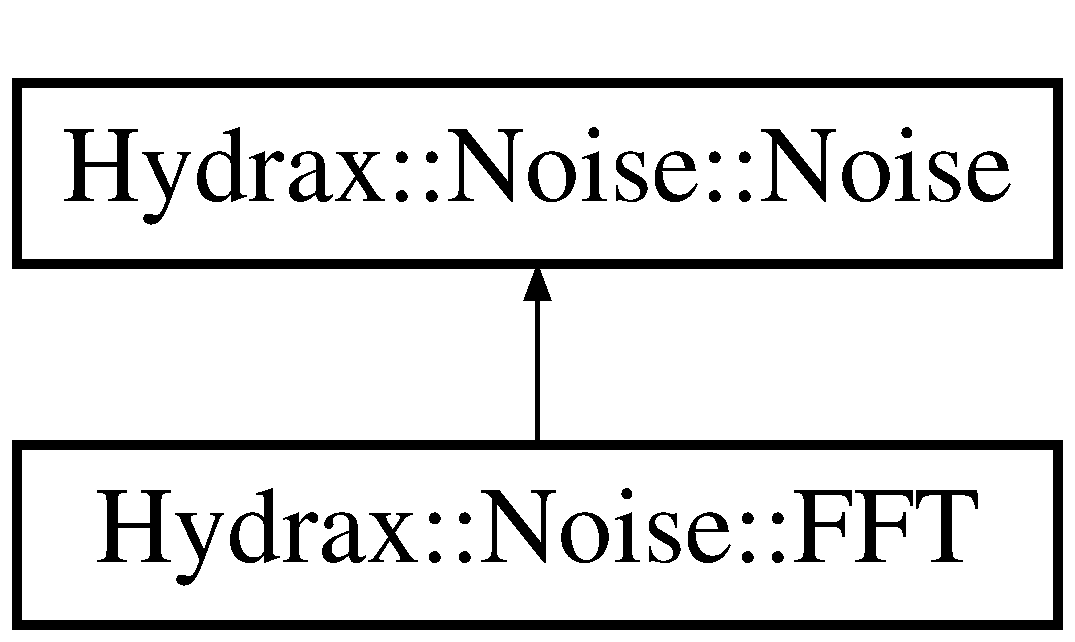
\includegraphics[height=2cm]{class_hydrax_1_1_noise_1_1_f_f_t}
\end{center}
\end{figure}
\subsection*{Classes}
\begin{CompactItemize}
\item 
struct \hyperlink{struct_hydrax_1_1_noise_1_1_f_f_t_1_1_options}{Options}
\end{CompactItemize}
\subsection*{Public Member Functions}
\begin{CompactItemize}
\item 
\hyperlink{class_hydrax_1_1_noise_1_1_f_f_t_5e4f2e1075138aa5255e0f2c90f0e004}{FFT} ()
\item 
\hyperlink{class_hydrax_1_1_noise_1_1_f_f_t_39e0f2bd11f4fcd7afab5a0977446c3e}{FFT} (const \hyperlink{struct_hydrax_1_1_noise_1_1_f_f_t_1_1_options}{Options} \&\hyperlink{struct_hydrax_1_1_noise_1_1_f_f_t_1_1_options}{Options})
\item 
\hyperlink{class_hydrax_1_1_noise_1_1_f_f_t_fd96b8a520f12c10d7cffe16a776034e}{$\sim$FFT} ()
\item 
void \hyperlink{class_hydrax_1_1_noise_1_1_f_f_t_c382e8624b864a32267687592b769bd3}{create} ()
\item 
bool \hyperlink{class_hydrax_1_1_noise_1_1_f_f_t_a8e2b9d2b8307c07be2d2cd9cf115560}{createGPUNormalMapResources} (\hyperlink{class_hydrax_1_1_g_p_u_normal_map_manager}{GPUNormalMapManager} $\ast$g)
\item 
void \hyperlink{class_hydrax_1_1_noise_1_1_f_f_t_9567d90d8fae8dbd74d05d1e3b8281e4}{remove} ()
\item 
void \hyperlink{class_hydrax_1_1_noise_1_1_f_f_t_edb7b8614828cda29b62aa6c1509e22a}{update} (const Ogre::Real \&timeSinceLastFrame)
\item 
void \hyperlink{class_hydrax_1_1_noise_1_1_f_f_t_6e045d4c71f1005305445dbae8701736}{saveCfg} (Ogre::String \&Data)
\item 
bool \hyperlink{class_hydrax_1_1_noise_1_1_f_f_t_64245b9e56eeb8627ac3f5260dc203dd}{loadCfg} (Ogre::ConfigFile \&CfgFile)
\item 
float \hyperlink{class_hydrax_1_1_noise_1_1_f_f_t_e7da5bf6c6ebfc9061ed433af6350ea7}{getValue} (const float \&x, const float \&y)
\item 
void \hyperlink{class_hydrax_1_1_noise_1_1_f_f_t_1d7ec06eb11cda608cc8f73256c35be5}{setOptions} (const \hyperlink{struct_hydrax_1_1_noise_1_1_f_f_t_1_1_options}{Options} \&\hyperlink{struct_hydrax_1_1_noise_1_1_f_f_t_1_1_options}{Options})
\item 
const \hyperlink{struct_hydrax_1_1_noise_1_1_f_f_t_1_1_options}{Options} \& \hyperlink{class_hydrax_1_1_noise_1_1_f_f_t_5207977ba1623fef59570e8f2f1c738c}{getOptions} () const 
\end{CompactItemize}


\subsection{Detailed Description}
\hyperlink{class_hydrax_1_1_noise_1_1_f_f_t}{FFT} noise module class 

\subsection{Constructor \& Destructor Documentation}
\hypertarget{class_hydrax_1_1_noise_1_1_f_f_t_5e4f2e1075138aa5255e0f2c90f0e004}{
\index{Hydrax::Noise::FFT@{Hydrax::Noise::FFT}!FFT@{FFT}}
\index{FFT@{FFT}!Hydrax::Noise::FFT@{Hydrax::Noise::FFT}}
\subsubsection[{FFT}]{\setlength{\rightskip}{0pt plus 5cm}Hydrax::Noise::FFT::FFT ()}}
\label{class_hydrax_1_1_noise_1_1_f_f_t_5e4f2e1075138aa5255e0f2c90f0e004}


Default constructor \hypertarget{class_hydrax_1_1_noise_1_1_f_f_t_39e0f2bd11f4fcd7afab5a0977446c3e}{
\index{Hydrax::Noise::FFT@{Hydrax::Noise::FFT}!FFT@{FFT}}
\index{FFT@{FFT}!Hydrax::Noise::FFT@{Hydrax::Noise::FFT}}
\subsubsection[{FFT}]{\setlength{\rightskip}{0pt plus 5cm}Hydrax::Noise::FFT::FFT (const {\bf Options} \& {\em Options})}}
\label{class_hydrax_1_1_noise_1_1_f_f_t_39e0f2bd11f4fcd7afab5a0977446c3e}


Constructor \begin{Desc}
\item[Parameters:]
\begin{description}
\item[{\em \hyperlink{struct_hydrax_1_1_noise_1_1_f_f_t_1_1_options}{Options}}]\hyperlink{class_hydrax_1_1_noise_1_1_f_f_t}{FFT} noise options \end{description}
\end{Desc}
\hypertarget{class_hydrax_1_1_noise_1_1_f_f_t_fd96b8a520f12c10d7cffe16a776034e}{
\index{Hydrax::Noise::FFT@{Hydrax::Noise::FFT}!$\sim$FFT@{$\sim$FFT}}
\index{$\sim$FFT@{$\sim$FFT}!Hydrax::Noise::FFT@{Hydrax::Noise::FFT}}
\subsubsection[{$\sim$FFT}]{\setlength{\rightskip}{0pt plus 5cm}Hydrax::Noise::FFT::$\sim$FFT ()}}
\label{class_hydrax_1_1_noise_1_1_f_f_t_fd96b8a520f12c10d7cffe16a776034e}


Destructor 

\subsection{Member Function Documentation}
\hypertarget{class_hydrax_1_1_noise_1_1_f_f_t_c382e8624b864a32267687592b769bd3}{
\index{Hydrax::Noise::FFT@{Hydrax::Noise::FFT}!create@{create}}
\index{create@{create}!Hydrax::Noise::FFT@{Hydrax::Noise::FFT}}
\subsubsection[{create}]{\setlength{\rightskip}{0pt plus 5cm}void Hydrax::Noise::FFT::create ()\hspace{0.3cm}{\tt  \mbox{[}virtual\mbox{]}}}}
\label{class_hydrax_1_1_noise_1_1_f_f_t_c382e8624b864a32267687592b769bd3}


Create 

Reimplemented from \hyperlink{class_hydrax_1_1_noise_1_1_noise_be9cf8765feed765e6a35b0779125f6a}{Hydrax::Noise::Noise}.\hypertarget{class_hydrax_1_1_noise_1_1_f_f_t_a8e2b9d2b8307c07be2d2cd9cf115560}{
\index{Hydrax::Noise::FFT@{Hydrax::Noise::FFT}!createGPUNormalMapResources@{createGPUNormalMapResources}}
\index{createGPUNormalMapResources@{createGPUNormalMapResources}!Hydrax::Noise::FFT@{Hydrax::Noise::FFT}}
\subsubsection[{createGPUNormalMapResources}]{\setlength{\rightskip}{0pt plus 5cm}bool Hydrax::Noise::FFT::createGPUNormalMapResources ({\bf GPUNormalMapManager} $\ast$ {\em g})\hspace{0.3cm}{\tt  \mbox{[}virtual\mbox{]}}}}
\label{class_hydrax_1_1_noise_1_1_f_f_t_a8e2b9d2b8307c07be2d2cd9cf115560}


Create GPUNormalMap resources \begin{Desc}
\item[Parameters:]
\begin{description}
\item[{\em g}]\hyperlink{class_hydrax_1_1_g_p_u_normal_map_manager}{GPUNormalMapManager} pointer \end{description}
\end{Desc}
\begin{Desc}
\item[Returns:]true if it needs to be created, false if not \end{Desc}


Reimplemented from \hyperlink{class_hydrax_1_1_noise_1_1_noise_59f0e03e88a5de69065838adc35ff2d8}{Hydrax::Noise::Noise}.\hypertarget{class_hydrax_1_1_noise_1_1_f_f_t_5207977ba1623fef59570e8f2f1c738c}{
\index{Hydrax::Noise::FFT@{Hydrax::Noise::FFT}!getOptions@{getOptions}}
\index{getOptions@{getOptions}!Hydrax::Noise::FFT@{Hydrax::Noise::FFT}}
\subsubsection[{getOptions}]{\setlength{\rightskip}{0pt plus 5cm}const {\bf Options}\& Hydrax::Noise::FFT::getOptions () const\hspace{0.3cm}{\tt  \mbox{[}inline\mbox{]}}}}
\label{class_hydrax_1_1_noise_1_1_f_f_t_5207977ba1623fef59570e8f2f1c738c}


Get current \hyperlink{class_hydrax_1_1_noise_1_1_f_f_t}{FFT} noise options \begin{Desc}
\item[Returns:]Current fft noise options \end{Desc}
\hypertarget{class_hydrax_1_1_noise_1_1_f_f_t_e7da5bf6c6ebfc9061ed433af6350ea7}{
\index{Hydrax::Noise::FFT@{Hydrax::Noise::FFT}!getValue@{getValue}}
\index{getValue@{getValue}!Hydrax::Noise::FFT@{Hydrax::Noise::FFT}}
\subsubsection[{getValue}]{\setlength{\rightskip}{0pt plus 5cm}float Hydrax::Noise::FFT::getValue (const float \& {\em x}, \/  const float \& {\em y})\hspace{0.3cm}{\tt  \mbox{[}virtual\mbox{]}}}}
\label{class_hydrax_1_1_noise_1_1_f_f_t_e7da5bf6c6ebfc9061ed433af6350ea7}


Get the especified x/y noise value \begin{Desc}
\item[Parameters:]
\begin{description}
\item[{\em x}]X Coord \item[{\em y}]Y Coord \end{description}
\end{Desc}
\begin{Desc}
\item[Returns:]\hyperlink{class_hydrax_1_1_noise_1_1_noise}{Noise} value \end{Desc}


Implements \hyperlink{class_hydrax_1_1_noise_1_1_noise_5b18138d5c2c5ea3c3659cef80dd3a3e}{Hydrax::Noise::Noise}.\hypertarget{class_hydrax_1_1_noise_1_1_f_f_t_64245b9e56eeb8627ac3f5260dc203dd}{
\index{Hydrax::Noise::FFT@{Hydrax::Noise::FFT}!loadCfg@{loadCfg}}
\index{loadCfg@{loadCfg}!Hydrax::Noise::FFT@{Hydrax::Noise::FFT}}
\subsubsection[{loadCfg}]{\setlength{\rightskip}{0pt plus 5cm}bool Hydrax::Noise::FFT::loadCfg (Ogre::ConfigFile \& {\em CfgFile})\hspace{0.3cm}{\tt  \mbox{[}virtual\mbox{]}}}}
\label{class_hydrax_1_1_noise_1_1_f_f_t_64245b9e56eeb8627ac3f5260dc203dd}


Load config \begin{Desc}
\item[Parameters:]
\begin{description}
\item[{\em CgfFile}]Ogre::ConfigFile reference \end{description}
\end{Desc}
\begin{Desc}
\item[Returns:]True if is the correct noise config \end{Desc}


Reimplemented from \hyperlink{class_hydrax_1_1_noise_1_1_noise_5ef6e71282a9dfcefc09e3ba84a7578f}{Hydrax::Noise::Noise}.\hypertarget{class_hydrax_1_1_noise_1_1_f_f_t_9567d90d8fae8dbd74d05d1e3b8281e4}{
\index{Hydrax::Noise::FFT@{Hydrax::Noise::FFT}!remove@{remove}}
\index{remove@{remove}!Hydrax::Noise::FFT@{Hydrax::Noise::FFT}}
\subsubsection[{remove}]{\setlength{\rightskip}{0pt plus 5cm}void Hydrax::Noise::FFT::remove ()\hspace{0.3cm}{\tt  \mbox{[}virtual\mbox{]}}}}
\label{class_hydrax_1_1_noise_1_1_f_f_t_9567d90d8fae8dbd74d05d1e3b8281e4}


Remove 

Reimplemented from \hyperlink{class_hydrax_1_1_noise_1_1_noise_00c4aaa7604ea492740318d01f651606}{Hydrax::Noise::Noise}.\hypertarget{class_hydrax_1_1_noise_1_1_f_f_t_6e045d4c71f1005305445dbae8701736}{
\index{Hydrax::Noise::FFT@{Hydrax::Noise::FFT}!saveCfg@{saveCfg}}
\index{saveCfg@{saveCfg}!Hydrax::Noise::FFT@{Hydrax::Noise::FFT}}
\subsubsection[{saveCfg}]{\setlength{\rightskip}{0pt plus 5cm}void Hydrax::Noise::FFT::saveCfg (Ogre::String \& {\em Data})\hspace{0.3cm}{\tt  \mbox{[}virtual\mbox{]}}}}
\label{class_hydrax_1_1_noise_1_1_f_f_t_6e045d4c71f1005305445dbae8701736}


Save config \begin{Desc}
\item[Parameters:]
\begin{description}
\item[{\em Data}]String reference \end{description}
\end{Desc}


Reimplemented from \hyperlink{class_hydrax_1_1_noise_1_1_noise_ac0a9fe1533ddd87467edb954f8abea8}{Hydrax::Noise::Noise}.\hypertarget{class_hydrax_1_1_noise_1_1_f_f_t_1d7ec06eb11cda608cc8f73256c35be5}{
\index{Hydrax::Noise::FFT@{Hydrax::Noise::FFT}!setOptions@{setOptions}}
\index{setOptions@{setOptions}!Hydrax::Noise::FFT@{Hydrax::Noise::FFT}}
\subsubsection[{setOptions}]{\setlength{\rightskip}{0pt plus 5cm}void Hydrax::Noise::FFT::setOptions (const {\bf Options} \& {\em Options})}}
\label{class_hydrax_1_1_noise_1_1_f_f_t_1d7ec06eb11cda608cc8f73256c35be5}


Set/Update fft noise options \begin{Desc}
\item[Parameters:]
\begin{description}
\item[{\em \hyperlink{struct_hydrax_1_1_noise_1_1_f_f_t_1_1_options}{Options}}]\hyperlink{class_hydrax_1_1_noise_1_1_f_f_t}{FFT} noise options \end{description}
\end{Desc}
\hypertarget{class_hydrax_1_1_noise_1_1_f_f_t_edb7b8614828cda29b62aa6c1509e22a}{
\index{Hydrax::Noise::FFT@{Hydrax::Noise::FFT}!update@{update}}
\index{update@{update}!Hydrax::Noise::FFT@{Hydrax::Noise::FFT}}
\subsubsection[{update}]{\setlength{\rightskip}{0pt plus 5cm}void Hydrax::Noise::FFT::update (const Ogre::Real \& {\em timeSinceLastFrame})\hspace{0.3cm}{\tt  \mbox{[}virtual\mbox{]}}}}
\label{class_hydrax_1_1_noise_1_1_f_f_t_edb7b8614828cda29b62aa6c1509e22a}


Call it each frame \begin{Desc}
\item[Parameters:]
\begin{description}
\item[{\em timeSinceLastFrame}]Time since last frame(delta) \end{description}
\end{Desc}


Implements \hyperlink{class_hydrax_1_1_noise_1_1_noise_9c32c4c630f193e034c074f69ea10f57}{Hydrax::Noise::Noise}.

The documentation for this class was generated from the following files:\begin{CompactItemize}
\item 
C:/Hydrax/v0.5.1/Hydrax/src/Hydrax/Noise/FFT/\hyperlink{_f_f_t_8h}{FFT.h}\item 
C:/Hydrax/v0.5.1/Hydrax/src/Hydrax/Noise/FFT/\hyperlink{_f_f_t_8cpp}{FFT.cpp}\end{CompactItemize}

\hypertarget{struct_hydrax_1_1_noise_1_1_f_f_t_1_1_options}{
\section{Hydrax::Noise::FFT::FFT::Options Struct Reference}
\label{struct_hydrax_1_1_noise_1_1_f_f_t_1_1_options}\index{Hydrax::Noise::FFT::Options@{Hydrax::Noise::FFT::Options}}
}
{\tt \#include $<$FFT.h$>$}

\subsection*{Public Member Functions}
\begin{CompactItemize}
\item 
\hyperlink{struct_hydrax_1_1_noise_1_1_f_f_t_1_1_options_177f9a33f992a3ff0895688eaba0fc57}{Options} ()
\item 
\hyperlink{struct_hydrax_1_1_noise_1_1_f_f_t_1_1_options_7c9613db2f0a0a9037c1aaf713bb1d91}{Options} (const int \&\_\-Resolution, const float \&\_\-PhysicalResolution, const float \&\_\-Scale, const Ogre::Vector2 \&\_\-WindDirection, const float \&\_\-AnimationSpeed, const float \&\_\-KwPower, const float \&\_\-Amplitude)
\item 
\hyperlink{struct_hydrax_1_1_noise_1_1_f_f_t_1_1_options_28e1e4f8ce5958e56094139d4f7fd569}{Options} (const int \&\_\-Resolution, const float \&\_\-PhysicalResolution, const float \&\_\-Scale, const Ogre::Vector2 \&\_\-WindDirection, const float \&\_\-AnimationSpeed, const float \&\_\-KwPower, const float \&\_\-Amplitude, const float \&\_\-GPU\_\-Strength, const Ogre::Vector3 \&\_\-GPU\_\-LODParameters)
\end{CompactItemize}
\subsection*{Public Attributes}
\begin{CompactItemize}
\item 
int \hyperlink{struct_hydrax_1_1_noise_1_1_f_f_t_1_1_options_5e7cb0d860838ae205212b13aad05a4b}{Resolution}
\begin{CompactList}\small\item\em \hyperlink{class_hydrax_1_1_noise_1_1_noise}{Noise} resolution (2$^\wedge$n). \item\end{CompactList}\item 
float \hyperlink{struct_hydrax_1_1_noise_1_1_f_f_t_1_1_options_f1273c65d2872198ae6b3c1dfb150ff4}{PhysicalResolution}
\begin{CompactList}\small\item\em Physical resolution. \item\end{CompactList}\item 
float \hyperlink{struct_hydrax_1_1_noise_1_1_f_f_t_1_1_options_98e3899bdfe6bf54910192543fbc374c}{Scale}
\begin{CompactList}\small\item\em \hyperlink{class_hydrax_1_1_noise_1_1_noise}{Noise} scale. \item\end{CompactList}\item 
Ogre::Vector2 \hyperlink{struct_hydrax_1_1_noise_1_1_f_f_t_1_1_options_9ee024e08048211c6674f00d61496037}{WindDirection}
\begin{CompactList}\small\item\em Wind direction. \item\end{CompactList}\item 
float \hyperlink{struct_hydrax_1_1_noise_1_1_f_f_t_1_1_options_87a99bc4e880913e1268cdb8b347998c}{AnimationSpeed}
\begin{CompactList}\small\item\em Animation speed. \item\end{CompactList}\item 
float \hyperlink{struct_hydrax_1_1_noise_1_1_f_f_t_1_1_options_2e3cb6246534f5abdfb23d8d0ce6fa22}{KwPower}
\begin{CompactList}\small\item\em KwPower. \item\end{CompactList}\item 
float \hyperlink{struct_hydrax_1_1_noise_1_1_f_f_t_1_1_options_9e12efef04053de76ba32f2fee4e8296}{Amplitude}
\begin{CompactList}\small\item\em \hyperlink{class_hydrax_1_1_noise_1_1_noise}{Noise} amplitude. \item\end{CompactList}\item 
float \hyperlink{struct_hydrax_1_1_noise_1_1_f_f_t_1_1_options_93cca7338d3a4a201d068e4cd8afa330}{GPU\_\-Strength}
\begin{CompactList}\small\item\em Representes the strength of the normals (i.e. Amplitude). \item\end{CompactList}\item 
Ogre::Vector3 \hyperlink{struct_hydrax_1_1_noise_1_1_f_f_t_1_1_options_407abbd0ee2f841a2856f18aa69d3f98}{GPU\_\-LODParameters}
\end{CompactItemize}


\subsection{Detailed Description}
Struct wich contains fft noise module options 

\subsection{Constructor \& Destructor Documentation}
\hypertarget{struct_hydrax_1_1_noise_1_1_f_f_t_1_1_options_177f9a33f992a3ff0895688eaba0fc57}{
\index{Hydrax::Noise::FFT::Options@{Hydrax::Noise::FFT::Options}!Options@{Options}}
\index{Options@{Options}!Hydrax::Noise::FFT::Options@{Hydrax::Noise::FFT::Options}}
\subsubsection[{Options}]{\setlength{\rightskip}{0pt plus 5cm}Hydrax::Noise::FFT::FFT::Options::Options ()\hspace{0.3cm}{\tt  \mbox{[}inline\mbox{]}}}}
\label{struct_hydrax_1_1_noise_1_1_f_f_t_1_1_options_177f9a33f992a3ff0895688eaba0fc57}


Default constructor \hypertarget{struct_hydrax_1_1_noise_1_1_f_f_t_1_1_options_7c9613db2f0a0a9037c1aaf713bb1d91}{
\index{Hydrax::Noise::FFT::Options@{Hydrax::Noise::FFT::Options}!Options@{Options}}
\index{Options@{Options}!Hydrax::Noise::FFT::Options@{Hydrax::Noise::FFT::Options}}
\subsubsection[{Options}]{\setlength{\rightskip}{0pt plus 5cm}Hydrax::Noise::FFT::FFT::Options::Options (const int \& {\em \_\-Resolution}, \/  const float \& {\em \_\-PhysicalResolution}, \/  const float \& {\em \_\-Scale}, \/  const Ogre::Vector2 \& {\em \_\-WindDirection}, \/  const float \& {\em \_\-AnimationSpeed}, \/  const float \& {\em \_\-KwPower}, \/  const float \& {\em \_\-Amplitude})\hspace{0.3cm}{\tt  \mbox{[}inline\mbox{]}}}}
\label{struct_hydrax_1_1_noise_1_1_f_f_t_1_1_options_7c9613db2f0a0a9037c1aaf713bb1d91}


User constructor \begin{Desc}
\item[Parameters:]
\begin{description}
\item[{\em \_\-Resolution}]\hyperlink{class_hydrax_1_1_noise_1_1_f_f_t}{FFT} Resolution (2$^\wedge$n) \item[{\em \_\-PhysicalResolution}]Physical resolution of the surface \item[{\em \_\-Scale}]\hyperlink{class_hydrax_1_1_noise_1_1_noise}{Noise} scale \item[{\em \_\-WindDirection}]Wind direction \item[{\em \_\-AnimationSpeed}]Animation speed coeficient \item[{\em \_\-KwPower}]KwPower \item[{\em \_\-Amplitude}]\hyperlink{class_hydrax_1_1_noise_1_1_noise}{Noise} amplitude \end{description}
\end{Desc}
\hypertarget{struct_hydrax_1_1_noise_1_1_f_f_t_1_1_options_28e1e4f8ce5958e56094139d4f7fd569}{
\index{Hydrax::Noise::FFT::Options@{Hydrax::Noise::FFT::Options}!Options@{Options}}
\index{Options@{Options}!Hydrax::Noise::FFT::Options@{Hydrax::Noise::FFT::Options}}
\subsubsection[{Options}]{\setlength{\rightskip}{0pt plus 5cm}Hydrax::Noise::FFT::FFT::Options::Options (const int \& {\em \_\-Resolution}, \/  const float \& {\em \_\-PhysicalResolution}, \/  const float \& {\em \_\-Scale}, \/  const Ogre::Vector2 \& {\em \_\-WindDirection}, \/  const float \& {\em \_\-AnimationSpeed}, \/  const float \& {\em \_\-KwPower}, \/  const float \& {\em \_\-Amplitude}, \/  const float \& {\em \_\-GPU\_\-Strength}, \/  const Ogre::Vector3 \& {\em \_\-GPU\_\-LODParameters})\hspace{0.3cm}{\tt  \mbox{[}inline\mbox{]}}}}
\label{struct_hydrax_1_1_noise_1_1_f_f_t_1_1_options_28e1e4f8ce5958e56094139d4f7fd569}


User constructor \begin{Desc}
\item[Parameters:]
\begin{description}
\item[{\em \_\-Resolution}]\hyperlink{class_hydrax_1_1_noise_1_1_f_f_t}{FFT} Resolution (2$^\wedge$n) \item[{\em \_\-PhysicalResolution}]Physical resolution of the surface \item[{\em \_\-Scale}]\hyperlink{class_hydrax_1_1_noise_1_1_noise}{Noise} scale \item[{\em \_\-WindDirection}]Wind direction \item[{\em \_\-AnimationSpeed}]Animation speed coeficient \item[{\em \_\-KwPower}]KwPower \item[{\em \_\-Amplitude}]\hyperlink{class_hydrax_1_1_noise_1_1_noise}{Noise} amplitude \item[{\em \_\-GPU\_\-Strength}]GPU\_\-Strength \item[{\em \_\-GPU\_\-LODParameters}]GPU\_\-LODParameters \end{description}
\end{Desc}


\subsection{Member Data Documentation}
\hypertarget{struct_hydrax_1_1_noise_1_1_f_f_t_1_1_options_9e12efef04053de76ba32f2fee4e8296}{
\index{Hydrax::Noise::FFT::Options@{Hydrax::Noise::FFT::Options}!Amplitude@{Amplitude}}
\index{Amplitude@{Amplitude}!Hydrax::Noise::FFT::Options@{Hydrax::Noise::FFT::Options}}
\subsubsection[{Amplitude}]{\setlength{\rightskip}{0pt plus 5cm}float Hydrax::Noise::FFT::FFT::Options::Amplitude}}
\label{struct_hydrax_1_1_noise_1_1_f_f_t_1_1_options_9e12efef04053de76ba32f2fee4e8296}


\hyperlink{class_hydrax_1_1_noise_1_1_noise}{Noise} amplitude. 

\hypertarget{struct_hydrax_1_1_noise_1_1_f_f_t_1_1_options_87a99bc4e880913e1268cdb8b347998c}{
\index{Hydrax::Noise::FFT::Options@{Hydrax::Noise::FFT::Options}!AnimationSpeed@{AnimationSpeed}}
\index{AnimationSpeed@{AnimationSpeed}!Hydrax::Noise::FFT::Options@{Hydrax::Noise::FFT::Options}}
\subsubsection[{AnimationSpeed}]{\setlength{\rightskip}{0pt plus 5cm}float Hydrax::Noise::FFT::FFT::Options::AnimationSpeed}}
\label{struct_hydrax_1_1_noise_1_1_f_f_t_1_1_options_87a99bc4e880913e1268cdb8b347998c}


Animation speed. 

\hypertarget{struct_hydrax_1_1_noise_1_1_f_f_t_1_1_options_407abbd0ee2f841a2856f18aa69d3f98}{
\index{Hydrax::Noise::FFT::Options@{Hydrax::Noise::FFT::Options}!GPU\_\-LODParameters@{GPU\_\-LODParameters}}
\index{GPU\_\-LODParameters@{GPU\_\-LODParameters}!Hydrax::Noise::FFT::Options@{Hydrax::Noise::FFT::Options}}
\subsubsection[{GPU\_\-LODParameters}]{\setlength{\rightskip}{0pt plus 5cm}Ogre::Vector3 Hydrax::Noise::FFT::FFT::Options::GPU\_\-LODParameters}}
\label{struct_hydrax_1_1_noise_1_1_f_f_t_1_1_options_407abbd0ee2f841a2856f18aa69d3f98}


LOD Parameters, in order to obtain a smooth normal map we need to decrease the detail level when the pixel is far to the camera. This parameters are stored in an Ogre::Vector3: x -$>$ Initial LOD value (Bigger values -$>$ less detail) y -$>$ Final LOD value z -$>$ Final distance \hypertarget{struct_hydrax_1_1_noise_1_1_f_f_t_1_1_options_93cca7338d3a4a201d068e4cd8afa330}{
\index{Hydrax::Noise::FFT::Options@{Hydrax::Noise::FFT::Options}!GPU\_\-Strength@{GPU\_\-Strength}}
\index{GPU\_\-Strength@{GPU\_\-Strength}!Hydrax::Noise::FFT::Options@{Hydrax::Noise::FFT::Options}}
\subsubsection[{GPU\_\-Strength}]{\setlength{\rightskip}{0pt plus 5cm}float Hydrax::Noise::FFT::FFT::Options::GPU\_\-Strength}}
\label{struct_hydrax_1_1_noise_1_1_f_f_t_1_1_options_93cca7338d3a4a201d068e4cd8afa330}


Representes the strength of the normals (i.e. Amplitude). 

GPU Normal map generator parameters Only if GPU normal map generation is active \hypertarget{struct_hydrax_1_1_noise_1_1_f_f_t_1_1_options_2e3cb6246534f5abdfb23d8d0ce6fa22}{
\index{Hydrax::Noise::FFT::Options@{Hydrax::Noise::FFT::Options}!KwPower@{KwPower}}
\index{KwPower@{KwPower}!Hydrax::Noise::FFT::Options@{Hydrax::Noise::FFT::Options}}
\subsubsection[{KwPower}]{\setlength{\rightskip}{0pt plus 5cm}float Hydrax::Noise::FFT::FFT::Options::KwPower}}
\label{struct_hydrax_1_1_noise_1_1_f_f_t_1_1_options_2e3cb6246534f5abdfb23d8d0ce6fa22}


KwPower. 

\hypertarget{struct_hydrax_1_1_noise_1_1_f_f_t_1_1_options_f1273c65d2872198ae6b3c1dfb150ff4}{
\index{Hydrax::Noise::FFT::Options@{Hydrax::Noise::FFT::Options}!PhysicalResolution@{PhysicalResolution}}
\index{PhysicalResolution@{PhysicalResolution}!Hydrax::Noise::FFT::Options@{Hydrax::Noise::FFT::Options}}
\subsubsection[{PhysicalResolution}]{\setlength{\rightskip}{0pt plus 5cm}float Hydrax::Noise::FFT::FFT::Options::PhysicalResolution}}
\label{struct_hydrax_1_1_noise_1_1_f_f_t_1_1_options_f1273c65d2872198ae6b3c1dfb150ff4}


Physical resolution. 

\hypertarget{struct_hydrax_1_1_noise_1_1_f_f_t_1_1_options_5e7cb0d860838ae205212b13aad05a4b}{
\index{Hydrax::Noise::FFT::Options@{Hydrax::Noise::FFT::Options}!Resolution@{Resolution}}
\index{Resolution@{Resolution}!Hydrax::Noise::FFT::Options@{Hydrax::Noise::FFT::Options}}
\subsubsection[{Resolution}]{\setlength{\rightskip}{0pt plus 5cm}int Hydrax::Noise::FFT::FFT::Options::Resolution}}
\label{struct_hydrax_1_1_noise_1_1_f_f_t_1_1_options_5e7cb0d860838ae205212b13aad05a4b}


\hyperlink{class_hydrax_1_1_noise_1_1_noise}{Noise} resolution (2$^\wedge$n). 

\hypertarget{struct_hydrax_1_1_noise_1_1_f_f_t_1_1_options_98e3899bdfe6bf54910192543fbc374c}{
\index{Hydrax::Noise::FFT::Options@{Hydrax::Noise::FFT::Options}!Scale@{Scale}}
\index{Scale@{Scale}!Hydrax::Noise::FFT::Options@{Hydrax::Noise::FFT::Options}}
\subsubsection[{Scale}]{\setlength{\rightskip}{0pt plus 5cm}float Hydrax::Noise::FFT::FFT::Options::Scale}}
\label{struct_hydrax_1_1_noise_1_1_f_f_t_1_1_options_98e3899bdfe6bf54910192543fbc374c}


\hyperlink{class_hydrax_1_1_noise_1_1_noise}{Noise} scale. 

\hypertarget{struct_hydrax_1_1_noise_1_1_f_f_t_1_1_options_9ee024e08048211c6674f00d61496037}{
\index{Hydrax::Noise::FFT::Options@{Hydrax::Noise::FFT::Options}!WindDirection@{WindDirection}}
\index{WindDirection@{WindDirection}!Hydrax::Noise::FFT::Options@{Hydrax::Noise::FFT::Options}}
\subsubsection[{WindDirection}]{\setlength{\rightskip}{0pt plus 5cm}Ogre::Vector2 Hydrax::Noise::FFT::FFT::Options::WindDirection}}
\label{struct_hydrax_1_1_noise_1_1_f_f_t_1_1_options_9ee024e08048211c6674f00d61496037}


Wind direction. 



The documentation for this struct was generated from the following file:\begin{CompactItemize}
\item 
C:/Hydrax/v0.5.1/Hydrax/src/Hydrax/Noise/FFT/\hyperlink{_f_f_t_8h}{FFT.h}\end{CompactItemize}

\hypertarget{class_hydrax_1_1_god_rays_manager}{
\section{Hydrax::GodRaysManager Class Reference}
\label{class_hydrax_1_1_god_rays_manager}\index{Hydrax::GodRaysManager@{Hydrax::GodRaysManager}}
}
{\tt \#include $<$GodRaysManager.h$>$}

\subsection*{Classes}
\begin{CompactItemize}
\item 
class \textbf{DepthMapListener}
\end{CompactItemize}
\subsection*{Public Types}
\begin{CompactItemize}
\item 
enum \hyperlink{class_hydrax_1_1_god_rays_manager_88654235c3d8c74a152a8b81b9a419cb}{MaterialType} \{ \hyperlink{class_hydrax_1_1_god_rays_manager_88654235c3d8c74a152a8b81b9a419cbc48ce8001d4a4963cbb2b7ef37dd24dc}{MAT\_\-GODRAYS} =  0, 
\hyperlink{class_hydrax_1_1_god_rays_manager_88654235c3d8c74a152a8b81b9a419cbd4f1fac272fd8b2ec734eeacc3c6bfbd}{MAT\_\-DEPTH} =  1
 \}
\subsection*{Public Member Functions}
\begin{CompactItemize}
\item 
\hyperlink{class_hydrax_1_1_god_rays_manager_f655dc90ddc7963fcdbbe567bc2c2f7a}{GodRaysManager} (\hyperlink{class_hydrax_1_1_hydrax}{Hydrax} $\ast$h)
\item 
\hyperlink{class_hydrax_1_1_god_rays_manager_6c76b08ac42e38a3621eac4f71d7f3ae}{$\sim$GodRaysManager} ()
\item 
void \hyperlink{class_hydrax_1_1_god_rays_manager_d6e8cfa4b9bde36b668d04ae3cfe8d00}{create} (const \hyperlink{namespace_hydrax_e8e15abf83a51b0cf514c7d1a133650a}{HydraxComponent} \&HC)
\item 
void \hyperlink{class_hydrax_1_1_god_rays_manager_c4f9cdb2271b323d518c7bc84e3bf2da}{remove} ()
\item 
void \hyperlink{class_hydrax_1_1_god_rays_manager_90ec2ead8e869ab4388641de1edeba11}{update} (const Ogre::Real \&timeSinceLastFrame)
\item 
const bool \& \hyperlink{class_hydrax_1_1_god_rays_manager_2843f0e85cd38ccd93c43698cfddae21}{isCreated} () const 
\item 
void \hyperlink{class_hydrax_1_1_god_rays_manager_be86da8a21691f1bac9d817147c9edba}{addDepthTechnique} (Ogre::Technique $\ast$Technique, const bool \&AutoUpdate=true)
\item 
void \hyperlink{class_hydrax_1_1_god_rays_manager_b8080a305138ef10e0f18f9037f99a8d}{setSimulationSpeed} (const Ogre::Real \&Speed)
\item 
const Ogre::Real \& \hyperlink{class_hydrax_1_1_god_rays_manager_707a5affb30167956b5d7d0696633ac2}{getSimulationSpeed} () const 
\item 
void \hyperlink{class_hydrax_1_1_god_rays_manager_ed0d897dae3ae6c585a616d071f02c71}{setNumberOfRays} (const int \&NumberOfRays)
\item 
const int \& \hyperlink{class_hydrax_1_1_god_rays_manager_b3f75e765c4b537d0c8162591edae631}{getNumberOfRays} () const 
\item 
void \hyperlink{class_hydrax_1_1_god_rays_manager_92f0cf78d74335694d7e81b23e654ee7}{setRaysSize} (const Ogre::Real \&\hyperlink{struct_hydrax_1_1_size}{Size})
\item 
const Ogre::Real \& \hyperlink{class_hydrax_1_1_god_rays_manager_80a4d001a4fd540a73cdbded89660c8d}{getRaysSize} () const 
\item 
\hyperlink{class_hydrax_1_1_noise_1_1_perlin}{Noise::Perlin} $\ast$ \hyperlink{class_hydrax_1_1_god_rays_manager_90d9d1c53fc66eae89e4334580cd73bb}{getPerlin} ()
\item 
Ogre::SceneNode $\ast$ \hyperlink{class_hydrax_1_1_god_rays_manager_9b94205d807dc98568fe5161a0bbc6d7}{getSceneNode} ()
\item 
void \hyperlink{class_hydrax_1_1_god_rays_manager_1cf1f1ec683484ee6949a32bb4fe0e62}{setVisible} (const bool \&Visible)
\item 
const bool \hyperlink{class_hydrax_1_1_god_rays_manager_b58ff59d51808f29ad9108870200d264}{isVisible} () const 
\item 
void \hyperlink{class_hydrax_1_1_god_rays_manager_4a85152f7e71a50c473ae65b299f3465}{setObjectIntersectionsEnabled} (const bool \&Enable)
\item 
const bool \& \hyperlink{class_hydrax_1_1_god_rays_manager_e150748f9126fee118cf9262b76db170}{areObjectsIntersectionsEnabled} () const 
\item 
const Ogre::Vector4 \hyperlink{class_hydrax_1_1_god_rays_manager_cbbe97591ed2ce41ff2791c00588823d}{getNoiseParameters} () const 
\item 
void \hyperlink{class_hydrax_1_1_god_rays_manager_7ca2848326fa661d5a62a830b108be38}{setNoiseParameters} (Ogre::Vector4 Params)
\end{CompactItemize}


\subsection{Detailed Description}
Underwater god rays manager class God rays 

\subsection{Member Enumeration Documentation}
\hypertarget{class_hydrax_1_1_god_rays_manager_88654235c3d8c74a152a8b81b9a419cb}{
\index{Hydrax::GodRaysManager@{Hydrax::GodRaysManager}!MaterialType@{MaterialType}}
\index{MaterialType@{MaterialType}!Hydrax::GodRaysManager@{Hydrax::GodRaysManager}}
\subsubsection[{MaterialType}]{\setlength{\rightskip}{0pt plus 5cm}enum {\bf Hydrax::GodRaysManager::MaterialType}}}
\label{class_hydrax_1_1_god_rays_manager_88654235c3d8c74a152a8b81b9a419cb}


God rays material enumeration \begin{Desc}
\item[Enumerator: ]\par
\begin{description}
\index{MAT\_\-GODRAYS@{MAT\_\-GODRAYS}!Hydrax::GodRaysManager@{Hydrax::GodRaysManager}}\index{Hydrax::GodRaysManager@{Hydrax::GodRaysManager}!MAT\_\-GODRAYS@{MAT\_\-GODRAYS}}\item[{\em 
\hypertarget{class_hydrax_1_1_god_rays_manager_88654235c3d8c74a152a8b81b9a419cbc48ce8001d4a4963cbb2b7ef37dd24dc}{
MAT\_\-GODRAYS}
\label{class_hydrax_1_1_god_rays_manager_88654235c3d8c74a152a8b81b9a419cbc48ce8001d4a4963cbb2b7ef37dd24dc}
}]\index{MAT\_\-DEPTH@{MAT\_\-DEPTH}!Hydrax::GodRaysManager@{Hydrax::GodRaysManager}}\index{Hydrax::GodRaysManager@{Hydrax::GodRaysManager}!MAT\_\-DEPTH@{MAT\_\-DEPTH}}\item[{\em 
\hypertarget{class_hydrax_1_1_god_rays_manager_88654235c3d8c74a152a8b81b9a419cbd4f1fac272fd8b2ec734eeacc3c6bfbd}{
MAT\_\-DEPTH}
\label{class_hydrax_1_1_god_rays_manager_88654235c3d8c74a152a8b81b9a419cbd4f1fac272fd8b2ec734eeacc3c6bfbd}
}]\end{description}
\end{Desc}



\subsection{Constructor \& Destructor Documentation}
\hypertarget{class_hydrax_1_1_god_rays_manager_f655dc90ddc7963fcdbbe567bc2c2f7a}{
\index{Hydrax::GodRaysManager@{Hydrax::GodRaysManager}!GodRaysManager@{GodRaysManager}}
\index{GodRaysManager@{GodRaysManager}!Hydrax::GodRaysManager@{Hydrax::GodRaysManager}}
\subsubsection[{GodRaysManager}]{\setlength{\rightskip}{0pt plus 5cm}Hydrax::GodRaysManager::GodRaysManager ({\bf Hydrax} $\ast$ {\em h})}}
\label{class_hydrax_1_1_god_rays_manager_f655dc90ddc7963fcdbbe567bc2c2f7a}


Constructor \begin{Desc}
\item[Parameters:]
\begin{description}
\item[{\em h}]\hyperlink{class_hydrax_1_1_hydrax}{Hydrax} parent pointer \end{description}
\end{Desc}
\hypertarget{class_hydrax_1_1_god_rays_manager_6c76b08ac42e38a3621eac4f71d7f3ae}{
\index{Hydrax::GodRaysManager@{Hydrax::GodRaysManager}!$\sim$GodRaysManager@{$\sim$GodRaysManager}}
\index{$\sim$GodRaysManager@{$\sim$GodRaysManager}!Hydrax::GodRaysManager@{Hydrax::GodRaysManager}}
\subsubsection[{$\sim$GodRaysManager}]{\setlength{\rightskip}{0pt plus 5cm}Hydrax::GodRaysManager::$\sim$GodRaysManager ()}}
\label{class_hydrax_1_1_god_rays_manager_6c76b08ac42e38a3621eac4f71d7f3ae}


Destructor 

\subsection{Member Function Documentation}
\hypertarget{class_hydrax_1_1_god_rays_manager_be86da8a21691f1bac9d817147c9edba}{
\index{Hydrax::GodRaysManager@{Hydrax::GodRaysManager}!addDepthTechnique@{addDepthTechnique}}
\index{addDepthTechnique@{addDepthTechnique}!Hydrax::GodRaysManager@{Hydrax::GodRaysManager}}
\subsubsection[{addDepthTechnique}]{\setlength{\rightskip}{0pt plus 5cm}void Hydrax::GodRaysManager::addDepthTechnique (Ogre::Technique $\ast$ {\em Technique}, \/  const bool \& {\em AutoUpdate} = {\tt true})}}
\label{class_hydrax_1_1_god_rays_manager_be86da8a21691f1bac9d817147c9edba}


Add god rays depth technique to an especified material \begin{Desc}
\item[Parameters:]
\begin{description}
\item[{\em Technique}]Technique where depth technique will be added \item[{\em AutoUpdate}]The technique will be automatically updated when god rays parameters change \end{description}
\end{Desc}
\begin{Desc}
\item[Remarks:]Call it after \hyperlink{class_hydrax_1_1_hydrax_af840e19208614533a6b344e32965ee2}{Hydrax::create()}/HydraxsetComponents(...)\end{Desc}
The technique will be automatically updated when god rays parameters change if parameter AutoUpdate == true Add depth technique when a material is not an Ogre::Entity, such terrains, PLSM2 materials, etc. This depth technique will be added with \char`\"{}HydraxGodRaysDepth\char`\"{} scheme in ordeto can use it in the G.R. depth RTT. \hypertarget{class_hydrax_1_1_god_rays_manager_e150748f9126fee118cf9262b76db170}{
\index{Hydrax::GodRaysManager@{Hydrax::GodRaysManager}!areObjectsIntersectionsEnabled@{areObjectsIntersectionsEnabled}}
\index{areObjectsIntersectionsEnabled@{areObjectsIntersectionsEnabled}!Hydrax::GodRaysManager@{Hydrax::GodRaysManager}}
\subsubsection[{areObjectsIntersectionsEnabled}]{\setlength{\rightskip}{0pt plus 5cm}const bool\& Hydrax::GodRaysManager::areObjectsIntersectionsEnabled () const\hspace{0.3cm}{\tt  \mbox{[}inline\mbox{]}}}}
\label{class_hydrax_1_1_god_rays_manager_e150748f9126fee118cf9262b76db170}


Are rays objects intersections enabled? \begin{Desc}
\item[Returns:]true if yes, false if not \end{Desc}
\hypertarget{class_hydrax_1_1_god_rays_manager_d6e8cfa4b9bde36b668d04ae3cfe8d00}{
\index{Hydrax::GodRaysManager@{Hydrax::GodRaysManager}!create@{create}}
\index{create@{create}!Hydrax::GodRaysManager@{Hydrax::GodRaysManager}}
\subsubsection[{create}]{\setlength{\rightskip}{0pt plus 5cm}void Hydrax::GodRaysManager::create (const {\bf HydraxComponent} \& {\em HC})}}
\label{class_hydrax_1_1_god_rays_manager_d6e8cfa4b9bde36b668d04ae3cfe8d00}


Create  Current \hyperlink{class_hydrax_1_1_hydrax}{Hydrax} components \hypertarget{class_hydrax_1_1_god_rays_manager_cbbe97591ed2ce41ff2791c00588823d}{
\index{Hydrax::GodRaysManager@{Hydrax::GodRaysManager}!getNoiseParameters@{getNoiseParameters}}
\index{getNoiseParameters@{getNoiseParameters}!Hydrax::GodRaysManager@{Hydrax::GodRaysManager}}
\subsubsection[{getNoiseParameters}]{\setlength{\rightskip}{0pt plus 5cm}const Ogre::Vector4 Hydrax::GodRaysManager::getNoiseParameters () const\hspace{0.3cm}{\tt  \mbox{[}inline\mbox{]}}}}
\label{class_hydrax_1_1_god_rays_manager_cbbe97591ed2ce41ff2791c00588823d}


Get noise params \begin{Desc}
\item[Returns:]Ogre::Vector4 that stores 4 parameters: x-$>$ \hyperlink{namespace_hydrax_1_1_noise}{Noise} derivation y-$>$ Position multiplier z-$>$ Y normal component multiplier w-$>$ Normal multiplier \end{Desc}
\hypertarget{class_hydrax_1_1_god_rays_manager_b3f75e765c4b537d0c8162591edae631}{
\index{Hydrax::GodRaysManager@{Hydrax::GodRaysManager}!getNumberOfRays@{getNumberOfRays}}
\index{getNumberOfRays@{getNumberOfRays}!Hydrax::GodRaysManager@{Hydrax::GodRaysManager}}
\subsubsection[{getNumberOfRays}]{\setlength{\rightskip}{0pt plus 5cm}const int\& Hydrax::GodRaysManager::getNumberOfRays () const\hspace{0.3cm}{\tt  \mbox{[}inline\mbox{]}}}}
\label{class_hydrax_1_1_god_rays_manager_b3f75e765c4b537d0c8162591edae631}


Get number of god rays \begin{Desc}
\item[Returns:]Number of god rays \end{Desc}
\hypertarget{class_hydrax_1_1_god_rays_manager_90d9d1c53fc66eae89e4334580cd73bb}{
\index{Hydrax::GodRaysManager@{Hydrax::GodRaysManager}!getPerlin@{getPerlin}}
\index{getPerlin@{getPerlin}!Hydrax::GodRaysManager@{Hydrax::GodRaysManager}}
\subsubsection[{getPerlin}]{\setlength{\rightskip}{0pt plus 5cm}{\bf Noise::Perlin}$\ast$ Hydrax::GodRaysManager::getPerlin ()\hspace{0.3cm}{\tt  \mbox{[}inline\mbox{]}}}}
\label{class_hydrax_1_1_god_rays_manager_90d9d1c53fc66eae89e4334580cd73bb}


Get perlin noise module \begin{Desc}
\item[Returns:]Perlin noise module \end{Desc}
\hypertarget{class_hydrax_1_1_god_rays_manager_80a4d001a4fd540a73cdbded89660c8d}{
\index{Hydrax::GodRaysManager@{Hydrax::GodRaysManager}!getRaysSize@{getRaysSize}}
\index{getRaysSize@{getRaysSize}!Hydrax::GodRaysManager@{Hydrax::GodRaysManager}}
\subsubsection[{getRaysSize}]{\setlength{\rightskip}{0pt plus 5cm}const Ogre::Real\& Hydrax::GodRaysManager::getRaysSize () const\hspace{0.3cm}{\tt  \mbox{[}inline\mbox{]}}}}
\label{class_hydrax_1_1_god_rays_manager_80a4d001a4fd540a73cdbded89660c8d}


Get god rays size \begin{Desc}
\item[Returns:]Rays size \end{Desc}
\hypertarget{class_hydrax_1_1_god_rays_manager_9b94205d807dc98568fe5161a0bbc6d7}{
\index{Hydrax::GodRaysManager@{Hydrax::GodRaysManager}!getSceneNode@{getSceneNode}}
\index{getSceneNode@{getSceneNode}!Hydrax::GodRaysManager@{Hydrax::GodRaysManager}}
\subsubsection[{getSceneNode}]{\setlength{\rightskip}{0pt plus 5cm}Ogre::SceneNode$\ast$ Hydrax::GodRaysManager::getSceneNode ()\hspace{0.3cm}{\tt  \mbox{[}inline\mbox{]}}}}
\label{class_hydrax_1_1_god_rays_manager_9b94205d807dc98568fe5161a0bbc6d7}


Get good rays scene node \begin{Desc}
\item[Returns:]God rays scene node \end{Desc}
\hypertarget{class_hydrax_1_1_god_rays_manager_707a5affb30167956b5d7d0696633ac2}{
\index{Hydrax::GodRaysManager@{Hydrax::GodRaysManager}!getSimulationSpeed@{getSimulationSpeed}}
\index{getSimulationSpeed@{getSimulationSpeed}!Hydrax::GodRaysManager@{Hydrax::GodRaysManager}}
\subsubsection[{getSimulationSpeed}]{\setlength{\rightskip}{0pt plus 5cm}const Ogre::Real\& Hydrax::GodRaysManager::getSimulationSpeed () const\hspace{0.3cm}{\tt  \mbox{[}inline\mbox{]}}}}
\label{class_hydrax_1_1_god_rays_manager_707a5affb30167956b5d7d0696633ac2}


Get god rays simulation speed \begin{Desc}
\item[Returns:]Simlation speed \end{Desc}
\hypertarget{class_hydrax_1_1_god_rays_manager_2843f0e85cd38ccd93c43698cfddae21}{
\index{Hydrax::GodRaysManager@{Hydrax::GodRaysManager}!isCreated@{isCreated}}
\index{isCreated@{isCreated}!Hydrax::GodRaysManager@{Hydrax::GodRaysManager}}
\subsubsection[{isCreated}]{\setlength{\rightskip}{0pt plus 5cm}const bool\& Hydrax::GodRaysManager::isCreated () const\hspace{0.3cm}{\tt  \mbox{[}inline\mbox{]}}}}
\label{class_hydrax_1_1_god_rays_manager_2843f0e85cd38ccd93c43698cfddae21}


Has been \hyperlink{class_hydrax_1_1_god_rays_manager_d6e8cfa4b9bde36b668d04ae3cfe8d00}{create()} already called? \begin{Desc}
\item[Returns:]true If yes \end{Desc}
\hypertarget{class_hydrax_1_1_god_rays_manager_b58ff59d51808f29ad9108870200d264}{
\index{Hydrax::GodRaysManager@{Hydrax::GodRaysManager}!isVisible@{isVisible}}
\index{isVisible@{isVisible}!Hydrax::GodRaysManager@{Hydrax::GodRaysManager}}
\subsubsection[{isVisible}]{\setlength{\rightskip}{0pt plus 5cm}const bool Hydrax::GodRaysManager::isVisible () const\hspace{0.3cm}{\tt  \mbox{[}inline\mbox{]}}}}
\label{class_hydrax_1_1_god_rays_manager_b58ff59d51808f29ad9108870200d264}


Is visible? \begin{Desc}
\item[Returns:]true if it's visible, false if not \end{Desc}
\hypertarget{class_hydrax_1_1_god_rays_manager_c4f9cdb2271b323d518c7bc84e3bf2da}{
\index{Hydrax::GodRaysManager@{Hydrax::GodRaysManager}!remove@{remove}}
\index{remove@{remove}!Hydrax::GodRaysManager@{Hydrax::GodRaysManager}}
\subsubsection[{remove}]{\setlength{\rightskip}{0pt plus 5cm}void Hydrax::GodRaysManager::remove ()}}
\label{class_hydrax_1_1_god_rays_manager_c4f9cdb2271b323d518c7bc84e3bf2da}


Remove \hypertarget{class_hydrax_1_1_god_rays_manager_7ca2848326fa661d5a62a830b108be38}{
\index{Hydrax::GodRaysManager@{Hydrax::GodRaysManager}!setNoiseParameters@{setNoiseParameters}}
\index{setNoiseParameters@{setNoiseParameters}!Hydrax::GodRaysManager@{Hydrax::GodRaysManager}}
\subsubsection[{setNoiseParameters}]{\setlength{\rightskip}{0pt plus 5cm}void Hydrax::GodRaysManager::setNoiseParameters (Ogre::Vector4 {\em Params})\hspace{0.3cm}{\tt  \mbox{[}inline\mbox{]}}}}
\label{class_hydrax_1_1_god_rays_manager_7ca2848326fa661d5a62a830b108be38}


Set noise params \begin{Desc}
\item[Parameters:]
\begin{description}
\item[{\em Params,:}]x-$>$ \hyperlink{namespace_hydrax_1_1_noise}{Noise} derivation y-$>$ Position multiplier z-$>$ Y normal component multiplier w-$>$ Normal multiplier \end{description}
\end{Desc}
\hypertarget{class_hydrax_1_1_god_rays_manager_ed0d897dae3ae6c585a616d071f02c71}{
\index{Hydrax::GodRaysManager@{Hydrax::GodRaysManager}!setNumberOfRays@{setNumberOfRays}}
\index{setNumberOfRays@{setNumberOfRays}!Hydrax::GodRaysManager@{Hydrax::GodRaysManager}}
\subsubsection[{setNumberOfRays}]{\setlength{\rightskip}{0pt plus 5cm}void Hydrax::GodRaysManager::setNumberOfRays (const int \& {\em NumberOfRays})}}
\label{class_hydrax_1_1_god_rays_manager_ed0d897dae3ae6c585a616d071f02c71}


Set the number of god rays \begin{Desc}
\item[Parameters:]
\begin{description}
\item[{\em NumberOfRays}]Number of god rays \end{description}
\end{Desc}
\hypertarget{class_hydrax_1_1_god_rays_manager_4a85152f7e71a50c473ae65b299f3465}{
\index{Hydrax::GodRaysManager@{Hydrax::GodRaysManager}!setObjectIntersectionsEnabled@{setObjectIntersectionsEnabled}}
\index{setObjectIntersectionsEnabled@{setObjectIntersectionsEnabled}!Hydrax::GodRaysManager@{Hydrax::GodRaysManager}}
\subsubsection[{setObjectIntersectionsEnabled}]{\setlength{\rightskip}{0pt plus 5cm}void Hydrax::GodRaysManager::setObjectIntersectionsEnabled (const bool \& {\em Enable})}}
\label{class_hydrax_1_1_god_rays_manager_4a85152f7e71a50c473ae65b299f3465}


Set objects intersections enabled \begin{Desc}
\item[Parameters:]
\begin{description}
\item[{\em Enable}]true for yes, false for not \end{description}
\end{Desc}
\hypertarget{class_hydrax_1_1_god_rays_manager_92f0cf78d74335694d7e81b23e654ee7}{
\index{Hydrax::GodRaysManager@{Hydrax::GodRaysManager}!setRaysSize@{setRaysSize}}
\index{setRaysSize@{setRaysSize}!Hydrax::GodRaysManager@{Hydrax::GodRaysManager}}
\subsubsection[{setRaysSize}]{\setlength{\rightskip}{0pt plus 5cm}void Hydrax::GodRaysManager::setRaysSize (const Ogre::Real \& {\em Size})\hspace{0.3cm}{\tt  \mbox{[}inline\mbox{]}}}}
\label{class_hydrax_1_1_god_rays_manager_92f0cf78d74335694d7e81b23e654ee7}


Set god rays size \begin{Desc}
\item[Parameters:]
\begin{description}
\item[{\em \hyperlink{struct_hydrax_1_1_size}{Size}}]God rays size \end{description}
\end{Desc}
\hypertarget{class_hydrax_1_1_god_rays_manager_b8080a305138ef10e0f18f9037f99a8d}{
\index{Hydrax::GodRaysManager@{Hydrax::GodRaysManager}!setSimulationSpeed@{setSimulationSpeed}}
\index{setSimulationSpeed@{setSimulationSpeed}!Hydrax::GodRaysManager@{Hydrax::GodRaysManager}}
\subsubsection[{setSimulationSpeed}]{\setlength{\rightskip}{0pt plus 5cm}void Hydrax::GodRaysManager::setSimulationSpeed (const Ogre::Real \& {\em Speed})\hspace{0.3cm}{\tt  \mbox{[}inline\mbox{]}}}}
\label{class_hydrax_1_1_god_rays_manager_b8080a305138ef10e0f18f9037f99a8d}


Set god rays simulation speed \begin{Desc}
\item[Parameters:]
\begin{description}
\item[{\em Speed}]Simulation speed \end{description}
\end{Desc}
\hypertarget{class_hydrax_1_1_god_rays_manager_1cf1f1ec683484ee6949a32bb4fe0e62}{
\index{Hydrax::GodRaysManager@{Hydrax::GodRaysManager}!setVisible@{setVisible}}
\index{setVisible@{setVisible}!Hydrax::GodRaysManager@{Hydrax::GodRaysManager}}
\subsubsection[{setVisible}]{\setlength{\rightskip}{0pt plus 5cm}void Hydrax::GodRaysManager::setVisible (const bool \& {\em Visible})\hspace{0.3cm}{\tt  \mbox{[}inline\mbox{]}}}}
\label{class_hydrax_1_1_god_rays_manager_1cf1f1ec683484ee6949a32bb4fe0e62}


Set visible \begin{Desc}
\item[Parameters:]
\begin{description}
\item[{\em Visible}]true = yes; false = no \end{description}
\end{Desc}
\hypertarget{class_hydrax_1_1_god_rays_manager_90ec2ead8e869ab4388641de1edeba11}{
\index{Hydrax::GodRaysManager@{Hydrax::GodRaysManager}!update@{update}}
\index{update@{update}!Hydrax::GodRaysManager@{Hydrax::GodRaysManager}}
\subsubsection[{update}]{\setlength{\rightskip}{0pt plus 5cm}void Hydrax::GodRaysManager::update (const Ogre::Real \& {\em timeSinceLastFrame})}}
\label{class_hydrax_1_1_god_rays_manager_90ec2ead8e869ab4388641de1edeba11}


Call each frame \begin{Desc}
\item[Parameters:]
\begin{description}
\item[{\em timeSinceLastFrame}]Time since last frame \end{description}
\end{Desc}


The documentation for this class was generated from the following files:\begin{CompactItemize}
\item 
C:/Hydrax/v0.5.1/Hydrax/src/Hydrax/\hyperlink{_god_rays_manager_8h}{GodRaysManager.h}\item 
C:/Hydrax/v0.5.1/Hydrax/src/Hydrax/\hyperlink{_god_rays_manager_8cpp}{GodRaysManager.cpp}\end{CompactItemize}

\hypertarget{class_hydrax_1_1_g_p_u_normal_map_manager}{
\section{Hydrax::GPUNormalMapManager Class Reference}
\label{class_hydrax_1_1_g_p_u_normal_map_manager}\index{Hydrax::GPUNormalMapManager@{Hydrax::GPUNormalMapManager}}
}
{\tt \#include $<$GPUNormalMapManager.h$>$}

\subsection*{Public Member Functions}
\begin{CompactItemize}
\item 
\hyperlink{class_hydrax_1_1_g_p_u_normal_map_manager_9c2a79cec8c9a72e2916587e09c9c83f}{GPUNormalMapManager} (\hyperlink{class_hydrax_1_1_hydrax}{Hydrax} $\ast$h)
\item 
\hyperlink{class_hydrax_1_1_g_p_u_normal_map_manager_00de9b3c181b8b91e1a8448f4e70976c}{$\sim$GPUNormalMapManager} ()
\item 
void \hyperlink{class_hydrax_1_1_g_p_u_normal_map_manager_7398a504e11ea902839868d69bcf956b}{create} ()
\item 
void \hyperlink{class_hydrax_1_1_g_p_u_normal_map_manager_3a9a24e5832aaa24f78025d1ba04f8a3}{remove} ()
\item 
void \hyperlink{class_hydrax_1_1_g_p_u_normal_map_manager_c58c786ad6359d8f70b5ecd0bc30464b}{setActive} (const bool \&Active)
\item 
const bool \& \hyperlink{class_hydrax_1_1_g_p_u_normal_map_manager_08b3f31fd1b4be43a6f0cc8ac0063077}{isCreated} () const 
\item 
\hyperlink{class_hydrax_1_1_hydrax}{Hydrax} $\ast$ \hyperlink{class_hydrax_1_1_g_p_u_normal_map_manager_8252b201663431e9760cf1e9586afc81}{getHydrax} ()
\item 
Ogre::MaterialPtr \& \hyperlink{class_hydrax_1_1_g_p_u_normal_map_manager_03dbe50e39daea6c40ac192c0afa1936}{getNormalMapMaterial} ()
\item 
Ogre::TexturePtr \& \hyperlink{class_hydrax_1_1_g_p_u_normal_map_manager_b37c3778df109d139c6136fbda3abe80}{getTexture} (const int \&Index)
\item 
void \hyperlink{class_hydrax_1_1_g_p_u_normal_map_manager_6f1b8618e5a860bbd1300c5beedf1194}{addTexture} (Ogre::TexturePtr \&Texture)
\item 
void \hyperlink{class_hydrax_1_1_g_p_u_normal_map_manager_134fe8bf7ebfbcf75e3a7953a5beb028}{removeTexture} (const int \&Index)
\end{CompactItemize}


\subsection{Detailed Description}
Class to manager GPU normal maps 

\subsection{Constructor \& Destructor Documentation}
\hypertarget{class_hydrax_1_1_g_p_u_normal_map_manager_9c2a79cec8c9a72e2916587e09c9c83f}{
\index{Hydrax::GPUNormalMapManager@{Hydrax::GPUNormalMapManager}!GPUNormalMapManager@{GPUNormalMapManager}}
\index{GPUNormalMapManager@{GPUNormalMapManager}!Hydrax::GPUNormalMapManager@{Hydrax::GPUNormalMapManager}}
\subsubsection[{GPUNormalMapManager}]{\setlength{\rightskip}{0pt plus 5cm}Hydrax::GPUNormalMapManager::GPUNormalMapManager ({\bf Hydrax} $\ast$ {\em h})}}
\label{class_hydrax_1_1_g_p_u_normal_map_manager_9c2a79cec8c9a72e2916587e09c9c83f}


Constructor \begin{Desc}
\item[Parameters:]
\begin{description}
\item[{\em h}]\hyperlink{class_hydrax_1_1_hydrax}{Hydrax} main pointer \end{description}
\end{Desc}
\hypertarget{class_hydrax_1_1_g_p_u_normal_map_manager_00de9b3c181b8b91e1a8448f4e70976c}{
\index{Hydrax::GPUNormalMapManager@{Hydrax::GPUNormalMapManager}!$\sim$GPUNormalMapManager@{$\sim$GPUNormalMapManager}}
\index{$\sim$GPUNormalMapManager@{$\sim$GPUNormalMapManager}!Hydrax::GPUNormalMapManager@{Hydrax::GPUNormalMapManager}}
\subsubsection[{$\sim$GPUNormalMapManager}]{\setlength{\rightskip}{0pt plus 5cm}Hydrax::GPUNormalMapManager::$\sim$GPUNormalMapManager ()}}
\label{class_hydrax_1_1_g_p_u_normal_map_manager_00de9b3c181b8b91e1a8448f4e70976c}


Destructor 

\subsection{Member Function Documentation}
\hypertarget{class_hydrax_1_1_g_p_u_normal_map_manager_6f1b8618e5a860bbd1300c5beedf1194}{
\index{Hydrax::GPUNormalMapManager@{Hydrax::GPUNormalMapManager}!addTexture@{addTexture}}
\index{addTexture@{addTexture}!Hydrax::GPUNormalMapManager@{Hydrax::GPUNormalMapManager}}
\subsubsection[{addTexture}]{\setlength{\rightskip}{0pt plus 5cm}void Hydrax::GPUNormalMapManager::addTexture (Ogre::TexturePtr \& {\em Texture})\hspace{0.3cm}{\tt  \mbox{[}inline\mbox{]}}}}
\label{class_hydrax_1_1_g_p_u_normal_map_manager_6f1b8618e5a860bbd1300c5beedf1194}


Create a texture \begin{Desc}
\item[Parameters:]
\begin{description}
\item[{\em Texture}]Ogre::TexturePtr \end{description}
\end{Desc}
\hypertarget{class_hydrax_1_1_g_p_u_normal_map_manager_7398a504e11ea902839868d69bcf956b}{
\index{Hydrax::GPUNormalMapManager@{Hydrax::GPUNormalMapManager}!create@{create}}
\index{create@{create}!Hydrax::GPUNormalMapManager@{Hydrax::GPUNormalMapManager}}
\subsubsection[{create}]{\setlength{\rightskip}{0pt plus 5cm}void Hydrax::GPUNormalMapManager::create ()}}
\label{class_hydrax_1_1_g_p_u_normal_map_manager_7398a504e11ea902839868d69bcf956b}


Create \begin{Desc}
\item[Remarks:]mNormalMapMaterial must have been created by the noise module before calling \hyperlink{class_hydrax_1_1_g_p_u_normal_map_manager_7398a504e11ea902839868d69bcf956b}{create()} \end{Desc}
\hypertarget{class_hydrax_1_1_g_p_u_normal_map_manager_8252b201663431e9760cf1e9586afc81}{
\index{Hydrax::GPUNormalMapManager@{Hydrax::GPUNormalMapManager}!getHydrax@{getHydrax}}
\index{getHydrax@{getHydrax}!Hydrax::GPUNormalMapManager@{Hydrax::GPUNormalMapManager}}
\subsubsection[{getHydrax}]{\setlength{\rightskip}{0pt plus 5cm}{\bf Hydrax}$\ast$ Hydrax::GPUNormalMapManager::getHydrax ()\hspace{0.3cm}{\tt  \mbox{[}inline\mbox{]}}}}
\label{class_hydrax_1_1_g_p_u_normal_map_manager_8252b201663431e9760cf1e9586afc81}


Get the \hyperlink{class_hydrax_1_1_hydrax}{Hydrax} parent pointer \begin{Desc}
\item[Remarks:]Needed by noise module in order to acced to the \hyperlink{class_hydrax_1_1_material_manager}{MaterialManager} to create vertex/fragment programs and more if needed. \end{Desc}
\hypertarget{class_hydrax_1_1_g_p_u_normal_map_manager_03dbe50e39daea6c40ac192c0afa1936}{
\index{Hydrax::GPUNormalMapManager@{Hydrax::GPUNormalMapManager}!getNormalMapMaterial@{getNormalMapMaterial}}
\index{getNormalMapMaterial@{getNormalMapMaterial}!Hydrax::GPUNormalMapManager@{Hydrax::GPUNormalMapManager}}
\subsubsection[{getNormalMapMaterial}]{\setlength{\rightskip}{0pt plus 5cm}Ogre::MaterialPtr\& Hydrax::GPUNormalMapManager::getNormalMapMaterial ()\hspace{0.3cm}{\tt  \mbox{[}inline\mbox{]}}}}
\label{class_hydrax_1_1_g_p_u_normal_map_manager_03dbe50e39daea6c40ac192c0afa1936}


Get the normal map material \begin{Desc}
\item[Returns:]Normal map generator material \end{Desc}
\hypertarget{class_hydrax_1_1_g_p_u_normal_map_manager_b37c3778df109d139c6136fbda3abe80}{
\index{Hydrax::GPUNormalMapManager@{Hydrax::GPUNormalMapManager}!getTexture@{getTexture}}
\index{getTexture@{getTexture}!Hydrax::GPUNormalMapManager@{Hydrax::GPUNormalMapManager}}
\subsubsection[{getTexture}]{\setlength{\rightskip}{0pt plus 5cm}Ogre::TexturePtr\& Hydrax::GPUNormalMapManager::getTexture (const int \& {\em Index})\hspace{0.3cm}{\tt  \mbox{[}inline\mbox{]}}}}
\label{class_hydrax_1_1_g_p_u_normal_map_manager_b37c3778df109d139c6136fbda3abe80}


Get a texture \begin{Desc}
\item[Parameters:]
\begin{description}
\item[{\em Index}]Texture index \end{description}
\end{Desc}
\begin{Desc}
\item[Returns:]Ogre::TexturePtr \end{Desc}
\hypertarget{class_hydrax_1_1_g_p_u_normal_map_manager_08b3f31fd1b4be43a6f0cc8ac0063077}{
\index{Hydrax::GPUNormalMapManager@{Hydrax::GPUNormalMapManager}!isCreated@{isCreated}}
\index{isCreated@{isCreated}!Hydrax::GPUNormalMapManager@{Hydrax::GPUNormalMapManager}}
\subsubsection[{isCreated}]{\setlength{\rightskip}{0pt plus 5cm}const bool\& Hydrax::GPUNormalMapManager::isCreated () const\hspace{0.3cm}{\tt  \mbox{[}inline\mbox{]}}}}
\label{class_hydrax_1_1_g_p_u_normal_map_manager_08b3f31fd1b4be43a6f0cc8ac0063077}


Has been created() already called? \begin{Desc}
\item[Returns:]true if yes, false if not \end{Desc}
\hypertarget{class_hydrax_1_1_g_p_u_normal_map_manager_3a9a24e5832aaa24f78025d1ba04f8a3}{
\index{Hydrax::GPUNormalMapManager@{Hydrax::GPUNormalMapManager}!remove@{remove}}
\index{remove@{remove}!Hydrax::GPUNormalMapManager@{Hydrax::GPUNormalMapManager}}
\subsubsection[{remove}]{\setlength{\rightskip}{0pt plus 5cm}void Hydrax::GPUNormalMapManager::remove ()}}
\label{class_hydrax_1_1_g_p_u_normal_map_manager_3a9a24e5832aaa24f78025d1ba04f8a3}


Remove \hypertarget{class_hydrax_1_1_g_p_u_normal_map_manager_134fe8bf7ebfbcf75e3a7953a5beb028}{
\index{Hydrax::GPUNormalMapManager@{Hydrax::GPUNormalMapManager}!removeTexture@{removeTexture}}
\index{removeTexture@{removeTexture}!Hydrax::GPUNormalMapManager@{Hydrax::GPUNormalMapManager}}
\subsubsection[{removeTexture}]{\setlength{\rightskip}{0pt plus 5cm}void Hydrax::GPUNormalMapManager::removeTexture (const int \& {\em Index})\hspace{0.3cm}{\tt  \mbox{[}inline\mbox{]}}}}
\label{class_hydrax_1_1_g_p_u_normal_map_manager_134fe8bf7ebfbcf75e3a7953a5beb028}


Remove a texture \begin{Desc}
\item[Parameters:]
\begin{description}
\item[{\em Index}]Texture index \end{description}
\end{Desc}
\hypertarget{class_hydrax_1_1_g_p_u_normal_map_manager_c58c786ad6359d8f70b5ecd0bc30464b}{
\index{Hydrax::GPUNormalMapManager@{Hydrax::GPUNormalMapManager}!setActive@{setActive}}
\index{setActive@{setActive}!Hydrax::GPUNormalMapManager@{Hydrax::GPUNormalMapManager}}
\subsubsection[{setActive}]{\setlength{\rightskip}{0pt plus 5cm}void Hydrax::GPUNormalMapManager::setActive (const bool \& {\em Active})\hspace{0.3cm}{\tt  \mbox{[}inline\mbox{]}}}}
\label{class_hydrax_1_1_g_p_u_normal_map_manager_c58c786ad6359d8f70b5ecd0bc30464b}


Set active \begin{Desc}
\item[Parameters:]
\begin{description}
\item[{\em Active}]true for yes, false for not \end{description}
\end{Desc}


The documentation for this class was generated from the following files:\begin{CompactItemize}
\item 
C:/Hydrax/v0.5.1/Hydrax/src/Hydrax/\hyperlink{_g_p_u_normal_map_manager_8h}{GPUNormalMapManager.h}\item 
C:/Hydrax/v0.5.1/Hydrax/src/Hydrax/\hyperlink{_g_p_u_normal_map_manager_8cpp}{GPUNormalMapManager.cpp}\end{CompactItemize}

\hypertarget{class_hydrax_1_1_hydrax}{
\section{Hydrax::Hydrax Class Reference}
\label{class_hydrax_1_1_hydrax}\index{Hydrax::Hydrax@{Hydrax::Hydrax}}
}
{\tt \#include $<$Hydrax.h$>$}

\subsection*{Classes}
\begin{CompactItemize}
\item 
class \textbf{DeviceListener}
\end{CompactItemize}
\subsection*{Public Member Functions}
\begin{CompactItemize}
\item 
\hyperlink{class_hydrax_1_1_hydrax_58642a636963c02a5aa689a66827cae8}{Hydrax} (Ogre::SceneManager $\ast$sm, Ogre::Camera $\ast$c, Ogre::Viewport $\ast$v)
\item 
\hyperlink{class_hydrax_1_1_hydrax_b340dd13dc9dfc678ef703abf4d37949}{$\sim$Hydrax} ()
\item 
void \hyperlink{class_hydrax_1_1_hydrax_af840e19208614533a6b344e32965ee2}{create} ()
\item 
void \hyperlink{class_hydrax_1_1_hydrax_02c9bf8f5576332fc836b4929e738529}{remove} ()
\item 
void \hyperlink{class_hydrax_1_1_hydrax_c584e30a6cbfb5d8884afb182c29d36a}{update} (const Ogre::Real \&timeSinceLastFrame)
\item 
bool \hyperlink{class_hydrax_1_1_hydrax_69e3ff9c4de804dec54156453837df95}{isComponent} (const \hyperlink{namespace_hydrax_e8e15abf83a51b0cf514c7d1a133650a}{HydraxComponent} \&Component)
\item 
void \hyperlink{class_hydrax_1_1_hydrax_6fbd6d0808443ba1d2d7569ac6b27583}{setComponents} (const \hyperlink{namespace_hydrax_e8e15abf83a51b0cf514c7d1a133650a}{HydraxComponent} \&Components)
\item 
void \hyperlink{class_hydrax_1_1_hydrax_3f678db49fe45320efb237d145ec63e4}{setModule} (\hyperlink{class_hydrax_1_1_module_1_1_module}{Module::Module} $\ast$Module, const bool \&DeleteOldModule=true)
\item 
void \hyperlink{class_hydrax_1_1_hydrax_9110c2569465617ca22f32fc67da096d}{setPolygonMode} (const Ogre::PolygonMode \&PM)
\item 
void \hyperlink{class_hydrax_1_1_hydrax_187619a5f2ea2e1fe65ac3cd35103203}{setShaderMode} (const \hyperlink{class_hydrax_1_1_material_manager_cb13fe494b6960a96270e1ac293c48fb}{MaterialManager::ShaderMode} \&ShaderMode)
\item 
void \hyperlink{class_hydrax_1_1_hydrax_26f48dec7e37c8f352570192ef38fb90}{setPosition} (const Ogre::Vector3 \&Position)
\item 
void \hyperlink{class_hydrax_1_1_hydrax_35958e296923f17c5eab19840d3711e2}{rotate} (const Ogre::Quaternion \&q)
\item 
const bool \hyperlink{class_hydrax_1_1_hydrax_3a812b0ad6d06bdfaa961a1e2caa7eee}{saveCfg} (const Ogre::String \&File, const Ogre::String \&Path=\char`\"{}\char`\"{}) const 
\item 
const bool \hyperlink{class_hydrax_1_1_hydrax_1a9a011581dc097e3928511632b534da}{loadCfg} (const Ogre::String \&File) const 
\item 
void \hyperlink{class_hydrax_1_1_hydrax_336c1b2587e8e26c123af6c5bdbc2400}{setPlanesError} (const Ogre::Real \&PlanesError)
\item 
void \hyperlink{class_hydrax_1_1_hydrax_a1c3ac9b604a3116fbd5b4d55429811d}{\_\-setStrength} (const Ogre::Real \&Strength)
\item 
void \hyperlink{class_hydrax_1_1_hydrax_e4a765e38a2d81a180b9e74a002e8010}{setFullReflectionDistance} (const Ogre::Real \&FullReflectionDistance)
\item 
void \hyperlink{class_hydrax_1_1_hydrax_b601c8008ca2bc47e66d9a5e4e4b63a7}{setGlobalTransparency} (const Ogre::Real \&GlobalTransparency)
\item 
void \hyperlink{class_hydrax_1_1_hydrax_e931996f1e97b983a4e3ea57a30a8d47}{setWaterColor} (const Ogre::Vector3 \&WaterColor)
\item 
void \hyperlink{class_hydrax_1_1_hydrax_b745c19968fdc47b71d65bb88679d447}{setNormalDistortion} (const Ogre::Real \&NormalDistortion)
\item 
void \hyperlink{class_hydrax_1_1_hydrax_86467f51a5b69343a97ff6536c922929}{setSunPosition} (const Ogre::Vector3 \&SunPosition)
\item 
void \hyperlink{class_hydrax_1_1_hydrax_ad0a9050fe394da479b1e0431d99a151}{setSunStrength} (const Ogre::Real \&SunStrength)
\item 
void \hyperlink{class_hydrax_1_1_hydrax_276bb2f6256badf7c3a72fd758732e00}{setSunArea} (const Ogre::Real \&SunArea)
\item 
void \hyperlink{class_hydrax_1_1_hydrax_dc74459b43cd00a19b60b8391531cb17}{setSunColor} (const Ogre::Vector3 \&SunColor)
\item 
void \hyperlink{class_hydrax_1_1_hydrax_7a741e312c15cc17958dd09e39b7f4fe}{setFoamMaxDistance} (const Ogre::Real \&FoamMaxDistance)
\item 
void \hyperlink{class_hydrax_1_1_hydrax_9332262daefd2ba3ee72f8e07b642b98}{setFoamScale} (const Ogre::Real \&FoamScale)
\item 
void \hyperlink{class_hydrax_1_1_hydrax_5eaf61497bb4e306a64ab6828acf95e5}{setFoamStart} (const Ogre::Real \&FoamStart)
\item 
void \hyperlink{class_hydrax_1_1_hydrax_031be3ce2201a6087ecb6185309acc4e}{setFoamTransparency} (const Ogre::Real \&FoamTransparency)
\item 
void \hyperlink{class_hydrax_1_1_hydrax_83f64aa230e64e83d9732290b50f3787}{setDepthLimit} (const Ogre::Real \&DepthLimit)
\item 
void \hyperlink{class_hydrax_1_1_hydrax_a8f4c456888deffc3cbe523c0666a66b}{setSmoothPower} (const Ogre::Real \&SmoothPower)
\item 
void \hyperlink{class_hydrax_1_1_hydrax_a0d4bb8262e28ef9e6ff273503266889}{setCausticsScale} (const Ogre::Real \&CausticsScale)
\item 
void \hyperlink{class_hydrax_1_1_hydrax_78ed497eda748ca0699f170cbc491e13}{setCausticsPower} (const Ogre::Real \&CausticsPower)
\item 
void \hyperlink{class_hydrax_1_1_hydrax_f194156ce3a8647bcb447a2ce8d8c932}{setCausticsEnd} (const Ogre::Real \&CausticsEnd)
\item 
void \hyperlink{class_hydrax_1_1_hydrax_496d60d593ecf694a5a701d5a42f27b1}{setGodRaysExposure} (const Ogre::Vector3 \&GodRaysExposure)
\item 
void \hyperlink{class_hydrax_1_1_hydrax_fbc9ef3ee75b67003c04e67db2ef223e}{setGodRaysIntensity} (const Ogre::Real \&GodRaysIntensity)
\item 
void \hyperlink{class_hydrax_1_1_hydrax_2ea24fcd2e01968d8dc86c36168a5819}{setUnderwaterCameraSwitchDelta} (const Ogre::Real \&UnderwaterCameraSwitchDelta)
\item 
const bool \& \hyperlink{class_hydrax_1_1_hydrax_58b37d035d0391ce7873a21240c83207}{isCreated} () const 
\item 
void \hyperlink{class_hydrax_1_1_hydrax_2c6e89c89098c1ae2f152b0cac0ecfde}{setVisible} (const bool \&Visible)
\item 
const bool \& \hyperlink{class_hydrax_1_1_hydrax_b573f6c6e548a4c501b80a465659ab61}{isVisible} () const 
\item 
Ogre::Camera $\ast$ \hyperlink{class_hydrax_1_1_hydrax_ef185c906434b6dfb7c67a425d678287}{getCamera} ()
\item 
Ogre::Viewport $\ast$ \hyperlink{class_hydrax_1_1_hydrax_969555d8f856a43c4ca6c92bb0958bf1}{getViewport} ()
\item 
Ogre::SceneManager $\ast$ \hyperlink{class_hydrax_1_1_hydrax_4f6dfef270938f04d0430eaf8e1fa88f}{getSceneManager} ()
\item 
\hyperlink{class_hydrax_1_1_mesh}{Mesh} $\ast$ \hyperlink{class_hydrax_1_1_hydrax_1940a144c486915885ed19026839d381}{getMesh} ()
\item 
\hyperlink{class_hydrax_1_1_material_manager}{MaterialManager} $\ast$ \hyperlink{class_hydrax_1_1_hydrax_572279649449549c7be3ef809221fbae}{getMaterialManager} ()
\item 
\hyperlink{class_hydrax_1_1_rtt_manager}{RttManager} $\ast$ \hyperlink{class_hydrax_1_1_hydrax_86b446e4a8fdb64e71b3f3f71ea2f68a}{getRttManager} ()
\item 
\hyperlink{class_hydrax_1_1_texture_manager}{TextureManager} $\ast$ \hyperlink{class_hydrax_1_1_hydrax_d2f92d6e7d0feabcd66d405a7c8d8bc8}{getTextureManager} ()
\item 
\hyperlink{class_hydrax_1_1_god_rays_manager}{GodRaysManager} $\ast$ \hyperlink{class_hydrax_1_1_hydrax_50fd9a0cdeb608f8048713dffffe9c55}{getGodRaysManager} ()
\item 
\hyperlink{class_hydrax_1_1_decals_manager}{DecalsManager} $\ast$ \hyperlink{class_hydrax_1_1_hydrax_0ed95597b4ad5e33f2ba7f82f3ac4083}{getDecalsManager} ()
\item 
\hyperlink{class_hydrax_1_1_g_p_u_normal_map_manager}{GPUNormalMapManager} $\ast$ \hyperlink{class_hydrax_1_1_hydrax_38e4600d83e382515265b70e0dcde4d2}{getGPUNormalMapManager} ()
\item 
\hyperlink{class_hydrax_1_1_cfg_file_manager}{CfgFileManager} $\ast$ \hyperlink{class_hydrax_1_1_hydrax_5ac35cd3073a581415afb95bef7e7180}{getCfgFileManager} ()
\item 
\hyperlink{class_hydrax_1_1_module_1_1_module}{Module::Module} $\ast$ \hyperlink{class_hydrax_1_1_hydrax_9ebb3dbda04c58af5affc4156277d681}{getModule} ()
\item 
const \hyperlink{namespace_hydrax_e8e15abf83a51b0cf514c7d1a133650a}{HydraxComponent} \& \hyperlink{class_hydrax_1_1_hydrax_af3b15b5c19cd07a6a95c40ee9b3247d}{getComponents} () const 
\item 
const Ogre::PolygonMode \& \hyperlink{class_hydrax_1_1_hydrax_f31388148136dfdd563388e3f4ae4b59}{getPolygonMode} () const 
\item 
const \hyperlink{class_hydrax_1_1_material_manager_cb13fe494b6960a96270e1ac293c48fb}{MaterialManager::ShaderMode} \& \hyperlink{class_hydrax_1_1_hydrax_a3ca4b94a8cfb1aed6e3a997dc9fac7e}{getShaderMode} () const 
\item 
const Ogre::Vector3 \& \hyperlink{class_hydrax_1_1_hydrax_011da649ae072cce9c6db28620b67a42}{getPosition} () const 
\item 
const Ogre::Real \& \hyperlink{class_hydrax_1_1_hydrax_99b530dca1b0ba95e43d4deeec01d7d1}{getPlanesError} () const 
\item 
float \hyperlink{class_hydrax_1_1_hydrax_bbfe63c58bc4f56ad625872b19b51a60}{getHeigth} (const Ogre::Vector2 \&Position)
\item 
float \hyperlink{class_hydrax_1_1_hydrax_29fbd3e931c36ef924c38cbe329a4be7}{getHeigth} (const Ogre::Vector3 \&Position)
\item 
const Ogre::Real \& \hyperlink{class_hydrax_1_1_hydrax_ac55c7b84c7d6e067010526a91d1ee00}{getFullReflectionDistance} () const 
\item 
const Ogre::Real \& \hyperlink{class_hydrax_1_1_hydrax_9f71ca1190dd56802a9a0d5e6fe7b73d}{getGlobalTransparency} () const 
\item 
const Ogre::Vector3 \& \hyperlink{class_hydrax_1_1_hydrax_6391180e70faf46ee681466620a85f4d}{getSunPosition} () const 
\item 
const Ogre::Vector3 \& \hyperlink{class_hydrax_1_1_hydrax_0e0da539fe181e84a115368e97eff0c6}{getWaterColor} () const 
\item 
const Ogre::Real \& \hyperlink{class_hydrax_1_1_hydrax_129ecf4478ecca15299d9f25e9074b90}{getNormalDistortion} () const 
\item 
const Ogre::Real \& \hyperlink{class_hydrax_1_1_hydrax_acad398f575cb867b93eee4c7397c14b}{getSunStrength} () const 
\item 
const Ogre::Real \& \hyperlink{class_hydrax_1_1_hydrax_881b74b5c9a3c830317174cf610d6867}{getSunArea} () const 
\item 
const Ogre::Vector3 \& \hyperlink{class_hydrax_1_1_hydrax_7b40b2febde3f65bf5b2532a9cb752ff}{getSunColor} () const 
\item 
const Ogre::Real \& \hyperlink{class_hydrax_1_1_hydrax_942025a1a9f93e24221b618b4130732a}{getFoamMaxDistance} () const 
\item 
const Ogre::Real \& \hyperlink{class_hydrax_1_1_hydrax_23f873e4659628d36274dfce9a76bc5c}{getFoamScale} () const 
\item 
const Ogre::Real \& \hyperlink{class_hydrax_1_1_hydrax_a89f420e1adfd5bf578ba12fa0a3104e}{getFoamStart} () const 
\item 
const Ogre::Real \& \hyperlink{class_hydrax_1_1_hydrax_aa96bcad2550ec7eb1430a6af5a237d3}{getFoamTransparency} () const 
\item 
const Ogre::Real \& \hyperlink{class_hydrax_1_1_hydrax_03b8b82e6223f7e3ec47d845957ec5e3}{getDepthLimit} () const 
\item 
const Ogre::Real \& \hyperlink{class_hydrax_1_1_hydrax_aae88f80029fa6fd3b11e646ae740cd3}{getSmoothPower} () const 
\item 
const Ogre::Real \& \hyperlink{class_hydrax_1_1_hydrax_4e9359d0ee14a3f1aae1776b7144bfab}{getCausticsScale} () const 
\item 
const Ogre::Real \& \hyperlink{class_hydrax_1_1_hydrax_d857d60009cbc99335081bc65a25b719}{getCausticsPower} () const 
\item 
const Ogre::Real \& \hyperlink{class_hydrax_1_1_hydrax_608b120b0ee226cf85b1c5a1720f65a6}{getCausticsEnd} () const 
\item 
const Ogre::Vector3 \& \hyperlink{class_hydrax_1_1_hydrax_562ddb88c1218f3eecc5889efb2ff7f3}{getGodRaysExposure} () const 
\item 
const Ogre::Real \& \hyperlink{class_hydrax_1_1_hydrax_7e9e195b0df7b42440d6a93914527186}{getGodRaysIntensity} () const 
\item 
const Ogre::Real \& \hyperlink{class_hydrax_1_1_hydrax_1626067a6e76d34ec5733da9f19615e0}{getUnderwaterCameraSwitchDelta} () const 
\item 
const bool \& \hyperlink{class_hydrax_1_1_hydrax_1532419b2859aed22a63d913c527ce21}{\_\-isCurrentFrameUnderwater} () const 
\end{CompactItemize}


\subsection{Detailed Description}
Main \hyperlink{class_hydrax_1_1_hydrax}{Hydrax} class. \hyperlink{class_hydrax_1_1_hydrax}{Hydrax} is a plugin for the Ogre3D engine whose aim is rendering realistic water scenes. Do not use two instances of the \hyperlink{class_hydrax_1_1_hydrax}{Hydrax} class. 

\subsection{Constructor \& Destructor Documentation}
\hypertarget{class_hydrax_1_1_hydrax_58642a636963c02a5aa689a66827cae8}{
\index{Hydrax::Hydrax@{Hydrax::Hydrax}!Hydrax@{Hydrax}}
\index{Hydrax@{Hydrax}!Hydrax::Hydrax@{Hydrax::Hydrax}}
\subsubsection[{Hydrax}]{\setlength{\rightskip}{0pt plus 5cm}Hydrax::Hydrax::Hydrax (Ogre::SceneManager $\ast$ {\em sm}, \/  Ogre::Camera $\ast$ {\em c}, \/  Ogre::Viewport $\ast$ {\em v})}}
\label{class_hydrax_1_1_hydrax_58642a636963c02a5aa689a66827cae8}


Constructor \begin{Desc}
\item[Parameters:]
\begin{description}
\item[{\em sm}]Ogre SceneManager pointer \item[{\em c}]Ogre Camera pointer \item[{\em v}]Ogre Main window viewport pointer \end{description}
\end{Desc}
\hypertarget{class_hydrax_1_1_hydrax_b340dd13dc9dfc678ef703abf4d37949}{
\index{Hydrax::Hydrax@{Hydrax::Hydrax}!$\sim$Hydrax@{$\sim$Hydrax}}
\index{$\sim$Hydrax@{$\sim$Hydrax}!Hydrax::Hydrax@{Hydrax::Hydrax}}
\subsubsection[{$\sim$Hydrax}]{\setlength{\rightskip}{0pt plus 5cm}Hydrax::Hydrax::$\sim$Hydrax ()}}
\label{class_hydrax_1_1_hydrax_b340dd13dc9dfc678ef703abf4d37949}


Destructor 

\subsection{Member Function Documentation}
\hypertarget{class_hydrax_1_1_hydrax_1532419b2859aed22a63d913c527ce21}{
\index{Hydrax::Hydrax@{Hydrax::Hydrax}!\_\-isCurrentFrameUnderwater@{\_\-isCurrentFrameUnderwater}}
\index{\_\-isCurrentFrameUnderwater@{\_\-isCurrentFrameUnderwater}!Hydrax::Hydrax@{Hydrax::Hydrax}}
\subsubsection[{\_\-isCurrentFrameUnderwater}]{\setlength{\rightskip}{0pt plus 5cm}const bool\& Hydrax::Hydrax::\_\-isCurrentFrameUnderwater () const\hspace{0.3cm}{\tt  \mbox{[}inline\mbox{]}}}}
\label{class_hydrax_1_1_hydrax_1532419b2859aed22a63d913c527ce21}


Is current frame underwater? \begin{Desc}
\item[Returns:]true If yes, false if not \end{Desc}
\hypertarget{class_hydrax_1_1_hydrax_a1c3ac9b604a3116fbd5b4d55429811d}{
\index{Hydrax::Hydrax@{Hydrax::Hydrax}!\_\-setStrength@{\_\-setStrength}}
\index{\_\-setStrength@{\_\-setStrength}!Hydrax::Hydrax@{Hydrax::Hydrax}}
\subsubsection[{\_\-setStrength}]{\setlength{\rightskip}{0pt plus 5cm}void Hydrax::Hydrax::\_\-setStrength (const Ogre::Real \& {\em Strength})}}
\label{class_hydrax_1_1_hydrax_a1c3ac9b604a3116fbd5b4d55429811d}


Set water strength GPU param \begin{Desc}
\item[Parameters:]
\begin{description}
\item[{\em Strength}]Water strength GPU param \end{description}
\end{Desc}
\hypertarget{class_hydrax_1_1_hydrax_af840e19208614533a6b344e32965ee2}{
\index{Hydrax::Hydrax@{Hydrax::Hydrax}!create@{create}}
\index{create@{create}!Hydrax::Hydrax@{Hydrax::Hydrax}}
\subsubsection[{create}]{\setlength{\rightskip}{0pt plus 5cm}void Hydrax::Hydrax::create ()}}
\label{class_hydrax_1_1_hydrax_af840e19208614533a6b344e32965ee2}


Create all resources according with current \hyperlink{class_hydrax_1_1_hydrax}{Hydrax} components and add \hyperlink{class_hydrax_1_1_hydrax}{Hydrax} to the scene. \begin{Desc}
\item[Remarks:]Call when all params are set \end{Desc}
\hypertarget{class_hydrax_1_1_hydrax_ef185c906434b6dfb7c67a425d678287}{
\index{Hydrax::Hydrax@{Hydrax::Hydrax}!getCamera@{getCamera}}
\index{getCamera@{getCamera}!Hydrax::Hydrax@{Hydrax::Hydrax}}
\subsubsection[{getCamera}]{\setlength{\rightskip}{0pt plus 5cm}Ogre::Camera$\ast$ Hydrax::Hydrax::getCamera ()\hspace{0.3cm}{\tt  \mbox{[}inline\mbox{]}}}}
\label{class_hydrax_1_1_hydrax_ef185c906434b6dfb7c67a425d678287}


Get rendering camera \begin{Desc}
\item[Returns:]Ogre::Camera pointer \end{Desc}
\hypertarget{class_hydrax_1_1_hydrax_608b120b0ee226cf85b1c5a1720f65a6}{
\index{Hydrax::Hydrax@{Hydrax::Hydrax}!getCausticsEnd@{getCausticsEnd}}
\index{getCausticsEnd@{getCausticsEnd}!Hydrax::Hydrax@{Hydrax::Hydrax}}
\subsubsection[{getCausticsEnd}]{\setlength{\rightskip}{0pt plus 5cm}const Ogre::Real\& Hydrax::Hydrax::getCausticsEnd () const\hspace{0.3cm}{\tt  \mbox{[}inline\mbox{]}}}}
\label{class_hydrax_1_1_hydrax_608b120b0ee226cf85b1c5a1720f65a6}


Get caustics end \begin{Desc}
\item[Returns:]Caustics end \end{Desc}
\hypertarget{class_hydrax_1_1_hydrax_d857d60009cbc99335081bc65a25b719}{
\index{Hydrax::Hydrax@{Hydrax::Hydrax}!getCausticsPower@{getCausticsPower}}
\index{getCausticsPower@{getCausticsPower}!Hydrax::Hydrax@{Hydrax::Hydrax}}
\subsubsection[{getCausticsPower}]{\setlength{\rightskip}{0pt plus 5cm}const Ogre::Real\& Hydrax::Hydrax::getCausticsPower () const\hspace{0.3cm}{\tt  \mbox{[}inline\mbox{]}}}}
\label{class_hydrax_1_1_hydrax_d857d60009cbc99335081bc65a25b719}


Get caustics power \begin{Desc}
\item[Returns:]Caustics power \end{Desc}
\hypertarget{class_hydrax_1_1_hydrax_4e9359d0ee14a3f1aae1776b7144bfab}{
\index{Hydrax::Hydrax@{Hydrax::Hydrax}!getCausticsScale@{getCausticsScale}}
\index{getCausticsScale@{getCausticsScale}!Hydrax::Hydrax@{Hydrax::Hydrax}}
\subsubsection[{getCausticsScale}]{\setlength{\rightskip}{0pt plus 5cm}const Ogre::Real\& Hydrax::Hydrax::getCausticsScale () const\hspace{0.3cm}{\tt  \mbox{[}inline\mbox{]}}}}
\label{class_hydrax_1_1_hydrax_4e9359d0ee14a3f1aae1776b7144bfab}


Get caustics scale \begin{Desc}
\item[Returns:]Caustics scale \end{Desc}
\hypertarget{class_hydrax_1_1_hydrax_5ac35cd3073a581415afb95bef7e7180}{
\index{Hydrax::Hydrax@{Hydrax::Hydrax}!getCfgFileManager@{getCfgFileManager}}
\index{getCfgFileManager@{getCfgFileManager}!Hydrax::Hydrax@{Hydrax::Hydrax}}
\subsubsection[{getCfgFileManager}]{\setlength{\rightskip}{0pt plus 5cm}{\bf CfgFileManager}$\ast$ Hydrax::Hydrax::getCfgFileManager ()\hspace{0.3cm}{\tt  \mbox{[}inline\mbox{]}}}}
\label{class_hydrax_1_1_hydrax_5ac35cd3073a581415afb95bef7e7180}


Get \hyperlink{class_hydrax_1_1_cfg_file_manager}{Hydrax::CfgFileManager} \begin{Desc}
\item[Returns:]\hyperlink{class_hydrax_1_1_cfg_file_manager}{Hydrax::CfgFileManager} pointer \end{Desc}
\hypertarget{class_hydrax_1_1_hydrax_af3b15b5c19cd07a6a95c40ee9b3247d}{
\index{Hydrax::Hydrax@{Hydrax::Hydrax}!getComponents@{getComponents}}
\index{getComponents@{getComponents}!Hydrax::Hydrax@{Hydrax::Hydrax}}
\subsubsection[{getComponents}]{\setlength{\rightskip}{0pt plus 5cm}const {\bf HydraxComponent}\& Hydrax::Hydrax::getComponents () const\hspace{0.3cm}{\tt  \mbox{[}inline\mbox{]}}}}
\label{class_hydrax_1_1_hydrax_af3b15b5c19cd07a6a95c40ee9b3247d}


Get hydrax components selected \begin{Desc}
\item[Returns:]\hyperlink{class_hydrax_1_1_hydrax}{Hydrax} components \end{Desc}
\hypertarget{class_hydrax_1_1_hydrax_0ed95597b4ad5e33f2ba7f82f3ac4083}{
\index{Hydrax::Hydrax@{Hydrax::Hydrax}!getDecalsManager@{getDecalsManager}}
\index{getDecalsManager@{getDecalsManager}!Hydrax::Hydrax@{Hydrax::Hydrax}}
\subsubsection[{getDecalsManager}]{\setlength{\rightskip}{0pt plus 5cm}{\bf DecalsManager}$\ast$ Hydrax::Hydrax::getDecalsManager ()\hspace{0.3cm}{\tt  \mbox{[}inline\mbox{]}}}}
\label{class_hydrax_1_1_hydrax_0ed95597b4ad5e33f2ba7f82f3ac4083}


Get \hyperlink{class_hydrax_1_1_decals_manager}{Hydrax::DecalsManager} \begin{Desc}
\item[Returns:]\hyperlink{class_hydrax_1_1_decals_manager}{Hydrax::DecalsManager} pointer \end{Desc}
\hypertarget{class_hydrax_1_1_hydrax_03b8b82e6223f7e3ec47d845957ec5e3}{
\index{Hydrax::Hydrax@{Hydrax::Hydrax}!getDepthLimit@{getDepthLimit}}
\index{getDepthLimit@{getDepthLimit}!Hydrax::Hydrax@{Hydrax::Hydrax}}
\subsubsection[{getDepthLimit}]{\setlength{\rightskip}{0pt plus 5cm}const Ogre::Real\& Hydrax::Hydrax::getDepthLimit () const\hspace{0.3cm}{\tt  \mbox{[}inline\mbox{]}}}}
\label{class_hydrax_1_1_hydrax_03b8b82e6223f7e3ec47d845957ec5e3}


Get depth limit \begin{Desc}
\item[Returns:]Depth limit \end{Desc}
\hypertarget{class_hydrax_1_1_hydrax_942025a1a9f93e24221b618b4130732a}{
\index{Hydrax::Hydrax@{Hydrax::Hydrax}!getFoamMaxDistance@{getFoamMaxDistance}}
\index{getFoamMaxDistance@{getFoamMaxDistance}!Hydrax::Hydrax@{Hydrax::Hydrax}}
\subsubsection[{getFoamMaxDistance}]{\setlength{\rightskip}{0pt plus 5cm}const Ogre::Real\& Hydrax::Hydrax::getFoamMaxDistance () const\hspace{0.3cm}{\tt  \mbox{[}inline\mbox{]}}}}
\label{class_hydrax_1_1_hydrax_942025a1a9f93e24221b618b4130732a}


Get foam max distance \begin{Desc}
\item[Returns:]Foam max distance \end{Desc}
\hypertarget{class_hydrax_1_1_hydrax_23f873e4659628d36274dfce9a76bc5c}{
\index{Hydrax::Hydrax@{Hydrax::Hydrax}!getFoamScale@{getFoamScale}}
\index{getFoamScale@{getFoamScale}!Hydrax::Hydrax@{Hydrax::Hydrax}}
\subsubsection[{getFoamScale}]{\setlength{\rightskip}{0pt plus 5cm}const Ogre::Real\& Hydrax::Hydrax::getFoamScale () const\hspace{0.3cm}{\tt  \mbox{[}inline\mbox{]}}}}
\label{class_hydrax_1_1_hydrax_23f873e4659628d36274dfce9a76bc5c}


Get foam scale \begin{Desc}
\item[Returns:]Foam scale \end{Desc}
\hypertarget{class_hydrax_1_1_hydrax_a89f420e1adfd5bf578ba12fa0a3104e}{
\index{Hydrax::Hydrax@{Hydrax::Hydrax}!getFoamStart@{getFoamStart}}
\index{getFoamStart@{getFoamStart}!Hydrax::Hydrax@{Hydrax::Hydrax}}
\subsubsection[{getFoamStart}]{\setlength{\rightskip}{0pt plus 5cm}const Ogre::Real\& Hydrax::Hydrax::getFoamStart () const\hspace{0.3cm}{\tt  \mbox{[}inline\mbox{]}}}}
\label{class_hydrax_1_1_hydrax_a89f420e1adfd5bf578ba12fa0a3104e}


Get foam start \begin{Desc}
\item[Returns:]Foam start \end{Desc}
\hypertarget{class_hydrax_1_1_hydrax_aa96bcad2550ec7eb1430a6af5a237d3}{
\index{Hydrax::Hydrax@{Hydrax::Hydrax}!getFoamTransparency@{getFoamTransparency}}
\index{getFoamTransparency@{getFoamTransparency}!Hydrax::Hydrax@{Hydrax::Hydrax}}
\subsubsection[{getFoamTransparency}]{\setlength{\rightskip}{0pt plus 5cm}const Ogre::Real\& Hydrax::Hydrax::getFoamTransparency () const\hspace{0.3cm}{\tt  \mbox{[}inline\mbox{]}}}}
\label{class_hydrax_1_1_hydrax_aa96bcad2550ec7eb1430a6af5a237d3}


Get foam transparency \begin{Desc}
\item[Returns:]Foam scale \end{Desc}
\hypertarget{class_hydrax_1_1_hydrax_ac55c7b84c7d6e067010526a91d1ee00}{
\index{Hydrax::Hydrax@{Hydrax::Hydrax}!getFullReflectionDistance@{getFullReflectionDistance}}
\index{getFullReflectionDistance@{getFullReflectionDistance}!Hydrax::Hydrax@{Hydrax::Hydrax}}
\subsubsection[{getFullReflectionDistance}]{\setlength{\rightskip}{0pt plus 5cm}const Ogre::Real\& Hydrax::Hydrax::getFullReflectionDistance () const\hspace{0.3cm}{\tt  \mbox{[}inline\mbox{]}}}}
\label{class_hydrax_1_1_hydrax_ac55c7b84c7d6e067010526a91d1ee00}


Get full reflection distance \begin{Desc}
\item[Returns:]\hyperlink{class_hydrax_1_1_hydrax}{Hydrax} water full reflection distance \end{Desc}
\hypertarget{class_hydrax_1_1_hydrax_9f71ca1190dd56802a9a0d5e6fe7b73d}{
\index{Hydrax::Hydrax@{Hydrax::Hydrax}!getGlobalTransparency@{getGlobalTransparency}}
\index{getGlobalTransparency@{getGlobalTransparency}!Hydrax::Hydrax@{Hydrax::Hydrax}}
\subsubsection[{getGlobalTransparency}]{\setlength{\rightskip}{0pt plus 5cm}const Ogre::Real\& Hydrax::Hydrax::getGlobalTransparency () const\hspace{0.3cm}{\tt  \mbox{[}inline\mbox{]}}}}
\label{class_hydrax_1_1_hydrax_9f71ca1190dd56802a9a0d5e6fe7b73d}


Get global transparency \begin{Desc}
\item[Returns:]\hyperlink{class_hydrax_1_1_hydrax}{Hydrax} water global transparency \end{Desc}
\hypertarget{class_hydrax_1_1_hydrax_562ddb88c1218f3eecc5889efb2ff7f3}{
\index{Hydrax::Hydrax@{Hydrax::Hydrax}!getGodRaysExposure@{getGodRaysExposure}}
\index{getGodRaysExposure@{getGodRaysExposure}!Hydrax::Hydrax@{Hydrax::Hydrax}}
\subsubsection[{getGodRaysExposure}]{\setlength{\rightskip}{0pt plus 5cm}const Ogre::Vector3\& Hydrax::Hydrax::getGodRaysExposure () const\hspace{0.3cm}{\tt  \mbox{[}inline\mbox{]}}}}
\label{class_hydrax_1_1_hydrax_562ddb88c1218f3eecc5889efb2ff7f3}


Get God rays exposure factors \begin{Desc}
\item[Returns:]God rays exposure factors \end{Desc}
\hypertarget{class_hydrax_1_1_hydrax_7e9e195b0df7b42440d6a93914527186}{
\index{Hydrax::Hydrax@{Hydrax::Hydrax}!getGodRaysIntensity@{getGodRaysIntensity}}
\index{getGodRaysIntensity@{getGodRaysIntensity}!Hydrax::Hydrax@{Hydrax::Hydrax}}
\subsubsection[{getGodRaysIntensity}]{\setlength{\rightskip}{0pt plus 5cm}const Ogre::Real\& Hydrax::Hydrax::getGodRaysIntensity () const\hspace{0.3cm}{\tt  \mbox{[}inline\mbox{]}}}}
\label{class_hydrax_1_1_hydrax_7e9e195b0df7b42440d6a93914527186}


Get God rays intensity \begin{Desc}
\item[Returns:]God rays intensity \end{Desc}
\hypertarget{class_hydrax_1_1_hydrax_50fd9a0cdeb608f8048713dffffe9c55}{
\index{Hydrax::Hydrax@{Hydrax::Hydrax}!getGodRaysManager@{getGodRaysManager}}
\index{getGodRaysManager@{getGodRaysManager}!Hydrax::Hydrax@{Hydrax::Hydrax}}
\subsubsection[{getGodRaysManager}]{\setlength{\rightskip}{0pt plus 5cm}{\bf GodRaysManager}$\ast$ Hydrax::Hydrax::getGodRaysManager ()\hspace{0.3cm}{\tt  \mbox{[}inline\mbox{]}}}}
\label{class_hydrax_1_1_hydrax_50fd9a0cdeb608f8048713dffffe9c55}


Get \hyperlink{class_hydrax_1_1_god_rays_manager}{Hydrax::GodRaysManager} \begin{Desc}
\item[Returns:]\hyperlink{class_hydrax_1_1_god_rays_manager}{Hydrax::GodRaysManager} pointer \end{Desc}
\hypertarget{class_hydrax_1_1_hydrax_38e4600d83e382515265b70e0dcde4d2}{
\index{Hydrax::Hydrax@{Hydrax::Hydrax}!getGPUNormalMapManager@{getGPUNormalMapManager}}
\index{getGPUNormalMapManager@{getGPUNormalMapManager}!Hydrax::Hydrax@{Hydrax::Hydrax}}
\subsubsection[{getGPUNormalMapManager}]{\setlength{\rightskip}{0pt plus 5cm}{\bf GPUNormalMapManager}$\ast$ Hydrax::Hydrax::getGPUNormalMapManager ()\hspace{0.3cm}{\tt  \mbox{[}inline\mbox{]}}}}
\label{class_hydrax_1_1_hydrax_38e4600d83e382515265b70e0dcde4d2}


Get \hyperlink{class_hydrax_1_1_g_p_u_normal_map_manager}{Hydrax::GPUNormalMapManager} \begin{Desc}
\item[Returns:]\hyperlink{class_hydrax_1_1_g_p_u_normal_map_manager}{Hydrax::GPUNormalMapManager} pointer \end{Desc}
\hypertarget{class_hydrax_1_1_hydrax_29fbd3e931c36ef924c38cbe329a4be7}{
\index{Hydrax::Hydrax@{Hydrax::Hydrax}!getHeigth@{getHeigth}}
\index{getHeigth@{getHeigth}!Hydrax::Hydrax@{Hydrax::Hydrax}}
\subsubsection[{getHeigth}]{\setlength{\rightskip}{0pt plus 5cm}float Hydrax::Hydrax::getHeigth (const Ogre::Vector3 \& {\em Position})\hspace{0.3cm}{\tt  \mbox{[}inline\mbox{]}}}}
\label{class_hydrax_1_1_hydrax_29fbd3e931c36ef924c38cbe329a4be7}


Get the current heigth at a especified world-space point \begin{Desc}
\item[Parameters:]
\begin{description}
\item[{\em Position}]X/(Y)/Z World position \end{description}
\end{Desc}
\begin{Desc}
\item[Returns:]Heigth at the given position in y-World coordinates, if it's outside of the water return -1 \end{Desc}
\hypertarget{class_hydrax_1_1_hydrax_bbfe63c58bc4f56ad625872b19b51a60}{
\index{Hydrax::Hydrax@{Hydrax::Hydrax}!getHeigth@{getHeigth}}
\index{getHeigth@{getHeigth}!Hydrax::Hydrax@{Hydrax::Hydrax}}
\subsubsection[{getHeigth}]{\setlength{\rightskip}{0pt plus 5cm}float Hydrax::Hydrax::getHeigth (const Ogre::Vector2 \& {\em Position})\hspace{0.3cm}{\tt  \mbox{[}inline\mbox{]}}}}
\label{class_hydrax_1_1_hydrax_bbfe63c58bc4f56ad625872b19b51a60}


Get the current heigth at a especified world-space point \begin{Desc}
\item[Parameters:]
\begin{description}
\item[{\em Position}]X/Z World position \end{description}
\end{Desc}
\begin{Desc}
\item[Returns:]Heigth at the given position in y-World coordinates, if it's outside of the water return -1 \end{Desc}
\hypertarget{class_hydrax_1_1_hydrax_572279649449549c7be3ef809221fbae}{
\index{Hydrax::Hydrax@{Hydrax::Hydrax}!getMaterialManager@{getMaterialManager}}
\index{getMaterialManager@{getMaterialManager}!Hydrax::Hydrax@{Hydrax::Hydrax}}
\subsubsection[{getMaterialManager}]{\setlength{\rightskip}{0pt plus 5cm}{\bf MaterialManager}$\ast$ Hydrax::Hydrax::getMaterialManager ()\hspace{0.3cm}{\tt  \mbox{[}inline\mbox{]}}}}
\label{class_hydrax_1_1_hydrax_572279649449549c7be3ef809221fbae}


Get \hyperlink{class_hydrax_1_1_material_manager}{Hydrax::MaterialManager} \begin{Desc}
\item[Returns:]\hyperlink{class_hydrax_1_1_material_manager}{Hydrax::MaterialManager} pointer \end{Desc}
\hypertarget{class_hydrax_1_1_hydrax_1940a144c486915885ed19026839d381}{
\index{Hydrax::Hydrax@{Hydrax::Hydrax}!getMesh@{getMesh}}
\index{getMesh@{getMesh}!Hydrax::Hydrax@{Hydrax::Hydrax}}
\subsubsection[{getMesh}]{\setlength{\rightskip}{0pt plus 5cm}{\bf Mesh}$\ast$ Hydrax::Hydrax::getMesh ()\hspace{0.3cm}{\tt  \mbox{[}inline\mbox{]}}}}
\label{class_hydrax_1_1_hydrax_1940a144c486915885ed19026839d381}


Get \hyperlink{class_hydrax_1_1_mesh}{Hydrax::Mesh} \begin{Desc}
\item[Returns:]\hyperlink{class_hydrax_1_1_mesh}{Hydrax::Mesh} pointer \end{Desc}
\hypertarget{class_hydrax_1_1_hydrax_9ebb3dbda04c58af5affc4156277d681}{
\index{Hydrax::Hydrax@{Hydrax::Hydrax}!getModule@{getModule}}
\index{getModule@{getModule}!Hydrax::Hydrax@{Hydrax::Hydrax}}
\subsubsection[{getModule}]{\setlength{\rightskip}{0pt plus 5cm}{\bf Module::Module}$\ast$ Hydrax::Hydrax::getModule ()\hspace{0.3cm}{\tt  \mbox{[}inline\mbox{]}}}}
\label{class_hydrax_1_1_hydrax_9ebb3dbda04c58af5affc4156277d681}


Get our \hyperlink{class_hydrax_1_1_module_1_1_module}{Hydrax::Module::Module} \begin{Desc}
\item[Returns:]\hyperlink{class_hydrax_1_1_module_1_1_module}{Hydrax::Module::Module} pointer or NULL if \hyperlink{namespace_hydrax_1_1_module}{Module} isn't set. \end{Desc}
\hypertarget{class_hydrax_1_1_hydrax_129ecf4478ecca15299d9f25e9074b90}{
\index{Hydrax::Hydrax@{Hydrax::Hydrax}!getNormalDistortion@{getNormalDistortion}}
\index{getNormalDistortion@{getNormalDistortion}!Hydrax::Hydrax@{Hydrax::Hydrax}}
\subsubsection[{getNormalDistortion}]{\setlength{\rightskip}{0pt plus 5cm}const Ogre::Real\& Hydrax::Hydrax::getNormalDistortion () const\hspace{0.3cm}{\tt  \mbox{[}inline\mbox{]}}}}
\label{class_hydrax_1_1_hydrax_129ecf4478ecca15299d9f25e9074b90}


Get normal distortion \begin{Desc}
\item[Returns:]\hyperlink{class_hydrax_1_1_hydrax}{Hydrax} normal distortion \end{Desc}
\hypertarget{class_hydrax_1_1_hydrax_99b530dca1b0ba95e43d4deeec01d7d1}{
\index{Hydrax::Hydrax@{Hydrax::Hydrax}!getPlanesError@{getPlanesError}}
\index{getPlanesError@{getPlanesError}!Hydrax::Hydrax@{Hydrax::Hydrax}}
\subsubsection[{getPlanesError}]{\setlength{\rightskip}{0pt plus 5cm}const Ogre::Real\& Hydrax::Hydrax::getPlanesError () const\hspace{0.3cm}{\tt  \mbox{[}inline\mbox{]}}}}
\label{class_hydrax_1_1_hydrax_99b530dca1b0ba95e43d4deeec01d7d1}


Get current clip planes error \begin{Desc}
\item[Returns:]Current clip planes error \end{Desc}
\hypertarget{class_hydrax_1_1_hydrax_f31388148136dfdd563388e3f4ae4b59}{
\index{Hydrax::Hydrax@{Hydrax::Hydrax}!getPolygonMode@{getPolygonMode}}
\index{getPolygonMode@{getPolygonMode}!Hydrax::Hydrax@{Hydrax::Hydrax}}
\subsubsection[{getPolygonMode}]{\setlength{\rightskip}{0pt plus 5cm}const Ogre::PolygonMode\& Hydrax::Hydrax::getPolygonMode () const\hspace{0.3cm}{\tt  \mbox{[}inline\mbox{]}}}}
\label{class_hydrax_1_1_hydrax_f31388148136dfdd563388e3f4ae4b59}


Get current polygon mode \begin{Desc}
\item[Returns:]Current polygon mode \end{Desc}
\hypertarget{class_hydrax_1_1_hydrax_011da649ae072cce9c6db28620b67a42}{
\index{Hydrax::Hydrax@{Hydrax::Hydrax}!getPosition@{getPosition}}
\index{getPosition@{getPosition}!Hydrax::Hydrax@{Hydrax::Hydrax}}
\subsubsection[{getPosition}]{\setlength{\rightskip}{0pt plus 5cm}const Ogre::Vector3\& Hydrax::Hydrax::getPosition () const\hspace{0.3cm}{\tt  \mbox{[}inline\mbox{]}}}}
\label{class_hydrax_1_1_hydrax_011da649ae072cce9c6db28620b67a42}


Get water position \begin{Desc}
\item[Returns:]Water position \end{Desc}
\hypertarget{class_hydrax_1_1_hydrax_86b446e4a8fdb64e71b3f3f71ea2f68a}{
\index{Hydrax::Hydrax@{Hydrax::Hydrax}!getRttManager@{getRttManager}}
\index{getRttManager@{getRttManager}!Hydrax::Hydrax@{Hydrax::Hydrax}}
\subsubsection[{getRttManager}]{\setlength{\rightskip}{0pt plus 5cm}{\bf RttManager}$\ast$ Hydrax::Hydrax::getRttManager ()\hspace{0.3cm}{\tt  \mbox{[}inline\mbox{]}}}}
\label{class_hydrax_1_1_hydrax_86b446e4a8fdb64e71b3f3f71ea2f68a}


Get \hyperlink{class_hydrax_1_1_rtt_manager}{Hydrax::RttManager} \begin{Desc}
\item[Returns:]\hyperlink{class_hydrax_1_1_rtt_manager}{Hydrax::RttManager} pointer \end{Desc}
\hypertarget{class_hydrax_1_1_hydrax_4f6dfef270938f04d0430eaf8e1fa88f}{
\index{Hydrax::Hydrax@{Hydrax::Hydrax}!getSceneManager@{getSceneManager}}
\index{getSceneManager@{getSceneManager}!Hydrax::Hydrax@{Hydrax::Hydrax}}
\subsubsection[{getSceneManager}]{\setlength{\rightskip}{0pt plus 5cm}Ogre::SceneManager$\ast$ Hydrax::Hydrax::getSceneManager ()\hspace{0.3cm}{\tt  \mbox{[}inline\mbox{]}}}}
\label{class_hydrax_1_1_hydrax_4f6dfef270938f04d0430eaf8e1fa88f}


Get scene manager \begin{Desc}
\item[Returns:]Ogre::SceneManager pointer \end{Desc}
\hypertarget{class_hydrax_1_1_hydrax_a3ca4b94a8cfb1aed6e3a997dc9fac7e}{
\index{Hydrax::Hydrax@{Hydrax::Hydrax}!getShaderMode@{getShaderMode}}
\index{getShaderMode@{getShaderMode}!Hydrax::Hydrax@{Hydrax::Hydrax}}
\subsubsection[{getShaderMode}]{\setlength{\rightskip}{0pt plus 5cm}const {\bf MaterialManager::ShaderMode}\& Hydrax::Hydrax::getShaderMode () const\hspace{0.3cm}{\tt  \mbox{[}inline\mbox{]}}}}
\label{class_hydrax_1_1_hydrax_a3ca4b94a8cfb1aed6e3a997dc9fac7e}


Get current shader mode \begin{Desc}
\item[Returns:]Current shader mode \end{Desc}
\hypertarget{class_hydrax_1_1_hydrax_aae88f80029fa6fd3b11e646ae740cd3}{
\index{Hydrax::Hydrax@{Hydrax::Hydrax}!getSmoothPower@{getSmoothPower}}
\index{getSmoothPower@{getSmoothPower}!Hydrax::Hydrax@{Hydrax::Hydrax}}
\subsubsection[{getSmoothPower}]{\setlength{\rightskip}{0pt plus 5cm}const Ogre::Real\& Hydrax::Hydrax::getSmoothPower () const\hspace{0.3cm}{\tt  \mbox{[}inline\mbox{]}}}}
\label{class_hydrax_1_1_hydrax_aae88f80029fa6fd3b11e646ae740cd3}


Get smooth power \begin{Desc}
\item[Returns:]Smooth power \end{Desc}
\hypertarget{class_hydrax_1_1_hydrax_881b74b5c9a3c830317174cf610d6867}{
\index{Hydrax::Hydrax@{Hydrax::Hydrax}!getSunArea@{getSunArea}}
\index{getSunArea@{getSunArea}!Hydrax::Hydrax@{Hydrax::Hydrax}}
\subsubsection[{getSunArea}]{\setlength{\rightskip}{0pt plus 5cm}const Ogre::Real\& Hydrax::Hydrax::getSunArea () const\hspace{0.3cm}{\tt  \mbox{[}inline\mbox{]}}}}
\label{class_hydrax_1_1_hydrax_881b74b5c9a3c830317174cf610d6867}


Get sun area \begin{Desc}
\item[Returns:]Sun area \end{Desc}
\hypertarget{class_hydrax_1_1_hydrax_7b40b2febde3f65bf5b2532a9cb752ff}{
\index{Hydrax::Hydrax@{Hydrax::Hydrax}!getSunColor@{getSunColor}}
\index{getSunColor@{getSunColor}!Hydrax::Hydrax@{Hydrax::Hydrax}}
\subsubsection[{getSunColor}]{\setlength{\rightskip}{0pt plus 5cm}const Ogre::Vector3\& Hydrax::Hydrax::getSunColor () const\hspace{0.3cm}{\tt  \mbox{[}inline\mbox{]}}}}
\label{class_hydrax_1_1_hydrax_7b40b2febde3f65bf5b2532a9cb752ff}


Get sun color \begin{Desc}
\item[Returns:]Sun color \end{Desc}
\hypertarget{class_hydrax_1_1_hydrax_6391180e70faf46ee681466620a85f4d}{
\index{Hydrax::Hydrax@{Hydrax::Hydrax}!getSunPosition@{getSunPosition}}
\index{getSunPosition@{getSunPosition}!Hydrax::Hydrax@{Hydrax::Hydrax}}
\subsubsection[{getSunPosition}]{\setlength{\rightskip}{0pt plus 5cm}const Ogre::Vector3\& Hydrax::Hydrax::getSunPosition () const\hspace{0.3cm}{\tt  \mbox{[}inline\mbox{]}}}}
\label{class_hydrax_1_1_hydrax_6391180e70faf46ee681466620a85f4d}


Get sun position \begin{Desc}
\item[Returns:]Sun position \end{Desc}
\hypertarget{class_hydrax_1_1_hydrax_acad398f575cb867b93eee4c7397c14b}{
\index{Hydrax::Hydrax@{Hydrax::Hydrax}!getSunStrength@{getSunStrength}}
\index{getSunStrength@{getSunStrength}!Hydrax::Hydrax@{Hydrax::Hydrax}}
\subsubsection[{getSunStrength}]{\setlength{\rightskip}{0pt plus 5cm}const Ogre::Real\& Hydrax::Hydrax::getSunStrength () const\hspace{0.3cm}{\tt  \mbox{[}inline\mbox{]}}}}
\label{class_hydrax_1_1_hydrax_acad398f575cb867b93eee4c7397c14b}


Get water strength \begin{Desc}
\item[Returns:]\hyperlink{class_hydrax_1_1_hydrax}{Hydrax} water strength \end{Desc}
\hypertarget{class_hydrax_1_1_hydrax_d2f92d6e7d0feabcd66d405a7c8d8bc8}{
\index{Hydrax::Hydrax@{Hydrax::Hydrax}!getTextureManager@{getTextureManager}}
\index{getTextureManager@{getTextureManager}!Hydrax::Hydrax@{Hydrax::Hydrax}}
\subsubsection[{getTextureManager}]{\setlength{\rightskip}{0pt plus 5cm}{\bf TextureManager}$\ast$ Hydrax::Hydrax::getTextureManager ()\hspace{0.3cm}{\tt  \mbox{[}inline\mbox{]}}}}
\label{class_hydrax_1_1_hydrax_d2f92d6e7d0feabcd66d405a7c8d8bc8}


Get \hyperlink{class_hydrax_1_1_texture_manager}{Hydrax::TextureManager} \begin{Desc}
\item[Returns:]\hyperlink{class_hydrax_1_1_texture_manager}{Hydrax::TextureManager} pointer \end{Desc}
\hypertarget{class_hydrax_1_1_hydrax_1626067a6e76d34ec5733da9f19615e0}{
\index{Hydrax::Hydrax@{Hydrax::Hydrax}!getUnderwaterCameraSwitchDelta@{getUnderwaterCameraSwitchDelta}}
\index{getUnderwaterCameraSwitchDelta@{getUnderwaterCameraSwitchDelta}!Hydrax::Hydrax@{Hydrax::Hydrax}}
\subsubsection[{getUnderwaterCameraSwitchDelta}]{\setlength{\rightskip}{0pt plus 5cm}const Ogre::Real\& Hydrax::Hydrax::getUnderwaterCameraSwitchDelta () const\hspace{0.3cm}{\tt  \mbox{[}inline\mbox{]}}}}
\label{class_hydrax_1_1_hydrax_1626067a6e76d34ec5733da9f19615e0}


Get the y-displacement under the water needed to change between underwater and overwater mode \begin{Desc}
\item[Returns:]Underwater camera switch delta \end{Desc}
\begin{Desc}
\item[Remarks:]Useful to get a nice underwater-overwater transition, it depends of the world scale \end{Desc}
\hypertarget{class_hydrax_1_1_hydrax_969555d8f856a43c4ca6c92bb0958bf1}{
\index{Hydrax::Hydrax@{Hydrax::Hydrax}!getViewport@{getViewport}}
\index{getViewport@{getViewport}!Hydrax::Hydrax@{Hydrax::Hydrax}}
\subsubsection[{getViewport}]{\setlength{\rightskip}{0pt plus 5cm}Ogre::Viewport$\ast$ Hydrax::Hydrax::getViewport ()\hspace{0.3cm}{\tt  \mbox{[}inline\mbox{]}}}}
\label{class_hydrax_1_1_hydrax_969555d8f856a43c4ca6c92bb0958bf1}


Get main window viewport \begin{Desc}
\item[Returns:]Ogre::Viewport pointer \end{Desc}
\hypertarget{class_hydrax_1_1_hydrax_0e0da539fe181e84a115368e97eff0c6}{
\index{Hydrax::Hydrax@{Hydrax::Hydrax}!getWaterColor@{getWaterColor}}
\index{getWaterColor@{getWaterColor}!Hydrax::Hydrax@{Hydrax::Hydrax}}
\subsubsection[{getWaterColor}]{\setlength{\rightskip}{0pt plus 5cm}const Ogre::Vector3\& Hydrax::Hydrax::getWaterColor () const\hspace{0.3cm}{\tt  \mbox{[}inline\mbox{]}}}}
\label{class_hydrax_1_1_hydrax_0e0da539fe181e84a115368e97eff0c6}


Get water color \begin{Desc}
\item[Returns:]Water color \end{Desc}
\hypertarget{class_hydrax_1_1_hydrax_69e3ff9c4de804dec54156453837df95}{
\index{Hydrax::Hydrax@{Hydrax::Hydrax}!isComponent@{isComponent}}
\index{isComponent@{isComponent}!Hydrax::Hydrax@{Hydrax::Hydrax}}
\subsubsection[{isComponent}]{\setlength{\rightskip}{0pt plus 5cm}bool Hydrax::Hydrax::isComponent (const {\bf HydraxComponent} \& {\em Component})}}
\label{class_hydrax_1_1_hydrax_69e3ff9c4de804dec54156453837df95}


Returns if the especified component is active \begin{Desc}
\item[Parameters:]
\begin{description}
\item[{\em Component}]Component that we want to check \end{description}
\end{Desc}
\hypertarget{class_hydrax_1_1_hydrax_58b37d035d0391ce7873a21240c83207}{
\index{Hydrax::Hydrax@{Hydrax::Hydrax}!isCreated@{isCreated}}
\index{isCreated@{isCreated}!Hydrax::Hydrax@{Hydrax::Hydrax}}
\subsubsection[{isCreated}]{\setlength{\rightskip}{0pt plus 5cm}const bool\& Hydrax::Hydrax::isCreated () const\hspace{0.3cm}{\tt  \mbox{[}inline\mbox{]}}}}
\label{class_hydrax_1_1_hydrax_58b37d035d0391ce7873a21240c83207}


Has \hyperlink{class_hydrax_1_1_hydrax_af840e19208614533a6b344e32965ee2}{create()} already called? \begin{Desc}
\item[Returns:]true is yes, false if not \end{Desc}
\hypertarget{class_hydrax_1_1_hydrax_b573f6c6e548a4c501b80a465659ab61}{
\index{Hydrax::Hydrax@{Hydrax::Hydrax}!isVisible@{isVisible}}
\index{isVisible@{isVisible}!Hydrax::Hydrax@{Hydrax::Hydrax}}
\subsubsection[{isVisible}]{\setlength{\rightskip}{0pt plus 5cm}const bool\& Hydrax::Hydrax::isVisible () const\hspace{0.3cm}{\tt  \mbox{[}inline\mbox{]}}}}
\label{class_hydrax_1_1_hydrax_b573f6c6e548a4c501b80a465659ab61}


Is hydrax water visible? \begin{Desc}
\item[Returns:]true if yes, false if not \end{Desc}
\hypertarget{class_hydrax_1_1_hydrax_1a9a011581dc097e3928511632b534da}{
\index{Hydrax::Hydrax@{Hydrax::Hydrax}!loadCfg@{loadCfg}}
\index{loadCfg@{loadCfg}!Hydrax::Hydrax@{Hydrax::Hydrax}}
\subsubsection[{loadCfg}]{\setlength{\rightskip}{0pt plus 5cm}const bool Hydrax::Hydrax::loadCfg (const Ogre::String \& {\em File}) const\hspace{0.3cm}{\tt  \mbox{[}inline\mbox{]}}}}
\label{class_hydrax_1_1_hydrax_1a9a011581dc097e3928511632b534da}


Load config from file \begin{Desc}
\item[Parameters:]
\begin{description}
\item[{\em File}]File name \end{description}
\end{Desc}
\begin{Desc}
\item[Returns:]false if an error has been ocurred(Check the log file in this case). \end{Desc}
\begin{Desc}
\item[Remarks:]The file must be registred in \hyperlink{class_hydrax_1_1_hydrax}{Hydrax} resource group. If module isn't set, or module isn't the same from config file, module options won't be loaded. \end{Desc}
\hypertarget{class_hydrax_1_1_hydrax_02c9bf8f5576332fc836b4929e738529}{
\index{Hydrax::Hydrax@{Hydrax::Hydrax}!remove@{remove}}
\index{remove@{remove}!Hydrax::Hydrax@{Hydrax::Hydrax}}
\subsubsection[{remove}]{\setlength{\rightskip}{0pt plus 5cm}void Hydrax::Hydrax::remove ()}}
\label{class_hydrax_1_1_hydrax_02c9bf8f5576332fc836b4929e738529}


Remove hydrax, you can call this method to remove \hyperlink{class_hydrax_1_1_hydrax}{Hydrax} from the scene or release (secondary) \hyperlink{class_hydrax_1_1_hydrax}{Hydrax} memory, call \hyperlink{class_hydrax_1_1_hydrax_af840e19208614533a6b344e32965ee2}{create()} to return \hyperlink{class_hydrax_1_1_hydrax}{Hydrax} to the scene. \hypertarget{class_hydrax_1_1_hydrax_35958e296923f17c5eab19840d3711e2}{
\index{Hydrax::Hydrax@{Hydrax::Hydrax}!rotate@{rotate}}
\index{rotate@{rotate}!Hydrax::Hydrax@{Hydrax::Hydrax}}
\subsubsection[{rotate}]{\setlength{\rightskip}{0pt plus 5cm}void Hydrax::Hydrax::rotate (const Ogre::Quaternion \& {\em q})}}
\label{class_hydrax_1_1_hydrax_35958e296923f17c5eab19840d3711e2}


Rotate water and planes \begin{Desc}
\item[Parameters:]
\begin{description}
\item[{\em q}]const Ogre::Quaternion\& \end{description}
\end{Desc}
\hypertarget{class_hydrax_1_1_hydrax_3a812b0ad6d06bdfaa961a1e2caa7eee}{
\index{Hydrax::Hydrax@{Hydrax::Hydrax}!saveCfg@{saveCfg}}
\index{saveCfg@{saveCfg}!Hydrax::Hydrax@{Hydrax::Hydrax}}
\subsubsection[{saveCfg}]{\setlength{\rightskip}{0pt plus 5cm}const bool Hydrax::Hydrax::saveCfg (const Ogre::String \& {\em File}, \/  const Ogre::String \& {\em Path} = {\tt \char`\"{}\char`\"{}}) const\hspace{0.3cm}{\tt  \mbox{[}inline\mbox{]}}}}
\label{class_hydrax_1_1_hydrax_3a812b0ad6d06bdfaa961a1e2caa7eee}


Save hydrax config to file \begin{Desc}
\item[Parameters:]
\begin{description}
\item[{\em File}]File name \item[{\em Path}]File path \end{description}
\end{Desc}
\begin{Desc}
\item[Returns:]false if an error has been ocurred(Check the log file in this case). \end{Desc}
\begin{Desc}
\item[Remarks:]If module isn't set, module/noise options won't be saved. \end{Desc}
\hypertarget{class_hydrax_1_1_hydrax_f194156ce3a8647bcb447a2ce8d8c932}{
\index{Hydrax::Hydrax@{Hydrax::Hydrax}!setCausticsEnd@{setCausticsEnd}}
\index{setCausticsEnd@{setCausticsEnd}!Hydrax::Hydrax@{Hydrax::Hydrax}}
\subsubsection[{setCausticsEnd}]{\setlength{\rightskip}{0pt plus 5cm}void Hydrax::Hydrax::setCausticsEnd (const Ogre::Real \& {\em CausticsEnd})}}
\label{class_hydrax_1_1_hydrax_f194156ce3a8647bcb447a2ce8d8c932}


Set caustics end \begin{Desc}
\item[Parameters:]
\begin{description}
\item[{\em CausticsEnd}]Caustics end \end{description}
\end{Desc}
\hypertarget{class_hydrax_1_1_hydrax_78ed497eda748ca0699f170cbc491e13}{
\index{Hydrax::Hydrax@{Hydrax::Hydrax}!setCausticsPower@{setCausticsPower}}
\index{setCausticsPower@{setCausticsPower}!Hydrax::Hydrax@{Hydrax::Hydrax}}
\subsubsection[{setCausticsPower}]{\setlength{\rightskip}{0pt plus 5cm}void Hydrax::Hydrax::setCausticsPower (const Ogre::Real \& {\em CausticsPower})}}
\label{class_hydrax_1_1_hydrax_78ed497eda748ca0699f170cbc491e13}


Set caustics power \begin{Desc}
\item[Parameters:]
\begin{description}
\item[{\em CausticsPower}]Caustics power \end{description}
\end{Desc}
\hypertarget{class_hydrax_1_1_hydrax_a0d4bb8262e28ef9e6ff273503266889}{
\index{Hydrax::Hydrax@{Hydrax::Hydrax}!setCausticsScale@{setCausticsScale}}
\index{setCausticsScale@{setCausticsScale}!Hydrax::Hydrax@{Hydrax::Hydrax}}
\subsubsection[{setCausticsScale}]{\setlength{\rightskip}{0pt plus 5cm}void Hydrax::Hydrax::setCausticsScale (const Ogre::Real \& {\em CausticsScale})}}
\label{class_hydrax_1_1_hydrax_a0d4bb8262e28ef9e6ff273503266889}


Set caustics scale \begin{Desc}
\item[Parameters:]
\begin{description}
\item[{\em CausticsScale}]Caustics scale \end{description}
\end{Desc}
\hypertarget{class_hydrax_1_1_hydrax_6fbd6d0808443ba1d2d7569ac6b27583}{
\index{Hydrax::Hydrax@{Hydrax::Hydrax}!setComponents@{setComponents}}
\index{setComponents@{setComponents}!Hydrax::Hydrax@{Hydrax::Hydrax}}
\subsubsection[{setComponents}]{\setlength{\rightskip}{0pt plus 5cm}void Hydrax::Hydrax::setComponents (const {\bf HydraxComponent} \& {\em Components})}}
\label{class_hydrax_1_1_hydrax_6fbd6d0808443ba1d2d7569ac6b27583}


Set \hyperlink{class_hydrax_1_1_hydrax}{Hydrax} components \begin{Desc}
\item[Parameters:]
\begin{description}
\item[{\em Components}]Components \end{description}
\end{Desc}
\begin{Desc}
\item[Remarks:]It can be called after \hyperlink{class_hydrax_1_1_hydrax_af840e19208614533a6b344e32965ee2}{create()}, Components will be updated \end{Desc}
\hypertarget{class_hydrax_1_1_hydrax_83f64aa230e64e83d9732290b50f3787}{
\index{Hydrax::Hydrax@{Hydrax::Hydrax}!setDepthLimit@{setDepthLimit}}
\index{setDepthLimit@{setDepthLimit}!Hydrax::Hydrax@{Hydrax::Hydrax}}
\subsubsection[{setDepthLimit}]{\setlength{\rightskip}{0pt plus 5cm}void Hydrax::Hydrax::setDepthLimit (const Ogre::Real \& {\em DepthLimit})}}
\label{class_hydrax_1_1_hydrax_83f64aa230e64e83d9732290b50f3787}


Set depth limit \begin{Desc}
\item[Parameters:]
\begin{description}
\item[{\em DepthLimit}]Depth limit \end{description}
\end{Desc}
\hypertarget{class_hydrax_1_1_hydrax_7a741e312c15cc17958dd09e39b7f4fe}{
\index{Hydrax::Hydrax@{Hydrax::Hydrax}!setFoamMaxDistance@{setFoamMaxDistance}}
\index{setFoamMaxDistance@{setFoamMaxDistance}!Hydrax::Hydrax@{Hydrax::Hydrax}}
\subsubsection[{setFoamMaxDistance}]{\setlength{\rightskip}{0pt plus 5cm}void Hydrax::Hydrax::setFoamMaxDistance (const Ogre::Real \& {\em FoamMaxDistance})}}
\label{class_hydrax_1_1_hydrax_7a741e312c15cc17958dd09e39b7f4fe}


Set foam max distance \begin{Desc}
\item[Parameters:]
\begin{description}
\item[{\em FoamMaxDistance}]Foam max distance \end{description}
\end{Desc}
\hypertarget{class_hydrax_1_1_hydrax_9332262daefd2ba3ee72f8e07b642b98}{
\index{Hydrax::Hydrax@{Hydrax::Hydrax}!setFoamScale@{setFoamScale}}
\index{setFoamScale@{setFoamScale}!Hydrax::Hydrax@{Hydrax::Hydrax}}
\subsubsection[{setFoamScale}]{\setlength{\rightskip}{0pt plus 5cm}void Hydrax::Hydrax::setFoamScale (const Ogre::Real \& {\em FoamScale})}}
\label{class_hydrax_1_1_hydrax_9332262daefd2ba3ee72f8e07b642b98}


Set foam scale \begin{Desc}
\item[Parameters:]
\begin{description}
\item[{\em FoamScale}]Foam scale \end{description}
\end{Desc}
\hypertarget{class_hydrax_1_1_hydrax_5eaf61497bb4e306a64ab6828acf95e5}{
\index{Hydrax::Hydrax@{Hydrax::Hydrax}!setFoamStart@{setFoamStart}}
\index{setFoamStart@{setFoamStart}!Hydrax::Hydrax@{Hydrax::Hydrax}}
\subsubsection[{setFoamStart}]{\setlength{\rightskip}{0pt plus 5cm}void Hydrax::Hydrax::setFoamStart (const Ogre::Real \& {\em FoamStart})}}
\label{class_hydrax_1_1_hydrax_5eaf61497bb4e306a64ab6828acf95e5}


Set foam start \begin{Desc}
\item[Parameters:]
\begin{description}
\item[{\em FoamStart}]Foam start \end{description}
\end{Desc}
\hypertarget{class_hydrax_1_1_hydrax_031be3ce2201a6087ecb6185309acc4e}{
\index{Hydrax::Hydrax@{Hydrax::Hydrax}!setFoamTransparency@{setFoamTransparency}}
\index{setFoamTransparency@{setFoamTransparency}!Hydrax::Hydrax@{Hydrax::Hydrax}}
\subsubsection[{setFoamTransparency}]{\setlength{\rightskip}{0pt plus 5cm}void Hydrax::Hydrax::setFoamTransparency (const Ogre::Real \& {\em FoamTransparency})}}
\label{class_hydrax_1_1_hydrax_031be3ce2201a6087ecb6185309acc4e}


Set foam transparency \begin{Desc}
\item[Parameters:]
\begin{description}
\item[{\em FoamTransparency}]Foam transparency \end{description}
\end{Desc}
\hypertarget{class_hydrax_1_1_hydrax_e4a765e38a2d81a180b9e74a002e8010}{
\index{Hydrax::Hydrax@{Hydrax::Hydrax}!setFullReflectionDistance@{setFullReflectionDistance}}
\index{setFullReflectionDistance@{setFullReflectionDistance}!Hydrax::Hydrax@{Hydrax::Hydrax}}
\subsubsection[{setFullReflectionDistance}]{\setlength{\rightskip}{0pt plus 5cm}void Hydrax::Hydrax::setFullReflectionDistance (const Ogre::Real \& {\em FullReflectionDistance})}}
\label{class_hydrax_1_1_hydrax_e4a765e38a2d81a180b9e74a002e8010}


Set full reflection distance \begin{Desc}
\item[Parameters:]
\begin{description}
\item[{\em FullReflectionDistance}]Full reflection distance \end{description}
\end{Desc}
\hypertarget{class_hydrax_1_1_hydrax_b601c8008ca2bc47e66d9a5e4e4b63a7}{
\index{Hydrax::Hydrax@{Hydrax::Hydrax}!setGlobalTransparency@{setGlobalTransparency}}
\index{setGlobalTransparency@{setGlobalTransparency}!Hydrax::Hydrax@{Hydrax::Hydrax}}
\subsubsection[{setGlobalTransparency}]{\setlength{\rightskip}{0pt plus 5cm}void Hydrax::Hydrax::setGlobalTransparency (const Ogre::Real \& {\em GlobalTransparency})}}
\label{class_hydrax_1_1_hydrax_b601c8008ca2bc47e66d9a5e4e4b63a7}


Set global transparency \begin{Desc}
\item[Parameters:]
\begin{description}
\item[{\em GlobalTransparency}]Global transparency distance \end{description}
\end{Desc}
\hypertarget{class_hydrax_1_1_hydrax_496d60d593ecf694a5a701d5a42f27b1}{
\index{Hydrax::Hydrax@{Hydrax::Hydrax}!setGodRaysExposure@{setGodRaysExposure}}
\index{setGodRaysExposure@{setGodRaysExposure}!Hydrax::Hydrax@{Hydrax::Hydrax}}
\subsubsection[{setGodRaysExposure}]{\setlength{\rightskip}{0pt plus 5cm}void Hydrax::Hydrax::setGodRaysExposure (const Ogre::Vector3 \& {\em GodRaysExposure})\hspace{0.3cm}{\tt  \mbox{[}inline\mbox{]}}}}
\label{class_hydrax_1_1_hydrax_496d60d593ecf694a5a701d5a42f27b1}


Set god rays exposure \begin{Desc}
\item[Parameters:]
\begin{description}
\item[{\em GodRaysExposure}]God rays exposure \end{description}
\end{Desc}
\hypertarget{class_hydrax_1_1_hydrax_fbc9ef3ee75b67003c04e67db2ef223e}{
\index{Hydrax::Hydrax@{Hydrax::Hydrax}!setGodRaysIntensity@{setGodRaysIntensity}}
\index{setGodRaysIntensity@{setGodRaysIntensity}!Hydrax::Hydrax@{Hydrax::Hydrax}}
\subsubsection[{setGodRaysIntensity}]{\setlength{\rightskip}{0pt plus 5cm}void Hydrax::Hydrax::setGodRaysIntensity (const Ogre::Real \& {\em GodRaysIntensity})\hspace{0.3cm}{\tt  \mbox{[}inline\mbox{]}}}}
\label{class_hydrax_1_1_hydrax_fbc9ef3ee75b67003c04e67db2ef223e}


Set god rays intensity \begin{Desc}
\item[Parameters:]
\begin{description}
\item[{\em GodRaysIntensity}]God rays intensity \end{description}
\end{Desc}
\hypertarget{class_hydrax_1_1_hydrax_3f678db49fe45320efb237d145ec63e4}{
\index{Hydrax::Hydrax@{Hydrax::Hydrax}!setModule@{setModule}}
\index{setModule@{setModule}!Hydrax::Hydrax@{Hydrax::Hydrax}}
\subsubsection[{setModule}]{\setlength{\rightskip}{0pt plus 5cm}void Hydrax::Hydrax::setModule ({\bf Module::Module} $\ast$ {\em Module}, \/  const bool \& {\em DeleteOldModule} = {\tt true})}}
\label{class_hydrax_1_1_hydrax_3f678db49fe45320efb237d145ec63e4}


Set \hyperlink{class_hydrax_1_1_hydrax}{Hydrax} module \begin{Desc}
\item[Parameters:]
\begin{description}
\item[{\em \hyperlink{namespace_hydrax_1_1_module}{Module}}]\hyperlink{class_hydrax_1_1_hydrax}{Hydrax} module \item[{\em DeleteOldModule}]Delete, if exists, the old module \end{description}
\end{Desc}
\begin{Desc}
\item[Remarks:]\hyperlink{namespace_hydrax_1_1_module}{Module} will be set before call \hyperlink{class_hydrax_1_1_hydrax_af840e19208614533a6b344e32965ee2}{create()} \end{Desc}
\hypertarget{class_hydrax_1_1_hydrax_b745c19968fdc47b71d65bb88679d447}{
\index{Hydrax::Hydrax@{Hydrax::Hydrax}!setNormalDistortion@{setNormalDistortion}}
\index{setNormalDistortion@{setNormalDistortion}!Hydrax::Hydrax@{Hydrax::Hydrax}}
\subsubsection[{setNormalDistortion}]{\setlength{\rightskip}{0pt plus 5cm}void Hydrax::Hydrax::setNormalDistortion (const Ogre::Real \& {\em NormalDistortion})}}
\label{class_hydrax_1_1_hydrax_b745c19968fdc47b71d65bb88679d447}


Set normal distortion \begin{Desc}
\item[Parameters:]
\begin{description}
\item[{\em NormalDistortion}]Normal distortion \end{description}
\end{Desc}
\begin{Desc}
\item[Remarks:]Value will bi very short, like 0.025 \end{Desc}
\hypertarget{class_hydrax_1_1_hydrax_336c1b2587e8e26c123af6c5bdbc2400}{
\index{Hydrax::Hydrax@{Hydrax::Hydrax}!setPlanesError@{setPlanesError}}
\index{setPlanesError@{setPlanesError}!Hydrax::Hydrax@{Hydrax::Hydrax}}
\subsubsection[{setPlanesError}]{\setlength{\rightskip}{0pt plus 5cm}void Hydrax::Hydrax::setPlanesError (const Ogre::Real \& {\em PlanesError})}}
\label{class_hydrax_1_1_hydrax_336c1b2587e8e26c123af6c5bdbc2400}


Set clip planes error \begin{Desc}
\item[Parameters:]
\begin{description}
\item[{\em PlanesError}]Clip planes error \end{description}
\end{Desc}
\hypertarget{class_hydrax_1_1_hydrax_9110c2569465617ca22f32fc67da096d}{
\index{Hydrax::Hydrax@{Hydrax::Hydrax}!setPolygonMode@{setPolygonMode}}
\index{setPolygonMode@{setPolygonMode}!Hydrax::Hydrax@{Hydrax::Hydrax}}
\subsubsection[{setPolygonMode}]{\setlength{\rightskip}{0pt plus 5cm}void Hydrax::Hydrax::setPolygonMode (const Ogre::PolygonMode \& {\em PM})}}
\label{class_hydrax_1_1_hydrax_9110c2569465617ca22f32fc67da096d}


Set polygon mode (Solid, Wireframe, Points) \begin{Desc}
\item[Parameters:]
\begin{description}
\item[{\em PM}]Polygon mode \end{description}
\end{Desc}
\hypertarget{class_hydrax_1_1_hydrax_26f48dec7e37c8f352570192ef38fb90}{
\index{Hydrax::Hydrax@{Hydrax::Hydrax}!setPosition@{setPosition}}
\index{setPosition@{setPosition}!Hydrax::Hydrax@{Hydrax::Hydrax}}
\subsubsection[{setPosition}]{\setlength{\rightskip}{0pt plus 5cm}void Hydrax::Hydrax::setPosition (const Ogre::Vector3 \& {\em Position})}}
\label{class_hydrax_1_1_hydrax_26f48dec7e37c8f352570192ef38fb90}


Set water position \begin{Desc}
\item[Parameters:]
\begin{description}
\item[{\em Position}]Water position \end{description}
\end{Desc}
\hypertarget{class_hydrax_1_1_hydrax_187619a5f2ea2e1fe65ac3cd35103203}{
\index{Hydrax::Hydrax@{Hydrax::Hydrax}!setShaderMode@{setShaderMode}}
\index{setShaderMode@{setShaderMode}!Hydrax::Hydrax@{Hydrax::Hydrax}}
\subsubsection[{setShaderMode}]{\setlength{\rightskip}{0pt plus 5cm}void Hydrax::Hydrax::setShaderMode (const {\bf MaterialManager::ShaderMode} \& {\em ShaderMode})}}
\label{class_hydrax_1_1_hydrax_187619a5f2ea2e1fe65ac3cd35103203}


Set shader mode \begin{Desc}
\item[Parameters:]
\begin{description}
\item[{\em ShaderMode}]Shader mode \end{description}
\end{Desc}
\hypertarget{class_hydrax_1_1_hydrax_a8f4c456888deffc3cbe523c0666a66b}{
\index{Hydrax::Hydrax@{Hydrax::Hydrax}!setSmoothPower@{setSmoothPower}}
\index{setSmoothPower@{setSmoothPower}!Hydrax::Hydrax@{Hydrax::Hydrax}}
\subsubsection[{setSmoothPower}]{\setlength{\rightskip}{0pt plus 5cm}void Hydrax::Hydrax::setSmoothPower (const Ogre::Real \& {\em SmoothPower})}}
\label{class_hydrax_1_1_hydrax_a8f4c456888deffc3cbe523c0666a66b}


Set smooth power \begin{Desc}
\item[Parameters:]
\begin{description}
\item[{\em SmoothPower}]Smooth power \end{description}
\end{Desc}
\begin{Desc}
\item[Remarks:]Less values more transition distance, hight values short transition values, 1-50 range(aprox.) \end{Desc}
\hypertarget{class_hydrax_1_1_hydrax_276bb2f6256badf7c3a72fd758732e00}{
\index{Hydrax::Hydrax@{Hydrax::Hydrax}!setSunArea@{setSunArea}}
\index{setSunArea@{setSunArea}!Hydrax::Hydrax@{Hydrax::Hydrax}}
\subsubsection[{setSunArea}]{\setlength{\rightskip}{0pt plus 5cm}void Hydrax::Hydrax::setSunArea (const Ogre::Real \& {\em SunArea})}}
\label{class_hydrax_1_1_hydrax_276bb2f6256badf7c3a72fd758732e00}


Set sun area \begin{Desc}
\item[Parameters:]
\begin{description}
\item[{\em SunArea}]Sun area \end{description}
\end{Desc}
\hypertarget{class_hydrax_1_1_hydrax_dc74459b43cd00a19b60b8391531cb17}{
\index{Hydrax::Hydrax@{Hydrax::Hydrax}!setSunColor@{setSunColor}}
\index{setSunColor@{setSunColor}!Hydrax::Hydrax@{Hydrax::Hydrax}}
\subsubsection[{setSunColor}]{\setlength{\rightskip}{0pt plus 5cm}void Hydrax::Hydrax::setSunColor (const Ogre::Vector3 \& {\em SunColor})}}
\label{class_hydrax_1_1_hydrax_dc74459b43cd00a19b60b8391531cb17}


Set sun color \begin{Desc}
\item[Parameters:]
\begin{description}
\item[{\em SunColor}]Sun color \end{description}
\end{Desc}
\hypertarget{class_hydrax_1_1_hydrax_86467f51a5b69343a97ff6536c922929}{
\index{Hydrax::Hydrax@{Hydrax::Hydrax}!setSunPosition@{setSunPosition}}
\index{setSunPosition@{setSunPosition}!Hydrax::Hydrax@{Hydrax::Hydrax}}
\subsubsection[{setSunPosition}]{\setlength{\rightskip}{0pt plus 5cm}void Hydrax::Hydrax::setSunPosition (const Ogre::Vector3 \& {\em SunPosition})}}
\label{class_hydrax_1_1_hydrax_86467f51a5b69343a97ff6536c922929}


Set sun position \begin{Desc}
\item[Parameters:]
\begin{description}
\item[{\em SunPosition}]Sun position \end{description}
\end{Desc}
\hypertarget{class_hydrax_1_1_hydrax_ad0a9050fe394da479b1e0431d99a151}{
\index{Hydrax::Hydrax@{Hydrax::Hydrax}!setSunStrength@{setSunStrength}}
\index{setSunStrength@{setSunStrength}!Hydrax::Hydrax@{Hydrax::Hydrax}}
\subsubsection[{setSunStrength}]{\setlength{\rightskip}{0pt plus 5cm}void Hydrax::Hydrax::setSunStrength (const Ogre::Real \& {\em SunStrength})}}
\label{class_hydrax_1_1_hydrax_ad0a9050fe394da479b1e0431d99a151}


Set sun strength \begin{Desc}
\item[Parameters:]
\begin{description}
\item[{\em SunStrength}]Sun strength \end{description}
\end{Desc}
\hypertarget{class_hydrax_1_1_hydrax_2ea24fcd2e01968d8dc86c36168a5819}{
\index{Hydrax::Hydrax@{Hydrax::Hydrax}!setUnderwaterCameraSwitchDelta@{setUnderwaterCameraSwitchDelta}}
\index{setUnderwaterCameraSwitchDelta@{setUnderwaterCameraSwitchDelta}!Hydrax::Hydrax@{Hydrax::Hydrax}}
\subsubsection[{setUnderwaterCameraSwitchDelta}]{\setlength{\rightskip}{0pt plus 5cm}void Hydrax::Hydrax::setUnderwaterCameraSwitchDelta (const Ogre::Real \& {\em UnderwaterCameraSwitchDelta})\hspace{0.3cm}{\tt  \mbox{[}inline\mbox{]}}}}
\label{class_hydrax_1_1_hydrax_2ea24fcd2e01968d8dc86c36168a5819}


Set the y-displacement under the water needed to change between underwater and overwater mode \begin{Desc}
\item[Parameters:]
\begin{description}
\item[{\em UnderwaterCameraSwitchDelta}]Underwater camera switch delta factor \end{description}
\end{Desc}
\begin{Desc}
\item[Remarks:]Useful to get a nice underwater-overwater transition, it depends of the world scale \end{Desc}
\hypertarget{class_hydrax_1_1_hydrax_2c6e89c89098c1ae2f152b0cac0ecfde}{
\index{Hydrax::Hydrax@{Hydrax::Hydrax}!setVisible@{setVisible}}
\index{setVisible@{setVisible}!Hydrax::Hydrax@{Hydrax::Hydrax}}
\subsubsection[{setVisible}]{\setlength{\rightskip}{0pt plus 5cm}void Hydrax::Hydrax::setVisible (const bool \& {\em Visible})}}
\label{class_hydrax_1_1_hydrax_2c6e89c89098c1ae2f152b0cac0ecfde}


Show/Hide hydrax water \begin{Desc}
\item[Parameters:]
\begin{description}
\item[{\em Visible}]true to show, false to hide \end{description}
\end{Desc}
\begin{Desc}
\item[Remarks:]Resources aren't going to be realeased(Use \hyperlink{class_hydrax_1_1_hydrax_02c9bf8f5576332fc836b4929e738529}{remove()} for this), only RTT's are going to be stopped. \end{Desc}
\hypertarget{class_hydrax_1_1_hydrax_e931996f1e97b983a4e3ea57a30a8d47}{
\index{Hydrax::Hydrax@{Hydrax::Hydrax}!setWaterColor@{setWaterColor}}
\index{setWaterColor@{setWaterColor}!Hydrax::Hydrax@{Hydrax::Hydrax}}
\subsubsection[{setWaterColor}]{\setlength{\rightskip}{0pt plus 5cm}void Hydrax::Hydrax::setWaterColor (const Ogre::Vector3 \& {\em WaterColor})}}
\label{class_hydrax_1_1_hydrax_e931996f1e97b983a4e3ea57a30a8d47}


Set water color \begin{Desc}
\item[Parameters:]
\begin{description}
\item[{\em DepthColor}]Water color \end{description}
\end{Desc}
\hypertarget{class_hydrax_1_1_hydrax_c584e30a6cbfb5d8884afb182c29d36a}{
\index{Hydrax::Hydrax@{Hydrax::Hydrax}!update@{update}}
\index{update@{update}!Hydrax::Hydrax@{Hydrax::Hydrax}}
\subsubsection[{update}]{\setlength{\rightskip}{0pt plus 5cm}void Hydrax::Hydrax::update (const Ogre::Real \& {\em timeSinceLastFrame})}}
\label{class_hydrax_1_1_hydrax_c584e30a6cbfb5d8884afb182c29d36a}


Call every frame \begin{Desc}
\item[\hyperlink{todo__todo000001}{Todo}]Add listener interface \end{Desc}


The documentation for this class was generated from the following files:\begin{CompactItemize}
\item 
C:/Hydrax/v0.5.1/Hydrax/src/Hydrax/\hyperlink{_hydrax_8h}{Hydrax.h}\item 
C:/Hydrax/v0.5.1/Hydrax/src/Hydrax/\hyperlink{_hydrax_8cpp}{Hydrax.cpp}\end{CompactItemize}

\hypertarget{class_hydrax_1_1_image}{
\section{Hydrax::Image Class Reference}
\label{class_hydrax_1_1_image}\index{Hydrax::Image@{Hydrax::Image}}
}
{\tt \#include $<$Image.h$>$}

\subsection*{Classes}
\begin{CompactItemize}
\item 
struct \hyperlink{struct_hydrax_1_1_image_1_1_pixel}{Pixel}
\end{CompactItemize}
\subsection*{Public Types}
\begin{CompactItemize}
\item 
enum \hyperlink{class_hydrax_1_1_image_1dab7f4b50bbbf4eb5a5b55c46defced}{Type} \{ \hyperlink{class_hydrax_1_1_image_1dab7f4b50bbbf4eb5a5b55c46defced0005ca8acae970d6e2aea78df6087ce0}{TYPE\_\-ONE\_\-CHANNEL} =  1, 
\hyperlink{class_hydrax_1_1_image_1dab7f4b50bbbf4eb5a5b55c46defcedfa652c739734702bc8738e9a989672e6}{TYPE\_\-TWO\_\-CHANNELS} =  2, 
\hyperlink{class_hydrax_1_1_image_1dab7f4b50bbbf4eb5a5b55c46defcede6aa04418ddf53d58974d5980ce9ab77}{TYPE\_\-RGB} =  3, 
\hyperlink{class_hydrax_1_1_image_1dab7f4b50bbbf4eb5a5b55c46defced98576fbc1837f352a444c285b23256a9}{TYPE\_\-RGBA} =  4
 \}
\item 
enum \hyperlink{class_hydrax_1_1_image_89b5fe40f19103fd27240511665344df}{Channel} \{ \hyperlink{class_hydrax_1_1_image_89b5fe40f19103fd27240511665344dfdbdae7c5095db273399c45b557cacb9a}{CHANNEL\_\-R} =  0, 
\hyperlink{class_hydrax_1_1_image_89b5fe40f19103fd27240511665344dffb55f5daa6768334b30df6acd4fdc187}{CHANNEL\_\-G} =  1, 
\hyperlink{class_hydrax_1_1_image_89b5fe40f19103fd27240511665344df8428597f99b12aa89b84ee3b4f1d890f}{CHANNEL\_\-B} =  2, 
\hyperlink{class_hydrax_1_1_image_89b5fe40f19103fd27240511665344dfb2a24a10095096c774be74557d8b66e5}{CHANNEL\_\-A} =  3
 \}
\subsection*{Public Member Functions}
\begin{CompactItemize}
\item 
\hyperlink{class_hydrax_1_1_image_631e057134038b76a40a9cf3692d4fec}{Image} (const \hyperlink{struct_hydrax_1_1_size}{Size} \&\hyperlink{struct_hydrax_1_1_size}{Size})
\item 
\hyperlink{class_hydrax_1_1_image_964018639ef80bf7274ec3eb564bc5e1}{Image} (const \hyperlink{struct_hydrax_1_1_size}{Size} \&\hyperlink{struct_hydrax_1_1_size}{Size}, const \hyperlink{class_hydrax_1_1_image_1dab7f4b50bbbf4eb5a5b55c46defced}{Type} \&\hyperlink{class_hydrax_1_1_image_1dab7f4b50bbbf4eb5a5b55c46defced}{Type})
\item 
\hyperlink{class_hydrax_1_1_image_3ebb813438f174afb0a2034df4103ced}{Image} (const \hyperlink{struct_hydrax_1_1_size}{Size} \&\hyperlink{struct_hydrax_1_1_size}{Size}, const \hyperlink{class_hydrax_1_1_image_1dab7f4b50bbbf4eb5a5b55c46defced}{Type} \&\hyperlink{class_hydrax_1_1_image_1dab7f4b50bbbf4eb5a5b55c46defced}{Type}, const float \&v)
\item 
\hyperlink{class_hydrax_1_1_image_326c283842e93944fabea025b26a50f7}{$\sim$Image} ()
\item 
const float \& \hyperlink{class_hydrax_1_1_image_3e05904d8904baf193e6687c938d1d5b}{getValue} (const int \&x, const int \&y, const int \&c) const 
\item 
float \hyperlink{class_hydrax_1_1_image_ac15faab325f8dc9df4961e78228a6f8}{getValueLI} (const float \&x, const float \&y, const int \&c) const 
\item 
const float \& \hyperlink{class_hydrax_1_1_image_1a021dc1afd9074172f512ecc2fe4d2e}{getValue} (const int \&x, const int \&y, const \hyperlink{class_hydrax_1_1_image_89b5fe40f19103fd27240511665344df}{Channel} \&c) const 
\item 
float \hyperlink{class_hydrax_1_1_image_75d101bcf467cee66dbafc8c28479c2b}{getValueLI} (const float \&x, const float \&y, const \hyperlink{class_hydrax_1_1_image_89b5fe40f19103fd27240511665344df}{Channel} \&c) const 
\item 
\hyperlink{struct_hydrax_1_1_image_1_1_pixel}{Pixel} \hyperlink{class_hydrax_1_1_image_866bdef55697fe70add44705d5e076ab}{getPixel} (const int \&x, const int \&y) const 
\item 
\hyperlink{struct_hydrax_1_1_image_1_1_pixel}{Pixel} \hyperlink{class_hydrax_1_1_image_433e71c1e9630bbaddbcef5795f50bfa}{getPixelLI} (const float \&x, const float \&y) const 
\item 
void \hyperlink{class_hydrax_1_1_image_ddfd822a7b6663233d1bb1c3e691bb50}{setValue} (const int \&x, const int \&y, const int \&c, const float \&v)
\item 
void \hyperlink{class_hydrax_1_1_image_51f4bfd3291592dac969f51c52ca1009}{setValue} (const int \&x, const int \&y, const \hyperlink{class_hydrax_1_1_image_89b5fe40f19103fd27240511665344df}{Channel} \&c, const float \&v)
\item 
void \hyperlink{class_hydrax_1_1_image_57b7ae07e51805b2744b5d21c0412ecd}{setPixel} (const int \&x, const int \&y, const \hyperlink{struct_hydrax_1_1_image_1_1_pixel}{Pixel} \&p)
\item 
\hyperlink{struct_hydrax_1_1_size}{Size} \hyperlink{class_hydrax_1_1_image_06a882ca6cfb5f4c65d64b820e55c384}{getSize} () const 
\item 
\hyperlink{class_hydrax_1_1_image_1dab7f4b50bbbf4eb5a5b55c46defced}{Type} \hyperlink{class_hydrax_1_1_image_b39de4a80c2c0bf18c7128a8de80c048}{getType} () const 
\item 
const int \& \hyperlink{class_hydrax_1_1_image_f11bfbc9071c67c038dd0835628908f2}{getNumberOfChannels} () const 
\end{CompactItemize}


\subsection{Detailed Description}
Class for store variable channels of an image 

\subsection{Member Enumeration Documentation}
\hypertarget{class_hydrax_1_1_image_89b5fe40f19103fd27240511665344df}{
\index{Hydrax::Image@{Hydrax::Image}!Channel@{Channel}}
\index{Channel@{Channel}!Hydrax::Image@{Hydrax::Image}}
\subsubsection[{Channel}]{\setlength{\rightskip}{0pt plus 5cm}enum {\bf Hydrax::Image::Channel}}}
\label{class_hydrax_1_1_image_89b5fe40f19103fd27240511665344df}


Channel enum \begin{Desc}
\item[Enumerator: ]\par
\begin{description}
\index{CHANNEL\_\-R@{CHANNEL\_\-R}!Hydrax::Image@{Hydrax::Image}}\index{Hydrax::Image@{Hydrax::Image}!CHANNEL\_\-R@{CHANNEL\_\-R}}\item[{\em 
\hypertarget{class_hydrax_1_1_image_89b5fe40f19103fd27240511665344dfdbdae7c5095db273399c45b557cacb9a}{
CHANNEL\_\-R}
\label{class_hydrax_1_1_image_89b5fe40f19103fd27240511665344dfdbdae7c5095db273399c45b557cacb9a}
}]\index{CHANNEL\_\-G@{CHANNEL\_\-G}!Hydrax::Image@{Hydrax::Image}}\index{Hydrax::Image@{Hydrax::Image}!CHANNEL\_\-G@{CHANNEL\_\-G}}\item[{\em 
\hypertarget{class_hydrax_1_1_image_89b5fe40f19103fd27240511665344dffb55f5daa6768334b30df6acd4fdc187}{
CHANNEL\_\-G}
\label{class_hydrax_1_1_image_89b5fe40f19103fd27240511665344dffb55f5daa6768334b30df6acd4fdc187}
}]\index{CHANNEL\_\-B@{CHANNEL\_\-B}!Hydrax::Image@{Hydrax::Image}}\index{Hydrax::Image@{Hydrax::Image}!CHANNEL\_\-B@{CHANNEL\_\-B}}\item[{\em 
\hypertarget{class_hydrax_1_1_image_89b5fe40f19103fd27240511665344df8428597f99b12aa89b84ee3b4f1d890f}{
CHANNEL\_\-B}
\label{class_hydrax_1_1_image_89b5fe40f19103fd27240511665344df8428597f99b12aa89b84ee3b4f1d890f}
}]\index{CHANNEL\_\-A@{CHANNEL\_\-A}!Hydrax::Image@{Hydrax::Image}}\index{Hydrax::Image@{Hydrax::Image}!CHANNEL\_\-A@{CHANNEL\_\-A}}\item[{\em 
\hypertarget{class_hydrax_1_1_image_89b5fe40f19103fd27240511665344dfb2a24a10095096c774be74557d8b66e5}{
CHANNEL\_\-A}
\label{class_hydrax_1_1_image_89b5fe40f19103fd27240511665344dfb2a24a10095096c774be74557d8b66e5}
}]\end{description}
\end{Desc}

\hypertarget{class_hydrax_1_1_image_1dab7f4b50bbbf4eb5a5b55c46defced}{
\index{Hydrax::Image@{Hydrax::Image}!Type@{Type}}
\index{Type@{Type}!Hydrax::Image@{Hydrax::Image}}
\subsubsection[{Type}]{\setlength{\rightskip}{0pt plus 5cm}enum {\bf Hydrax::Image::Type}}}
\label{class_hydrax_1_1_image_1dab7f4b50bbbf4eb5a5b55c46defced}


\hyperlink{class_hydrax_1_1_image}{Image} type enum \begin{Desc}
\item[Enumerator: ]\par
\begin{description}
\index{TYPE\_\-ONE\_\-CHANNEL@{TYPE\_\-ONE\_\-CHANNEL}!Hydrax::Image@{Hydrax::Image}}\index{Hydrax::Image@{Hydrax::Image}!TYPE\_\-ONE\_\-CHANNEL@{TYPE\_\-ONE\_\-CHANNEL}}\item[{\em 
\hypertarget{class_hydrax_1_1_image_1dab7f4b50bbbf4eb5a5b55c46defced0005ca8acae970d6e2aea78df6087ce0}{
TYPE\_\-ONE\_\-CHANNEL}
\label{class_hydrax_1_1_image_1dab7f4b50bbbf4eb5a5b55c46defced0005ca8acae970d6e2aea78df6087ce0}
}]\index{TYPE\_\-TWO\_\-CHANNELS@{TYPE\_\-TWO\_\-CHANNELS}!Hydrax::Image@{Hydrax::Image}}\index{Hydrax::Image@{Hydrax::Image}!TYPE\_\-TWO\_\-CHANNELS@{TYPE\_\-TWO\_\-CHANNELS}}\item[{\em 
\hypertarget{class_hydrax_1_1_image_1dab7f4b50bbbf4eb5a5b55c46defcedfa652c739734702bc8738e9a989672e6}{
TYPE\_\-TWO\_\-CHANNELS}
\label{class_hydrax_1_1_image_1dab7f4b50bbbf4eb5a5b55c46defcedfa652c739734702bc8738e9a989672e6}
}]\index{TYPE\_\-RGB@{TYPE\_\-RGB}!Hydrax::Image@{Hydrax::Image}}\index{Hydrax::Image@{Hydrax::Image}!TYPE\_\-RGB@{TYPE\_\-RGB}}\item[{\em 
\hypertarget{class_hydrax_1_1_image_1dab7f4b50bbbf4eb5a5b55c46defcede6aa04418ddf53d58974d5980ce9ab77}{
TYPE\_\-RGB}
\label{class_hydrax_1_1_image_1dab7f4b50bbbf4eb5a5b55c46defcede6aa04418ddf53d58974d5980ce9ab77}
}]\index{TYPE\_\-RGBA@{TYPE\_\-RGBA}!Hydrax::Image@{Hydrax::Image}}\index{Hydrax::Image@{Hydrax::Image}!TYPE\_\-RGBA@{TYPE\_\-RGBA}}\item[{\em 
\hypertarget{class_hydrax_1_1_image_1dab7f4b50bbbf4eb5a5b55c46defced98576fbc1837f352a444c285b23256a9}{
TYPE\_\-RGBA}
\label{class_hydrax_1_1_image_1dab7f4b50bbbf4eb5a5b55c46defced98576fbc1837f352a444c285b23256a9}
}]Default. \end{description}
\end{Desc}



\subsection{Constructor \& Destructor Documentation}
\hypertarget{class_hydrax_1_1_image_631e057134038b76a40a9cf3692d4fec}{
\index{Hydrax::Image@{Hydrax::Image}!Image@{Image}}
\index{Image@{Image}!Hydrax::Image@{Hydrax::Image}}
\subsubsection[{Image}]{\setlength{\rightskip}{0pt plus 5cm}Hydrax::Image::Image (const {\bf Size} \& {\em Size})}}
\label{class_hydrax_1_1_image_631e057134038b76a40a9cf3692d4fec}


Constructor \begin{Desc}
\item[Parameters:]
\begin{description}
\item[{\em \hyperlink{struct_hydrax_1_1_size}{Size}}]\hyperlink{class_hydrax_1_1_image}{Image} size \end{description}
\end{Desc}
\hypertarget{class_hydrax_1_1_image_964018639ef80bf7274ec3eb564bc5e1}{
\index{Hydrax::Image@{Hydrax::Image}!Image@{Image}}
\index{Image@{Image}!Hydrax::Image@{Hydrax::Image}}
\subsubsection[{Image}]{\setlength{\rightskip}{0pt plus 5cm}Hydrax::Image::Image (const {\bf Size} \& {\em Size}, \/  const {\bf Type} \& {\em Type})}}
\label{class_hydrax_1_1_image_964018639ef80bf7274ec3eb564bc5e1}


Constructor \begin{Desc}
\item[Parameters:]
\begin{description}
\item[{\em \hyperlink{struct_hydrax_1_1_size}{Size}}]\hyperlink{class_hydrax_1_1_image}{Image} size \item[{\em Type}]\hyperlink{class_hydrax_1_1_image}{Image} type \end{description}
\end{Desc}
\hypertarget{class_hydrax_1_1_image_3ebb813438f174afb0a2034df4103ced}{
\index{Hydrax::Image@{Hydrax::Image}!Image@{Image}}
\index{Image@{Image}!Hydrax::Image@{Hydrax::Image}}
\subsubsection[{Image}]{\setlength{\rightskip}{0pt plus 5cm}Hydrax::Image::Image (const {\bf Size} \& {\em Size}, \/  const {\bf Type} \& {\em Type}, \/  const float \& {\em v})}}
\label{class_hydrax_1_1_image_3ebb813438f174afb0a2034df4103ced}


Constructor \begin{Desc}
\item[Parameters:]
\begin{description}
\item[{\em \hyperlink{struct_hydrax_1_1_size}{Size}}]\hyperlink{class_hydrax_1_1_image}{Image} size \item[{\em Type}]\hyperlink{class_hydrax_1_1_image}{Image} type \item[{\em v}]Initial channel values \end{description}
\end{Desc}
\hypertarget{class_hydrax_1_1_image_326c283842e93944fabea025b26a50f7}{
\index{Hydrax::Image@{Hydrax::Image}!$\sim$Image@{$\sim$Image}}
\index{$\sim$Image@{$\sim$Image}!Hydrax::Image@{Hydrax::Image}}
\subsubsection[{$\sim$Image}]{\setlength{\rightskip}{0pt plus 5cm}Hydrax::Image::$\sim$Image ()}}
\label{class_hydrax_1_1_image_326c283842e93944fabea025b26a50f7}


Destructor 

\subsection{Member Function Documentation}
\hypertarget{class_hydrax_1_1_image_f11bfbc9071c67c038dd0835628908f2}{
\index{Hydrax::Image@{Hydrax::Image}!getNumberOfChannels@{getNumberOfChannels}}
\index{getNumberOfChannels@{getNumberOfChannels}!Hydrax::Image@{Hydrax::Image}}
\subsubsection[{getNumberOfChannels}]{\setlength{\rightskip}{0pt plus 5cm}const int\& Hydrax::Image::getNumberOfChannels () const\hspace{0.3cm}{\tt  \mbox{[}inline\mbox{]}}}}
\label{class_hydrax_1_1_image_f11bfbc9071c67c038dd0835628908f2}


Get number of channels \begin{Desc}
\item[Returns:]Number of channels \end{Desc}
\hypertarget{class_hydrax_1_1_image_866bdef55697fe70add44705d5e076ab}{
\index{Hydrax::Image@{Hydrax::Image}!getPixel@{getPixel}}
\index{getPixel@{getPixel}!Hydrax::Image@{Hydrax::Image}}
\subsubsection[{getPixel}]{\setlength{\rightskip}{0pt plus 5cm}{\bf Image::Pixel} Hydrax::Image::getPixel (const int \& {\em x}, \/  const int \& {\em y}) const}}
\label{class_hydrax_1_1_image_866bdef55697fe70add44705d5e076ab}


Get a pixel \begin{Desc}
\item[Parameters:]
\begin{description}
\item[{\em x}]X value \item[{\em y}]Y value \end{description}
\end{Desc}
\begin{Desc}
\item[Returns:]\hyperlink{struct_hydrax_1_1_image_1_1_pixel}{Pixel} \end{Desc}
\hypertarget{class_hydrax_1_1_image_433e71c1e9630bbaddbcef5795f50bfa}{
\index{Hydrax::Image@{Hydrax::Image}!getPixelLI@{getPixelLI}}
\index{getPixelLI@{getPixelLI}!Hydrax::Image@{Hydrax::Image}}
\subsubsection[{getPixelLI}]{\setlength{\rightskip}{0pt plus 5cm}{\bf Image::Pixel} Hydrax::Image::getPixelLI (const float \& {\em x}, \/  const float \& {\em y}) const}}
\label{class_hydrax_1_1_image_433e71c1e9630bbaddbcef5795f50bfa}


Get a pixel with linear interpolation, like x = 4.56, y = 8.34 \begin{Desc}
\item[Parameters:]
\begin{description}
\item[{\em x}]X value \item[{\em y}]Y value \end{description}
\end{Desc}
\begin{Desc}
\item[Returns:]\hyperlink{struct_hydrax_1_1_image_1_1_pixel}{Pixel} \end{Desc}
\hypertarget{class_hydrax_1_1_image_06a882ca6cfb5f4c65d64b820e55c384}{
\index{Hydrax::Image@{Hydrax::Image}!getSize@{getSize}}
\index{getSize@{getSize}!Hydrax::Image@{Hydrax::Image}}
\subsubsection[{getSize}]{\setlength{\rightskip}{0pt plus 5cm}{\bf Size} Hydrax::Image::getSize () const\hspace{0.3cm}{\tt  \mbox{[}inline\mbox{]}}}}
\label{class_hydrax_1_1_image_06a882ca6cfb5f4c65d64b820e55c384}


Get image size \begin{Desc}
\item[Returns:]\hyperlink{class_hydrax_1_1_image}{Image} size \end{Desc}
\hypertarget{class_hydrax_1_1_image_b39de4a80c2c0bf18c7128a8de80c048}{
\index{Hydrax::Image@{Hydrax::Image}!getType@{getType}}
\index{getType@{getType}!Hydrax::Image@{Hydrax::Image}}
\subsubsection[{getType}]{\setlength{\rightskip}{0pt plus 5cm}{\bf Type} Hydrax::Image::getType () const\hspace{0.3cm}{\tt  \mbox{[}inline\mbox{]}}}}
\label{class_hydrax_1_1_image_b39de4a80c2c0bf18c7128a8de80c048}


Get image type \begin{Desc}
\item[Returns:]\hyperlink{class_hydrax_1_1_image}{Image} type \end{Desc}
\hypertarget{class_hydrax_1_1_image_1a021dc1afd9074172f512ecc2fe4d2e}{
\index{Hydrax::Image@{Hydrax::Image}!getValue@{getValue}}
\index{getValue@{getValue}!Hydrax::Image@{Hydrax::Image}}
\subsubsection[{getValue}]{\setlength{\rightskip}{0pt plus 5cm}const float\& Hydrax::Image::getValue (const int \& {\em x}, \/  const int \& {\em y}, \/  const {\bf Channel} \& {\em c}) const\hspace{0.3cm}{\tt  \mbox{[}inline\mbox{]}}}}
\label{class_hydrax_1_1_image_1a021dc1afd9074172f512ecc2fe4d2e}


Get a pixel value \begin{Desc}
\item[Parameters:]
\begin{description}
\item[{\em x}]X value \item[{\em y}]Y value \item[{\em c}]Channel \end{description}
\end{Desc}
\begin{Desc}
\item[Returns:]\hyperlink{struct_hydrax_1_1_image_1_1_pixel}{Pixel} channel value \end{Desc}
\hypertarget{class_hydrax_1_1_image_3e05904d8904baf193e6687c938d1d5b}{
\index{Hydrax::Image@{Hydrax::Image}!getValue@{getValue}}
\index{getValue@{getValue}!Hydrax::Image@{Hydrax::Image}}
\subsubsection[{getValue}]{\setlength{\rightskip}{0pt plus 5cm}const float \& Hydrax::Image::getValue (const int \& {\em x}, \/  const int \& {\em y}, \/  const int \& {\em c}) const}}
\label{class_hydrax_1_1_image_3e05904d8904baf193e6687c938d1d5b}


Get a pixel value \begin{Desc}
\item[Parameters:]
\begin{description}
\item[{\em x}]X value \item[{\em y}]Y value \item[{\em c}]Channel \end{description}
\end{Desc}
\begin{Desc}
\item[Returns:]\hyperlink{struct_hydrax_1_1_image_1_1_pixel}{Pixel} channel value \end{Desc}
\hypertarget{class_hydrax_1_1_image_75d101bcf467cee66dbafc8c28479c2b}{
\index{Hydrax::Image@{Hydrax::Image}!getValueLI@{getValueLI}}
\index{getValueLI@{getValueLI}!Hydrax::Image@{Hydrax::Image}}
\subsubsection[{getValueLI}]{\setlength{\rightskip}{0pt plus 5cm}float Hydrax::Image::getValueLI (const float \& {\em x}, \/  const float \& {\em y}, \/  const {\bf Channel} \& {\em c}) const\hspace{0.3cm}{\tt  \mbox{[}inline\mbox{]}}}}
\label{class_hydrax_1_1_image_75d101bcf467cee66dbafc8c28479c2b}


Get a pixel value with linear interpolation, like x = 4.56, y = 8.34 \begin{Desc}
\item[Parameters:]
\begin{description}
\item[{\em x}]X value \item[{\em y}]Y value \item[{\em c}]Channel \end{description}
\end{Desc}
\begin{Desc}
\item[Returns:]\hyperlink{struct_hydrax_1_1_image_1_1_pixel}{Pixel} channel value \end{Desc}
\hypertarget{class_hydrax_1_1_image_ac15faab325f8dc9df4961e78228a6f8}{
\index{Hydrax::Image@{Hydrax::Image}!getValueLI@{getValueLI}}
\index{getValueLI@{getValueLI}!Hydrax::Image@{Hydrax::Image}}
\subsubsection[{getValueLI}]{\setlength{\rightskip}{0pt plus 5cm}float Hydrax::Image::getValueLI (const float \& {\em x}, \/  const float \& {\em y}, \/  const int \& {\em c}) const}}
\label{class_hydrax_1_1_image_ac15faab325f8dc9df4961e78228a6f8}


Get a pixel value with linear interpolation, like x = 4.56, y = 8.34 \begin{Desc}
\item[Parameters:]
\begin{description}
\item[{\em x}]X value \item[{\em y}]Y value \item[{\em c}]Channel \end{description}
\end{Desc}
\begin{Desc}
\item[Returns:]\hyperlink{struct_hydrax_1_1_image_1_1_pixel}{Pixel} channel value \end{Desc}
\hypertarget{class_hydrax_1_1_image_57b7ae07e51805b2744b5d21c0412ecd}{
\index{Hydrax::Image@{Hydrax::Image}!setPixel@{setPixel}}
\index{setPixel@{setPixel}!Hydrax::Image@{Hydrax::Image}}
\subsubsection[{setPixel}]{\setlength{\rightskip}{0pt plus 5cm}void Hydrax::Image::setPixel (const int \& {\em x}, \/  const int \& {\em y}, \/  const {\bf Pixel} \& {\em p})}}
\label{class_hydrax_1_1_image_57b7ae07e51805b2744b5d21c0412ecd}


Set a pixel \begin{Desc}
\item[Parameters:]
\begin{description}
\item[{\em x}]X value \item[{\em y}]Y value \item[{\em p}]\hyperlink{struct_hydrax_1_1_image_1_1_pixel}{Pixel} \end{description}
\end{Desc}
\hypertarget{class_hydrax_1_1_image_51f4bfd3291592dac969f51c52ca1009}{
\index{Hydrax::Image@{Hydrax::Image}!setValue@{setValue}}
\index{setValue@{setValue}!Hydrax::Image@{Hydrax::Image}}
\subsubsection[{setValue}]{\setlength{\rightskip}{0pt plus 5cm}void Hydrax::Image::setValue (const int \& {\em x}, \/  const int \& {\em y}, \/  const {\bf Channel} \& {\em c}, \/  const float \& {\em v})\hspace{0.3cm}{\tt  \mbox{[}inline\mbox{]}}}}
\label{class_hydrax_1_1_image_51f4bfd3291592dac969f51c52ca1009}


Set a pixel value \begin{Desc}
\item[Parameters:]
\begin{description}
\item[{\em x}]X value \item[{\em y}]Y value \item[{\em c}]Channel \item[{\em v}]Value \end{description}
\end{Desc}
\hypertarget{class_hydrax_1_1_image_ddfd822a7b6663233d1bb1c3e691bb50}{
\index{Hydrax::Image@{Hydrax::Image}!setValue@{setValue}}
\index{setValue@{setValue}!Hydrax::Image@{Hydrax::Image}}
\subsubsection[{setValue}]{\setlength{\rightskip}{0pt plus 5cm}void Hydrax::Image::setValue (const int \& {\em x}, \/  const int \& {\em y}, \/  const int \& {\em c}, \/  const float \& {\em v})}}
\label{class_hydrax_1_1_image_ddfd822a7b6663233d1bb1c3e691bb50}


Set a pixel value \begin{Desc}
\item[Parameters:]
\begin{description}
\item[{\em x}]X value \item[{\em y}]Y value \item[{\em c}]Channel \item[{\em v}]Value \end{description}
\end{Desc}


The documentation for this class was generated from the following files:\begin{CompactItemize}
\item 
C:/Hydrax/v0.5.1/Hydrax/src/Hydrax/\hyperlink{_image_8h}{Image.h}\item 
C:/Hydrax/v0.5.1/Hydrax/src/Hydrax/\hyperlink{_image_8cpp}{Image.cpp}\end{CompactItemize}

\hypertarget{struct_hydrax_1_1_image_1_1_pixel}{
\section{Hydrax::Image::Image::Pixel Struct Reference}
\label{struct_hydrax_1_1_image_1_1_pixel}\index{Hydrax::Image::Pixel@{Hydrax::Image::Pixel}}
}
{\tt \#include $<$Image.h$>$}

\subsection*{Public Member Functions}
\begin{CompactItemize}
\item 
\hyperlink{struct_hydrax_1_1_image_1_1_pixel_7bce5f29e8725b3da2102c9d48236fa2}{Pixel} ()
\item 
\hyperlink{struct_hydrax_1_1_image_1_1_pixel_eb126e432cef9cba4fdbf34c6b445833}{Pixel} (const float \&v)
\item 
\hyperlink{struct_hydrax_1_1_image_1_1_pixel_c6035417ad647ad57c275f462b8cfab9}{Pixel} (const float \&r, const float \&g, const float \&b)
\item 
\hyperlink{struct_hydrax_1_1_image_1_1_pixel_ea61a7146cef99ad5c706d6fda0c2601}{Pixel} (const float \&r, const float \&g, const float \&b, const float \&a)
\end{CompactItemize}
\subsection*{Public Attributes}
\begin{CompactItemize}
\item 
float \hyperlink{struct_hydrax_1_1_image_1_1_pixel_4a09b94547a9b223e80314cd1f2cd152}{red}
\begin{CompactList}\small\item\em \hyperlink{struct_hydrax_1_1_image_1_1_pixel}{Pixel} values (RGBA). \item\end{CompactList}\item 
float \hyperlink{struct_hydrax_1_1_image_1_1_pixel_615a2726f584af197d21dbaa724631e0}{green}
\item 
float \hyperlink{struct_hydrax_1_1_image_1_1_pixel_f27e1b75fc1935a62f3af20bc8f81eae}{blue}
\item 
float \hyperlink{struct_hydrax_1_1_image_1_1_pixel_7e6eb6af2e026d08811f14f26de0bc87}{alpha}
\end{CompactItemize}


\subsection{Detailed Description}
\hyperlink{struct_hydrax_1_1_image_1_1_pixel}{Pixel} structure 

\subsection{Constructor \& Destructor Documentation}
\hypertarget{struct_hydrax_1_1_image_1_1_pixel_7bce5f29e8725b3da2102c9d48236fa2}{
\index{Hydrax::Image::Pixel@{Hydrax::Image::Pixel}!Pixel@{Pixel}}
\index{Pixel@{Pixel}!Hydrax::Image::Pixel@{Hydrax::Image::Pixel}}
\subsubsection[{Pixel}]{\setlength{\rightskip}{0pt plus 5cm}Hydrax::Image::Image::Pixel::Pixel ()\hspace{0.3cm}{\tt  \mbox{[}inline\mbox{]}}}}
\label{struct_hydrax_1_1_image_1_1_pixel_7bce5f29e8725b3da2102c9d48236fa2}


Default constructor \hypertarget{struct_hydrax_1_1_image_1_1_pixel_eb126e432cef9cba4fdbf34c6b445833}{
\index{Hydrax::Image::Pixel@{Hydrax::Image::Pixel}!Pixel@{Pixel}}
\index{Pixel@{Pixel}!Hydrax::Image::Pixel@{Hydrax::Image::Pixel}}
\subsubsection[{Pixel}]{\setlength{\rightskip}{0pt plus 5cm}Hydrax::Image::Image::Pixel::Pixel (const float \& {\em v})\hspace{0.3cm}{\tt  \mbox{[}inline\mbox{]}}}}
\label{struct_hydrax_1_1_image_1_1_pixel_eb126e432cef9cba4fdbf34c6b445833}


Constructor \begin{Desc}
\item[Parameters:]
\begin{description}
\item[{\em v}]RGBA Value \end{description}
\end{Desc}
\hypertarget{struct_hydrax_1_1_image_1_1_pixel_c6035417ad647ad57c275f462b8cfab9}{
\index{Hydrax::Image::Pixel@{Hydrax::Image::Pixel}!Pixel@{Pixel}}
\index{Pixel@{Pixel}!Hydrax::Image::Pixel@{Hydrax::Image::Pixel}}
\subsubsection[{Pixel}]{\setlength{\rightskip}{0pt plus 5cm}Hydrax::Image::Image::Pixel::Pixel (const float \& {\em r}, \/  const float \& {\em g}, \/  const float \& {\em b})\hspace{0.3cm}{\tt  \mbox{[}inline\mbox{]}}}}
\label{struct_hydrax_1_1_image_1_1_pixel_c6035417ad647ad57c275f462b8cfab9}


Constructor \begin{Desc}
\item[Parameters:]
\begin{description}
\item[{\em r}]Red value \item[{\em g}]Green value \item[{\em b}]Blue value \end{description}
\end{Desc}
\begin{Desc}
\item[Remarks:]Alpha component = 0 \end{Desc}
\hypertarget{struct_hydrax_1_1_image_1_1_pixel_ea61a7146cef99ad5c706d6fda0c2601}{
\index{Hydrax::Image::Pixel@{Hydrax::Image::Pixel}!Pixel@{Pixel}}
\index{Pixel@{Pixel}!Hydrax::Image::Pixel@{Hydrax::Image::Pixel}}
\subsubsection[{Pixel}]{\setlength{\rightskip}{0pt plus 5cm}Hydrax::Image::Image::Pixel::Pixel (const float \& {\em r}, \/  const float \& {\em g}, \/  const float \& {\em b}, \/  const float \& {\em a})\hspace{0.3cm}{\tt  \mbox{[}inline\mbox{]}}}}
\label{struct_hydrax_1_1_image_1_1_pixel_ea61a7146cef99ad5c706d6fda0c2601}


Constructor \begin{Desc}
\item[Parameters:]
\begin{description}
\item[{\em r}]Red value \item[{\em g}]Green value \item[{\em b}]Blue value \item[{\em a}]Alpha value \end{description}
\end{Desc}


\subsection{Member Data Documentation}
\hypertarget{struct_hydrax_1_1_image_1_1_pixel_7e6eb6af2e026d08811f14f26de0bc87}{
\index{Hydrax::Image::Pixel@{Hydrax::Image::Pixel}!alpha@{alpha}}
\index{alpha@{alpha}!Hydrax::Image::Pixel@{Hydrax::Image::Pixel}}
\subsubsection[{alpha}]{\setlength{\rightskip}{0pt plus 5cm}float Hydrax::Image::Image::Pixel::alpha}}
\label{struct_hydrax_1_1_image_1_1_pixel_7e6eb6af2e026d08811f14f26de0bc87}


\hypertarget{struct_hydrax_1_1_image_1_1_pixel_f27e1b75fc1935a62f3af20bc8f81eae}{
\index{Hydrax::Image::Pixel@{Hydrax::Image::Pixel}!blue@{blue}}
\index{blue@{blue}!Hydrax::Image::Pixel@{Hydrax::Image::Pixel}}
\subsubsection[{blue}]{\setlength{\rightskip}{0pt plus 5cm}float Hydrax::Image::Image::Pixel::blue}}
\label{struct_hydrax_1_1_image_1_1_pixel_f27e1b75fc1935a62f3af20bc8f81eae}


\hypertarget{struct_hydrax_1_1_image_1_1_pixel_615a2726f584af197d21dbaa724631e0}{
\index{Hydrax::Image::Pixel@{Hydrax::Image::Pixel}!green@{green}}
\index{green@{green}!Hydrax::Image::Pixel@{Hydrax::Image::Pixel}}
\subsubsection[{green}]{\setlength{\rightskip}{0pt plus 5cm}float Hydrax::Image::Image::Pixel::green}}
\label{struct_hydrax_1_1_image_1_1_pixel_615a2726f584af197d21dbaa724631e0}


\hypertarget{struct_hydrax_1_1_image_1_1_pixel_4a09b94547a9b223e80314cd1f2cd152}{
\index{Hydrax::Image::Pixel@{Hydrax::Image::Pixel}!red@{red}}
\index{red@{red}!Hydrax::Image::Pixel@{Hydrax::Image::Pixel}}
\subsubsection[{red}]{\setlength{\rightskip}{0pt plus 5cm}float Hydrax::Image::Image::Pixel::red}}
\label{struct_hydrax_1_1_image_1_1_pixel_4a09b94547a9b223e80314cd1f2cd152}


\hyperlink{struct_hydrax_1_1_image_1_1_pixel}{Pixel} values (RGBA). 



The documentation for this struct was generated from the following file:\begin{CompactItemize}
\item 
C:/Hydrax/v0.5.1/Hydrax/src/Hydrax/\hyperlink{_image_8h}{Image.h}\end{CompactItemize}

\hypertarget{class_hydrax_1_1_material_manager}{
\section{Hydrax::MaterialManager Class Reference}
\label{class_hydrax_1_1_material_manager}\index{Hydrax::MaterialManager@{Hydrax::MaterialManager}}
}
{\tt \#include $<$MaterialManager.h$>$}

\subsection*{Classes}
\begin{CompactItemize}
\item 
struct \hyperlink{struct_hydrax_1_1_material_manager_1_1_options}{Options}
\item 
class \hyperlink{class_hydrax_1_1_material_manager_1_1_underwater_compositor_listener}{UnderwaterCompositorListener}
\end{CompactItemize}
\subsection*{Public Types}
\begin{CompactItemize}
\item 
enum \hyperlink{class_hydrax_1_1_material_manager_cffd193405105e0f9f528cee40fdad15}{MaterialType} \{ \par
\hyperlink{class_hydrax_1_1_material_manager_cffd193405105e0f9f528cee40fdad158be9437314fc4fd234dd1a301c83f18b}{MAT\_\-WATER} =  0, 
\hyperlink{class_hydrax_1_1_material_manager_cffd193405105e0f9f528cee40fdad15a798a1691e6dbc4c2d5659a07a40a550}{MAT\_\-DEPTH} =  1, 
\hyperlink{class_hydrax_1_1_material_manager_cffd193405105e0f9f528cee40fdad1528b9ef4add78a3123ebe89b359d83fd2}{MAT\_\-UNDERWATER} =  2, 
\hyperlink{class_hydrax_1_1_material_manager_cffd193405105e0f9f528cee40fdad15f4afa6e811eb429b8574c474c6724839}{MAT\_\-UNDERWATER\_\-COMPOSITOR} =  3, 
\par
\hyperlink{class_hydrax_1_1_material_manager_cffd193405105e0f9f528cee40fdad1591cefab31636702f3baa4d881c738cd5}{MAT\_\-SIMPLE\_\-RED} =  4, 
\hyperlink{class_hydrax_1_1_material_manager_cffd193405105e0f9f528cee40fdad15869a833addc3c1b2b8ef51f744ad8844}{MAT\_\-SIMPLE\_\-BLACK} =  5
 \}
\item 
enum \hyperlink{class_hydrax_1_1_material_manager_9ec2b5e6a97ef7589119e888a7a32174}{CompositorType} \{ \hyperlink{class_hydrax_1_1_material_manager_9ec2b5e6a97ef7589119e888a7a32174e293175314a47d86f40b5d420ae93a50}{COMP\_\-UNDERWATER} =  0
 \}
\item 
enum \hyperlink{class_hydrax_1_1_material_manager_a0cfb2fce7a409771c0751d04afa2514}{GpuProgram} \{ \hyperlink{class_hydrax_1_1_material_manager_a0cfb2fce7a409771c0751d04afa25143e19dcf6ea6c0af8fe857109b61b6966}{GPUP\_\-VERTEX} =  0, 
\hyperlink{class_hydrax_1_1_material_manager_a0cfb2fce7a409771c0751d04afa2514725c22f2a07b494c9da5ea2516f6bdf3}{GPUP\_\-FRAGMENT} =  1
 \}
\item 
enum \hyperlink{class_hydrax_1_1_material_manager_cb13fe494b6960a96270e1ac293c48fb}{ShaderMode} \{ \hyperlink{class_hydrax_1_1_material_manager_cb13fe494b6960a96270e1ac293c48fbfe9388495224c135afda753e1ae1cfa0}{SM\_\-HLSL} =  0, 
\hyperlink{class_hydrax_1_1_material_manager_cb13fe494b6960a96270e1ac293c48fbd7af4bdac1838ded2dd21e0361fcacad}{SM\_\-CG} =  1, 
\hyperlink{class_hydrax_1_1_material_manager_cb13fe494b6960a96270e1ac293c48fbb413fe409a75826d1391e08ec1baf1ba}{SM\_\-GLSL} =  2
 \}
\item 
enum \hyperlink{class_hydrax_1_1_material_manager_aa14689cd1c259f48954dfecda9b296f}{NormalMode} \{ \hyperlink{class_hydrax_1_1_material_manager_aa14689cd1c259f48954dfecda9b296f67cb32d1d64c054eb1006ff2d85bd4c0}{NM\_\-TEXTURE} =  0, 
\hyperlink{class_hydrax_1_1_material_manager_aa14689cd1c259f48954dfecda9b296ffe4d6257f673cf503a9905fb2576288f}{NM\_\-VERTEX} =  1, 
\hyperlink{class_hydrax_1_1_material_manager_aa14689cd1c259f48954dfecda9b296fcd0d7beee24621a3a3fe47dcdf64d553}{NM\_\-RTT} =  2
 \}
\subsection*{Public Member Functions}
\begin{CompactItemize}
\item 
\hyperlink{class_hydrax_1_1_material_manager_22ad71a4c9f71a65d45922788abdbab6}{MaterialManager} (\hyperlink{class_hydrax_1_1_hydrax}{Hydrax} $\ast$h)
\item 
\hyperlink{class_hydrax_1_1_material_manager_071d2479a52e9d36ff25bbab8c09e728}{$\sim$MaterialManager} ()
\item 
bool \hyperlink{class_hydrax_1_1_material_manager_6aa7b0a92b824348577d506f7bcf581b}{createMaterials} (const \hyperlink{namespace_hydrax_e8e15abf83a51b0cf514c7d1a133650a}{HydraxComponent} \&Components, const \hyperlink{struct_hydrax_1_1_material_manager_1_1_options}{Options} \&\hyperlink{struct_hydrax_1_1_material_manager_1_1_options}{Options})
\item 
void \hyperlink{class_hydrax_1_1_material_manager_93baa6272c91d1be5ec9bef054a9bb0d}{removeMaterials} ()
\item 
void \hyperlink{class_hydrax_1_1_material_manager_160d27bd9ff0fac665ce5ce7c4e013e9}{removeCompositor} ()
\item 
void \hyperlink{class_hydrax_1_1_material_manager_2961836553f7a30a8baffb9e82f7216e}{reload} (const \hyperlink{class_hydrax_1_1_material_manager_cffd193405105e0f9f528cee40fdad15}{MaterialType} \&Material)
\item 
bool \hyperlink{class_hydrax_1_1_material_manager_9374e09a2d918becab5db16240d2b8e1}{fillGpuProgramsToPass} (Ogre::Pass $\ast$Pass, const Ogre::String GpuProgramNames\mbox{[}2\mbox{]}, const \hyperlink{class_hydrax_1_1_material_manager_cb13fe494b6960a96270e1ac293c48fb}{ShaderMode} \&SM, const Ogre::String EntryPoints\mbox{[}2\mbox{]}, const Ogre::String Data\mbox{[}2\mbox{]})
\item 
bool \hyperlink{class_hydrax_1_1_material_manager_c0f7c351a7df142a04023c3409d6d871}{createGpuProgram} (const Ogre::String \&Name, const \hyperlink{class_hydrax_1_1_material_manager_cb13fe494b6960a96270e1ac293c48fb}{ShaderMode} \&SM, const \hyperlink{class_hydrax_1_1_material_manager_a0cfb2fce7a409771c0751d04afa2514}{GpuProgram} \&GPUP, const Ogre::String \&EntryPoint, const Ogre::String \&Data)
\item 
const bool \& \hyperlink{class_hydrax_1_1_material_manager_b723890a6e4e198c1db2cf19dbe8be87}{isCreated} () const 
\item 
Ogre::MaterialPtr \& \hyperlink{class_hydrax_1_1_material_manager_648e7cd626194ea34c31a4bf422cdf4d}{getMaterial} (const \hyperlink{class_hydrax_1_1_material_manager_cffd193405105e0f9f528cee40fdad15}{MaterialType} \&Material)
\item 
Ogre::CompositorPtr \& \hyperlink{class_hydrax_1_1_material_manager_e72ebb13cf760e473c8fdad10410fcc7}{getCompositor} (const \hyperlink{class_hydrax_1_1_material_manager_9ec2b5e6a97ef7589119e888a7a32174}{CompositorType} \&Compositor)
\item 
const bool \& \hyperlink{class_hydrax_1_1_material_manager_f2ede2086a254c2bf07afd42227b9f31}{isCompositorEnable} (const \hyperlink{class_hydrax_1_1_material_manager_9ec2b5e6a97ef7589119e888a7a32174}{CompositorType} \&Compositor) const 
\item 
void \hyperlink{class_hydrax_1_1_material_manager_61bccef34841ce9c0ce6c53ff27f136b}{setCompositorEnable} (const \hyperlink{class_hydrax_1_1_material_manager_9ec2b5e6a97ef7589119e888a7a32174}{CompositorType} \&Compositor, const bool \&Enable)
\item 
const \hyperlink{struct_hydrax_1_1_material_manager_1_1_options}{Options} \& \hyperlink{class_hydrax_1_1_material_manager_3237e8772cce892c16501aa910639b07}{getLastOptions} () const 
\item 
void \hyperlink{class_hydrax_1_1_material_manager_b70527e20f62a739a738773173c7966f}{addDepthTechnique} (Ogre::Technique $\ast$Technique, const bool \&AutoUpdate=true)
\item 
void \hyperlink{class_hydrax_1_1_material_manager_0ee548c5ba041a7e26a1561dbac28ae4}{addDepthTextureTechnique} (Ogre::Technique $\ast$Technique, const Ogre::String \&TextureName, const Ogre::String \&AlphaChannel=\char`\"{}w\char`\"{}, const bool \&AutoUpdate=true)
\item 
std::vector$<$ Ogre::Technique $\ast$ $>$ \& \hyperlink{class_hydrax_1_1_material_manager_964a29c17a27037791f2b1c76bdf2aea}{getDepthTechniques} ()
\item 
void \hyperlink{class_hydrax_1_1_material_manager_f5f8e190d3e26cca04d8503e947ffba5}{setGpuProgramParameter} (const \hyperlink{class_hydrax_1_1_material_manager_a0cfb2fce7a409771c0751d04afa2514}{GpuProgram} \&GpuP, const \hyperlink{class_hydrax_1_1_material_manager_cffd193405105e0f9f528cee40fdad15}{MaterialType} \&MType, const Ogre::String \&Name, const Ogre::Real \&Value)
\item 
void \hyperlink{class_hydrax_1_1_material_manager_fca345e734a82f62917358eef8c8ea34}{setGpuProgramParameter} (const \hyperlink{class_hydrax_1_1_material_manager_a0cfb2fce7a409771c0751d04afa2514}{GpuProgram} \&GpuP, const \hyperlink{class_hydrax_1_1_material_manager_cffd193405105e0f9f528cee40fdad15}{MaterialType} \&MType, const Ogre::String \&Name, const Ogre::Vector2 \&Value)
\item 
void \hyperlink{class_hydrax_1_1_material_manager_8f696ec503c68b349a417b4c82cf9dfc}{setGpuProgramParameter} (const \hyperlink{class_hydrax_1_1_material_manager_a0cfb2fce7a409771c0751d04afa2514}{GpuProgram} \&GpuP, const \hyperlink{class_hydrax_1_1_material_manager_cffd193405105e0f9f528cee40fdad15}{MaterialType} \&MType, const Ogre::String \&Name, const Ogre::Vector3 \&Value)
\end{CompactItemize}


\subsection{Detailed Description}
Material/Shader manager class 

\subsection{Member Enumeration Documentation}
\hypertarget{class_hydrax_1_1_material_manager_9ec2b5e6a97ef7589119e888a7a32174}{
\index{Hydrax::MaterialManager@{Hydrax::MaterialManager}!CompositorType@{CompositorType}}
\index{CompositorType@{CompositorType}!Hydrax::MaterialManager@{Hydrax::MaterialManager}}
\subsubsection[{CompositorType}]{\setlength{\rightskip}{0pt plus 5cm}enum {\bf Hydrax::MaterialManager::CompositorType}}}
\label{class_hydrax_1_1_material_manager_9ec2b5e6a97ef7589119e888a7a32174}


Compositor type enum \begin{Desc}
\item[Remarks:]Use in getCompositor(CompositorType) \end{Desc}
\begin{Desc}
\item[Enumerator: ]\par
\begin{description}
\index{COMP\_\-UNDERWATER@{COMP\_\-UNDERWATER}!Hydrax::MaterialManager@{Hydrax::MaterialManager}}\index{Hydrax::MaterialManager@{Hydrax::MaterialManager}!COMP\_\-UNDERWATER@{COMP\_\-UNDERWATER}}\item[{\em 
\hypertarget{class_hydrax_1_1_material_manager_9ec2b5e6a97ef7589119e888a7a32174e293175314a47d86f40b5d420ae93a50}{
COMP\_\-UNDERWATER}
\label{class_hydrax_1_1_material_manager_9ec2b5e6a97ef7589119e888a7a32174e293175314a47d86f40b5d420ae93a50}
}]\end{description}
\end{Desc}

\hypertarget{class_hydrax_1_1_material_manager_a0cfb2fce7a409771c0751d04afa2514}{
\index{Hydrax::MaterialManager@{Hydrax::MaterialManager}!GpuProgram@{GpuProgram}}
\index{GpuProgram@{GpuProgram}!Hydrax::MaterialManager@{Hydrax::MaterialManager}}
\subsubsection[{GpuProgram}]{\setlength{\rightskip}{0pt plus 5cm}enum {\bf Hydrax::MaterialManager::GpuProgram}}}
\label{class_hydrax_1_1_material_manager_a0cfb2fce7a409771c0751d04afa2514}


Gpu program enum \begin{Desc}
\item[Remarks:]Use in \hyperlink{class_hydrax_1_1_material_manager_f5f8e190d3e26cca04d8503e947ffba5}{setGpuProgramParameter()} \end{Desc}
\begin{Desc}
\item[Enumerator: ]\par
\begin{description}
\index{GPUP\_\-VERTEX@{GPUP\_\-VERTEX}!Hydrax::MaterialManager@{Hydrax::MaterialManager}}\index{Hydrax::MaterialManager@{Hydrax::MaterialManager}!GPUP\_\-VERTEX@{GPUP\_\-VERTEX}}\item[{\em 
\hypertarget{class_hydrax_1_1_material_manager_a0cfb2fce7a409771c0751d04afa25143e19dcf6ea6c0af8fe857109b61b6966}{
GPUP\_\-VERTEX}
\label{class_hydrax_1_1_material_manager_a0cfb2fce7a409771c0751d04afa25143e19dcf6ea6c0af8fe857109b61b6966}
}]\index{GPUP\_\-FRAGMENT@{GPUP\_\-FRAGMENT}!Hydrax::MaterialManager@{Hydrax::MaterialManager}}\index{Hydrax::MaterialManager@{Hydrax::MaterialManager}!GPUP\_\-FRAGMENT@{GPUP\_\-FRAGMENT}}\item[{\em 
\hypertarget{class_hydrax_1_1_material_manager_a0cfb2fce7a409771c0751d04afa2514725c22f2a07b494c9da5ea2516f6bdf3}{
GPUP\_\-FRAGMENT}
\label{class_hydrax_1_1_material_manager_a0cfb2fce7a409771c0751d04afa2514725c22f2a07b494c9da5ea2516f6bdf3}
}]\end{description}
\end{Desc}

\hypertarget{class_hydrax_1_1_material_manager_cffd193405105e0f9f528cee40fdad15}{
\index{Hydrax::MaterialManager@{Hydrax::MaterialManager}!MaterialType@{MaterialType}}
\index{MaterialType@{MaterialType}!Hydrax::MaterialManager@{Hydrax::MaterialManager}}
\subsubsection[{MaterialType}]{\setlength{\rightskip}{0pt plus 5cm}enum {\bf Hydrax::MaterialManager::MaterialType}}}
\label{class_hydrax_1_1_material_manager_cffd193405105e0f9f528cee40fdad15}


Material type enum \begin{Desc}
\item[Remarks:]Use in getMaterial(MaterialType) \end{Desc}
\begin{Desc}
\item[Enumerator: ]\par
\begin{description}
\index{MAT\_\-WATER@{MAT\_\-WATER}!Hydrax::MaterialManager@{Hydrax::MaterialManager}}\index{Hydrax::MaterialManager@{Hydrax::MaterialManager}!MAT\_\-WATER@{MAT\_\-WATER}}\item[{\em 
\hypertarget{class_hydrax_1_1_material_manager_cffd193405105e0f9f528cee40fdad158be9437314fc4fd234dd1a301c83f18b}{
MAT\_\-WATER}
\label{class_hydrax_1_1_material_manager_cffd193405105e0f9f528cee40fdad158be9437314fc4fd234dd1a301c83f18b}
}]\index{MAT\_\-DEPTH@{MAT\_\-DEPTH}!Hydrax::MaterialManager@{Hydrax::MaterialManager}}\index{Hydrax::MaterialManager@{Hydrax::MaterialManager}!MAT\_\-DEPTH@{MAT\_\-DEPTH}}\item[{\em 
\hypertarget{class_hydrax_1_1_material_manager_cffd193405105e0f9f528cee40fdad15a798a1691e6dbc4c2d5659a07a40a550}{
MAT\_\-DEPTH}
\label{class_hydrax_1_1_material_manager_cffd193405105e0f9f528cee40fdad15a798a1691e6dbc4c2d5659a07a40a550}
}]\index{MAT\_\-UNDERWATER@{MAT\_\-UNDERWATER}!Hydrax::MaterialManager@{Hydrax::MaterialManager}}\index{Hydrax::MaterialManager@{Hydrax::MaterialManager}!MAT\_\-UNDERWATER@{MAT\_\-UNDERWATER}}\item[{\em 
\hypertarget{class_hydrax_1_1_material_manager_cffd193405105e0f9f528cee40fdad1528b9ef4add78a3123ebe89b359d83fd2}{
MAT\_\-UNDERWATER}
\label{class_hydrax_1_1_material_manager_cffd193405105e0f9f528cee40fdad1528b9ef4add78a3123ebe89b359d83fd2}
}]\index{MAT\_\-UNDERWATER\_\-COMPOSITOR@{MAT\_\-UNDERWATER\_\-COMPOSITOR}!Hydrax::MaterialManager@{Hydrax::MaterialManager}}\index{Hydrax::MaterialManager@{Hydrax::MaterialManager}!MAT\_\-UNDERWATER\_\-COMPOSITOR@{MAT\_\-UNDERWATER\_\-COMPOSITOR}}\item[{\em 
\hypertarget{class_hydrax_1_1_material_manager_cffd193405105e0f9f528cee40fdad15f4afa6e811eb429b8574c474c6724839}{
MAT\_\-UNDERWATER\_\-COMPOSITOR}
\label{class_hydrax_1_1_material_manager_cffd193405105e0f9f528cee40fdad15f4afa6e811eb429b8574c474c6724839}
}]\index{MAT\_\-SIMPLE\_\-RED@{MAT\_\-SIMPLE\_\-RED}!Hydrax::MaterialManager@{Hydrax::MaterialManager}}\index{Hydrax::MaterialManager@{Hydrax::MaterialManager}!MAT\_\-SIMPLE\_\-RED@{MAT\_\-SIMPLE\_\-RED}}\item[{\em 
\hypertarget{class_hydrax_1_1_material_manager_cffd193405105e0f9f528cee40fdad1591cefab31636702f3baa4d881c738cd5}{
MAT\_\-SIMPLE\_\-RED}
\label{class_hydrax_1_1_material_manager_cffd193405105e0f9f528cee40fdad1591cefab31636702f3baa4d881c738cd5}
}]\index{MAT\_\-SIMPLE\_\-BLACK@{MAT\_\-SIMPLE\_\-BLACK}!Hydrax::MaterialManager@{Hydrax::MaterialManager}}\index{Hydrax::MaterialManager@{Hydrax::MaterialManager}!MAT\_\-SIMPLE\_\-BLACK@{MAT\_\-SIMPLE\_\-BLACK}}\item[{\em 
\hypertarget{class_hydrax_1_1_material_manager_cffd193405105e0f9f528cee40fdad15869a833addc3c1b2b8ef51f744ad8844}{
MAT\_\-SIMPLE\_\-BLACK}
\label{class_hydrax_1_1_material_manager_cffd193405105e0f9f528cee40fdad15869a833addc3c1b2b8ef51f744ad8844}
}]\end{description}
\end{Desc}

\hypertarget{class_hydrax_1_1_material_manager_aa14689cd1c259f48954dfecda9b296f}{
\index{Hydrax::MaterialManager@{Hydrax::MaterialManager}!NormalMode@{NormalMode}}
\index{NormalMode@{NormalMode}!Hydrax::MaterialManager@{Hydrax::MaterialManager}}
\subsubsection[{NormalMode}]{\setlength{\rightskip}{0pt plus 5cm}enum {\bf Hydrax::MaterialManager::NormalMode}}}
\label{class_hydrax_1_1_material_manager_aa14689cd1c259f48954dfecda9b296f}


Normal generation mode \begin{Desc}
\item[Enumerator: ]\par
\begin{description}
\index{NM\_\-TEXTURE@{NM\_\-TEXTURE}!Hydrax::MaterialManager@{Hydrax::MaterialManager}}\index{Hydrax::MaterialManager@{Hydrax::MaterialManager}!NM\_\-TEXTURE@{NM\_\-TEXTURE}}\item[{\em 
\hypertarget{class_hydrax_1_1_material_manager_aa14689cd1c259f48954dfecda9b296f67cb32d1d64c054eb1006ff2d85bd4c0}{
NM\_\-TEXTURE}
\label{class_hydrax_1_1_material_manager_aa14689cd1c259f48954dfecda9b296f67cb32d1d64c054eb1006ff2d85bd4c0}
}]\index{NM\_\-VERTEX@{NM\_\-VERTEX}!Hydrax::MaterialManager@{Hydrax::MaterialManager}}\index{Hydrax::MaterialManager@{Hydrax::MaterialManager}!NM\_\-VERTEX@{NM\_\-VERTEX}}\item[{\em 
\hypertarget{class_hydrax_1_1_material_manager_aa14689cd1c259f48954dfecda9b296ffe4d6257f673cf503a9905fb2576288f}{
NM\_\-VERTEX}
\label{class_hydrax_1_1_material_manager_aa14689cd1c259f48954dfecda9b296ffe4d6257f673cf503a9905fb2576288f}
}]\index{NM\_\-RTT@{NM\_\-RTT}!Hydrax::MaterialManager@{Hydrax::MaterialManager}}\index{Hydrax::MaterialManager@{Hydrax::MaterialManager}!NM\_\-RTT@{NM\_\-RTT}}\item[{\em 
\hypertarget{class_hydrax_1_1_material_manager_aa14689cd1c259f48954dfecda9b296fcd0d7beee24621a3a3fe47dcdf64d553}{
NM\_\-RTT}
\label{class_hydrax_1_1_material_manager_aa14689cd1c259f48954dfecda9b296fcd0d7beee24621a3a3fe47dcdf64d553}
}]\end{description}
\end{Desc}

\hypertarget{class_hydrax_1_1_material_manager_cb13fe494b6960a96270e1ac293c48fb}{
\index{Hydrax::MaterialManager@{Hydrax::MaterialManager}!ShaderMode@{ShaderMode}}
\index{ShaderMode@{ShaderMode}!Hydrax::MaterialManager@{Hydrax::MaterialManager}}
\subsubsection[{ShaderMode}]{\setlength{\rightskip}{0pt plus 5cm}enum {\bf Hydrax::MaterialManager::ShaderMode}}}
\label{class_hydrax_1_1_material_manager_cb13fe494b6960a96270e1ac293c48fb}


Shader mode \begin{Desc}
\item[Enumerator: ]\par
\begin{description}
\index{SM\_\-HLSL@{SM\_\-HLSL}!Hydrax::MaterialManager@{Hydrax::MaterialManager}}\index{Hydrax::MaterialManager@{Hydrax::MaterialManager}!SM\_\-HLSL@{SM\_\-HLSL}}\item[{\em 
\hypertarget{class_hydrax_1_1_material_manager_cb13fe494b6960a96270e1ac293c48fbfe9388495224c135afda753e1ae1cfa0}{
SM\_\-HLSL}
\label{class_hydrax_1_1_material_manager_cb13fe494b6960a96270e1ac293c48fbfe9388495224c135afda753e1ae1cfa0}
}]\index{SM\_\-CG@{SM\_\-CG}!Hydrax::MaterialManager@{Hydrax::MaterialManager}}\index{Hydrax::MaterialManager@{Hydrax::MaterialManager}!SM\_\-CG@{SM\_\-CG}}\item[{\em 
\hypertarget{class_hydrax_1_1_material_manager_cb13fe494b6960a96270e1ac293c48fbd7af4bdac1838ded2dd21e0361fcacad}{
SM\_\-CG}
\label{class_hydrax_1_1_material_manager_cb13fe494b6960a96270e1ac293c48fbd7af4bdac1838ded2dd21e0361fcacad}
}]\index{SM\_\-GLSL@{SM\_\-GLSL}!Hydrax::MaterialManager@{Hydrax::MaterialManager}}\index{Hydrax::MaterialManager@{Hydrax::MaterialManager}!SM\_\-GLSL@{SM\_\-GLSL}}\item[{\em 
\hypertarget{class_hydrax_1_1_material_manager_cb13fe494b6960a96270e1ac293c48fbb413fe409a75826d1391e08ec1baf1ba}{
SM\_\-GLSL}
\label{class_hydrax_1_1_material_manager_cb13fe494b6960a96270e1ac293c48fbb413fe409a75826d1391e08ec1baf1ba}
}]\end{description}
\end{Desc}



\subsection{Constructor \& Destructor Documentation}
\hypertarget{class_hydrax_1_1_material_manager_22ad71a4c9f71a65d45922788abdbab6}{
\index{Hydrax::MaterialManager@{Hydrax::MaterialManager}!MaterialManager@{MaterialManager}}
\index{MaterialManager@{MaterialManager}!Hydrax::MaterialManager@{Hydrax::MaterialManager}}
\subsubsection[{MaterialManager}]{\setlength{\rightskip}{0pt plus 5cm}Hydrax::MaterialManager::MaterialManager ({\bf Hydrax} $\ast$ {\em h})}}
\label{class_hydrax_1_1_material_manager_22ad71a4c9f71a65d45922788abdbab6}


Constructor \begin{Desc}
\item[Parameters:]
\begin{description}
\item[{\em h}]\hyperlink{class_hydrax_1_1_hydrax}{Hydrax} pointer \end{description}
\end{Desc}
\hypertarget{class_hydrax_1_1_material_manager_071d2479a52e9d36ff25bbab8c09e728}{
\index{Hydrax::MaterialManager@{Hydrax::MaterialManager}!$\sim$MaterialManager@{$\sim$MaterialManager}}
\index{$\sim$MaterialManager@{$\sim$MaterialManager}!Hydrax::MaterialManager@{Hydrax::MaterialManager}}
\subsubsection[{$\sim$MaterialManager}]{\setlength{\rightskip}{0pt plus 5cm}Hydrax::MaterialManager::$\sim$MaterialManager ()}}
\label{class_hydrax_1_1_material_manager_071d2479a52e9d36ff25bbab8c09e728}


Destructor 

\subsection{Member Function Documentation}
\hypertarget{class_hydrax_1_1_material_manager_b70527e20f62a739a738773173c7966f}{
\index{Hydrax::MaterialManager@{Hydrax::MaterialManager}!addDepthTechnique@{addDepthTechnique}}
\index{addDepthTechnique@{addDepthTechnique}!Hydrax::MaterialManager@{Hydrax::MaterialManager}}
\subsubsection[{addDepthTechnique}]{\setlength{\rightskip}{0pt plus 5cm}void Hydrax::MaterialManager::addDepthTechnique (Ogre::Technique $\ast$ {\em Technique}, \/  const bool \& {\em AutoUpdate} = {\tt true})}}
\label{class_hydrax_1_1_material_manager_b70527e20f62a739a738773173c7966f}


Add depth technique to an especified material \begin{Desc}
\item[Parameters:]
\begin{description}
\item[{\em Technique}]Technique where depth technique will be added \item[{\em AutoUpdate}]The technique will be automatically updated when water parameters change \end{description}
\end{Desc}
\begin{Desc}
\item[Remarks:]Call it after \hyperlink{class_hydrax_1_1_hydrax_af840e19208614533a6b344e32965ee2}{Hydrax::create()}/HydraxsetComponents(...)\end{Desc}
The technique will be automatically updated when water parameters change if parameter AutoUpdate == true Add depth technique when a material is not an Ogre::Entity, such terrains, PLSM2 materials, etc. This depth technique will be added with \char`\"{}HydraxDepth\char`\"{} scheme in ordeto can use it in the Depth RTT. \hypertarget{class_hydrax_1_1_material_manager_0ee548c5ba041a7e26a1561dbac28ae4}{
\index{Hydrax::MaterialManager@{Hydrax::MaterialManager}!addDepthTextureTechnique@{addDepthTextureTechnique}}
\index{addDepthTextureTechnique@{addDepthTextureTechnique}!Hydrax::MaterialManager@{Hydrax::MaterialManager}}
\subsubsection[{addDepthTextureTechnique}]{\setlength{\rightskip}{0pt plus 5cm}void Hydrax::MaterialManager::addDepthTextureTechnique (Ogre::Technique $\ast$ {\em Technique}, \/  const Ogre::String \& {\em TextureName}, \/  const Ogre::String \& {\em AlphaChannel} = {\tt \char`\"{}w\char`\"{}}, \/  const bool \& {\em AutoUpdate} = {\tt true})}}
\label{class_hydrax_1_1_material_manager_0ee548c5ba041a7e26a1561dbac28ae4}


Add depth texture technique to an especified material \begin{Desc}
\item[Parameters:]
\begin{description}
\item[{\em Technique}]Technique where depth technique will be added \item[{\em TextureName}]Texture name \item[{\em AlphaChannel}]\char`\"{}x\char`\"{},\char`\"{}y\char`\"{},\char`\"{}z\char`\"{},\char`\"{}w\char`\"{} or \char`\"{}r\char`\"{},\char`\"{}g\char`\"{},\char`\"{}b\char`\"{},\char`\"{}a\char`\"{} (Channel where alpha information is stored) \item[{\em AutoUpdate}]The technique will be automatically updated when water parameters change \end{description}
\end{Desc}
\begin{Desc}
\item[Remarks:]Call it after \hyperlink{class_hydrax_1_1_hydrax_af840e19208614533a6b344e32965ee2}{Hydrax::create()}/HydraxsetComponents(...)\end{Desc}
The technique will be automatically updated when water parameters change if parameter AutoUpdate == true Add depth technique when a material is not an Ogre::Entity, such terrains, PLSM2 materials, etc. This depth technique will be added with \char`\"{}HydraxDepth\char`\"{} scheme in ordeto can use it in the Depth RTT. \hypertarget{class_hydrax_1_1_material_manager_c0f7c351a7df142a04023c3409d6d871}{
\index{Hydrax::MaterialManager@{Hydrax::MaterialManager}!createGpuProgram@{createGpuProgram}}
\index{createGpuProgram@{createGpuProgram}!Hydrax::MaterialManager@{Hydrax::MaterialManager}}
\subsubsection[{createGpuProgram}]{\setlength{\rightskip}{0pt plus 5cm}bool Hydrax::MaterialManager::createGpuProgram (const Ogre::String \& {\em Name}, \/  const {\bf ShaderMode} \& {\em SM}, \/  const {\bf GpuProgram} \& {\em GPUP}, \/  const Ogre::String \& {\em EntryPoint}, \/  const Ogre::String \& {\em Data})}}
\label{class_hydrax_1_1_material_manager_c0f7c351a7df142a04023c3409d6d871}


Create GPU program \begin{Desc}
\item[Parameters:]
\begin{description}
\item[{\em Name}]HighLevelGpuProgram name \item[{\em SM}]Shader mode \item[{\em GPUP}]GpuProgram type \item[{\em EntryPoint}]Entry point \item[{\em Data}]\end{description}
\end{Desc}
\hypertarget{class_hydrax_1_1_material_manager_6aa7b0a92b824348577d506f7bcf581b}{
\index{Hydrax::MaterialManager@{Hydrax::MaterialManager}!createMaterials@{createMaterials}}
\index{createMaterials@{createMaterials}!Hydrax::MaterialManager@{Hydrax::MaterialManager}}
\subsubsection[{createMaterials}]{\setlength{\rightskip}{0pt plus 5cm}bool Hydrax::MaterialManager::createMaterials (const {\bf HydraxComponent} \& {\em Components}, \/  const {\bf Options} \& {\em Options})}}
\label{class_hydrax_1_1_material_manager_6aa7b0a92b824348577d506f7bcf581b}


Create materials \begin{Desc}
\item[Parameters:]
\begin{description}
\item[{\em Components}]Components of the shader \item[{\em \hyperlink{struct_hydrax_1_1_material_manager_1_1_options}{Options}}]Material options \end{description}
\end{Desc}
\hypertarget{class_hydrax_1_1_material_manager_9374e09a2d918becab5db16240d2b8e1}{
\index{Hydrax::MaterialManager@{Hydrax::MaterialManager}!fillGpuProgramsToPass@{fillGpuProgramsToPass}}
\index{fillGpuProgramsToPass@{fillGpuProgramsToPass}!Hydrax::MaterialManager@{Hydrax::MaterialManager}}
\subsubsection[{fillGpuProgramsToPass}]{\setlength{\rightskip}{0pt plus 5cm}bool Hydrax::MaterialManager::fillGpuProgramsToPass (Ogre::Pass $\ast$ {\em Pass}, \/  const Ogre::String {\em GpuProgramNames}\mbox{[}2\mbox{]}, \/  const {\bf ShaderMode} \& {\em SM}, \/  const Ogre::String {\em EntryPoints}\mbox{[}2\mbox{]}, \/  const Ogre::String {\em Data}\mbox{[}2\mbox{]})}}
\label{class_hydrax_1_1_material_manager_9374e09a2d918becab5db16240d2b8e1}


Fill GPU vertex and fragment program to a pass \begin{Desc}
\item[Parameters:]
\begin{description}
\item[{\em Pass}]Pass to fill Gpu programs \item[{\em GpuProgramNames}]\mbox{[}0\mbox{]}: Vertex program name, \mbox{[}1\mbox{]}: Fragment program name \item[{\em SM}]Shader mode, note: Provided data strings will correspong with selected shader mode \item[{\em EntryPoints}]\mbox{[}0\mbox{]}: Vertex program entry point, \mbox{[}1\mbox{]}: Fragment program entry point \item[{\em Data}]\mbox{[}0\mbox{]} Vertex program data, \mbox{[}1\mbox{]}: Fragment program data \end{description}
\end{Desc}
\hypertarget{class_hydrax_1_1_material_manager_e72ebb13cf760e473c8fdad10410fcc7}{
\index{Hydrax::MaterialManager@{Hydrax::MaterialManager}!getCompositor@{getCompositor}}
\index{getCompositor@{getCompositor}!Hydrax::MaterialManager@{Hydrax::MaterialManager}}
\subsubsection[{getCompositor}]{\setlength{\rightskip}{0pt plus 5cm}Ogre::CompositorPtr\& Hydrax::MaterialManager::getCompositor (const {\bf CompositorType} \& {\em Compositor})\hspace{0.3cm}{\tt  \mbox{[}inline\mbox{]}}}}
\label{class_hydrax_1_1_material_manager_e72ebb13cf760e473c8fdad10410fcc7}


Get compositor \begin{Desc}
\item[Parameters:]
\begin{description}
\item[{\em Compositor}]to get \end{description}
\end{Desc}
\begin{Desc}
\item[Returns:]Compositor to get \end{Desc}
\hypertarget{class_hydrax_1_1_material_manager_964a29c17a27037791f2b1c76bdf2aea}{
\index{Hydrax::MaterialManager@{Hydrax::MaterialManager}!getDepthTechniques@{getDepthTechniques}}
\index{getDepthTechniques@{getDepthTechniques}!Hydrax::MaterialManager@{Hydrax::MaterialManager}}
\subsubsection[{getDepthTechniques}]{\setlength{\rightskip}{0pt plus 5cm}std::vector$<$Ogre::Technique$\ast$$>$\& Hydrax::MaterialManager::getDepthTechniques ()\hspace{0.3cm}{\tt  \mbox{[}inline\mbox{]}}}}
\label{class_hydrax_1_1_material_manager_964a29c17a27037791f2b1c76bdf2aea}


Get external depth techniques \begin{Desc}
\item[Returns:]std::vector of external depth techniques \end{Desc}
\hypertarget{class_hydrax_1_1_material_manager_3237e8772cce892c16501aa910639b07}{
\index{Hydrax::MaterialManager@{Hydrax::MaterialManager}!getLastOptions@{getLastOptions}}
\index{getLastOptions@{getLastOptions}!Hydrax::MaterialManager@{Hydrax::MaterialManager}}
\subsubsection[{getLastOptions}]{\setlength{\rightskip}{0pt plus 5cm}const {\bf Options}\& Hydrax::MaterialManager::getLastOptions () const\hspace{0.3cm}{\tt  \mbox{[}inline\mbox{]}}}}
\label{class_hydrax_1_1_material_manager_3237e8772cce892c16501aa910639b07}


Get the last \hyperlink{struct_hydrax_1_1_material_manager_1_1_options}{MaterialManager::Options} used in a material generation \begin{Desc}
\item[Returns:]Last \hyperlink{struct_hydrax_1_1_material_manager_1_1_options}{MaterialManager::Options} used in a material generation \end{Desc}
\hypertarget{class_hydrax_1_1_material_manager_648e7cd626194ea34c31a4bf422cdf4d}{
\index{Hydrax::MaterialManager@{Hydrax::MaterialManager}!getMaterial@{getMaterial}}
\index{getMaterial@{getMaterial}!Hydrax::MaterialManager@{Hydrax::MaterialManager}}
\subsubsection[{getMaterial}]{\setlength{\rightskip}{0pt plus 5cm}Ogre::MaterialPtr\& Hydrax::MaterialManager::getMaterial (const {\bf MaterialType} \& {\em Material})\hspace{0.3cm}{\tt  \mbox{[}inline\mbox{]}}}}
\label{class_hydrax_1_1_material_manager_648e7cd626194ea34c31a4bf422cdf4d}


Get material \begin{Desc}
\item[Parameters:]
\begin{description}
\item[{\em Material}]Material to get \end{description}
\end{Desc}
\begin{Desc}
\item[Returns:]Material to get \end{Desc}
\hypertarget{class_hydrax_1_1_material_manager_f2ede2086a254c2bf07afd42227b9f31}{
\index{Hydrax::MaterialManager@{Hydrax::MaterialManager}!isCompositorEnable@{isCompositorEnable}}
\index{isCompositorEnable@{isCompositorEnable}!Hydrax::MaterialManager@{Hydrax::MaterialManager}}
\subsubsection[{isCompositorEnable}]{\setlength{\rightskip}{0pt plus 5cm}const bool\& Hydrax::MaterialManager::isCompositorEnable (const {\bf CompositorType} \& {\em Compositor}) const\hspace{0.3cm}{\tt  \mbox{[}inline\mbox{]}}}}
\label{class_hydrax_1_1_material_manager_f2ede2086a254c2bf07afd42227b9f31}


Is the compositor enable? \begin{Desc}
\item[Parameters:]
\begin{description}
\item[{\em Compositor}]compositor to check \end{description}
\end{Desc}
\begin{Desc}
\item[Returns:]true if it's enabled \end{Desc}
\hypertarget{class_hydrax_1_1_material_manager_b723890a6e4e198c1db2cf19dbe8be87}{
\index{Hydrax::MaterialManager@{Hydrax::MaterialManager}!isCreated@{isCreated}}
\index{isCreated@{isCreated}!Hydrax::MaterialManager@{Hydrax::MaterialManager}}
\subsubsection[{isCreated}]{\setlength{\rightskip}{0pt plus 5cm}const bool\& Hydrax::MaterialManager::isCreated () const\hspace{0.3cm}{\tt  \mbox{[}inline\mbox{]}}}}
\label{class_hydrax_1_1_material_manager_b723890a6e4e198c1db2cf19dbe8be87}


Is \hyperlink{class_hydrax_1_1_material_manager_6aa7b0a92b824348577d506f7bcf581b}{createMaterials()} already called? \begin{Desc}
\item[Returns:]true If yes \end{Desc}
\hypertarget{class_hydrax_1_1_material_manager_2961836553f7a30a8baffb9e82f7216e}{
\index{Hydrax::MaterialManager@{Hydrax::MaterialManager}!reload@{reload}}
\index{reload@{reload}!Hydrax::MaterialManager@{Hydrax::MaterialManager}}
\subsubsection[{reload}]{\setlength{\rightskip}{0pt plus 5cm}void Hydrax::MaterialManager::reload (const {\bf MaterialType} \& {\em Material})}}
\label{class_hydrax_1_1_material_manager_2961836553f7a30a8baffb9e82f7216e}


Reload material \begin{Desc}
\item[Parameters:]
\begin{description}
\item[{\em Material}]Material to reload \end{description}
\end{Desc}
\hypertarget{class_hydrax_1_1_material_manager_160d27bd9ff0fac665ce5ce7c4e013e9}{
\index{Hydrax::MaterialManager@{Hydrax::MaterialManager}!removeCompositor@{removeCompositor}}
\index{removeCompositor@{removeCompositor}!Hydrax::MaterialManager@{Hydrax::MaterialManager}}
\subsubsection[{removeCompositor}]{\setlength{\rightskip}{0pt plus 5cm}void Hydrax::MaterialManager::removeCompositor ()}}
\label{class_hydrax_1_1_material_manager_160d27bd9ff0fac665ce5ce7c4e013e9}


Remove compositor \hypertarget{class_hydrax_1_1_material_manager_93baa6272c91d1be5ec9bef054a9bb0d}{
\index{Hydrax::MaterialManager@{Hydrax::MaterialManager}!removeMaterials@{removeMaterials}}
\index{removeMaterials@{removeMaterials}!Hydrax::MaterialManager@{Hydrax::MaterialManager}}
\subsubsection[{removeMaterials}]{\setlength{\rightskip}{0pt plus 5cm}void Hydrax::MaterialManager::removeMaterials ()}}
\label{class_hydrax_1_1_material_manager_93baa6272c91d1be5ec9bef054a9bb0d}


Remove materials \begin{Desc}
\item[Remarks:]\hyperlink{class_hydrax_1_1_material_manager_160d27bd9ff0fac665ce5ce7c4e013e9}{removeCompositor()} is called too. \end{Desc}
\hypertarget{class_hydrax_1_1_material_manager_61bccef34841ce9c0ce6c53ff27f136b}{
\index{Hydrax::MaterialManager@{Hydrax::MaterialManager}!setCompositorEnable@{setCompositorEnable}}
\index{setCompositorEnable@{setCompositorEnable}!Hydrax::MaterialManager@{Hydrax::MaterialManager}}
\subsubsection[{setCompositorEnable}]{\setlength{\rightskip}{0pt plus 5cm}void Hydrax::MaterialManager::setCompositorEnable (const {\bf CompositorType} \& {\em Compositor}, \/  const bool \& {\em Enable})}}
\label{class_hydrax_1_1_material_manager_61bccef34841ce9c0ce6c53ff27f136b}


Set a compositor enable/disable \begin{Desc}
\item[Parameters:]
\begin{description}
\item[{\em Compositor}]compositor to change \item[{\em Enable}]true to enable, false to disable \end{description}
\end{Desc}
\hypertarget{class_hydrax_1_1_material_manager_8f696ec503c68b349a417b4c82cf9dfc}{
\index{Hydrax::MaterialManager@{Hydrax::MaterialManager}!setGpuProgramParameter@{setGpuProgramParameter}}
\index{setGpuProgramParameter@{setGpuProgramParameter}!Hydrax::MaterialManager@{Hydrax::MaterialManager}}
\subsubsection[{setGpuProgramParameter}]{\setlength{\rightskip}{0pt plus 5cm}void Hydrax::MaterialManager::setGpuProgramParameter (const {\bf GpuProgram} \& {\em GpuP}, \/  const {\bf MaterialType} \& {\em MType}, \/  const Ogre::String \& {\em Name}, \/  const Ogre::Vector3 \& {\em Value})}}
\label{class_hydrax_1_1_material_manager_8f696ec503c68b349a417b4c82cf9dfc}


Set gpu program Ogre::Vector3 parameter \begin{Desc}
\item[Parameters:]
\begin{description}
\item[{\em GpuP}]Gpu program type (Vertex/Fragment) \item[{\em MType}]Water/Depth material \item[{\em Name}]param name \item[{\em Value}]value \end{description}
\end{Desc}
\hypertarget{class_hydrax_1_1_material_manager_fca345e734a82f62917358eef8c8ea34}{
\index{Hydrax::MaterialManager@{Hydrax::MaterialManager}!setGpuProgramParameter@{setGpuProgramParameter}}
\index{setGpuProgramParameter@{setGpuProgramParameter}!Hydrax::MaterialManager@{Hydrax::MaterialManager}}
\subsubsection[{setGpuProgramParameter}]{\setlength{\rightskip}{0pt plus 5cm}void Hydrax::MaterialManager::setGpuProgramParameter (const {\bf GpuProgram} \& {\em GpuP}, \/  const {\bf MaterialType} \& {\em MType}, \/  const Ogre::String \& {\em Name}, \/  const Ogre::Vector2 \& {\em Value})}}
\label{class_hydrax_1_1_material_manager_fca345e734a82f62917358eef8c8ea34}


Set gpu program Ogre::Vector2 parameter \begin{Desc}
\item[Parameters:]
\begin{description}
\item[{\em GpuP}]Gpu program type (Vertex/Fragment) \item[{\em MType}]Water/Depth material \item[{\em Name}]param name \item[{\em Value}]value \end{description}
\end{Desc}
\hypertarget{class_hydrax_1_1_material_manager_f5f8e190d3e26cca04d8503e947ffba5}{
\index{Hydrax::MaterialManager@{Hydrax::MaterialManager}!setGpuProgramParameter@{setGpuProgramParameter}}
\index{setGpuProgramParameter@{setGpuProgramParameter}!Hydrax::MaterialManager@{Hydrax::MaterialManager}}
\subsubsection[{setGpuProgramParameter}]{\setlength{\rightskip}{0pt plus 5cm}void Hydrax::MaterialManager::setGpuProgramParameter (const {\bf GpuProgram} \& {\em GpuP}, \/  const {\bf MaterialType} \& {\em MType}, \/  const Ogre::String \& {\em Name}, \/  const Ogre::Real \& {\em Value})}}
\label{class_hydrax_1_1_material_manager_f5f8e190d3e26cca04d8503e947ffba5}


Set gpu program Ogre::Real parameter \begin{Desc}
\item[Parameters:]
\begin{description}
\item[{\em GpuP}]Gpu program type (Vertex/Fragment) \item[{\em MType}]Water/Depth material \item[{\em Name}]param name \item[{\em Value}]value \end{description}
\end{Desc}


The documentation for this class was generated from the following files:\begin{CompactItemize}
\item 
C:/Hydrax/v0.5.1/Hydrax/src/Hydrax/\hyperlink{_material_manager_8h}{MaterialManager.h}\item 
C:/Hydrax/v0.5.1/Hydrax/src/Hydrax/\hyperlink{_material_manager_8cpp}{MaterialManager.cpp}\end{CompactItemize}

\hypertarget{struct_hydrax_1_1_material_manager_1_1_options}{
\section{Hydrax::MaterialManager::MaterialManager::Options Struct Reference}
\label{struct_hydrax_1_1_material_manager_1_1_options}\index{Hydrax::MaterialManager::Options@{Hydrax::MaterialManager::Options}}
}
{\tt \#include $<$MaterialManager.h$>$}

\subsection*{Public Member Functions}
\begin{CompactItemize}
\item 
\hyperlink{struct_hydrax_1_1_material_manager_1_1_options_2c1f6c31e864bf4e73cb3a2fe2e373b6}{Options} ()
\item 
\hyperlink{struct_hydrax_1_1_material_manager_1_1_options_af716f645ca8baf0228cfd411ba6bbda}{Options} (const \hyperlink{class_hydrax_1_1_material_manager_cb13fe494b6960a96270e1ac293c48fb}{ShaderMode} \&\_\-SM, const \hyperlink{class_hydrax_1_1_material_manager_aa14689cd1c259f48954dfecda9b296f}{NormalMode} \&\_\-NM)
\end{CompactItemize}
\subsection*{Public Attributes}
\begin{CompactItemize}
\item 
\hyperlink{class_hydrax_1_1_material_manager_cb13fe494b6960a96270e1ac293c48fb}{ShaderMode} \hyperlink{struct_hydrax_1_1_material_manager_1_1_options_4159e967b01acfb23b1f7103aacfd735}{SM}
\begin{CompactList}\small\item\em Shader mode. \item\end{CompactList}\item 
\hyperlink{class_hydrax_1_1_material_manager_aa14689cd1c259f48954dfecda9b296f}{NormalMode} \hyperlink{struct_hydrax_1_1_material_manager_1_1_options_e1c30e8d6b99933136f76904537aa758}{NM}
\begin{CompactList}\small\item\em Normal map generation mode. \item\end{CompactList}\end{CompactItemize}


\subsection{Detailed Description}
Material options 

\subsection{Constructor \& Destructor Documentation}
\hypertarget{struct_hydrax_1_1_material_manager_1_1_options_2c1f6c31e864bf4e73cb3a2fe2e373b6}{
\index{Hydrax::MaterialManager::Options@{Hydrax::MaterialManager::Options}!Options@{Options}}
\index{Options@{Options}!Hydrax::MaterialManager::Options@{Hydrax::MaterialManager::Options}}
\subsubsection[{Options}]{\setlength{\rightskip}{0pt plus 5cm}Hydrax::MaterialManager::MaterialManager::Options::Options ()\hspace{0.3cm}{\tt  \mbox{[}inline\mbox{]}}}}
\label{struct_hydrax_1_1_material_manager_1_1_options_2c1f6c31e864bf4e73cb3a2fe2e373b6}


Default constructor \hypertarget{struct_hydrax_1_1_material_manager_1_1_options_af716f645ca8baf0228cfd411ba6bbda}{
\index{Hydrax::MaterialManager::Options@{Hydrax::MaterialManager::Options}!Options@{Options}}
\index{Options@{Options}!Hydrax::MaterialManager::Options@{Hydrax::MaterialManager::Options}}
\subsubsection[{Options}]{\setlength{\rightskip}{0pt plus 5cm}Hydrax::MaterialManager::MaterialManager::Options::Options (const {\bf ShaderMode} \& {\em \_\-SM}, \/  const {\bf NormalMode} \& {\em \_\-NM})\hspace{0.3cm}{\tt  \mbox{[}inline\mbox{]}}}}
\label{struct_hydrax_1_1_material_manager_1_1_options_af716f645ca8baf0228cfd411ba6bbda}


Constructor \begin{Desc}
\item[Parameters:]
\begin{description}
\item[{\em \_\-SM}]Shader mode \item[{\em \_\-NM}]Normal generation mode \end{description}
\end{Desc}


\subsection{Member Data Documentation}
\hypertarget{struct_hydrax_1_1_material_manager_1_1_options_e1c30e8d6b99933136f76904537aa758}{
\index{Hydrax::MaterialManager::Options@{Hydrax::MaterialManager::Options}!NM@{NM}}
\index{NM@{NM}!Hydrax::MaterialManager::Options@{Hydrax::MaterialManager::Options}}
\subsubsection[{NM}]{\setlength{\rightskip}{0pt plus 5cm}{\bf NormalMode} Hydrax::MaterialManager::MaterialManager::Options::NM}}
\label{struct_hydrax_1_1_material_manager_1_1_options_e1c30e8d6b99933136f76904537aa758}


Normal map generation mode. 

\hypertarget{struct_hydrax_1_1_material_manager_1_1_options_4159e967b01acfb23b1f7103aacfd735}{
\index{Hydrax::MaterialManager::Options@{Hydrax::MaterialManager::Options}!SM@{SM}}
\index{SM@{SM}!Hydrax::MaterialManager::Options@{Hydrax::MaterialManager::Options}}
\subsubsection[{SM}]{\setlength{\rightskip}{0pt plus 5cm}{\bf ShaderMode} Hydrax::MaterialManager::MaterialManager::Options::SM}}
\label{struct_hydrax_1_1_material_manager_1_1_options_4159e967b01acfb23b1f7103aacfd735}


Shader mode. 



The documentation for this struct was generated from the following file:\begin{CompactItemize}
\item 
C:/Hydrax/v0.5.1/Hydrax/src/Hydrax/\hyperlink{_material_manager_8h}{MaterialManager.h}\end{CompactItemize}

\hypertarget{class_hydrax_1_1_material_manager_1_1_underwater_compositor_listener}{
\section{Hydrax::MaterialManager::MaterialManager::UnderwaterCompositorListener Class Reference}
\label{class_hydrax_1_1_material_manager_1_1_underwater_compositor_listener}\index{Hydrax::MaterialManager::UnderwaterCompositorListener@{Hydrax::MaterialManager::UnderwaterCompositorListener}}
}
{\tt \#include $<$MaterialManager.h$>$}

\subsection*{Public Member Functions}
\begin{CompactItemize}
\item 
void \hyperlink{class_hydrax_1_1_material_manager_1_1_underwater_compositor_listener_989ac65c826b38ddd82704221f3f2973}{notifyMaterialSetup} (Ogre::uint32 pass\_\-id, Ogre::MaterialPtr \&mat)
\begin{CompactList}\small\item\em On material setup. \item\end{CompactList}\item 
void \hyperlink{class_hydrax_1_1_material_manager_1_1_underwater_compositor_listener_6aa720a9abfebef5671ebe1b4e70bf20}{notifyMaterialRender} (Ogre::uint32 pass\_\-id, Ogre::MaterialPtr \&mat)
\begin{CompactList}\small\item\em On material render. \item\end{CompactList}\end{CompactItemize}
\subsection*{Public Attributes}
\begin{CompactItemize}
\item 
\hyperlink{class_hydrax_1_1_material_manager}{MaterialManager} $\ast$ \hyperlink{class_hydrax_1_1_material_manager_1_1_underwater_compositor_listener_94ecea85a85083939a0dae2ed04035f1}{mMaterialManager}
\begin{CompactList}\small\item\em Material manager parent pointer. \item\end{CompactList}\end{CompactItemize}


\subsection{Detailed Description}
Underwater compositor listener 

\subsection{Member Function Documentation}
\hypertarget{class_hydrax_1_1_material_manager_1_1_underwater_compositor_listener_6aa720a9abfebef5671ebe1b4e70bf20}{
\index{Hydrax::MaterialManager::UnderwaterCompositorListener@{Hydrax::MaterialManager::UnderwaterCompositorListener}!notifyMaterialRender@{notifyMaterialRender}}
\index{notifyMaterialRender@{notifyMaterialRender}!Hydrax::MaterialManager::UnderwaterCompositorListener@{Hydrax::MaterialManager::UnderwaterCompositorListener}}
\subsubsection[{notifyMaterialRender}]{\setlength{\rightskip}{0pt plus 5cm}void Hydrax::MaterialManager::MaterialManager::UnderwaterCompositorListener::notifyMaterialRender (Ogre::uint32 {\em pass\_\-id}, \/  Ogre::MaterialPtr \& {\em mat})}}
\label{class_hydrax_1_1_material_manager_1_1_underwater_compositor_listener_6aa720a9abfebef5671ebe1b4e70bf20}


On material render. 

\hypertarget{class_hydrax_1_1_material_manager_1_1_underwater_compositor_listener_989ac65c826b38ddd82704221f3f2973}{
\index{Hydrax::MaterialManager::UnderwaterCompositorListener@{Hydrax::MaterialManager::UnderwaterCompositorListener}!notifyMaterialSetup@{notifyMaterialSetup}}
\index{notifyMaterialSetup@{notifyMaterialSetup}!Hydrax::MaterialManager::UnderwaterCompositorListener@{Hydrax::MaterialManager::UnderwaterCompositorListener}}
\subsubsection[{notifyMaterialSetup}]{\setlength{\rightskip}{0pt plus 5cm}void Hydrax::MaterialManager::MaterialManager::UnderwaterCompositorListener::notifyMaterialSetup (Ogre::uint32 {\em pass\_\-id}, \/  Ogre::MaterialPtr \& {\em mat})}}
\label{class_hydrax_1_1_material_manager_1_1_underwater_compositor_listener_989ac65c826b38ddd82704221f3f2973}


On material setup. 



\subsection{Member Data Documentation}
\hypertarget{class_hydrax_1_1_material_manager_1_1_underwater_compositor_listener_94ecea85a85083939a0dae2ed04035f1}{
\index{Hydrax::MaterialManager::UnderwaterCompositorListener@{Hydrax::MaterialManager::UnderwaterCompositorListener}!mMaterialManager@{mMaterialManager}}
\index{mMaterialManager@{mMaterialManager}!Hydrax::MaterialManager::UnderwaterCompositorListener@{Hydrax::MaterialManager::UnderwaterCompositorListener}}
\subsubsection[{mMaterialManager}]{\setlength{\rightskip}{0pt plus 5cm}{\bf MaterialManager}$\ast$ Hydrax::MaterialManager::MaterialManager::UnderwaterCompositorListener::mMaterialManager}}
\label{class_hydrax_1_1_material_manager_1_1_underwater_compositor_listener_94ecea85a85083939a0dae2ed04035f1}


Material manager parent pointer. 



The documentation for this class was generated from the following files:\begin{CompactItemize}
\item 
C:/Hydrax/v0.5.1/Hydrax/src/Hydrax/\hyperlink{_material_manager_8h}{MaterialManager.h}\item 
C:/Hydrax/v0.5.1/Hydrax/src/Hydrax/\hyperlink{_material_manager_8cpp}{MaterialManager.cpp}\end{CompactItemize}

\hypertarget{class_hydrax_1_1_math}{
\section{Hydrax::Math Class Reference}
\label{class_hydrax_1_1_math}\index{Hydrax::Math@{Hydrax::Math}}
}
{\tt \#include $<$Help.h$>$}

\subsection*{Public Member Functions}
\begin{CompactItemize}
\item 
\hyperlink{class_hydrax_1_1_math_ae3ea353a3ba97b7d109e16dafd8b045}{Math} ()
\item 
\hyperlink{class_hydrax_1_1_math_dcecdafeffde184a040a4b786ce8f3f6}{$\sim$Math} ()
\end{CompactItemize}
\subsection*{Static Public Member Functions}
\begin{CompactItemize}
\item 
static Ogre::Vector2 \hyperlink{class_hydrax_1_1_math_cf5291c3f843e57405cd575b6149e8b1}{intersectionOfTwoLines} (const Ogre::Vector2 \&a, const Ogre::Vector2 \&b, const Ogre::Vector2 \&c, const Ogre::Vector2 \&d)
\end{CompactItemize}


\subsection{Detailed Description}
\hyperlink{class_hydrax_1_1_math}{Math} class with some help funtions 

\subsection{Constructor \& Destructor Documentation}
\hypertarget{class_hydrax_1_1_math_ae3ea353a3ba97b7d109e16dafd8b045}{
\index{Hydrax::Math@{Hydrax::Math}!Math@{Math}}
\index{Math@{Math}!Hydrax::Math@{Hydrax::Math}}
\subsubsection[{Math}]{\setlength{\rightskip}{0pt plus 5cm}Hydrax::Math::Math ()\hspace{0.3cm}{\tt  \mbox{[}inline\mbox{]}}}}
\label{class_hydrax_1_1_math_ae3ea353a3ba97b7d109e16dafd8b045}


Constructor \hypertarget{class_hydrax_1_1_math_dcecdafeffde184a040a4b786ce8f3f6}{
\index{Hydrax::Math@{Hydrax::Math}!$\sim$Math@{$\sim$Math}}
\index{$\sim$Math@{$\sim$Math}!Hydrax::Math@{Hydrax::Math}}
\subsubsection[{$\sim$Math}]{\setlength{\rightskip}{0pt plus 5cm}Hydrax::Math::$\sim$Math ()\hspace{0.3cm}{\tt  \mbox{[}inline\mbox{]}}}}
\label{class_hydrax_1_1_math_dcecdafeffde184a040a4b786ce8f3f6}


Destructor 

\subsection{Member Function Documentation}
\hypertarget{class_hydrax_1_1_math_cf5291c3f843e57405cd575b6149e8b1}{
\index{Hydrax::Math@{Hydrax::Math}!intersectionOfTwoLines@{intersectionOfTwoLines}}
\index{intersectionOfTwoLines@{intersectionOfTwoLines}!Hydrax::Math@{Hydrax::Math}}
\subsubsection[{intersectionOfTwoLines}]{\setlength{\rightskip}{0pt plus 5cm}Ogre::Vector2 Hydrax::Math::intersectionOfTwoLines (const Ogre::Vector2 \& {\em a}, \/  const Ogre::Vector2 \& {\em b}, \/  const Ogre::Vector2 \& {\em c}, \/  const Ogre::Vector2 \& {\em d})\hspace{0.3cm}{\tt  \mbox{[}static\mbox{]}}}}
\label{class_hydrax_1_1_math_cf5291c3f843e57405cd575b6149e8b1}


Find the intersection point of two lines \begin{Desc}
\item[Parameters:]
\begin{description}
\item[{\em a}]First line origin \item[{\em b}]First line final \item[{\em c}]First line origin \item[{\em d}]First line final \end{description}
\end{Desc}
\begin{Desc}
\item[Returns:]Ogre::Vector2::ZERO if there isn't intersection, intersection point \end{Desc}


$\ast$ 

The documentation for this class was generated from the following files:\begin{CompactItemize}
\item 
C:/Hydrax/v0.5.1/Hydrax/src/Hydrax/\hyperlink{_help_8h}{Help.h}\item 
C:/Hydrax/v0.5.1/Hydrax/src/Hydrax/\hyperlink{_help_8cpp}{Help.cpp}\end{CompactItemize}

\hypertarget{class_hydrax_1_1_mesh}{
\section{Hydrax::Mesh Class Reference}
\label{class_hydrax_1_1_mesh}\index{Hydrax::Mesh@{Hydrax::Mesh}}
}
{\tt \#include $<$Mesh.h$>$}

\subsection*{Classes}
\begin{CompactItemize}
\item 
struct \hyperlink{struct_hydrax_1_1_mesh_1_1_options}{Options}
\item 
struct \hyperlink{struct_hydrax_1_1_mesh_1_1_p_o_s___n_o_r_m___u_v___v_e_r_t_e_x}{POS\_\-NORM\_\-UV\_\-VERTEX}
\item 
struct \hyperlink{struct_hydrax_1_1_mesh_1_1_p_o_s___n_o_r_m___v_e_r_t_e_x}{POS\_\-NORM\_\-VERTEX}
\item 
struct \hyperlink{struct_hydrax_1_1_mesh_1_1_p_o_s___u_v___v_e_r_t_e_x}{POS\_\-UV\_\-VERTEX}
\item 
struct \hyperlink{struct_hydrax_1_1_mesh_1_1_p_o_s___v_e_r_t_e_x}{POS\_\-VERTEX}
\end{CompactItemize}
\subsection*{Public Types}
\begin{CompactItemize}
\item 
enum \hyperlink{class_hydrax_1_1_mesh_5409dc682ec836d1922dc193fc1bf559}{VertexType} \{ \hyperlink{class_hydrax_1_1_mesh_5409dc682ec836d1922dc193fc1bf5593d65f4098434f3f25641f85a0111ac59}{VT\_\-POS\_\-NORM\_\-UV} =  0, 
\hyperlink{class_hydrax_1_1_mesh_5409dc682ec836d1922dc193fc1bf559e0bde602e4da55d9666aa27826eadb62}{VT\_\-POS\_\-NORM} =  1, 
\hyperlink{class_hydrax_1_1_mesh_5409dc682ec836d1922dc193fc1bf559d3eaa954d9867e0116978459c071dd15}{VT\_\-POS\_\-UV} =  2, 
\hyperlink{class_hydrax_1_1_mesh_5409dc682ec836d1922dc193fc1bf559e340a2bac49ecd07b48fe0996c3783eb}{VT\_\-POS} =  3
 \}
\subsection*{Public Member Functions}
\begin{CompactItemize}
\item 
\hyperlink{class_hydrax_1_1_mesh_41f0a13afda56a307d18e53ff66425f7}{Mesh} (\hyperlink{class_hydrax_1_1_hydrax}{Hydrax} $\ast$h)
\item 
\hyperlink{class_hydrax_1_1_mesh_3f2ca0de1fa86ed289bf062ceaadb553}{$\sim$Mesh} ()
\item 
void \hyperlink{class_hydrax_1_1_mesh_69d55fde534e5a28044ef088b11774fb}{setOptions} (const \hyperlink{struct_hydrax_1_1_mesh_1_1_options}{Options} \&\hyperlink{struct_hydrax_1_1_mesh_1_1_options}{Options})
\item 
void \hyperlink{class_hydrax_1_1_mesh_43b930f0d0e03f95799de998780727cc}{setMaterialName} (const Ogre::String \&MaterialName)
\item 
void \hyperlink{class_hydrax_1_1_mesh_202f11f0f3c109cb93c516fe83f1dc0d}{create} ()
\item 
void \hyperlink{class_hydrax_1_1_mesh_5091867b361900642f5892e56661c790}{remove} ()
\item 
bool \hyperlink{class_hydrax_1_1_mesh_7eecc57d699ca2c4eadbcfd9db584f7a}{updateGeometry} (const int \&numVer, void $\ast$verArray)
\item 
bool \hyperlink{class_hydrax_1_1_mesh_fc8ea18b26652bac0710ef6fcb4c5969}{isPointInGrid} (const Ogre::Vector2 \&Position)
\item 
Ogre::Vector2 \hyperlink{class_hydrax_1_1_mesh_12f5fa6397bc9cb5501d0e246b8a952c}{getGridPosition} (const Ogre::Vector2 \&Position)
\item 
const Ogre::Vector3 \hyperlink{class_hydrax_1_1_mesh_999d2b1a4ce0ccc1b23ebe80541e4a97}{getObjectSpacePosition} (const Ogre::Vector3 \&WorldSpacePosition) const 
\item 
const Ogre::Vector3 \hyperlink{class_hydrax_1_1_mesh_6b1be78ee3f7b3da03aee363025c76e7}{getWorldSpacePosition} (const Ogre::Vector3 \&ObjectSpacePosition) const 
\item 
Ogre::MeshPtr \hyperlink{class_hydrax_1_1_mesh_a2cd7950048f839a3997299173b22bfb}{getMesh} ()
\item 
Ogre::SubMesh $\ast$ \hyperlink{class_hydrax_1_1_mesh_2eca9f2fe7879fd541163a5b21b17323}{getSubMesh} ()
\item 
Ogre::Entity $\ast$ \hyperlink{class_hydrax_1_1_mesh_a50c84e94aea20428cd56835cd6d26c3}{getEntity} ()
\item 
const \hyperlink{struct_hydrax_1_1_mesh_1_1_options}{Options} \& \hyperlink{class_hydrax_1_1_mesh_691d01cdbb82e5d3cd92397fd17d97f6}{getOptions} () const 
\item 
const \hyperlink{struct_hydrax_1_1_size}{Size} \& \hyperlink{class_hydrax_1_1_mesh_4d55461e0da92344146340af91fab715}{getSize} () const 
\item 
const \hyperlink{class_hydrax_1_1_mesh_5409dc682ec836d1922dc193fc1bf559}{VertexType} \& \hyperlink{class_hydrax_1_1_mesh_8da15cd9f0865a0d7a06f899f5b302f5}{getVertexType} () const 
\item 
const int \& \hyperlink{class_hydrax_1_1_mesh_d3b37eaa18198d3f4690bf17877bd61f}{getNumFaces} () const 
\item 
const int \& \hyperlink{class_hydrax_1_1_mesh_ecea28be3ab15b9003565e463f2484e8}{getNumVertices} () const 
\item 
const Ogre::String \& \hyperlink{class_hydrax_1_1_mesh_8445a8603832ae6e003ece91a46627c9}{getMaterialName} () const 
\item 
Ogre::HardwareVertexBufferSharedPtr \& \hyperlink{class_hydrax_1_1_mesh_429bf7b9c15604e6a2e3a988b2473484}{getHardwareVertexBuffer} ()
\item 
Ogre::HardwareIndexBufferSharedPtr \& \hyperlink{class_hydrax_1_1_mesh_b7eee5c0eafda96c493533ae26e73c65}{getHardwareIndexBuffer} ()
\item 
Ogre::SceneNode $\ast$ \hyperlink{class_hydrax_1_1_mesh_92e7428d77bbc71b852a62a92ca882f5}{getSceneNode} ()
\item 
const bool \& \hyperlink{class_hydrax_1_1_mesh_fb24883f62aa72204ed573693ff8bbf7}{isCreated} () const 
\end{CompactItemize}


\subsection{Detailed Description}
Class wich contains all funtions/variables related to \hyperlink{class_hydrax_1_1_hydrax}{Hydrax} water mesh 

\subsection{Member Enumeration Documentation}
\hypertarget{class_hydrax_1_1_mesh_5409dc682ec836d1922dc193fc1bf559}{
\index{Hydrax::Mesh@{Hydrax::Mesh}!VertexType@{VertexType}}
\index{VertexType@{VertexType}!Hydrax::Mesh@{Hydrax::Mesh}}
\subsubsection[{VertexType}]{\setlength{\rightskip}{0pt plus 5cm}enum {\bf Hydrax::Mesh::VertexType}}}
\label{class_hydrax_1_1_mesh_5409dc682ec836d1922dc193fc1bf559}


\hyperlink{class_hydrax_1_1_mesh}{Mesh} vertex type enum \begin{Desc}
\item[Enumerator: ]\par
\begin{description}
\index{VT\_\-POS\_\-NORM\_\-UV@{VT\_\-POS\_\-NORM\_\-UV}!Hydrax::Mesh@{Hydrax::Mesh}}\index{Hydrax::Mesh@{Hydrax::Mesh}!VT\_\-POS\_\-NORM\_\-UV@{VT\_\-POS\_\-NORM\_\-UV}}\item[{\em 
\hypertarget{class_hydrax_1_1_mesh_5409dc682ec836d1922dc193fc1bf5593d65f4098434f3f25641f85a0111ac59}{
VT\_\-POS\_\-NORM\_\-UV}
\label{class_hydrax_1_1_mesh_5409dc682ec836d1922dc193fc1bf5593d65f4098434f3f25641f85a0111ac59}
}]\index{VT\_\-POS\_\-NORM@{VT\_\-POS\_\-NORM}!Hydrax::Mesh@{Hydrax::Mesh}}\index{Hydrax::Mesh@{Hydrax::Mesh}!VT\_\-POS\_\-NORM@{VT\_\-POS\_\-NORM}}\item[{\em 
\hypertarget{class_hydrax_1_1_mesh_5409dc682ec836d1922dc193fc1bf559e0bde602e4da55d9666aa27826eadb62}{
VT\_\-POS\_\-NORM}
\label{class_hydrax_1_1_mesh_5409dc682ec836d1922dc193fc1bf559e0bde602e4da55d9666aa27826eadb62}
}]\index{VT\_\-POS\_\-UV@{VT\_\-POS\_\-UV}!Hydrax::Mesh@{Hydrax::Mesh}}\index{Hydrax::Mesh@{Hydrax::Mesh}!VT\_\-POS\_\-UV@{VT\_\-POS\_\-UV}}\item[{\em 
\hypertarget{class_hydrax_1_1_mesh_5409dc682ec836d1922dc193fc1bf559d3eaa954d9867e0116978459c071dd15}{
VT\_\-POS\_\-UV}
\label{class_hydrax_1_1_mesh_5409dc682ec836d1922dc193fc1bf559d3eaa954d9867e0116978459c071dd15}
}]\index{VT\_\-POS@{VT\_\-POS}!Hydrax::Mesh@{Hydrax::Mesh}}\index{Hydrax::Mesh@{Hydrax::Mesh}!VT\_\-POS@{VT\_\-POS}}\item[{\em 
\hypertarget{class_hydrax_1_1_mesh_5409dc682ec836d1922dc193fc1bf559e340a2bac49ecd07b48fe0996c3783eb}{
VT\_\-POS}
\label{class_hydrax_1_1_mesh_5409dc682ec836d1922dc193fc1bf559e340a2bac49ecd07b48fe0996c3783eb}
}]\end{description}
\end{Desc}



\subsection{Constructor \& Destructor Documentation}
\hypertarget{class_hydrax_1_1_mesh_41f0a13afda56a307d18e53ff66425f7}{
\index{Hydrax::Mesh@{Hydrax::Mesh}!Mesh@{Mesh}}
\index{Mesh@{Mesh}!Hydrax::Mesh@{Hydrax::Mesh}}
\subsubsection[{Mesh}]{\setlength{\rightskip}{0pt plus 5cm}Hydrax::Mesh::Mesh ({\bf Hydrax} $\ast$ {\em h})}}
\label{class_hydrax_1_1_mesh_41f0a13afda56a307d18e53ff66425f7}


Constructor \begin{Desc}
\item[Parameters:]
\begin{description}
\item[{\em h}]\hyperlink{class_hydrax_1_1_hydrax}{Hydrax} pointer \end{description}
\end{Desc}
\hypertarget{class_hydrax_1_1_mesh_3f2ca0de1fa86ed289bf062ceaadb553}{
\index{Hydrax::Mesh@{Hydrax::Mesh}!$\sim$Mesh@{$\sim$Mesh}}
\index{$\sim$Mesh@{$\sim$Mesh}!Hydrax::Mesh@{Hydrax::Mesh}}
\subsubsection[{$\sim$Mesh}]{\setlength{\rightskip}{0pt plus 5cm}Hydrax::Mesh::$\sim$Mesh ()}}
\label{class_hydrax_1_1_mesh_3f2ca0de1fa86ed289bf062ceaadb553}


Destructor 

\subsection{Member Function Documentation}
\hypertarget{class_hydrax_1_1_mesh_202f11f0f3c109cb93c516fe83f1dc0d}{
\index{Hydrax::Mesh@{Hydrax::Mesh}!create@{create}}
\index{create@{create}!Hydrax::Mesh@{Hydrax::Mesh}}
\subsubsection[{create}]{\setlength{\rightskip}{0pt plus 5cm}void Hydrax::Mesh::create ()}}
\label{class_hydrax_1_1_mesh_202f11f0f3c109cb93c516fe83f1dc0d}


Create our water mesh, geometry, entity, etc... \begin{Desc}
\item[Remarks:]Call it after setMeshOptions() and \hyperlink{class_hydrax_1_1_mesh_43b930f0d0e03f95799de998780727cc}{setMaterialName()} \end{Desc}
\hypertarget{class_hydrax_1_1_mesh_a50c84e94aea20428cd56835cd6d26c3}{
\index{Hydrax::Mesh@{Hydrax::Mesh}!getEntity@{getEntity}}
\index{getEntity@{getEntity}!Hydrax::Mesh@{Hydrax::Mesh}}
\subsubsection[{getEntity}]{\setlength{\rightskip}{0pt plus 5cm}Ogre::Entity$\ast$ Hydrax::Mesh::getEntity ()\hspace{0.3cm}{\tt  \mbox{[}inline\mbox{]}}}}
\label{class_hydrax_1_1_mesh_a50c84e94aea20428cd56835cd6d26c3}


Get entity \begin{Desc}
\item[Returns:]Entity \end{Desc}
\hypertarget{class_hydrax_1_1_mesh_12f5fa6397bc9cb5501d0e246b8a952c}{
\index{Hydrax::Mesh@{Hydrax::Mesh}!getGridPosition@{getGridPosition}}
\index{getGridPosition@{getGridPosition}!Hydrax::Mesh@{Hydrax::Mesh}}
\subsubsection[{getGridPosition}]{\setlength{\rightskip}{0pt plus 5cm}Ogre::Vector2 Hydrax::Mesh::getGridPosition (const Ogre::Vector2 \& {\em Position})}}
\label{class_hydrax_1_1_mesh_12f5fa6397bc9cb5501d0e246b8a952c}


Get the \mbox{[}0,1\mbox{]} range x/y grid position from a 2D world space x/z point \begin{Desc}
\item[Parameters:]
\begin{description}
\item[{\em Position}]World-space point \end{description}
\end{Desc}
\begin{Desc}
\item[Returns:](-1,-1) if the point isn't in the grid. \end{Desc}
\hypertarget{class_hydrax_1_1_mesh_b7eee5c0eafda96c493533ae26e73c65}{
\index{Hydrax::Mesh@{Hydrax::Mesh}!getHardwareIndexBuffer@{getHardwareIndexBuffer}}
\index{getHardwareIndexBuffer@{getHardwareIndexBuffer}!Hydrax::Mesh@{Hydrax::Mesh}}
\subsubsection[{getHardwareIndexBuffer}]{\setlength{\rightskip}{0pt plus 5cm}Ogre::HardwareIndexBufferSharedPtr\& Hydrax::Mesh::getHardwareIndexBuffer ()\hspace{0.3cm}{\tt  \mbox{[}inline\mbox{]}}}}
\label{class_hydrax_1_1_mesh_b7eee5c0eafda96c493533ae26e73c65}


Get hardware index buffer reference \begin{Desc}
\item[Returns:]Ogre::HardwareIndexBufferSharedPtr reference \end{Desc}
\hypertarget{class_hydrax_1_1_mesh_429bf7b9c15604e6a2e3a988b2473484}{
\index{Hydrax::Mesh@{Hydrax::Mesh}!getHardwareVertexBuffer@{getHardwareVertexBuffer}}
\index{getHardwareVertexBuffer@{getHardwareVertexBuffer}!Hydrax::Mesh@{Hydrax::Mesh}}
\subsubsection[{getHardwareVertexBuffer}]{\setlength{\rightskip}{0pt plus 5cm}Ogre::HardwareVertexBufferSharedPtr\& Hydrax::Mesh::getHardwareVertexBuffer ()\hspace{0.3cm}{\tt  \mbox{[}inline\mbox{]}}}}
\label{class_hydrax_1_1_mesh_429bf7b9c15604e6a2e3a988b2473484}


Get hardware vertex buffer reference \begin{Desc}
\item[Returns:]Ogre::HardwareVertexBufferSharedPtr reference \end{Desc}
\hypertarget{class_hydrax_1_1_mesh_8445a8603832ae6e003ece91a46627c9}{
\index{Hydrax::Mesh@{Hydrax::Mesh}!getMaterialName@{getMaterialName}}
\index{getMaterialName@{getMaterialName}!Hydrax::Mesh@{Hydrax::Mesh}}
\subsubsection[{getMaterialName}]{\setlength{\rightskip}{0pt plus 5cm}const Ogre::String\& Hydrax::Mesh::getMaterialName () const\hspace{0.3cm}{\tt  \mbox{[}inline\mbox{]}}}}
\label{class_hydrax_1_1_mesh_8445a8603832ae6e003ece91a46627c9}


Get material name \begin{Desc}
\item[Returns:]Material name \end{Desc}
\hypertarget{class_hydrax_1_1_mesh_a2cd7950048f839a3997299173b22bfb}{
\index{Hydrax::Mesh@{Hydrax::Mesh}!getMesh@{getMesh}}
\index{getMesh@{getMesh}!Hydrax::Mesh@{Hydrax::Mesh}}
\subsubsection[{getMesh}]{\setlength{\rightskip}{0pt plus 5cm}Ogre::MeshPtr Hydrax::Mesh::getMesh ()\hspace{0.3cm}{\tt  \mbox{[}inline\mbox{]}}}}
\label{class_hydrax_1_1_mesh_a2cd7950048f839a3997299173b22bfb}


Get mesh \begin{Desc}
\item[Returns:]\hyperlink{class_hydrax_1_1_mesh}{Mesh} \end{Desc}
\hypertarget{class_hydrax_1_1_mesh_d3b37eaa18198d3f4690bf17877bd61f}{
\index{Hydrax::Mesh@{Hydrax::Mesh}!getNumFaces@{getNumFaces}}
\index{getNumFaces@{getNumFaces}!Hydrax::Mesh@{Hydrax::Mesh}}
\subsubsection[{getNumFaces}]{\setlength{\rightskip}{0pt plus 5cm}const int\& Hydrax::Mesh::getNumFaces () const\hspace{0.3cm}{\tt  \mbox{[}inline\mbox{]}}}}
\label{class_hydrax_1_1_mesh_d3b37eaa18198d3f4690bf17877bd61f}


Get number of faces \begin{Desc}
\item[Returns:]Number of faces \end{Desc}
\hypertarget{class_hydrax_1_1_mesh_ecea28be3ab15b9003565e463f2484e8}{
\index{Hydrax::Mesh@{Hydrax::Mesh}!getNumVertices@{getNumVertices}}
\index{getNumVertices@{getNumVertices}!Hydrax::Mesh@{Hydrax::Mesh}}
\subsubsection[{getNumVertices}]{\setlength{\rightskip}{0pt plus 5cm}const int\& Hydrax::Mesh::getNumVertices () const\hspace{0.3cm}{\tt  \mbox{[}inline\mbox{]}}}}
\label{class_hydrax_1_1_mesh_ecea28be3ab15b9003565e463f2484e8}


Get number of vertices \begin{Desc}
\item[Returns:]Number of vertices \end{Desc}
\hypertarget{class_hydrax_1_1_mesh_999d2b1a4ce0ccc1b23ebe80541e4a97}{
\index{Hydrax::Mesh@{Hydrax::Mesh}!getObjectSpacePosition@{getObjectSpacePosition}}
\index{getObjectSpacePosition@{getObjectSpacePosition}!Hydrax::Mesh@{Hydrax::Mesh}}
\subsubsection[{getObjectSpacePosition}]{\setlength{\rightskip}{0pt plus 5cm}const Ogre::Vector3 Hydrax::Mesh::getObjectSpacePosition (const Ogre::Vector3 \& {\em WorldSpacePosition}) const}}
\label{class_hydrax_1_1_mesh_999d2b1a4ce0ccc1b23ebe80541e4a97}


Get the object-space position from world-space position \begin{Desc}
\item[Parameters:]
\begin{description}
\item[{\em WorldSpacePosition}]Position in world coords \end{description}
\end{Desc}
\begin{Desc}
\item[Returns:]Position in object-space \end{Desc}
\hypertarget{class_hydrax_1_1_mesh_691d01cdbb82e5d3cd92397fd17d97f6}{
\index{Hydrax::Mesh@{Hydrax::Mesh}!getOptions@{getOptions}}
\index{getOptions@{getOptions}!Hydrax::Mesh@{Hydrax::Mesh}}
\subsubsection[{getOptions}]{\setlength{\rightskip}{0pt plus 5cm}const {\bf Options}\& Hydrax::Mesh::getOptions () const\hspace{0.3cm}{\tt  \mbox{[}inline\mbox{]}}}}
\label{class_hydrax_1_1_mesh_691d01cdbb82e5d3cd92397fd17d97f6}


Get options \begin{Desc}
\item[Returns:]\hyperlink{class_hydrax_1_1_mesh}{Mesh} options \end{Desc}
\hypertarget{class_hydrax_1_1_mesh_92e7428d77bbc71b852a62a92ca882f5}{
\index{Hydrax::Mesh@{Hydrax::Mesh}!getSceneNode@{getSceneNode}}
\index{getSceneNode@{getSceneNode}!Hydrax::Mesh@{Hydrax::Mesh}}
\subsubsection[{getSceneNode}]{\setlength{\rightskip}{0pt plus 5cm}Ogre::SceneNode$\ast$ Hydrax::Mesh::getSceneNode ()\hspace{0.3cm}{\tt  \mbox{[}inline\mbox{]}}}}
\label{class_hydrax_1_1_mesh_92e7428d77bbc71b852a62a92ca882f5}


Get the Ogre::SceneNode pointer where \hyperlink{class_hydrax_1_1_hydrax}{Hydrax} mesh is attached \begin{Desc}
\item[Returns:]Ogre::SceneNode$\ast$ \end{Desc}
\hypertarget{class_hydrax_1_1_mesh_4d55461e0da92344146340af91fab715}{
\index{Hydrax::Mesh@{Hydrax::Mesh}!getSize@{getSize}}
\index{getSize@{getSize}!Hydrax::Mesh@{Hydrax::Mesh}}
\subsubsection[{getSize}]{\setlength{\rightskip}{0pt plus 5cm}const {\bf Size}\& Hydrax::Mesh::getSize () const\hspace{0.3cm}{\tt  \mbox{[}inline\mbox{]}}}}
\label{class_hydrax_1_1_mesh_4d55461e0da92344146340af91fab715}


Get mesh size \begin{Desc}
\item[Returns:]\hyperlink{class_hydrax_1_1_mesh}{Mesh} size \end{Desc}
\hypertarget{class_hydrax_1_1_mesh_2eca9f2fe7879fd541163a5b21b17323}{
\index{Hydrax::Mesh@{Hydrax::Mesh}!getSubMesh@{getSubMesh}}
\index{getSubMesh@{getSubMesh}!Hydrax::Mesh@{Hydrax::Mesh}}
\subsubsection[{getSubMesh}]{\setlength{\rightskip}{0pt plus 5cm}Ogre::SubMesh$\ast$ Hydrax::Mesh::getSubMesh ()\hspace{0.3cm}{\tt  \mbox{[}inline\mbox{]}}}}
\label{class_hydrax_1_1_mesh_2eca9f2fe7879fd541163a5b21b17323}


Get sub mesh \begin{Desc}
\item[Returns:]Sub mesh \end{Desc}
\hypertarget{class_hydrax_1_1_mesh_8da15cd9f0865a0d7a06f899f5b302f5}{
\index{Hydrax::Mesh@{Hydrax::Mesh}!getVertexType@{getVertexType}}
\index{getVertexType@{getVertexType}!Hydrax::Mesh@{Hydrax::Mesh}}
\subsubsection[{getVertexType}]{\setlength{\rightskip}{0pt plus 5cm}const {\bf VertexType}\& Hydrax::Mesh::getVertexType () const\hspace{0.3cm}{\tt  \mbox{[}inline\mbox{]}}}}
\label{class_hydrax_1_1_mesh_8da15cd9f0865a0d7a06f899f5b302f5}


Get vertex type return \hyperlink{class_hydrax_1_1_mesh}{Mesh} vertex type \hypertarget{class_hydrax_1_1_mesh_6b1be78ee3f7b3da03aee363025c76e7}{
\index{Hydrax::Mesh@{Hydrax::Mesh}!getWorldSpacePosition@{getWorldSpacePosition}}
\index{getWorldSpacePosition@{getWorldSpacePosition}!Hydrax::Mesh@{Hydrax::Mesh}}
\subsubsection[{getWorldSpacePosition}]{\setlength{\rightskip}{0pt plus 5cm}const Ogre::Vector3 Hydrax::Mesh::getWorldSpacePosition (const Ogre::Vector3 \& {\em ObjectSpacePosition}) const}}
\label{class_hydrax_1_1_mesh_6b1be78ee3f7b3da03aee363025c76e7}


Get the world-space position from object-space position \begin{Desc}
\item[Parameters:]
\begin{description}
\item[{\em ObjectSpacePosition}]Position in object coords \end{description}
\end{Desc}
\begin{Desc}
\item[Returns:]Position in world-space \end{Desc}
\hypertarget{class_hydrax_1_1_mesh_fb24883f62aa72204ed573693ff8bbf7}{
\index{Hydrax::Mesh@{Hydrax::Mesh}!isCreated@{isCreated}}
\index{isCreated@{isCreated}!Hydrax::Mesh@{Hydrax::Mesh}}
\subsubsection[{isCreated}]{\setlength{\rightskip}{0pt plus 5cm}const bool\& Hydrax::Mesh::isCreated () const\hspace{0.3cm}{\tt  \mbox{[}inline\mbox{]}}}}
\label{class_hydrax_1_1_mesh_fb24883f62aa72204ed573693ff8bbf7}


Is \_\-createGeometry() called? \begin{Desc}
\item[Returns:]true if created() have been already called \end{Desc}
\hypertarget{class_hydrax_1_1_mesh_fc8ea18b26652bac0710ef6fcb4c5969}{
\index{Hydrax::Mesh@{Hydrax::Mesh}!isPointInGrid@{isPointInGrid}}
\index{isPointInGrid@{isPointInGrid}!Hydrax::Mesh@{Hydrax::Mesh}}
\subsubsection[{isPointInGrid}]{\setlength{\rightskip}{0pt plus 5cm}bool Hydrax::Mesh::isPointInGrid (const Ogre::Vector2 \& {\em Position})}}
\label{class_hydrax_1_1_mesh_fc8ea18b26652bac0710ef6fcb4c5969}


Get if a Position point is inside of the grid \begin{Desc}
\item[Parameters:]
\begin{description}
\item[{\em Position}]World-space point \end{description}
\end{Desc}
\begin{Desc}
\item[Returns:]true if Position point is inside of the grid, else false. \end{Desc}
\hypertarget{class_hydrax_1_1_mesh_5091867b361900642f5892e56661c790}{
\index{Hydrax::Mesh@{Hydrax::Mesh}!remove@{remove}}
\index{remove@{remove}!Hydrax::Mesh@{Hydrax::Mesh}}
\subsubsection[{remove}]{\setlength{\rightskip}{0pt plus 5cm}void Hydrax::Mesh::remove ()}}
\label{class_hydrax_1_1_mesh_5091867b361900642f5892e56661c790}


Remove all resources \hypertarget{class_hydrax_1_1_mesh_43b930f0d0e03f95799de998780727cc}{
\index{Hydrax::Mesh@{Hydrax::Mesh}!setMaterialName@{setMaterialName}}
\index{setMaterialName@{setMaterialName}!Hydrax::Mesh@{Hydrax::Mesh}}
\subsubsection[{setMaterialName}]{\setlength{\rightskip}{0pt plus 5cm}void Hydrax::Mesh::setMaterialName (const Ogre::String \& {\em MaterialName})}}
\label{class_hydrax_1_1_mesh_43b930f0d0e03f95799de998780727cc}


Set mesh material \begin{Desc}
\item[Parameters:]
\begin{description}
\item[{\em MaterialName}]The material name \end{description}
\end{Desc}
\hypertarget{class_hydrax_1_1_mesh_69d55fde534e5a28044ef088b11774fb}{
\index{Hydrax::Mesh@{Hydrax::Mesh}!setOptions@{setOptions}}
\index{setOptions@{setOptions}!Hydrax::Mesh@{Hydrax::Mesh}}
\subsubsection[{setOptions}]{\setlength{\rightskip}{0pt plus 5cm}void Hydrax::Mesh::setOptions (const {\bf Options} \& {\em Options})}}
\label{class_hydrax_1_1_mesh_69d55fde534e5a28044ef088b11774fb}


Update options \begin{Desc}
\item[Parameters:]
\begin{description}
\item[{\em \hyperlink{struct_hydrax_1_1_mesh_1_1_options}{Options}}]\hyperlink{class_hydrax_1_1_mesh}{Mesh} options \end{description}
\end{Desc}
\begin{Desc}
\item[Remarks:]Call it before create(...) \end{Desc}
\hypertarget{class_hydrax_1_1_mesh_7eecc57d699ca2c4eadbcfd9db584f7a}{
\index{Hydrax::Mesh@{Hydrax::Mesh}!updateGeometry@{updateGeometry}}
\index{updateGeometry@{updateGeometry}!Hydrax::Mesh@{Hydrax::Mesh}}
\subsubsection[{updateGeometry}]{\setlength{\rightskip}{0pt plus 5cm}bool Hydrax::Mesh::updateGeometry (const int \& {\em numVer}, \/  void $\ast$ {\em verArray})}}
\label{class_hydrax_1_1_mesh_7eecc57d699ca2c4eadbcfd9db584f7a}


Update geomtry \begin{Desc}
\item[Parameters:]
\begin{description}
\item[{\em numVer}]Number of vertices \item[{\em verArray}]Vertices array \end{description}
\end{Desc}
\begin{Desc}
\item[Returns:]false If number of vertices do not correspond. \end{Desc}


The documentation for this class was generated from the following files:\begin{CompactItemize}
\item 
C:/Hydrax/v0.5.1/Hydrax/src/Hydrax/\hyperlink{_mesh_8h}{Mesh.h}\item 
C:/Hydrax/v0.5.1/Hydrax/src/Hydrax/\hyperlink{_mesh_8cpp}{Mesh.cpp}\end{CompactItemize}

\hypertarget{struct_hydrax_1_1_mesh_1_1_options}{
\section{Hydrax::Mesh::Mesh::Options Struct Reference}
\label{struct_hydrax_1_1_mesh_1_1_options}\index{Hydrax::Mesh::Options@{Hydrax::Mesh::Options}}
}
{\tt \#include $<$Mesh.h$>$}

\subsection*{Public Member Functions}
\begin{CompactItemize}
\item 
\hyperlink{struct_hydrax_1_1_mesh_1_1_options_066b70dbf34f7b006350f2fe804ab0f2}{Options} ()
\item 
\hyperlink{struct_hydrax_1_1_mesh_1_1_options_d47ad4179acb237742edc21250e85841}{Options} (const int \&meshComplexity, const \hyperlink{struct_hydrax_1_1_size}{Size} \&meshSize, const \hyperlink{class_hydrax_1_1_mesh_5409dc682ec836d1922dc193fc1bf559}{VertexType} \&meshVertexType)
\item 
\hyperlink{struct_hydrax_1_1_mesh_1_1_options_803afc2a1b366b8cdea3a400201aa78e}{Options} (const int \&meshComplexity, const \hyperlink{struct_hydrax_1_1_size}{Size} \&meshSize, const float \&meshStrength, const \hyperlink{class_hydrax_1_1_mesh_5409dc682ec836d1922dc193fc1bf559}{VertexType} \&meshVertexType)
\end{CompactItemize}
\subsection*{Public Attributes}
\begin{CompactItemize}
\item 
int \hyperlink{struct_hydrax_1_1_mesh_1_1_options_5d17fbbf820887197a25f00b91ae8812}{MeshComplexity}
\begin{CompactList}\small\item\em \hyperlink{class_hydrax_1_1_mesh}{Mesh} complexity. \item\end{CompactList}\item 
\hyperlink{struct_hydrax_1_1_size}{Size} \hyperlink{struct_hydrax_1_1_mesh_1_1_options_55a90d2808a8604950fc36323dc242c2}{MeshSize}
\begin{CompactList}\small\item\em Grid size (X/Z) world space. \item\end{CompactList}\item 
float \hyperlink{struct_hydrax_1_1_mesh_1_1_options_9b75bf291c99d5041b692c48663859a1}{MeshStrength}
\begin{CompactList}\small\item\em Water strength. \item\end{CompactList}\item 
\hyperlink{class_hydrax_1_1_mesh_5409dc682ec836d1922dc193fc1bf559}{VertexType} \hyperlink{struct_hydrax_1_1_mesh_1_1_options_2593d9978ddbc61ab9f90b78b7f14809}{MeshVertexType}
\begin{CompactList}\small\item\em Vertex type. \item\end{CompactList}\end{CompactItemize}


\subsection{Detailed Description}
Base \hyperlink{class_hydrax_1_1_hydrax}{Hydrax} mesh options 

\subsection{Constructor \& Destructor Documentation}
\hypertarget{struct_hydrax_1_1_mesh_1_1_options_066b70dbf34f7b006350f2fe804ab0f2}{
\index{Hydrax::Mesh::Options@{Hydrax::Mesh::Options}!Options@{Options}}
\index{Options@{Options}!Hydrax::Mesh::Options@{Hydrax::Mesh::Options}}
\subsubsection[{Options}]{\setlength{\rightskip}{0pt plus 5cm}Hydrax::Mesh::Mesh::Options::Options ()\hspace{0.3cm}{\tt  \mbox{[}inline\mbox{]}}}}
\label{struct_hydrax_1_1_mesh_1_1_options_066b70dbf34f7b006350f2fe804ab0f2}


Constructor \hypertarget{struct_hydrax_1_1_mesh_1_1_options_d47ad4179acb237742edc21250e85841}{
\index{Hydrax::Mesh::Options@{Hydrax::Mesh::Options}!Options@{Options}}
\index{Options@{Options}!Hydrax::Mesh::Options@{Hydrax::Mesh::Options}}
\subsubsection[{Options}]{\setlength{\rightskip}{0pt plus 5cm}Hydrax::Mesh::Mesh::Options::Options (const int \& {\em meshComplexity}, \/  const {\bf Size} \& {\em meshSize}, \/  const {\bf VertexType} \& {\em meshVertexType})\hspace{0.3cm}{\tt  \mbox{[}inline\mbox{]}}}}
\label{struct_hydrax_1_1_mesh_1_1_options_d47ad4179acb237742edc21250e85841}


Constructor \begin{Desc}
\item[Parameters:]
\begin{description}
\item[{\em meshComplexity}]Grid complexity \item[{\em meshSize}]grid size (X/Z) world space. \item[{\em meshVertexType}]\hyperlink{class_hydrax_1_1_mesh_5409dc682ec836d1922dc193fc1bf559}{Mesh::VertexType} \end{description}
\end{Desc}
\hypertarget{struct_hydrax_1_1_mesh_1_1_options_803afc2a1b366b8cdea3a400201aa78e}{
\index{Hydrax::Mesh::Options@{Hydrax::Mesh::Options}!Options@{Options}}
\index{Options@{Options}!Hydrax::Mesh::Options@{Hydrax::Mesh::Options}}
\subsubsection[{Options}]{\setlength{\rightskip}{0pt plus 5cm}Hydrax::Mesh::Mesh::Options::Options (const int \& {\em meshComplexity}, \/  const {\bf Size} \& {\em meshSize}, \/  const float \& {\em meshStrength}, \/  const {\bf VertexType} \& {\em meshVertexType})\hspace{0.3cm}{\tt  \mbox{[}inline\mbox{]}}}}
\label{struct_hydrax_1_1_mesh_1_1_options_803afc2a1b366b8cdea3a400201aa78e}


Constructor \begin{Desc}
\item[Parameters:]
\begin{description}
\item[{\em meshComplexity}]Grid complexity \item[{\em meshSize}]grid size (X/Z) world space. \item[{\em meshStrength}]Water strength(Y axis multiplier) \item[{\em meshVertexType}]\hyperlink{class_hydrax_1_1_mesh_5409dc682ec836d1922dc193fc1bf559}{Mesh::VertexType} \end{description}
\end{Desc}


\subsection{Member Data Documentation}
\hypertarget{struct_hydrax_1_1_mesh_1_1_options_5d17fbbf820887197a25f00b91ae8812}{
\index{Hydrax::Mesh::Options@{Hydrax::Mesh::Options}!MeshComplexity@{MeshComplexity}}
\index{MeshComplexity@{MeshComplexity}!Hydrax::Mesh::Options@{Hydrax::Mesh::Options}}
\subsubsection[{MeshComplexity}]{\setlength{\rightskip}{0pt plus 5cm}int Hydrax::Mesh::Mesh::Options::MeshComplexity}}
\label{struct_hydrax_1_1_mesh_1_1_options_5d17fbbf820887197a25f00b91ae8812}


\hyperlink{class_hydrax_1_1_mesh}{Mesh} complexity. 

\hypertarget{struct_hydrax_1_1_mesh_1_1_options_55a90d2808a8604950fc36323dc242c2}{
\index{Hydrax::Mesh::Options@{Hydrax::Mesh::Options}!MeshSize@{MeshSize}}
\index{MeshSize@{MeshSize}!Hydrax::Mesh::Options@{Hydrax::Mesh::Options}}
\subsubsection[{MeshSize}]{\setlength{\rightskip}{0pt plus 5cm}{\bf Size} Hydrax::Mesh::Mesh::Options::MeshSize}}
\label{struct_hydrax_1_1_mesh_1_1_options_55a90d2808a8604950fc36323dc242c2}


Grid size (X/Z) world space. 

\hypertarget{struct_hydrax_1_1_mesh_1_1_options_9b75bf291c99d5041b692c48663859a1}{
\index{Hydrax::Mesh::Options@{Hydrax::Mesh::Options}!MeshStrength@{MeshStrength}}
\index{MeshStrength@{MeshStrength}!Hydrax::Mesh::Options@{Hydrax::Mesh::Options}}
\subsubsection[{MeshStrength}]{\setlength{\rightskip}{0pt plus 5cm}float Hydrax::Mesh::Mesh::Options::MeshStrength}}
\label{struct_hydrax_1_1_mesh_1_1_options_9b75bf291c99d5041b692c48663859a1}


Water strength. 

\hypertarget{struct_hydrax_1_1_mesh_1_1_options_2593d9978ddbc61ab9f90b78b7f14809}{
\index{Hydrax::Mesh::Options@{Hydrax::Mesh::Options}!MeshVertexType@{MeshVertexType}}
\index{MeshVertexType@{MeshVertexType}!Hydrax::Mesh::Options@{Hydrax::Mesh::Options}}
\subsubsection[{MeshVertexType}]{\setlength{\rightskip}{0pt plus 5cm}{\bf VertexType} Hydrax::Mesh::Mesh::Options::MeshVertexType}}
\label{struct_hydrax_1_1_mesh_1_1_options_2593d9978ddbc61ab9f90b78b7f14809}


Vertex type. 



The documentation for this struct was generated from the following file:\begin{CompactItemize}
\item 
C:/Hydrax/v0.5.1/Hydrax/src/Hydrax/\hyperlink{_mesh_8h}{Mesh.h}\end{CompactItemize}

\hypertarget{struct_hydrax_1_1_mesh_1_1_p_o_s___n_o_r_m___u_v___v_e_r_t_e_x}{
\section{Hydrax::Mesh::Mesh::POS\_\-NORM\_\-UV\_\-VERTEX Struct Reference}
\label{struct_hydrax_1_1_mesh_1_1_p_o_s___n_o_r_m___u_v___v_e_r_t_e_x}\index{Hydrax::Mesh::POS\_\-NORM\_\-UV\_\-VERTEX@{Hydrax::Mesh::POS\_\-NORM\_\-UV\_\-VERTEX}}
}
{\tt \#include $<$Mesh.h$>$}

\subsection*{Public Attributes}
\begin{CompactItemize}
\item 
float \hyperlink{struct_hydrax_1_1_mesh_1_1_p_o_s___n_o_r_m___u_v___v_e_r_t_e_x_3fd2778d7b1557d3ffe2cca87821050e}{x}
\item 
float \hyperlink{struct_hydrax_1_1_mesh_1_1_p_o_s___n_o_r_m___u_v___v_e_r_t_e_x_bdf65317315309866cf29cc769877eb8}{y}
\item 
float \hyperlink{struct_hydrax_1_1_mesh_1_1_p_o_s___n_o_r_m___u_v___v_e_r_t_e_x_411e0a89b12a32150632eb663aef89a1}{z}
\item 
float \hyperlink{struct_hydrax_1_1_mesh_1_1_p_o_s___n_o_r_m___u_v___v_e_r_t_e_x_6000dc953245d0f42fa74da4b93887aa}{nx}
\item 
float \hyperlink{struct_hydrax_1_1_mesh_1_1_p_o_s___n_o_r_m___u_v___v_e_r_t_e_x_43746202bf4ed8a4e552c02dbf294001}{ny}
\item 
float \hyperlink{struct_hydrax_1_1_mesh_1_1_p_o_s___n_o_r_m___u_v___v_e_r_t_e_x_e74cd37e00d1d1785b413f3ed37bef03}{nz}
\item 
float \hyperlink{struct_hydrax_1_1_mesh_1_1_p_o_s___n_o_r_m___u_v___v_e_r_t_e_x_3ab8e346c7ab8c49f43f339aa8a6b3d3}{tu}
\item 
float \hyperlink{struct_hydrax_1_1_mesh_1_1_p_o_s___n_o_r_m___u_v___v_e_r_t_e_x_d2c28d211d1bd8a22dd53fdba0136b70}{tv}
\end{CompactItemize}


\subsection{Detailed Description}
Vertex struct for position, normals and uv data. 

\subsection{Member Data Documentation}
\hypertarget{struct_hydrax_1_1_mesh_1_1_p_o_s___n_o_r_m___u_v___v_e_r_t_e_x_6000dc953245d0f42fa74da4b93887aa}{
\index{Hydrax::Mesh::POS\_\-NORM\_\-UV\_\-VERTEX@{Hydrax::Mesh::POS\_\-NORM\_\-UV\_\-VERTEX}!nx@{nx}}
\index{nx@{nx}!Hydrax::Mesh::POS_NORM_UV_VERTEX@{Hydrax::Mesh::POS\_\-NORM\_\-UV\_\-VERTEX}}
\subsubsection[{nx}]{\setlength{\rightskip}{0pt plus 5cm}float Hydrax::Mesh::Mesh::POS\_\-NORM\_\-UV\_\-VERTEX::nx}}
\label{struct_hydrax_1_1_mesh_1_1_p_o_s___n_o_r_m___u_v___v_e_r_t_e_x_6000dc953245d0f42fa74da4b93887aa}


\hypertarget{struct_hydrax_1_1_mesh_1_1_p_o_s___n_o_r_m___u_v___v_e_r_t_e_x_43746202bf4ed8a4e552c02dbf294001}{
\index{Hydrax::Mesh::POS\_\-NORM\_\-UV\_\-VERTEX@{Hydrax::Mesh::POS\_\-NORM\_\-UV\_\-VERTEX}!ny@{ny}}
\index{ny@{ny}!Hydrax::Mesh::POS_NORM_UV_VERTEX@{Hydrax::Mesh::POS\_\-NORM\_\-UV\_\-VERTEX}}
\subsubsection[{ny}]{\setlength{\rightskip}{0pt plus 5cm}float Hydrax::Mesh::Mesh::POS\_\-NORM\_\-UV\_\-VERTEX::ny}}
\label{struct_hydrax_1_1_mesh_1_1_p_o_s___n_o_r_m___u_v___v_e_r_t_e_x_43746202bf4ed8a4e552c02dbf294001}


\hypertarget{struct_hydrax_1_1_mesh_1_1_p_o_s___n_o_r_m___u_v___v_e_r_t_e_x_e74cd37e00d1d1785b413f3ed37bef03}{
\index{Hydrax::Mesh::POS\_\-NORM\_\-UV\_\-VERTEX@{Hydrax::Mesh::POS\_\-NORM\_\-UV\_\-VERTEX}!nz@{nz}}
\index{nz@{nz}!Hydrax::Mesh::POS_NORM_UV_VERTEX@{Hydrax::Mesh::POS\_\-NORM\_\-UV\_\-VERTEX}}
\subsubsection[{nz}]{\setlength{\rightskip}{0pt plus 5cm}float Hydrax::Mesh::Mesh::POS\_\-NORM\_\-UV\_\-VERTEX::nz}}
\label{struct_hydrax_1_1_mesh_1_1_p_o_s___n_o_r_m___u_v___v_e_r_t_e_x_e74cd37e00d1d1785b413f3ed37bef03}


\hypertarget{struct_hydrax_1_1_mesh_1_1_p_o_s___n_o_r_m___u_v___v_e_r_t_e_x_3ab8e346c7ab8c49f43f339aa8a6b3d3}{
\index{Hydrax::Mesh::POS\_\-NORM\_\-UV\_\-VERTEX@{Hydrax::Mesh::POS\_\-NORM\_\-UV\_\-VERTEX}!tu@{tu}}
\index{tu@{tu}!Hydrax::Mesh::POS_NORM_UV_VERTEX@{Hydrax::Mesh::POS\_\-NORM\_\-UV\_\-VERTEX}}
\subsubsection[{tu}]{\setlength{\rightskip}{0pt plus 5cm}float Hydrax::Mesh::Mesh::POS\_\-NORM\_\-UV\_\-VERTEX::tu}}
\label{struct_hydrax_1_1_mesh_1_1_p_o_s___n_o_r_m___u_v___v_e_r_t_e_x_3ab8e346c7ab8c49f43f339aa8a6b3d3}


\hypertarget{struct_hydrax_1_1_mesh_1_1_p_o_s___n_o_r_m___u_v___v_e_r_t_e_x_d2c28d211d1bd8a22dd53fdba0136b70}{
\index{Hydrax::Mesh::POS\_\-NORM\_\-UV\_\-VERTEX@{Hydrax::Mesh::POS\_\-NORM\_\-UV\_\-VERTEX}!tv@{tv}}
\index{tv@{tv}!Hydrax::Mesh::POS_NORM_UV_VERTEX@{Hydrax::Mesh::POS\_\-NORM\_\-UV\_\-VERTEX}}
\subsubsection[{tv}]{\setlength{\rightskip}{0pt plus 5cm}float Hydrax::Mesh::Mesh::POS\_\-NORM\_\-UV\_\-VERTEX::tv}}
\label{struct_hydrax_1_1_mesh_1_1_p_o_s___n_o_r_m___u_v___v_e_r_t_e_x_d2c28d211d1bd8a22dd53fdba0136b70}


\hypertarget{struct_hydrax_1_1_mesh_1_1_p_o_s___n_o_r_m___u_v___v_e_r_t_e_x_3fd2778d7b1557d3ffe2cca87821050e}{
\index{Hydrax::Mesh::POS\_\-NORM\_\-UV\_\-VERTEX@{Hydrax::Mesh::POS\_\-NORM\_\-UV\_\-VERTEX}!x@{x}}
\index{x@{x}!Hydrax::Mesh::POS_NORM_UV_VERTEX@{Hydrax::Mesh::POS\_\-NORM\_\-UV\_\-VERTEX}}
\subsubsection[{x}]{\setlength{\rightskip}{0pt plus 5cm}float Hydrax::Mesh::Mesh::POS\_\-NORM\_\-UV\_\-VERTEX::x}}
\label{struct_hydrax_1_1_mesh_1_1_p_o_s___n_o_r_m___u_v___v_e_r_t_e_x_3fd2778d7b1557d3ffe2cca87821050e}


\hypertarget{struct_hydrax_1_1_mesh_1_1_p_o_s___n_o_r_m___u_v___v_e_r_t_e_x_bdf65317315309866cf29cc769877eb8}{
\index{Hydrax::Mesh::POS\_\-NORM\_\-UV\_\-VERTEX@{Hydrax::Mesh::POS\_\-NORM\_\-UV\_\-VERTEX}!y@{y}}
\index{y@{y}!Hydrax::Mesh::POS_NORM_UV_VERTEX@{Hydrax::Mesh::POS\_\-NORM\_\-UV\_\-VERTEX}}
\subsubsection[{y}]{\setlength{\rightskip}{0pt plus 5cm}float Hydrax::Mesh::Mesh::POS\_\-NORM\_\-UV\_\-VERTEX::y}}
\label{struct_hydrax_1_1_mesh_1_1_p_o_s___n_o_r_m___u_v___v_e_r_t_e_x_bdf65317315309866cf29cc769877eb8}


\hypertarget{struct_hydrax_1_1_mesh_1_1_p_o_s___n_o_r_m___u_v___v_e_r_t_e_x_411e0a89b12a32150632eb663aef89a1}{
\index{Hydrax::Mesh::POS\_\-NORM\_\-UV\_\-VERTEX@{Hydrax::Mesh::POS\_\-NORM\_\-UV\_\-VERTEX}!z@{z}}
\index{z@{z}!Hydrax::Mesh::POS_NORM_UV_VERTEX@{Hydrax::Mesh::POS\_\-NORM\_\-UV\_\-VERTEX}}
\subsubsection[{z}]{\setlength{\rightskip}{0pt plus 5cm}float Hydrax::Mesh::Mesh::POS\_\-NORM\_\-UV\_\-VERTEX::z}}
\label{struct_hydrax_1_1_mesh_1_1_p_o_s___n_o_r_m___u_v___v_e_r_t_e_x_411e0a89b12a32150632eb663aef89a1}




The documentation for this struct was generated from the following file:\begin{CompactItemize}
\item 
C:/Hydrax/v0.5.1/Hydrax/src/Hydrax/\hyperlink{_mesh_8h}{Mesh.h}\end{CompactItemize}

\hypertarget{struct_hydrax_1_1_mesh_1_1_p_o_s___n_o_r_m___v_e_r_t_e_x}{
\section{Hydrax::Mesh::Mesh::POS\_\-NORM\_\-VERTEX Struct Reference}
\label{struct_hydrax_1_1_mesh_1_1_p_o_s___n_o_r_m___v_e_r_t_e_x}\index{Hydrax::Mesh::POS\_\-NORM\_\-VERTEX@{Hydrax::Mesh::POS\_\-NORM\_\-VERTEX}}
}
{\tt \#include $<$Mesh.h$>$}

\subsection*{Public Attributes}
\begin{CompactItemize}
\item 
float \hyperlink{struct_hydrax_1_1_mesh_1_1_p_o_s___n_o_r_m___v_e_r_t_e_x_90c9cbd72a8993e556032a9c6744977b}{x}
\item 
float \hyperlink{struct_hydrax_1_1_mesh_1_1_p_o_s___n_o_r_m___v_e_r_t_e_x_a737e302fafc941a2c874a6e7e0a5d23}{y}
\item 
float \hyperlink{struct_hydrax_1_1_mesh_1_1_p_o_s___n_o_r_m___v_e_r_t_e_x_34ffa63a1b75d4d048c63918154f7f52}{z}
\item 
float \hyperlink{struct_hydrax_1_1_mesh_1_1_p_o_s___n_o_r_m___v_e_r_t_e_x_c2959e7039c0fff89ef8151d94c00e0b}{nx}
\item 
float \hyperlink{struct_hydrax_1_1_mesh_1_1_p_o_s___n_o_r_m___v_e_r_t_e_x_8a0e155d76fc4123cea4aac0ca8dd09d}{ny}
\item 
float \hyperlink{struct_hydrax_1_1_mesh_1_1_p_o_s___n_o_r_m___v_e_r_t_e_x_44d7bc3070618e856a1acb21d127fc4d}{nz}
\end{CompactItemize}


\subsection{Detailed Description}
Vertex struct for position and normals data. 

\subsection{Member Data Documentation}
\hypertarget{struct_hydrax_1_1_mesh_1_1_p_o_s___n_o_r_m___v_e_r_t_e_x_c2959e7039c0fff89ef8151d94c00e0b}{
\index{Hydrax::Mesh::POS\_\-NORM\_\-VERTEX@{Hydrax::Mesh::POS\_\-NORM\_\-VERTEX}!nx@{nx}}
\index{nx@{nx}!Hydrax::Mesh::POS_NORM_VERTEX@{Hydrax::Mesh::POS\_\-NORM\_\-VERTEX}}
\subsubsection[{nx}]{\setlength{\rightskip}{0pt plus 5cm}float Hydrax::Mesh::Mesh::POS\_\-NORM\_\-VERTEX::nx}}
\label{struct_hydrax_1_1_mesh_1_1_p_o_s___n_o_r_m___v_e_r_t_e_x_c2959e7039c0fff89ef8151d94c00e0b}


\hypertarget{struct_hydrax_1_1_mesh_1_1_p_o_s___n_o_r_m___v_e_r_t_e_x_8a0e155d76fc4123cea4aac0ca8dd09d}{
\index{Hydrax::Mesh::POS\_\-NORM\_\-VERTEX@{Hydrax::Mesh::POS\_\-NORM\_\-VERTEX}!ny@{ny}}
\index{ny@{ny}!Hydrax::Mesh::POS_NORM_VERTEX@{Hydrax::Mesh::POS\_\-NORM\_\-VERTEX}}
\subsubsection[{ny}]{\setlength{\rightskip}{0pt plus 5cm}float Hydrax::Mesh::Mesh::POS\_\-NORM\_\-VERTEX::ny}}
\label{struct_hydrax_1_1_mesh_1_1_p_o_s___n_o_r_m___v_e_r_t_e_x_8a0e155d76fc4123cea4aac0ca8dd09d}


\hypertarget{struct_hydrax_1_1_mesh_1_1_p_o_s___n_o_r_m___v_e_r_t_e_x_44d7bc3070618e856a1acb21d127fc4d}{
\index{Hydrax::Mesh::POS\_\-NORM\_\-VERTEX@{Hydrax::Mesh::POS\_\-NORM\_\-VERTEX}!nz@{nz}}
\index{nz@{nz}!Hydrax::Mesh::POS_NORM_VERTEX@{Hydrax::Mesh::POS\_\-NORM\_\-VERTEX}}
\subsubsection[{nz}]{\setlength{\rightskip}{0pt plus 5cm}float Hydrax::Mesh::Mesh::POS\_\-NORM\_\-VERTEX::nz}}
\label{struct_hydrax_1_1_mesh_1_1_p_o_s___n_o_r_m___v_e_r_t_e_x_44d7bc3070618e856a1acb21d127fc4d}


\hypertarget{struct_hydrax_1_1_mesh_1_1_p_o_s___n_o_r_m___v_e_r_t_e_x_90c9cbd72a8993e556032a9c6744977b}{
\index{Hydrax::Mesh::POS\_\-NORM\_\-VERTEX@{Hydrax::Mesh::POS\_\-NORM\_\-VERTEX}!x@{x}}
\index{x@{x}!Hydrax::Mesh::POS_NORM_VERTEX@{Hydrax::Mesh::POS\_\-NORM\_\-VERTEX}}
\subsubsection[{x}]{\setlength{\rightskip}{0pt plus 5cm}float Hydrax::Mesh::Mesh::POS\_\-NORM\_\-VERTEX::x}}
\label{struct_hydrax_1_1_mesh_1_1_p_o_s___n_o_r_m___v_e_r_t_e_x_90c9cbd72a8993e556032a9c6744977b}


\hypertarget{struct_hydrax_1_1_mesh_1_1_p_o_s___n_o_r_m___v_e_r_t_e_x_a737e302fafc941a2c874a6e7e0a5d23}{
\index{Hydrax::Mesh::POS\_\-NORM\_\-VERTEX@{Hydrax::Mesh::POS\_\-NORM\_\-VERTEX}!y@{y}}
\index{y@{y}!Hydrax::Mesh::POS_NORM_VERTEX@{Hydrax::Mesh::POS\_\-NORM\_\-VERTEX}}
\subsubsection[{y}]{\setlength{\rightskip}{0pt plus 5cm}float Hydrax::Mesh::Mesh::POS\_\-NORM\_\-VERTEX::y}}
\label{struct_hydrax_1_1_mesh_1_1_p_o_s___n_o_r_m___v_e_r_t_e_x_a737e302fafc941a2c874a6e7e0a5d23}


\hypertarget{struct_hydrax_1_1_mesh_1_1_p_o_s___n_o_r_m___v_e_r_t_e_x_34ffa63a1b75d4d048c63918154f7f52}{
\index{Hydrax::Mesh::POS\_\-NORM\_\-VERTEX@{Hydrax::Mesh::POS\_\-NORM\_\-VERTEX}!z@{z}}
\index{z@{z}!Hydrax::Mesh::POS_NORM_VERTEX@{Hydrax::Mesh::POS\_\-NORM\_\-VERTEX}}
\subsubsection[{z}]{\setlength{\rightskip}{0pt plus 5cm}float Hydrax::Mesh::Mesh::POS\_\-NORM\_\-VERTEX::z}}
\label{struct_hydrax_1_1_mesh_1_1_p_o_s___n_o_r_m___v_e_r_t_e_x_34ffa63a1b75d4d048c63918154f7f52}




The documentation for this struct was generated from the following file:\begin{CompactItemize}
\item 
C:/Hydrax/v0.5.1/Hydrax/src/Hydrax/\hyperlink{_mesh_8h}{Mesh.h}\end{CompactItemize}

\hypertarget{struct_hydrax_1_1_mesh_1_1_p_o_s___u_v___v_e_r_t_e_x}{
\section{Hydrax::Mesh::Mesh::POS\_\-UV\_\-VERTEX Struct Reference}
\label{struct_hydrax_1_1_mesh_1_1_p_o_s___u_v___v_e_r_t_e_x}\index{Hydrax::Mesh::POS\_\-UV\_\-VERTEX@{Hydrax::Mesh::POS\_\-UV\_\-VERTEX}}
}
{\tt \#include $<$Mesh.h$>$}

\subsection*{Public Attributes}
\begin{CompactItemize}
\item 
float \hyperlink{struct_hydrax_1_1_mesh_1_1_p_o_s___u_v___v_e_r_t_e_x_1bbf31bd696a79c1f51026fd5b31cbd2}{x}
\item 
float \hyperlink{struct_hydrax_1_1_mesh_1_1_p_o_s___u_v___v_e_r_t_e_x_17aa16e34810db40b6b67e9aa52673d7}{y}
\item 
float \hyperlink{struct_hydrax_1_1_mesh_1_1_p_o_s___u_v___v_e_r_t_e_x_1cd321776804143d5d41a6efd7e708c2}{z}
\item 
float \hyperlink{struct_hydrax_1_1_mesh_1_1_p_o_s___u_v___v_e_r_t_e_x_0ee7eb730c1a0caffb7bd52386404a71}{tu}
\item 
float \hyperlink{struct_hydrax_1_1_mesh_1_1_p_o_s___u_v___v_e_r_t_e_x_147a6e06dcf03330d3ff6803aba5c7d7}{tv}
\end{CompactItemize}


\subsection{Detailed Description}
Vertex struct for position and uv data. 

\subsection{Member Data Documentation}
\hypertarget{struct_hydrax_1_1_mesh_1_1_p_o_s___u_v___v_e_r_t_e_x_0ee7eb730c1a0caffb7bd52386404a71}{
\index{Hydrax::Mesh::POS\_\-UV\_\-VERTEX@{Hydrax::Mesh::POS\_\-UV\_\-VERTEX}!tu@{tu}}
\index{tu@{tu}!Hydrax::Mesh::POS_UV_VERTEX@{Hydrax::Mesh::POS\_\-UV\_\-VERTEX}}
\subsubsection[{tu}]{\setlength{\rightskip}{0pt plus 5cm}float Hydrax::Mesh::Mesh::POS\_\-UV\_\-VERTEX::tu}}
\label{struct_hydrax_1_1_mesh_1_1_p_o_s___u_v___v_e_r_t_e_x_0ee7eb730c1a0caffb7bd52386404a71}


\hypertarget{struct_hydrax_1_1_mesh_1_1_p_o_s___u_v___v_e_r_t_e_x_147a6e06dcf03330d3ff6803aba5c7d7}{
\index{Hydrax::Mesh::POS\_\-UV\_\-VERTEX@{Hydrax::Mesh::POS\_\-UV\_\-VERTEX}!tv@{tv}}
\index{tv@{tv}!Hydrax::Mesh::POS_UV_VERTEX@{Hydrax::Mesh::POS\_\-UV\_\-VERTEX}}
\subsubsection[{tv}]{\setlength{\rightskip}{0pt plus 5cm}float Hydrax::Mesh::Mesh::POS\_\-UV\_\-VERTEX::tv}}
\label{struct_hydrax_1_1_mesh_1_1_p_o_s___u_v___v_e_r_t_e_x_147a6e06dcf03330d3ff6803aba5c7d7}


\hypertarget{struct_hydrax_1_1_mesh_1_1_p_o_s___u_v___v_e_r_t_e_x_1bbf31bd696a79c1f51026fd5b31cbd2}{
\index{Hydrax::Mesh::POS\_\-UV\_\-VERTEX@{Hydrax::Mesh::POS\_\-UV\_\-VERTEX}!x@{x}}
\index{x@{x}!Hydrax::Mesh::POS_UV_VERTEX@{Hydrax::Mesh::POS\_\-UV\_\-VERTEX}}
\subsubsection[{x}]{\setlength{\rightskip}{0pt plus 5cm}float Hydrax::Mesh::Mesh::POS\_\-UV\_\-VERTEX::x}}
\label{struct_hydrax_1_1_mesh_1_1_p_o_s___u_v___v_e_r_t_e_x_1bbf31bd696a79c1f51026fd5b31cbd2}


\hypertarget{struct_hydrax_1_1_mesh_1_1_p_o_s___u_v___v_e_r_t_e_x_17aa16e34810db40b6b67e9aa52673d7}{
\index{Hydrax::Mesh::POS\_\-UV\_\-VERTEX@{Hydrax::Mesh::POS\_\-UV\_\-VERTEX}!y@{y}}
\index{y@{y}!Hydrax::Mesh::POS_UV_VERTEX@{Hydrax::Mesh::POS\_\-UV\_\-VERTEX}}
\subsubsection[{y}]{\setlength{\rightskip}{0pt plus 5cm}float Hydrax::Mesh::Mesh::POS\_\-UV\_\-VERTEX::y}}
\label{struct_hydrax_1_1_mesh_1_1_p_o_s___u_v___v_e_r_t_e_x_17aa16e34810db40b6b67e9aa52673d7}


\hypertarget{struct_hydrax_1_1_mesh_1_1_p_o_s___u_v___v_e_r_t_e_x_1cd321776804143d5d41a6efd7e708c2}{
\index{Hydrax::Mesh::POS\_\-UV\_\-VERTEX@{Hydrax::Mesh::POS\_\-UV\_\-VERTEX}!z@{z}}
\index{z@{z}!Hydrax::Mesh::POS_UV_VERTEX@{Hydrax::Mesh::POS\_\-UV\_\-VERTEX}}
\subsubsection[{z}]{\setlength{\rightskip}{0pt plus 5cm}float Hydrax::Mesh::Mesh::POS\_\-UV\_\-VERTEX::z}}
\label{struct_hydrax_1_1_mesh_1_1_p_o_s___u_v___v_e_r_t_e_x_1cd321776804143d5d41a6efd7e708c2}




The documentation for this struct was generated from the following file:\begin{CompactItemize}
\item 
C:/Hydrax/v0.5.1/Hydrax/src/Hydrax/\hyperlink{_mesh_8h}{Mesh.h}\end{CompactItemize}

\hypertarget{struct_hydrax_1_1_mesh_1_1_p_o_s___v_e_r_t_e_x}{
\section{Hydrax::Mesh::Mesh::POS\_\-VERTEX Struct Reference}
\label{struct_hydrax_1_1_mesh_1_1_p_o_s___v_e_r_t_e_x}\index{Hydrax::Mesh::POS\_\-VERTEX@{Hydrax::Mesh::POS\_\-VERTEX}}
}
{\tt \#include $<$Mesh.h$>$}

\subsection*{Public Attributes}
\begin{CompactItemize}
\item 
float \hyperlink{struct_hydrax_1_1_mesh_1_1_p_o_s___v_e_r_t_e_x_fbbd71375208c5877dba33f6ecbe7a3c}{x}
\item 
float \hyperlink{struct_hydrax_1_1_mesh_1_1_p_o_s___v_e_r_t_e_x_4c1e270deeb89d75f15ed61258121e1d}{y}
\item 
float \hyperlink{struct_hydrax_1_1_mesh_1_1_p_o_s___v_e_r_t_e_x_e482c65ad4db2566986f7d29c487d9e4}{z}
\end{CompactItemize}


\subsection{Detailed Description}
Vertex struct for position data. 

\subsection{Member Data Documentation}
\hypertarget{struct_hydrax_1_1_mesh_1_1_p_o_s___v_e_r_t_e_x_fbbd71375208c5877dba33f6ecbe7a3c}{
\index{Hydrax::Mesh::POS\_\-VERTEX@{Hydrax::Mesh::POS\_\-VERTEX}!x@{x}}
\index{x@{x}!Hydrax::Mesh::POS_VERTEX@{Hydrax::Mesh::POS\_\-VERTEX}}
\subsubsection[{x}]{\setlength{\rightskip}{0pt plus 5cm}float Hydrax::Mesh::Mesh::POS\_\-VERTEX::x}}
\label{struct_hydrax_1_1_mesh_1_1_p_o_s___v_e_r_t_e_x_fbbd71375208c5877dba33f6ecbe7a3c}


\hypertarget{struct_hydrax_1_1_mesh_1_1_p_o_s___v_e_r_t_e_x_4c1e270deeb89d75f15ed61258121e1d}{
\index{Hydrax::Mesh::POS\_\-VERTEX@{Hydrax::Mesh::POS\_\-VERTEX}!y@{y}}
\index{y@{y}!Hydrax::Mesh::POS_VERTEX@{Hydrax::Mesh::POS\_\-VERTEX}}
\subsubsection[{y}]{\setlength{\rightskip}{0pt plus 5cm}float Hydrax::Mesh::Mesh::POS\_\-VERTEX::y}}
\label{struct_hydrax_1_1_mesh_1_1_p_o_s___v_e_r_t_e_x_4c1e270deeb89d75f15ed61258121e1d}


\hypertarget{struct_hydrax_1_1_mesh_1_1_p_o_s___v_e_r_t_e_x_e482c65ad4db2566986f7d29c487d9e4}{
\index{Hydrax::Mesh::POS\_\-VERTEX@{Hydrax::Mesh::POS\_\-VERTEX}!z@{z}}
\index{z@{z}!Hydrax::Mesh::POS_VERTEX@{Hydrax::Mesh::POS\_\-VERTEX}}
\subsubsection[{z}]{\setlength{\rightskip}{0pt plus 5cm}float Hydrax::Mesh::Mesh::POS\_\-VERTEX::z}}
\label{struct_hydrax_1_1_mesh_1_1_p_o_s___v_e_r_t_e_x_e482c65ad4db2566986f7d29c487d9e4}




The documentation for this struct was generated from the following file:\begin{CompactItemize}
\item 
C:/Hydrax/v0.5.1/Hydrax/src/Hydrax/\hyperlink{_mesh_8h}{Mesh.h}\end{CompactItemize}

\hypertarget{class_hydrax_1_1_module_1_1_module}{
\section{Hydrax::Module::Module Class Reference}
\label{class_hydrax_1_1_module_1_1_module}\index{Hydrax::Module::Module@{Hydrax::Module::Module}}
}
{\tt \#include $<$Module.h$>$}

Inheritance diagram for Hydrax::Module::Module::\begin{figure}[H]
\begin{center}
\leavevmode
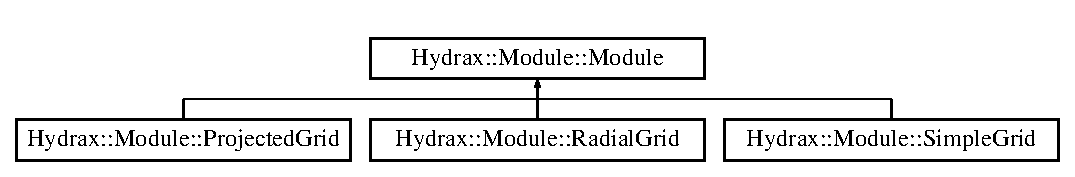
\includegraphics[height=1.93437cm]{class_hydrax_1_1_module_1_1_module}
\end{center}
\end{figure}
\subsection*{Public Member Functions}
\begin{CompactItemize}
\item 
\hyperlink{class_hydrax_1_1_module_1_1_module_b82e857eb19eac9c9091097909f3d566}{Module} (const Ogre::String \&Name, \hyperlink{class_hydrax_1_1_noise_1_1_noise}{Noise::Noise} $\ast$n, const \hyperlink{struct_hydrax_1_1_mesh_1_1_options}{Mesh::Options} \&MeshOptions, const \hyperlink{class_hydrax_1_1_material_manager_aa14689cd1c259f48954dfecda9b296f}{MaterialManager::NormalMode} \&NormalMode)
\item 
virtual \hyperlink{class_hydrax_1_1_module_1_1_module_0490f405b7150266765fb44ad1aefa8c}{$\sim$Module} ()
\item 
virtual void \hyperlink{class_hydrax_1_1_module_1_1_module_4b696328c3fc1496f757e929f44f3258}{create} ()
\item 
virtual void \hyperlink{class_hydrax_1_1_module_1_1_module_21f60a53a99d72ff00d3fe5565518165}{remove} ()
\item 
void \hyperlink{class_hydrax_1_1_module_1_1_module_f591ded25b7cbba848ec2853402fa91e}{setNoise} (\hyperlink{class_hydrax_1_1_noise_1_1_noise}{Noise::Noise} $\ast$Noise, \hyperlink{class_hydrax_1_1_g_p_u_normal_map_manager}{GPUNormalMapManager} $\ast$g=0, const bool \&DeleteOldNoise=true)
\item 
virtual void \hyperlink{class_hydrax_1_1_module_1_1_module_2042d450f99d9348fa4b7bd29ba89df3}{update} (const Ogre::Real \&timeSinceLastFrame)
\item 
virtual void \hyperlink{class_hydrax_1_1_module_1_1_module_998a5baf42f57b02ca7bc20bc12f95a9}{saveCfg} (Ogre::String \&Data)
\item 
virtual bool \hyperlink{class_hydrax_1_1_module_1_1_module_bedb96357608c0744bb7816ae1c2b0bb}{loadCfg} (Ogre::ConfigFile \&CfgFile)
\item 
const Ogre::String \& \hyperlink{class_hydrax_1_1_module_1_1_module_f00dbb4fcb83e45e89c7d537860ee486}{getName} () const 
\item 
const bool \& \hyperlink{class_hydrax_1_1_module_1_1_module_66097127eb529786f7384b4d39d9e43e}{isCreated} () const 
\item 
virtual const bool \hyperlink{class_hydrax_1_1_module_1_1_module_e58d6103f780287cb00a8c4647db667e}{\_\-createGeometry} (\hyperlink{class_hydrax_1_1_mesh}{Mesh} $\ast$mMesh) const 
\item 
const \hyperlink{class_hydrax_1_1_material_manager_aa14689cd1c259f48954dfecda9b296f}{MaterialManager::NormalMode} \& \hyperlink{class_hydrax_1_1_module_1_1_module_f5cfbabb783d9ded22f30f779c83c1c4}{getNormalMode} () const 
\item 
const \hyperlink{struct_hydrax_1_1_mesh_1_1_options}{Mesh::Options} \& \hyperlink{class_hydrax_1_1_module_1_1_module_7e083582d25431f9fbf83ce7eac77a94}{getMeshOptions} () const 
\item 
\hyperlink{class_hydrax_1_1_noise_1_1_noise}{Noise::Noise} $\ast$ \hyperlink{class_hydrax_1_1_module_1_1_module_e16db579f543cb24fdb7fcc909ee94cf}{getNoise} ()
\item 
virtual float \hyperlink{class_hydrax_1_1_module_1_1_module_c61f89589d3b1bc7256731ddb7af7d0b}{getHeigth} (const Ogre::Vector2 \&Position)
\end{CompactItemize}
\subsection*{Protected Attributes}
\begin{CompactItemize}
\item 
Ogre::String \hyperlink{class_hydrax_1_1_module_1_1_module_a478452f0e9c1bf8dde1526b30759de1}{mName}
\begin{CompactList}\small\item\em \hyperlink{class_hydrax_1_1_module_1_1_module}{Module} name. \item\end{CompactList}\item 
\hyperlink{class_hydrax_1_1_noise_1_1_noise}{Noise::Noise} $\ast$ \hyperlink{class_hydrax_1_1_module_1_1_module_9403c14c89393c8c7f562a1946ca05ab}{mNoise}
\begin{CompactList}\small\item\em \hyperlink{namespace_hydrax_1_1_noise}{Noise} generator pointer. \item\end{CompactList}\item 
\hyperlink{struct_hydrax_1_1_mesh_1_1_options}{Mesh::Options} \hyperlink{class_hydrax_1_1_module_1_1_module_99e803991d3d249baed293bdb40c56ed}{mMeshOptions}
\begin{CompactList}\small\item\em \hyperlink{class_hydrax_1_1_module_1_1_module}{Module} mesh options. \item\end{CompactList}\item 
\hyperlink{class_hydrax_1_1_material_manager_aa14689cd1c259f48954dfecda9b296f}{MaterialManager::NormalMode} \hyperlink{class_hydrax_1_1_module_1_1_module_962d19d1a608a3935440a08544919f13}{mNormalMode}
\begin{CompactList}\small\item\em Normal map generation mode. \item\end{CompactList}\item 
bool \hyperlink{class_hydrax_1_1_module_1_1_module_2b11bdd4cec12b483489e3987802a091}{mCreated}
\begin{CompactList}\small\item\em Is \hyperlink{class_hydrax_1_1_module_1_1_module_4b696328c3fc1496f757e929f44f3258}{create()} called? \item\end{CompactList}\end{CompactItemize}


\subsection{Detailed Description}
Base module class, Override it for create different ways of create water noise. 

\subsection{Constructor \& Destructor Documentation}
\hypertarget{class_hydrax_1_1_module_1_1_module_b82e857eb19eac9c9091097909f3d566}{
\index{Hydrax::Module::Module@{Hydrax::Module::Module}!Module@{Module}}
\index{Module@{Module}!Hydrax::Module::Module@{Hydrax::Module::Module}}
\subsubsection[{Module}]{\setlength{\rightskip}{0pt plus 5cm}Hydrax::Module::Module::Module (const Ogre::String \& {\em Name}, \/  {\bf Noise::Noise} $\ast$ {\em n}, \/  const {\bf Mesh::Options} \& {\em MeshOptions}, \/  const {\bf MaterialManager::NormalMode} \& {\em NormalMode})}}
\label{class_hydrax_1_1_module_1_1_module_b82e857eb19eac9c9091097909f3d566}


Constructor \begin{Desc}
\item[Parameters:]
\begin{description}
\item[{\em Name}]\hyperlink{class_hydrax_1_1_module_1_1_module}{Module} name \item[{\em n}]\hyperlink{class_hydrax_1_1_noise_1_1_noise}{Hydrax::Noise::Noise} generator pointer \item[{\em MeshOptions}]\hyperlink{class_hydrax_1_1_mesh}{Mesh} options \item[{\em NormalMode}]Normal generation mode \end{description}
\end{Desc}
\hypertarget{class_hydrax_1_1_module_1_1_module_0490f405b7150266765fb44ad1aefa8c}{
\index{Hydrax::Module::Module@{Hydrax::Module::Module}!$\sim$Module@{$\sim$Module}}
\index{$\sim$Module@{$\sim$Module}!Hydrax::Module::Module@{Hydrax::Module::Module}}
\subsubsection[{$\sim$Module}]{\setlength{\rightskip}{0pt plus 5cm}Hydrax::Module::Module::$\sim$Module ()\hspace{0.3cm}{\tt  \mbox{[}virtual\mbox{]}}}}
\label{class_hydrax_1_1_module_1_1_module_0490f405b7150266765fb44ad1aefa8c}


Destructor 

\subsection{Member Function Documentation}
\hypertarget{class_hydrax_1_1_module_1_1_module_e58d6103f780287cb00a8c4647db667e}{
\index{Hydrax::Module::Module@{Hydrax::Module::Module}!\_\-createGeometry@{\_\-createGeometry}}
\index{\_\-createGeometry@{\_\-createGeometry}!Hydrax::Module::Module@{Hydrax::Module::Module}}
\subsubsection[{\_\-createGeometry}]{\setlength{\rightskip}{0pt plus 5cm}virtual const bool Hydrax::Module::Module::\_\-createGeometry ({\bf Mesh} $\ast$ {\em mMesh}) const\hspace{0.3cm}{\tt  \mbox{[}inline, virtual\mbox{]}}}}
\label{class_hydrax_1_1_module_1_1_module_e58d6103f780287cb00a8c4647db667e}


Create geometry in module(If special geometry is needed) \begin{Desc}
\item[Parameters:]
\begin{description}
\item[{\em mMesh}]\hyperlink{class_hydrax_1_1_mesh}{Mesh} \end{description}
\end{Desc}
\begin{Desc}
\item[Returns:]false if it must be create by default Mesh::\_\-createGeometry() fnc. \end{Desc}
\begin{Desc}
\item[Remarks:]Override it if any especial geometry mesh creation is needed. \end{Desc}


Reimplemented in \hyperlink{class_hydrax_1_1_module_1_1_radial_grid_8fde866e72e871e7aaf76957236b7b15}{Hydrax::Module::RadialGrid}.\hypertarget{class_hydrax_1_1_module_1_1_module_4b696328c3fc1496f757e929f44f3258}{
\index{Hydrax::Module::Module@{Hydrax::Module::Module}!create@{create}}
\index{create@{create}!Hydrax::Module::Module@{Hydrax::Module::Module}}
\subsubsection[{create}]{\setlength{\rightskip}{0pt plus 5cm}void Hydrax::Module::Module::create ()\hspace{0.3cm}{\tt  \mbox{[}virtual\mbox{]}}}}
\label{class_hydrax_1_1_module_1_1_module_4b696328c3fc1496f757e929f44f3258}


Create \begin{Desc}
\item[Remarks:]Not forgot call in the override class \end{Desc}


Reimplemented in \hyperlink{class_hydrax_1_1_module_1_1_projected_grid_86e4648a741558934e664f7400082742}{Hydrax::Module::ProjectedGrid}, \hyperlink{class_hydrax_1_1_module_1_1_radial_grid_8c0f059e53170e7d1114bb7faecbcb0a}{Hydrax::Module::RadialGrid}, and \hyperlink{class_hydrax_1_1_module_1_1_simple_grid_7e52fb7497f6a2d27666a384d7a1d003}{Hydrax::Module::SimpleGrid}.\hypertarget{class_hydrax_1_1_module_1_1_module_c61f89589d3b1bc7256731ddb7af7d0b}{
\index{Hydrax::Module::Module@{Hydrax::Module::Module}!getHeigth@{getHeigth}}
\index{getHeigth@{getHeigth}!Hydrax::Module::Module@{Hydrax::Module::Module}}
\subsubsection[{getHeigth}]{\setlength{\rightskip}{0pt plus 5cm}float Hydrax::Module::Module::getHeigth (const Ogre::Vector2 \& {\em Position})\hspace{0.3cm}{\tt  \mbox{[}virtual\mbox{]}}}}
\label{class_hydrax_1_1_module_1_1_module_c61f89589d3b1bc7256731ddb7af7d0b}


Get the current heigth at a especified world-space point \begin{Desc}
\item[Parameters:]
\begin{description}
\item[{\em Position}]X/Z World position \end{description}
\end{Desc}
\begin{Desc}
\item[Returns:]Heigth at the given position in y-World coordinates, if it's outside of the water return -1 \end{Desc}


Reimplemented in \hyperlink{class_hydrax_1_1_module_1_1_projected_grid_a7a5b8100642a55f23b4d1c0a125bd62}{Hydrax::Module::ProjectedGrid}, \hyperlink{class_hydrax_1_1_module_1_1_radial_grid_0289caac51efbaf6a085bbb94eb22c4c}{Hydrax::Module::RadialGrid}, and \hyperlink{class_hydrax_1_1_module_1_1_simple_grid_9a9e5bba632f0317c82370fa433559ac}{Hydrax::Module::SimpleGrid}.\hypertarget{class_hydrax_1_1_module_1_1_module_7e083582d25431f9fbf83ce7eac77a94}{
\index{Hydrax::Module::Module@{Hydrax::Module::Module}!getMeshOptions@{getMeshOptions}}
\index{getMeshOptions@{getMeshOptions}!Hydrax::Module::Module@{Hydrax::Module::Module}}
\subsubsection[{getMeshOptions}]{\setlength{\rightskip}{0pt plus 5cm}const {\bf Mesh::Options}\& Hydrax::Module::Module::getMeshOptions () const\hspace{0.3cm}{\tt  \mbox{[}inline\mbox{]}}}}
\label{class_hydrax_1_1_module_1_1_module_7e083582d25431f9fbf83ce7eac77a94}


Get the mesh options for this module \begin{Desc}
\item[Returns:]\hyperlink{class_hydrax_1_1_mesh}{Mesh} options for this module \end{Desc}
\hypertarget{class_hydrax_1_1_module_1_1_module_f00dbb4fcb83e45e89c7d537860ee486}{
\index{Hydrax::Module::Module@{Hydrax::Module::Module}!getName@{getName}}
\index{getName@{getName}!Hydrax::Module::Module@{Hydrax::Module::Module}}
\subsubsection[{getName}]{\setlength{\rightskip}{0pt plus 5cm}const Ogre::String\& Hydrax::Module::Module::getName () const\hspace{0.3cm}{\tt  \mbox{[}inline\mbox{]}}}}
\label{class_hydrax_1_1_module_1_1_module_f00dbb4fcb83e45e89c7d537860ee486}


Get module name \begin{Desc}
\item[Returns:]\hyperlink{class_hydrax_1_1_module_1_1_module}{Module} name \end{Desc}
\hypertarget{class_hydrax_1_1_module_1_1_module_e16db579f543cb24fdb7fcc909ee94cf}{
\index{Hydrax::Module::Module@{Hydrax::Module::Module}!getNoise@{getNoise}}
\index{getNoise@{getNoise}!Hydrax::Module::Module@{Hydrax::Module::Module}}
\subsubsection[{getNoise}]{\setlength{\rightskip}{0pt plus 5cm}{\bf Noise::Noise}$\ast$ Hydrax::Module::Module::getNoise ()\hspace{0.3cm}{\tt  \mbox{[}inline\mbox{]}}}}
\label{class_hydrax_1_1_module_1_1_module_e16db579f543cb24fdb7fcc909ee94cf}


Get the \hyperlink{namespace_hydrax_1_1_noise}{Hydrax::Noise} module pointer \begin{Desc}
\item[Returns:]\hyperlink{namespace_hydrax_1_1_noise}{Hydrax::Noise} pointer \end{Desc}
\hypertarget{class_hydrax_1_1_module_1_1_module_f5cfbabb783d9ded22f30f779c83c1c4}{
\index{Hydrax::Module::Module@{Hydrax::Module::Module}!getNormalMode@{getNormalMode}}
\index{getNormalMode@{getNormalMode}!Hydrax::Module::Module@{Hydrax::Module::Module}}
\subsubsection[{getNormalMode}]{\setlength{\rightskip}{0pt plus 5cm}const {\bf MaterialManager::NormalMode}\& Hydrax::Module::Module::getNormalMode () const\hspace{0.3cm}{\tt  \mbox{[}inline\mbox{]}}}}
\label{class_hydrax_1_1_module_1_1_module_f5cfbabb783d9ded22f30f779c83c1c4}


Get the normal generation mode \begin{Desc}
\item[Returns:]\hyperlink{class_hydrax_1_1_module_1_1_module}{Module} normal generation mode \end{Desc}
\hypertarget{class_hydrax_1_1_module_1_1_module_66097127eb529786f7384b4d39d9e43e}{
\index{Hydrax::Module::Module@{Hydrax::Module::Module}!isCreated@{isCreated}}
\index{isCreated@{isCreated}!Hydrax::Module::Module@{Hydrax::Module::Module}}
\subsubsection[{isCreated}]{\setlength{\rightskip}{0pt plus 5cm}const bool\& Hydrax::Module::Module::isCreated () const\hspace{0.3cm}{\tt  \mbox{[}inline\mbox{]}}}}
\label{class_hydrax_1_1_module_1_1_module_66097127eb529786f7384b4d39d9e43e}


Is created() called? \begin{Desc}
\item[Returns:]true if created() have been already called \end{Desc}
\hypertarget{class_hydrax_1_1_module_1_1_module_bedb96357608c0744bb7816ae1c2b0bb}{
\index{Hydrax::Module::Module@{Hydrax::Module::Module}!loadCfg@{loadCfg}}
\index{loadCfg@{loadCfg}!Hydrax::Module::Module@{Hydrax::Module::Module}}
\subsubsection[{loadCfg}]{\setlength{\rightskip}{0pt plus 5cm}bool Hydrax::Module::Module::loadCfg (Ogre::ConfigFile \& {\em CfgFile})\hspace{0.3cm}{\tt  \mbox{[}virtual\mbox{]}}}}
\label{class_hydrax_1_1_module_1_1_module_bedb96357608c0744bb7816ae1c2b0bb}


Load config \begin{Desc}
\item[Parameters:]
\begin{description}
\item[{\em CgfFile}]Ogre::ConfigFile reference \end{description}
\end{Desc}
\begin{Desc}
\item[Returns:]True if is the correct module config \end{Desc}


Reimplemented in \hyperlink{class_hydrax_1_1_module_1_1_projected_grid_f951c58cc93cf75d57e69aa14a668d3e}{Hydrax::Module::ProjectedGrid}, \hyperlink{class_hydrax_1_1_module_1_1_radial_grid_31b3bab8e74f2f1e316a1800470ac685}{Hydrax::Module::RadialGrid}, and \hyperlink{class_hydrax_1_1_module_1_1_simple_grid_3741ec1a3df1863e730711fd9d3b14e1}{Hydrax::Module::SimpleGrid}.\hypertarget{class_hydrax_1_1_module_1_1_module_21f60a53a99d72ff00d3fe5565518165}{
\index{Hydrax::Module::Module@{Hydrax::Module::Module}!remove@{remove}}
\index{remove@{remove}!Hydrax::Module::Module@{Hydrax::Module::Module}}
\subsubsection[{remove}]{\setlength{\rightskip}{0pt plus 5cm}void Hydrax::Module::Module::remove ()\hspace{0.3cm}{\tt  \mbox{[}virtual\mbox{]}}}}
\label{class_hydrax_1_1_module_1_1_module_21f60a53a99d72ff00d3fe5565518165}


Remove \begin{Desc}
\item[Remarks:]Not forgot call in the override class \end{Desc}


Reimplemented in \hyperlink{class_hydrax_1_1_module_1_1_projected_grid_b878b7d1258aacda8bee0f2e945ea64d}{Hydrax::Module::ProjectedGrid}, \hyperlink{class_hydrax_1_1_module_1_1_radial_grid_5b595aede4b235740be75fb5cf1072cf}{Hydrax::Module::RadialGrid}, and \hyperlink{class_hydrax_1_1_module_1_1_simple_grid_ca3e257313599b797b8a65442cecd3cc}{Hydrax::Module::SimpleGrid}.\hypertarget{class_hydrax_1_1_module_1_1_module_998a5baf42f57b02ca7bc20bc12f95a9}{
\index{Hydrax::Module::Module@{Hydrax::Module::Module}!saveCfg@{saveCfg}}
\index{saveCfg@{saveCfg}!Hydrax::Module::Module@{Hydrax::Module::Module}}
\subsubsection[{saveCfg}]{\setlength{\rightskip}{0pt plus 5cm}void Hydrax::Module::Module::saveCfg (Ogre::String \& {\em Data})\hspace{0.3cm}{\tt  \mbox{[}virtual\mbox{]}}}}
\label{class_hydrax_1_1_module_1_1_module_998a5baf42f57b02ca7bc20bc12f95a9}


Save config \begin{Desc}
\item[Parameters:]
\begin{description}
\item[{\em Data}]String reference \end{description}
\end{Desc}


Reimplemented in \hyperlink{class_hydrax_1_1_module_1_1_projected_grid_4502387739439e0d6cca1f006fc4a28c}{Hydrax::Module::ProjectedGrid}, \hyperlink{class_hydrax_1_1_module_1_1_radial_grid_241237552e8f36f7e4696b8bad7acc91}{Hydrax::Module::RadialGrid}, and \hyperlink{class_hydrax_1_1_module_1_1_simple_grid_f79cb3a457da1fe8b015d9d7b5a6a376}{Hydrax::Module::SimpleGrid}.\hypertarget{class_hydrax_1_1_module_1_1_module_f591ded25b7cbba848ec2853402fa91e}{
\index{Hydrax::Module::Module@{Hydrax::Module::Module}!setNoise@{setNoise}}
\index{setNoise@{setNoise}!Hydrax::Module::Module@{Hydrax::Module::Module}}
\subsubsection[{setNoise}]{\setlength{\rightskip}{0pt plus 5cm}void Hydrax::Module::Module::setNoise ({\bf Noise::Noise} $\ast$ {\em Noise}, \/  {\bf GPUNormalMapManager} $\ast$ {\em g} = {\tt 0}, \/  const bool \& {\em DeleteOldNoise} = {\tt true})}}
\label{class_hydrax_1_1_module_1_1_module_f591ded25b7cbba848ec2853402fa91e}


Set noise \begin{Desc}
\item[Parameters:]
\begin{description}
\item[{\em \hyperlink{namespace_hydrax_1_1_noise}{Noise}}]New noise module \item[{\em g}]\hyperlink{class_hydrax_1_1_g_p_u_normal_map_manager}{GPUNormalMapManager} pointer, default: NULL, use it if GPU Normal map generation is needed \item[{\em DeleteOldNoise}]Delete the old noise module (Default = true) \end{description}
\end{Desc}
\hypertarget{class_hydrax_1_1_module_1_1_module_2042d450f99d9348fa4b7bd29ba89df3}{
\index{Hydrax::Module::Module@{Hydrax::Module::Module}!update@{update}}
\index{update@{update}!Hydrax::Module::Module@{Hydrax::Module::Module}}
\subsubsection[{update}]{\setlength{\rightskip}{0pt plus 5cm}void Hydrax::Module::Module::update (const Ogre::Real \& {\em timeSinceLastFrame})\hspace{0.3cm}{\tt  \mbox{[}virtual\mbox{]}}}}
\label{class_hydrax_1_1_module_1_1_module_2042d450f99d9348fa4b7bd29ba89df3}


Call it each frame \begin{Desc}
\item[Parameters:]
\begin{description}
\item[{\em timeSinceLastFrame}]Time since last frame(delta) \end{description}
\end{Desc}


Reimplemented in \hyperlink{class_hydrax_1_1_module_1_1_projected_grid_8d7a8efcd6b7fd0e4313c9114bd2c061}{Hydrax::Module::ProjectedGrid}, \hyperlink{class_hydrax_1_1_module_1_1_radial_grid_ee5199bfbee4429ab428d477e36443dd}{Hydrax::Module::RadialGrid}, and \hyperlink{class_hydrax_1_1_module_1_1_simple_grid_aa120d4f487785136a3134cc8980fb16}{Hydrax::Module::SimpleGrid}.

\subsection{Member Data Documentation}
\hypertarget{class_hydrax_1_1_module_1_1_module_2b11bdd4cec12b483489e3987802a091}{
\index{Hydrax::Module::Module@{Hydrax::Module::Module}!mCreated@{mCreated}}
\index{mCreated@{mCreated}!Hydrax::Module::Module@{Hydrax::Module::Module}}
\subsubsection[{mCreated}]{\setlength{\rightskip}{0pt plus 5cm}bool {\bf Hydrax::Module::Module::mCreated}\hspace{0.3cm}{\tt  \mbox{[}protected\mbox{]}}}}
\label{class_hydrax_1_1_module_1_1_module_2b11bdd4cec12b483489e3987802a091}


Is \hyperlink{class_hydrax_1_1_module_1_1_module_4b696328c3fc1496f757e929f44f3258}{create()} called? 

\hypertarget{class_hydrax_1_1_module_1_1_module_99e803991d3d249baed293bdb40c56ed}{
\index{Hydrax::Module::Module@{Hydrax::Module::Module}!mMeshOptions@{mMeshOptions}}
\index{mMeshOptions@{mMeshOptions}!Hydrax::Module::Module@{Hydrax::Module::Module}}
\subsubsection[{mMeshOptions}]{\setlength{\rightskip}{0pt plus 5cm}{\bf Mesh::Options} {\bf Hydrax::Module::Module::mMeshOptions}\hspace{0.3cm}{\tt  \mbox{[}protected\mbox{]}}}}
\label{class_hydrax_1_1_module_1_1_module_99e803991d3d249baed293bdb40c56ed}


\hyperlink{class_hydrax_1_1_module_1_1_module}{Module} mesh options. 

\hypertarget{class_hydrax_1_1_module_1_1_module_a478452f0e9c1bf8dde1526b30759de1}{
\index{Hydrax::Module::Module@{Hydrax::Module::Module}!mName@{mName}}
\index{mName@{mName}!Hydrax::Module::Module@{Hydrax::Module::Module}}
\subsubsection[{mName}]{\setlength{\rightskip}{0pt plus 5cm}Ogre::String {\bf Hydrax::Module::Module::mName}\hspace{0.3cm}{\tt  \mbox{[}protected\mbox{]}}}}
\label{class_hydrax_1_1_module_1_1_module_a478452f0e9c1bf8dde1526b30759de1}


\hyperlink{class_hydrax_1_1_module_1_1_module}{Module} name. 

\hypertarget{class_hydrax_1_1_module_1_1_module_9403c14c89393c8c7f562a1946ca05ab}{
\index{Hydrax::Module::Module@{Hydrax::Module::Module}!mNoise@{mNoise}}
\index{mNoise@{mNoise}!Hydrax::Module::Module@{Hydrax::Module::Module}}
\subsubsection[{mNoise}]{\setlength{\rightskip}{0pt plus 5cm}{\bf Noise::Noise}$\ast$ {\bf Hydrax::Module::Module::mNoise}\hspace{0.3cm}{\tt  \mbox{[}protected\mbox{]}}}}
\label{class_hydrax_1_1_module_1_1_module_9403c14c89393c8c7f562a1946ca05ab}


\hyperlink{namespace_hydrax_1_1_noise}{Noise} generator pointer. 

\hypertarget{class_hydrax_1_1_module_1_1_module_962d19d1a608a3935440a08544919f13}{
\index{Hydrax::Module::Module@{Hydrax::Module::Module}!mNormalMode@{mNormalMode}}
\index{mNormalMode@{mNormalMode}!Hydrax::Module::Module@{Hydrax::Module::Module}}
\subsubsection[{mNormalMode}]{\setlength{\rightskip}{0pt plus 5cm}{\bf MaterialManager::NormalMode} {\bf Hydrax::Module::Module::mNormalMode}\hspace{0.3cm}{\tt  \mbox{[}protected\mbox{]}}}}
\label{class_hydrax_1_1_module_1_1_module_962d19d1a608a3935440a08544919f13}


Normal map generation mode. 



The documentation for this class was generated from the following files:\begin{CompactItemize}
\item 
C:/Hydrax/v0.5.1/Hydrax/src/Hydrax/Modules/\hyperlink{_module_8h}{Module.h}\item 
C:/Hydrax/v0.5.1/Hydrax/src/Hydrax/Modules/\hyperlink{_module_8cpp}{Module.cpp}\end{CompactItemize}

\hypertarget{class_hydrax_1_1_noise_1_1_noise}{
\section{Hydrax::Noise::Noise Class Reference}
\label{class_hydrax_1_1_noise_1_1_noise}\index{Hydrax::Noise::Noise@{Hydrax::Noise::Noise}}
}
{\tt \#include $<$Noise.h$>$}

Inheritance diagram for Hydrax::Noise::Noise::\begin{figure}[H]
\begin{center}
\leavevmode
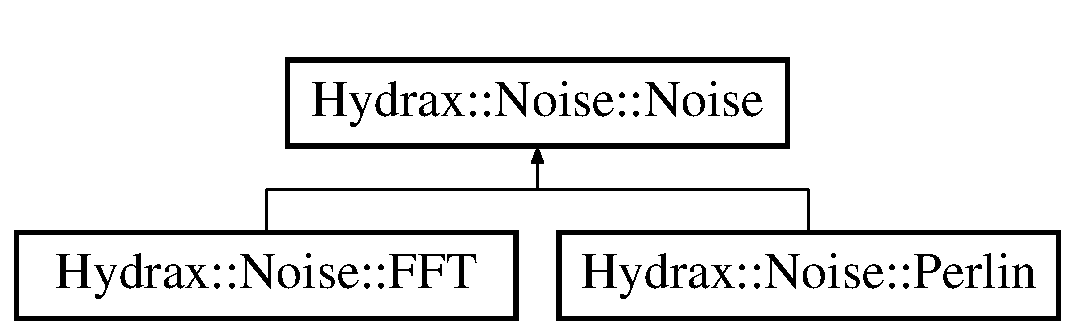
\includegraphics[height=2cm]{class_hydrax_1_1_noise_1_1_noise}
\end{center}
\end{figure}
\subsection*{Public Member Functions}
\begin{CompactItemize}
\item 
\hyperlink{class_hydrax_1_1_noise_1_1_noise_18d24fbe43250f986c5d5c57e1780f19}{Noise} (const Ogre::String \&Name, const bool \&GPUNormalMapSupported)
\item 
virtual \hyperlink{class_hydrax_1_1_noise_1_1_noise_4ff5ce1a68da081f11015cdc4b417f15}{$\sim$Noise} ()
\item 
virtual void \hyperlink{class_hydrax_1_1_noise_1_1_noise_be9cf8765feed765e6a35b0779125f6a}{create} ()
\item 
virtual void \hyperlink{class_hydrax_1_1_noise_1_1_noise_00c4aaa7604ea492740318d01f651606}{remove} ()
\item 
virtual bool \hyperlink{class_hydrax_1_1_noise_1_1_noise_59f0e03e88a5de69065838adc35ff2d8}{createGPUNormalMapResources} (\hyperlink{class_hydrax_1_1_g_p_u_normal_map_manager}{GPUNormalMapManager} $\ast$g)
\item 
virtual void \hyperlink{class_hydrax_1_1_noise_1_1_noise_9d3ca345d3f5b629e43ab276236d93b7}{removeGPUNormalMapResources} (\hyperlink{class_hydrax_1_1_g_p_u_normal_map_manager}{GPUNormalMapManager} $\ast$g)
\item 
virtual void \hyperlink{class_hydrax_1_1_noise_1_1_noise_9c32c4c630f193e034c074f69ea10f57}{update} (const Ogre::Real \&timeSinceLastFrame)=0
\item 
virtual void \hyperlink{class_hydrax_1_1_noise_1_1_noise_ac0a9fe1533ddd87467edb954f8abea8}{saveCfg} (Ogre::String \&Data)
\item 
virtual bool \hyperlink{class_hydrax_1_1_noise_1_1_noise_5ef6e71282a9dfcefc09e3ba84a7578f}{loadCfg} (Ogre::ConfigFile \&CfgFile)
\item 
const Ogre::String \& \hyperlink{class_hydrax_1_1_noise_1_1_noise_bd7bddafc148656d1a7782c94fb4a7aa}{getName} () const 
\item 
const bool \& \hyperlink{class_hydrax_1_1_noise_1_1_noise_94f5963b8f6fed2fb22149ff22e1166f}{isCreated} () const 
\item 
const bool \& \hyperlink{class_hydrax_1_1_noise_1_1_noise_20e13eb2f5cc93d384bb846b05d7aaeb}{isGPUNormalMapSupported} () const 
\item 
const bool \& \hyperlink{class_hydrax_1_1_noise_1_1_noise_e2260556005e5a5eaebae94d936b60c0}{areGPUNormalMapResourcesCreated} () const 
\item 
virtual float \hyperlink{class_hydrax_1_1_noise_1_1_noise_5b18138d5c2c5ea3c3659cef80dd3a3e}{getValue} (const float \&x, const float \&y)=0
\end{CompactItemize}
\subsection*{Protected Attributes}
\begin{CompactItemize}
\item 
Ogre::String \hyperlink{class_hydrax_1_1_noise_1_1_noise_aedee8210b700f1ee80c660a38973b14}{mName}
\begin{CompactList}\small\item\em \hyperlink{namespace_hydrax_1_1_module}{Module} name. \item\end{CompactList}\item 
bool \hyperlink{class_hydrax_1_1_noise_1_1_noise_7a0bdaab63fa4a2feec69afe5be5ab19}{mCreated}
\begin{CompactList}\small\item\em Has \hyperlink{class_hydrax_1_1_noise_1_1_noise_be9cf8765feed765e6a35b0779125f6a}{create()} been already called? \item\end{CompactList}\item 
bool \hyperlink{class_hydrax_1_1_noise_1_1_noise_ce28ba855518ef99599c1ac4a7512446}{mGPUNormalMapSupported}
\begin{CompactList}\small\item\em Is GPU normal map generation supported? \item\end{CompactList}\item 
bool \hyperlink{class_hydrax_1_1_noise_1_1_noise_8c140b20c56920d4dd99204dff093ac2}{mGPUNormalMapResourcesCreated}
\begin{CompactList}\small\item\em Are GPU normal map resources created? \item\end{CompactList}\end{CompactItemize}


\subsection{Detailed Description}
Base noise class, Override it for create different ways of create water noise. 

\subsection{Constructor \& Destructor Documentation}
\hypertarget{class_hydrax_1_1_noise_1_1_noise_18d24fbe43250f986c5d5c57e1780f19}{
\index{Hydrax::Noise::Noise@{Hydrax::Noise::Noise}!Noise@{Noise}}
\index{Noise@{Noise}!Hydrax::Noise::Noise@{Hydrax::Noise::Noise}}
\subsubsection[{Noise}]{\setlength{\rightskip}{0pt plus 5cm}Hydrax::Noise::Noise::Noise (const Ogre::String \& {\em Name}, \/  const bool \& {\em GPUNormalMapSupported})}}
\label{class_hydrax_1_1_noise_1_1_noise_18d24fbe43250f986c5d5c57e1780f19}


Constructor \begin{Desc}
\item[Parameters:]
\begin{description}
\item[{\em Name}]\hyperlink{class_hydrax_1_1_noise_1_1_noise}{Noise} name \item[{\em GPUNormalMapSupported}]Is GPU normal map generation supported? \end{description}
\end{Desc}
\hypertarget{class_hydrax_1_1_noise_1_1_noise_4ff5ce1a68da081f11015cdc4b417f15}{
\index{Hydrax::Noise::Noise@{Hydrax::Noise::Noise}!$\sim$Noise@{$\sim$Noise}}
\index{$\sim$Noise@{$\sim$Noise}!Hydrax::Noise::Noise@{Hydrax::Noise::Noise}}
\subsubsection[{$\sim$Noise}]{\setlength{\rightskip}{0pt plus 5cm}Hydrax::Noise::Noise::$\sim$Noise ()\hspace{0.3cm}{\tt  \mbox{[}virtual\mbox{]}}}}
\label{class_hydrax_1_1_noise_1_1_noise_4ff5ce1a68da081f11015cdc4b417f15}


Destructor 

\subsection{Member Function Documentation}
\hypertarget{class_hydrax_1_1_noise_1_1_noise_e2260556005e5a5eaebae94d936b60c0}{
\index{Hydrax::Noise::Noise@{Hydrax::Noise::Noise}!areGPUNormalMapResourcesCreated@{areGPUNormalMapResourcesCreated}}
\index{areGPUNormalMapResourcesCreated@{areGPUNormalMapResourcesCreated}!Hydrax::Noise::Noise@{Hydrax::Noise::Noise}}
\subsubsection[{areGPUNormalMapResourcesCreated}]{\setlength{\rightskip}{0pt plus 5cm}const bool\& Hydrax::Noise::Noise::areGPUNormalMapResourcesCreated () const\hspace{0.3cm}{\tt  \mbox{[}inline\mbox{]}}}}
\label{class_hydrax_1_1_noise_1_1_noise_e2260556005e5a5eaebae94d936b60c0}


Are GPU normal map resources created? \begin{Desc}
\item[Returns:]true if yes, false if not \end{Desc}
\hypertarget{class_hydrax_1_1_noise_1_1_noise_be9cf8765feed765e6a35b0779125f6a}{
\index{Hydrax::Noise::Noise@{Hydrax::Noise::Noise}!create@{create}}
\index{create@{create}!Hydrax::Noise::Noise@{Hydrax::Noise::Noise}}
\subsubsection[{create}]{\setlength{\rightskip}{0pt plus 5cm}void Hydrax::Noise::Noise::create ()\hspace{0.3cm}{\tt  \mbox{[}virtual\mbox{]}}}}
\label{class_hydrax_1_1_noise_1_1_noise_be9cf8765feed765e6a35b0779125f6a}


Create 

Reimplemented in \hyperlink{class_hydrax_1_1_noise_1_1_f_f_t_c382e8624b864a32267687592b769bd3}{Hydrax::Noise::FFT}, and \hyperlink{class_hydrax_1_1_noise_1_1_perlin_3e260e7c239d90da210aa3e27289c6f0}{Hydrax::Noise::Perlin}.\hypertarget{class_hydrax_1_1_noise_1_1_noise_59f0e03e88a5de69065838adc35ff2d8}{
\index{Hydrax::Noise::Noise@{Hydrax::Noise::Noise}!createGPUNormalMapResources@{createGPUNormalMapResources}}
\index{createGPUNormalMapResources@{createGPUNormalMapResources}!Hydrax::Noise::Noise@{Hydrax::Noise::Noise}}
\subsubsection[{createGPUNormalMapResources}]{\setlength{\rightskip}{0pt plus 5cm}bool Hydrax::Noise::Noise::createGPUNormalMapResources ({\bf GPUNormalMapManager} $\ast$ {\em g})\hspace{0.3cm}{\tt  \mbox{[}virtual\mbox{]}}}}
\label{class_hydrax_1_1_noise_1_1_noise_59f0e03e88a5de69065838adc35ff2d8}


Create GPUNormalMap resources \begin{Desc}
\item[Parameters:]
\begin{description}
\item[{\em g}]\hyperlink{class_hydrax_1_1_g_p_u_normal_map_manager}{GPUNormalMapManager} pointer \end{description}
\end{Desc}
\begin{Desc}
\item[Returns:]true if it needs to be created, false if not \end{Desc}


Reimplemented in \hyperlink{class_hydrax_1_1_noise_1_1_f_f_t_a8e2b9d2b8307c07be2d2cd9cf115560}{Hydrax::Noise::FFT}, and \hyperlink{class_hydrax_1_1_noise_1_1_perlin_db347b98692bd7ce6ad7ce76c605d15a}{Hydrax::Noise::Perlin}.\hypertarget{class_hydrax_1_1_noise_1_1_noise_bd7bddafc148656d1a7782c94fb4a7aa}{
\index{Hydrax::Noise::Noise@{Hydrax::Noise::Noise}!getName@{getName}}
\index{getName@{getName}!Hydrax::Noise::Noise@{Hydrax::Noise::Noise}}
\subsubsection[{getName}]{\setlength{\rightskip}{0pt plus 5cm}const Ogre::String\& Hydrax::Noise::Noise::getName () const\hspace{0.3cm}{\tt  \mbox{[}inline\mbox{]}}}}
\label{class_hydrax_1_1_noise_1_1_noise_bd7bddafc148656d1a7782c94fb4a7aa}


Get noise name \begin{Desc}
\item[Returns:]\hyperlink{class_hydrax_1_1_noise_1_1_noise}{Noise} name \end{Desc}
\hypertarget{class_hydrax_1_1_noise_1_1_noise_5b18138d5c2c5ea3c3659cef80dd3a3e}{
\index{Hydrax::Noise::Noise@{Hydrax::Noise::Noise}!getValue@{getValue}}
\index{getValue@{getValue}!Hydrax::Noise::Noise@{Hydrax::Noise::Noise}}
\subsubsection[{getValue}]{\setlength{\rightskip}{0pt plus 5cm}virtual float Hydrax::Noise::Noise::getValue (const float \& {\em x}, \/  const float \& {\em y})\hspace{0.3cm}{\tt  \mbox{[}pure virtual\mbox{]}}}}
\label{class_hydrax_1_1_noise_1_1_noise_5b18138d5c2c5ea3c3659cef80dd3a3e}


Get the especified x/y noise value \begin{Desc}
\item[Parameters:]
\begin{description}
\item[{\em x}]X Coord \item[{\em y}]Y Coord \end{description}
\end{Desc}
\begin{Desc}
\item[Returns:]\hyperlink{class_hydrax_1_1_noise_1_1_noise}{Noise} value \end{Desc}


Implemented in \hyperlink{class_hydrax_1_1_noise_1_1_f_f_t_e7da5bf6c6ebfc9061ed433af6350ea7}{Hydrax::Noise::FFT}, and \hyperlink{class_hydrax_1_1_noise_1_1_perlin_64bbe19643e0a87c08c62d0e73d7aac6}{Hydrax::Noise::Perlin}.\hypertarget{class_hydrax_1_1_noise_1_1_noise_94f5963b8f6fed2fb22149ff22e1166f}{
\index{Hydrax::Noise::Noise@{Hydrax::Noise::Noise}!isCreated@{isCreated}}
\index{isCreated@{isCreated}!Hydrax::Noise::Noise@{Hydrax::Noise::Noise}}
\subsubsection[{isCreated}]{\setlength{\rightskip}{0pt plus 5cm}const bool\& Hydrax::Noise::Noise::isCreated () const\hspace{0.3cm}{\tt  \mbox{[}inline\mbox{]}}}}
\label{class_hydrax_1_1_noise_1_1_noise_94f5963b8f6fed2fb22149ff22e1166f}


Is created() called? \begin{Desc}
\item[Returns:]true if \hyperlink{class_hydrax_1_1_noise_1_1_noise_be9cf8765feed765e6a35b0779125f6a}{create()} have been already called \end{Desc}
\hypertarget{class_hydrax_1_1_noise_1_1_noise_20e13eb2f5cc93d384bb846b05d7aaeb}{
\index{Hydrax::Noise::Noise@{Hydrax::Noise::Noise}!isGPUNormalMapSupported@{isGPUNormalMapSupported}}
\index{isGPUNormalMapSupported@{isGPUNormalMapSupported}!Hydrax::Noise::Noise@{Hydrax::Noise::Noise}}
\subsubsection[{isGPUNormalMapSupported}]{\setlength{\rightskip}{0pt plus 5cm}const bool\& Hydrax::Noise::Noise::isGPUNormalMapSupported () const\hspace{0.3cm}{\tt  \mbox{[}inline\mbox{]}}}}
\label{class_hydrax_1_1_noise_1_1_noise_20e13eb2f5cc93d384bb846b05d7aaeb}


Is GPU Normal map generation supported \begin{Desc}
\item[Returns:]true if yes, false if not \end{Desc}
\hypertarget{class_hydrax_1_1_noise_1_1_noise_5ef6e71282a9dfcefc09e3ba84a7578f}{
\index{Hydrax::Noise::Noise@{Hydrax::Noise::Noise}!loadCfg@{loadCfg}}
\index{loadCfg@{loadCfg}!Hydrax::Noise::Noise@{Hydrax::Noise::Noise}}
\subsubsection[{loadCfg}]{\setlength{\rightskip}{0pt plus 5cm}bool Hydrax::Noise::Noise::loadCfg (Ogre::ConfigFile \& {\em CfgFile})\hspace{0.3cm}{\tt  \mbox{[}virtual\mbox{]}}}}
\label{class_hydrax_1_1_noise_1_1_noise_5ef6e71282a9dfcefc09e3ba84a7578f}


Load config \begin{Desc}
\item[Parameters:]
\begin{description}
\item[{\em CgfFile}]Ogre::ConfigFile reference \end{description}
\end{Desc}
\begin{Desc}
\item[Returns:]True if is the correct noise config \end{Desc}


Reimplemented in \hyperlink{class_hydrax_1_1_noise_1_1_f_f_t_64245b9e56eeb8627ac3f5260dc203dd}{Hydrax::Noise::FFT}, and \hyperlink{class_hydrax_1_1_noise_1_1_perlin_3a2dab14cfbda1ccf8fc5de4bb89f124}{Hydrax::Noise::Perlin}.\hypertarget{class_hydrax_1_1_noise_1_1_noise_00c4aaa7604ea492740318d01f651606}{
\index{Hydrax::Noise::Noise@{Hydrax::Noise::Noise}!remove@{remove}}
\index{remove@{remove}!Hydrax::Noise::Noise@{Hydrax::Noise::Noise}}
\subsubsection[{remove}]{\setlength{\rightskip}{0pt plus 5cm}void Hydrax::Noise::Noise::remove ()\hspace{0.3cm}{\tt  \mbox{[}virtual\mbox{]}}}}
\label{class_hydrax_1_1_noise_1_1_noise_00c4aaa7604ea492740318d01f651606}


Remove 

Reimplemented in \hyperlink{class_hydrax_1_1_noise_1_1_f_f_t_9567d90d8fae8dbd74d05d1e3b8281e4}{Hydrax::Noise::FFT}, and \hyperlink{class_hydrax_1_1_noise_1_1_perlin_666010a5142bbb2b03c97aa5aa7bdef1}{Hydrax::Noise::Perlin}.\hypertarget{class_hydrax_1_1_noise_1_1_noise_9d3ca345d3f5b629e43ab276236d93b7}{
\index{Hydrax::Noise::Noise@{Hydrax::Noise::Noise}!removeGPUNormalMapResources@{removeGPUNormalMapResources}}
\index{removeGPUNormalMapResources@{removeGPUNormalMapResources}!Hydrax::Noise::Noise@{Hydrax::Noise::Noise}}
\subsubsection[{removeGPUNormalMapResources}]{\setlength{\rightskip}{0pt plus 5cm}void Hydrax::Noise::Noise::removeGPUNormalMapResources ({\bf GPUNormalMapManager} $\ast$ {\em g})\hspace{0.3cm}{\tt  \mbox{[}virtual\mbox{]}}}}
\label{class_hydrax_1_1_noise_1_1_noise_9d3ca345d3f5b629e43ab276236d93b7}


Remove GPUNormalMap resources \begin{Desc}
\item[Parameters:]
\begin{description}
\item[{\em g}]\hyperlink{class_hydrax_1_1_g_p_u_normal_map_manager}{GPUNormalMapManager} pointer \end{description}
\end{Desc}
\hypertarget{class_hydrax_1_1_noise_1_1_noise_ac0a9fe1533ddd87467edb954f8abea8}{
\index{Hydrax::Noise::Noise@{Hydrax::Noise::Noise}!saveCfg@{saveCfg}}
\index{saveCfg@{saveCfg}!Hydrax::Noise::Noise@{Hydrax::Noise::Noise}}
\subsubsection[{saveCfg}]{\setlength{\rightskip}{0pt plus 5cm}void Hydrax::Noise::Noise::saveCfg (Ogre::String \& {\em Data})\hspace{0.3cm}{\tt  \mbox{[}virtual\mbox{]}}}}
\label{class_hydrax_1_1_noise_1_1_noise_ac0a9fe1533ddd87467edb954f8abea8}


Save config \begin{Desc}
\item[Parameters:]
\begin{description}
\item[{\em Data}]String reference \end{description}
\end{Desc}


Reimplemented in \hyperlink{class_hydrax_1_1_noise_1_1_f_f_t_6e045d4c71f1005305445dbae8701736}{Hydrax::Noise::FFT}, and \hyperlink{class_hydrax_1_1_noise_1_1_perlin_4f1f70a3375ac2b2f5e09011e7cc7ef3}{Hydrax::Noise::Perlin}.\hypertarget{class_hydrax_1_1_noise_1_1_noise_9c32c4c630f193e034c074f69ea10f57}{
\index{Hydrax::Noise::Noise@{Hydrax::Noise::Noise}!update@{update}}
\index{update@{update}!Hydrax::Noise::Noise@{Hydrax::Noise::Noise}}
\subsubsection[{update}]{\setlength{\rightskip}{0pt plus 5cm}virtual void Hydrax::Noise::Noise::update (const Ogre::Real \& {\em timeSinceLastFrame})\hspace{0.3cm}{\tt  \mbox{[}pure virtual\mbox{]}}}}
\label{class_hydrax_1_1_noise_1_1_noise_9c32c4c630f193e034c074f69ea10f57}


Call it each frame \begin{Desc}
\item[Parameters:]
\begin{description}
\item[{\em timeSinceLastFrame}]Time since last frame(delta) \end{description}
\end{Desc}


Implemented in \hyperlink{class_hydrax_1_1_noise_1_1_f_f_t_edb7b8614828cda29b62aa6c1509e22a}{Hydrax::Noise::FFT}, and \hyperlink{class_hydrax_1_1_noise_1_1_perlin_2037c02fa7d577eb72487a1b778b62dd}{Hydrax::Noise::Perlin}.

\subsection{Member Data Documentation}
\hypertarget{class_hydrax_1_1_noise_1_1_noise_7a0bdaab63fa4a2feec69afe5be5ab19}{
\index{Hydrax::Noise::Noise@{Hydrax::Noise::Noise}!mCreated@{mCreated}}
\index{mCreated@{mCreated}!Hydrax::Noise::Noise@{Hydrax::Noise::Noise}}
\subsubsection[{mCreated}]{\setlength{\rightskip}{0pt plus 5cm}bool {\bf Hydrax::Noise::Noise::mCreated}\hspace{0.3cm}{\tt  \mbox{[}protected\mbox{]}}}}
\label{class_hydrax_1_1_noise_1_1_noise_7a0bdaab63fa4a2feec69afe5be5ab19}


Has \hyperlink{class_hydrax_1_1_noise_1_1_noise_be9cf8765feed765e6a35b0779125f6a}{create()} been already called? 

\hypertarget{class_hydrax_1_1_noise_1_1_noise_8c140b20c56920d4dd99204dff093ac2}{
\index{Hydrax::Noise::Noise@{Hydrax::Noise::Noise}!mGPUNormalMapResourcesCreated@{mGPUNormalMapResourcesCreated}}
\index{mGPUNormalMapResourcesCreated@{mGPUNormalMapResourcesCreated}!Hydrax::Noise::Noise@{Hydrax::Noise::Noise}}
\subsubsection[{mGPUNormalMapResourcesCreated}]{\setlength{\rightskip}{0pt plus 5cm}bool {\bf Hydrax::Noise::Noise::mGPUNormalMapResourcesCreated}\hspace{0.3cm}{\tt  \mbox{[}protected\mbox{]}}}}
\label{class_hydrax_1_1_noise_1_1_noise_8c140b20c56920d4dd99204dff093ac2}


Are GPU normal map resources created? 

\hypertarget{class_hydrax_1_1_noise_1_1_noise_ce28ba855518ef99599c1ac4a7512446}{
\index{Hydrax::Noise::Noise@{Hydrax::Noise::Noise}!mGPUNormalMapSupported@{mGPUNormalMapSupported}}
\index{mGPUNormalMapSupported@{mGPUNormalMapSupported}!Hydrax::Noise::Noise@{Hydrax::Noise::Noise}}
\subsubsection[{mGPUNormalMapSupported}]{\setlength{\rightskip}{0pt plus 5cm}bool {\bf Hydrax::Noise::Noise::mGPUNormalMapSupported}\hspace{0.3cm}{\tt  \mbox{[}protected\mbox{]}}}}
\label{class_hydrax_1_1_noise_1_1_noise_ce28ba855518ef99599c1ac4a7512446}


Is GPU normal map generation supported? 

\hypertarget{class_hydrax_1_1_noise_1_1_noise_aedee8210b700f1ee80c660a38973b14}{
\index{Hydrax::Noise::Noise@{Hydrax::Noise::Noise}!mName@{mName}}
\index{mName@{mName}!Hydrax::Noise::Noise@{Hydrax::Noise::Noise}}
\subsubsection[{mName}]{\setlength{\rightskip}{0pt plus 5cm}Ogre::String {\bf Hydrax::Noise::Noise::mName}\hspace{0.3cm}{\tt  \mbox{[}protected\mbox{]}}}}
\label{class_hydrax_1_1_noise_1_1_noise_aedee8210b700f1ee80c660a38973b14}


\hyperlink{namespace_hydrax_1_1_module}{Module} name. 



The documentation for this class was generated from the following files:\begin{CompactItemize}
\item 
C:/Hydrax/v0.5.1/Hydrax/src/Hydrax/Noise/\hyperlink{_noise_8h}{Noise.h}\item 
C:/Hydrax/v0.5.1/Hydrax/src/Hydrax/Noise/\hyperlink{_noise_8cpp}{Noise.cpp}\end{CompactItemize}

\hypertarget{class_hydrax_1_1_noise_1_1_perlin}{
\section{Hydrax::Noise::Perlin Class Reference}
\label{class_hydrax_1_1_noise_1_1_perlin}\index{Hydrax::Noise::Perlin@{Hydrax::Noise::Perlin}}
}
{\tt \#include $<$Perlin.h$>$}

Inheritance diagram for Hydrax::Noise::Perlin::\begin{figure}[H]
\begin{center}
\leavevmode
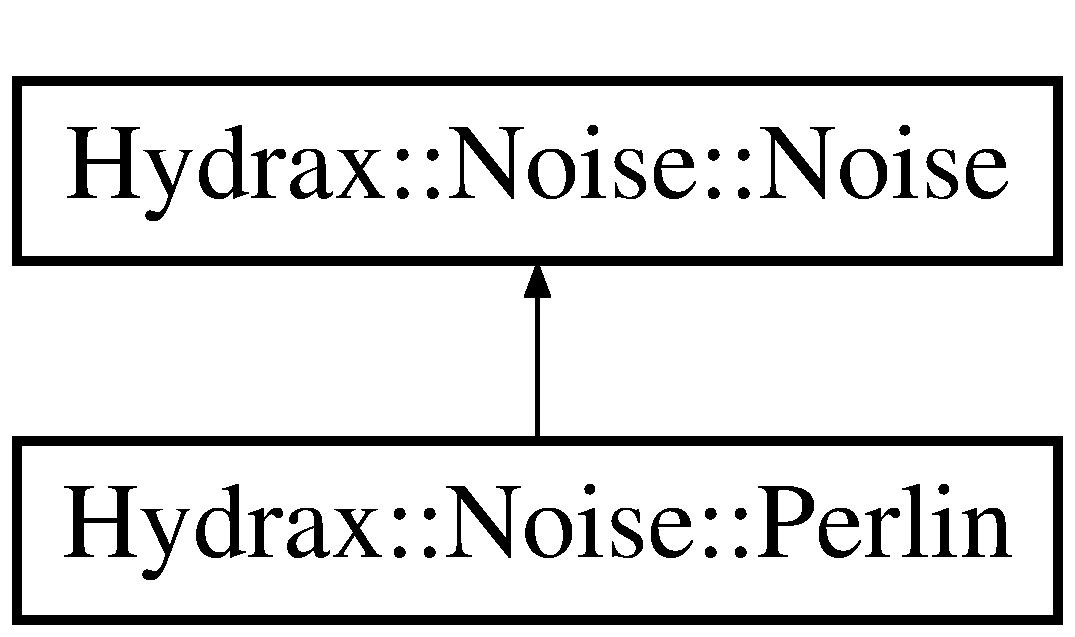
\includegraphics[height=2cm]{class_hydrax_1_1_noise_1_1_perlin}
\end{center}
\end{figure}
\subsection*{Classes}
\begin{CompactItemize}
\item 
struct \hyperlink{struct_hydrax_1_1_noise_1_1_perlin_1_1_options}{Options}
\end{CompactItemize}
\subsection*{Public Member Functions}
\begin{CompactItemize}
\item 
\hyperlink{class_hydrax_1_1_noise_1_1_perlin_65eccde5668e55133aef2f57f02613c2}{Perlin} ()
\item 
\hyperlink{class_hydrax_1_1_noise_1_1_perlin_363743192e0e9e9ab8bc4ff9f771e06c}{Perlin} (const \hyperlink{struct_hydrax_1_1_noise_1_1_perlin_1_1_options}{Options} \&\hyperlink{struct_hydrax_1_1_noise_1_1_perlin_1_1_options}{Options})
\item 
\hyperlink{class_hydrax_1_1_noise_1_1_perlin_472506339005ea5196846d26bb8fd4c1}{$\sim$Perlin} ()
\item 
void \hyperlink{class_hydrax_1_1_noise_1_1_perlin_3e260e7c239d90da210aa3e27289c6f0}{create} ()
\item 
void \hyperlink{class_hydrax_1_1_noise_1_1_perlin_666010a5142bbb2b03c97aa5aa7bdef1}{remove} ()
\item 
bool \hyperlink{class_hydrax_1_1_noise_1_1_perlin_db347b98692bd7ce6ad7ce76c605d15a}{createGPUNormalMapResources} (\hyperlink{class_hydrax_1_1_g_p_u_normal_map_manager}{GPUNormalMapManager} $\ast$g)
\item 
void \hyperlink{class_hydrax_1_1_noise_1_1_perlin_2037c02fa7d577eb72487a1b778b62dd}{update} (const Ogre::Real \&timeSinceLastFrame)
\item 
void \hyperlink{class_hydrax_1_1_noise_1_1_perlin_4f1f70a3375ac2b2f5e09011e7cc7ef3}{saveCfg} (Ogre::String \&Data)
\item 
bool \hyperlink{class_hydrax_1_1_noise_1_1_perlin_3a2dab14cfbda1ccf8fc5de4bb89f124}{loadCfg} (Ogre::ConfigFile \&CfgFile)
\item 
float \hyperlink{class_hydrax_1_1_noise_1_1_perlin_64bbe19643e0a87c08c62d0e73d7aac6}{getValue} (const float \&x, const float \&y)
\item 
void \hyperlink{class_hydrax_1_1_noise_1_1_perlin_f32b1054557536eb5073e9ad1251a4cf}{setOptions} (const \hyperlink{struct_hydrax_1_1_noise_1_1_perlin_1_1_options}{Options} \&\hyperlink{struct_hydrax_1_1_noise_1_1_perlin_1_1_options}{Options})
\item 
const \hyperlink{struct_hydrax_1_1_noise_1_1_perlin_1_1_options}{Options} \& \hyperlink{class_hydrax_1_1_noise_1_1_perlin_9264b637fe60ec9edf77c5e64881a62f}{getOptions} () const 
\end{CompactItemize}


\subsection{Detailed Description}
\hyperlink{class_hydrax_1_1_noise_1_1_perlin}{Perlin} noise module class 

\subsection{Constructor \& Destructor Documentation}
\hypertarget{class_hydrax_1_1_noise_1_1_perlin_65eccde5668e55133aef2f57f02613c2}{
\index{Hydrax::Noise::Perlin@{Hydrax::Noise::Perlin}!Perlin@{Perlin}}
\index{Perlin@{Perlin}!Hydrax::Noise::Perlin@{Hydrax::Noise::Perlin}}
\subsubsection[{Perlin}]{\setlength{\rightskip}{0pt plus 5cm}Hydrax::Noise::Perlin::Perlin ()}}
\label{class_hydrax_1_1_noise_1_1_perlin_65eccde5668e55133aef2f57f02613c2}


Default constructor \hypertarget{class_hydrax_1_1_noise_1_1_perlin_363743192e0e9e9ab8bc4ff9f771e06c}{
\index{Hydrax::Noise::Perlin@{Hydrax::Noise::Perlin}!Perlin@{Perlin}}
\index{Perlin@{Perlin}!Hydrax::Noise::Perlin@{Hydrax::Noise::Perlin}}
\subsubsection[{Perlin}]{\setlength{\rightskip}{0pt plus 5cm}Hydrax::Noise::Perlin::Perlin (const {\bf Options} \& {\em Options})}}
\label{class_hydrax_1_1_noise_1_1_perlin_363743192e0e9e9ab8bc4ff9f771e06c}


Constructor \begin{Desc}
\item[Parameters:]
\begin{description}
\item[{\em \hyperlink{struct_hydrax_1_1_noise_1_1_perlin_1_1_options}{Options}}]\hyperlink{class_hydrax_1_1_noise_1_1_perlin}{Perlin} noise options \end{description}
\end{Desc}
\hypertarget{class_hydrax_1_1_noise_1_1_perlin_472506339005ea5196846d26bb8fd4c1}{
\index{Hydrax::Noise::Perlin@{Hydrax::Noise::Perlin}!$\sim$Perlin@{$\sim$Perlin}}
\index{$\sim$Perlin@{$\sim$Perlin}!Hydrax::Noise::Perlin@{Hydrax::Noise::Perlin}}
\subsubsection[{$\sim$Perlin}]{\setlength{\rightskip}{0pt plus 5cm}Hydrax::Noise::Perlin::$\sim$Perlin ()}}
\label{class_hydrax_1_1_noise_1_1_perlin_472506339005ea5196846d26bb8fd4c1}


Destructor 

\subsection{Member Function Documentation}
\hypertarget{class_hydrax_1_1_noise_1_1_perlin_3e260e7c239d90da210aa3e27289c6f0}{
\index{Hydrax::Noise::Perlin@{Hydrax::Noise::Perlin}!create@{create}}
\index{create@{create}!Hydrax::Noise::Perlin@{Hydrax::Noise::Perlin}}
\subsubsection[{create}]{\setlength{\rightskip}{0pt plus 5cm}void Hydrax::Noise::Perlin::create ()\hspace{0.3cm}{\tt  \mbox{[}virtual\mbox{]}}}}
\label{class_hydrax_1_1_noise_1_1_perlin_3e260e7c239d90da210aa3e27289c6f0}


Create 

Reimplemented from \hyperlink{class_hydrax_1_1_noise_1_1_noise_be9cf8765feed765e6a35b0779125f6a}{Hydrax::Noise::Noise}.\hypertarget{class_hydrax_1_1_noise_1_1_perlin_db347b98692bd7ce6ad7ce76c605d15a}{
\index{Hydrax::Noise::Perlin@{Hydrax::Noise::Perlin}!createGPUNormalMapResources@{createGPUNormalMapResources}}
\index{createGPUNormalMapResources@{createGPUNormalMapResources}!Hydrax::Noise::Perlin@{Hydrax::Noise::Perlin}}
\subsubsection[{createGPUNormalMapResources}]{\setlength{\rightskip}{0pt plus 5cm}bool Hydrax::Noise::Perlin::createGPUNormalMapResources ({\bf GPUNormalMapManager} $\ast$ {\em g})\hspace{0.3cm}{\tt  \mbox{[}virtual\mbox{]}}}}
\label{class_hydrax_1_1_noise_1_1_perlin_db347b98692bd7ce6ad7ce76c605d15a}


Create GPUNormalMap resources \begin{Desc}
\item[Parameters:]
\begin{description}
\item[{\em g}]\hyperlink{class_hydrax_1_1_g_p_u_normal_map_manager}{GPUNormalMapManager} pointer \end{description}
\end{Desc}
\begin{Desc}
\item[Returns:]true if it needs to be created, false if not \end{Desc}


Reimplemented from \hyperlink{class_hydrax_1_1_noise_1_1_noise_59f0e03e88a5de69065838adc35ff2d8}{Hydrax::Noise::Noise}.\hypertarget{class_hydrax_1_1_noise_1_1_perlin_9264b637fe60ec9edf77c5e64881a62f}{
\index{Hydrax::Noise::Perlin@{Hydrax::Noise::Perlin}!getOptions@{getOptions}}
\index{getOptions@{getOptions}!Hydrax::Noise::Perlin@{Hydrax::Noise::Perlin}}
\subsubsection[{getOptions}]{\setlength{\rightskip}{0pt plus 5cm}const {\bf Options}\& Hydrax::Noise::Perlin::getOptions () const\hspace{0.3cm}{\tt  \mbox{[}inline\mbox{]}}}}
\label{class_hydrax_1_1_noise_1_1_perlin_9264b637fe60ec9edf77c5e64881a62f}


Get current \hyperlink{class_hydrax_1_1_noise_1_1_perlin}{Perlin} noise options \begin{Desc}
\item[Returns:]Current perlin noise options \end{Desc}
\hypertarget{class_hydrax_1_1_noise_1_1_perlin_64bbe19643e0a87c08c62d0e73d7aac6}{
\index{Hydrax::Noise::Perlin@{Hydrax::Noise::Perlin}!getValue@{getValue}}
\index{getValue@{getValue}!Hydrax::Noise::Perlin@{Hydrax::Noise::Perlin}}
\subsubsection[{getValue}]{\setlength{\rightskip}{0pt plus 5cm}float Hydrax::Noise::Perlin::getValue (const float \& {\em x}, \/  const float \& {\em y})\hspace{0.3cm}{\tt  \mbox{[}virtual\mbox{]}}}}
\label{class_hydrax_1_1_noise_1_1_perlin_64bbe19643e0a87c08c62d0e73d7aac6}


Get the especified x/y noise value \begin{Desc}
\item[Parameters:]
\begin{description}
\item[{\em x}]X Coord \item[{\em y}]Y Coord \end{description}
\end{Desc}
\begin{Desc}
\item[Returns:]\hyperlink{class_hydrax_1_1_noise_1_1_noise}{Noise} value \end{Desc}
\begin{Desc}
\item[Remarks:]range \mbox{[}$\sim$-0.2, $\sim$0.2\mbox{]} \end{Desc}


Implements \hyperlink{class_hydrax_1_1_noise_1_1_noise_5b18138d5c2c5ea3c3659cef80dd3a3e}{Hydrax::Noise::Noise}.\hypertarget{class_hydrax_1_1_noise_1_1_perlin_3a2dab14cfbda1ccf8fc5de4bb89f124}{
\index{Hydrax::Noise::Perlin@{Hydrax::Noise::Perlin}!loadCfg@{loadCfg}}
\index{loadCfg@{loadCfg}!Hydrax::Noise::Perlin@{Hydrax::Noise::Perlin}}
\subsubsection[{loadCfg}]{\setlength{\rightskip}{0pt plus 5cm}bool Hydrax::Noise::Perlin::loadCfg (Ogre::ConfigFile \& {\em CfgFile})\hspace{0.3cm}{\tt  \mbox{[}virtual\mbox{]}}}}
\label{class_hydrax_1_1_noise_1_1_perlin_3a2dab14cfbda1ccf8fc5de4bb89f124}


Load config \begin{Desc}
\item[Parameters:]
\begin{description}
\item[{\em CgfFile}]Ogre::ConfigFile reference \end{description}
\end{Desc}
\begin{Desc}
\item[Returns:]True if is the correct noise config \end{Desc}


Reimplemented from \hyperlink{class_hydrax_1_1_noise_1_1_noise_5ef6e71282a9dfcefc09e3ba84a7578f}{Hydrax::Noise::Noise}.\hypertarget{class_hydrax_1_1_noise_1_1_perlin_666010a5142bbb2b03c97aa5aa7bdef1}{
\index{Hydrax::Noise::Perlin@{Hydrax::Noise::Perlin}!remove@{remove}}
\index{remove@{remove}!Hydrax::Noise::Perlin@{Hydrax::Noise::Perlin}}
\subsubsection[{remove}]{\setlength{\rightskip}{0pt plus 5cm}void Hydrax::Noise::Perlin::remove ()\hspace{0.3cm}{\tt  \mbox{[}virtual\mbox{]}}}}
\label{class_hydrax_1_1_noise_1_1_perlin_666010a5142bbb2b03c97aa5aa7bdef1}


Remove 

Reimplemented from \hyperlink{class_hydrax_1_1_noise_1_1_noise_00c4aaa7604ea492740318d01f651606}{Hydrax::Noise::Noise}.\hypertarget{class_hydrax_1_1_noise_1_1_perlin_4f1f70a3375ac2b2f5e09011e7cc7ef3}{
\index{Hydrax::Noise::Perlin@{Hydrax::Noise::Perlin}!saveCfg@{saveCfg}}
\index{saveCfg@{saveCfg}!Hydrax::Noise::Perlin@{Hydrax::Noise::Perlin}}
\subsubsection[{saveCfg}]{\setlength{\rightskip}{0pt plus 5cm}void Hydrax::Noise::Perlin::saveCfg (Ogre::String \& {\em Data})\hspace{0.3cm}{\tt  \mbox{[}virtual\mbox{]}}}}
\label{class_hydrax_1_1_noise_1_1_perlin_4f1f70a3375ac2b2f5e09011e7cc7ef3}


Save config \begin{Desc}
\item[Parameters:]
\begin{description}
\item[{\em Data}]String reference \end{description}
\end{Desc}


Reimplemented from \hyperlink{class_hydrax_1_1_noise_1_1_noise_ac0a9fe1533ddd87467edb954f8abea8}{Hydrax::Noise::Noise}.\hypertarget{class_hydrax_1_1_noise_1_1_perlin_f32b1054557536eb5073e9ad1251a4cf}{
\index{Hydrax::Noise::Perlin@{Hydrax::Noise::Perlin}!setOptions@{setOptions}}
\index{setOptions@{setOptions}!Hydrax::Noise::Perlin@{Hydrax::Noise::Perlin}}
\subsubsection[{setOptions}]{\setlength{\rightskip}{0pt plus 5cm}void Hydrax::Noise::Perlin::setOptions (const {\bf Options} \& {\em Options})}}
\label{class_hydrax_1_1_noise_1_1_perlin_f32b1054557536eb5073e9ad1251a4cf}


Set/Update perlin noise options \begin{Desc}
\item[Parameters:]
\begin{description}
\item[{\em \hyperlink{struct_hydrax_1_1_noise_1_1_perlin_1_1_options}{Options}}]\hyperlink{class_hydrax_1_1_noise_1_1_perlin}{Perlin} noise options \end{description}
\end{Desc}
\begin{Desc}
\item[Remarks:]If \hyperlink{class_hydrax_1_1_noise_1_1_perlin_3e260e7c239d90da210aa3e27289c6f0}{create()} have been already called, Octaves option doesn't be updated. \end{Desc}
\hypertarget{class_hydrax_1_1_noise_1_1_perlin_2037c02fa7d577eb72487a1b778b62dd}{
\index{Hydrax::Noise::Perlin@{Hydrax::Noise::Perlin}!update@{update}}
\index{update@{update}!Hydrax::Noise::Perlin@{Hydrax::Noise::Perlin}}
\subsubsection[{update}]{\setlength{\rightskip}{0pt plus 5cm}void Hydrax::Noise::Perlin::update (const Ogre::Real \& {\em timeSinceLastFrame})\hspace{0.3cm}{\tt  \mbox{[}virtual\mbox{]}}}}
\label{class_hydrax_1_1_noise_1_1_perlin_2037c02fa7d577eb72487a1b778b62dd}


Call it each frame \begin{Desc}
\item[Parameters:]
\begin{description}
\item[{\em timeSinceLastFrame}]Time since last frame(delta) \end{description}
\end{Desc}


Implements \hyperlink{class_hydrax_1_1_noise_1_1_noise_9c32c4c630f193e034c074f69ea10f57}{Hydrax::Noise::Noise}.

The documentation for this class was generated from the following files:\begin{CompactItemize}
\item 
C:/Hydrax/v0.5.1/Hydrax/src/Hydrax/Noise/Perlin/\hyperlink{_perlin_8h}{Perlin.h}\item 
C:/Hydrax/v0.5.1/Hydrax/src/Hydrax/Noise/Perlin/\hyperlink{_perlin_8cpp}{Perlin.cpp}\end{CompactItemize}

\hypertarget{struct_hydrax_1_1_noise_1_1_perlin_1_1_options}{
\section{Hydrax::Noise::Perlin::Perlin::Options Struct Reference}
\label{struct_hydrax_1_1_noise_1_1_perlin_1_1_options}\index{Hydrax::Noise::Perlin::Options@{Hydrax::Noise::Perlin::Options}}
}
{\tt \#include $<$Perlin.h$>$}

\subsection*{Public Member Functions}
\begin{CompactItemize}
\item 
\hyperlink{struct_hydrax_1_1_noise_1_1_perlin_1_1_options_357458115476a5b0b9ba11060fb345df}{Options} ()
\item 
\hyperlink{struct_hydrax_1_1_noise_1_1_perlin_1_1_options_83c9cc814d0713f1424fbf1e7e4b2f70}{Options} (const int \&\_\-Octaves, const float \&\_\-Scale, const float \&\_\-Falloff, const float \&\_\-Animspeed, const float \&\_\-Timemulti)
\item 
\hyperlink{struct_hydrax_1_1_noise_1_1_perlin_1_1_options_be063c5cb7eba48426af6edced02fc15}{Options} (const int \&\_\-Octaves, const float \&\_\-Scale, const float \&\_\-Falloff, const float \&\_\-Animspeed, const float \&\_\-Timemulti, const float \&\_\-GPU\_\-Strength, const Ogre::Vector3 \&\_\-GPU\_\-LODParameters)
\end{CompactItemize}
\subsection*{Public Attributes}
\begin{CompactItemize}
\item 
int \hyperlink{struct_hydrax_1_1_noise_1_1_perlin_1_1_options_619c2288fa73c1bae98e475cff6c3e26}{Octaves}
\begin{CompactList}\small\item\em Octaves. \item\end{CompactList}\item 
float \hyperlink{struct_hydrax_1_1_noise_1_1_perlin_1_1_options_06e7bb58600f974065a2d2bdcd6a9f91}{Scale}
\begin{CompactList}\small\item\em Scale. \item\end{CompactList}\item 
float \hyperlink{struct_hydrax_1_1_noise_1_1_perlin_1_1_options_8fdaf68802a6abfa74665e8fd31a54aa}{Falloff}
\begin{CompactList}\small\item\em Falloff. \item\end{CompactList}\item 
float \hyperlink{struct_hydrax_1_1_noise_1_1_perlin_1_1_options_77f9a42f5ebbe148f0c4610f3fe818cd}{Animspeed}
\begin{CompactList}\small\item\em Animspeed. \item\end{CompactList}\item 
float \hyperlink{struct_hydrax_1_1_noise_1_1_perlin_1_1_options_7619c42d9f43aa51d26dd954d56b17c3}{Timemulti}
\begin{CompactList}\small\item\em Timemulti. \item\end{CompactList}\item 
float \hyperlink{struct_hydrax_1_1_noise_1_1_perlin_1_1_options_2c4f7deaf01fdb818adde19b1174c48d}{GPU\_\-Strength}
\begin{CompactList}\small\item\em Representes the strength of the normals (i.e. Amplitude). \item\end{CompactList}\item 
Ogre::Vector3 \hyperlink{struct_hydrax_1_1_noise_1_1_perlin_1_1_options_8abb72bf1ee4792f2627f6bc635d7aa2}{GPU\_\-LODParameters}
\end{CompactItemize}


\subsection{Detailed Description}
Struct wich contains \hyperlink{class_hydrax_1_1_noise_1_1_perlin}{Perlin} noise module options 

\subsection{Constructor \& Destructor Documentation}
\hypertarget{struct_hydrax_1_1_noise_1_1_perlin_1_1_options_357458115476a5b0b9ba11060fb345df}{
\index{Hydrax::Noise::Perlin::Options@{Hydrax::Noise::Perlin::Options}!Options@{Options}}
\index{Options@{Options}!Hydrax::Noise::Perlin::Options@{Hydrax::Noise::Perlin::Options}}
\subsubsection[{Options}]{\setlength{\rightskip}{0pt plus 5cm}Hydrax::Noise::Perlin::Perlin::Options::Options ()\hspace{0.3cm}{\tt  \mbox{[}inline\mbox{]}}}}
\label{struct_hydrax_1_1_noise_1_1_perlin_1_1_options_357458115476a5b0b9ba11060fb345df}


Default constructor \hypertarget{struct_hydrax_1_1_noise_1_1_perlin_1_1_options_83c9cc814d0713f1424fbf1e7e4b2f70}{
\index{Hydrax::Noise::Perlin::Options@{Hydrax::Noise::Perlin::Options}!Options@{Options}}
\index{Options@{Options}!Hydrax::Noise::Perlin::Options@{Hydrax::Noise::Perlin::Options}}
\subsubsection[{Options}]{\setlength{\rightskip}{0pt plus 5cm}Hydrax::Noise::Perlin::Perlin::Options::Options (const int \& {\em \_\-Octaves}, \/  const float \& {\em \_\-Scale}, \/  const float \& {\em \_\-Falloff}, \/  const float \& {\em \_\-Animspeed}, \/  const float \& {\em \_\-Timemulti})\hspace{0.3cm}{\tt  \mbox{[}inline\mbox{]}}}}
\label{struct_hydrax_1_1_noise_1_1_perlin_1_1_options_83c9cc814d0713f1424fbf1e7e4b2f70}


Constructor \begin{Desc}
\item[Parameters:]
\begin{description}
\item[{\em \_\-Octaves}]\hyperlink{class_hydrax_1_1_noise_1_1_perlin}{Perlin} noise octaves \item[{\em \_\-Scale}]\hyperlink{class_hydrax_1_1_noise_1_1_noise}{Noise} scale \item[{\em \_\-Falloff}]\hyperlink{class_hydrax_1_1_noise_1_1_noise}{Noise} fall off \item[{\em \_\-Animspeed}]Animation speed \item[{\em \_\-Timemulti}]Timemulti \end{description}
\end{Desc}
\hypertarget{struct_hydrax_1_1_noise_1_1_perlin_1_1_options_be063c5cb7eba48426af6edced02fc15}{
\index{Hydrax::Noise::Perlin::Options@{Hydrax::Noise::Perlin::Options}!Options@{Options}}
\index{Options@{Options}!Hydrax::Noise::Perlin::Options@{Hydrax::Noise::Perlin::Options}}
\subsubsection[{Options}]{\setlength{\rightskip}{0pt plus 5cm}Hydrax::Noise::Perlin::Perlin::Options::Options (const int \& {\em \_\-Octaves}, \/  const float \& {\em \_\-Scale}, \/  const float \& {\em \_\-Falloff}, \/  const float \& {\em \_\-Animspeed}, \/  const float \& {\em \_\-Timemulti}, \/  const float \& {\em \_\-GPU\_\-Strength}, \/  const Ogre::Vector3 \& {\em \_\-GPU\_\-LODParameters})\hspace{0.3cm}{\tt  \mbox{[}inline\mbox{]}}}}
\label{struct_hydrax_1_1_noise_1_1_perlin_1_1_options_be063c5cb7eba48426af6edced02fc15}


Constructor \begin{Desc}
\item[Parameters:]
\begin{description}
\item[{\em \_\-Octaves}]\hyperlink{class_hydrax_1_1_noise_1_1_perlin}{Perlin} noise octaves \item[{\em \_\-Scale}]\hyperlink{class_hydrax_1_1_noise_1_1_noise}{Noise} scale \item[{\em \_\-Falloff}]\hyperlink{class_hydrax_1_1_noise_1_1_noise}{Noise} fall off \item[{\em \_\-Animspeed}]Animation speed \item[{\em \_\-Timemulti}]Timemulti \item[{\em \_\-GPU\_\-Strength}]GPU\_\-Strength \item[{\em \_\-GPU\_\-LODParameters}]GPU\_\-LODParameters \end{description}
\end{Desc}


\subsection{Member Data Documentation}
\hypertarget{struct_hydrax_1_1_noise_1_1_perlin_1_1_options_77f9a42f5ebbe148f0c4610f3fe818cd}{
\index{Hydrax::Noise::Perlin::Options@{Hydrax::Noise::Perlin::Options}!Animspeed@{Animspeed}}
\index{Animspeed@{Animspeed}!Hydrax::Noise::Perlin::Options@{Hydrax::Noise::Perlin::Options}}
\subsubsection[{Animspeed}]{\setlength{\rightskip}{0pt plus 5cm}float Hydrax::Noise::Perlin::Perlin::Options::Animspeed}}
\label{struct_hydrax_1_1_noise_1_1_perlin_1_1_options_77f9a42f5ebbe148f0c4610f3fe818cd}


Animspeed. 

\hypertarget{struct_hydrax_1_1_noise_1_1_perlin_1_1_options_8fdaf68802a6abfa74665e8fd31a54aa}{
\index{Hydrax::Noise::Perlin::Options@{Hydrax::Noise::Perlin::Options}!Falloff@{Falloff}}
\index{Falloff@{Falloff}!Hydrax::Noise::Perlin::Options@{Hydrax::Noise::Perlin::Options}}
\subsubsection[{Falloff}]{\setlength{\rightskip}{0pt plus 5cm}float Hydrax::Noise::Perlin::Perlin::Options::Falloff}}
\label{struct_hydrax_1_1_noise_1_1_perlin_1_1_options_8fdaf68802a6abfa74665e8fd31a54aa}


Falloff. 

\hypertarget{struct_hydrax_1_1_noise_1_1_perlin_1_1_options_8abb72bf1ee4792f2627f6bc635d7aa2}{
\index{Hydrax::Noise::Perlin::Options@{Hydrax::Noise::Perlin::Options}!GPU\_\-LODParameters@{GPU\_\-LODParameters}}
\index{GPU\_\-LODParameters@{GPU\_\-LODParameters}!Hydrax::Noise::Perlin::Options@{Hydrax::Noise::Perlin::Options}}
\subsubsection[{GPU\_\-LODParameters}]{\setlength{\rightskip}{0pt plus 5cm}Ogre::Vector3 Hydrax::Noise::Perlin::Perlin::Options::GPU\_\-LODParameters}}
\label{struct_hydrax_1_1_noise_1_1_perlin_1_1_options_8abb72bf1ee4792f2627f6bc635d7aa2}


LOD Parameters, in order to obtain a smooth normal map we need to decrease the detail level when the pixel is far to the camera. This parameters are stored in an Ogre::Vector3: x -$>$ Initial LOD value (Bigger values -$>$ less detail) y -$>$ Final LOD value z -$>$ Final distance \hypertarget{struct_hydrax_1_1_noise_1_1_perlin_1_1_options_2c4f7deaf01fdb818adde19b1174c48d}{
\index{Hydrax::Noise::Perlin::Options@{Hydrax::Noise::Perlin::Options}!GPU\_\-Strength@{GPU\_\-Strength}}
\index{GPU\_\-Strength@{GPU\_\-Strength}!Hydrax::Noise::Perlin::Options@{Hydrax::Noise::Perlin::Options}}
\subsubsection[{GPU\_\-Strength}]{\setlength{\rightskip}{0pt plus 5cm}float Hydrax::Noise::Perlin::Perlin::Options::GPU\_\-Strength}}
\label{struct_hydrax_1_1_noise_1_1_perlin_1_1_options_2c4f7deaf01fdb818adde19b1174c48d}


Representes the strength of the normals (i.e. Amplitude). 

GPU Normal map generator parameters Only if GPU normal map generation is active \hypertarget{struct_hydrax_1_1_noise_1_1_perlin_1_1_options_619c2288fa73c1bae98e475cff6c3e26}{
\index{Hydrax::Noise::Perlin::Options@{Hydrax::Noise::Perlin::Options}!Octaves@{Octaves}}
\index{Octaves@{Octaves}!Hydrax::Noise::Perlin::Options@{Hydrax::Noise::Perlin::Options}}
\subsubsection[{Octaves}]{\setlength{\rightskip}{0pt plus 5cm}int Hydrax::Noise::Perlin::Perlin::Options::Octaves}}
\label{struct_hydrax_1_1_noise_1_1_perlin_1_1_options_619c2288fa73c1bae98e475cff6c3e26}


Octaves. 

\hypertarget{struct_hydrax_1_1_noise_1_1_perlin_1_1_options_06e7bb58600f974065a2d2bdcd6a9f91}{
\index{Hydrax::Noise::Perlin::Options@{Hydrax::Noise::Perlin::Options}!Scale@{Scale}}
\index{Scale@{Scale}!Hydrax::Noise::Perlin::Options@{Hydrax::Noise::Perlin::Options}}
\subsubsection[{Scale}]{\setlength{\rightskip}{0pt plus 5cm}float Hydrax::Noise::Perlin::Perlin::Options::Scale}}
\label{struct_hydrax_1_1_noise_1_1_perlin_1_1_options_06e7bb58600f974065a2d2bdcd6a9f91}


Scale. 

\hypertarget{struct_hydrax_1_1_noise_1_1_perlin_1_1_options_7619c42d9f43aa51d26dd954d56b17c3}{
\index{Hydrax::Noise::Perlin::Options@{Hydrax::Noise::Perlin::Options}!Timemulti@{Timemulti}}
\index{Timemulti@{Timemulti}!Hydrax::Noise::Perlin::Options@{Hydrax::Noise::Perlin::Options}}
\subsubsection[{Timemulti}]{\setlength{\rightskip}{0pt plus 5cm}float Hydrax::Noise::Perlin::Perlin::Options::Timemulti}}
\label{struct_hydrax_1_1_noise_1_1_perlin_1_1_options_7619c42d9f43aa51d26dd954d56b17c3}


Timemulti. 



The documentation for this struct was generated from the following file:\begin{CompactItemize}
\item 
C:/Hydrax/v0.5.1/Hydrax/src/Hydrax/Noise/Perlin/\hyperlink{_perlin_8h}{Perlin.h}\end{CompactItemize}

\hypertarget{class_hydrax_1_1_module_1_1_projected_grid}{
\section{Hydrax::Module::ProjectedGrid Class Reference}
\label{class_hydrax_1_1_module_1_1_projected_grid}\index{Hydrax::Module::ProjectedGrid@{Hydrax::Module::ProjectedGrid}}
}
{\tt \#include $<$ProjectedGrid.h$>$}

Inheritance diagram for Hydrax::Module::ProjectedGrid::\begin{figure}[H]
\begin{center}
\leavevmode
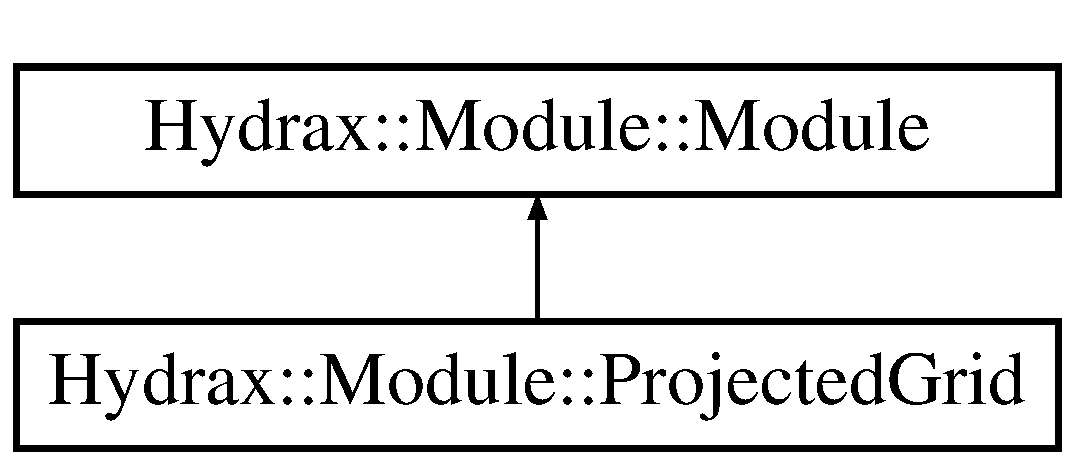
\includegraphics[height=2cm]{class_hydrax_1_1_module_1_1_projected_grid}
\end{center}
\end{figure}
\subsection*{Classes}
\begin{CompactItemize}
\item 
struct \hyperlink{struct_hydrax_1_1_module_1_1_projected_grid_1_1_options}{Options}
\end{CompactItemize}
\subsection*{Public Member Functions}
\begin{CompactItemize}
\item 
\hyperlink{class_hydrax_1_1_module_1_1_projected_grid_ccda1b1a4c84e3da9b8a96e7dcb69a27}{ProjectedGrid} (\hyperlink{class_hydrax_1_1_hydrax}{Hydrax} $\ast$h, \hyperlink{class_hydrax_1_1_noise_1_1_noise}{Noise::Noise} $\ast$n, const Ogre::Plane \&BasePlane, const \hyperlink{class_hydrax_1_1_material_manager_aa14689cd1c259f48954dfecda9b296f}{MaterialManager::NormalMode} \&NormalMode)
\item 
\hyperlink{class_hydrax_1_1_module_1_1_projected_grid_a9308990b99866cbd09edd3600972443}{ProjectedGrid} (\hyperlink{class_hydrax_1_1_hydrax}{Hydrax} $\ast$h, \hyperlink{class_hydrax_1_1_noise_1_1_noise}{Noise::Noise} $\ast$n, const Ogre::Plane \&BasePlane, const \hyperlink{class_hydrax_1_1_material_manager_aa14689cd1c259f48954dfecda9b296f}{MaterialManager::NormalMode} \&NormalMode, const \hyperlink{struct_hydrax_1_1_module_1_1_projected_grid_1_1_options}{Options} \&\hyperlink{struct_hydrax_1_1_module_1_1_projected_grid_1_1_options}{Options})
\item 
\hyperlink{class_hydrax_1_1_module_1_1_projected_grid_7b656225a58519ec687225f1f809010c}{$\sim$ProjectedGrid} ()
\item 
void \hyperlink{class_hydrax_1_1_module_1_1_projected_grid_86e4648a741558934e664f7400082742}{create} ()
\item 
void \hyperlink{class_hydrax_1_1_module_1_1_projected_grid_b878b7d1258aacda8bee0f2e945ea64d}{remove} ()
\item 
void \hyperlink{class_hydrax_1_1_module_1_1_projected_grid_8d7a8efcd6b7fd0e4313c9114bd2c061}{update} (const Ogre::Real \&timeSinceLastFrame)
\item 
void \hyperlink{class_hydrax_1_1_module_1_1_projected_grid_04d04b9cfc173538038a5f51094c1ffa}{setOptions} (const \hyperlink{struct_hydrax_1_1_module_1_1_projected_grid_1_1_options}{Options} \&\hyperlink{struct_hydrax_1_1_module_1_1_projected_grid_1_1_options}{Options})
\item 
void \hyperlink{class_hydrax_1_1_module_1_1_projected_grid_4502387739439e0d6cca1f006fc4a28c}{saveCfg} (Ogre::String \&Data)
\item 
bool \hyperlink{class_hydrax_1_1_module_1_1_projected_grid_f951c58cc93cf75d57e69aa14a668d3e}{loadCfg} (Ogre::ConfigFile \&CfgFile)
\item 
float \hyperlink{class_hydrax_1_1_module_1_1_projected_grid_a7a5b8100642a55f23b4d1c0a125bd62}{getHeigth} (const Ogre::Vector2 \&Position)
\item 
const \hyperlink{struct_hydrax_1_1_module_1_1_projected_grid_1_1_options}{Options} \& \hyperlink{class_hydrax_1_1_module_1_1_projected_grid_0a0aaa55436af95f5cf16aa284d24f57}{getOptions} () const 
\end{CompactItemize}


\subsection{Detailed Description}
\hyperlink{class_hydrax_1_1_hydrax}{Hydrax} projected grid module 

\subsection{Constructor \& Destructor Documentation}
\hypertarget{class_hydrax_1_1_module_1_1_projected_grid_ccda1b1a4c84e3da9b8a96e7dcb69a27}{
\index{Hydrax::Module::ProjectedGrid@{Hydrax::Module::ProjectedGrid}!ProjectedGrid@{ProjectedGrid}}
\index{ProjectedGrid@{ProjectedGrid}!Hydrax::Module::ProjectedGrid@{Hydrax::Module::ProjectedGrid}}
\subsubsection[{ProjectedGrid}]{\setlength{\rightskip}{0pt plus 5cm}Hydrax::Module::ProjectedGrid::ProjectedGrid ({\bf Hydrax} $\ast$ {\em h}, \/  {\bf Noise::Noise} $\ast$ {\em n}, \/  const Ogre::Plane \& {\em BasePlane}, \/  const {\bf MaterialManager::NormalMode} \& {\em NormalMode})}}
\label{class_hydrax_1_1_module_1_1_projected_grid_ccda1b1a4c84e3da9b8a96e7dcb69a27}


Constructor \begin{Desc}
\item[Parameters:]
\begin{description}
\item[{\em h}]\hyperlink{class_hydrax_1_1_hydrax}{Hydrax} manager pointer \item[{\em n}]\hyperlink{class_hydrax_1_1_hydrax}{Hydrax} noise module \item[{\em BasePlane}]\hyperlink{namespace_hydrax_1_1_noise}{Noise} base plane \item[{\em NormalMode}]Switch between \hyperlink{class_hydrax_1_1_material_manager_aa14689cd1c259f48954dfecda9b296ffe4d6257f673cf503a9905fb2576288f}{MaterialManager::NM\_\-VERTEX} and Materialmanager::NM\_\-RTT \end{description}
\end{Desc}
\hypertarget{class_hydrax_1_1_module_1_1_projected_grid_a9308990b99866cbd09edd3600972443}{
\index{Hydrax::Module::ProjectedGrid@{Hydrax::Module::ProjectedGrid}!ProjectedGrid@{ProjectedGrid}}
\index{ProjectedGrid@{ProjectedGrid}!Hydrax::Module::ProjectedGrid@{Hydrax::Module::ProjectedGrid}}
\subsubsection[{ProjectedGrid}]{\setlength{\rightskip}{0pt plus 5cm}Hydrax::Module::ProjectedGrid::ProjectedGrid ({\bf Hydrax} $\ast$ {\em h}, \/  {\bf Noise::Noise} $\ast$ {\em n}, \/  const Ogre::Plane \& {\em BasePlane}, \/  const {\bf MaterialManager::NormalMode} \& {\em NormalMode}, \/  const {\bf Options} \& {\em Options})}}
\label{class_hydrax_1_1_module_1_1_projected_grid_a9308990b99866cbd09edd3600972443}


Constructor \begin{Desc}
\item[Parameters:]
\begin{description}
\item[{\em h}]\hyperlink{class_hydrax_1_1_hydrax}{Hydrax} manager pointer \item[{\em n}]\hyperlink{class_hydrax_1_1_hydrax}{Hydrax} noise module \item[{\em BasePlane}]\hyperlink{namespace_hydrax_1_1_noise}{Noise} base plane \item[{\em NormalMode}]Switch between \hyperlink{class_hydrax_1_1_material_manager_aa14689cd1c259f48954dfecda9b296ffe4d6257f673cf503a9905fb2576288f}{MaterialManager::NM\_\-VERTEX} and Materialmanager::NM\_\-RTT \item[{\em \hyperlink{struct_hydrax_1_1_module_1_1_projected_grid_1_1_options}{Options}}]Perlin options \end{description}
\end{Desc}
\hypertarget{class_hydrax_1_1_module_1_1_projected_grid_7b656225a58519ec687225f1f809010c}{
\index{Hydrax::Module::ProjectedGrid@{Hydrax::Module::ProjectedGrid}!$\sim$ProjectedGrid@{$\sim$ProjectedGrid}}
\index{$\sim$ProjectedGrid@{$\sim$ProjectedGrid}!Hydrax::Module::ProjectedGrid@{Hydrax::Module::ProjectedGrid}}
\subsubsection[{$\sim$ProjectedGrid}]{\setlength{\rightskip}{0pt plus 5cm}Hydrax::Module::ProjectedGrid::$\sim$ProjectedGrid ()}}
\label{class_hydrax_1_1_module_1_1_projected_grid_7b656225a58519ec687225f1f809010c}


Destructor 

\subsection{Member Function Documentation}
\hypertarget{class_hydrax_1_1_module_1_1_projected_grid_86e4648a741558934e664f7400082742}{
\index{Hydrax::Module::ProjectedGrid@{Hydrax::Module::ProjectedGrid}!create@{create}}
\index{create@{create}!Hydrax::Module::ProjectedGrid@{Hydrax::Module::ProjectedGrid}}
\subsubsection[{create}]{\setlength{\rightskip}{0pt plus 5cm}void Hydrax::Module::ProjectedGrid::create ()\hspace{0.3cm}{\tt  \mbox{[}virtual\mbox{]}}}}
\label{class_hydrax_1_1_module_1_1_projected_grid_86e4648a741558934e664f7400082742}


Create 

Reimplemented from \hyperlink{class_hydrax_1_1_module_1_1_module_4b696328c3fc1496f757e929f44f3258}{Hydrax::Module::Module}.\hypertarget{class_hydrax_1_1_module_1_1_projected_grid_a7a5b8100642a55f23b4d1c0a125bd62}{
\index{Hydrax::Module::ProjectedGrid@{Hydrax::Module::ProjectedGrid}!getHeigth@{getHeigth}}
\index{getHeigth@{getHeigth}!Hydrax::Module::ProjectedGrid@{Hydrax::Module::ProjectedGrid}}
\subsubsection[{getHeigth}]{\setlength{\rightskip}{0pt plus 5cm}float Hydrax::Module::ProjectedGrid::getHeigth (const Ogre::Vector2 \& {\em Position})\hspace{0.3cm}{\tt  \mbox{[}virtual\mbox{]}}}}
\label{class_hydrax_1_1_module_1_1_projected_grid_a7a5b8100642a55f23b4d1c0a125bd62}


Get the current heigth at a especified world-space point \begin{Desc}
\item[Parameters:]
\begin{description}
\item[{\em Position}]X/Z World position \end{description}
\end{Desc}
\begin{Desc}
\item[Returns:]Heigth at the given position in y-World coordinates, if it's outside of the water return -1 \end{Desc}


Reimplemented from \hyperlink{class_hydrax_1_1_module_1_1_module_c61f89589d3b1bc7256731ddb7af7d0b}{Hydrax::Module::Module}.\hypertarget{class_hydrax_1_1_module_1_1_projected_grid_0a0aaa55436af95f5cf16aa284d24f57}{
\index{Hydrax::Module::ProjectedGrid@{Hydrax::Module::ProjectedGrid}!getOptions@{getOptions}}
\index{getOptions@{getOptions}!Hydrax::Module::ProjectedGrid@{Hydrax::Module::ProjectedGrid}}
\subsubsection[{getOptions}]{\setlength{\rightskip}{0pt plus 5cm}const {\bf Options}\& Hydrax::Module::ProjectedGrid::getOptions () const\hspace{0.3cm}{\tt  \mbox{[}inline\mbox{]}}}}
\label{class_hydrax_1_1_module_1_1_projected_grid_0a0aaa55436af95f5cf16aa284d24f57}


Get current options \begin{Desc}
\item[Returns:]Current options \end{Desc}
\hypertarget{class_hydrax_1_1_module_1_1_projected_grid_f951c58cc93cf75d57e69aa14a668d3e}{
\index{Hydrax::Module::ProjectedGrid@{Hydrax::Module::ProjectedGrid}!loadCfg@{loadCfg}}
\index{loadCfg@{loadCfg}!Hydrax::Module::ProjectedGrid@{Hydrax::Module::ProjectedGrid}}
\subsubsection[{loadCfg}]{\setlength{\rightskip}{0pt plus 5cm}bool Hydrax::Module::ProjectedGrid::loadCfg (Ogre::ConfigFile \& {\em CfgFile})\hspace{0.3cm}{\tt  \mbox{[}virtual\mbox{]}}}}
\label{class_hydrax_1_1_module_1_1_projected_grid_f951c58cc93cf75d57e69aa14a668d3e}


Load config \begin{Desc}
\item[Parameters:]
\begin{description}
\item[{\em CgfFile}]Ogre::ConfigFile reference \end{description}
\end{Desc}
\begin{Desc}
\item[Returns:]True if is the correct module config \end{Desc}


Reimplemented from \hyperlink{class_hydrax_1_1_module_1_1_module_bedb96357608c0744bb7816ae1c2b0bb}{Hydrax::Module::Module}.\hypertarget{class_hydrax_1_1_module_1_1_projected_grid_b878b7d1258aacda8bee0f2e945ea64d}{
\index{Hydrax::Module::ProjectedGrid@{Hydrax::Module::ProjectedGrid}!remove@{remove}}
\index{remove@{remove}!Hydrax::Module::ProjectedGrid@{Hydrax::Module::ProjectedGrid}}
\subsubsection[{remove}]{\setlength{\rightskip}{0pt plus 5cm}void Hydrax::Module::ProjectedGrid::remove ()\hspace{0.3cm}{\tt  \mbox{[}virtual\mbox{]}}}}
\label{class_hydrax_1_1_module_1_1_projected_grid_b878b7d1258aacda8bee0f2e945ea64d}


Remove 

Reimplemented from \hyperlink{class_hydrax_1_1_module_1_1_module_21f60a53a99d72ff00d3fe5565518165}{Hydrax::Module::Module}.\hypertarget{class_hydrax_1_1_module_1_1_projected_grid_4502387739439e0d6cca1f006fc4a28c}{
\index{Hydrax::Module::ProjectedGrid@{Hydrax::Module::ProjectedGrid}!saveCfg@{saveCfg}}
\index{saveCfg@{saveCfg}!Hydrax::Module::ProjectedGrid@{Hydrax::Module::ProjectedGrid}}
\subsubsection[{saveCfg}]{\setlength{\rightskip}{0pt plus 5cm}void Hydrax::Module::ProjectedGrid::saveCfg (Ogre::String \& {\em Data})\hspace{0.3cm}{\tt  \mbox{[}virtual\mbox{]}}}}
\label{class_hydrax_1_1_module_1_1_projected_grid_4502387739439e0d6cca1f006fc4a28c}


Save config \begin{Desc}
\item[Parameters:]
\begin{description}
\item[{\em Data}]String reference \end{description}
\end{Desc}


Reimplemented from \hyperlink{class_hydrax_1_1_module_1_1_module_998a5baf42f57b02ca7bc20bc12f95a9}{Hydrax::Module::Module}.\hypertarget{class_hydrax_1_1_module_1_1_projected_grid_04d04b9cfc173538038a5f51094c1ffa}{
\index{Hydrax::Module::ProjectedGrid@{Hydrax::Module::ProjectedGrid}!setOptions@{setOptions}}
\index{setOptions@{setOptions}!Hydrax::Module::ProjectedGrid@{Hydrax::Module::ProjectedGrid}}
\subsubsection[{setOptions}]{\setlength{\rightskip}{0pt plus 5cm}void Hydrax::Module::ProjectedGrid::setOptions (const {\bf Options} \& {\em Options})}}
\label{class_hydrax_1_1_module_1_1_projected_grid_04d04b9cfc173538038a5f51094c1ffa}


Set options \begin{Desc}
\item[Parameters:]
\begin{description}
\item[{\em \hyperlink{struct_hydrax_1_1_module_1_1_projected_grid_1_1_options}{Options}}]\hyperlink{struct_hydrax_1_1_module_1_1_projected_grid_1_1_options}{Options} \end{description}
\end{Desc}
\hypertarget{class_hydrax_1_1_module_1_1_projected_grid_8d7a8efcd6b7fd0e4313c9114bd2c061}{
\index{Hydrax::Module::ProjectedGrid@{Hydrax::Module::ProjectedGrid}!update@{update}}
\index{update@{update}!Hydrax::Module::ProjectedGrid@{Hydrax::Module::ProjectedGrid}}
\subsubsection[{update}]{\setlength{\rightskip}{0pt plus 5cm}void Hydrax::Module::ProjectedGrid::update (const Ogre::Real \& {\em timeSinceLastFrame})\hspace{0.3cm}{\tt  \mbox{[}virtual\mbox{]}}}}
\label{class_hydrax_1_1_module_1_1_projected_grid_8d7a8efcd6b7fd0e4313c9114bd2c061}


Call it each frame \begin{Desc}
\item[Parameters:]
\begin{description}
\item[{\em timeSinceLastFrame}]Time since last frame(delta) \end{description}
\end{Desc}


Reimplemented from \hyperlink{class_hydrax_1_1_module_1_1_module_2042d450f99d9348fa4b7bd29ba89df3}{Hydrax::Module::Module}.

The documentation for this class was generated from the following files:\begin{CompactItemize}
\item 
C:/Hydrax/v0.5.1/Hydrax/src/Hydrax/Modules/ProjectedGrid/\hyperlink{_projected_grid_8h}{ProjectedGrid.h}\item 
C:/Hydrax/v0.5.1/Hydrax/src/Hydrax/Modules/ProjectedGrid/\hyperlink{_projected_grid_8cpp}{ProjectedGrid.cpp}\end{CompactItemize}

\hypertarget{struct_hydrax_1_1_module_1_1_projected_grid_1_1_options}{
\section{Hydrax::Module::ProjectedGrid::ProjectedGrid::Options Struct Reference}
\label{struct_hydrax_1_1_module_1_1_projected_grid_1_1_options}\index{Hydrax::Module::ProjectedGrid::Options@{Hydrax::Module::ProjectedGrid::Options}}
}
{\tt \#include $<$ProjectedGrid.h$>$}

\subsection*{Public Member Functions}
\begin{CompactItemize}
\item 
\hyperlink{struct_hydrax_1_1_module_1_1_projected_grid_1_1_options_18aba976dbc90be89d1d4bd464f8d877}{Options} ()
\item 
\hyperlink{struct_hydrax_1_1_module_1_1_projected_grid_1_1_options_1c68747eb19c420f6b85fc4806b7c341}{Options} (const int \&\_\-Complexity)
\item 
\hyperlink{struct_hydrax_1_1_module_1_1_projected_grid_1_1_options_3c7e63596f51adb9435fcd88e9bde2b7}{Options} (const int \&\_\-Complexity, const float \&\_\-Strength, const float \&\_\-Elevation, const bool \&\_\-Smooth)
\item 
\hyperlink{struct_hydrax_1_1_module_1_1_projected_grid_1_1_options_bd3aaa3c56a7347a6c911e0c57b62be4}{Options} (const int \&\_\-Complexity, const float \&\_\-Strength, const float \&\_\-Elevation, const bool \&\_\-Smooth, const bool \&\_\-ForceRecalculateGeometry, const bool \&\_\-ChoppyWaves, const float \&\_\-ChoppyStrength)
\end{CompactItemize}
\subsection*{Public Attributes}
\begin{CompactItemize}
\item 
int \hyperlink{struct_hydrax_1_1_module_1_1_projected_grid_1_1_options_155754beb2d89d3747e930b1705d3e66}{Complexity}
\begin{CompactList}\small\item\em Projected grid complexity (N$\ast$N). \item\end{CompactList}\item 
float \hyperlink{struct_hydrax_1_1_module_1_1_projected_grid_1_1_options_d92bbf285f94fbd26a5164187c8d433b}{Strength}
\begin{CompactList}\small\item\em Strength. \item\end{CompactList}\item 
float \hyperlink{struct_hydrax_1_1_module_1_1_projected_grid_1_1_options_da25050d6816620f94ca25cc01ef4c5d}{Elevation}
\begin{CompactList}\small\item\em Elevation. \item\end{CompactList}\item 
bool \hyperlink{struct_hydrax_1_1_module_1_1_projected_grid_1_1_options_1af465eea24f84ccf95ffb7fb40154d3}{Smooth}
\begin{CompactList}\small\item\em Smooth. \item\end{CompactList}\item 
bool \hyperlink{struct_hydrax_1_1_module_1_1_projected_grid_1_1_options_5a46c5be302d10a9c0886ccbe18cab40}{ForceRecalculateGeometry}
\begin{CompactList}\small\item\em Force recalculate mesh geometry each frame. \item\end{CompactList}\item 
bool \hyperlink{struct_hydrax_1_1_module_1_1_projected_grid_1_1_options_24d50dfd5e1e853394139f1a3e8e5ca9}{ChoppyWaves}
\begin{CompactList}\small\item\em Choppy waves. \item\end{CompactList}\item 
float \hyperlink{struct_hydrax_1_1_module_1_1_projected_grid_1_1_options_d4124f7740eb85dfb8ea0c903c7eb846}{ChoppyStrength}
\begin{CompactList}\small\item\em Choppy waves strength. \item\end{CompactList}\end{CompactItemize}


\subsection{Detailed Description}
Struct wich contains \hyperlink{class_hydrax_1_1_hydrax}{Hydrax} projected grid module options 

\subsection{Constructor \& Destructor Documentation}
\hypertarget{struct_hydrax_1_1_module_1_1_projected_grid_1_1_options_18aba976dbc90be89d1d4bd464f8d877}{
\index{Hydrax::Module::ProjectedGrid::Options@{Hydrax::Module::ProjectedGrid::Options}!Options@{Options}}
\index{Options@{Options}!Hydrax::Module::ProjectedGrid::Options@{Hydrax::Module::ProjectedGrid::Options}}
\subsubsection[{Options}]{\setlength{\rightskip}{0pt plus 5cm}Hydrax::Module::ProjectedGrid::ProjectedGrid::Options::Options ()\hspace{0.3cm}{\tt  \mbox{[}inline\mbox{]}}}}
\label{struct_hydrax_1_1_module_1_1_projected_grid_1_1_options_18aba976dbc90be89d1d4bd464f8d877}


Default constructor \hypertarget{struct_hydrax_1_1_module_1_1_projected_grid_1_1_options_1c68747eb19c420f6b85fc4806b7c341}{
\index{Hydrax::Module::ProjectedGrid::Options@{Hydrax::Module::ProjectedGrid::Options}!Options@{Options}}
\index{Options@{Options}!Hydrax::Module::ProjectedGrid::Options@{Hydrax::Module::ProjectedGrid::Options}}
\subsubsection[{Options}]{\setlength{\rightskip}{0pt plus 5cm}Hydrax::Module::ProjectedGrid::ProjectedGrid::Options::Options (const int \& {\em \_\-Complexity})\hspace{0.3cm}{\tt  \mbox{[}inline\mbox{]}}}}
\label{struct_hydrax_1_1_module_1_1_projected_grid_1_1_options_1c68747eb19c420f6b85fc4806b7c341}


Constructor \begin{Desc}
\item[Parameters:]
\begin{description}
\item[{\em \_\-Complexity}]Projected grid complexity \end{description}
\end{Desc}
\hypertarget{struct_hydrax_1_1_module_1_1_projected_grid_1_1_options_3c7e63596f51adb9435fcd88e9bde2b7}{
\index{Hydrax::Module::ProjectedGrid::Options@{Hydrax::Module::ProjectedGrid::Options}!Options@{Options}}
\index{Options@{Options}!Hydrax::Module::ProjectedGrid::Options@{Hydrax::Module::ProjectedGrid::Options}}
\subsubsection[{Options}]{\setlength{\rightskip}{0pt plus 5cm}Hydrax::Module::ProjectedGrid::ProjectedGrid::Options::Options (const int \& {\em \_\-Complexity}, \/  const float \& {\em \_\-Strength}, \/  const float \& {\em \_\-Elevation}, \/  const bool \& {\em \_\-Smooth})\hspace{0.3cm}{\tt  \mbox{[}inline\mbox{]}}}}
\label{struct_hydrax_1_1_module_1_1_projected_grid_1_1_options_3c7e63596f51adb9435fcd88e9bde2b7}


Constructor \begin{Desc}
\item[Parameters:]
\begin{description}
\item[{\em \_\-Complexity}]Projected grid complexity \item[{\em \_\-Strength}]Perlin noise strength \item[{\em \_\-Elevation}]Elevation \item[{\em \_\-Smooth}]Smooth vertex? \end{description}
\end{Desc}
\hypertarget{struct_hydrax_1_1_module_1_1_projected_grid_1_1_options_bd3aaa3c56a7347a6c911e0c57b62be4}{
\index{Hydrax::Module::ProjectedGrid::Options@{Hydrax::Module::ProjectedGrid::Options}!Options@{Options}}
\index{Options@{Options}!Hydrax::Module::ProjectedGrid::Options@{Hydrax::Module::ProjectedGrid::Options}}
\subsubsection[{Options}]{\setlength{\rightskip}{0pt plus 5cm}Hydrax::Module::ProjectedGrid::ProjectedGrid::Options::Options (const int \& {\em \_\-Complexity}, \/  const float \& {\em \_\-Strength}, \/  const float \& {\em \_\-Elevation}, \/  const bool \& {\em \_\-Smooth}, \/  const bool \& {\em \_\-ForceRecalculateGeometry}, \/  const bool \& {\em \_\-ChoppyWaves}, \/  const float \& {\em \_\-ChoppyStrength})\hspace{0.3cm}{\tt  \mbox{[}inline\mbox{]}}}}
\label{struct_hydrax_1_1_module_1_1_projected_grid_1_1_options_bd3aaa3c56a7347a6c911e0c57b62be4}


Constructor \begin{Desc}
\item[Parameters:]
\begin{description}
\item[{\em \_\-Complexity}]Projected grid complexity \item[{\em \_\-Strength}]Perlin noise strength \item[{\em \_\-Elevation}]Elevation \item[{\em \_\-Smooth}]Smooth vertex? \item[{\em \_\-ForceRecalculateGeometry}]Force to recalculate the projected grid geometry each frame \item[{\em \_\-ChoppyWaves}]Choppy waves enabled? Note: Only with Materialmanager::NM\_\-VERTEX normal mode. \item[{\em \_\-ChoppyStrength}]Choppy waves strength \end{description}
\end{Desc}


\subsection{Member Data Documentation}
\hypertarget{struct_hydrax_1_1_module_1_1_projected_grid_1_1_options_d4124f7740eb85dfb8ea0c903c7eb846}{
\index{Hydrax::Module::ProjectedGrid::Options@{Hydrax::Module::ProjectedGrid::Options}!ChoppyStrength@{ChoppyStrength}}
\index{ChoppyStrength@{ChoppyStrength}!Hydrax::Module::ProjectedGrid::Options@{Hydrax::Module::ProjectedGrid::Options}}
\subsubsection[{ChoppyStrength}]{\setlength{\rightskip}{0pt plus 5cm}float Hydrax::Module::ProjectedGrid::ProjectedGrid::Options::ChoppyStrength}}
\label{struct_hydrax_1_1_module_1_1_projected_grid_1_1_options_d4124f7740eb85dfb8ea0c903c7eb846}


Choppy waves strength. 

\hypertarget{struct_hydrax_1_1_module_1_1_projected_grid_1_1_options_24d50dfd5e1e853394139f1a3e8e5ca9}{
\index{Hydrax::Module::ProjectedGrid::Options@{Hydrax::Module::ProjectedGrid::Options}!ChoppyWaves@{ChoppyWaves}}
\index{ChoppyWaves@{ChoppyWaves}!Hydrax::Module::ProjectedGrid::Options@{Hydrax::Module::ProjectedGrid::Options}}
\subsubsection[{ChoppyWaves}]{\setlength{\rightskip}{0pt plus 5cm}bool Hydrax::Module::ProjectedGrid::ProjectedGrid::Options::ChoppyWaves}}
\label{struct_hydrax_1_1_module_1_1_projected_grid_1_1_options_24d50dfd5e1e853394139f1a3e8e5ca9}


Choppy waves. 

\hypertarget{struct_hydrax_1_1_module_1_1_projected_grid_1_1_options_155754beb2d89d3747e930b1705d3e66}{
\index{Hydrax::Module::ProjectedGrid::Options@{Hydrax::Module::ProjectedGrid::Options}!Complexity@{Complexity}}
\index{Complexity@{Complexity}!Hydrax::Module::ProjectedGrid::Options@{Hydrax::Module::ProjectedGrid::Options}}
\subsubsection[{Complexity}]{\setlength{\rightskip}{0pt plus 5cm}int Hydrax::Module::ProjectedGrid::ProjectedGrid::Options::Complexity}}
\label{struct_hydrax_1_1_module_1_1_projected_grid_1_1_options_155754beb2d89d3747e930b1705d3e66}


Projected grid complexity (N$\ast$N). 

\hypertarget{struct_hydrax_1_1_module_1_1_projected_grid_1_1_options_da25050d6816620f94ca25cc01ef4c5d}{
\index{Hydrax::Module::ProjectedGrid::Options@{Hydrax::Module::ProjectedGrid::Options}!Elevation@{Elevation}}
\index{Elevation@{Elevation}!Hydrax::Module::ProjectedGrid::Options@{Hydrax::Module::ProjectedGrid::Options}}
\subsubsection[{Elevation}]{\setlength{\rightskip}{0pt plus 5cm}float Hydrax::Module::ProjectedGrid::ProjectedGrid::Options::Elevation}}
\label{struct_hydrax_1_1_module_1_1_projected_grid_1_1_options_da25050d6816620f94ca25cc01ef4c5d}


Elevation. 

\hypertarget{struct_hydrax_1_1_module_1_1_projected_grid_1_1_options_5a46c5be302d10a9c0886ccbe18cab40}{
\index{Hydrax::Module::ProjectedGrid::Options@{Hydrax::Module::ProjectedGrid::Options}!ForceRecalculateGeometry@{ForceRecalculateGeometry}}
\index{ForceRecalculateGeometry@{ForceRecalculateGeometry}!Hydrax::Module::ProjectedGrid::Options@{Hydrax::Module::ProjectedGrid::Options}}
\subsubsection[{ForceRecalculateGeometry}]{\setlength{\rightskip}{0pt plus 5cm}bool Hydrax::Module::ProjectedGrid::ProjectedGrid::Options::ForceRecalculateGeometry}}
\label{struct_hydrax_1_1_module_1_1_projected_grid_1_1_options_5a46c5be302d10a9c0886ccbe18cab40}


Force recalculate mesh geometry each frame. 

\hypertarget{struct_hydrax_1_1_module_1_1_projected_grid_1_1_options_1af465eea24f84ccf95ffb7fb40154d3}{
\index{Hydrax::Module::ProjectedGrid::Options@{Hydrax::Module::ProjectedGrid::Options}!Smooth@{Smooth}}
\index{Smooth@{Smooth}!Hydrax::Module::ProjectedGrid::Options@{Hydrax::Module::ProjectedGrid::Options}}
\subsubsection[{Smooth}]{\setlength{\rightskip}{0pt plus 5cm}bool Hydrax::Module::ProjectedGrid::ProjectedGrid::Options::Smooth}}
\label{struct_hydrax_1_1_module_1_1_projected_grid_1_1_options_1af465eea24f84ccf95ffb7fb40154d3}


Smooth. 

\hypertarget{struct_hydrax_1_1_module_1_1_projected_grid_1_1_options_d92bbf285f94fbd26a5164187c8d433b}{
\index{Hydrax::Module::ProjectedGrid::Options@{Hydrax::Module::ProjectedGrid::Options}!Strength@{Strength}}
\index{Strength@{Strength}!Hydrax::Module::ProjectedGrid::Options@{Hydrax::Module::ProjectedGrid::Options}}
\subsubsection[{Strength}]{\setlength{\rightskip}{0pt plus 5cm}float Hydrax::Module::ProjectedGrid::ProjectedGrid::Options::Strength}}
\label{struct_hydrax_1_1_module_1_1_projected_grid_1_1_options_d92bbf285f94fbd26a5164187c8d433b}


Strength. 



The documentation for this struct was generated from the following file:\begin{CompactItemize}
\item 
C:/Hydrax/v0.5.1/Hydrax/src/Hydrax/Modules/ProjectedGrid/\hyperlink{_projected_grid_8h}{ProjectedGrid.h}\end{CompactItemize}

\hypertarget{class_hydrax_1_1_module_1_1_radial_grid}{
\section{Hydrax::Module::RadialGrid Class Reference}
\label{class_hydrax_1_1_module_1_1_radial_grid}\index{Hydrax::Module::RadialGrid@{Hydrax::Module::RadialGrid}}
}
{\tt \#include $<$RadialGrid.h$>$}

Inheritance diagram for Hydrax::Module::RadialGrid::\begin{figure}[H]
\begin{center}
\leavevmode
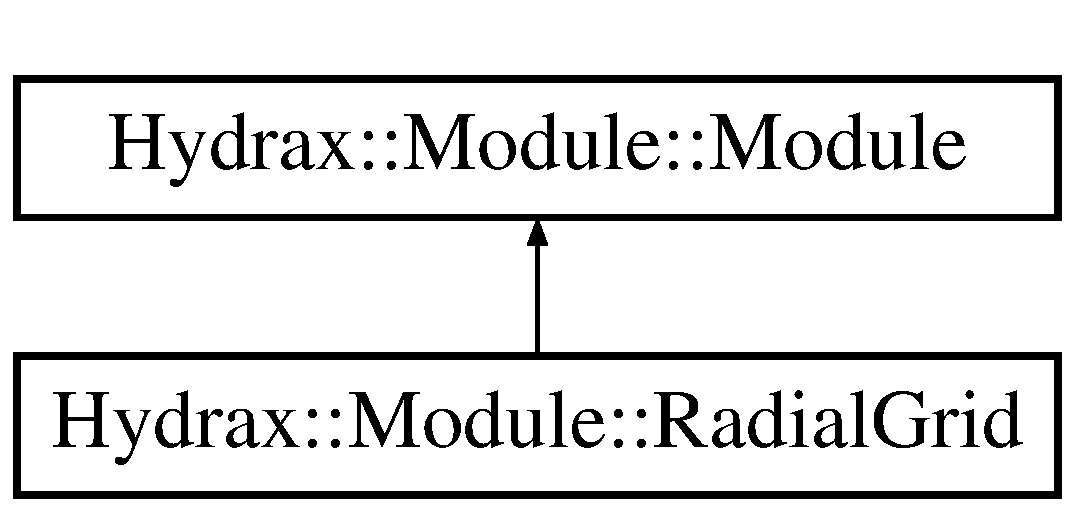
\includegraphics[height=2cm]{class_hydrax_1_1_module_1_1_radial_grid}
\end{center}
\end{figure}
\subsection*{Classes}
\begin{CompactItemize}
\item 
struct \hyperlink{struct_hydrax_1_1_module_1_1_radial_grid_1_1_options}{Options}
\end{CompactItemize}
\subsection*{Public Member Functions}
\begin{CompactItemize}
\item 
\hyperlink{class_hydrax_1_1_module_1_1_radial_grid_5633f577c51302d5175f4feddfa80d19}{RadialGrid} (\hyperlink{class_hydrax_1_1_hydrax}{Hydrax} $\ast$h, \hyperlink{class_hydrax_1_1_noise_1_1_noise}{Noise::Noise} $\ast$n, const \hyperlink{class_hydrax_1_1_material_manager_aa14689cd1c259f48954dfecda9b296f}{MaterialManager::NormalMode} \&NormalMode)
\item 
\hyperlink{class_hydrax_1_1_module_1_1_radial_grid_bc52ff8727a537d5303fabc1179fa45f}{RadialGrid} (\hyperlink{class_hydrax_1_1_hydrax}{Hydrax} $\ast$h, \hyperlink{class_hydrax_1_1_noise_1_1_noise}{Noise::Noise} $\ast$n, const \hyperlink{class_hydrax_1_1_material_manager_aa14689cd1c259f48954dfecda9b296f}{MaterialManager::NormalMode} \&NormalMode, const \hyperlink{struct_hydrax_1_1_module_1_1_radial_grid_1_1_options}{Options} \&\hyperlink{struct_hydrax_1_1_module_1_1_radial_grid_1_1_options}{Options})
\item 
\hyperlink{class_hydrax_1_1_module_1_1_radial_grid_f8caf3997cfc178019db4ac735394b7c}{$\sim$RadialGrid} ()
\item 
void \hyperlink{class_hydrax_1_1_module_1_1_radial_grid_8c0f059e53170e7d1114bb7faecbcb0a}{create} ()
\item 
void \hyperlink{class_hydrax_1_1_module_1_1_radial_grid_5b595aede4b235740be75fb5cf1072cf}{remove} ()
\item 
void \hyperlink{class_hydrax_1_1_module_1_1_radial_grid_ee5199bfbee4429ab428d477e36443dd}{update} (const Ogre::Real \&timeSinceLastFrame)
\item 
void \hyperlink{class_hydrax_1_1_module_1_1_radial_grid_cfc2ae157df9b6159302a90561ffc038}{setOptions} (const \hyperlink{struct_hydrax_1_1_module_1_1_radial_grid_1_1_options}{Options} \&\hyperlink{struct_hydrax_1_1_module_1_1_radial_grid_1_1_options}{Options})
\item 
void \hyperlink{class_hydrax_1_1_module_1_1_radial_grid_241237552e8f36f7e4696b8bad7acc91}{saveCfg} (Ogre::String \&Data)
\item 
bool \hyperlink{class_hydrax_1_1_module_1_1_radial_grid_31b3bab8e74f2f1e316a1800470ac685}{loadCfg} (Ogre::ConfigFile \&CfgFile)
\item 
float \hyperlink{class_hydrax_1_1_module_1_1_radial_grid_0289caac51efbaf6a085bbb94eb22c4c}{getHeigth} (const Ogre::Vector2 \&Position)
\item 
const \hyperlink{struct_hydrax_1_1_module_1_1_radial_grid_1_1_options}{Options} \& \hyperlink{class_hydrax_1_1_module_1_1_radial_grid_cf6dab9b665fcf36467219bcabc5aa14}{getOptions} () const 
\item 
const bool \hyperlink{class_hydrax_1_1_module_1_1_radial_grid_8fde866e72e871e7aaf76957236b7b15}{\_\-createGeometry} (\hyperlink{class_hydrax_1_1_mesh}{Mesh} $\ast$mMesh) const 
\end{CompactItemize}


\subsection{Detailed Description}
\hyperlink{class_hydrax_1_1_hydrax}{Hydrax} radial grid module 

\subsection{Constructor \& Destructor Documentation}
\hypertarget{class_hydrax_1_1_module_1_1_radial_grid_5633f577c51302d5175f4feddfa80d19}{
\index{Hydrax::Module::RadialGrid@{Hydrax::Module::RadialGrid}!RadialGrid@{RadialGrid}}
\index{RadialGrid@{RadialGrid}!Hydrax::Module::RadialGrid@{Hydrax::Module::RadialGrid}}
\subsubsection[{RadialGrid}]{\setlength{\rightskip}{0pt plus 5cm}Hydrax::Module::RadialGrid::RadialGrid ({\bf Hydrax} $\ast$ {\em h}, \/  {\bf Noise::Noise} $\ast$ {\em n}, \/  const {\bf MaterialManager::NormalMode} \& {\em NormalMode})}}
\label{class_hydrax_1_1_module_1_1_radial_grid_5633f577c51302d5175f4feddfa80d19}


Constructor \begin{Desc}
\item[Parameters:]
\begin{description}
\item[{\em h}]\hyperlink{class_hydrax_1_1_hydrax}{Hydrax} manager pointer \item[{\em n}]\hyperlink{class_hydrax_1_1_hydrax}{Hydrax} noise module \item[{\em NormalMode}]Switch between \hyperlink{class_hydrax_1_1_material_manager_aa14689cd1c259f48954dfecda9b296ffe4d6257f673cf503a9905fb2576288f}{MaterialManager::NM\_\-VERTEX} and Materialmanager::NM\_\-RTT \end{description}
\end{Desc}
\hypertarget{class_hydrax_1_1_module_1_1_radial_grid_bc52ff8727a537d5303fabc1179fa45f}{
\index{Hydrax::Module::RadialGrid@{Hydrax::Module::RadialGrid}!RadialGrid@{RadialGrid}}
\index{RadialGrid@{RadialGrid}!Hydrax::Module::RadialGrid@{Hydrax::Module::RadialGrid}}
\subsubsection[{RadialGrid}]{\setlength{\rightskip}{0pt plus 5cm}Hydrax::Module::RadialGrid::RadialGrid ({\bf Hydrax} $\ast$ {\em h}, \/  {\bf Noise::Noise} $\ast$ {\em n}, \/  const {\bf MaterialManager::NormalMode} \& {\em NormalMode}, \/  const {\bf Options} \& {\em Options})}}
\label{class_hydrax_1_1_module_1_1_radial_grid_bc52ff8727a537d5303fabc1179fa45f}


Constructor \begin{Desc}
\item[Parameters:]
\begin{description}
\item[{\em h}]\hyperlink{class_hydrax_1_1_hydrax}{Hydrax} manager pointer \item[{\em n}]\hyperlink{class_hydrax_1_1_hydrax}{Hydrax} noise module \item[{\em NormalMode}]Switch between \hyperlink{class_hydrax_1_1_material_manager_aa14689cd1c259f48954dfecda9b296ffe4d6257f673cf503a9905fb2576288f}{MaterialManager::NM\_\-VERTEX} and Materialmanager::NM\_\-RTT \item[{\em \hyperlink{struct_hydrax_1_1_module_1_1_radial_grid_1_1_options}{Options}}]Perlin options \end{description}
\end{Desc}
\hypertarget{class_hydrax_1_1_module_1_1_radial_grid_f8caf3997cfc178019db4ac735394b7c}{
\index{Hydrax::Module::RadialGrid@{Hydrax::Module::RadialGrid}!$\sim$RadialGrid@{$\sim$RadialGrid}}
\index{$\sim$RadialGrid@{$\sim$RadialGrid}!Hydrax::Module::RadialGrid@{Hydrax::Module::RadialGrid}}
\subsubsection[{$\sim$RadialGrid}]{\setlength{\rightskip}{0pt plus 5cm}Hydrax::Module::RadialGrid::$\sim$RadialGrid ()}}
\label{class_hydrax_1_1_module_1_1_radial_grid_f8caf3997cfc178019db4ac735394b7c}


Destructor 

\subsection{Member Function Documentation}
\hypertarget{class_hydrax_1_1_module_1_1_radial_grid_8fde866e72e871e7aaf76957236b7b15}{
\index{Hydrax::Module::RadialGrid@{Hydrax::Module::RadialGrid}!\_\-createGeometry@{\_\-createGeometry}}
\index{\_\-createGeometry@{\_\-createGeometry}!Hydrax::Module::RadialGrid@{Hydrax::Module::RadialGrid}}
\subsubsection[{\_\-createGeometry}]{\setlength{\rightskip}{0pt plus 5cm}const bool Hydrax::Module::RadialGrid::\_\-createGeometry ({\bf Mesh} $\ast$ {\em mMesh}) const\hspace{0.3cm}{\tt  \mbox{[}virtual\mbox{]}}}}
\label{class_hydrax_1_1_module_1_1_radial_grid_8fde866e72e871e7aaf76957236b7b15}


Create geometry in module(If special geometry is needed) \begin{Desc}
\item[Parameters:]
\begin{description}
\item[{\em mMesh}]\hyperlink{class_hydrax_1_1_mesh}{Mesh} \end{description}
\end{Desc}
\begin{Desc}
\item[Returns:]false if it must be create by default Mesh::\_\-createGeometry() fnc. \end{Desc}


Reimplemented from \hyperlink{class_hydrax_1_1_module_1_1_module_e58d6103f780287cb00a8c4647db667e}{Hydrax::Module::Module}.\hypertarget{class_hydrax_1_1_module_1_1_radial_grid_8c0f059e53170e7d1114bb7faecbcb0a}{
\index{Hydrax::Module::RadialGrid@{Hydrax::Module::RadialGrid}!create@{create}}
\index{create@{create}!Hydrax::Module::RadialGrid@{Hydrax::Module::RadialGrid}}
\subsubsection[{create}]{\setlength{\rightskip}{0pt plus 5cm}void Hydrax::Module::RadialGrid::create ()\hspace{0.3cm}{\tt  \mbox{[}virtual\mbox{]}}}}
\label{class_hydrax_1_1_module_1_1_radial_grid_8c0f059e53170e7d1114bb7faecbcb0a}


Create 

Reimplemented from \hyperlink{class_hydrax_1_1_module_1_1_module_4b696328c3fc1496f757e929f44f3258}{Hydrax::Module::Module}.\hypertarget{class_hydrax_1_1_module_1_1_radial_grid_0289caac51efbaf6a085bbb94eb22c4c}{
\index{Hydrax::Module::RadialGrid@{Hydrax::Module::RadialGrid}!getHeigth@{getHeigth}}
\index{getHeigth@{getHeigth}!Hydrax::Module::RadialGrid@{Hydrax::Module::RadialGrid}}
\subsubsection[{getHeigth}]{\setlength{\rightskip}{0pt plus 5cm}float Hydrax::Module::RadialGrid::getHeigth (const Ogre::Vector2 \& {\em Position})\hspace{0.3cm}{\tt  \mbox{[}virtual\mbox{]}}}}
\label{class_hydrax_1_1_module_1_1_radial_grid_0289caac51efbaf6a085bbb94eb22c4c}


Get the current heigth at a especified world-space point \begin{Desc}
\item[Parameters:]
\begin{description}
\item[{\em Position}]X/Z World position \end{description}
\end{Desc}
\begin{Desc}
\item[Returns:]Heigth at the given position in y-World coordinates, if it's outside of the water return -1 \end{Desc}


Reimplemented from \hyperlink{class_hydrax_1_1_module_1_1_module_c61f89589d3b1bc7256731ddb7af7d0b}{Hydrax::Module::Module}.\hypertarget{class_hydrax_1_1_module_1_1_radial_grid_cf6dab9b665fcf36467219bcabc5aa14}{
\index{Hydrax::Module::RadialGrid@{Hydrax::Module::RadialGrid}!getOptions@{getOptions}}
\index{getOptions@{getOptions}!Hydrax::Module::RadialGrid@{Hydrax::Module::RadialGrid}}
\subsubsection[{getOptions}]{\setlength{\rightskip}{0pt plus 5cm}const {\bf Options}\& Hydrax::Module::RadialGrid::getOptions () const\hspace{0.3cm}{\tt  \mbox{[}inline\mbox{]}}}}
\label{class_hydrax_1_1_module_1_1_radial_grid_cf6dab9b665fcf36467219bcabc5aa14}


Get current options \begin{Desc}
\item[Returns:]Current options \end{Desc}
\hypertarget{class_hydrax_1_1_module_1_1_radial_grid_31b3bab8e74f2f1e316a1800470ac685}{
\index{Hydrax::Module::RadialGrid@{Hydrax::Module::RadialGrid}!loadCfg@{loadCfg}}
\index{loadCfg@{loadCfg}!Hydrax::Module::RadialGrid@{Hydrax::Module::RadialGrid}}
\subsubsection[{loadCfg}]{\setlength{\rightskip}{0pt plus 5cm}bool Hydrax::Module::RadialGrid::loadCfg (Ogre::ConfigFile \& {\em CfgFile})\hspace{0.3cm}{\tt  \mbox{[}virtual\mbox{]}}}}
\label{class_hydrax_1_1_module_1_1_radial_grid_31b3bab8e74f2f1e316a1800470ac685}


Load config \begin{Desc}
\item[Parameters:]
\begin{description}
\item[{\em CgfFile}]Ogre::ConfigFile reference \end{description}
\end{Desc}
\begin{Desc}
\item[Returns:]True if is the correct module config \end{Desc}


Reimplemented from \hyperlink{class_hydrax_1_1_module_1_1_module_bedb96357608c0744bb7816ae1c2b0bb}{Hydrax::Module::Module}.\hypertarget{class_hydrax_1_1_module_1_1_radial_grid_5b595aede4b235740be75fb5cf1072cf}{
\index{Hydrax::Module::RadialGrid@{Hydrax::Module::RadialGrid}!remove@{remove}}
\index{remove@{remove}!Hydrax::Module::RadialGrid@{Hydrax::Module::RadialGrid}}
\subsubsection[{remove}]{\setlength{\rightskip}{0pt plus 5cm}void Hydrax::Module::RadialGrid::remove ()\hspace{0.3cm}{\tt  \mbox{[}virtual\mbox{]}}}}
\label{class_hydrax_1_1_module_1_1_radial_grid_5b595aede4b235740be75fb5cf1072cf}


Remove 

Reimplemented from \hyperlink{class_hydrax_1_1_module_1_1_module_21f60a53a99d72ff00d3fe5565518165}{Hydrax::Module::Module}.\hypertarget{class_hydrax_1_1_module_1_1_radial_grid_241237552e8f36f7e4696b8bad7acc91}{
\index{Hydrax::Module::RadialGrid@{Hydrax::Module::RadialGrid}!saveCfg@{saveCfg}}
\index{saveCfg@{saveCfg}!Hydrax::Module::RadialGrid@{Hydrax::Module::RadialGrid}}
\subsubsection[{saveCfg}]{\setlength{\rightskip}{0pt plus 5cm}void Hydrax::Module::RadialGrid::saveCfg (Ogre::String \& {\em Data})\hspace{0.3cm}{\tt  \mbox{[}virtual\mbox{]}}}}
\label{class_hydrax_1_1_module_1_1_radial_grid_241237552e8f36f7e4696b8bad7acc91}


Save config \begin{Desc}
\item[Parameters:]
\begin{description}
\item[{\em Data}]String reference \end{description}
\end{Desc}


Reimplemented from \hyperlink{class_hydrax_1_1_module_1_1_module_998a5baf42f57b02ca7bc20bc12f95a9}{Hydrax::Module::Module}.\hypertarget{class_hydrax_1_1_module_1_1_radial_grid_cfc2ae157df9b6159302a90561ffc038}{
\index{Hydrax::Module::RadialGrid@{Hydrax::Module::RadialGrid}!setOptions@{setOptions}}
\index{setOptions@{setOptions}!Hydrax::Module::RadialGrid@{Hydrax::Module::RadialGrid}}
\subsubsection[{setOptions}]{\setlength{\rightskip}{0pt plus 5cm}void Hydrax::Module::RadialGrid::setOptions (const {\bf Options} \& {\em Options})}}
\label{class_hydrax_1_1_module_1_1_radial_grid_cfc2ae157df9b6159302a90561ffc038}


Set options \begin{Desc}
\item[Parameters:]
\begin{description}
\item[{\em \hyperlink{struct_hydrax_1_1_module_1_1_radial_grid_1_1_options}{Options}}]\hyperlink{struct_hydrax_1_1_module_1_1_radial_grid_1_1_options}{Options} \end{description}
\end{Desc}
\hypertarget{class_hydrax_1_1_module_1_1_radial_grid_ee5199bfbee4429ab428d477e36443dd}{
\index{Hydrax::Module::RadialGrid@{Hydrax::Module::RadialGrid}!update@{update}}
\index{update@{update}!Hydrax::Module::RadialGrid@{Hydrax::Module::RadialGrid}}
\subsubsection[{update}]{\setlength{\rightskip}{0pt plus 5cm}void Hydrax::Module::RadialGrid::update (const Ogre::Real \& {\em timeSinceLastFrame})\hspace{0.3cm}{\tt  \mbox{[}virtual\mbox{]}}}}
\label{class_hydrax_1_1_module_1_1_radial_grid_ee5199bfbee4429ab428d477e36443dd}


Call it each frame \begin{Desc}
\item[Parameters:]
\begin{description}
\item[{\em timeSinceLastFrame}]Time since last frame(delta) \end{description}
\end{Desc}


Reimplemented from \hyperlink{class_hydrax_1_1_module_1_1_module_2042d450f99d9348fa4b7bd29ba89df3}{Hydrax::Module::Module}.

The documentation for this class was generated from the following files:\begin{CompactItemize}
\item 
C:/Hydrax/v0.5.1/Hydrax/src/Hydrax/Modules/RadialGrid/\hyperlink{_radial_grid_8h}{RadialGrid.h}\item 
C:/Hydrax/v0.5.1/Hydrax/src/Hydrax/Modules/RadialGrid/\hyperlink{_radial_grid_8cpp}{RadialGrid.cpp}\end{CompactItemize}

\hypertarget{struct_hydrax_1_1_module_1_1_radial_grid_1_1_options}{
\section{Hydrax::Module::RadialGrid::RadialGrid::Options Struct Reference}
\label{struct_hydrax_1_1_module_1_1_radial_grid_1_1_options}\index{Hydrax::Module::RadialGrid::Options@{Hydrax::Module::RadialGrid::Options}}
}
{\tt \#include $<$RadialGrid.h$>$}

\subsection*{Public Member Functions}
\begin{CompactItemize}
\item 
\hyperlink{struct_hydrax_1_1_module_1_1_radial_grid_1_1_options_124d0f633f807b2cd7e8f4409a76fbc4}{Options} ()
\item 
\hyperlink{struct_hydrax_1_1_module_1_1_radial_grid_1_1_options_574fc5fbf5d20a1fbc5af03fea97bbca}{Options} (const int \&\_\-Steps, const int \&\_\-Circles, const float \&\_\-Radius)
\item 
\hyperlink{struct_hydrax_1_1_module_1_1_radial_grid_1_1_options_e270a3ae95902e237814a32a64a916c5}{Options} (const int \&\_\-Steps, const int \&\_\-Circles, const float \&\_\-Radius, const bool \&\_\-Smooth, const bool \&\_\-ChoppyWaves, const float \&\_\-ChoppyStrength, const float \&\_\-StepSizeCube, const float \&\_\-StepSizeFive, const float \&\_\-StepSizeLin, const float \&\_\-Strength)
\end{CompactItemize}
\subsection*{Public Attributes}
\begin{CompactItemize}
\item 
int \hyperlink{struct_hydrax_1_1_module_1_1_radial_grid_1_1_options_902da4f0f8dfa6f9e47e48a7af346e2b}{Steps}
\begin{CompactList}\small\item\em Number of steps (Per circle). \item\end{CompactList}\item 
int \hyperlink{struct_hydrax_1_1_module_1_1_radial_grid_1_1_options_efe98acc6ec2bfcbd0776ec43343819e}{Circles}
\begin{CompactList}\small\item\em Number of circles. \item\end{CompactList}\item 
float \hyperlink{struct_hydrax_1_1_module_1_1_radial_grid_1_1_options_2ebdfa6131bc283e2cc3ec8d74a3d712}{Radius}
\begin{CompactList}\small\item\em Radius (In world units). \item\end{CompactList}\item 
bool \hyperlink{struct_hydrax_1_1_module_1_1_radial_grid_1_1_options_1004e40adf66a0c305bb6cb4ca46d4a6}{Smooth}
\begin{CompactList}\small\item\em Smooth. \item\end{CompactList}\item 
bool \hyperlink{struct_hydrax_1_1_module_1_1_radial_grid_1_1_options_8f2d48d2bc30eaa1862696aadacd9241}{ChoppyWaves}
\begin{CompactList}\small\item\em Choppy waves. \item\end{CompactList}\item 
float \hyperlink{struct_hydrax_1_1_module_1_1_radial_grid_1_1_options_bc3d5ce9e689f4ae7eacf517c25a7c78}{ChoppyStrength}
\begin{CompactList}\small\item\em Choppy waves strength. \item\end{CompactList}\item 
float \hyperlink{struct_hydrax_1_1_module_1_1_radial_grid_1_1_options_e405499a76f4c1805c559901fbdad2cd}{StepSizeCube}
\begin{CompactList}\small\item\em Step cube size. \item\end{CompactList}\item 
float \hyperlink{struct_hydrax_1_1_module_1_1_radial_grid_1_1_options_fb39f5d35557b182254e6685251b17df}{StepSizeFive}
\begin{CompactList}\small\item\em Step size five. \item\end{CompactList}\item 
float \hyperlink{struct_hydrax_1_1_module_1_1_radial_grid_1_1_options_933a688b6f7230ad6ff130298edbb795}{StepSizeLin}
\begin{CompactList}\small\item\em Step lin size. \item\end{CompactList}\item 
float \hyperlink{struct_hydrax_1_1_module_1_1_radial_grid_1_1_options_8f11d4879ffadedf6c1ba0519e0bbbfc}{Strength}
\begin{CompactList}\small\item\em Water strength. \item\end{CompactList}\end{CompactItemize}


\subsection{Detailed Description}
Struct wich contains \hyperlink{class_hydrax_1_1_hydrax}{Hydrax} simple grid module options 

\subsection{Constructor \& Destructor Documentation}
\hypertarget{struct_hydrax_1_1_module_1_1_radial_grid_1_1_options_124d0f633f807b2cd7e8f4409a76fbc4}{
\index{Hydrax::Module::RadialGrid::Options@{Hydrax::Module::RadialGrid::Options}!Options@{Options}}
\index{Options@{Options}!Hydrax::Module::RadialGrid::Options@{Hydrax::Module::RadialGrid::Options}}
\subsubsection[{Options}]{\setlength{\rightskip}{0pt plus 5cm}Hydrax::Module::RadialGrid::RadialGrid::Options::Options ()\hspace{0.3cm}{\tt  \mbox{[}inline\mbox{]}}}}
\label{struct_hydrax_1_1_module_1_1_radial_grid_1_1_options_124d0f633f807b2cd7e8f4409a76fbc4}


Default constructor \hypertarget{struct_hydrax_1_1_module_1_1_radial_grid_1_1_options_574fc5fbf5d20a1fbc5af03fea97bbca}{
\index{Hydrax::Module::RadialGrid::Options@{Hydrax::Module::RadialGrid::Options}!Options@{Options}}
\index{Options@{Options}!Hydrax::Module::RadialGrid::Options@{Hydrax::Module::RadialGrid::Options}}
\subsubsection[{Options}]{\setlength{\rightskip}{0pt plus 5cm}Hydrax::Module::RadialGrid::RadialGrid::Options::Options (const int \& {\em \_\-Steps}, \/  const int \& {\em \_\-Circles}, \/  const float \& {\em \_\-Radius})\hspace{0.3cm}{\tt  \mbox{[}inline\mbox{]}}}}
\label{struct_hydrax_1_1_module_1_1_radial_grid_1_1_options_574fc5fbf5d20a1fbc5af03fea97bbca}


Constructor \begin{Desc}
\item[Parameters:]
\begin{description}
\item[{\em \_\-Steps}]Number of steps per circle \item[{\em \_\-Circles}]Number of circles \item[{\em \_\-Radius}]\hyperlink{class_hydrax_1_1_mesh}{Mesh} radius \end{description}
\end{Desc}
\hypertarget{struct_hydrax_1_1_module_1_1_radial_grid_1_1_options_e270a3ae95902e237814a32a64a916c5}{
\index{Hydrax::Module::RadialGrid::Options@{Hydrax::Module::RadialGrid::Options}!Options@{Options}}
\index{Options@{Options}!Hydrax::Module::RadialGrid::Options@{Hydrax::Module::RadialGrid::Options}}
\subsubsection[{Options}]{\setlength{\rightskip}{0pt plus 5cm}Hydrax::Module::RadialGrid::RadialGrid::Options::Options (const int \& {\em \_\-Steps}, \/  const int \& {\em \_\-Circles}, \/  const float \& {\em \_\-Radius}, \/  const bool \& {\em \_\-Smooth}, \/  const bool \& {\em \_\-ChoppyWaves}, \/  const float \& {\em \_\-ChoppyStrength}, \/  const float \& {\em \_\-StepSizeCube}, \/  const float \& {\em \_\-StepSizeFive}, \/  const float \& {\em \_\-StepSizeLin}, \/  const float \& {\em \_\-Strength})\hspace{0.3cm}{\tt  \mbox{[}inline\mbox{]}}}}
\label{struct_hydrax_1_1_module_1_1_radial_grid_1_1_options_e270a3ae95902e237814a32a64a916c5}


Constructor \begin{Desc}
\item[Parameters:]
\begin{description}
\item[{\em \_\-Steps}]Number of steps per circle \item[{\em \_\-Circles}]Number of circles \item[{\em \_\-Radius}]\hyperlink{class_hydrax_1_1_mesh}{Mesh} radius \item[{\em \_\-Smooth}]Smooth vertex? \item[{\em \_\-ChoppyWaves}]Choppy waves enabled? Note: Only with Materialmanager::NM\_\-VERTEX normal mode. \item[{\em \_\-ChoppyStrength}]Choppy waves strength Note: Only with Materialmanager::NM\_\-VERTEX normal mode. \item[{\em \_\-StepSizeCube}]Step cube size \item[{\em \_\-StepSizeFive}]Step five size \item[{\em \_\-StepSizeLin}]Step lin size \item[{\em \_\-Strength}]Water strength \end{description}
\end{Desc}


\subsection{Member Data Documentation}
\hypertarget{struct_hydrax_1_1_module_1_1_radial_grid_1_1_options_bc3d5ce9e689f4ae7eacf517c25a7c78}{
\index{Hydrax::Module::RadialGrid::Options@{Hydrax::Module::RadialGrid::Options}!ChoppyStrength@{ChoppyStrength}}
\index{ChoppyStrength@{ChoppyStrength}!Hydrax::Module::RadialGrid::Options@{Hydrax::Module::RadialGrid::Options}}
\subsubsection[{ChoppyStrength}]{\setlength{\rightskip}{0pt plus 5cm}float Hydrax::Module::RadialGrid::RadialGrid::Options::ChoppyStrength}}
\label{struct_hydrax_1_1_module_1_1_radial_grid_1_1_options_bc3d5ce9e689f4ae7eacf517c25a7c78}


Choppy waves strength. 

\hypertarget{struct_hydrax_1_1_module_1_1_radial_grid_1_1_options_8f2d48d2bc30eaa1862696aadacd9241}{
\index{Hydrax::Module::RadialGrid::Options@{Hydrax::Module::RadialGrid::Options}!ChoppyWaves@{ChoppyWaves}}
\index{ChoppyWaves@{ChoppyWaves}!Hydrax::Module::RadialGrid::Options@{Hydrax::Module::RadialGrid::Options}}
\subsubsection[{ChoppyWaves}]{\setlength{\rightskip}{0pt plus 5cm}bool Hydrax::Module::RadialGrid::RadialGrid::Options::ChoppyWaves}}
\label{struct_hydrax_1_1_module_1_1_radial_grid_1_1_options_8f2d48d2bc30eaa1862696aadacd9241}


Choppy waves. 

\hypertarget{struct_hydrax_1_1_module_1_1_radial_grid_1_1_options_efe98acc6ec2bfcbd0776ec43343819e}{
\index{Hydrax::Module::RadialGrid::Options@{Hydrax::Module::RadialGrid::Options}!Circles@{Circles}}
\index{Circles@{Circles}!Hydrax::Module::RadialGrid::Options@{Hydrax::Module::RadialGrid::Options}}
\subsubsection[{Circles}]{\setlength{\rightskip}{0pt plus 5cm}int Hydrax::Module::RadialGrid::RadialGrid::Options::Circles}}
\label{struct_hydrax_1_1_module_1_1_radial_grid_1_1_options_efe98acc6ec2bfcbd0776ec43343819e}


Number of circles. 

\hypertarget{struct_hydrax_1_1_module_1_1_radial_grid_1_1_options_2ebdfa6131bc283e2cc3ec8d74a3d712}{
\index{Hydrax::Module::RadialGrid::Options@{Hydrax::Module::RadialGrid::Options}!Radius@{Radius}}
\index{Radius@{Radius}!Hydrax::Module::RadialGrid::Options@{Hydrax::Module::RadialGrid::Options}}
\subsubsection[{Radius}]{\setlength{\rightskip}{0pt plus 5cm}float Hydrax::Module::RadialGrid::RadialGrid::Options::Radius}}
\label{struct_hydrax_1_1_module_1_1_radial_grid_1_1_options_2ebdfa6131bc283e2cc3ec8d74a3d712}


Radius (In world units). 

\hypertarget{struct_hydrax_1_1_module_1_1_radial_grid_1_1_options_1004e40adf66a0c305bb6cb4ca46d4a6}{
\index{Hydrax::Module::RadialGrid::Options@{Hydrax::Module::RadialGrid::Options}!Smooth@{Smooth}}
\index{Smooth@{Smooth}!Hydrax::Module::RadialGrid::Options@{Hydrax::Module::RadialGrid::Options}}
\subsubsection[{Smooth}]{\setlength{\rightskip}{0pt plus 5cm}bool Hydrax::Module::RadialGrid::RadialGrid::Options::Smooth}}
\label{struct_hydrax_1_1_module_1_1_radial_grid_1_1_options_1004e40adf66a0c305bb6cb4ca46d4a6}


Smooth. 

\hypertarget{struct_hydrax_1_1_module_1_1_radial_grid_1_1_options_902da4f0f8dfa6f9e47e48a7af346e2b}{
\index{Hydrax::Module::RadialGrid::Options@{Hydrax::Module::RadialGrid::Options}!Steps@{Steps}}
\index{Steps@{Steps}!Hydrax::Module::RadialGrid::Options@{Hydrax::Module::RadialGrid::Options}}
\subsubsection[{Steps}]{\setlength{\rightskip}{0pt plus 5cm}int Hydrax::Module::RadialGrid::RadialGrid::Options::Steps}}
\label{struct_hydrax_1_1_module_1_1_radial_grid_1_1_options_902da4f0f8dfa6f9e47e48a7af346e2b}


Number of steps (Per circle). 

\hypertarget{struct_hydrax_1_1_module_1_1_radial_grid_1_1_options_e405499a76f4c1805c559901fbdad2cd}{
\index{Hydrax::Module::RadialGrid::Options@{Hydrax::Module::RadialGrid::Options}!StepSizeCube@{StepSizeCube}}
\index{StepSizeCube@{StepSizeCube}!Hydrax::Module::RadialGrid::Options@{Hydrax::Module::RadialGrid::Options}}
\subsubsection[{StepSizeCube}]{\setlength{\rightskip}{0pt plus 5cm}float Hydrax::Module::RadialGrid::RadialGrid::Options::StepSizeCube}}
\label{struct_hydrax_1_1_module_1_1_radial_grid_1_1_options_e405499a76f4c1805c559901fbdad2cd}


Step cube size. 

\hypertarget{struct_hydrax_1_1_module_1_1_radial_grid_1_1_options_fb39f5d35557b182254e6685251b17df}{
\index{Hydrax::Module::RadialGrid::Options@{Hydrax::Module::RadialGrid::Options}!StepSizeFive@{StepSizeFive}}
\index{StepSizeFive@{StepSizeFive}!Hydrax::Module::RadialGrid::Options@{Hydrax::Module::RadialGrid::Options}}
\subsubsection[{StepSizeFive}]{\setlength{\rightskip}{0pt plus 5cm}float Hydrax::Module::RadialGrid::RadialGrid::Options::StepSizeFive}}
\label{struct_hydrax_1_1_module_1_1_radial_grid_1_1_options_fb39f5d35557b182254e6685251b17df}


Step size five. 

\hypertarget{struct_hydrax_1_1_module_1_1_radial_grid_1_1_options_933a688b6f7230ad6ff130298edbb795}{
\index{Hydrax::Module::RadialGrid::Options@{Hydrax::Module::RadialGrid::Options}!StepSizeLin@{StepSizeLin}}
\index{StepSizeLin@{StepSizeLin}!Hydrax::Module::RadialGrid::Options@{Hydrax::Module::RadialGrid::Options}}
\subsubsection[{StepSizeLin}]{\setlength{\rightskip}{0pt plus 5cm}float Hydrax::Module::RadialGrid::RadialGrid::Options::StepSizeLin}}
\label{struct_hydrax_1_1_module_1_1_radial_grid_1_1_options_933a688b6f7230ad6ff130298edbb795}


Step lin size. 

\hypertarget{struct_hydrax_1_1_module_1_1_radial_grid_1_1_options_8f11d4879ffadedf6c1ba0519e0bbbfc}{
\index{Hydrax::Module::RadialGrid::Options@{Hydrax::Module::RadialGrid::Options}!Strength@{Strength}}
\index{Strength@{Strength}!Hydrax::Module::RadialGrid::Options@{Hydrax::Module::RadialGrid::Options}}
\subsubsection[{Strength}]{\setlength{\rightskip}{0pt plus 5cm}float Hydrax::Module::RadialGrid::RadialGrid::Options::Strength}}
\label{struct_hydrax_1_1_module_1_1_radial_grid_1_1_options_8f11d4879ffadedf6c1ba0519e0bbbfc}


Water strength. 



The documentation for this struct was generated from the following file:\begin{CompactItemize}
\item 
C:/Hydrax/v0.5.1/Hydrax/src/Hydrax/Modules/RadialGrid/\hyperlink{_radial_grid_8h}{RadialGrid.h}\end{CompactItemize}

\hypertarget{class_hydrax_1_1_rtt_manager}{
\section{Hydrax::RttManager Class Reference}
\label{class_hydrax_1_1_rtt_manager}\index{Hydrax::RttManager@{Hydrax::RttManager}}
}
{\tt \#include $<$RttManager.h$>$}

\subsection*{Classes}
\begin{CompactItemize}
\item 
class \textbf{CDepthListener}
\item 
class \textbf{CDepthReflectionListener}
\item 
class \textbf{CGPUNormalMapListener}
\item 
class \textbf{CReflectionListener}
\item 
class \textbf{CRefractionListener}
\item 
class \hyperlink{class_hydrax_1_1_rtt_manager_1_1_rtt_listener}{RttListener}
\item 
struct \hyperlink{struct_hydrax_1_1_rtt_manager_1_1_rtt_options}{RttOptions}
\end{CompactItemize}
\subsection*{Public Types}
\begin{CompactItemize}
\item 
enum \hyperlink{class_hydrax_1_1_rtt_manager_9753d012b355eba64cff2b19bb6f76ed}{RttType} \{ \par
\hyperlink{class_hydrax_1_1_rtt_manager_9753d012b355eba64cff2b19bb6f76ed46bf97fd6dfb5127e198ba5864d177cf}{RTT\_\-REFLECTION} =  0, 
\hyperlink{class_hydrax_1_1_rtt_manager_9753d012b355eba64cff2b19bb6f76ed19faf1e23955005ac93e096fb9c7745a}{RTT\_\-REFRACTION} =  1, 
\hyperlink{class_hydrax_1_1_rtt_manager_9753d012b355eba64cff2b19bb6f76ed8a220f3d2252dd891f89d11242f9d0f6}{RTT\_\-DEPTH} =  2, 
\hyperlink{class_hydrax_1_1_rtt_manager_9753d012b355eba64cff2b19bb6f76ed307732729f853596d0e8015b707ccea7}{RTT\_\-DEPTH\_\-REFLECTION} =  3, 
\par
\hyperlink{class_hydrax_1_1_rtt_manager_9753d012b355eba64cff2b19bb6f76ed4d2aa8377c7593dcb15b656f4eb1bf1b}{RTT\_\-DEPTH\_\-AIP} =  4, 
\hyperlink{class_hydrax_1_1_rtt_manager_9753d012b355eba64cff2b19bb6f76ede6e0cfde4b1fec5edfc11becf329f9b1}{RTT\_\-GPU\_\-NORMAL\_\-MAP} =  5
 \}
\item 
enum \hyperlink{class_hydrax_1_1_rtt_manager_ab09efbd8ec25f88656a27d6a4f0446e}{BitsPerChannel} \{ \hyperlink{class_hydrax_1_1_rtt_manager_ab09efbd8ec25f88656a27d6a4f0446ecef13aa48bb44d2dddfce5f2705246de}{BPC\_\-8} =  8, 
\hyperlink{class_hydrax_1_1_rtt_manager_ab09efbd8ec25f88656a27d6a4f0446ec40c0b76eaa0f93d42f8ad5835f2e6df}{BPC\_\-16} =  16, 
\hyperlink{class_hydrax_1_1_rtt_manager_ab09efbd8ec25f88656a27d6a4f0446edcc7a5caa6ce6602c0029e67e7ff8b52}{BPC\_\-32} =  32
 \}
\item 
enum \hyperlink{class_hydrax_1_1_rtt_manager_8f74f31025f23f6ed8930a0d79a70731}{NumberOfChannels} \{ \hyperlink{class_hydrax_1_1_rtt_manager_8f74f31025f23f6ed8930a0d79a70731853812ba55b1b6e4ff7a6dc363851d37}{NOC\_\-1} =  1, 
\hyperlink{class_hydrax_1_1_rtt_manager_8f74f31025f23f6ed8930a0d79a707312db56c36f66ea12cbdc86c16c9239847}{NOC\_\-2} =  2, 
\hyperlink{class_hydrax_1_1_rtt_manager_8f74f31025f23f6ed8930a0d79a70731d61a5de75944638e15e54f0c87d4d40c}{NOC\_\-3} =  3, 
\hyperlink{class_hydrax_1_1_rtt_manager_8f74f31025f23f6ed8930a0d79a7073173ec4033a84d7e46c6bddc956dc1a27f}{NOC\_\-4} =  4
 \}
\subsection*{Public Member Functions}
\begin{CompactItemize}
\item 
\hyperlink{class_hydrax_1_1_rtt_manager_5e3cb1cebd7adf7bf69b7b15e120db71}{RttManager} (\hyperlink{class_hydrax_1_1_hydrax}{Hydrax} $\ast$h)
\item 
\hyperlink{class_hydrax_1_1_rtt_manager_bbce4b6993d9362d11366ba11fbee326}{$\sim$RttManager} ()
\item 
void \hyperlink{class_hydrax_1_1_rtt_manager_774efa00a79ade65e726ed0774d2ac2e}{initialize} (const \hyperlink{class_hydrax_1_1_rtt_manager_9753d012b355eba64cff2b19bb6f76ed}{RttType} \&Rtt)
\item 
void \hyperlink{class_hydrax_1_1_rtt_manager_360139ed63706da8ca9ec04716d65574}{remove} (const \hyperlink{class_hydrax_1_1_rtt_manager_9753d012b355eba64cff2b19bb6f76ed}{RttType} \&Rtt)
\item 
void \hyperlink{class_hydrax_1_1_rtt_manager_ed71ea727ed3c835d655437d1c6de232}{removeAll} ()
\item 
const Ogre::String \& \hyperlink{class_hydrax_1_1_rtt_manager_dc5af0a29c8e491e8ea9fba6349e208c}{getRttName} (\hyperlink{class_hydrax_1_1_rtt_manager_9753d012b355eba64cff2b19bb6f76ed}{RttType} Rtt) const 
\item 
Ogre::TexturePtr \hyperlink{class_hydrax_1_1_rtt_manager_4e672cd4cf5361c48e75b559f841602c}{getTexture} (\hyperlink{class_hydrax_1_1_rtt_manager_9753d012b355eba64cff2b19bb6f76ed}{RttType} Rtt)
\item 
Ogre::SceneNode $\ast$ \hyperlink{class_hydrax_1_1_rtt_manager_2c97d4371d854526fb5ffdc37a40a595}{getPlanesSceneNode} ()
\item 
Ogre::MovablePlane $\ast$ \hyperlink{class_hydrax_1_1_rtt_manager_884250dca579c9cdff85bdec278715fe}{getPlane} (\hyperlink{class_hydrax_1_1_rtt_manager_9753d012b355eba64cff2b19bb6f76ed}{RttType} Rtt)
\item 
const \hyperlink{struct_hydrax_1_1_size}{Size} \& \hyperlink{class_hydrax_1_1_rtt_manager_ceb8b7c524ce0e35e493771dab50b4c9}{getTextureSize} (const \hyperlink{class_hydrax_1_1_rtt_manager_9753d012b355eba64cff2b19bb6f76ed}{RttType} \&Rtt) const 
\item 
void \hyperlink{class_hydrax_1_1_rtt_manager_bf7d8e05771b9f904efa09fe94ab0907}{setTextureSize} (const \hyperlink{class_hydrax_1_1_rtt_manager_9753d012b355eba64cff2b19bb6f76ed}{RttType} \&Rtt, const \hyperlink{struct_hydrax_1_1_size}{Size} \&S)
\item 
void \hyperlink{class_hydrax_1_1_rtt_manager_d54dd87efa7baa4a5037faa2e5241738}{setTexturesSize} (const \hyperlink{struct_hydrax_1_1_size}{Size} \&S)
\item 
const Ogre::PixelFormat \hyperlink{class_hydrax_1_1_rtt_manager_e94c4a88b240d9b7be93aa6c1430d2b6}{getPixelFormat} (const \hyperlink{class_hydrax_1_1_rtt_manager_9753d012b355eba64cff2b19bb6f76ed}{RttType} \&Rtt) const 
\item 
void \hyperlink{class_hydrax_1_1_rtt_manager_009e9c7631dad8d588790401cab753b6}{setNumberOfChannels} (const \hyperlink{class_hydrax_1_1_rtt_manager_9753d012b355eba64cff2b19bb6f76ed}{RttType} \&Rtt, const \hyperlink{class_hydrax_1_1_rtt_manager_8f74f31025f23f6ed8930a0d79a70731}{NumberOfChannels} \&NOC)
\item 
const \hyperlink{class_hydrax_1_1_rtt_manager_8f74f31025f23f6ed8930a0d79a70731}{NumberOfChannels} \& \hyperlink{class_hydrax_1_1_rtt_manager_88b7c387e413cf219f399926c2dbea7e}{getNumberOfChannels} (const \hyperlink{class_hydrax_1_1_rtt_manager_9753d012b355eba64cff2b19bb6f76ed}{RttType} \&Rtt) const 
\item 
void \hyperlink{class_hydrax_1_1_rtt_manager_fe968a7c8f23a6fa9b0d5b499ef09491}{setBitsPerChannel} (const \hyperlink{class_hydrax_1_1_rtt_manager_9753d012b355eba64cff2b19bb6f76ed}{RttType} \&Rtt, const \hyperlink{class_hydrax_1_1_rtt_manager_ab09efbd8ec25f88656a27d6a4f0446e}{BitsPerChannel} \&BPC)
\item 
const \hyperlink{class_hydrax_1_1_rtt_manager_ab09efbd8ec25f88656a27d6a4f0446e}{BitsPerChannel} \& \hyperlink{class_hydrax_1_1_rtt_manager_a0834735c92a9f72f34eaee8e6478343}{getBitsPerChannel} (const \hyperlink{class_hydrax_1_1_rtt_manager_9753d012b355eba64cff2b19bb6f76ed}{RttType} \&Rtt) const 
\item 
const \hyperlink{struct_hydrax_1_1_rtt_manager_1_1_rtt_options}{RttOptions} \& \hyperlink{class_hydrax_1_1_rtt_manager_3d6990b4cbbe6da2e1580b289f5329fd}{getRttOptions} (const \hyperlink{class_hydrax_1_1_rtt_manager_9753d012b355eba64cff2b19bb6f76ed}{RttType} \&Rtt) const 
\item 
void \hyperlink{class_hydrax_1_1_rtt_manager_7b473a60a06df9d943a50939e3b26377}{setReflectionDisplacementError} (const Ogre::Real \&ReflectionDisplacementError)
\item 
const Ogre::Real \& \hyperlink{class_hydrax_1_1_rtt_manager_021cdc044e7f215158dc3747419db037}{getReflectionDisplacementError} () const 
\item 
void \hyperlink{class_hydrax_1_1_rtt_manager_46f7b77221e50359657a4ac2f3a2365c}{setDisableReflectionCustomNearCliplPlaneRenderQueues} (const std::vector$<$ Ogre::RenderQueueGroupID $>$ \&DisableReflectionCustomNearClipPlaneRenderQueues)
\item 
const std::vector$<$ Ogre::RenderQueueGroupID $>$ \& \hyperlink{class_hydrax_1_1_rtt_manager_8f851b42bccd3653458dad169b6fcff9}{getDisableReflectionCustomNearClipPlaneRenderQueues} ()
\item 
void \hyperlink{class_hydrax_1_1_rtt_manager_cd9d1c09314e9ada6f8f646b0b97dc48}{addRttListener} (\hyperlink{class_hydrax_1_1_rtt_manager_1_1_rtt_listener}{RttListener} $\ast$l)
\item 
void \hyperlink{class_hydrax_1_1_rtt_manager_9de0d5171c46f27d34493f85e6a4f8c3}{removeRttListener} (\hyperlink{class_hydrax_1_1_rtt_manager_1_1_rtt_listener}{RttListener} $\ast$l, const bool \&releaseMemory=true)
\item 
void \hyperlink{class_hydrax_1_1_rtt_manager_4aee49693758d34cdd0b613f251e09cc}{removeAllRttListeners} (const bool \&releaseMemory=true)
\end{CompactItemize}


\subsection{Detailed Description}
Rtt's manager class 

\subsection{Member Enumeration Documentation}
\hypertarget{class_hydrax_1_1_rtt_manager_ab09efbd8ec25f88656a27d6a4f0446e}{
\index{Hydrax::RttManager@{Hydrax::RttManager}!BitsPerChannel@{BitsPerChannel}}
\index{BitsPerChannel@{BitsPerChannel}!Hydrax::RttManager@{Hydrax::RttManager}}
\subsubsection[{BitsPerChannel}]{\setlength{\rightskip}{0pt plus 5cm}enum {\bf Hydrax::RttManager::BitsPerChannel}}}
\label{class_hydrax_1_1_rtt_manager_ab09efbd8ec25f88656a27d6a4f0446e}


Bits per channel \begin{Desc}
\item[Enumerator: ]\par
\begin{description}
\index{BPC\_\-8@{BPC\_\-8}!Hydrax::RttManager@{Hydrax::RttManager}}\index{Hydrax::RttManager@{Hydrax::RttManager}!BPC\_\-8@{BPC\_\-8}}\item[{\em 
\hypertarget{class_hydrax_1_1_rtt_manager_ab09efbd8ec25f88656a27d6a4f0446ecef13aa48bb44d2dddfce5f2705246de}{
BPC\_\-8}
\label{class_hydrax_1_1_rtt_manager_ab09efbd8ec25f88656a27d6a4f0446ecef13aa48bb44d2dddfce5f2705246de}
}]\index{BPC\_\-16@{BPC\_\-16}!Hydrax::RttManager@{Hydrax::RttManager}}\index{Hydrax::RttManager@{Hydrax::RttManager}!BPC\_\-16@{BPC\_\-16}}\item[{\em 
\hypertarget{class_hydrax_1_1_rtt_manager_ab09efbd8ec25f88656a27d6a4f0446ec40c0b76eaa0f93d42f8ad5835f2e6df}{
BPC\_\-16}
\label{class_hydrax_1_1_rtt_manager_ab09efbd8ec25f88656a27d6a4f0446ec40c0b76eaa0f93d42f8ad5835f2e6df}
}]\index{BPC\_\-32@{BPC\_\-32}!Hydrax::RttManager@{Hydrax::RttManager}}\index{Hydrax::RttManager@{Hydrax::RttManager}!BPC\_\-32@{BPC\_\-32}}\item[{\em 
\hypertarget{class_hydrax_1_1_rtt_manager_ab09efbd8ec25f88656a27d6a4f0446edcc7a5caa6ce6602c0029e67e7ff8b52}{
BPC\_\-32}
\label{class_hydrax_1_1_rtt_manager_ab09efbd8ec25f88656a27d6a4f0446edcc7a5caa6ce6602c0029e67e7ff8b52}
}]\end{description}
\end{Desc}

\hypertarget{class_hydrax_1_1_rtt_manager_8f74f31025f23f6ed8930a0d79a70731}{
\index{Hydrax::RttManager@{Hydrax::RttManager}!NumberOfChannels@{NumberOfChannels}}
\index{NumberOfChannels@{NumberOfChannels}!Hydrax::RttManager@{Hydrax::RttManager}}
\subsubsection[{NumberOfChannels}]{\setlength{\rightskip}{0pt plus 5cm}enum {\bf Hydrax::RttManager::NumberOfChannels}}}
\label{class_hydrax_1_1_rtt_manager_8f74f31025f23f6ed8930a0d79a70731}


Number of channels \begin{Desc}
\item[Enumerator: ]\par
\begin{description}
\index{NOC\_\-1@{NOC\_\-1}!Hydrax::RttManager@{Hydrax::RttManager}}\index{Hydrax::RttManager@{Hydrax::RttManager}!NOC\_\-1@{NOC\_\-1}}\item[{\em 
\hypertarget{class_hydrax_1_1_rtt_manager_8f74f31025f23f6ed8930a0d79a70731853812ba55b1b6e4ff7a6dc363851d37}{
NOC\_\-1}
\label{class_hydrax_1_1_rtt_manager_8f74f31025f23f6ed8930a0d79a70731853812ba55b1b6e4ff7a6dc363851d37}
}]\index{NOC\_\-2@{NOC\_\-2}!Hydrax::RttManager@{Hydrax::RttManager}}\index{Hydrax::RttManager@{Hydrax::RttManager}!NOC\_\-2@{NOC\_\-2}}\item[{\em 
\hypertarget{class_hydrax_1_1_rtt_manager_8f74f31025f23f6ed8930a0d79a707312db56c36f66ea12cbdc86c16c9239847}{
NOC\_\-2}
\label{class_hydrax_1_1_rtt_manager_8f74f31025f23f6ed8930a0d79a707312db56c36f66ea12cbdc86c16c9239847}
}]\index{NOC\_\-3@{NOC\_\-3}!Hydrax::RttManager@{Hydrax::RttManager}}\index{Hydrax::RttManager@{Hydrax::RttManager}!NOC\_\-3@{NOC\_\-3}}\item[{\em 
\hypertarget{class_hydrax_1_1_rtt_manager_8f74f31025f23f6ed8930a0d79a70731d61a5de75944638e15e54f0c87d4d40c}{
NOC\_\-3}
\label{class_hydrax_1_1_rtt_manager_8f74f31025f23f6ed8930a0d79a70731d61a5de75944638e15e54f0c87d4d40c}
}]\index{NOC\_\-4@{NOC\_\-4}!Hydrax::RttManager@{Hydrax::RttManager}}\index{Hydrax::RttManager@{Hydrax::RttManager}!NOC\_\-4@{NOC\_\-4}}\item[{\em 
\hypertarget{class_hydrax_1_1_rtt_manager_8f74f31025f23f6ed8930a0d79a7073173ec4033a84d7e46c6bddc956dc1a27f}{
NOC\_\-4}
\label{class_hydrax_1_1_rtt_manager_8f74f31025f23f6ed8930a0d79a7073173ec4033a84d7e46c6bddc956dc1a27f}
}]\end{description}
\end{Desc}

\hypertarget{class_hydrax_1_1_rtt_manager_9753d012b355eba64cff2b19bb6f76ed}{
\index{Hydrax::RttManager@{Hydrax::RttManager}!RttType@{RttType}}
\index{RttType@{RttType}!Hydrax::RttManager@{Hydrax::RttManager}}
\subsubsection[{RttType}]{\setlength{\rightskip}{0pt plus 5cm}enum {\bf Hydrax::RttManager::RttType}}}
\label{class_hydrax_1_1_rtt_manager_9753d012b355eba64cff2b19bb6f76ed}


Rtt enumeration \begin{Desc}
\item[Enumerator: ]\par
\begin{description}
\index{RTT\_\-REFLECTION@{RTT\_\-REFLECTION}!Hydrax::RttManager@{Hydrax::RttManager}}\index{Hydrax::RttManager@{Hydrax::RttManager}!RTT\_\-REFLECTION@{RTT\_\-REFLECTION}}\item[{\em 
\hypertarget{class_hydrax_1_1_rtt_manager_9753d012b355eba64cff2b19bb6f76ed46bf97fd6dfb5127e198ba5864d177cf}{
RTT\_\-REFLECTION}
\label{class_hydrax_1_1_rtt_manager_9753d012b355eba64cff2b19bb6f76ed46bf97fd6dfb5127e198ba5864d177cf}
}]\index{RTT\_\-REFRACTION@{RTT\_\-REFRACTION}!Hydrax::RttManager@{Hydrax::RttManager}}\index{Hydrax::RttManager@{Hydrax::RttManager}!RTT\_\-REFRACTION@{RTT\_\-REFRACTION}}\item[{\em 
\hypertarget{class_hydrax_1_1_rtt_manager_9753d012b355eba64cff2b19bb6f76ed19faf1e23955005ac93e096fb9c7745a}{
RTT\_\-REFRACTION}
\label{class_hydrax_1_1_rtt_manager_9753d012b355eba64cff2b19bb6f76ed19faf1e23955005ac93e096fb9c7745a}
}]\index{RTT\_\-DEPTH@{RTT\_\-DEPTH}!Hydrax::RttManager@{Hydrax::RttManager}}\index{Hydrax::RttManager@{Hydrax::RttManager}!RTT\_\-DEPTH@{RTT\_\-DEPTH}}\item[{\em 
\hypertarget{class_hydrax_1_1_rtt_manager_9753d012b355eba64cff2b19bb6f76ed8a220f3d2252dd891f89d11242f9d0f6}{
RTT\_\-DEPTH}
\label{class_hydrax_1_1_rtt_manager_9753d012b355eba64cff2b19bb6f76ed8a220f3d2252dd891f89d11242f9d0f6}
}]\index{RTT\_\-DEPTH\_\-REFLECTION@{RTT\_\-DEPTH\_\-REFLECTION}!Hydrax::RttManager@{Hydrax::RttManager}}\index{Hydrax::RttManager@{Hydrax::RttManager}!RTT\_\-DEPTH\_\-REFLECTION@{RTT\_\-DEPTH\_\-REFLECTION}}\item[{\em 
\hypertarget{class_hydrax_1_1_rtt_manager_9753d012b355eba64cff2b19bb6f76ed307732729f853596d0e8015b707ccea7}{
RTT\_\-DEPTH\_\-REFLECTION}
\label{class_hydrax_1_1_rtt_manager_9753d012b355eba64cff2b19bb6f76ed307732729f853596d0e8015b707ccea7}
}]\index{RTT\_\-DEPTH\_\-AIP@{RTT\_\-DEPTH\_\-AIP}!Hydrax::RttManager@{Hydrax::RttManager}}\index{Hydrax::RttManager@{Hydrax::RttManager}!RTT\_\-DEPTH\_\-AIP@{RTT\_\-DEPTH\_\-AIP}}\item[{\em 
\hypertarget{class_hydrax_1_1_rtt_manager_9753d012b355eba64cff2b19bb6f76ed4d2aa8377c7593dcb15b656f4eb1bf1b}{
RTT\_\-DEPTH\_\-AIP}
\label{class_hydrax_1_1_rtt_manager_9753d012b355eba64cff2b19bb6f76ed4d2aa8377c7593dcb15b656f4eb1bf1b}
}]\index{RTT\_\-GPU\_\-NORMAL\_\-MAP@{RTT\_\-GPU\_\-NORMAL\_\-MAP}!Hydrax::RttManager@{Hydrax::RttManager}}\index{Hydrax::RttManager@{Hydrax::RttManager}!RTT\_\-GPU\_\-NORMAL\_\-MAP@{RTT\_\-GPU\_\-NORMAL\_\-MAP}}\item[{\em 
\hypertarget{class_hydrax_1_1_rtt_manager_9753d012b355eba64cff2b19bb6f76ede6e0cfde4b1fec5edfc11becf329f9b1}{
RTT\_\-GPU\_\-NORMAL\_\-MAP}
\label{class_hydrax_1_1_rtt_manager_9753d012b355eba64cff2b19bb6f76ede6e0cfde4b1fec5edfc11becf329f9b1}
}]\end{description}
\end{Desc}



\subsection{Constructor \& Destructor Documentation}
\hypertarget{class_hydrax_1_1_rtt_manager_5e3cb1cebd7adf7bf69b7b15e120db71}{
\index{Hydrax::RttManager@{Hydrax::RttManager}!RttManager@{RttManager}}
\index{RttManager@{RttManager}!Hydrax::RttManager@{Hydrax::RttManager}}
\subsubsection[{RttManager}]{\setlength{\rightskip}{0pt plus 5cm}Hydrax::RttManager::RttManager ({\bf Hydrax} $\ast$ {\em h})}}
\label{class_hydrax_1_1_rtt_manager_5e3cb1cebd7adf7bf69b7b15e120db71}


Constructor \begin{Desc}
\item[Parameters:]
\begin{description}
\item[{\em h}]\hyperlink{class_hydrax_1_1_hydrax}{Hydrax} parent pointer \end{description}
\end{Desc}
\hypertarget{class_hydrax_1_1_rtt_manager_bbce4b6993d9362d11366ba11fbee326}{
\index{Hydrax::RttManager@{Hydrax::RttManager}!$\sim$RttManager@{$\sim$RttManager}}
\index{$\sim$RttManager@{$\sim$RttManager}!Hydrax::RttManager@{Hydrax::RttManager}}
\subsubsection[{$\sim$RttManager}]{\setlength{\rightskip}{0pt plus 5cm}Hydrax::RttManager::$\sim$RttManager ()}}
\label{class_hydrax_1_1_rtt_manager_bbce4b6993d9362d11366ba11fbee326}


Destructor 

\subsection{Member Function Documentation}
\hypertarget{class_hydrax_1_1_rtt_manager_cd9d1c09314e9ada6f8f646b0b97dc48}{
\index{Hydrax::RttManager@{Hydrax::RttManager}!addRttListener@{addRttListener}}
\index{addRttListener@{addRttListener}!Hydrax::RttManager@{Hydrax::RttManager}}
\subsubsection[{addRttListener}]{\setlength{\rightskip}{0pt plus 5cm}void Hydrax::RttManager::addRttListener ({\bf RttListener} $\ast$ {\em l})\hspace{0.3cm}{\tt  \mbox{[}inline\mbox{]}}}}
\label{class_hydrax_1_1_rtt_manager_cd9d1c09314e9ada6f8f646b0b97dc48}


Add Rtt listener \begin{Desc}
\item[Parameters:]
\begin{description}
\item[{\em l}]Rtt listener \end{description}
\end{Desc}
\hypertarget{class_hydrax_1_1_rtt_manager_a0834735c92a9f72f34eaee8e6478343}{
\index{Hydrax::RttManager@{Hydrax::RttManager}!getBitsPerChannel@{getBitsPerChannel}}
\index{getBitsPerChannel@{getBitsPerChannel}!Hydrax::RttManager@{Hydrax::RttManager}}
\subsubsection[{getBitsPerChannel}]{\setlength{\rightskip}{0pt plus 5cm}const {\bf BitsPerChannel}\& Hydrax::RttManager::getBitsPerChannel (const {\bf RttType} \& {\em Rtt}) const\hspace{0.3cm}{\tt  \mbox{[}inline\mbox{]}}}}
\label{class_hydrax_1_1_rtt_manager_a0834735c92a9f72f34eaee8e6478343}


Get bits per channels  Rtt type \begin{Desc}
\item[Returns:]Bits per channel \end{Desc}
\hypertarget{class_hydrax_1_1_rtt_manager_8f851b42bccd3653458dad169b6fcff9}{
\index{Hydrax::RttManager@{Hydrax::RttManager}!getDisableReflectionCustomNearClipPlaneRenderQueues@{getDisableReflectionCustomNearClipPlaneRenderQueues}}
\index{getDisableReflectionCustomNearClipPlaneRenderQueues@{getDisableReflectionCustomNearClipPlaneRenderQueues}!Hydrax::RttManager@{Hydrax::RttManager}}
\subsubsection[{getDisableReflectionCustomNearClipPlaneRenderQueues}]{\setlength{\rightskip}{0pt plus 5cm}const std::vector$<$Ogre::RenderQueueGroupID$>$\& Hydrax::RttManager::getDisableReflectionCustomNearClipPlaneRenderQueues ()\hspace{0.3cm}{\tt  \mbox{[}inline\mbox{]}}}}
\label{class_hydrax_1_1_rtt_manager_8f851b42bccd3653458dad169b6fcff9}


Get disable reflection custom near clip plane render queues \begin{Desc}
\item[Returns:]Disable reflection custom near clip plane render queues \end{Desc}
\hypertarget{class_hydrax_1_1_rtt_manager_88b7c387e413cf219f399926c2dbea7e}{
\index{Hydrax::RttManager@{Hydrax::RttManager}!getNumberOfChannels@{getNumberOfChannels}}
\index{getNumberOfChannels@{getNumberOfChannels}!Hydrax::RttManager@{Hydrax::RttManager}}
\subsubsection[{getNumberOfChannels}]{\setlength{\rightskip}{0pt plus 5cm}const {\bf NumberOfChannels}\& Hydrax::RttManager::getNumberOfChannels (const {\bf RttType} \& {\em Rtt}) const\hspace{0.3cm}{\tt  \mbox{[}inline\mbox{]}}}}
\label{class_hydrax_1_1_rtt_manager_88b7c387e413cf219f399926c2dbea7e}


Get number of channels  Rtt type \begin{Desc}
\item[Returns:]Number of channels \end{Desc}
\hypertarget{class_hydrax_1_1_rtt_manager_e94c4a88b240d9b7be93aa6c1430d2b6}{
\index{Hydrax::RttManager@{Hydrax::RttManager}!getPixelFormat@{getPixelFormat}}
\index{getPixelFormat@{getPixelFormat}!Hydrax::RttManager@{Hydrax::RttManager}}
\subsubsection[{getPixelFormat}]{\setlength{\rightskip}{0pt plus 5cm}const Ogre::PixelFormat Hydrax::RttManager::getPixelFormat (const {\bf RttType} \& {\em Rtt}) const}}
\label{class_hydrax_1_1_rtt_manager_e94c4a88b240d9b7be93aa6c1430d2b6}


Get pixel format \begin{Desc}
\item[Parameters:]
\begin{description}
\item[{\em Rtt}]Rtt type \end{description}
\end{Desc}
\begin{Desc}
\item[Returns:]Rtt pixel format \end{Desc}
\hypertarget{class_hydrax_1_1_rtt_manager_884250dca579c9cdff85bdec278715fe}{
\index{Hydrax::RttManager@{Hydrax::RttManager}!getPlane@{getPlane}}
\index{getPlane@{getPlane}!Hydrax::RttManager@{Hydrax::RttManager}}
\subsubsection[{getPlane}]{\setlength{\rightskip}{0pt plus 5cm}Ogre::MovablePlane$\ast$ Hydrax::RttManager::getPlane ({\bf RttType} {\em Rtt})\hspace{0.3cm}{\tt  \mbox{[}inline\mbox{]}}}}
\label{class_hydrax_1_1_rtt_manager_884250dca579c9cdff85bdec278715fe}


Get Rtt plane \begin{Desc}
\item[Parameters:]
\begin{description}
\item[{\em Rtt}]Rtt type \end{description}
\end{Desc}
\begin{Desc}
\item[Returns:]Rtt plane \end{Desc}
\hypertarget{class_hydrax_1_1_rtt_manager_2c97d4371d854526fb5ffdc37a40a595}{
\index{Hydrax::RttManager@{Hydrax::RttManager}!getPlanesSceneNode@{getPlanesSceneNode}}
\index{getPlanesSceneNode@{getPlanesSceneNode}!Hydrax::RttManager@{Hydrax::RttManager}}
\subsubsection[{getPlanesSceneNode}]{\setlength{\rightskip}{0pt plus 5cm}Ogre::SceneNode$\ast$ Hydrax::RttManager::getPlanesSceneNode ()\hspace{0.3cm}{\tt  \mbox{[}inline\mbox{]}}}}
\label{class_hydrax_1_1_rtt_manager_2c97d4371d854526fb5ffdc37a40a595}


Get planes scene node \begin{Desc}
\item[Returns:]Planes scene node \end{Desc}
\hypertarget{class_hydrax_1_1_rtt_manager_021cdc044e7f215158dc3747419db037}{
\index{Hydrax::RttManager@{Hydrax::RttManager}!getReflectionDisplacementError@{getReflectionDisplacementError}}
\index{getReflectionDisplacementError@{getReflectionDisplacementError}!Hydrax::RttManager@{Hydrax::RttManager}}
\subsubsection[{getReflectionDisplacementError}]{\setlength{\rightskip}{0pt plus 5cm}const Ogre::Real\& Hydrax::RttManager::getReflectionDisplacementError () const\hspace{0.3cm}{\tt  \mbox{[}inline\mbox{]}}}}
\label{class_hydrax_1_1_rtt_manager_021cdc044e7f215158dc3747419db037}


Get reflection displacement error \begin{Desc}
\item[Returns:]Reflection displacement error \end{Desc}
\hypertarget{class_hydrax_1_1_rtt_manager_dc5af0a29c8e491e8ea9fba6349e208c}{
\index{Hydrax::RttManager@{Hydrax::RttManager}!getRttName@{getRttName}}
\index{getRttName@{getRttName}!Hydrax::RttManager@{Hydrax::RttManager}}
\subsubsection[{getRttName}]{\setlength{\rightskip}{0pt plus 5cm}const Ogre::String\& Hydrax::RttManager::getRttName ({\bf RttType} {\em Rtt}) const\hspace{0.3cm}{\tt  \mbox{[}inline\mbox{]}}}}
\label{class_hydrax_1_1_rtt_manager_dc5af0a29c8e491e8ea9fba6349e208c}


Get RTT texture name \begin{Desc}
\item[Parameters:]
\begin{description}
\item[{\em Rtt}]Rtt type \end{description}
\end{Desc}
\begin{Desc}
\item[Returns:]Rtt texture name \end{Desc}
\hypertarget{class_hydrax_1_1_rtt_manager_3d6990b4cbbe6da2e1580b289f5329fd}{
\index{Hydrax::RttManager@{Hydrax::RttManager}!getRttOptions@{getRttOptions}}
\index{getRttOptions@{getRttOptions}!Hydrax::RttManager@{Hydrax::RttManager}}
\subsubsection[{getRttOptions}]{\setlength{\rightskip}{0pt plus 5cm}const {\bf RttOptions}\& Hydrax::RttManager::getRttOptions (const {\bf RttType} \& {\em Rtt}) const\hspace{0.3cm}{\tt  \mbox{[}inline\mbox{]}}}}
\label{class_hydrax_1_1_rtt_manager_3d6990b4cbbe6da2e1580b289f5329fd}


Get Rtt options  Rtt type \begin{Desc}
\item[Returns:]\hyperlink{struct_hydrax_1_1_rtt_manager_1_1_rtt_options}{RttOptions} \end{Desc}
\hypertarget{class_hydrax_1_1_rtt_manager_4e672cd4cf5361c48e75b559f841602c}{
\index{Hydrax::RttManager@{Hydrax::RttManager}!getTexture@{getTexture}}
\index{getTexture@{getTexture}!Hydrax::RttManager@{Hydrax::RttManager}}
\subsubsection[{getTexture}]{\setlength{\rightskip}{0pt plus 5cm}Ogre::TexturePtr Hydrax::RttManager::getTexture ({\bf RttType} {\em Rtt})\hspace{0.3cm}{\tt  \mbox{[}inline\mbox{]}}}}
\label{class_hydrax_1_1_rtt_manager_4e672cd4cf5361c48e75b559f841602c}


Get Rtt texture \begin{Desc}
\item[Parameters:]
\begin{description}
\item[{\em Rtt}]Rtt type \end{description}
\end{Desc}
\begin{Desc}
\item[Returns:]Rtt texture \end{Desc}
\hypertarget{class_hydrax_1_1_rtt_manager_ceb8b7c524ce0e35e493771dab50b4c9}{
\index{Hydrax::RttManager@{Hydrax::RttManager}!getTextureSize@{getTextureSize}}
\index{getTextureSize@{getTextureSize}!Hydrax::RttManager@{Hydrax::RttManager}}
\subsubsection[{getTextureSize}]{\setlength{\rightskip}{0pt plus 5cm}const {\bf Size}\& Hydrax::RttManager::getTextureSize (const {\bf RttType} \& {\em Rtt}) const\hspace{0.3cm}{\tt  \mbox{[}inline\mbox{]}}}}
\label{class_hydrax_1_1_rtt_manager_ceb8b7c524ce0e35e493771dab50b4c9}


Get Rtt texture size \begin{Desc}
\item[Parameters:]
\begin{description}
\item[{\em Rtt}]Rtt type \end{description}
\end{Desc}
\begin{Desc}
\item[Returns:]Rtt texture size \end{Desc}
\hypertarget{class_hydrax_1_1_rtt_manager_774efa00a79ade65e726ed0774d2ac2e}{
\index{Hydrax::RttManager@{Hydrax::RttManager}!initialize@{initialize}}
\index{initialize@{initialize}!Hydrax::RttManager@{Hydrax::RttManager}}
\subsubsection[{initialize}]{\setlength{\rightskip}{0pt plus 5cm}void Hydrax::RttManager::initialize (const {\bf RttType} \& {\em Rtt})}}
\label{class_hydrax_1_1_rtt_manager_774efa00a79ade65e726ed0774d2ac2e}


Initialize a RTT \begin{Desc}
\item[Parameters:]
\begin{description}
\item[{\em Rtt}]Rtt to initialize \end{description}
\end{Desc}
\begin{Desc}
\item[Remarks:]If the RTT is already created, it will be recreated. \end{Desc}
\hypertarget{class_hydrax_1_1_rtt_manager_360139ed63706da8ca9ec04716d65574}{
\index{Hydrax::RttManager@{Hydrax::RttManager}!remove@{remove}}
\index{remove@{remove}!Hydrax::RttManager@{Hydrax::RttManager}}
\subsubsection[{remove}]{\setlength{\rightskip}{0pt plus 5cm}void Hydrax::RttManager::remove (const {\bf RttType} \& {\em Rtt})}}
\label{class_hydrax_1_1_rtt_manager_360139ed63706da8ca9ec04716d65574}


Removes a RTT \begin{Desc}
\item[Parameters:]
\begin{description}
\item[{\em Rtt}]Rtt to remove \end{description}
\end{Desc}
\hypertarget{class_hydrax_1_1_rtt_manager_ed71ea727ed3c835d655437d1c6de232}{
\index{Hydrax::RttManager@{Hydrax::RttManager}!removeAll@{removeAll}}
\index{removeAll@{removeAll}!Hydrax::RttManager@{Hydrax::RttManager}}
\subsubsection[{removeAll}]{\setlength{\rightskip}{0pt plus 5cm}void Hydrax::RttManager::removeAll ()}}
\label{class_hydrax_1_1_rtt_manager_ed71ea727ed3c835d655437d1c6de232}


Remove all \hyperlink{class_hydrax_1_1_rtt_manager}{RttManager} resources \begin{Desc}
\item[Remarks:]After calling \hyperlink{class_hydrax_1_1_rtt_manager_ed71ea727ed3c835d655437d1c6de232}{removeAll()}, calling initialize(...) is allowed. \end{Desc}
\hypertarget{class_hydrax_1_1_rtt_manager_4aee49693758d34cdd0b613f251e09cc}{
\index{Hydrax::RttManager@{Hydrax::RttManager}!removeAllRttListeners@{removeAllRttListeners}}
\index{removeAllRttListeners@{removeAllRttListeners}!Hydrax::RttManager@{Hydrax::RttManager}}
\subsubsection[{removeAllRttListeners}]{\setlength{\rightskip}{0pt plus 5cm}void Hydrax::RttManager::removeAllRttListeners (const bool \& {\em releaseMemory} = {\tt true})}}
\label{class_hydrax_1_1_rtt_manager_4aee49693758d34cdd0b613f251e09cc}


Remove all Rtt listeners \begin{Desc}
\item[Parameters:]
\begin{description}
\item[{\em releaseMemory}]delete Rtt listeners pointers? \end{description}
\end{Desc}
\hypertarget{class_hydrax_1_1_rtt_manager_9de0d5171c46f27d34493f85e6a4f8c3}{
\index{Hydrax::RttManager@{Hydrax::RttManager}!removeRttListener@{removeRttListener}}
\index{removeRttListener@{removeRttListener}!Hydrax::RttManager@{Hydrax::RttManager}}
\subsubsection[{removeRttListener}]{\setlength{\rightskip}{0pt plus 5cm}void Hydrax::RttManager::removeRttListener ({\bf RttListener} $\ast$ {\em l}, \/  const bool \& {\em releaseMemory} = {\tt true})}}
\label{class_hydrax_1_1_rtt_manager_9de0d5171c46f27d34493f85e6a4f8c3}


Remove Rtt listener \begin{Desc}
\item[Parameters:]
\begin{description}
\item[{\em l}]Rtt listener to be removed \item[{\em releaseMemory}]delete Rtt listener pointer? \end{description}
\end{Desc}
\hypertarget{class_hydrax_1_1_rtt_manager_fe968a7c8f23a6fa9b0d5b499ef09491}{
\index{Hydrax::RttManager@{Hydrax::RttManager}!setBitsPerChannel@{setBitsPerChannel}}
\index{setBitsPerChannel@{setBitsPerChannel}!Hydrax::RttManager@{Hydrax::RttManager}}
\subsubsection[{setBitsPerChannel}]{\setlength{\rightskip}{0pt plus 5cm}void Hydrax::RttManager::setBitsPerChannel (const {\bf RttType} \& {\em Rtt}, \/  const {\bf BitsPerChannel} \& {\em BPC})\hspace{0.3cm}{\tt  \mbox{[}inline\mbox{]}}}}
\label{class_hydrax_1_1_rtt_manager_fe968a7c8f23a6fa9b0d5b499ef09491}


Set bits per channel  Rtt type  Bits per channel \hypertarget{class_hydrax_1_1_rtt_manager_46f7b77221e50359657a4ac2f3a2365c}{
\index{Hydrax::RttManager@{Hydrax::RttManager}!setDisableReflectionCustomNearCliplPlaneRenderQueues@{setDisableReflectionCustomNearCliplPlaneRenderQueues}}
\index{setDisableReflectionCustomNearCliplPlaneRenderQueues@{setDisableReflectionCustomNearCliplPlaneRenderQueues}!Hydrax::RttManager@{Hydrax::RttManager}}
\subsubsection[{setDisableReflectionCustomNearCliplPlaneRenderQueues}]{\setlength{\rightskip}{0pt plus 5cm}void Hydrax::RttManager::setDisableReflectionCustomNearCliplPlaneRenderQueues (const std::vector$<$ Ogre::RenderQueueGroupID $>$ \& {\em DisableReflectionCustomNearClipPlaneRenderQueues})\hspace{0.3cm}{\tt  \mbox{[}inline\mbox{]}}}}
\label{class_hydrax_1_1_rtt_manager_46f7b77221e50359657a4ac2f3a2365c}


Set disable reflection custom near clip plane render queues \begin{Desc}
\item[Parameters:]
\begin{description}
\item[{\em DisableReflectionCustomNearClipPlaneRenderQueues}]Disable reflection custom near clip plane render queues \end{description}
\end{Desc}
\hypertarget{class_hydrax_1_1_rtt_manager_009e9c7631dad8d588790401cab753b6}{
\index{Hydrax::RttManager@{Hydrax::RttManager}!setNumberOfChannels@{setNumberOfChannels}}
\index{setNumberOfChannels@{setNumberOfChannels}!Hydrax::RttManager@{Hydrax::RttManager}}
\subsubsection[{setNumberOfChannels}]{\setlength{\rightskip}{0pt plus 5cm}void Hydrax::RttManager::setNumberOfChannels (const {\bf RttType} \& {\em Rtt}, \/  const {\bf NumberOfChannels} \& {\em NOC})\hspace{0.3cm}{\tt  \mbox{[}inline\mbox{]}}}}
\label{class_hydrax_1_1_rtt_manager_009e9c7631dad8d588790401cab753b6}


Set number of channels  Rtt type  Number of channels \hypertarget{class_hydrax_1_1_rtt_manager_7b473a60a06df9d943a50939e3b26377}{
\index{Hydrax::RttManager@{Hydrax::RttManager}!setReflectionDisplacementError@{setReflectionDisplacementError}}
\index{setReflectionDisplacementError@{setReflectionDisplacementError}!Hydrax::RttManager@{Hydrax::RttManager}}
\subsubsection[{setReflectionDisplacementError}]{\setlength{\rightskip}{0pt plus 5cm}void Hydrax::RttManager::setReflectionDisplacementError (const Ogre::Real \& {\em ReflectionDisplacementError})\hspace{0.3cm}{\tt  \mbox{[}inline\mbox{]}}}}
\label{class_hydrax_1_1_rtt_manager_7b473a60a06df9d943a50939e3b26377}


Set reflection displacement error \begin{Desc}
\item[Parameters:]
\begin{description}
\item[{\em ReflectionDisplacementError}]Range \mbox{[}0.05, $\sim$2\mbox{]}, increase if you experiment reflection issues when the camera is near to the water. \end{description}
\end{Desc}
\hypertarget{class_hydrax_1_1_rtt_manager_bf7d8e05771b9f904efa09fe94ab0907}{
\index{Hydrax::RttManager@{Hydrax::RttManager}!setTextureSize@{setTextureSize}}
\index{setTextureSize@{setTextureSize}!Hydrax::RttManager@{Hydrax::RttManager}}
\subsubsection[{setTextureSize}]{\setlength{\rightskip}{0pt plus 5cm}void Hydrax::RttManager::setTextureSize (const {\bf RttType} \& {\em Rtt}, \/  const {\bf Size} \& {\em S})}}
\label{class_hydrax_1_1_rtt_manager_bf7d8e05771b9f904efa09fe94ab0907}


Set Rtt texture size \begin{Desc}
\item[Parameters:]
\begin{description}
\item[{\em Rtt}]Rtt type \item[{\em S}]New texture size (0,0 -$>$ get main viewport size) \end{description}
\end{Desc}
\hypertarget{class_hydrax_1_1_rtt_manager_d54dd87efa7baa4a5037faa2e5241738}{
\index{Hydrax::RttManager@{Hydrax::RttManager}!setTexturesSize@{setTexturesSize}}
\index{setTexturesSize@{setTexturesSize}!Hydrax::RttManager@{Hydrax::RttManager}}
\subsubsection[{setTexturesSize}]{\setlength{\rightskip}{0pt plus 5cm}void Hydrax::RttManager::setTexturesSize (const {\bf Size} \& {\em S})}}
\label{class_hydrax_1_1_rtt_manager_d54dd87efa7baa4a5037faa2e5241738}


Set Rtt textures size \begin{Desc}
\item[Parameters:]
\begin{description}
\item[{\em S}]New texture size (0,0 -$>$ get main viewport size) \end{description}
\end{Desc}


The documentation for this class was generated from the following files:\begin{CompactItemize}
\item 
C:/Hydrax/v0.5.1/Hydrax/src/Hydrax/\hyperlink{_rtt_manager_8h}{RttManager.h}\item 
C:/Hydrax/v0.5.1/Hydrax/src/Hydrax/\hyperlink{_rtt_manager_8cpp}{RttManager.cpp}\end{CompactItemize}

\hypertarget{class_hydrax_1_1_rtt_manager_1_1_c_reflection_listener_1_1_c_reflection_queue_listener}{
\section{Hydrax::RttManager::RttManager::CReflectionListener::RttManager::CReflectionListener::CReflectionQueueListener Class Reference}
\label{class_hydrax_1_1_rtt_manager_1_1_c_reflection_listener_1_1_c_reflection_queue_listener}\index{Hydrax::RttManager::CReflectionListener::CReflectionQueueListener@{Hydrax::RttManager::CReflectionListener::CReflectionQueueListener}}
}
{\tt \#include $<$RttManager.h$>$}

\subsection*{Public Member Functions}
\begin{CompactItemize}
\item 
void \hyperlink{class_hydrax_1_1_rtt_manager_1_1_c_reflection_listener_1_1_c_reflection_queue_listener_d1152ff369e7fa6a37bef7892611f0c0}{renderQueueStarted} (Ogre::uint8 queueGroupId, const Ogre::String \&invocation, bool \&skipThisInvocation)
\item 
void \hyperlink{class_hydrax_1_1_rtt_manager_1_1_c_reflection_listener_1_1_c_reflection_queue_listener_2f4b7681352adf5b6347beaf104f0896}{renderQueueEnded} (Ogre::uint8 queueGroupId, const Ogre::String \&invocation, bool \&skipThisInvocation)
\end{CompactItemize}
\subsection*{Public Attributes}
\begin{CompactItemize}
\item 
\hyperlink{class_hydrax_1_1_rtt_manager}{RttManager} $\ast$ \hyperlink{class_hydrax_1_1_rtt_manager_1_1_c_reflection_listener_1_1_c_reflection_queue_listener_1e870e5172aaf8ff82b598345f358830}{mRttManager}
\begin{CompactList}\small\item\em Rtt manager pointer. \item\end{CompactList}\item 
bool \hyperlink{class_hydrax_1_1_rtt_manager_1_1_c_reflection_listener_1_1_c_reflection_queue_listener_d2a1e19d54ceaf9d2c99cf613e4ba23a}{mActive}
\begin{CompactList}\small\item\em Is the reflection Rtt active? \item\end{CompactList}\end{CompactItemize}


\subsection{Detailed Description}
\hyperlink{class_hydrax_1_1_rtt_manager_1_1_c_reflection_listener_1_1_c_reflection_queue_listener}{RttManager::CReflectionListener::CReflectionQueueListener} class Used for avoid near clip plane clipping during the reflection Rtt 

\subsection{Member Function Documentation}
\hypertarget{class_hydrax_1_1_rtt_manager_1_1_c_reflection_listener_1_1_c_reflection_queue_listener_2f4b7681352adf5b6347beaf104f0896}{
\index{Hydrax::RttManager::CReflectionListener::CReflectionQueueListener@{Hydrax::RttManager::CReflectionListener::CReflectionQueueListener}!renderQueueEnded@{renderQueueEnded}}
\index{renderQueueEnded@{renderQueueEnded}!Hydrax::RttManager::CReflectionListener::CReflectionQueueListener@{Hydrax::RttManager::CReflectionListener::CReflectionQueueListener}}
\subsubsection[{renderQueueEnded}]{\setlength{\rightskip}{0pt plus 5cm}void Hydrax::RttManager::RttManager::CReflectionListener::RttManager::CReflectionListener::CReflectionQueueListener::renderQueueEnded (Ogre::uint8 {\em queueGroupId}, \/  const Ogre::String \& {\em invocation}, \/  bool \& {\em skipThisInvocation})}}
\label{class_hydrax_1_1_rtt_manager_1_1_c_reflection_listener_1_1_c_reflection_queue_listener_2f4b7681352adf5b6347beaf104f0896}


Called on the end of the queue \hypertarget{class_hydrax_1_1_rtt_manager_1_1_c_reflection_listener_1_1_c_reflection_queue_listener_d1152ff369e7fa6a37bef7892611f0c0}{
\index{Hydrax::RttManager::CReflectionListener::CReflectionQueueListener@{Hydrax::RttManager::CReflectionListener::CReflectionQueueListener}!renderQueueStarted@{renderQueueStarted}}
\index{renderQueueStarted@{renderQueueStarted}!Hydrax::RttManager::CReflectionListener::CReflectionQueueListener@{Hydrax::RttManager::CReflectionListener::CReflectionQueueListener}}
\subsubsection[{renderQueueStarted}]{\setlength{\rightskip}{0pt plus 5cm}void Hydrax::RttManager::RttManager::CReflectionListener::RttManager::CReflectionListener::CReflectionQueueListener::renderQueueStarted (Ogre::uint8 {\em queueGroupId}, \/  const Ogre::String \& {\em invocation}, \/  bool \& {\em skipThisInvocation})}}
\label{class_hydrax_1_1_rtt_manager_1_1_c_reflection_listener_1_1_c_reflection_queue_listener_d1152ff369e7fa6a37bef7892611f0c0}


Called at the start of the queue 

\subsection{Member Data Documentation}
\hypertarget{class_hydrax_1_1_rtt_manager_1_1_c_reflection_listener_1_1_c_reflection_queue_listener_d2a1e19d54ceaf9d2c99cf613e4ba23a}{
\index{Hydrax::RttManager::CReflectionListener::CReflectionQueueListener@{Hydrax::RttManager::CReflectionListener::CReflectionQueueListener}!mActive@{mActive}}
\index{mActive@{mActive}!Hydrax::RttManager::CReflectionListener::CReflectionQueueListener@{Hydrax::RttManager::CReflectionListener::CReflectionQueueListener}}
\subsubsection[{mActive}]{\setlength{\rightskip}{0pt plus 5cm}bool Hydrax::RttManager::RttManager::CReflectionListener::RttManager::CReflectionListener::CReflectionQueueListener::mActive}}
\label{class_hydrax_1_1_rtt_manager_1_1_c_reflection_listener_1_1_c_reflection_queue_listener_d2a1e19d54ceaf9d2c99cf613e4ba23a}


Is the reflection Rtt active? 

\hypertarget{class_hydrax_1_1_rtt_manager_1_1_c_reflection_listener_1_1_c_reflection_queue_listener_1e870e5172aaf8ff82b598345f358830}{
\index{Hydrax::RttManager::CReflectionListener::CReflectionQueueListener@{Hydrax::RttManager::CReflectionListener::CReflectionQueueListener}!mRttManager@{mRttManager}}
\index{mRttManager@{mRttManager}!Hydrax::RttManager::CReflectionListener::CReflectionQueueListener@{Hydrax::RttManager::CReflectionListener::CReflectionQueueListener}}
\subsubsection[{mRttManager}]{\setlength{\rightskip}{0pt plus 5cm}{\bf RttManager}$\ast$ Hydrax::RttManager::RttManager::CReflectionListener::RttManager::CReflectionListener::CReflectionQueueListener::mRttManager}}
\label{class_hydrax_1_1_rtt_manager_1_1_c_reflection_listener_1_1_c_reflection_queue_listener_1e870e5172aaf8ff82b598345f358830}


Rtt manager pointer. 



The documentation for this class was generated from the following files:\begin{CompactItemize}
\item 
C:/Hydrax/v0.5.1/Hydrax/src/Hydrax/\hyperlink{_rtt_manager_8h}{RttManager.h}\item 
C:/Hydrax/v0.5.1/Hydrax/src/Hydrax/\hyperlink{_rtt_manager_8cpp}{RttManager.cpp}\end{CompactItemize}

\hypertarget{class_hydrax_1_1_rtt_manager_1_1_rtt_listener}{
\section{Hydrax::RttManager::RttManager::RttListener Class Reference}
\label{class_hydrax_1_1_rtt_manager_1_1_rtt_listener}\index{Hydrax::RttManager::RttListener@{Hydrax::RttManager::RttListener}}
}
{\tt \#include $<$RttManager.h$>$}

\subsection*{Public Member Functions}
\begin{CompactItemize}
\item 
virtual void \hyperlink{class_hydrax_1_1_rtt_manager_1_1_rtt_listener_64191ee4842c729d3936409280bb05cf}{preRenderTargetUpdate} (const \hyperlink{class_hydrax_1_1_rtt_manager_9753d012b355eba64cff2b19bb6f76ed}{RttType} \&Rtt)
\item 
virtual void \hyperlink{class_hydrax_1_1_rtt_manager_1_1_rtt_listener_546384571cb09917b13a0882242b48c7}{postRenderTargetUpdate} (const \hyperlink{class_hydrax_1_1_rtt_manager_9753d012b355eba64cff2b19bb6f76ed}{RttType} \&Rtt)
\end{CompactItemize}


\subsection{Detailed Description}
Rtt Listener class 

\subsection{Member Function Documentation}
\hypertarget{class_hydrax_1_1_rtt_manager_1_1_rtt_listener_546384571cb09917b13a0882242b48c7}{
\index{Hydrax::RttManager::RttListener@{Hydrax::RttManager::RttListener}!postRenderTargetUpdate@{postRenderTargetUpdate}}
\index{postRenderTargetUpdate@{postRenderTargetUpdate}!Hydrax::RttManager::RttListener@{Hydrax::RttManager::RttListener}}
\subsubsection[{postRenderTargetUpdate}]{\setlength{\rightskip}{0pt plus 5cm}virtual void Hydrax::RttManager::RttManager::RttListener::postRenderTargetUpdate (const {\bf RttType} \& {\em Rtt})\hspace{0.3cm}{\tt  \mbox{[}inline, virtual\mbox{]}}}}
\label{class_hydrax_1_1_rtt_manager_1_1_rtt_listener_546384571cb09917b13a0882242b48c7}


Funtion that is called after the Rtt will render \begin{Desc}
\item[Parameters:]
\begin{description}
\item[{\em Rtt}]Rtt type \end{description}
\end{Desc}
\begin{Desc}
\item[Remarks:]We've to override it \end{Desc}
\hypertarget{class_hydrax_1_1_rtt_manager_1_1_rtt_listener_64191ee4842c729d3936409280bb05cf}{
\index{Hydrax::RttManager::RttListener@{Hydrax::RttManager::RttListener}!preRenderTargetUpdate@{preRenderTargetUpdate}}
\index{preRenderTargetUpdate@{preRenderTargetUpdate}!Hydrax::RttManager::RttListener@{Hydrax::RttManager::RttListener}}
\subsubsection[{preRenderTargetUpdate}]{\setlength{\rightskip}{0pt plus 5cm}virtual void Hydrax::RttManager::RttManager::RttListener::preRenderTargetUpdate (const {\bf RttType} \& {\em Rtt})\hspace{0.3cm}{\tt  \mbox{[}inline, virtual\mbox{]}}}}
\label{class_hydrax_1_1_rtt_manager_1_1_rtt_listener_64191ee4842c729d3936409280bb05cf}


Funtion that is called before the Rtt will render \begin{Desc}
\item[Parameters:]
\begin{description}
\item[{\em Rtt}]Rtt type \end{description}
\end{Desc}
\begin{Desc}
\item[Remarks:]We've to override it \end{Desc}


The documentation for this class was generated from the following file:\begin{CompactItemize}
\item 
C:/Hydrax/v0.5.1/Hydrax/src/Hydrax/\hyperlink{_rtt_manager_8h}{RttManager.h}\end{CompactItemize}

\hypertarget{struct_hydrax_1_1_rtt_manager_1_1_rtt_options}{
\section{Hydrax::RttManager::RttManager::RttOptions Struct Reference}
\label{struct_hydrax_1_1_rtt_manager_1_1_rtt_options}\index{Hydrax::RttManager::RttOptions@{Hydrax::RttManager::RttOptions}}
}
{\tt \#include $<$RttManager.h$>$}

\subsection*{Public Attributes}
\begin{CompactItemize}
\item 
Ogre::String \hyperlink{struct_hydrax_1_1_rtt_manager_1_1_rtt_options_cd14075f58ea5d9b4552642dca6537f9}{Name}
\begin{CompactList}\small\item\em Texture names. \item\end{CompactList}\item 
\hyperlink{struct_hydrax_1_1_size}{Size} \hyperlink{struct_hydrax_1_1_rtt_manager_1_1_rtt_options_bfc4ca83d30b2cb28bc476d9b0c8aa2c}{Size\_\-}
\begin{CompactList}\small\item\em \hyperlink{struct_hydrax_1_1_size}{Size}; Size(0,0) to get main viewport size. \item\end{CompactList}\item 
\hyperlink{class_hydrax_1_1_rtt_manager_8f74f31025f23f6ed8930a0d79a70731}{NumberOfChannels} \hyperlink{struct_hydrax_1_1_rtt_manager_1_1_rtt_options_cd5c7e81620666f51aa69d319f3f1790}{NumberOfChannels\_\-}
\begin{CompactList}\small\item\em Number of channels. \item\end{CompactList}\item 
\hyperlink{class_hydrax_1_1_rtt_manager_ab09efbd8ec25f88656a27d6a4f0446e}{BitsPerChannel} \hyperlink{struct_hydrax_1_1_rtt_manager_1_1_rtt_options_21073bf01e408cfbd5ee143195f34486}{BitsPerChannel\_\-}
\begin{CompactList}\small\item\em Bits per channel. \item\end{CompactList}\end{CompactItemize}


\subsection{Detailed Description}
Rtt options struct 

\subsection{Member Data Documentation}
\hypertarget{struct_hydrax_1_1_rtt_manager_1_1_rtt_options_21073bf01e408cfbd5ee143195f34486}{
\index{Hydrax::RttManager::RttOptions@{Hydrax::RttManager::RttOptions}!BitsPerChannel\_\-@{BitsPerChannel\_\-}}
\index{BitsPerChannel\_\-@{BitsPerChannel\_\-}!Hydrax::RttManager::RttOptions@{Hydrax::RttManager::RttOptions}}
\subsubsection[{BitsPerChannel\_\-}]{\setlength{\rightskip}{0pt plus 5cm}{\bf BitsPerChannel} Hydrax::RttManager::RttManager::RttOptions::BitsPerChannel\_\-}}
\label{struct_hydrax_1_1_rtt_manager_1_1_rtt_options_21073bf01e408cfbd5ee143195f34486}


Bits per channel. 

\hypertarget{struct_hydrax_1_1_rtt_manager_1_1_rtt_options_cd14075f58ea5d9b4552642dca6537f9}{
\index{Hydrax::RttManager::RttOptions@{Hydrax::RttManager::RttOptions}!Name@{Name}}
\index{Name@{Name}!Hydrax::RttManager::RttOptions@{Hydrax::RttManager::RttOptions}}
\subsubsection[{Name}]{\setlength{\rightskip}{0pt plus 5cm}Ogre::String Hydrax::RttManager::RttManager::RttOptions::Name}}
\label{struct_hydrax_1_1_rtt_manager_1_1_rtt_options_cd14075f58ea5d9b4552642dca6537f9}


Texture names. 

\hypertarget{struct_hydrax_1_1_rtt_manager_1_1_rtt_options_cd5c7e81620666f51aa69d319f3f1790}{
\index{Hydrax::RttManager::RttOptions@{Hydrax::RttManager::RttOptions}!NumberOfChannels\_\-@{NumberOfChannels\_\-}}
\index{NumberOfChannels\_\-@{NumberOfChannels\_\-}!Hydrax::RttManager::RttOptions@{Hydrax::RttManager::RttOptions}}
\subsubsection[{NumberOfChannels\_\-}]{\setlength{\rightskip}{0pt plus 5cm}{\bf NumberOfChannels} Hydrax::RttManager::RttManager::RttOptions::NumberOfChannels\_\-}}
\label{struct_hydrax_1_1_rtt_manager_1_1_rtt_options_cd5c7e81620666f51aa69d319f3f1790}


Number of channels. 

\hypertarget{struct_hydrax_1_1_rtt_manager_1_1_rtt_options_bfc4ca83d30b2cb28bc476d9b0c8aa2c}{
\index{Hydrax::RttManager::RttOptions@{Hydrax::RttManager::RttOptions}!Size\_\-@{Size\_\-}}
\index{Size\_\-@{Size\_\-}!Hydrax::RttManager::RttOptions@{Hydrax::RttManager::RttOptions}}
\subsubsection[{Size\_\-}]{\setlength{\rightskip}{0pt plus 5cm}{\bf Size} Hydrax::RttManager::RttManager::RttOptions::Size\_\-}}
\label{struct_hydrax_1_1_rtt_manager_1_1_rtt_options_bfc4ca83d30b2cb28bc476d9b0c8aa2c}


\hyperlink{struct_hydrax_1_1_size}{Size}; Size(0,0) to get main viewport size. 



The documentation for this struct was generated from the following file:\begin{CompactItemize}
\item 
C:/Hydrax/v0.5.1/Hydrax/src/Hydrax/\hyperlink{_rtt_manager_8h}{RttManager.h}\end{CompactItemize}

\hypertarget{class_hydrax_1_1_module_1_1_simple_grid}{
\section{Hydrax::Module::SimpleGrid Class Reference}
\label{class_hydrax_1_1_module_1_1_simple_grid}\index{Hydrax::Module::SimpleGrid@{Hydrax::Module::SimpleGrid}}
}
{\tt \#include $<$SimpleGrid.h$>$}

Inheritance diagram for Hydrax::Module::SimpleGrid::\begin{figure}[H]
\begin{center}
\leavevmode
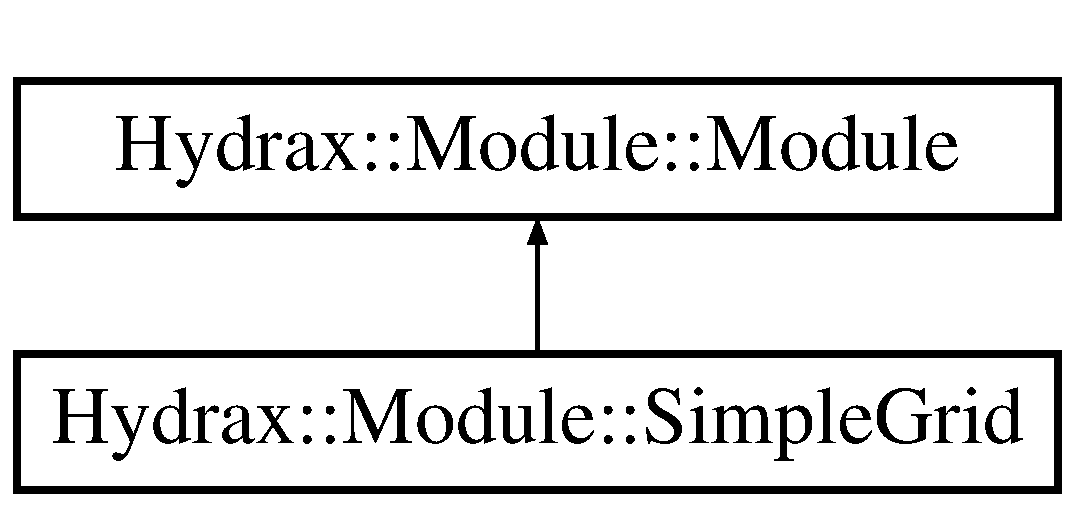
\includegraphics[height=2cm]{class_hydrax_1_1_module_1_1_simple_grid}
\end{center}
\end{figure}
\subsection*{Classes}
\begin{CompactItemize}
\item 
struct \hyperlink{struct_hydrax_1_1_module_1_1_simple_grid_1_1_options}{Options}
\end{CompactItemize}
\subsection*{Public Member Functions}
\begin{CompactItemize}
\item 
\hyperlink{class_hydrax_1_1_module_1_1_simple_grid_1576c59a302b3c24ac3d7dd8598e608c}{SimpleGrid} (\hyperlink{class_hydrax_1_1_hydrax}{Hydrax} $\ast$h, \hyperlink{class_hydrax_1_1_noise_1_1_noise}{Noise::Noise} $\ast$n, const \hyperlink{class_hydrax_1_1_material_manager_aa14689cd1c259f48954dfecda9b296f}{MaterialManager::NormalMode} \&NormalMode)
\item 
\hyperlink{class_hydrax_1_1_module_1_1_simple_grid_ae091cd103798dcc8f8b92af7dbfccef}{SimpleGrid} (\hyperlink{class_hydrax_1_1_hydrax}{Hydrax} $\ast$h, \hyperlink{class_hydrax_1_1_noise_1_1_noise}{Noise::Noise} $\ast$n, const \hyperlink{class_hydrax_1_1_material_manager_aa14689cd1c259f48954dfecda9b296f}{MaterialManager::NormalMode} \&NormalMode, const \hyperlink{struct_hydrax_1_1_module_1_1_simple_grid_1_1_options}{Options} \&\hyperlink{struct_hydrax_1_1_module_1_1_simple_grid_1_1_options}{Options})
\item 
\hyperlink{class_hydrax_1_1_module_1_1_simple_grid_a697faa687d55e5f211bae56e0ec9d14}{$\sim$SimpleGrid} ()
\item 
void \hyperlink{class_hydrax_1_1_module_1_1_simple_grid_7e52fb7497f6a2d27666a384d7a1d003}{create} ()
\item 
void \hyperlink{class_hydrax_1_1_module_1_1_simple_grid_ca3e257313599b797b8a65442cecd3cc}{remove} ()
\item 
void \hyperlink{class_hydrax_1_1_module_1_1_simple_grid_aa120d4f487785136a3134cc8980fb16}{update} (const Ogre::Real \&timeSinceLastFrame)
\item 
void \hyperlink{class_hydrax_1_1_module_1_1_simple_grid_6b83cb95b2803b068a53bf76afaa9ac4}{setOptions} (const \hyperlink{struct_hydrax_1_1_module_1_1_simple_grid_1_1_options}{Options} \&\hyperlink{struct_hydrax_1_1_module_1_1_simple_grid_1_1_options}{Options})
\item 
void \hyperlink{class_hydrax_1_1_module_1_1_simple_grid_f79cb3a457da1fe8b015d9d7b5a6a376}{saveCfg} (Ogre::String \&Data)
\item 
bool \hyperlink{class_hydrax_1_1_module_1_1_simple_grid_3741ec1a3df1863e730711fd9d3b14e1}{loadCfg} (Ogre::ConfigFile \&CfgFile)
\item 
float \hyperlink{class_hydrax_1_1_module_1_1_simple_grid_9a9e5bba632f0317c82370fa433559ac}{getHeigth} (const Ogre::Vector2 \&Position)
\item 
const \hyperlink{struct_hydrax_1_1_module_1_1_simple_grid_1_1_options}{Options} \& \hyperlink{class_hydrax_1_1_module_1_1_simple_grid_bcc8d6a849224e8558162adb8f3baf69}{getOptions} () const 
\end{CompactItemize}


\subsection{Detailed Description}
\hyperlink{class_hydrax_1_1_hydrax}{Hydrax} simple grid module 

\subsection{Constructor \& Destructor Documentation}
\hypertarget{class_hydrax_1_1_module_1_1_simple_grid_1576c59a302b3c24ac3d7dd8598e608c}{
\index{Hydrax::Module::SimpleGrid@{Hydrax::Module::SimpleGrid}!SimpleGrid@{SimpleGrid}}
\index{SimpleGrid@{SimpleGrid}!Hydrax::Module::SimpleGrid@{Hydrax::Module::SimpleGrid}}
\subsubsection[{SimpleGrid}]{\setlength{\rightskip}{0pt plus 5cm}Hydrax::Module::SimpleGrid::SimpleGrid ({\bf Hydrax} $\ast$ {\em h}, \/  {\bf Noise::Noise} $\ast$ {\em n}, \/  const {\bf MaterialManager::NormalMode} \& {\em NormalMode})}}
\label{class_hydrax_1_1_module_1_1_simple_grid_1576c59a302b3c24ac3d7dd8598e608c}


Constructor \begin{Desc}
\item[Parameters:]
\begin{description}
\item[{\em h}]\hyperlink{class_hydrax_1_1_hydrax}{Hydrax} manager pointer \item[{\em n}]\hyperlink{class_hydrax_1_1_hydrax}{Hydrax} noise module \item[{\em NormalMode}]Switch between \hyperlink{class_hydrax_1_1_material_manager_aa14689cd1c259f48954dfecda9b296ffe4d6257f673cf503a9905fb2576288f}{MaterialManager::NM\_\-VERTEX} and Materialmanager::NM\_\-RTT \end{description}
\end{Desc}
\hypertarget{class_hydrax_1_1_module_1_1_simple_grid_ae091cd103798dcc8f8b92af7dbfccef}{
\index{Hydrax::Module::SimpleGrid@{Hydrax::Module::SimpleGrid}!SimpleGrid@{SimpleGrid}}
\index{SimpleGrid@{SimpleGrid}!Hydrax::Module::SimpleGrid@{Hydrax::Module::SimpleGrid}}
\subsubsection[{SimpleGrid}]{\setlength{\rightskip}{0pt plus 5cm}Hydrax::Module::SimpleGrid::SimpleGrid ({\bf Hydrax} $\ast$ {\em h}, \/  {\bf Noise::Noise} $\ast$ {\em n}, \/  const {\bf MaterialManager::NormalMode} \& {\em NormalMode}, \/  const {\bf Options} \& {\em Options})}}
\label{class_hydrax_1_1_module_1_1_simple_grid_ae091cd103798dcc8f8b92af7dbfccef}


Constructor \begin{Desc}
\item[Parameters:]
\begin{description}
\item[{\em h}]\hyperlink{class_hydrax_1_1_hydrax}{Hydrax} manager pointer \item[{\em n}]\hyperlink{class_hydrax_1_1_hydrax}{Hydrax} noise module \item[{\em NormalMode}]Switch between \hyperlink{class_hydrax_1_1_material_manager_aa14689cd1c259f48954dfecda9b296ffe4d6257f673cf503a9905fb2576288f}{MaterialManager::NM\_\-VERTEX} and Materialmanager::NM\_\-RTT \item[{\em \hyperlink{struct_hydrax_1_1_module_1_1_simple_grid_1_1_options}{Options}}]Perlin options \end{description}
\end{Desc}
\hypertarget{class_hydrax_1_1_module_1_1_simple_grid_a697faa687d55e5f211bae56e0ec9d14}{
\index{Hydrax::Module::SimpleGrid@{Hydrax::Module::SimpleGrid}!$\sim$SimpleGrid@{$\sim$SimpleGrid}}
\index{$\sim$SimpleGrid@{$\sim$SimpleGrid}!Hydrax::Module::SimpleGrid@{Hydrax::Module::SimpleGrid}}
\subsubsection[{$\sim$SimpleGrid}]{\setlength{\rightskip}{0pt plus 5cm}Hydrax::Module::SimpleGrid::$\sim$SimpleGrid ()}}
\label{class_hydrax_1_1_module_1_1_simple_grid_a697faa687d55e5f211bae56e0ec9d14}


Destructor 

\subsection{Member Function Documentation}
\hypertarget{class_hydrax_1_1_module_1_1_simple_grid_7e52fb7497f6a2d27666a384d7a1d003}{
\index{Hydrax::Module::SimpleGrid@{Hydrax::Module::SimpleGrid}!create@{create}}
\index{create@{create}!Hydrax::Module::SimpleGrid@{Hydrax::Module::SimpleGrid}}
\subsubsection[{create}]{\setlength{\rightskip}{0pt plus 5cm}void Hydrax::Module::SimpleGrid::create ()\hspace{0.3cm}{\tt  \mbox{[}virtual\mbox{]}}}}
\label{class_hydrax_1_1_module_1_1_simple_grid_7e52fb7497f6a2d27666a384d7a1d003}


Create 

Reimplemented from \hyperlink{class_hydrax_1_1_module_1_1_module_4b696328c3fc1496f757e929f44f3258}{Hydrax::Module::Module}.\hypertarget{class_hydrax_1_1_module_1_1_simple_grid_9a9e5bba632f0317c82370fa433559ac}{
\index{Hydrax::Module::SimpleGrid@{Hydrax::Module::SimpleGrid}!getHeigth@{getHeigth}}
\index{getHeigth@{getHeigth}!Hydrax::Module::SimpleGrid@{Hydrax::Module::SimpleGrid}}
\subsubsection[{getHeigth}]{\setlength{\rightskip}{0pt plus 5cm}float Hydrax::Module::SimpleGrid::getHeigth (const Ogre::Vector2 \& {\em Position})\hspace{0.3cm}{\tt  \mbox{[}virtual\mbox{]}}}}
\label{class_hydrax_1_1_module_1_1_simple_grid_9a9e5bba632f0317c82370fa433559ac}


Get the current heigth at a especified world-space point \begin{Desc}
\item[Parameters:]
\begin{description}
\item[{\em Position}]X/Z World position \end{description}
\end{Desc}
\begin{Desc}
\item[Returns:]Heigth at the given position in y-World coordinates, if it's outside of the water return -1 \end{Desc}


Reimplemented from \hyperlink{class_hydrax_1_1_module_1_1_module_c61f89589d3b1bc7256731ddb7af7d0b}{Hydrax::Module::Module}.\hypertarget{class_hydrax_1_1_module_1_1_simple_grid_bcc8d6a849224e8558162adb8f3baf69}{
\index{Hydrax::Module::SimpleGrid@{Hydrax::Module::SimpleGrid}!getOptions@{getOptions}}
\index{getOptions@{getOptions}!Hydrax::Module::SimpleGrid@{Hydrax::Module::SimpleGrid}}
\subsubsection[{getOptions}]{\setlength{\rightskip}{0pt plus 5cm}const {\bf Options}\& Hydrax::Module::SimpleGrid::getOptions () const\hspace{0.3cm}{\tt  \mbox{[}inline\mbox{]}}}}
\label{class_hydrax_1_1_module_1_1_simple_grid_bcc8d6a849224e8558162adb8f3baf69}


Get current options \begin{Desc}
\item[Returns:]Current options \end{Desc}
\hypertarget{class_hydrax_1_1_module_1_1_simple_grid_3741ec1a3df1863e730711fd9d3b14e1}{
\index{Hydrax::Module::SimpleGrid@{Hydrax::Module::SimpleGrid}!loadCfg@{loadCfg}}
\index{loadCfg@{loadCfg}!Hydrax::Module::SimpleGrid@{Hydrax::Module::SimpleGrid}}
\subsubsection[{loadCfg}]{\setlength{\rightskip}{0pt plus 5cm}bool Hydrax::Module::SimpleGrid::loadCfg (Ogre::ConfigFile \& {\em CfgFile})\hspace{0.3cm}{\tt  \mbox{[}virtual\mbox{]}}}}
\label{class_hydrax_1_1_module_1_1_simple_grid_3741ec1a3df1863e730711fd9d3b14e1}


Load config \begin{Desc}
\item[Parameters:]
\begin{description}
\item[{\em CgfFile}]Ogre::ConfigFile reference \end{description}
\end{Desc}
\begin{Desc}
\item[Returns:]True if is the correct module config \end{Desc}


Reimplemented from \hyperlink{class_hydrax_1_1_module_1_1_module_bedb96357608c0744bb7816ae1c2b0bb}{Hydrax::Module::Module}.\hypertarget{class_hydrax_1_1_module_1_1_simple_grid_ca3e257313599b797b8a65442cecd3cc}{
\index{Hydrax::Module::SimpleGrid@{Hydrax::Module::SimpleGrid}!remove@{remove}}
\index{remove@{remove}!Hydrax::Module::SimpleGrid@{Hydrax::Module::SimpleGrid}}
\subsubsection[{remove}]{\setlength{\rightskip}{0pt plus 5cm}void Hydrax::Module::SimpleGrid::remove ()\hspace{0.3cm}{\tt  \mbox{[}virtual\mbox{]}}}}
\label{class_hydrax_1_1_module_1_1_simple_grid_ca3e257313599b797b8a65442cecd3cc}


Remove 

Reimplemented from \hyperlink{class_hydrax_1_1_module_1_1_module_21f60a53a99d72ff00d3fe5565518165}{Hydrax::Module::Module}.\hypertarget{class_hydrax_1_1_module_1_1_simple_grid_f79cb3a457da1fe8b015d9d7b5a6a376}{
\index{Hydrax::Module::SimpleGrid@{Hydrax::Module::SimpleGrid}!saveCfg@{saveCfg}}
\index{saveCfg@{saveCfg}!Hydrax::Module::SimpleGrid@{Hydrax::Module::SimpleGrid}}
\subsubsection[{saveCfg}]{\setlength{\rightskip}{0pt plus 5cm}void Hydrax::Module::SimpleGrid::saveCfg (Ogre::String \& {\em Data})\hspace{0.3cm}{\tt  \mbox{[}virtual\mbox{]}}}}
\label{class_hydrax_1_1_module_1_1_simple_grid_f79cb3a457da1fe8b015d9d7b5a6a376}


Save config \begin{Desc}
\item[Parameters:]
\begin{description}
\item[{\em Data}]String reference \end{description}
\end{Desc}


Reimplemented from \hyperlink{class_hydrax_1_1_module_1_1_module_998a5baf42f57b02ca7bc20bc12f95a9}{Hydrax::Module::Module}.\hypertarget{class_hydrax_1_1_module_1_1_simple_grid_6b83cb95b2803b068a53bf76afaa9ac4}{
\index{Hydrax::Module::SimpleGrid@{Hydrax::Module::SimpleGrid}!setOptions@{setOptions}}
\index{setOptions@{setOptions}!Hydrax::Module::SimpleGrid@{Hydrax::Module::SimpleGrid}}
\subsubsection[{setOptions}]{\setlength{\rightskip}{0pt plus 5cm}void Hydrax::Module::SimpleGrid::setOptions (const {\bf Options} \& {\em Options})}}
\label{class_hydrax_1_1_module_1_1_simple_grid_6b83cb95b2803b068a53bf76afaa9ac4}


Set options \begin{Desc}
\item[Parameters:]
\begin{description}
\item[{\em \hyperlink{struct_hydrax_1_1_module_1_1_simple_grid_1_1_options}{Options}}]\hyperlink{struct_hydrax_1_1_module_1_1_simple_grid_1_1_options}{Options} \end{description}
\end{Desc}
\hypertarget{class_hydrax_1_1_module_1_1_simple_grid_aa120d4f487785136a3134cc8980fb16}{
\index{Hydrax::Module::SimpleGrid@{Hydrax::Module::SimpleGrid}!update@{update}}
\index{update@{update}!Hydrax::Module::SimpleGrid@{Hydrax::Module::SimpleGrid}}
\subsubsection[{update}]{\setlength{\rightskip}{0pt plus 5cm}void Hydrax::Module::SimpleGrid::update (const Ogre::Real \& {\em timeSinceLastFrame})\hspace{0.3cm}{\tt  \mbox{[}virtual\mbox{]}}}}
\label{class_hydrax_1_1_module_1_1_simple_grid_aa120d4f487785136a3134cc8980fb16}


Call it each frame \begin{Desc}
\item[Parameters:]
\begin{description}
\item[{\em timeSinceLastFrame}]Time since last frame(delta) \end{description}
\end{Desc}


Reimplemented from \hyperlink{class_hydrax_1_1_module_1_1_module_2042d450f99d9348fa4b7bd29ba89df3}{Hydrax::Module::Module}.

The documentation for this class was generated from the following files:\begin{CompactItemize}
\item 
C:/Hydrax/v0.5.1/Hydrax/src/Hydrax/Modules/SimpleGrid/\hyperlink{_simple_grid_8h}{SimpleGrid.h}\item 
C:/Hydrax/v0.5.1/Hydrax/src/Hydrax/Modules/SimpleGrid/\hyperlink{_simple_grid_8cpp}{SimpleGrid.cpp}\end{CompactItemize}

\hypertarget{struct_hydrax_1_1_module_1_1_simple_grid_1_1_options}{
\section{Hydrax::Module::SimpleGrid::SimpleGrid::Options Struct Reference}
\label{struct_hydrax_1_1_module_1_1_simple_grid_1_1_options}\index{Hydrax::Module::SimpleGrid::Options@{Hydrax::Module::SimpleGrid::Options}}
}
{\tt \#include $<$SimpleGrid.h$>$}

\subsection*{Public Member Functions}
\begin{CompactItemize}
\item 
\hyperlink{struct_hydrax_1_1_module_1_1_simple_grid_1_1_options_e94dd7d6ad74998702368e88b44c35da}{Options} ()
\item 
\hyperlink{struct_hydrax_1_1_module_1_1_simple_grid_1_1_options_dfe5943bb6ad1703de7b40a721e3c316}{Options} (const int \&\_\-Complexity, const \hyperlink{struct_hydrax_1_1_size}{Size} \&\_\-MeshSize)
\item 
\hyperlink{struct_hydrax_1_1_module_1_1_simple_grid_1_1_options_5ed872d6df7b71b6e9a796946f995916}{Options} (const int \&\_\-Complexity, const \hyperlink{struct_hydrax_1_1_size}{Size} \&\_\-MeshSize, const float \&\_\-Strength, const bool \&\_\-Smooth, const bool \&\_\-ChoppyWaves, const float \&\_\-ChoppyStrength)
\end{CompactItemize}
\subsection*{Public Attributes}
\begin{CompactItemize}
\item 
int \hyperlink{struct_hydrax_1_1_module_1_1_simple_grid_1_1_options_3ccaa20a5351a3bd3e743f179a347e4f}{Complexity}
\begin{CompactList}\small\item\em Projected grid complexity (N$\ast$N). \item\end{CompactList}\item 
\hyperlink{struct_hydrax_1_1_size}{Size} \hyperlink{struct_hydrax_1_1_module_1_1_simple_grid_1_1_options_bb708bb0feb25558278a50492f593f0b}{MeshSize}
\begin{CompactList}\small\item\em \hyperlink{struct_hydrax_1_1_size}{Size}. \item\end{CompactList}\item 
float \hyperlink{struct_hydrax_1_1_module_1_1_simple_grid_1_1_options_35fd961ca7eeb63127378321c6b205a0}{Strength}
\begin{CompactList}\small\item\em Strength. \item\end{CompactList}\item 
bool \hyperlink{struct_hydrax_1_1_module_1_1_simple_grid_1_1_options_3b26b3400f42d6e753f5e00e7b7a8180}{Smooth}
\begin{CompactList}\small\item\em Smooth. \item\end{CompactList}\item 
bool \hyperlink{struct_hydrax_1_1_module_1_1_simple_grid_1_1_options_9cd5aefce26c64d689ee441431d47cc9}{ChoppyWaves}
\begin{CompactList}\small\item\em Choppy waves. \item\end{CompactList}\item 
float \hyperlink{struct_hydrax_1_1_module_1_1_simple_grid_1_1_options_2eda0cfbbe201148b3f3287ce4a91055}{ChoppyStrength}
\begin{CompactList}\small\item\em Choppy waves strength. \item\end{CompactList}\end{CompactItemize}


\subsection{Detailed Description}
Struct wich contains \hyperlink{class_hydrax_1_1_hydrax}{Hydrax} simple grid module options 

\subsection{Constructor \& Destructor Documentation}
\hypertarget{struct_hydrax_1_1_module_1_1_simple_grid_1_1_options_e94dd7d6ad74998702368e88b44c35da}{
\index{Hydrax::Module::SimpleGrid::Options@{Hydrax::Module::SimpleGrid::Options}!Options@{Options}}
\index{Options@{Options}!Hydrax::Module::SimpleGrid::Options@{Hydrax::Module::SimpleGrid::Options}}
\subsubsection[{Options}]{\setlength{\rightskip}{0pt plus 5cm}Hydrax::Module::SimpleGrid::SimpleGrid::Options::Options ()\hspace{0.3cm}{\tt  \mbox{[}inline\mbox{]}}}}
\label{struct_hydrax_1_1_module_1_1_simple_grid_1_1_options_e94dd7d6ad74998702368e88b44c35da}


Default constructor \hypertarget{struct_hydrax_1_1_module_1_1_simple_grid_1_1_options_dfe5943bb6ad1703de7b40a721e3c316}{
\index{Hydrax::Module::SimpleGrid::Options@{Hydrax::Module::SimpleGrid::Options}!Options@{Options}}
\index{Options@{Options}!Hydrax::Module::SimpleGrid::Options@{Hydrax::Module::SimpleGrid::Options}}
\subsubsection[{Options}]{\setlength{\rightskip}{0pt plus 5cm}Hydrax::Module::SimpleGrid::SimpleGrid::Options::Options (const int \& {\em \_\-Complexity}, \/  const {\bf Size} \& {\em \_\-MeshSize})\hspace{0.3cm}{\tt  \mbox{[}inline\mbox{]}}}}
\label{struct_hydrax_1_1_module_1_1_simple_grid_1_1_options_dfe5943bb6ad1703de7b40a721e3c316}


Constructor \begin{Desc}
\item[Parameters:]
\begin{description}
\item[{\em \_\-Complexity}]Projected grid complexity \item[{\em \_\-MeshSize}]Water mesh size \end{description}
\end{Desc}
\hypertarget{struct_hydrax_1_1_module_1_1_simple_grid_1_1_options_5ed872d6df7b71b6e9a796946f995916}{
\index{Hydrax::Module::SimpleGrid::Options@{Hydrax::Module::SimpleGrid::Options}!Options@{Options}}
\index{Options@{Options}!Hydrax::Module::SimpleGrid::Options@{Hydrax::Module::SimpleGrid::Options}}
\subsubsection[{Options}]{\setlength{\rightskip}{0pt plus 5cm}Hydrax::Module::SimpleGrid::SimpleGrid::Options::Options (const int \& {\em \_\-Complexity}, \/  const {\bf Size} \& {\em \_\-MeshSize}, \/  const float \& {\em \_\-Strength}, \/  const bool \& {\em \_\-Smooth}, \/  const bool \& {\em \_\-ChoppyWaves}, \/  const float \& {\em \_\-ChoppyStrength})\hspace{0.3cm}{\tt  \mbox{[}inline\mbox{]}}}}
\label{struct_hydrax_1_1_module_1_1_simple_grid_1_1_options_5ed872d6df7b71b6e9a796946f995916}


Constructor \begin{Desc}
\item[Parameters:]
\begin{description}
\item[{\em \_\-Complexity}]Projected grid complexity \item[{\em \_\-MeshSize}]Water mesh size \item[{\em \_\-Strength}]Perlin noise strength \item[{\em \_\-Smooth}]Smooth vertex? \item[{\em \_\-ChoppyWaves}]Choppy waves enabled? Note: Only with Materialmanager::NM\_\-VERTEX normal mode. \item[{\em \_\-ChoppyStrength}]Choppy waves strength Note: Only with Materialmanager::NM\_\-VERTEX normal mode. \end{description}
\end{Desc}


\subsection{Member Data Documentation}
\hypertarget{struct_hydrax_1_1_module_1_1_simple_grid_1_1_options_2eda0cfbbe201148b3f3287ce4a91055}{
\index{Hydrax::Module::SimpleGrid::Options@{Hydrax::Module::SimpleGrid::Options}!ChoppyStrength@{ChoppyStrength}}
\index{ChoppyStrength@{ChoppyStrength}!Hydrax::Module::SimpleGrid::Options@{Hydrax::Module::SimpleGrid::Options}}
\subsubsection[{ChoppyStrength}]{\setlength{\rightskip}{0pt plus 5cm}float Hydrax::Module::SimpleGrid::SimpleGrid::Options::ChoppyStrength}}
\label{struct_hydrax_1_1_module_1_1_simple_grid_1_1_options_2eda0cfbbe201148b3f3287ce4a91055}


Choppy waves strength. 

\hypertarget{struct_hydrax_1_1_module_1_1_simple_grid_1_1_options_9cd5aefce26c64d689ee441431d47cc9}{
\index{Hydrax::Module::SimpleGrid::Options@{Hydrax::Module::SimpleGrid::Options}!ChoppyWaves@{ChoppyWaves}}
\index{ChoppyWaves@{ChoppyWaves}!Hydrax::Module::SimpleGrid::Options@{Hydrax::Module::SimpleGrid::Options}}
\subsubsection[{ChoppyWaves}]{\setlength{\rightskip}{0pt plus 5cm}bool Hydrax::Module::SimpleGrid::SimpleGrid::Options::ChoppyWaves}}
\label{struct_hydrax_1_1_module_1_1_simple_grid_1_1_options_9cd5aefce26c64d689ee441431d47cc9}


Choppy waves. 

\hypertarget{struct_hydrax_1_1_module_1_1_simple_grid_1_1_options_3ccaa20a5351a3bd3e743f179a347e4f}{
\index{Hydrax::Module::SimpleGrid::Options@{Hydrax::Module::SimpleGrid::Options}!Complexity@{Complexity}}
\index{Complexity@{Complexity}!Hydrax::Module::SimpleGrid::Options@{Hydrax::Module::SimpleGrid::Options}}
\subsubsection[{Complexity}]{\setlength{\rightskip}{0pt plus 5cm}int Hydrax::Module::SimpleGrid::SimpleGrid::Options::Complexity}}
\label{struct_hydrax_1_1_module_1_1_simple_grid_1_1_options_3ccaa20a5351a3bd3e743f179a347e4f}


Projected grid complexity (N$\ast$N). 

\hypertarget{struct_hydrax_1_1_module_1_1_simple_grid_1_1_options_bb708bb0feb25558278a50492f593f0b}{
\index{Hydrax::Module::SimpleGrid::Options@{Hydrax::Module::SimpleGrid::Options}!MeshSize@{MeshSize}}
\index{MeshSize@{MeshSize}!Hydrax::Module::SimpleGrid::Options@{Hydrax::Module::SimpleGrid::Options}}
\subsubsection[{MeshSize}]{\setlength{\rightskip}{0pt plus 5cm}{\bf Size} Hydrax::Module::SimpleGrid::SimpleGrid::Options::MeshSize}}
\label{struct_hydrax_1_1_module_1_1_simple_grid_1_1_options_bb708bb0feb25558278a50492f593f0b}


\hyperlink{struct_hydrax_1_1_size}{Size}. 

\hypertarget{struct_hydrax_1_1_module_1_1_simple_grid_1_1_options_3b26b3400f42d6e753f5e00e7b7a8180}{
\index{Hydrax::Module::SimpleGrid::Options@{Hydrax::Module::SimpleGrid::Options}!Smooth@{Smooth}}
\index{Smooth@{Smooth}!Hydrax::Module::SimpleGrid::Options@{Hydrax::Module::SimpleGrid::Options}}
\subsubsection[{Smooth}]{\setlength{\rightskip}{0pt plus 5cm}bool Hydrax::Module::SimpleGrid::SimpleGrid::Options::Smooth}}
\label{struct_hydrax_1_1_module_1_1_simple_grid_1_1_options_3b26b3400f42d6e753f5e00e7b7a8180}


Smooth. 

\hypertarget{struct_hydrax_1_1_module_1_1_simple_grid_1_1_options_35fd961ca7eeb63127378321c6b205a0}{
\index{Hydrax::Module::SimpleGrid::Options@{Hydrax::Module::SimpleGrid::Options}!Strength@{Strength}}
\index{Strength@{Strength}!Hydrax::Module::SimpleGrid::Options@{Hydrax::Module::SimpleGrid::Options}}
\subsubsection[{Strength}]{\setlength{\rightskip}{0pt plus 5cm}float Hydrax::Module::SimpleGrid::SimpleGrid::Options::Strength}}
\label{struct_hydrax_1_1_module_1_1_simple_grid_1_1_options_35fd961ca7eeb63127378321c6b205a0}


Strength. 



The documentation for this struct was generated from the following file:\begin{CompactItemize}
\item 
C:/Hydrax/v0.5.1/Hydrax/src/Hydrax/Modules/SimpleGrid/\hyperlink{_simple_grid_8h}{SimpleGrid.h}\end{CompactItemize}

\hypertarget{struct_hydrax_1_1_size}{
\section{Hydrax::Size Struct Reference}
\label{struct_hydrax_1_1_size}\index{Hydrax::Size@{Hydrax::Size}}
}
{\tt \#include $<$Help.h$>$}

\subsection*{Public Member Functions}
\begin{CompactItemize}
\item 
\hyperlink{struct_hydrax_1_1_size_39cf079297d9a43d89c71e6fbd5ade83}{Size} ()
\item 
\hyperlink{struct_hydrax_1_1_size_551027687e3c4646e6887df821ff9e1b}{Size} (const int \&size)
\item 
\hyperlink{struct_hydrax_1_1_size_a4a9f0e492ed8f602f6f5e5955042464}{Size} (const int \&width, const int \&height)
\item 
\hyperlink{struct_hydrax_1_1_size_ace8e593f9b2c5f6672f401ba86a2df9}{$\sim$Size} ()
\item 
void \hyperlink{struct_hydrax_1_1_size_ed24a854ee32305fda00bd0c41fa2d0a}{setSize} (const int \&size)
\item 
void \hyperlink{struct_hydrax_1_1_size_a8ab07e13e4931f071f6af2161728168}{setSize} (const int \&width, const int \&height)
\end{CompactItemize}
\subsection*{Public Attributes}
\begin{CompactItemize}
\item 
int \hyperlink{struct_hydrax_1_1_size_5dfca2c4f9a35424d03dfbbe34da0b84}{Width}
\begin{CompactList}\small\item\em Width value. \item\end{CompactList}\item 
int \hyperlink{struct_hydrax_1_1_size_24e29f4f28eb941f06d9f424807691e6}{Height}
\begin{CompactList}\small\item\em Height value. \item\end{CompactList}\end{CompactItemize}


\subsection{Detailed Description}
Struct wich contains an especific width and height value 

\subsection{Constructor \& Destructor Documentation}
\hypertarget{struct_hydrax_1_1_size_39cf079297d9a43d89c71e6fbd5ade83}{
\index{Hydrax::Size@{Hydrax::Size}!Size@{Size}}
\index{Size@{Size}!Hydrax::Size@{Hydrax::Size}}
\subsubsection[{Size}]{\setlength{\rightskip}{0pt plus 5cm}Hydrax::Size::Size ()\hspace{0.3cm}{\tt  \mbox{[}inline\mbox{]}}}}
\label{struct_hydrax_1_1_size_39cf079297d9a43d89c71e6fbd5ade83}


Default constructor \hypertarget{struct_hydrax_1_1_size_551027687e3c4646e6887df821ff9e1b}{
\index{Hydrax::Size@{Hydrax::Size}!Size@{Size}}
\index{Size@{Size}!Hydrax::Size@{Hydrax::Size}}
\subsubsection[{Size}]{\setlength{\rightskip}{0pt plus 5cm}Hydrax::Size::Size (const int \& {\em size})\hspace{0.3cm}{\tt  \mbox{[}inline\mbox{]}}}}
\label{struct_hydrax_1_1_size_551027687e3c4646e6887df821ff9e1b}


Constructor \begin{Desc}
\item[Parameters:]
\begin{description}
\item[{\em size}]The width and height values \end{description}
\end{Desc}
\hypertarget{struct_hydrax_1_1_size_a4a9f0e492ed8f602f6f5e5955042464}{
\index{Hydrax::Size@{Hydrax::Size}!Size@{Size}}
\index{Size@{Size}!Hydrax::Size@{Hydrax::Size}}
\subsubsection[{Size}]{\setlength{\rightskip}{0pt plus 5cm}Hydrax::Size::Size (const int \& {\em width}, \/  const int \& {\em height})\hspace{0.3cm}{\tt  \mbox{[}inline\mbox{]}}}}
\label{struct_hydrax_1_1_size_a4a9f0e492ed8f602f6f5e5955042464}


Constructor \begin{Desc}
\item[Parameters:]
\begin{description}
\item[{\em width}]Width value \item[{\em height}]Height value \end{description}
\end{Desc}
\hypertarget{struct_hydrax_1_1_size_ace8e593f9b2c5f6672f401ba86a2df9}{
\index{Hydrax::Size@{Hydrax::Size}!$\sim$Size@{$\sim$Size}}
\index{$\sim$Size@{$\sim$Size}!Hydrax::Size@{Hydrax::Size}}
\subsubsection[{$\sim$Size}]{\setlength{\rightskip}{0pt plus 5cm}Hydrax::Size::$\sim$Size ()\hspace{0.3cm}{\tt  \mbox{[}inline\mbox{]}}}}
\label{struct_hydrax_1_1_size_ace8e593f9b2c5f6672f401ba86a2df9}


Destructor 

\subsection{Member Function Documentation}
\hypertarget{struct_hydrax_1_1_size_a8ab07e13e4931f071f6af2161728168}{
\index{Hydrax::Size@{Hydrax::Size}!setSize@{setSize}}
\index{setSize@{setSize}!Hydrax::Size@{Hydrax::Size}}
\subsubsection[{setSize}]{\setlength{\rightskip}{0pt plus 5cm}void Hydrax::Size::setSize (const int \& {\em width}, \/  const int \& {\em height})\hspace{0.3cm}{\tt  \mbox{[}inline\mbox{]}}}}
\label{struct_hydrax_1_1_size_a8ab07e13e4931f071f6af2161728168}


Sets the especified values \begin{Desc}
\item[Parameters:]
\begin{description}
\item[{\em width}]Width value \item[{\em height}]Height value \end{description}
\end{Desc}
\hypertarget{struct_hydrax_1_1_size_ed24a854ee32305fda00bd0c41fa2d0a}{
\index{Hydrax::Size@{Hydrax::Size}!setSize@{setSize}}
\index{setSize@{setSize}!Hydrax::Size@{Hydrax::Size}}
\subsubsection[{setSize}]{\setlength{\rightskip}{0pt plus 5cm}void Hydrax::Size::setSize (const int \& {\em size})\hspace{0.3cm}{\tt  \mbox{[}inline\mbox{]}}}}
\label{struct_hydrax_1_1_size_ed24a854ee32305fda00bd0c41fa2d0a}


Sets the same width and height value \begin{Desc}
\item[Parameters:]
\begin{description}
\item[{\em size}]The width and height values \end{description}
\end{Desc}


\subsection{Member Data Documentation}
\hypertarget{struct_hydrax_1_1_size_24e29f4f28eb941f06d9f424807691e6}{
\index{Hydrax::Size@{Hydrax::Size}!Height@{Height}}
\index{Height@{Height}!Hydrax::Size@{Hydrax::Size}}
\subsubsection[{Height}]{\setlength{\rightskip}{0pt plus 5cm}int {\bf Hydrax::Size::Height}}}
\label{struct_hydrax_1_1_size_24e29f4f28eb941f06d9f424807691e6}


Height value. 

\hypertarget{struct_hydrax_1_1_size_5dfca2c4f9a35424d03dfbbe34da0b84}{
\index{Hydrax::Size@{Hydrax::Size}!Width@{Width}}
\index{Width@{Width}!Hydrax::Size@{Hydrax::Size}}
\subsubsection[{Width}]{\setlength{\rightskip}{0pt plus 5cm}int {\bf Hydrax::Size::Width}}}
\label{struct_hydrax_1_1_size_5dfca2c4f9a35424d03dfbbe34da0b84}


Width value. 



The documentation for this struct was generated from the following file:\begin{CompactItemize}
\item 
C:/Hydrax/v0.5.1/Hydrax/src/Hydrax/\hyperlink{_help_8h}{Help.h}\end{CompactItemize}

\hypertarget{class_hydrax_1_1_texture_manager}{
\section{Hydrax::TextureManager Class Reference}
\label{class_hydrax_1_1_texture_manager}\index{Hydrax::TextureManager@{Hydrax::TextureManager}}
}
{\tt \#include $<$TextureManager.h$>$}

\subsection*{Public Types}
\begin{CompactItemize}
\item 
enum \hyperlink{class_hydrax_1_1_texture_manager_9af2a9718c00e64eb188c3dd9cd0fd04}{TexturesID} \{ \hyperlink{class_hydrax_1_1_texture_manager_9af2a9718c00e64eb188c3dd9cd0fd04f04e9f7557359214c8000825a6b75922}{TEX\_\-NORMAL\_\-ID} =  0
 \}
\subsection*{Public Member Functions}
\begin{CompactItemize}
\item 
\hyperlink{class_hydrax_1_1_texture_manager_bad81d53663c93a5d2d9bd49eff0ef90}{TextureManager} (\hyperlink{class_hydrax_1_1_hydrax}{Hydrax} $\ast$h)
\item 
\hyperlink{class_hydrax_1_1_texture_manager_d7e356de2834c2f1668826f21c1dbf1d}{$\sim$TextureManager} ()
\item 
void \hyperlink{class_hydrax_1_1_texture_manager_30bfb59332540e897c43193474b4aa19}{create} (const \hyperlink{struct_hydrax_1_1_size}{Size} \&\hyperlink{struct_hydrax_1_1_size}{Size})
\item 
void \hyperlink{class_hydrax_1_1_texture_manager_d6164d9f44096b59b15c92223be0752a}{remove} ()
\item 
bool \hyperlink{class_hydrax_1_1_texture_manager_eec28019cfbb7d4ec705b07d5519f98a}{update} (const \hyperlink{class_hydrax_1_1_texture_manager_9af2a9718c00e64eb188c3dd9cd0fd04}{TexturesID} \&Id, \hyperlink{class_hydrax_1_1_image}{Image} \&\hyperlink{class_hydrax_1_1_image}{Image})
\item 
Ogre::TexturePtr \& \hyperlink{class_hydrax_1_1_texture_manager_7f15f24a8ff1372f6a1840c27aec655f}{getTexture} (const \hyperlink{class_hydrax_1_1_texture_manager_9af2a9718c00e64eb188c3dd9cd0fd04}{TexturesID} \&Id)
\item 
const Ogre::String \& \hyperlink{class_hydrax_1_1_texture_manager_ba3bf13c7d3971c9cbf2b32c650d906e}{getTextureName} (const \hyperlink{class_hydrax_1_1_texture_manager_9af2a9718c00e64eb188c3dd9cd0fd04}{TexturesID} \&Id) const 
\end{CompactItemize}


\subsection{Detailed Description}
Class for manager Normal maps. 

\subsection{Member Enumeration Documentation}
\hypertarget{class_hydrax_1_1_texture_manager_9af2a9718c00e64eb188c3dd9cd0fd04}{
\index{Hydrax::TextureManager@{Hydrax::TextureManager}!TexturesID@{TexturesID}}
\index{TexturesID@{TexturesID}!Hydrax::TextureManager@{Hydrax::TextureManager}}
\subsubsection[{TexturesID}]{\setlength{\rightskip}{0pt plus 5cm}enum {\bf Hydrax::TextureManager::TexturesID}}}
\label{class_hydrax_1_1_texture_manager_9af2a9718c00e64eb188c3dd9cd0fd04}


Textures enumeration \begin{Desc}
\item[Enumerator: ]\par
\begin{description}
\index{TEX\_\-NORMAL\_\-ID@{TEX\_\-NORMAL\_\-ID}!Hydrax::TextureManager@{Hydrax::TextureManager}}\index{Hydrax::TextureManager@{Hydrax::TextureManager}!TEX\_\-NORMAL\_\-ID@{TEX\_\-NORMAL\_\-ID}}\item[{\em 
\hypertarget{class_hydrax_1_1_texture_manager_9af2a9718c00e64eb188c3dd9cd0fd04f04e9f7557359214c8000825a6b75922}{
TEX\_\-NORMAL\_\-ID}
\label{class_hydrax_1_1_texture_manager_9af2a9718c00e64eb188c3dd9cd0fd04f04e9f7557359214c8000825a6b75922}
}]\end{description}
\end{Desc}



\subsection{Constructor \& Destructor Documentation}
\hypertarget{class_hydrax_1_1_texture_manager_bad81d53663c93a5d2d9bd49eff0ef90}{
\index{Hydrax::TextureManager@{Hydrax::TextureManager}!TextureManager@{TextureManager}}
\index{TextureManager@{TextureManager}!Hydrax::TextureManager@{Hydrax::TextureManager}}
\subsubsection[{TextureManager}]{\setlength{\rightskip}{0pt plus 5cm}Hydrax::TextureManager::TextureManager ({\bf Hydrax} $\ast$ {\em h})}}
\label{class_hydrax_1_1_texture_manager_bad81d53663c93a5d2d9bd49eff0ef90}


Constructor \begin{Desc}
\item[Parameters:]
\begin{description}
\item[{\em h}]\hyperlink{class_hydrax_1_1_hydrax}{Hydrax} main pointer \end{description}
\end{Desc}
\hypertarget{class_hydrax_1_1_texture_manager_d7e356de2834c2f1668826f21c1dbf1d}{
\index{Hydrax::TextureManager@{Hydrax::TextureManager}!$\sim$TextureManager@{$\sim$TextureManager}}
\index{$\sim$TextureManager@{$\sim$TextureManager}!Hydrax::TextureManager@{Hydrax::TextureManager}}
\subsubsection[{$\sim$TextureManager}]{\setlength{\rightskip}{0pt plus 5cm}Hydrax::TextureManager::$\sim$TextureManager ()}}
\label{class_hydrax_1_1_texture_manager_d7e356de2834c2f1668826f21c1dbf1d}


Destructor 

\subsection{Member Function Documentation}
\hypertarget{class_hydrax_1_1_texture_manager_30bfb59332540e897c43193474b4aa19}{
\index{Hydrax::TextureManager@{Hydrax::TextureManager}!create@{create}}
\index{create@{create}!Hydrax::TextureManager@{Hydrax::TextureManager}}
\subsubsection[{create}]{\setlength{\rightskip}{0pt plus 5cm}void Hydrax::TextureManager::create (const {\bf Size} \& {\em Size})}}
\label{class_hydrax_1_1_texture_manager_30bfb59332540e897c43193474b4aa19}


Create height and normal map textures \begin{Desc}
\item[Parameters:]
\begin{description}
\item[{\em \hyperlink{struct_hydrax_1_1_size}{Size}}]Textures's size \end{description}
\end{Desc}
\hypertarget{class_hydrax_1_1_texture_manager_7f15f24a8ff1372f6a1840c27aec655f}{
\index{Hydrax::TextureManager@{Hydrax::TextureManager}!getTexture@{getTexture}}
\index{getTexture@{getTexture}!Hydrax::TextureManager@{Hydrax::TextureManager}}
\subsubsection[{getTexture}]{\setlength{\rightskip}{0pt plus 5cm}Ogre::TexturePtr\& Hydrax::TextureManager::getTexture (const {\bf TexturesID} \& {\em Id})\hspace{0.3cm}{\tt  \mbox{[}inline\mbox{]}}}}
\label{class_hydrax_1_1_texture_manager_7f15f24a8ff1372f6a1840c27aec655f}


Get texture \begin{Desc}
\item[Parameters:]
\begin{description}
\item[{\em Id}]Texture Id ( TEX\_\-NORMAL\_\-ID ) \end{description}
\end{Desc}
\begin{Desc}
\item[Returns:]Ogre::TexturePtr \end{Desc}
\hypertarget{class_hydrax_1_1_texture_manager_ba3bf13c7d3971c9cbf2b32c650d906e}{
\index{Hydrax::TextureManager@{Hydrax::TextureManager}!getTextureName@{getTextureName}}
\index{getTextureName@{getTextureName}!Hydrax::TextureManager@{Hydrax::TextureManager}}
\subsubsection[{getTextureName}]{\setlength{\rightskip}{0pt plus 5cm}const Ogre::String\& Hydrax::TextureManager::getTextureName (const {\bf TexturesID} \& {\em Id}) const\hspace{0.3cm}{\tt  \mbox{[}inline\mbox{]}}}}
\label{class_hydrax_1_1_texture_manager_ba3bf13c7d3971c9cbf2b32c650d906e}


Get texture's name \begin{Desc}
\item[Parameters:]
\begin{description}
\item[{\em Id}]Texture Id ( TEX\_\-NORMAL\_\-ID ) \end{description}
\end{Desc}
\begin{Desc}
\item[Returns:]Texture's name \end{Desc}
\hypertarget{class_hydrax_1_1_texture_manager_d6164d9f44096b59b15c92223be0752a}{
\index{Hydrax::TextureManager@{Hydrax::TextureManager}!remove@{remove}}
\index{remove@{remove}!Hydrax::TextureManager@{Hydrax::TextureManager}}
\subsubsection[{remove}]{\setlength{\rightskip}{0pt plus 5cm}void Hydrax::TextureManager::remove ()}}
\label{class_hydrax_1_1_texture_manager_d6164d9f44096b59b15c92223be0752a}


Remove textures \hypertarget{class_hydrax_1_1_texture_manager_eec28019cfbb7d4ec705b07d5519f98a}{
\index{Hydrax::TextureManager@{Hydrax::TextureManager}!update@{update}}
\index{update@{update}!Hydrax::TextureManager@{Hydrax::TextureManager}}
\subsubsection[{update}]{\setlength{\rightskip}{0pt plus 5cm}bool Hydrax::TextureManager::update (const {\bf TexturesID} \& {\em Id}, \/  {\bf Image} \& {\em Image})\hspace{0.3cm}{\tt  \mbox{[}inline\mbox{]}}}}
\label{class_hydrax_1_1_texture_manager_eec28019cfbb7d4ec705b07d5519f98a}


Update \begin{Desc}
\item[Parameters:]
\begin{description}
\item[{\em Id}]Texture's ID \item[{\em \hyperlink{class_hydrax_1_1_image}{Image}}]Update image \end{description}
\end{Desc}
\begin{Desc}
\item[Returns:]false if something fails \end{Desc}
\begin{Desc}
\item[Remarks:]If you need to update the texture with another way of data, get the Ogre::TexturePtr and modify it directly. Normal image will be Image::Type::TYPE\_\-RGB \mbox{[}0,255\mbox{]} range \end{Desc}


The documentation for this class was generated from the following files:\begin{CompactItemize}
\item 
C:/Hydrax/v0.5.1/Hydrax/src/Hydrax/\hyperlink{_texture_manager_8h}{TextureManager.h}\item 
C:/Hydrax/v0.5.1/Hydrax/src/Hydrax/\hyperlink{_texture_manager_8cpp}{TextureManager.cpp}\end{CompactItemize}

\chapter{File Documentation}
\hypertarget{_cfg_file_manager_8cpp}{
\section{C:/Hydrax/v0.5.1/Hydrax/src/Hydrax/CfgFileManager.cpp File Reference}
\label{_cfg_file_manager_8cpp}\index{C:/Hydrax/v0.5.1/Hydrax/src/Hydrax/CfgFileManager.cpp@{C:/Hydrax/v0.5.1/Hydrax/src/Hydrax/CfgFileManager.cpp}}
}
{\tt \#include \char`\"{}CfgFileManager.h\char`\"{}}\par
{\tt \#include \char`\"{}Hydrax.h\char`\"{}}\par
\subsection*{Namespaces}
\begin{CompactItemize}
\item 
namespace \hyperlink{namespace_hydrax}{Hydrax}
\end{CompactItemize}

\hypertarget{_cfg_file_manager_8h}{
\section{C:/Hydrax/v0.5.1/Hydrax/src/Hydrax/CfgFileManager.h File Reference}
\label{_cfg_file_manager_8h}\index{C:/Hydrax/v0.5.1/Hydrax/src/Hydrax/CfgFileManager.h@{C:/Hydrax/v0.5.1/Hydrax/src/Hydrax/CfgFileManager.h}}
}
{\tt \#include \char`\"{}Prerequisites.h\char`\"{}}\par
{\tt \#include \char`\"{}Help.h\char`\"{}}\par
\subsection*{Classes}
\begin{CompactItemize}
\item 
class \hyperlink{class_hydrax_1_1_cfg_file_manager}{Hydrax::CfgFileManager}
\end{CompactItemize}
\subsection*{Namespaces}
\begin{CompactItemize}
\item 
namespace \hyperlink{namespace_hydrax}{Hydrax}
\end{CompactItemize}

\hypertarget{_decals_manager_8cpp}{
\section{C:/Hydrax/v0.5.1/Hydrax/src/Hydrax/DecalsManager.cpp File Reference}
\label{_decals_manager_8cpp}\index{C:/Hydrax/v0.5.1/Hydrax/src/Hydrax/DecalsManager.cpp@{C:/Hydrax/v0.5.1/Hydrax/src/Hydrax/DecalsManager.cpp}}
}
{\tt \#include \char`\"{}DecalsManager.h\char`\"{}}\par
{\tt \#include \char`\"{}Hydrax.h\char`\"{}}\par
\subsection*{Namespaces}
\begin{CompactItemize}
\item 
namespace \hyperlink{namespace_hydrax}{Hydrax}
\end{CompactItemize}

\hypertarget{_decals_manager_8h}{
\section{C:/Hydrax/v0.5.1/Hydrax/src/Hydrax/DecalsManager.h File Reference}
\label{_decals_manager_8h}\index{C:/Hydrax/v0.5.1/Hydrax/src/Hydrax/DecalsManager.h@{C:/Hydrax/v0.5.1/Hydrax/src/Hydrax/DecalsManager.h}}
}
{\tt \#include \char`\"{}Prerequisites.h\char`\"{}}\par
\subsection*{Classes}
\begin{CompactItemize}
\item 
class \hyperlink{class_hydrax_1_1_decal}{Hydrax::Decal}
\item 
class \hyperlink{class_hydrax_1_1_decals_manager}{Hydrax::DecalsManager}
\end{CompactItemize}
\subsection*{Namespaces}
\begin{CompactItemize}
\item 
namespace \hyperlink{namespace_hydrax}{Hydrax}
\end{CompactItemize}

\hypertarget{_enums_8cpp}{
\section{C:/Hydrax/v0.5.1/Hydrax/src/Hydrax/Enums.cpp File Reference}
\label{_enums_8cpp}\index{C:/Hydrax/v0.5.1/Hydrax/src/Hydrax/Enums.cpp@{C:/Hydrax/v0.5.1/Hydrax/src/Hydrax/Enums.cpp}}
}
{\tt \#include \char`\"{}Enums.h\char`\"{}}\par
\subsection*{Namespaces}
\begin{CompactItemize}
\item 
namespace \hyperlink{namespace_hydrax}{Hydrax}
\end{CompactItemize}

\hypertarget{_enums_8h}{
\section{C:/Hydrax/v0.5.1/Hydrax/src/Hydrax/Enums.h File Reference}
\label{_enums_8h}\index{C:/Hydrax/v0.5.1/Hydrax/src/Hydrax/Enums.h@{C:/Hydrax/v0.5.1/Hydrax/src/Hydrax/Enums.h}}
}
{\tt \#include \char`\"{}Prerequisites.h\char`\"{}}\par
\subsection*{Namespaces}
\begin{CompactItemize}
\item 
namespace \hyperlink{namespace_hydrax}{Hydrax}
\end{CompactItemize}
\subsection*{Enumerations}
\begin{CompactItemize}
\item 
enum \hyperlink{namespace_hydrax_98bba1da65ee3695e9acde6904669070}{Hydrax::TextureQuality} \{ \par
\hyperlink{namespace_hydrax_98bba1da65ee3695e9acde690466907013824bd5f2e00064e13879a3aed066f7}{Hydrax::TEX\_\-QUA\_\-2} =  2, 
\hyperlink{namespace_hydrax_98bba1da65ee3695e9acde69046690702c54cb34b904921012f12bfed49a616c}{Hydrax::TEX\_\-QUA\_\-4} =  4, 
\hyperlink{namespace_hydrax_98bba1da65ee3695e9acde6904669070ecfa2867c6e6ff49c6fe3de1ee14dfb5}{Hydrax::TEX\_\-QUA\_\-8} =  8, 
\hyperlink{namespace_hydrax_98bba1da65ee3695e9acde690466907059ce2a1e784a9678d9fe8c53b17ff77a}{Hydrax::TEX\_\-QUA\_\-16} =  16, 
\par
\hyperlink{namespace_hydrax_98bba1da65ee3695e9acde6904669070213ee3a8654bbdf324b37c2aa7646955}{Hydrax::TEX\_\-QUA\_\-32} =  32, 
\hyperlink{namespace_hydrax_98bba1da65ee3695e9acde6904669070484d5d48abafe0b988868615a1ff2bfe}{Hydrax::TEX\_\-QUA\_\-64} =  64, 
\hyperlink{namespace_hydrax_98bba1da65ee3695e9acde69046690703356abd73b2ab0f647af5353fb0018f4}{Hydrax::TEX\_\-QUA\_\-128} =  128, 
\hyperlink{namespace_hydrax_98bba1da65ee3695e9acde6904669070060fdd6477e0aa66c348fe0969919d1b}{Hydrax::TEX\_\-QUA\_\-256} =  256, 
\par
\hyperlink{namespace_hydrax_98bba1da65ee3695e9acde69046690705ea2b7bdbf85bea10a3deae43d57644e}{Hydrax::TEX\_\-QUA\_\-512} =  512, 
\hyperlink{namespace_hydrax_98bba1da65ee3695e9acde6904669070f9e07a2b8439f2f9a113d777eb9afc00}{Hydrax::TEX\_\-QUA\_\-1024} =  1024
 \}
\item 
enum \hyperlink{namespace_hydrax_e8e15abf83a51b0cf514c7d1a133650a}{Hydrax::HydraxComponent} \{ \par
\hyperlink{namespace_hydrax_e8e15abf83a51b0cf514c7d1a133650ac4c50e1c15a4242bae28b68b1784f6cb}{Hydrax::HYDRAX\_\-COMPONENT\_\-SUN} =  1 $<$$<$ 0, 
\hyperlink{namespace_hydrax_e8e15abf83a51b0cf514c7d1a133650afbc9669fa36754e818079547219e3fd4}{Hydrax::HYDRAX\_\-COMPONENT\_\-FOAM} =  1 $<$$<$ 1, 
\hyperlink{namespace_hydrax_e8e15abf83a51b0cf514c7d1a133650a6589f4ae29b66557b9c0da80e563e710}{Hydrax::HYDRAX\_\-COMPONENT\_\-DEPTH} =  1 $<$$<$ 2, 
\hyperlink{namespace_hydrax_e8e15abf83a51b0cf514c7d1a133650a72cc575e7f40e9b5fe18cadcecd09b71}{Hydrax::HYDRAX\_\-COMPONENT\_\-SMOOTH} =  1 $<$$<$ 3, 
\par
\hyperlink{namespace_hydrax_e8e15abf83a51b0cf514c7d1a133650afe9facf191be0c10b4f69830f710fb14}{Hydrax::HYDRAX\_\-COMPONENT\_\-CAUSTICS} =  1 $<$$<$ 4, 
\hyperlink{namespace_hydrax_e8e15abf83a51b0cf514c7d1a133650aa254cfa1f4abfaf9346790b07a35230f}{Hydrax::HYDRAX\_\-COMPONENT\_\-UNDERWATER} =  1 $<$$<$ 5, 
\hyperlink{namespace_hydrax_e8e15abf83a51b0cf514c7d1a133650ad36eef3c9563ed01919fc80b392c1219}{Hydrax::HYDRAX\_\-COMPONENT\_\-UNDERWATER\_\-REFLECTIONS} =  1 $<$$<$ 6, 
\hyperlink{namespace_hydrax_e8e15abf83a51b0cf514c7d1a133650ac8c0ea85d7bb90af0bb5c86477ba713d}{Hydrax::HYDRAX\_\-COMPONENT\_\-UNDERWATER\_\-GODRAYS} =  1 $<$$<$ 7, 
\par
\hyperlink{namespace_hydrax_e8e15abf83a51b0cf514c7d1a133650a0b233091f338e451e5f5dc7477674ed2}{Hydrax::HYDRAX\_\-COMPONENTS\_\-NONE} =  0x0000, 
\hyperlink{namespace_hydrax_e8e15abf83a51b0cf514c7d1a133650a38ef11872d5d476e23224d209a114da8}{Hydrax::HYDRAX\_\-COMPONENTS\_\-ALL} =  0x001F
 \}
\end{CompactItemize}

\hypertarget{_god_rays_manager_8cpp}{
\section{C:/Hydrax/v0.5.1/Hydrax/src/Hydrax/GodRaysManager.cpp File Reference}
\label{_god_rays_manager_8cpp}\index{C:/Hydrax/v0.5.1/Hydrax/src/Hydrax/GodRaysManager.cpp@{C:/Hydrax/v0.5.1/Hydrax/src/Hydrax/GodRaysManager.cpp}}
}
{\tt \#include \char`\"{}GodRaysManager.h\char`\"{}}\par
{\tt \#include \char`\"{}Hydrax.h\char`\"{}}\par
\subsection*{Namespaces}
\begin{CompactItemize}
\item 
namespace \hyperlink{namespace_hydrax}{Hydrax}
\end{CompactItemize}
\subsection*{Defines}
\begin{CompactItemize}
\item 
\#define \hyperlink{_god_rays_manager_8cpp_64ead858e1c15774b4253557e5836bb8}{\_\-def\_\-GodRays\_\-Projector\_\-Camera\_\-Name}~\char`\"{}\_\-Hydrax\_\-GodRays\_\-Projector\_\-Camera\char`\"{}
\item 
\#define \hyperlink{_god_rays_manager_8cpp_33fdfa6191ec5d85993ca6cc25510c77}{\_\-def\_\-GodRays\_\-ManualObject\_\-Name}~\char`\"{}\_\-Hydrax\_\-GodRays\_\-ManualObject\char`\"{}
\item 
\#define \hyperlink{_god_rays_manager_8cpp_5bcd9ca78f25820342288435aac07009}{\_\-def\_\-GodRays\_\-Depth\_\-Map}~\char`\"{}\_\-Hydrax\_\-GodRays\_\-Depth\_\-Map\char`\"{}
\item 
\#define \hyperlink{_god_rays_manager_8cpp_63c8074a948952fa9db2e6c245f8cc65}{\_\-def\_\-GodRays\_\-Material\_\-Name}~\char`\"{}\_\-Hydrax\_\-GodRays\_\-Material\char`\"{}
\item 
\#define \hyperlink{_god_rays_manager_8cpp_5d4e362603d94c8a31d38782354ae6ad}{\_\-def\_\-GodRays\_\-Shader\_\-VP\_\-Name}~\char`\"{}\_\-Hydrax\_\-GodRays\_\-VP\char`\"{}
\item 
\#define \hyperlink{_god_rays_manager_8cpp_2be20df786d15ed3cdc6432fe68b5492}{\_\-def\_\-GodRays\_\-Shader\_\-FP\_\-Name}~\char`\"{}\_\-Hydrax\_\-GodRays\_\-FP\char`\"{}
\item 
\#define \hyperlink{_god_rays_manager_8cpp_8251ee4f67e5f0e96898992111b95921}{\_\-def\_\-GodRaysDepth\_\-Material\_\-Name}~\char`\"{}\_\-Hydrax\_\-GodRaysDepth\_\-Material\char`\"{}
\item 
\#define \hyperlink{_god_rays_manager_8cpp_89cc77cfd24ac90364c6297746c643e0}{\_\-def\_\-GodRaysDepth\_\-Shader\_\-VP\_\-Name}~\char`\"{}\_\-Hydrax\_\-GodRaysDepth\_\-VP\char`\"{}
\item 
\#define \hyperlink{_god_rays_manager_8cpp_dcfff3ccc1fced7ca2516201759fb02a}{\_\-def\_\-GodRaysDepth\_\-Shader\_\-FP\_\-Name}~\char`\"{}\_\-Hydrax\_\-GodRaysDepth\_\-FP\char`\"{}
\end{CompactItemize}
\subsection*{Functions}
\begin{CompactItemize}
\item 
const Ogre::Matrix4 \hyperlink{_god_rays_manager_8cpp_fbf3adf4f7626f9e4dd3e294bf4fb718}{PROJECTIONCLIPSPACE2DTOIMAGESPACE\_\-PERSPECTIVE} (0.5, 0, 0, 0.5, 0,-0.5, 0, 0.5, 0, 0, 1, 0, 0, 0, 0, 1)
\end{CompactItemize}


\subsection{Define Documentation}
\hypertarget{_god_rays_manager_8cpp_5bcd9ca78f25820342288435aac07009}{
\index{GodRaysManager.cpp@{GodRaysManager.cpp}!\_\-def\_\-GodRays\_\-Depth\_\-Map@{\_\-def\_\-GodRays\_\-Depth\_\-Map}}
\index{\_\-def\_\-GodRays\_\-Depth\_\-Map@{\_\-def\_\-GodRays\_\-Depth\_\-Map}!GodRaysManager.cpp@{GodRaysManager.cpp}}
\subsubsection[{\_\-def\_\-GodRays\_\-Depth\_\-Map}]{\setlength{\rightskip}{0pt plus 5cm}\#define \_\-def\_\-GodRays\_\-Depth\_\-Map~\char`\"{}\_\-Hydrax\_\-GodRays\_\-Depth\_\-Map\char`\"{}}}
\label{_god_rays_manager_8cpp_5bcd9ca78f25820342288435aac07009}


\hypertarget{_god_rays_manager_8cpp_33fdfa6191ec5d85993ca6cc25510c77}{
\index{GodRaysManager.cpp@{GodRaysManager.cpp}!\_\-def\_\-GodRays\_\-ManualObject\_\-Name@{\_\-def\_\-GodRays\_\-ManualObject\_\-Name}}
\index{\_\-def\_\-GodRays\_\-ManualObject\_\-Name@{\_\-def\_\-GodRays\_\-ManualObject\_\-Name}!GodRaysManager.cpp@{GodRaysManager.cpp}}
\subsubsection[{\_\-def\_\-GodRays\_\-ManualObject\_\-Name}]{\setlength{\rightskip}{0pt plus 5cm}\#define \_\-def\_\-GodRays\_\-ManualObject\_\-Name~\char`\"{}\_\-Hydrax\_\-GodRays\_\-ManualObject\char`\"{}}}
\label{_god_rays_manager_8cpp_33fdfa6191ec5d85993ca6cc25510c77}


\hypertarget{_god_rays_manager_8cpp_63c8074a948952fa9db2e6c245f8cc65}{
\index{GodRaysManager.cpp@{GodRaysManager.cpp}!\_\-def\_\-GodRays\_\-Material\_\-Name@{\_\-def\_\-GodRays\_\-Material\_\-Name}}
\index{\_\-def\_\-GodRays\_\-Material\_\-Name@{\_\-def\_\-GodRays\_\-Material\_\-Name}!GodRaysManager.cpp@{GodRaysManager.cpp}}
\subsubsection[{\_\-def\_\-GodRays\_\-Material\_\-Name}]{\setlength{\rightskip}{0pt plus 5cm}\#define \_\-def\_\-GodRays\_\-Material\_\-Name~\char`\"{}\_\-Hydrax\_\-GodRays\_\-Material\char`\"{}}}
\label{_god_rays_manager_8cpp_63c8074a948952fa9db2e6c245f8cc65}


\hypertarget{_god_rays_manager_8cpp_64ead858e1c15774b4253557e5836bb8}{
\index{GodRaysManager.cpp@{GodRaysManager.cpp}!\_\-def\_\-GodRays\_\-Projector\_\-Camera\_\-Name@{\_\-def\_\-GodRays\_\-Projector\_\-Camera\_\-Name}}
\index{\_\-def\_\-GodRays\_\-Projector\_\-Camera\_\-Name@{\_\-def\_\-GodRays\_\-Projector\_\-Camera\_\-Name}!GodRaysManager.cpp@{GodRaysManager.cpp}}
\subsubsection[{\_\-def\_\-GodRays\_\-Projector\_\-Camera\_\-Name}]{\setlength{\rightskip}{0pt plus 5cm}\#define \_\-def\_\-GodRays\_\-Projector\_\-Camera\_\-Name~\char`\"{}\_\-Hydrax\_\-GodRays\_\-Projector\_\-Camera\char`\"{}}}
\label{_god_rays_manager_8cpp_64ead858e1c15774b4253557e5836bb8}


\hypertarget{_god_rays_manager_8cpp_2be20df786d15ed3cdc6432fe68b5492}{
\index{GodRaysManager.cpp@{GodRaysManager.cpp}!\_\-def\_\-GodRays\_\-Shader\_\-FP\_\-Name@{\_\-def\_\-GodRays\_\-Shader\_\-FP\_\-Name}}
\index{\_\-def\_\-GodRays\_\-Shader\_\-FP\_\-Name@{\_\-def\_\-GodRays\_\-Shader\_\-FP\_\-Name}!GodRaysManager.cpp@{GodRaysManager.cpp}}
\subsubsection[{\_\-def\_\-GodRays\_\-Shader\_\-FP\_\-Name}]{\setlength{\rightskip}{0pt plus 5cm}\#define \_\-def\_\-GodRays\_\-Shader\_\-FP\_\-Name~\char`\"{}\_\-Hydrax\_\-GodRays\_\-FP\char`\"{}}}
\label{_god_rays_manager_8cpp_2be20df786d15ed3cdc6432fe68b5492}


\hypertarget{_god_rays_manager_8cpp_5d4e362603d94c8a31d38782354ae6ad}{
\index{GodRaysManager.cpp@{GodRaysManager.cpp}!\_\-def\_\-GodRays\_\-Shader\_\-VP\_\-Name@{\_\-def\_\-GodRays\_\-Shader\_\-VP\_\-Name}}
\index{\_\-def\_\-GodRays\_\-Shader\_\-VP\_\-Name@{\_\-def\_\-GodRays\_\-Shader\_\-VP\_\-Name}!GodRaysManager.cpp@{GodRaysManager.cpp}}
\subsubsection[{\_\-def\_\-GodRays\_\-Shader\_\-VP\_\-Name}]{\setlength{\rightskip}{0pt plus 5cm}\#define \_\-def\_\-GodRays\_\-Shader\_\-VP\_\-Name~\char`\"{}\_\-Hydrax\_\-GodRays\_\-VP\char`\"{}}}
\label{_god_rays_manager_8cpp_5d4e362603d94c8a31d38782354ae6ad}


\hypertarget{_god_rays_manager_8cpp_8251ee4f67e5f0e96898992111b95921}{
\index{GodRaysManager.cpp@{GodRaysManager.cpp}!\_\-def\_\-GodRaysDepth\_\-Material\_\-Name@{\_\-def\_\-GodRaysDepth\_\-Material\_\-Name}}
\index{\_\-def\_\-GodRaysDepth\_\-Material\_\-Name@{\_\-def\_\-GodRaysDepth\_\-Material\_\-Name}!GodRaysManager.cpp@{GodRaysManager.cpp}}
\subsubsection[{\_\-def\_\-GodRaysDepth\_\-Material\_\-Name}]{\setlength{\rightskip}{0pt plus 5cm}\#define \_\-def\_\-GodRaysDepth\_\-Material\_\-Name~\char`\"{}\_\-Hydrax\_\-GodRaysDepth\_\-Material\char`\"{}}}
\label{_god_rays_manager_8cpp_8251ee4f67e5f0e96898992111b95921}


\hypertarget{_god_rays_manager_8cpp_dcfff3ccc1fced7ca2516201759fb02a}{
\index{GodRaysManager.cpp@{GodRaysManager.cpp}!\_\-def\_\-GodRaysDepth\_\-Shader\_\-FP\_\-Name@{\_\-def\_\-GodRaysDepth\_\-Shader\_\-FP\_\-Name}}
\index{\_\-def\_\-GodRaysDepth\_\-Shader\_\-FP\_\-Name@{\_\-def\_\-GodRaysDepth\_\-Shader\_\-FP\_\-Name}!GodRaysManager.cpp@{GodRaysManager.cpp}}
\subsubsection[{\_\-def\_\-GodRaysDepth\_\-Shader\_\-FP\_\-Name}]{\setlength{\rightskip}{0pt plus 5cm}\#define \_\-def\_\-GodRaysDepth\_\-Shader\_\-FP\_\-Name~\char`\"{}\_\-Hydrax\_\-GodRaysDepth\_\-FP\char`\"{}}}
\label{_god_rays_manager_8cpp_dcfff3ccc1fced7ca2516201759fb02a}


\hypertarget{_god_rays_manager_8cpp_89cc77cfd24ac90364c6297746c643e0}{
\index{GodRaysManager.cpp@{GodRaysManager.cpp}!\_\-def\_\-GodRaysDepth\_\-Shader\_\-VP\_\-Name@{\_\-def\_\-GodRaysDepth\_\-Shader\_\-VP\_\-Name}}
\index{\_\-def\_\-GodRaysDepth\_\-Shader\_\-VP\_\-Name@{\_\-def\_\-GodRaysDepth\_\-Shader\_\-VP\_\-Name}!GodRaysManager.cpp@{GodRaysManager.cpp}}
\subsubsection[{\_\-def\_\-GodRaysDepth\_\-Shader\_\-VP\_\-Name}]{\setlength{\rightskip}{0pt plus 5cm}\#define \_\-def\_\-GodRaysDepth\_\-Shader\_\-VP\_\-Name~\char`\"{}\_\-Hydrax\_\-GodRaysDepth\_\-VP\char`\"{}}}
\label{_god_rays_manager_8cpp_89cc77cfd24ac90364c6297746c643e0}




\subsection{Function Documentation}
\hypertarget{_god_rays_manager_8cpp_fbf3adf4f7626f9e4dd3e294bf4fb718}{
\index{GodRaysManager.cpp@{GodRaysManager.cpp}!PROJECTIONCLIPSPACE2DTOIMAGESPACE\_\-PERSPECTIVE@{PROJECTIONCLIPSPACE2DTOIMAGESPACE\_\-PERSPECTIVE}}
\index{PROJECTIONCLIPSPACE2DTOIMAGESPACE\_\-PERSPECTIVE@{PROJECTIONCLIPSPACE2DTOIMAGESPACE\_\-PERSPECTIVE}!GodRaysManager.cpp@{GodRaysManager.cpp}}
\subsubsection[{PROJECTIONCLIPSPACE2DTOIMAGESPACE\_\-PERSPECTIVE}]{\setlength{\rightskip}{0pt plus 5cm}const Ogre::Matrix4 PROJECTIONCLIPSPACE2DTOIMAGESPACE\_\-PERSPECTIVE (0. {\em 5}, \/  0, \/  0, \/  0. {\em 5}, \/  0, \/  -0. {\em 5}, \/  0, \/  0. {\em 5}, \/  0, \/  0, \/  1, \/  0, \/  0, \/  0, \/  0, \/  1)}}
\label{_god_rays_manager_8cpp_fbf3adf4f7626f9e4dd3e294bf4fb718}



\hypertarget{_god_rays_manager_8h}{
\section{C:/Hydrax/v0.5.1/Hydrax/src/Hydrax/GodRaysManager.h File Reference}
\label{_god_rays_manager_8h}\index{C:/Hydrax/v0.5.1/Hydrax/src/Hydrax/GodRaysManager.h@{C:/Hydrax/v0.5.1/Hydrax/src/Hydrax/GodRaysManager.h}}
}
{\tt \#include \char`\"{}Prerequisites.h\char`\"{}}\par
{\tt \#include \char`\"{}Noise/Perlin/Perlin.h\char`\"{}}\par
{\tt \#include \char`\"{}Enums.h\char`\"{}}\par
\subsection*{Classes}
\begin{CompactItemize}
\item 
class \hyperlink{class_hydrax_1_1_god_rays_manager}{Hydrax::GodRaysManager}
\item 
class \textbf{Hydrax::GodRaysManager::GodRaysManager::DepthMapListener}
\end{CompactItemize}
\subsection*{Namespaces}
\begin{CompactItemize}
\item 
namespace \hyperlink{namespace_hydrax}{Hydrax}
\end{CompactItemize}

\hypertarget{_g_p_u_normal_map_manager_8cpp}{
\section{C:/Hydrax/v0.5.1/Hydrax/src/Hydrax/GPUNormalMapManager.cpp File Reference}
\label{_g_p_u_normal_map_manager_8cpp}\index{C:/Hydrax/v0.5.1/Hydrax/src/Hydrax/GPUNormalMapManager.cpp@{C:/Hydrax/v0.5.1/Hydrax/src/Hydrax/GPUNormalMapManager.cpp}}
}
{\tt \#include \char`\"{}GPUNormalMapManager.h\char`\"{}}\par
{\tt \#include \char`\"{}Hydrax.h\char`\"{}}\par
\subsection*{Namespaces}
\begin{CompactItemize}
\item 
namespace \hyperlink{namespace_hydrax}{Hydrax}
\end{CompactItemize}

\hypertarget{_g_p_u_normal_map_manager_8h}{
\section{C:/Hydrax/v0.5.1/Hydrax/src/Hydrax/GPUNormalMapManager.h File Reference}
\label{_g_p_u_normal_map_manager_8h}\index{C:/Hydrax/v0.5.1/Hydrax/src/Hydrax/GPUNormalMapManager.h@{C:/Hydrax/v0.5.1/Hydrax/src/Hydrax/GPUNormalMapManager.h}}
}
{\tt \#include \char`\"{}Prerequisites.h\char`\"{}}\par
{\tt \#include \char`\"{}Enums.h\char`\"{}}\par
{\tt \#include \char`\"{}RttManager.h\char`\"{}}\par
\subsection*{Classes}
\begin{CompactItemize}
\item 
class \hyperlink{class_hydrax_1_1_g_p_u_normal_map_manager}{Hydrax::GPUNormalMapManager}
\end{CompactItemize}
\subsection*{Namespaces}
\begin{CompactItemize}
\item 
namespace \hyperlink{namespace_hydrax}{Hydrax}
\end{CompactItemize}

\hypertarget{_help_8cpp}{
\section{C:/Hydrax/v0.5.1/Hydrax/src/Hydrax/Help.cpp File Reference}
\label{_help_8cpp}\index{C:/Hydrax/v0.5.1/Hydrax/src/Hydrax/Help.cpp@{C:/Hydrax/v0.5.1/Hydrax/src/Hydrax/Help.cpp}}
}
{\tt \#include \char`\"{}Help.h\char`\"{}}\par
\subsection*{Namespaces}
\begin{CompactItemize}
\item 
namespace \hyperlink{namespace_hydrax}{Hydrax}
\end{CompactItemize}

\hypertarget{_help_8h}{
\section{C:/Hydrax/v0.5.1/Hydrax/src/Hydrax/Help.h File Reference}
\label{_help_8h}\index{C:/Hydrax/v0.5.1/Hydrax/src/Hydrax/Help.h@{C:/Hydrax/v0.5.1/Hydrax/src/Hydrax/Help.h}}
}
{\tt \#include \char`\"{}Prerequisites.h\char`\"{}}\par
\subsection*{Classes}
\begin{CompactItemize}
\item 
struct \hyperlink{struct_hydrax_1_1_size}{Hydrax::Size}
\item 
class \hyperlink{class_hydrax_1_1_math}{Hydrax::Math}
\end{CompactItemize}
\subsection*{Namespaces}
\begin{CompactItemize}
\item 
namespace \hyperlink{namespace_hydrax}{Hydrax}
\end{CompactItemize}

\hypertarget{_hydrax_8cpp}{
\section{C:/Hydrax/v0.5.1/Hydrax/src/Hydrax/Hydrax.cpp File Reference}
\label{_hydrax_8cpp}\index{C:/Hydrax/v0.5.1/Hydrax/src/Hydrax/Hydrax.cpp@{C:/Hydrax/v0.5.1/Hydrax/src/Hydrax/Hydrax.cpp}}
}
{\tt \#include \char`\"{}Hydrax.h\char`\"{}}\par
\subsection*{Namespaces}
\begin{CompactItemize}
\item 
namespace \hyperlink{namespace_hydrax}{Hydrax}
\end{CompactItemize}

\hypertarget{_hydrax_8h}{
\section{C:/Hydrax/v0.5.1/Hydrax/src/Hydrax/Hydrax.h File Reference}
\label{_hydrax_8h}\index{C:/Hydrax/v0.5.1/Hydrax/src/Hydrax/Hydrax.h@{C:/Hydrax/v0.5.1/Hydrax/src/Hydrax/Hydrax.h}}
}
{\tt \#include \char`\"{}Prerequisites.h\char`\"{}}\par
{\tt \#include \char`\"{}Enums.h\char`\"{}}\par
{\tt \#include \char`\"{}Help.h\char`\"{}}\par
{\tt \#include \char`\"{}Mesh.h\char`\"{}}\par
{\tt \#include \char`\"{}Image.h\char`\"{}}\par
{\tt \#include \char`\"{}MaterialManager.h\char`\"{}}\par
{\tt \#include \char`\"{}RttManager.h\char`\"{}}\par
{\tt \#include \char`\"{}TextureManager.h\char`\"{}}\par
{\tt \#include \char`\"{}GodRaysManager.h\char`\"{}}\par
{\tt \#include \char`\"{}DecalsManager.h\char`\"{}}\par
{\tt \#include \char`\"{}GPUNormalMapManager.h\char`\"{}}\par
{\tt \#include \char`\"{}CfgFileManager.h\char`\"{}}\par
{\tt \#include \char`\"{}Modules/Module.h\char`\"{}}\par
\subsection*{Classes}
\begin{CompactItemize}
\item 
class \hyperlink{class_hydrax_1_1_hydrax}{Hydrax::Hydrax}
\item 
class \textbf{Hydrax::Hydrax::Hydrax::DeviceListener}
\end{CompactItemize}
\subsection*{Namespaces}
\begin{CompactItemize}
\item 
namespace \hyperlink{namespace_hydrax}{Hydrax}
\end{CompactItemize}

\hypertarget{_image_8cpp}{
\section{C:/Hydrax/v0.5.1/Hydrax/src/Hydrax/Image.cpp File Reference}
\label{_image_8cpp}\index{C:/Hydrax/v0.5.1/Hydrax/src/Hydrax/Image.cpp@{C:/Hydrax/v0.5.1/Hydrax/src/Hydrax/Image.cpp}}
}
{\tt \#include \char`\"{}Image.h\char`\"{}}\par
\subsection*{Namespaces}
\begin{CompactItemize}
\item 
namespace \hyperlink{namespace_hydrax}{Hydrax}
\end{CompactItemize}

\hypertarget{_image_8h}{
\section{C:/Hydrax/v0.5.1/Hydrax/src/Hydrax/Image.h File Reference}
\label{_image_8h}\index{C:/Hydrax/v0.5.1/Hydrax/src/Hydrax/Image.h@{C:/Hydrax/v0.5.1/Hydrax/src/Hydrax/Image.h}}
}
{\tt \#include \char`\"{}Prerequisites.h\char`\"{}}\par
{\tt \#include \char`\"{}Help.h\char`\"{}}\par
\subsection*{Classes}
\begin{CompactItemize}
\item 
class \hyperlink{class_hydrax_1_1_image}{Hydrax::Image}
\item 
struct \hyperlink{struct_hydrax_1_1_image_1_1_pixel}{Hydrax::Image::Image::Pixel}
\end{CompactItemize}
\subsection*{Namespaces}
\begin{CompactItemize}
\item 
namespace \hyperlink{namespace_hydrax}{Hydrax}
\end{CompactItemize}

\hypertarget{_material_manager_8cpp}{
\section{C:/Hydrax/v0.5.1/Hydrax/src/Hydrax/MaterialManager.cpp File Reference}
\label{_material_manager_8cpp}\index{C:/Hydrax/v0.5.1/Hydrax/src/Hydrax/MaterialManager.cpp@{C:/Hydrax/v0.5.1/Hydrax/src/Hydrax/MaterialManager.cpp}}
}
{\tt \#include \char`\"{}MaterialManager.h\char`\"{}}\par
{\tt \#include \char`\"{}Hydrax.h\char`\"{}}\par
\subsection*{Namespaces}
\begin{CompactItemize}
\item 
namespace \hyperlink{namespace_hydrax}{Hydrax}
\end{CompactItemize}
\subsection*{Defines}
\begin{CompactItemize}
\item 
\#define \hyperlink{_material_manager_8cpp_3b351b39f4179bba2a2d2b6bbabd2372}{\_\-def\_\-Water\_\-Material\_\-Name}~\char`\"{}\_\-Hydrax\_\-Water\_\-Material\char`\"{}
\item 
\#define \hyperlink{_material_manager_8cpp_cf026147989a97aaab548cb57d39f38a}{\_\-def\_\-Water\_\-Shader\_\-VP\_\-Name}~\char`\"{}\_\-Hydrax\_\-Water\_\-VP\char`\"{}
\item 
\#define \hyperlink{_material_manager_8cpp_1ca47ab2612551573f8a5ffcc5528cf1}{\_\-def\_\-Water\_\-Shader\_\-FP\_\-Name}~\char`\"{}\_\-Hydrax\_\-Water\_\-FP\char`\"{}
\item 
\#define \hyperlink{_material_manager_8cpp_1d934be2c0bd7137acc935391a8e747c}{\_\-def\_\-Depth\_\-Material\_\-Name}~\char`\"{}\_\-Hydrax\_\-Depth\_\-Material\char`\"{}
\item 
\#define \hyperlink{_material_manager_8cpp_5964f2e37a39e05b73cd5146057f3c8d}{\_\-def\_\-Depth\_\-Shader\_\-VP\_\-Name}~\char`\"{}\_\-Hydrax\_\-Depth\_\-VP\char`\"{}
\item 
\#define \hyperlink{_material_manager_8cpp_5e268aaae5377aaecf478626035af8a9}{\_\-def\_\-Depth\_\-Shader\_\-FP\_\-Name}~\char`\"{}\_\-Hydrax\_\-Depth\_\-FP\char`\"{}
\item 
\#define \hyperlink{_material_manager_8cpp_a20fea087c3c0061f90d5825a7227ffc}{\_\-def\_\-DepthTexture\_\-Shader\_\-VP\_\-Name}~\char`\"{}\_\-Hydrax\_\-DepthTexture\_\-VP\char`\"{}
\item 
\#define \hyperlink{_material_manager_8cpp_266bab820719f21d98168693d682594a}{\_\-def\_\-DepthTexture\_\-Shader\_\-FP\_\-Name}~\char`\"{}\_\-Hydrax\_\-DepthTexture\_\-FP\char`\"{}
\item 
\#define \hyperlink{_material_manager_8cpp_cadec54f37ac406fc0d7483bcf3ab96c}{\_\-def\_\-Underwater\_\-Material\_\-Name}~\char`\"{}\_\-Hydrax\_\-Underwater\_\-Material\char`\"{}
\item 
\#define \hyperlink{_material_manager_8cpp_94fc6ee8e38a06020dc0f8ff044a58a3}{\_\-def\_\-Underwater\_\-Shader\_\-VP\_\-Name}~\char`\"{}\_\-Hydrax\_\-Underwater\_\-Shader\_\-VP\char`\"{}
\item 
\#define \hyperlink{_material_manager_8cpp_08fa2260ea5b784c2a611b9c4ad1623e}{\_\-def\_\-Underwater\_\-Shader\_\-FP\_\-Name}~\char`\"{}\_\-Hydrax\_\-Underwater\_\-Shader\_\-FP\char`\"{}
\item 
\#define \hyperlink{_material_manager_8cpp_bd18c556442e2071f72f180e8aff6042}{\_\-def\_\-Underwater\_\-Compositor\_\-Material\_\-Name}~\char`\"{}\_\-Hydrax\_\-Underwater\_\-Compositor\_\-Material\char`\"{}
\item 
\#define \hyperlink{_material_manager_8cpp_b9e273cb2e3077f0e70fd53f2d84125e}{\_\-def\_\-Underwater\_\-Compositor\_\-Shader\_\-VP\_\-Name}~\char`\"{}\_\-Hydrax\_\-Underwater\_\-Compositor\_\-Shader\_\-VP\char`\"{}
\item 
\#define \hyperlink{_material_manager_8cpp_66c52ee4bdf4346ba26194c2a506e024}{\_\-def\_\-Underwater\_\-Compositor\_\-Shader\_\-FP\_\-Name}~\char`\"{}\_\-Hydrax\_\-Underwater\_\-Compositor\_\-Shader\_\-FP\char`\"{}
\item 
\#define \hyperlink{_material_manager_8cpp_07f44657272d9ddacd508ae844dd01cf}{\_\-def\_\-Underwater\_\-Compositor\_\-Name}~\char`\"{}\_\-Hydrax\_\-Underwater\_\-Compositor\_\-Name\char`\"{}
\item 
\#define \hyperlink{_material_manager_8cpp_96288ad1ef0d4e3b7a80dee6a1cf3798}{\_\-def\_\-Simple\_\-Red\_\-Material\_\-Name}~\char`\"{}\_\-Hydrax\_\-Simple\_\-Red\_\-Material\char`\"{}
\item 
\#define \hyperlink{_material_manager_8cpp_91976d6e51a8cc38f42a2cc2b61d30c7}{\_\-def\_\-Simple\_\-Black\_\-Material\_\-Name}~\char`\"{}\_\-Hydrax\_\-Simple\_\-Black\_\-Material\char`\"{}
\end{CompactItemize}


\subsection{Define Documentation}
\hypertarget{_material_manager_8cpp_1d934be2c0bd7137acc935391a8e747c}{
\index{MaterialManager.cpp@{MaterialManager.cpp}!\_\-def\_\-Depth\_\-Material\_\-Name@{\_\-def\_\-Depth\_\-Material\_\-Name}}
\index{\_\-def\_\-Depth\_\-Material\_\-Name@{\_\-def\_\-Depth\_\-Material\_\-Name}!MaterialManager.cpp@{MaterialManager.cpp}}
\subsubsection[{\_\-def\_\-Depth\_\-Material\_\-Name}]{\setlength{\rightskip}{0pt plus 5cm}\#define \_\-def\_\-Depth\_\-Material\_\-Name~\char`\"{}\_\-Hydrax\_\-Depth\_\-Material\char`\"{}}}
\label{_material_manager_8cpp_1d934be2c0bd7137acc935391a8e747c}


\hypertarget{_material_manager_8cpp_5e268aaae5377aaecf478626035af8a9}{
\index{MaterialManager.cpp@{MaterialManager.cpp}!\_\-def\_\-Depth\_\-Shader\_\-FP\_\-Name@{\_\-def\_\-Depth\_\-Shader\_\-FP\_\-Name}}
\index{\_\-def\_\-Depth\_\-Shader\_\-FP\_\-Name@{\_\-def\_\-Depth\_\-Shader\_\-FP\_\-Name}!MaterialManager.cpp@{MaterialManager.cpp}}
\subsubsection[{\_\-def\_\-Depth\_\-Shader\_\-FP\_\-Name}]{\setlength{\rightskip}{0pt plus 5cm}\#define \_\-def\_\-Depth\_\-Shader\_\-FP\_\-Name~\char`\"{}\_\-Hydrax\_\-Depth\_\-FP\char`\"{}}}
\label{_material_manager_8cpp_5e268aaae5377aaecf478626035af8a9}


\hypertarget{_material_manager_8cpp_5964f2e37a39e05b73cd5146057f3c8d}{
\index{MaterialManager.cpp@{MaterialManager.cpp}!\_\-def\_\-Depth\_\-Shader\_\-VP\_\-Name@{\_\-def\_\-Depth\_\-Shader\_\-VP\_\-Name}}
\index{\_\-def\_\-Depth\_\-Shader\_\-VP\_\-Name@{\_\-def\_\-Depth\_\-Shader\_\-VP\_\-Name}!MaterialManager.cpp@{MaterialManager.cpp}}
\subsubsection[{\_\-def\_\-Depth\_\-Shader\_\-VP\_\-Name}]{\setlength{\rightskip}{0pt plus 5cm}\#define \_\-def\_\-Depth\_\-Shader\_\-VP\_\-Name~\char`\"{}\_\-Hydrax\_\-Depth\_\-VP\char`\"{}}}
\label{_material_manager_8cpp_5964f2e37a39e05b73cd5146057f3c8d}


\hypertarget{_material_manager_8cpp_266bab820719f21d98168693d682594a}{
\index{MaterialManager.cpp@{MaterialManager.cpp}!\_\-def\_\-DepthTexture\_\-Shader\_\-FP\_\-Name@{\_\-def\_\-DepthTexture\_\-Shader\_\-FP\_\-Name}}
\index{\_\-def\_\-DepthTexture\_\-Shader\_\-FP\_\-Name@{\_\-def\_\-DepthTexture\_\-Shader\_\-FP\_\-Name}!MaterialManager.cpp@{MaterialManager.cpp}}
\subsubsection[{\_\-def\_\-DepthTexture\_\-Shader\_\-FP\_\-Name}]{\setlength{\rightskip}{0pt plus 5cm}\#define \_\-def\_\-DepthTexture\_\-Shader\_\-FP\_\-Name~\char`\"{}\_\-Hydrax\_\-DepthTexture\_\-FP\char`\"{}}}
\label{_material_manager_8cpp_266bab820719f21d98168693d682594a}


\hypertarget{_material_manager_8cpp_a20fea087c3c0061f90d5825a7227ffc}{
\index{MaterialManager.cpp@{MaterialManager.cpp}!\_\-def\_\-DepthTexture\_\-Shader\_\-VP\_\-Name@{\_\-def\_\-DepthTexture\_\-Shader\_\-VP\_\-Name}}
\index{\_\-def\_\-DepthTexture\_\-Shader\_\-VP\_\-Name@{\_\-def\_\-DepthTexture\_\-Shader\_\-VP\_\-Name}!MaterialManager.cpp@{MaterialManager.cpp}}
\subsubsection[{\_\-def\_\-DepthTexture\_\-Shader\_\-VP\_\-Name}]{\setlength{\rightskip}{0pt plus 5cm}\#define \_\-def\_\-DepthTexture\_\-Shader\_\-VP\_\-Name~\char`\"{}\_\-Hydrax\_\-DepthTexture\_\-VP\char`\"{}}}
\label{_material_manager_8cpp_a20fea087c3c0061f90d5825a7227ffc}


\hypertarget{_material_manager_8cpp_91976d6e51a8cc38f42a2cc2b61d30c7}{
\index{MaterialManager.cpp@{MaterialManager.cpp}!\_\-def\_\-Simple\_\-Black\_\-Material\_\-Name@{\_\-def\_\-Simple\_\-Black\_\-Material\_\-Name}}
\index{\_\-def\_\-Simple\_\-Black\_\-Material\_\-Name@{\_\-def\_\-Simple\_\-Black\_\-Material\_\-Name}!MaterialManager.cpp@{MaterialManager.cpp}}
\subsubsection[{\_\-def\_\-Simple\_\-Black\_\-Material\_\-Name}]{\setlength{\rightskip}{0pt plus 5cm}\#define \_\-def\_\-Simple\_\-Black\_\-Material\_\-Name~\char`\"{}\_\-Hydrax\_\-Simple\_\-Black\_\-Material\char`\"{}}}
\label{_material_manager_8cpp_91976d6e51a8cc38f42a2cc2b61d30c7}


\hypertarget{_material_manager_8cpp_96288ad1ef0d4e3b7a80dee6a1cf3798}{
\index{MaterialManager.cpp@{MaterialManager.cpp}!\_\-def\_\-Simple\_\-Red\_\-Material\_\-Name@{\_\-def\_\-Simple\_\-Red\_\-Material\_\-Name}}
\index{\_\-def\_\-Simple\_\-Red\_\-Material\_\-Name@{\_\-def\_\-Simple\_\-Red\_\-Material\_\-Name}!MaterialManager.cpp@{MaterialManager.cpp}}
\subsubsection[{\_\-def\_\-Simple\_\-Red\_\-Material\_\-Name}]{\setlength{\rightskip}{0pt plus 5cm}\#define \_\-def\_\-Simple\_\-Red\_\-Material\_\-Name~\char`\"{}\_\-Hydrax\_\-Simple\_\-Red\_\-Material\char`\"{}}}
\label{_material_manager_8cpp_96288ad1ef0d4e3b7a80dee6a1cf3798}


\hypertarget{_material_manager_8cpp_bd18c556442e2071f72f180e8aff6042}{
\index{MaterialManager.cpp@{MaterialManager.cpp}!\_\-def\_\-Underwater\_\-Compositor\_\-Material\_\-Name@{\_\-def\_\-Underwater\_\-Compositor\_\-Material\_\-Name}}
\index{\_\-def\_\-Underwater\_\-Compositor\_\-Material\_\-Name@{\_\-def\_\-Underwater\_\-Compositor\_\-Material\_\-Name}!MaterialManager.cpp@{MaterialManager.cpp}}
\subsubsection[{\_\-def\_\-Underwater\_\-Compositor\_\-Material\_\-Name}]{\setlength{\rightskip}{0pt plus 5cm}\#define \_\-def\_\-Underwater\_\-Compositor\_\-Material\_\-Name~\char`\"{}\_\-Hydrax\_\-Underwater\_\-Compositor\_\-Material\char`\"{}}}
\label{_material_manager_8cpp_bd18c556442e2071f72f180e8aff6042}


\hypertarget{_material_manager_8cpp_07f44657272d9ddacd508ae844dd01cf}{
\index{MaterialManager.cpp@{MaterialManager.cpp}!\_\-def\_\-Underwater\_\-Compositor\_\-Name@{\_\-def\_\-Underwater\_\-Compositor\_\-Name}}
\index{\_\-def\_\-Underwater\_\-Compositor\_\-Name@{\_\-def\_\-Underwater\_\-Compositor\_\-Name}!MaterialManager.cpp@{MaterialManager.cpp}}
\subsubsection[{\_\-def\_\-Underwater\_\-Compositor\_\-Name}]{\setlength{\rightskip}{0pt plus 5cm}\#define \_\-def\_\-Underwater\_\-Compositor\_\-Name~\char`\"{}\_\-Hydrax\_\-Underwater\_\-Compositor\_\-Name\char`\"{}}}
\label{_material_manager_8cpp_07f44657272d9ddacd508ae844dd01cf}


\hypertarget{_material_manager_8cpp_66c52ee4bdf4346ba26194c2a506e024}{
\index{MaterialManager.cpp@{MaterialManager.cpp}!\_\-def\_\-Underwater\_\-Compositor\_\-Shader\_\-FP\_\-Name@{\_\-def\_\-Underwater\_\-Compositor\_\-Shader\_\-FP\_\-Name}}
\index{\_\-def\_\-Underwater\_\-Compositor\_\-Shader\_\-FP\_\-Name@{\_\-def\_\-Underwater\_\-Compositor\_\-Shader\_\-FP\_\-Name}!MaterialManager.cpp@{MaterialManager.cpp}}
\subsubsection[{\_\-def\_\-Underwater\_\-Compositor\_\-Shader\_\-FP\_\-Name}]{\setlength{\rightskip}{0pt plus 5cm}\#define \_\-def\_\-Underwater\_\-Compositor\_\-Shader\_\-FP\_\-Name~\char`\"{}\_\-Hydrax\_\-Underwater\_\-Compositor\_\-Shader\_\-FP\char`\"{}}}
\label{_material_manager_8cpp_66c52ee4bdf4346ba26194c2a506e024}


\hypertarget{_material_manager_8cpp_b9e273cb2e3077f0e70fd53f2d84125e}{
\index{MaterialManager.cpp@{MaterialManager.cpp}!\_\-def\_\-Underwater\_\-Compositor\_\-Shader\_\-VP\_\-Name@{\_\-def\_\-Underwater\_\-Compositor\_\-Shader\_\-VP\_\-Name}}
\index{\_\-def\_\-Underwater\_\-Compositor\_\-Shader\_\-VP\_\-Name@{\_\-def\_\-Underwater\_\-Compositor\_\-Shader\_\-VP\_\-Name}!MaterialManager.cpp@{MaterialManager.cpp}}
\subsubsection[{\_\-def\_\-Underwater\_\-Compositor\_\-Shader\_\-VP\_\-Name}]{\setlength{\rightskip}{0pt plus 5cm}\#define \_\-def\_\-Underwater\_\-Compositor\_\-Shader\_\-VP\_\-Name~\char`\"{}\_\-Hydrax\_\-Underwater\_\-Compositor\_\-Shader\_\-VP\char`\"{}}}
\label{_material_manager_8cpp_b9e273cb2e3077f0e70fd53f2d84125e}


\hypertarget{_material_manager_8cpp_cadec54f37ac406fc0d7483bcf3ab96c}{
\index{MaterialManager.cpp@{MaterialManager.cpp}!\_\-def\_\-Underwater\_\-Material\_\-Name@{\_\-def\_\-Underwater\_\-Material\_\-Name}}
\index{\_\-def\_\-Underwater\_\-Material\_\-Name@{\_\-def\_\-Underwater\_\-Material\_\-Name}!MaterialManager.cpp@{MaterialManager.cpp}}
\subsubsection[{\_\-def\_\-Underwater\_\-Material\_\-Name}]{\setlength{\rightskip}{0pt plus 5cm}\#define \_\-def\_\-Underwater\_\-Material\_\-Name~\char`\"{}\_\-Hydrax\_\-Underwater\_\-Material\char`\"{}}}
\label{_material_manager_8cpp_cadec54f37ac406fc0d7483bcf3ab96c}


\hypertarget{_material_manager_8cpp_08fa2260ea5b784c2a611b9c4ad1623e}{
\index{MaterialManager.cpp@{MaterialManager.cpp}!\_\-def\_\-Underwater\_\-Shader\_\-FP\_\-Name@{\_\-def\_\-Underwater\_\-Shader\_\-FP\_\-Name}}
\index{\_\-def\_\-Underwater\_\-Shader\_\-FP\_\-Name@{\_\-def\_\-Underwater\_\-Shader\_\-FP\_\-Name}!MaterialManager.cpp@{MaterialManager.cpp}}
\subsubsection[{\_\-def\_\-Underwater\_\-Shader\_\-FP\_\-Name}]{\setlength{\rightskip}{0pt plus 5cm}\#define \_\-def\_\-Underwater\_\-Shader\_\-FP\_\-Name~\char`\"{}\_\-Hydrax\_\-Underwater\_\-Shader\_\-FP\char`\"{}}}
\label{_material_manager_8cpp_08fa2260ea5b784c2a611b9c4ad1623e}


\hypertarget{_material_manager_8cpp_94fc6ee8e38a06020dc0f8ff044a58a3}{
\index{MaterialManager.cpp@{MaterialManager.cpp}!\_\-def\_\-Underwater\_\-Shader\_\-VP\_\-Name@{\_\-def\_\-Underwater\_\-Shader\_\-VP\_\-Name}}
\index{\_\-def\_\-Underwater\_\-Shader\_\-VP\_\-Name@{\_\-def\_\-Underwater\_\-Shader\_\-VP\_\-Name}!MaterialManager.cpp@{MaterialManager.cpp}}
\subsubsection[{\_\-def\_\-Underwater\_\-Shader\_\-VP\_\-Name}]{\setlength{\rightskip}{0pt plus 5cm}\#define \_\-def\_\-Underwater\_\-Shader\_\-VP\_\-Name~\char`\"{}\_\-Hydrax\_\-Underwater\_\-Shader\_\-VP\char`\"{}}}
\label{_material_manager_8cpp_94fc6ee8e38a06020dc0f8ff044a58a3}


\hypertarget{_material_manager_8cpp_3b351b39f4179bba2a2d2b6bbabd2372}{
\index{MaterialManager.cpp@{MaterialManager.cpp}!\_\-def\_\-Water\_\-Material\_\-Name@{\_\-def\_\-Water\_\-Material\_\-Name}}
\index{\_\-def\_\-Water\_\-Material\_\-Name@{\_\-def\_\-Water\_\-Material\_\-Name}!MaterialManager.cpp@{MaterialManager.cpp}}
\subsubsection[{\_\-def\_\-Water\_\-Material\_\-Name}]{\setlength{\rightskip}{0pt plus 5cm}\#define \_\-def\_\-Water\_\-Material\_\-Name~\char`\"{}\_\-Hydrax\_\-Water\_\-Material\char`\"{}}}
\label{_material_manager_8cpp_3b351b39f4179bba2a2d2b6bbabd2372}


\hypertarget{_material_manager_8cpp_1ca47ab2612551573f8a5ffcc5528cf1}{
\index{MaterialManager.cpp@{MaterialManager.cpp}!\_\-def\_\-Water\_\-Shader\_\-FP\_\-Name@{\_\-def\_\-Water\_\-Shader\_\-FP\_\-Name}}
\index{\_\-def\_\-Water\_\-Shader\_\-FP\_\-Name@{\_\-def\_\-Water\_\-Shader\_\-FP\_\-Name}!MaterialManager.cpp@{MaterialManager.cpp}}
\subsubsection[{\_\-def\_\-Water\_\-Shader\_\-FP\_\-Name}]{\setlength{\rightskip}{0pt plus 5cm}\#define \_\-def\_\-Water\_\-Shader\_\-FP\_\-Name~\char`\"{}\_\-Hydrax\_\-Water\_\-FP\char`\"{}}}
\label{_material_manager_8cpp_1ca47ab2612551573f8a5ffcc5528cf1}


\hypertarget{_material_manager_8cpp_cf026147989a97aaab548cb57d39f38a}{
\index{MaterialManager.cpp@{MaterialManager.cpp}!\_\-def\_\-Water\_\-Shader\_\-VP\_\-Name@{\_\-def\_\-Water\_\-Shader\_\-VP\_\-Name}}
\index{\_\-def\_\-Water\_\-Shader\_\-VP\_\-Name@{\_\-def\_\-Water\_\-Shader\_\-VP\_\-Name}!MaterialManager.cpp@{MaterialManager.cpp}}
\subsubsection[{\_\-def\_\-Water\_\-Shader\_\-VP\_\-Name}]{\setlength{\rightskip}{0pt plus 5cm}\#define \_\-def\_\-Water\_\-Shader\_\-VP\_\-Name~\char`\"{}\_\-Hydrax\_\-Water\_\-VP\char`\"{}}}
\label{_material_manager_8cpp_cf026147989a97aaab548cb57d39f38a}



\hypertarget{_material_manager_8h}{
\section{C:/Hydrax/v0.5.1/Hydrax/src/Hydrax/MaterialManager.h File Reference}
\label{_material_manager_8h}\index{C:/Hydrax/v0.5.1/Hydrax/src/Hydrax/MaterialManager.h@{C:/Hydrax/v0.5.1/Hydrax/src/Hydrax/MaterialManager.h}}
}
{\tt \#include \char`\"{}Prerequisites.h\char`\"{}}\par
{\tt \#include \char`\"{}Enums.h\char`\"{}}\par
\subsection*{Classes}
\begin{CompactItemize}
\item 
class \hyperlink{class_hydrax_1_1_material_manager}{Hydrax::MaterialManager}
\item 
struct \hyperlink{struct_hydrax_1_1_material_manager_1_1_options}{Hydrax::MaterialManager::MaterialManager::Options}
\item 
class \hyperlink{class_hydrax_1_1_material_manager_1_1_underwater_compositor_listener}{Hydrax::MaterialManager::MaterialManager::UnderwaterCompositorListener}
\end{CompactItemize}
\subsection*{Namespaces}
\begin{CompactItemize}
\item 
namespace \hyperlink{namespace_hydrax}{Hydrax}
\end{CompactItemize}

\hypertarget{_mesh_8cpp}{
\section{C:/Hydrax/v0.5.1/Hydrax/src/Hydrax/Mesh.cpp File Reference}
\label{_mesh_8cpp}\index{C:/Hydrax/v0.5.1/Hydrax/src/Hydrax/Mesh.cpp@{C:/Hydrax/v0.5.1/Hydrax/src/Hydrax/Mesh.cpp}}
}
{\tt \#include \char`\"{}Mesh.h\char`\"{}}\par
{\tt \#include \char`\"{}Hydrax.h\char`\"{}}\par
\subsection*{Namespaces}
\begin{CompactItemize}
\item 
namespace \hyperlink{namespace_hydrax}{Hydrax}
\end{CompactItemize}

\hypertarget{_mesh_8h}{
\section{C:/Hydrax/v0.5.1/Hydrax/src/Hydrax/Mesh.h File Reference}
\label{_mesh_8h}\index{C:/Hydrax/v0.5.1/Hydrax/src/Hydrax/Mesh.h@{C:/Hydrax/v0.5.1/Hydrax/src/Hydrax/Mesh.h}}
}
{\tt \#include \char`\"{}Prerequisites.h\char`\"{}}\par
{\tt \#include \char`\"{}Help.h\char`\"{}}\par
{\tt \#include \char`\"{}Image.h\char`\"{}}\par
\subsection*{Classes}
\begin{CompactItemize}
\item 
class \hyperlink{class_hydrax_1_1_mesh}{Hydrax::Mesh}
\item 
struct \hyperlink{struct_hydrax_1_1_mesh_1_1_p_o_s___n_o_r_m___u_v___v_e_r_t_e_x}{Hydrax::Mesh::Mesh::POS\_\-NORM\_\-UV\_\-VERTEX}
\item 
struct \hyperlink{struct_hydrax_1_1_mesh_1_1_p_o_s___n_o_r_m___v_e_r_t_e_x}{Hydrax::Mesh::Mesh::POS\_\-NORM\_\-VERTEX}
\item 
struct \hyperlink{struct_hydrax_1_1_mesh_1_1_p_o_s___u_v___v_e_r_t_e_x}{Hydrax::Mesh::Mesh::POS\_\-UV\_\-VERTEX}
\item 
struct \hyperlink{struct_hydrax_1_1_mesh_1_1_p_o_s___v_e_r_t_e_x}{Hydrax::Mesh::Mesh::POS\_\-VERTEX}
\item 
struct \hyperlink{struct_hydrax_1_1_mesh_1_1_options}{Hydrax::Mesh::Mesh::Options}
\end{CompactItemize}
\subsection*{Namespaces}
\begin{CompactItemize}
\item 
namespace \hyperlink{namespace_hydrax}{Hydrax}
\end{CompactItemize}

\hypertarget{_module_8cpp}{
\section{C:/Hydrax/v0.5.1/Hydrax/src/Hydrax/Modules/Module.cpp File Reference}
\label{_module_8cpp}\index{C:/Hydrax/v0.5.1/Hydrax/src/Hydrax/Modules/Module.cpp@{C:/Hydrax/v0.5.1/Hydrax/src/Hydrax/Modules/Module.cpp}}
}
{\tt \#include \char`\"{}Module.h\char`\"{}}\par
\subsection*{Namespaces}
\begin{CompactItemize}
\item 
namespace \hyperlink{namespace_hydrax}{Hydrax}
\item 
namespace \hyperlink{namespace_hydrax_1_1_module}{Hydrax::Module}
\end{CompactItemize}

\hypertarget{_module_8h}{
\section{C:/Hydrax/v0.5.1/Hydrax/src/Hydrax/Modules/Module.h File Reference}
\label{_module_8h}\index{C:/Hydrax/v0.5.1/Hydrax/src/Hydrax/Modules/Module.h@{C:/Hydrax/v0.5.1/Hydrax/src/Hydrax/Modules/Module.h}}
}
{\tt \#include \char`\"{}../Prerequisites.h\char`\"{}}\par
{\tt \#include \char`\"{}../Noise/Noise.h\char`\"{}}\par
{\tt \#include \char`\"{}../Mesh.h\char`\"{}}\par
{\tt \#include \char`\"{}../MaterialManager.h\char`\"{}}\par
{\tt \#include \char`\"{}../GPUNormalMapManager.h\char`\"{}}\par
\subsection*{Classes}
\begin{CompactItemize}
\item 
class \hyperlink{class_hydrax_1_1_module_1_1_module}{Hydrax::Module::Module}
\end{CompactItemize}
\subsection*{Namespaces}
\begin{CompactItemize}
\item 
namespace \hyperlink{namespace_hydrax}{Hydrax}
\item 
namespace \hyperlink{namespace_hydrax_1_1_module}{Hydrax::Module}
\end{CompactItemize}

\hypertarget{_projected_grid_8cpp}{
\section{C:/Hydrax/v0.5.1/Hydrax/src/Hydrax/Modules/ProjectedGrid/ProjectedGrid.cpp File Reference}
\label{_projected_grid_8cpp}\index{C:/Hydrax/v0.5.1/Hydrax/src/Hydrax/Modules/ProjectedGrid/ProjectedGrid.cpp@{C:/Hydrax/v0.5.1/Hydrax/src/Hydrax/Modules/ProjectedGrid/ProjectedGrid.cpp}}
}
{\tt \#include \char`\"{}ProjectedGrid.h\char`\"{}}\par
\subsection*{Namespaces}
\begin{CompactItemize}
\item 
namespace \hyperlink{namespace_hydrax}{Hydrax}
\item 
namespace \hyperlink{namespace_hydrax_1_1_module}{Hydrax::Module}
\end{CompactItemize}
\subsection*{Defines}
\begin{CompactItemize}
\item 
\#define \hyperlink{_projected_grid_8cpp_dbd923d703dea86c20d4a0ece20cfcbb}{\_\-def\_\-MaxFarClipDistance}~99999
\end{CompactItemize}
\subsection*{Functions}
\begin{CompactItemize}
\item 
Mesh::VertexType \hyperlink{namespace_hydrax_1_1_module_07a83b9ab2c8e9cfedcd22c258f195db}{Hydrax::Module::\_\-PG\_\-getVertexTypeFromNormalMode} (const MaterialManager::NormalMode \&NormalMode)
\item 
Ogre::String \hyperlink{namespace_hydrax_1_1_module_5b60cedd34d9653ac9f5b7c227ba23e6}{Hydrax::Module::\_\-PG\_\-getNormalModeString} (const MaterialManager::NormalMode \&NormalMode)
\end{CompactItemize}


\subsection{Define Documentation}
\hypertarget{_projected_grid_8cpp_dbd923d703dea86c20d4a0ece20cfcbb}{
\index{ProjectedGrid.cpp@{ProjectedGrid.cpp}!\_\-def\_\-MaxFarClipDistance@{\_\-def\_\-MaxFarClipDistance}}
\index{\_\-def\_\-MaxFarClipDistance@{\_\-def\_\-MaxFarClipDistance}!ProjectedGrid.cpp@{ProjectedGrid.cpp}}
\subsubsection[{\_\-def\_\-MaxFarClipDistance}]{\setlength{\rightskip}{0pt plus 5cm}\#define \_\-def\_\-MaxFarClipDistance~99999}}
\label{_projected_grid_8cpp_dbd923d703dea86c20d4a0ece20cfcbb}



\hypertarget{_projected_grid_8h}{
\section{C:/Hydrax/v0.5.1/Hydrax/src/Hydrax/Modules/ProjectedGrid/ProjectedGrid.h File Reference}
\label{_projected_grid_8h}\index{C:/Hydrax/v0.5.1/Hydrax/src/Hydrax/Modules/ProjectedGrid/ProjectedGrid.h@{C:/Hydrax/v0.5.1/Hydrax/src/Hydrax/Modules/ProjectedGrid/ProjectedGrid.h}}
}
{\tt \#include \char`\"{}../../Prerequisites.h\char`\"{}}\par
{\tt \#include \char`\"{}../../Hydrax.h\char`\"{}}\par
{\tt \#include \char`\"{}../../Mesh.h\char`\"{}}\par
{\tt \#include \char`\"{}../Module.h\char`\"{}}\par
\subsection*{Classes}
\begin{CompactItemize}
\item 
class \hyperlink{class_hydrax_1_1_module_1_1_projected_grid}{Hydrax::Module::ProjectedGrid}
\item 
struct \hyperlink{struct_hydrax_1_1_module_1_1_projected_grid_1_1_options}{Hydrax::Module::ProjectedGrid::ProjectedGrid::Options}
\end{CompactItemize}
\subsection*{Namespaces}
\begin{CompactItemize}
\item 
namespace \hyperlink{namespace_hydrax}{Hydrax}
\item 
namespace \hyperlink{namespace_hydrax_1_1_module}{Hydrax::Module}
\end{CompactItemize}

\hypertarget{_radial_grid_8cpp}{
\section{C:/Hydrax/v0.5.1/Hydrax/src/Hydrax/Modules/RadialGrid/RadialGrid.cpp File Reference}
\label{_radial_grid_8cpp}\index{C:/Hydrax/v0.5.1/Hydrax/src/Hydrax/Modules/RadialGrid/RadialGrid.cpp@{C:/Hydrax/v0.5.1/Hydrax/src/Hydrax/Modules/RadialGrid/RadialGrid.cpp}}
}
{\tt \#include \char`\"{}RadialGrid.h\char`\"{}}\par
\subsection*{Namespaces}
\begin{CompactItemize}
\item 
namespace \hyperlink{namespace_hydrax}{Hydrax}
\item 
namespace \hyperlink{namespace_hydrax_1_1_module}{Hydrax::Module}
\end{CompactItemize}
\subsection*{Functions}
\begin{CompactItemize}
\item 
Mesh::VertexType \hyperlink{namespace_hydrax_1_1_module_d1ad011be1214d5b2f3f23d8b2096f5b}{Hydrax::Module::\_\-RG\_\-getVertexTypeFromNormalMode} (const MaterialManager::NormalMode \&NormalMode)
\item 
Ogre::String \hyperlink{namespace_hydrax_1_1_module_9d0a111b6faa09264b20e9fa08206d1c}{Hydrax::Module::\_\-RG\_\-getNormalModeString} (const MaterialManager::NormalMode \&NormalMode)
\end{CompactItemize}

\hypertarget{_radial_grid_8h}{
\section{C:/Hydrax/v0.5.1/Hydrax/src/Hydrax/Modules/RadialGrid/RadialGrid.h File Reference}
\label{_radial_grid_8h}\index{C:/Hydrax/v0.5.1/Hydrax/src/Hydrax/Modules/RadialGrid/RadialGrid.h@{C:/Hydrax/v0.5.1/Hydrax/src/Hydrax/Modules/RadialGrid/RadialGrid.h}}
}
{\tt \#include \char`\"{}../../Prerequisites.h\char`\"{}}\par
{\tt \#include \char`\"{}../../Hydrax.h\char`\"{}}\par
{\tt \#include \char`\"{}../../Mesh.h\char`\"{}}\par
{\tt \#include \char`\"{}../Module.h\char`\"{}}\par
\subsection*{Classes}
\begin{CompactItemize}
\item 
class \hyperlink{class_hydrax_1_1_module_1_1_radial_grid}{Hydrax::Module::RadialGrid}
\item 
struct \hyperlink{struct_hydrax_1_1_module_1_1_radial_grid_1_1_options}{Hydrax::Module::RadialGrid::RadialGrid::Options}
\end{CompactItemize}
\subsection*{Namespaces}
\begin{CompactItemize}
\item 
namespace \hyperlink{namespace_hydrax}{Hydrax}
\item 
namespace \hyperlink{namespace_hydrax_1_1_module}{Hydrax::Module}
\end{CompactItemize}

\hypertarget{_simple_grid_8cpp}{
\section{C:/Hydrax/v0.5.1/Hydrax/src/Hydrax/Modules/SimpleGrid/SimpleGrid.cpp File Reference}
\label{_simple_grid_8cpp}\index{C:/Hydrax/v0.5.1/Hydrax/src/Hydrax/Modules/SimpleGrid/SimpleGrid.cpp@{C:/Hydrax/v0.5.1/Hydrax/src/Hydrax/Modules/SimpleGrid/SimpleGrid.cpp}}
}
{\tt \#include \char`\"{}SimpleGrid.h\char`\"{}}\par
\subsection*{Namespaces}
\begin{CompactItemize}
\item 
namespace \hyperlink{namespace_hydrax}{Hydrax}
\item 
namespace \hyperlink{namespace_hydrax_1_1_module}{Hydrax::Module}
\end{CompactItemize}
\subsection*{Functions}
\begin{CompactItemize}
\item 
Mesh::VertexType \hyperlink{namespace_hydrax_1_1_module_5a1e223789b75f6cdc3664affa6872e8}{Hydrax::Module::\_\-SG\_\-getVertexTypeFromNormalMode} (const MaterialManager::NormalMode \&NormalMode)
\item 
Ogre::String \hyperlink{namespace_hydrax_1_1_module_8a59e685690840e8bfa83fe392c795af}{Hydrax::Module::\_\-SG\_\-getNormalModeString} (const MaterialManager::NormalMode \&NormalMode)
\end{CompactItemize}

\hypertarget{_simple_grid_8h}{
\section{C:/Hydrax/v0.5.1/Hydrax/src/Hydrax/Modules/SimpleGrid/SimpleGrid.h File Reference}
\label{_simple_grid_8h}\index{C:/Hydrax/v0.5.1/Hydrax/src/Hydrax/Modules/SimpleGrid/SimpleGrid.h@{C:/Hydrax/v0.5.1/Hydrax/src/Hydrax/Modules/SimpleGrid/SimpleGrid.h}}
}
{\tt \#include \char`\"{}../../Prerequisites.h\char`\"{}}\par
{\tt \#include \char`\"{}../../Hydrax.h\char`\"{}}\par
{\tt \#include \char`\"{}../../Mesh.h\char`\"{}}\par
{\tt \#include \char`\"{}../Module.h\char`\"{}}\par
\subsection*{Classes}
\begin{CompactItemize}
\item 
class \hyperlink{class_hydrax_1_1_module_1_1_simple_grid}{Hydrax::Module::SimpleGrid}
\item 
struct \hyperlink{struct_hydrax_1_1_module_1_1_simple_grid_1_1_options}{Hydrax::Module::SimpleGrid::SimpleGrid::Options}
\end{CompactItemize}
\subsection*{Namespaces}
\begin{CompactItemize}
\item 
namespace \hyperlink{namespace_hydrax}{Hydrax}
\item 
namespace \hyperlink{namespace_hydrax_1_1_module}{Hydrax::Module}
\end{CompactItemize}

\hypertarget{_f_f_t_8cpp}{
\section{C:/Hydrax/v0.5.1/Hydrax/src/Hydrax/Noise/FFT/FFT.cpp File Reference}
\label{_f_f_t_8cpp}\index{C:/Hydrax/v0.5.1/Hydrax/src/Hydrax/Noise/FFT/FFT.cpp@{C:/Hydrax/v0.5.1/Hydrax/src/Hydrax/Noise/FFT/FFT.cpp}}
}
{\tt \#include \char`\"{}FFT.h\char`\"{}}\par
{\tt \#include \char`\"{}../../Hydrax.h\char`\"{}}\par
\subsection*{Namespaces}
\begin{CompactItemize}
\item 
namespace \hyperlink{namespace_hydrax}{Hydrax}
\item 
namespace \hyperlink{namespace_hydrax_1_1_noise}{Hydrax::Noise}
\end{CompactItemize}
\subsection*{Functions}
\begin{CompactItemize}
\item 
float \hyperlink{namespace_hydrax_1_1_noise_1686d4278255202271a4fa47f33979b7}{Hydrax::Noise::uniform\_\-deviate} ()
\end{CompactItemize}

\hypertarget{_f_f_t_8h}{
\section{C:/Hydrax/v0.5.1/Hydrax/src/Hydrax/Noise/FFT/FFT.h File Reference}
\label{_f_f_t_8h}\index{C:/Hydrax/v0.5.1/Hydrax/src/Hydrax/Noise/FFT/FFT.h@{C:/Hydrax/v0.5.1/Hydrax/src/Hydrax/Noise/FFT/FFT.h}}
}
{\tt \#include \char`\"{}../../Prerequisites.h\char`\"{}}\par
{\tt \#include \char`\"{}../Noise.h\char`\"{}}\par
{\tt \#include $<$complex$>$}\par
\subsection*{Classes}
\begin{CompactItemize}
\item 
class \hyperlink{class_hydrax_1_1_noise_1_1_f_f_t}{Hydrax::Noise::FFT}
\item 
struct \hyperlink{struct_hydrax_1_1_noise_1_1_f_f_t_1_1_options}{Hydrax::Noise::FFT::FFT::Options}
\end{CompactItemize}
\subsection*{Namespaces}
\begin{CompactItemize}
\item 
namespace \hyperlink{namespace_hydrax}{Hydrax}
\item 
namespace \hyperlink{namespace_hydrax_1_1_noise}{Hydrax::Noise}
\end{CompactItemize}

\hypertarget{_noise_8cpp}{
\section{C:/Hydrax/v0.5.1/Hydrax/src/Hydrax/Noise/Noise.cpp File Reference}
\label{_noise_8cpp}\index{C:/Hydrax/v0.5.1/Hydrax/src/Hydrax/Noise/Noise.cpp@{C:/Hydrax/v0.5.1/Hydrax/src/Hydrax/Noise/Noise.cpp}}
}
{\tt \#include \char`\"{}Noise.h\char`\"{}}\par
\subsection*{Namespaces}
\begin{CompactItemize}
\item 
namespace \hyperlink{namespace_hydrax}{Hydrax}
\item 
namespace \hyperlink{namespace_hydrax_1_1_noise}{Hydrax::Noise}
\end{CompactItemize}

\hypertarget{_noise_8h}{
\section{C:/Hydrax/v0.5.1/Hydrax/src/Hydrax/Noise/Noise.h File Reference}
\label{_noise_8h}\index{C:/Hydrax/v0.5.1/Hydrax/src/Hydrax/Noise/Noise.h@{C:/Hydrax/v0.5.1/Hydrax/src/Hydrax/Noise/Noise.h}}
}
{\tt \#include \char`\"{}../Prerequisites.h\char`\"{}}\par
{\tt \#include \char`\"{}../GPUNormalMapManager.h\char`\"{}}\par
\subsection*{Classes}
\begin{CompactItemize}
\item 
class \hyperlink{class_hydrax_1_1_noise_1_1_noise}{Hydrax::Noise::Noise}
\end{CompactItemize}
\subsection*{Namespaces}
\begin{CompactItemize}
\item 
namespace \hyperlink{namespace_hydrax}{Hydrax}
\item 
namespace \hyperlink{namespace_hydrax_1_1_noise}{Hydrax::Noise}
\end{CompactItemize}

\hypertarget{_perlin_8cpp}{
\section{C:/Hydrax/v0.5.1/Hydrax/src/Hydrax/Noise/Perlin/Perlin.cpp File Reference}
\label{_perlin_8cpp}\index{C:/Hydrax/v0.5.1/Hydrax/src/Hydrax/Noise/Perlin/Perlin.cpp@{C:/Hydrax/v0.5.1/Hydrax/src/Hydrax/Noise/Perlin/Perlin.cpp}}
}
{\tt \#include \char`\"{}Perlin.h\char`\"{}}\par
{\tt \#include \char`\"{}../../Hydrax.h\char`\"{}}\par
\subsection*{Namespaces}
\begin{CompactItemize}
\item 
namespace \hyperlink{namespace_hydrax}{Hydrax}
\item 
namespace \hyperlink{namespace_hydrax_1_1_noise}{Hydrax::Noise}
\end{CompactItemize}
\subsection*{Defines}
\begin{CompactItemize}
\item 
\#define \hyperlink{_perlin_8cpp_1bf9578761a0aa09cd7701e2be16bed4}{\_\-def\_\-PackedNoise}~true
\end{CompactItemize}


\subsection{Define Documentation}
\hypertarget{_perlin_8cpp_1bf9578761a0aa09cd7701e2be16bed4}{
\index{Perlin.cpp@{Perlin.cpp}!\_\-def\_\-PackedNoise@{\_\-def\_\-PackedNoise}}
\index{\_\-def\_\-PackedNoise@{\_\-def\_\-PackedNoise}!Perlin.cpp@{Perlin.cpp}}
\subsubsection[{\_\-def\_\-PackedNoise}]{\setlength{\rightskip}{0pt plus 5cm}\#define \_\-def\_\-PackedNoise~true}}
\label{_perlin_8cpp_1bf9578761a0aa09cd7701e2be16bed4}



\hypertarget{_perlin_8h}{
\section{C:/Hydrax/v0.5.1/Hydrax/src/Hydrax/Noise/Perlin/Perlin.h File Reference}
\label{_perlin_8h}\index{C:/Hydrax/v0.5.1/Hydrax/src/Hydrax/Noise/Perlin/Perlin.h@{C:/Hydrax/v0.5.1/Hydrax/src/Hydrax/Noise/Perlin/Perlin.h}}
}
{\tt \#include \char`\"{}../../Prerequisites.h\char`\"{}}\par
{\tt \#include \char`\"{}../Noise.h\char`\"{}}\par
\subsection*{Classes}
\begin{CompactItemize}
\item 
class \hyperlink{class_hydrax_1_1_noise_1_1_perlin}{Hydrax::Noise::Perlin}
\item 
struct \hyperlink{struct_hydrax_1_1_noise_1_1_perlin_1_1_options}{Hydrax::Noise::Perlin::Perlin::Options}
\end{CompactItemize}
\subsection*{Namespaces}
\begin{CompactItemize}
\item 
namespace \hyperlink{namespace_hydrax}{Hydrax}
\item 
namespace \hyperlink{namespace_hydrax_1_1_noise}{Hydrax::Noise}
\end{CompactItemize}
\subsection*{Defines}
\begin{CompactItemize}
\item 
\#define \hyperlink{_perlin_8h_dbfaa1117486973b1efd2358b7232a26}{n\_\-bits}~5
\item 
\#define \hyperlink{_perlin_8h_d58e7a0c2b19179fd729eff7fa0be8ae}{n\_\-size}~(1$<$$<$(n\_\-bits-1))
\item 
\#define \hyperlink{_perlin_8h_ae215e9842697c3647c8630bc4f1844a}{n\_\-size\_\-m1}~(n\_\-size - 1)
\item 
\#define \hyperlink{_perlin_8h_a8df8f3870601d41a461d2fb378389fb}{n\_\-size\_\-sq}~(n\_\-size$\ast$n\_\-size)
\item 
\#define \hyperlink{_perlin_8h_c7a249934d4db7fac35038ba06da00c1}{n\_\-size\_\-sq\_\-m1}~(n\_\-size\_\-sq - 1)
\item 
\#define \hyperlink{_perlin_8h_e8aae1c0b43d6071445087787b966203}{n\_\-packsize}~4
\item 
\#define \hyperlink{_perlin_8h_e14f7519170289738dcee98213a0445c}{np\_\-bits}~(n\_\-bits+n\_\-packsize-1)
\item 
\#define \hyperlink{_perlin_8h_7dca23204a7219d769b1a94cb9a52b8c}{np\_\-size}~(1$<$$<$(np\_\-bits-1))
\item 
\#define \hyperlink{_perlin_8h_cdc1d7a230b33a319b5b524cca4e9889}{np\_\-size\_\-m1}~(np\_\-size-1)
\item 
\#define \hyperlink{_perlin_8h_a718c1b064f45bf3a00a66da049a817d}{np\_\-size\_\-sq}~(np\_\-size$\ast$np\_\-size)
\item 
\#define \hyperlink{_perlin_8h_6c6f020ddd46da233e700efdf00c0e28}{np\_\-size\_\-sq\_\-m1}~(np\_\-size\_\-sq-1)
\item 
\#define \hyperlink{_perlin_8h_cc807ecaff8ec1fc30e7479468d32d95}{n\_\-dec\_\-bits}~12
\item 
\#define \hyperlink{_perlin_8h_5175016f5ea124f47a08df1506ecfd1a}{n\_\-dec\_\-magn}~4096
\item 
\#define \hyperlink{_perlin_8h_87a0b70cf9413b7263b0817fac1884fc}{n\_\-dec\_\-magn\_\-m1}~4095
\item 
\#define \hyperlink{_perlin_8h_34964412e527642dd64d183d9ca40c93}{max\_\-octaves}~32
\item 
\#define \hyperlink{_perlin_8h_fb2d100aafe6867c0c90f7a51a7f5690}{noise\_\-frames}~256
\item 
\#define \hyperlink{_perlin_8h_4733d9c2a676f9084afd28bce325bc16}{noise\_\-frames\_\-m1}~(noise\_\-frames-1)
\item 
\#define \hyperlink{_perlin_8h_344cabe1b92b911f4e90221f6f288ac9}{noise\_\-decimalbits}~15
\item 
\#define \hyperlink{_perlin_8h_148244facf3f51cffaa8dc9a358f3efb}{noise\_\-magnitude}~(1$<$$<$(noise\_\-decimalbits-1))
\item 
\#define \hyperlink{_perlin_8h_31f39094e9fa34e144721b5c47105f2c}{scale\_\-decimalbits}~15
\item 
\#define \hyperlink{_perlin_8h_7cb27fb4177ceea6259785d78658bdb2}{scale\_\-magnitude}~(1$<$$<$(scale\_\-decimalbits-1))
\end{CompactItemize}


\subsection{Define Documentation}
\hypertarget{_perlin_8h_34964412e527642dd64d183d9ca40c93}{
\index{Perlin.h@{Perlin.h}!max\_\-octaves@{max\_\-octaves}}
\index{max\_\-octaves@{max\_\-octaves}!Perlin.h@{Perlin.h}}
\subsubsection[{max\_\-octaves}]{\setlength{\rightskip}{0pt plus 5cm}\#define max\_\-octaves~32}}
\label{_perlin_8h_34964412e527642dd64d183d9ca40c93}


\hypertarget{_perlin_8h_dbfaa1117486973b1efd2358b7232a26}{
\index{Perlin.h@{Perlin.h}!n\_\-bits@{n\_\-bits}}
\index{n\_\-bits@{n\_\-bits}!Perlin.h@{Perlin.h}}
\subsubsection[{n\_\-bits}]{\setlength{\rightskip}{0pt plus 5cm}\#define n\_\-bits~5}}
\label{_perlin_8h_dbfaa1117486973b1efd2358b7232a26}


\hypertarget{_perlin_8h_cc807ecaff8ec1fc30e7479468d32d95}{
\index{Perlin.h@{Perlin.h}!n\_\-dec\_\-bits@{n\_\-dec\_\-bits}}
\index{n\_\-dec\_\-bits@{n\_\-dec\_\-bits}!Perlin.h@{Perlin.h}}
\subsubsection[{n\_\-dec\_\-bits}]{\setlength{\rightskip}{0pt plus 5cm}\#define n\_\-dec\_\-bits~12}}
\label{_perlin_8h_cc807ecaff8ec1fc30e7479468d32d95}


\hypertarget{_perlin_8h_5175016f5ea124f47a08df1506ecfd1a}{
\index{Perlin.h@{Perlin.h}!n\_\-dec\_\-magn@{n\_\-dec\_\-magn}}
\index{n\_\-dec\_\-magn@{n\_\-dec\_\-magn}!Perlin.h@{Perlin.h}}
\subsubsection[{n\_\-dec\_\-magn}]{\setlength{\rightskip}{0pt plus 5cm}\#define n\_\-dec\_\-magn~4096}}
\label{_perlin_8h_5175016f5ea124f47a08df1506ecfd1a}


\hypertarget{_perlin_8h_87a0b70cf9413b7263b0817fac1884fc}{
\index{Perlin.h@{Perlin.h}!n\_\-dec\_\-magn\_\-m1@{n\_\-dec\_\-magn\_\-m1}}
\index{n\_\-dec\_\-magn\_\-m1@{n\_\-dec\_\-magn\_\-m1}!Perlin.h@{Perlin.h}}
\subsubsection[{n\_\-dec\_\-magn\_\-m1}]{\setlength{\rightskip}{0pt plus 5cm}\#define n\_\-dec\_\-magn\_\-m1~4095}}
\label{_perlin_8h_87a0b70cf9413b7263b0817fac1884fc}


\hypertarget{_perlin_8h_e8aae1c0b43d6071445087787b966203}{
\index{Perlin.h@{Perlin.h}!n\_\-packsize@{n\_\-packsize}}
\index{n\_\-packsize@{n\_\-packsize}!Perlin.h@{Perlin.h}}
\subsubsection[{n\_\-packsize}]{\setlength{\rightskip}{0pt plus 5cm}\#define n\_\-packsize~4}}
\label{_perlin_8h_e8aae1c0b43d6071445087787b966203}


\hypertarget{_perlin_8h_d58e7a0c2b19179fd729eff7fa0be8ae}{
\index{Perlin.h@{Perlin.h}!n\_\-size@{n\_\-size}}
\index{n\_\-size@{n\_\-size}!Perlin.h@{Perlin.h}}
\subsubsection[{n\_\-size}]{\setlength{\rightskip}{0pt plus 5cm}\#define n\_\-size~(1$<$$<$(n\_\-bits-1))}}
\label{_perlin_8h_d58e7a0c2b19179fd729eff7fa0be8ae}


\hypertarget{_perlin_8h_ae215e9842697c3647c8630bc4f1844a}{
\index{Perlin.h@{Perlin.h}!n\_\-size\_\-m1@{n\_\-size\_\-m1}}
\index{n\_\-size\_\-m1@{n\_\-size\_\-m1}!Perlin.h@{Perlin.h}}
\subsubsection[{n\_\-size\_\-m1}]{\setlength{\rightskip}{0pt plus 5cm}\#define n\_\-size\_\-m1~(n\_\-size - 1)}}
\label{_perlin_8h_ae215e9842697c3647c8630bc4f1844a}


\hypertarget{_perlin_8h_a8df8f3870601d41a461d2fb378389fb}{
\index{Perlin.h@{Perlin.h}!n\_\-size\_\-sq@{n\_\-size\_\-sq}}
\index{n\_\-size\_\-sq@{n\_\-size\_\-sq}!Perlin.h@{Perlin.h}}
\subsubsection[{n\_\-size\_\-sq}]{\setlength{\rightskip}{0pt plus 5cm}\#define n\_\-size\_\-sq~(n\_\-size$\ast$n\_\-size)}}
\label{_perlin_8h_a8df8f3870601d41a461d2fb378389fb}


\hypertarget{_perlin_8h_c7a249934d4db7fac35038ba06da00c1}{
\index{Perlin.h@{Perlin.h}!n\_\-size\_\-sq\_\-m1@{n\_\-size\_\-sq\_\-m1}}
\index{n\_\-size\_\-sq\_\-m1@{n\_\-size\_\-sq\_\-m1}!Perlin.h@{Perlin.h}}
\subsubsection[{n\_\-size\_\-sq\_\-m1}]{\setlength{\rightskip}{0pt plus 5cm}\#define n\_\-size\_\-sq\_\-m1~(n\_\-size\_\-sq - 1)}}
\label{_perlin_8h_c7a249934d4db7fac35038ba06da00c1}


\hypertarget{_perlin_8h_344cabe1b92b911f4e90221f6f288ac9}{
\index{Perlin.h@{Perlin.h}!noise\_\-decimalbits@{noise\_\-decimalbits}}
\index{noise\_\-decimalbits@{noise\_\-decimalbits}!Perlin.h@{Perlin.h}}
\subsubsection[{noise\_\-decimalbits}]{\setlength{\rightskip}{0pt plus 5cm}\#define noise\_\-decimalbits~15}}
\label{_perlin_8h_344cabe1b92b911f4e90221f6f288ac9}


\hypertarget{_perlin_8h_fb2d100aafe6867c0c90f7a51a7f5690}{
\index{Perlin.h@{Perlin.h}!noise\_\-frames@{noise\_\-frames}}
\index{noise\_\-frames@{noise\_\-frames}!Perlin.h@{Perlin.h}}
\subsubsection[{noise\_\-frames}]{\setlength{\rightskip}{0pt plus 5cm}\#define noise\_\-frames~256}}
\label{_perlin_8h_fb2d100aafe6867c0c90f7a51a7f5690}


\hypertarget{_perlin_8h_4733d9c2a676f9084afd28bce325bc16}{
\index{Perlin.h@{Perlin.h}!noise\_\-frames\_\-m1@{noise\_\-frames\_\-m1}}
\index{noise\_\-frames\_\-m1@{noise\_\-frames\_\-m1}!Perlin.h@{Perlin.h}}
\subsubsection[{noise\_\-frames\_\-m1}]{\setlength{\rightskip}{0pt plus 5cm}\#define noise\_\-frames\_\-m1~(noise\_\-frames-1)}}
\label{_perlin_8h_4733d9c2a676f9084afd28bce325bc16}


\hypertarget{_perlin_8h_148244facf3f51cffaa8dc9a358f3efb}{
\index{Perlin.h@{Perlin.h}!noise\_\-magnitude@{noise\_\-magnitude}}
\index{noise\_\-magnitude@{noise\_\-magnitude}!Perlin.h@{Perlin.h}}
\subsubsection[{noise\_\-magnitude}]{\setlength{\rightskip}{0pt plus 5cm}\#define noise\_\-magnitude~(1$<$$<$(noise\_\-decimalbits-1))}}
\label{_perlin_8h_148244facf3f51cffaa8dc9a358f3efb}


\hypertarget{_perlin_8h_e14f7519170289738dcee98213a0445c}{
\index{Perlin.h@{Perlin.h}!np\_\-bits@{np\_\-bits}}
\index{np\_\-bits@{np\_\-bits}!Perlin.h@{Perlin.h}}
\subsubsection[{np\_\-bits}]{\setlength{\rightskip}{0pt plus 5cm}\#define np\_\-bits~(n\_\-bits+n\_\-packsize-1)}}
\label{_perlin_8h_e14f7519170289738dcee98213a0445c}


\hypertarget{_perlin_8h_7dca23204a7219d769b1a94cb9a52b8c}{
\index{Perlin.h@{Perlin.h}!np\_\-size@{np\_\-size}}
\index{np\_\-size@{np\_\-size}!Perlin.h@{Perlin.h}}
\subsubsection[{np\_\-size}]{\setlength{\rightskip}{0pt plus 5cm}\#define np\_\-size~(1$<$$<$(np\_\-bits-1))}}
\label{_perlin_8h_7dca23204a7219d769b1a94cb9a52b8c}


\hypertarget{_perlin_8h_cdc1d7a230b33a319b5b524cca4e9889}{
\index{Perlin.h@{Perlin.h}!np\_\-size\_\-m1@{np\_\-size\_\-m1}}
\index{np\_\-size\_\-m1@{np\_\-size\_\-m1}!Perlin.h@{Perlin.h}}
\subsubsection[{np\_\-size\_\-m1}]{\setlength{\rightskip}{0pt plus 5cm}\#define np\_\-size\_\-m1~(np\_\-size-1)}}
\label{_perlin_8h_cdc1d7a230b33a319b5b524cca4e9889}


\hypertarget{_perlin_8h_a718c1b064f45bf3a00a66da049a817d}{
\index{Perlin.h@{Perlin.h}!np\_\-size\_\-sq@{np\_\-size\_\-sq}}
\index{np\_\-size\_\-sq@{np\_\-size\_\-sq}!Perlin.h@{Perlin.h}}
\subsubsection[{np\_\-size\_\-sq}]{\setlength{\rightskip}{0pt plus 5cm}\#define np\_\-size\_\-sq~(np\_\-size$\ast$np\_\-size)}}
\label{_perlin_8h_a718c1b064f45bf3a00a66da049a817d}


\hypertarget{_perlin_8h_6c6f020ddd46da233e700efdf00c0e28}{
\index{Perlin.h@{Perlin.h}!np\_\-size\_\-sq\_\-m1@{np\_\-size\_\-sq\_\-m1}}
\index{np\_\-size\_\-sq\_\-m1@{np\_\-size\_\-sq\_\-m1}!Perlin.h@{Perlin.h}}
\subsubsection[{np\_\-size\_\-sq\_\-m1}]{\setlength{\rightskip}{0pt plus 5cm}\#define np\_\-size\_\-sq\_\-m1~(np\_\-size\_\-sq-1)}}
\label{_perlin_8h_6c6f020ddd46da233e700efdf00c0e28}


\hypertarget{_perlin_8h_31f39094e9fa34e144721b5c47105f2c}{
\index{Perlin.h@{Perlin.h}!scale\_\-decimalbits@{scale\_\-decimalbits}}
\index{scale\_\-decimalbits@{scale\_\-decimalbits}!Perlin.h@{Perlin.h}}
\subsubsection[{scale\_\-decimalbits}]{\setlength{\rightskip}{0pt plus 5cm}\#define scale\_\-decimalbits~15}}
\label{_perlin_8h_31f39094e9fa34e144721b5c47105f2c}


\hypertarget{_perlin_8h_7cb27fb4177ceea6259785d78658bdb2}{
\index{Perlin.h@{Perlin.h}!scale\_\-magnitude@{scale\_\-magnitude}}
\index{scale\_\-magnitude@{scale\_\-magnitude}!Perlin.h@{Perlin.h}}
\subsubsection[{scale\_\-magnitude}]{\setlength{\rightskip}{0pt plus 5cm}\#define scale\_\-magnitude~(1$<$$<$(scale\_\-decimalbits-1))}}
\label{_perlin_8h_7cb27fb4177ceea6259785d78658bdb2}



\hypertarget{_prerequisites_8cpp}{
\section{C:/Hydrax/v0.5.1/Hydrax/src/Hydrax/Prerequisites.cpp File Reference}
\label{_prerequisites_8cpp}\index{C:/Hydrax/v0.5.1/Hydrax/src/Hydrax/Prerequisites.cpp@{C:/Hydrax/v0.5.1/Hydrax/src/Hydrax/Prerequisites.cpp}}
}
{\tt \#include \char`\"{}Prerequisites.h\char`\"{}}\par
\subsection*{Namespaces}
\begin{CompactItemize}
\item 
namespace \hyperlink{namespace_hydrax}{Hydrax}
\end{CompactItemize}

\hypertarget{_prerequisites_8h}{
\section{C:/Hydrax/v0.5.1/Hydrax/src/Hydrax/Prerequisites.h File Reference}
\label{_prerequisites_8h}\index{C:/Hydrax/v0.5.1/Hydrax/src/Hydrax/Prerequisites.h@{C:/Hydrax/v0.5.1/Hydrax/src/Hydrax/Prerequisites.h}}
}
{\tt \#include $<$Ogre.h$>$}\par
\subsection*{Defines}
\begin{CompactItemize}
\item 
\#define \hyperlink{_prerequisites_8h_f83a0ad9d707a0bc5fe281b6e5c358a1}{DllExport}~\_\-\_\-declspec (dllimport)
\begin{CompactList}\small\item\em Include external headers. \item\end{CompactList}\item 
\#define \hyperlink{_prerequisites_8h_9b86247361c5e21c4d9e04967050fea6}{HydraxLOG}(msg)~Ogre::LogManager::getSingleton().logMessage(\char`\"{}\mbox{[}Hydrax\mbox{]} \char`\"{} + Ogre::String(msg));
\begin{CompactList}\small\item\em Log macro. \item\end{CompactList}\item 
\#define \hyperlink{_prerequisites_8h_216bb5be26a787c96dc7acb0ec72fc2b}{HYDRAX\_\-VERSION\_\-MAJOR}~0
\begin{CompactList}\small\item\em \hyperlink{namespace_hydrax}{Hydrax} defines. \item\end{CompactList}\item 
\#define \hyperlink{_prerequisites_8h_e746110ad1583ef6359c5a8890f34a52}{HYDRAX\_\-VERSION\_\-MINOR}~5
\item 
\#define \hyperlink{_prerequisites_8h_1dcf265412cce0ca07094576db97b5d3}{HYDRAX\_\-VERSION\_\-PATCH}~1
\item 
\#define \hyperlink{_prerequisites_8h_9dea5c061599ebba8a55463b2c6e1ee7}{HYDRAX\_\-RESOURCE\_\-GROUP}~\char`\"{}Hydrax\char`\"{}
\item 
\#define \hyperlink{_prerequisites_8h_584c2bbfc7de1750f49c0f99b1b27357}{HYDRAX\_\-IMAGE\_\-CHECK\_\-PIXELS}~0
\end{CompactItemize}


\subsection{Define Documentation}
\hypertarget{_prerequisites_8h_f83a0ad9d707a0bc5fe281b6e5c358a1}{
\index{Prerequisites.h@{Prerequisites.h}!DllExport@{DllExport}}
\index{DllExport@{DllExport}!Prerequisites.h@{Prerequisites.h}}
\subsubsection[{DllExport}]{\setlength{\rightskip}{0pt plus 5cm}\#define DllExport~\_\-\_\-declspec (dllimport)}}
\label{_prerequisites_8h_f83a0ad9d707a0bc5fe281b6e5c358a1}


Include external headers. 

Define the dll export qualifier if compiling for Windows \hypertarget{_prerequisites_8h_584c2bbfc7de1750f49c0f99b1b27357}{
\index{Prerequisites.h@{Prerequisites.h}!HYDRAX\_\-IMAGE\_\-CHECK\_\-PIXELS@{HYDRAX\_\-IMAGE\_\-CHECK\_\-PIXELS}}
\index{HYDRAX\_\-IMAGE\_\-CHECK\_\-PIXELS@{HYDRAX\_\-IMAGE\_\-CHECK\_\-PIXELS}!Prerequisites.h@{Prerequisites.h}}
\subsubsection[{HYDRAX\_\-IMAGE\_\-CHECK\_\-PIXELS}]{\setlength{\rightskip}{0pt plus 5cm}\#define HYDRAX\_\-IMAGE\_\-CHECK\_\-PIXELS~0}}
\label{_prerequisites_8h_584c2bbfc7de1750f49c0f99b1b27357}


\hypertarget{_prerequisites_8h_9dea5c061599ebba8a55463b2c6e1ee7}{
\index{Prerequisites.h@{Prerequisites.h}!HYDRAX\_\-RESOURCE\_\-GROUP@{HYDRAX\_\-RESOURCE\_\-GROUP}}
\index{HYDRAX\_\-RESOURCE\_\-GROUP@{HYDRAX\_\-RESOURCE\_\-GROUP}!Prerequisites.h@{Prerequisites.h}}
\subsubsection[{HYDRAX\_\-RESOURCE\_\-GROUP}]{\setlength{\rightskip}{0pt plus 5cm}\#define HYDRAX\_\-RESOURCE\_\-GROUP~\char`\"{}Hydrax\char`\"{}}}
\label{_prerequisites_8h_9dea5c061599ebba8a55463b2c6e1ee7}


\hypertarget{_prerequisites_8h_216bb5be26a787c96dc7acb0ec72fc2b}{
\index{Prerequisites.h@{Prerequisites.h}!HYDRAX\_\-VERSION\_\-MAJOR@{HYDRAX\_\-VERSION\_\-MAJOR}}
\index{HYDRAX\_\-VERSION\_\-MAJOR@{HYDRAX\_\-VERSION\_\-MAJOR}!Prerequisites.h@{Prerequisites.h}}
\subsubsection[{HYDRAX\_\-VERSION\_\-MAJOR}]{\setlength{\rightskip}{0pt plus 5cm}\#define HYDRAX\_\-VERSION\_\-MAJOR~0}}
\label{_prerequisites_8h_216bb5be26a787c96dc7acb0ec72fc2b}


\hyperlink{namespace_hydrax}{Hydrax} defines. 

\hypertarget{_prerequisites_8h_e746110ad1583ef6359c5a8890f34a52}{
\index{Prerequisites.h@{Prerequisites.h}!HYDRAX\_\-VERSION\_\-MINOR@{HYDRAX\_\-VERSION\_\-MINOR}}
\index{HYDRAX\_\-VERSION\_\-MINOR@{HYDRAX\_\-VERSION\_\-MINOR}!Prerequisites.h@{Prerequisites.h}}
\subsubsection[{HYDRAX\_\-VERSION\_\-MINOR}]{\setlength{\rightskip}{0pt plus 5cm}\#define HYDRAX\_\-VERSION\_\-MINOR~5}}
\label{_prerequisites_8h_e746110ad1583ef6359c5a8890f34a52}


\hypertarget{_prerequisites_8h_1dcf265412cce0ca07094576db97b5d3}{
\index{Prerequisites.h@{Prerequisites.h}!HYDRAX\_\-VERSION\_\-PATCH@{HYDRAX\_\-VERSION\_\-PATCH}}
\index{HYDRAX\_\-VERSION\_\-PATCH@{HYDRAX\_\-VERSION\_\-PATCH}!Prerequisites.h@{Prerequisites.h}}
\subsubsection[{HYDRAX\_\-VERSION\_\-PATCH}]{\setlength{\rightskip}{0pt plus 5cm}\#define HYDRAX\_\-VERSION\_\-PATCH~1}}
\label{_prerequisites_8h_1dcf265412cce0ca07094576db97b5d3}


\hypertarget{_prerequisites_8h_9b86247361c5e21c4d9e04967050fea6}{
\index{Prerequisites.h@{Prerequisites.h}!HydraxLOG@{HydraxLOG}}
\index{HydraxLOG@{HydraxLOG}!Prerequisites.h@{Prerequisites.h}}
\subsubsection[{HydraxLOG}]{\setlength{\rightskip}{0pt plus 5cm}\#define HydraxLOG(msg)~Ogre::LogManager::getSingleton().logMessage(\char`\"{}\mbox{[}Hydrax\mbox{]} \char`\"{} + Ogre::String(msg));}}
\label{_prerequisites_8h_9b86247361c5e21c4d9e04967050fea6}


Log macro. 


\hypertarget{_rtt_manager_8cpp}{
\section{C:/Hydrax/v0.5.1/Hydrax/src/Hydrax/RttManager.cpp File Reference}
\label{_rtt_manager_8cpp}\index{C:/Hydrax/v0.5.1/Hydrax/src/Hydrax/RttManager.cpp@{C:/Hydrax/v0.5.1/Hydrax/src/Hydrax/RttManager.cpp}}
}
{\tt \#include \char`\"{}RttManager.h\char`\"{}}\par
{\tt \#include \char`\"{}Hydrax.h\char`\"{}}\par
\subsection*{Namespaces}
\begin{CompactItemize}
\item 
namespace \hyperlink{namespace_hydrax}{Hydrax}
\end{CompactItemize}
\subsection*{Defines}
\begin{CompactItemize}
\item 
\#define \hyperlink{_rtt_manager_8cpp_cab4a84533c95d5db4329f56d22c69f7}{\_\-def\_\-Hydrax\_\-Reflection\_\-Rtt\_\-Name}~\char`\"{}HydraxReflectionMap\char`\"{}
\item 
\#define \hyperlink{_rtt_manager_8cpp_bac47eb49b6ac8cba94d155a4b23eaf2}{\_\-def\_\-Hydrax\_\-Refraction\_\-Rtt\_\-Name}~\char`\"{}HydraxRefractionMap\char`\"{}
\item 
\#define \hyperlink{_rtt_manager_8cpp_3b61dec5107327f5184c3678c887376a}{\_\-def\_\-Hydrax\_\-Depth\_\-Rtt\_\-Name}~\char`\"{}HydraxDepthMap\char`\"{}
\item 
\#define \hyperlink{_rtt_manager_8cpp_26b51b568d1e8e761142c7c902d995dc}{\_\-def\_\-Hydrax\_\-Depth\_\-Reflection\_\-Rtt\_\-Name}~\char`\"{}HydraxDepthReflectionMap\char`\"{}
\item 
\#define \hyperlink{_rtt_manager_8cpp_90d4f5ed6c32e81c717765b7f397a928}{\_\-def\_\-Hydrax\_\-API\_\-Rtt\_\-Name}~\char`\"{}HydraxAPIMap\char`\"{}
\item 
\#define \hyperlink{_rtt_manager_8cpp_626ca795dac7fb1c4d3adbd5a7ebab3f}{\_\-def\_\-Hydrax\_\-GPU\_\-Normal\_\-Map\_\-Rtt\_\-Name}~\char`\"{}HydraxNormalMap\char`\"{}
\end{CompactItemize}


\subsection{Define Documentation}
\hypertarget{_rtt_manager_8cpp_90d4f5ed6c32e81c717765b7f397a928}{
\index{RttManager.cpp@{RttManager.cpp}!\_\-def\_\-Hydrax\_\-API\_\-Rtt\_\-Name@{\_\-def\_\-Hydrax\_\-API\_\-Rtt\_\-Name}}
\index{\_\-def\_\-Hydrax\_\-API\_\-Rtt\_\-Name@{\_\-def\_\-Hydrax\_\-API\_\-Rtt\_\-Name}!RttManager.cpp@{RttManager.cpp}}
\subsubsection[{\_\-def\_\-Hydrax\_\-API\_\-Rtt\_\-Name}]{\setlength{\rightskip}{0pt plus 5cm}\#define \_\-def\_\-Hydrax\_\-API\_\-Rtt\_\-Name~\char`\"{}HydraxAPIMap\char`\"{}}}
\label{_rtt_manager_8cpp_90d4f5ed6c32e81c717765b7f397a928}


\hypertarget{_rtt_manager_8cpp_26b51b568d1e8e761142c7c902d995dc}{
\index{RttManager.cpp@{RttManager.cpp}!\_\-def\_\-Hydrax\_\-Depth\_\-Reflection\_\-Rtt\_\-Name@{\_\-def\_\-Hydrax\_\-Depth\_\-Reflection\_\-Rtt\_\-Name}}
\index{\_\-def\_\-Hydrax\_\-Depth\_\-Reflection\_\-Rtt\_\-Name@{\_\-def\_\-Hydrax\_\-Depth\_\-Reflection\_\-Rtt\_\-Name}!RttManager.cpp@{RttManager.cpp}}
\subsubsection[{\_\-def\_\-Hydrax\_\-Depth\_\-Reflection\_\-Rtt\_\-Name}]{\setlength{\rightskip}{0pt plus 5cm}\#define \_\-def\_\-Hydrax\_\-Depth\_\-Reflection\_\-Rtt\_\-Name~\char`\"{}HydraxDepthReflectionMap\char`\"{}}}
\label{_rtt_manager_8cpp_26b51b568d1e8e761142c7c902d995dc}


\hypertarget{_rtt_manager_8cpp_3b61dec5107327f5184c3678c887376a}{
\index{RttManager.cpp@{RttManager.cpp}!\_\-def\_\-Hydrax\_\-Depth\_\-Rtt\_\-Name@{\_\-def\_\-Hydrax\_\-Depth\_\-Rtt\_\-Name}}
\index{\_\-def\_\-Hydrax\_\-Depth\_\-Rtt\_\-Name@{\_\-def\_\-Hydrax\_\-Depth\_\-Rtt\_\-Name}!RttManager.cpp@{RttManager.cpp}}
\subsubsection[{\_\-def\_\-Hydrax\_\-Depth\_\-Rtt\_\-Name}]{\setlength{\rightskip}{0pt plus 5cm}\#define \_\-def\_\-Hydrax\_\-Depth\_\-Rtt\_\-Name~\char`\"{}HydraxDepthMap\char`\"{}}}
\label{_rtt_manager_8cpp_3b61dec5107327f5184c3678c887376a}


\hypertarget{_rtt_manager_8cpp_626ca795dac7fb1c4d3adbd5a7ebab3f}{
\index{RttManager.cpp@{RttManager.cpp}!\_\-def\_\-Hydrax\_\-GPU\_\-Normal\_\-Map\_\-Rtt\_\-Name@{\_\-def\_\-Hydrax\_\-GPU\_\-Normal\_\-Map\_\-Rtt\_\-Name}}
\index{\_\-def\_\-Hydrax\_\-GPU\_\-Normal\_\-Map\_\-Rtt\_\-Name@{\_\-def\_\-Hydrax\_\-GPU\_\-Normal\_\-Map\_\-Rtt\_\-Name}!RttManager.cpp@{RttManager.cpp}}
\subsubsection[{\_\-def\_\-Hydrax\_\-GPU\_\-Normal\_\-Map\_\-Rtt\_\-Name}]{\setlength{\rightskip}{0pt plus 5cm}\#define \_\-def\_\-Hydrax\_\-GPU\_\-Normal\_\-Map\_\-Rtt\_\-Name~\char`\"{}HydraxNormalMap\char`\"{}}}
\label{_rtt_manager_8cpp_626ca795dac7fb1c4d3adbd5a7ebab3f}


\hypertarget{_rtt_manager_8cpp_cab4a84533c95d5db4329f56d22c69f7}{
\index{RttManager.cpp@{RttManager.cpp}!\_\-def\_\-Hydrax\_\-Reflection\_\-Rtt\_\-Name@{\_\-def\_\-Hydrax\_\-Reflection\_\-Rtt\_\-Name}}
\index{\_\-def\_\-Hydrax\_\-Reflection\_\-Rtt\_\-Name@{\_\-def\_\-Hydrax\_\-Reflection\_\-Rtt\_\-Name}!RttManager.cpp@{RttManager.cpp}}
\subsubsection[{\_\-def\_\-Hydrax\_\-Reflection\_\-Rtt\_\-Name}]{\setlength{\rightskip}{0pt plus 5cm}\#define \_\-def\_\-Hydrax\_\-Reflection\_\-Rtt\_\-Name~\char`\"{}HydraxReflectionMap\char`\"{}}}
\label{_rtt_manager_8cpp_cab4a84533c95d5db4329f56d22c69f7}


\hypertarget{_rtt_manager_8cpp_bac47eb49b6ac8cba94d155a4b23eaf2}{
\index{RttManager.cpp@{RttManager.cpp}!\_\-def\_\-Hydrax\_\-Refraction\_\-Rtt\_\-Name@{\_\-def\_\-Hydrax\_\-Refraction\_\-Rtt\_\-Name}}
\index{\_\-def\_\-Hydrax\_\-Refraction\_\-Rtt\_\-Name@{\_\-def\_\-Hydrax\_\-Refraction\_\-Rtt\_\-Name}!RttManager.cpp@{RttManager.cpp}}
\subsubsection[{\_\-def\_\-Hydrax\_\-Refraction\_\-Rtt\_\-Name}]{\setlength{\rightskip}{0pt plus 5cm}\#define \_\-def\_\-Hydrax\_\-Refraction\_\-Rtt\_\-Name~\char`\"{}HydraxRefractionMap\char`\"{}}}
\label{_rtt_manager_8cpp_bac47eb49b6ac8cba94d155a4b23eaf2}



\hypertarget{_rtt_manager_8h}{
\section{C:/Hydrax/v0.5.1/Hydrax/src/Hydrax/RttManager.h File Reference}
\label{_rtt_manager_8h}\index{C:/Hydrax/v0.5.1/Hydrax/src/Hydrax/RttManager.h@{C:/Hydrax/v0.5.1/Hydrax/src/Hydrax/RttManager.h}}
}
{\tt \#include \char`\"{}Prerequisites.h\char`\"{}}\par
{\tt \#include \char`\"{}Enums.h\char`\"{}}\par
{\tt \#include \char`\"{}Help.h\char`\"{}}\par
\subsection*{Classes}
\begin{CompactItemize}
\item 
class \hyperlink{class_hydrax_1_1_rtt_manager}{Hydrax::RttManager}
\item 
struct \hyperlink{struct_hydrax_1_1_rtt_manager_1_1_rtt_options}{Hydrax::RttManager::RttManager::RttOptions}
\item 
class \hyperlink{class_hydrax_1_1_rtt_manager_1_1_rtt_listener}{Hydrax::RttManager::RttManager::RttListener}
\item 
class \textbf{Hydrax::RttManager::RttManager::CRefractionListener}
\item 
class \textbf{Hydrax::RttManager::RttManager::CReflectionListener}
\item 
class \hyperlink{class_hydrax_1_1_rtt_manager_1_1_c_reflection_listener_1_1_c_reflection_queue_listener}{Hydrax::RttManager::RttManager::CReflectionListener::RttManager::CReflectionListener::CReflectionQueueListener}
\item 
class \textbf{Hydrax::RttManager::RttManager::CDepthListener}
\item 
class \textbf{Hydrax::RttManager::RttManager::CDepthReflectionListener}
\item 
class \textbf{Hydrax::RttManager::RttManager::CGPUNormalMapListener}
\end{CompactItemize}
\subsection*{Namespaces}
\begin{CompactItemize}
\item 
namespace \hyperlink{namespace_hydrax}{Hydrax}
\end{CompactItemize}

\hypertarget{_texture_manager_8cpp}{
\section{C:/Hydrax/v0.5.1/Hydrax/src/Hydrax/TextureManager.cpp File Reference}
\label{_texture_manager_8cpp}\index{C:/Hydrax/v0.5.1/Hydrax/src/Hydrax/TextureManager.cpp@{C:/Hydrax/v0.5.1/Hydrax/src/Hydrax/TextureManager.cpp}}
}
{\tt \#include \char`\"{}TextureManager.h\char`\"{}}\par
{\tt \#include \char`\"{}Hydrax.h\char`\"{}}\par
\subsection*{Namespaces}
\begin{CompactItemize}
\item 
namespace \hyperlink{namespace_hydrax}{Hydrax}
\end{CompactItemize}

\hypertarget{_texture_manager_8h}{
\section{C:/Hydrax/v0.5.1/Hydrax/src/Hydrax/TextureManager.h File Reference}
\label{_texture_manager_8h}\index{C:/Hydrax/v0.5.1/Hydrax/src/Hydrax/TextureManager.h@{C:/Hydrax/v0.5.1/Hydrax/src/Hydrax/TextureManager.h}}
}
{\tt \#include \char`\"{}Prerequisites.h\char`\"{}}\par
{\tt \#include \char`\"{}Enums.h\char`\"{}}\par
{\tt \#include \char`\"{}Image.h\char`\"{}}\par
\subsection*{Classes}
\begin{CompactItemize}
\item 
class \hyperlink{class_hydrax_1_1_texture_manager}{Hydrax::TextureManager}
\end{CompactItemize}
\subsection*{Namespaces}
\begin{CompactItemize}
\item 
namespace \hyperlink{namespace_hydrax}{Hydrax}
\end{CompactItemize}

\printindex
\end{document}
